% ============================================================================
%  BIBLE DE L'ÉLECTRONIQUE
%  Document open-source — Distribution libre et gratuite
% ============================================================================
\documentclass[12pt,a4paper,twoside]{book}

% === ENCODAGE & LANGUE ===
\usepackage[utf8]{inputenc}
\usepackage[T1]{fontenc}
% babel non disponible — texte en français sans hyphenation spécifique

% === MISE EN PAGE ===
\usepackage[top=2.5cm, bottom=2.5cm, left=2.5cm, right=2.5cm, headheight=15pt]{geometry}
\usepackage{fancyhdr}
\pagestyle{fancy}
\fancyhf{}
\fancyhead[LE]{\leftmark}
\fancyhead[RO]{\rightmark}
\fancyfoot[C]{\thepage}
\renewcommand{\headrulewidth}{0.4pt}

% === MATHS ===
\usepackage{amsmath, amssymb, amsfonts}
\usepackage{mathtools}
\usepackage{siunitx}
\sisetup{locale = FR, per-mode=symbol}

% === GRAPHIQUES & COULEURS ===
\usepackage{graphicx}
\usepackage[dvipsnames,table]{xcolor}
\usepackage{tikz}
\usetikzlibrary{circuits.ee.IEC, arrows.meta, positioning, calc, decorations.markings}
\usepackage[american]{circuitikz}

% === BOÎTES & ENCADRÉS ===
\usepackage[most]{tcolorbox}

% Boîte : Les Bases (vert)
\newtcolorbox{bases}[1][]{
  colback=green!5!white,
  colframe=green!60!black,
  fonttitle=\bfseries\large,
  title={\color{white}~Les Bases},
  #1
}

% Boîte : Approfondissement (orange)
\newtcolorbox{approfondissement}[1][]{
  colback=orange!5!white,
  colframe=orange!70!black,
  fonttitle=\bfseries\large,
  title={\color{white}~Approfondissement},
  #1
}

% Boîte : Niveau Ingénieur (rouge)
\newtcolorbox{ingenieur}[1][]{
  colback=red!5!white,
  colframe=red!70!black,
  fonttitle=\bfseries\large,
  title={\color{white}~Niveau Ingénieur},
  #1
}

% Boîte : Formule clé
\newtcolorbox{formule}[1][]{
  colback=blue!5!white,
  colframe=blue!60!black,
  fonttitle=\bfseries,
  title={Formule clé},
  #1
}

% Boîte : Attention / Piège
\newtcolorbox{attention}[1][]{
  colback=yellow!10!white,
  colframe=red!80!black,
  fonttitle=\bfseries,
  title={Attention},
  #1
}

% Boîte : Analogie
\newtcolorbox{analogie}[1][]{
  colback=cyan!5!white,
  colframe=cyan!60!black,
  fonttitle=\bfseries,
  title={Analogie},
  #1
}

% Boîte : En pratique
\newtcolorbox{pratique}[1][]{
  colback=violet!5!white,
  colframe=violet!60!black,
  fonttitle=\bfseries,
  title={En pratique},
  #1
}

% Boîte : Intuition
\newtcolorbox{intuition}[1][]{
  colback=green!3!white,
  colframe=green!50!black,
  fonttitle=\bfseries,
  title={Intuition},
  #1
}

% Boîte : À retenir
\newtcolorbox{retenir}[1][]{
  colback=blue!8!white,
  colframe=blue!70!black,
  fonttitle=\bfseries,
  title={À retenir},
  #1
}

% === LIENS ===
\usepackage{hyperref}
\hypersetup{
  colorlinks=true,
  linkcolor=blue!70!black,
  urlcolor=blue!50!black,
  citecolor=green!50!black,
  pdftitle={Bible de l'Électronique},
  pdfauthor={Projet Open Source},
}

% === DIVERS ===
\usepackage{enumitem}
\usepackage{booktabs}
\usepackage{multicol}
\usepackage{caption}
\usepackage{textcomp}

% ============================================================================
\begin{document}

% === PAGE DE TITRE ===
\begin{titlepage}
\centering
\vspace*{2cm}

{\Huge\bfseries\color{blue!70!black} BIBLE DE L'ÉLECTRONIQUE}

\vspace{0.5cm}
{\Large\color{gray} Du débutant absolu à l'ingénieur confirmé}

\vspace{2cm}

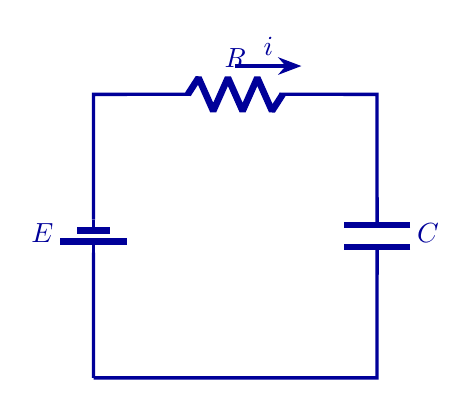
\begin{tikzpicture}[scale=1.2]
  % Symbole stylisé : circuit simple
  \draw[very thick, blue!60!black] (0,0) to[battery1, l=$E$] (0,3)
        to[R, l=$R$] (3,3)
        to[C, l=$C$] (3,0) -- (0,0);
  \draw[very thick, blue!60!black, ->, >=Stealth] (1.5,3.3) -- (2.2,3.3) node[midway, above]{$i$};
\end{tikzpicture}

\vspace{2cm}

{\large\itshape « Un bébé doit pouvoir comprendre les bases,\\
un ingénieur doit pouvoir s'y référer comme source de qualité. »}

\vspace{1.5cm}

{\large Projet Open Source — Distribution libre et gratuite}

\vfill
{\small Version 0.1 — Avril 2026}
\end{titlepage}

% === TABLE DES MATIÈRES ===
\tableofcontents
\newpage

% ============================================================================
% PARTIE I : FONDAMENTAUX
% ============================================================================
\part{Fondamentaux}

% ============================================================================
% CHAPITRE 1 : LE COURANT ÉLECTRIQUE
% ============================================================================
\chapter{Le Courant Électrique}

\begin{center}
\textit{Le courant est le mouvement ordonné de charges électriques dans un conducteur.\\
C'est la première grandeur que l'on manipule en électronique.}
\end{center}

\vspace{0.5cm}

% ----------------------------------------------------------------------------
% SECTION 1 : LES BASES
% ----------------------------------------------------------------------------
\section{Les Bases}

\begin{bases}
Cette section ne suppose aucune connaissance préalable. On part de zéro.
\end{bases}

\subsection{Qu'est-ce que le courant électrique ?}

Toute matière est composée d'\textbf{atomes}. Chaque atome possède un noyau (chargé positivement) entouré d'\textbf{électrons} (chargés négativement). Dans la plupart des matériaux solides, les électrons sont fermement liés à leur atome. Mais dans les \textbf{métaux} (cuivre, aluminium, or\ldots), certains électrons sont \textit{libres} : ils peuvent se déplacer d'atome en atome.

\begin{analogie}
\textbf{L'eau dans un tuyau.} Imaginez un tuyau rempli d'eau :
\begin{itemize}[nosep]
\item Le \textbf{tuyau} = le fil conducteur (cuivre).
\item L'\textbf{eau} = les électrons libres.
\item Le \textbf{débit d'eau} (litres par seconde) = le courant électrique.
\item La \textbf{pompe} qui met l'eau en mouvement = le générateur (pile, alimentation).
\end{itemize}
Sans pompe, l'eau ne bouge pas. Sans générateur, les électrons ne se déplacent pas de manière ordonnée.
\end{analogie}

\begin{attention}
\textbf{Limites de l'analogie hydraulique :} cette analogie est utile pour l'intuition, mais elle a des limites :
\begin{itemize}[nosep]
\item L'eau est neutre ; les électrons sont chargés et interagissent entre eux.
\item L'eau ne fait que circuler ; le courant peut aussi s'accumuler temporairement (charge d'un condensateur).
\item L'eau ne circule que dans un sens ; le courant alternatif change de sens périodiquement.
\end{itemize}
On utilisera cette analogie ponctuellement, mais en signalant toujours ses limites.
\end{attention}

Le \textbf{courant électrique}, c'est donc un \textbf{déplacement ordonné de charges} (généralement des électrons) à travers un conducteur, sous l'effet d'une force (créée par un générateur).

\subsection{Sens du courant}

Historiquement, avant la découverte de l'électron, on a \textbf{choisi par convention} que le courant circulait du pôle \textbf{+} vers le pôle \textbf{$-$} à l'extérieur du générateur.

En réalité, les électrons se déplacent dans le sens inverse : du $-$ vers le $+$.

\begin{attention}
Le \textbf{sens conventionnel} du courant (du + vers le $-$) est celui utilisé dans \textit{tous} les schémas et calculs en électronique. C'est une convention universelle. Ne la confondez jamais avec le sens réel des électrons.
\end{attention}

\begin{center}
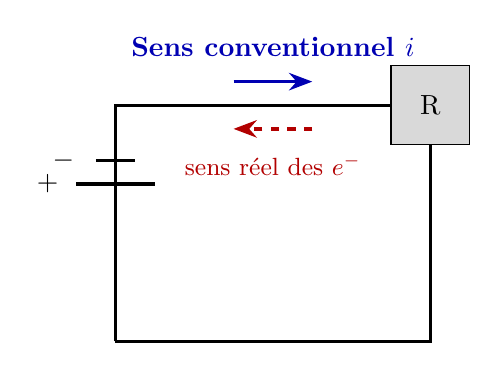
\begin{tikzpicture}[>=Stealth, scale=1.0]
  % Pile
  \draw[very thick] (0,0) -- (0,2);
  \draw[very thick] (-0.5,2) -- (0.5,2); % trait long = +
  \draw[very thick] (-0.25,2.3) -- (0.25,2.3); % trait court = -
  \node[left] at (-0.6,2) {$+$};
  \node[left] at (-0.4,2.3) {$-$};
  
  % Circuit
  \draw[very thick] (0,2) -- (0,3) -- (4,3) -- (4,0) -- (0,0);
  \draw[fill=gray!30] (3.5,2.5) rectangle (4.5,3.5);
  \node at (4,3) {R};
  
  % Sens conventionnel
  \draw[->, very thick, blue!70!black] (1.5,3.3) -- (2.5,3.3);
  \node[above, blue!70!black] at (2,3.5) {\textbf{Sens conventionnel $i$}};
  
  % Sens réel des électrons
  \draw[->, very thick, red!70!black, dashed] (2.5,2.7) -- (1.5,2.7);
  \node[below, red!70!black] at (2,2.5) {\small sens réel des $e^-$};
\end{tikzpicture}
\end{center}

\subsection{Intensité du courant}

L'\textbf{intensité} du courant mesure \textit{combien de charge} traverse une section du conducteur par unité de temps. C'est le ``débit de charges''.

\begin{formule}
\[
\boxed{I = \frac{Q}{t}}
\]
\begin{itemize}[nosep]
\item $I$ : intensité du courant, en \textbf{ampères} (A)
\item $Q$ : charge électrique qui a traversé la section, en \textbf{coulombs} (C)
\item $t$ : durée, en \textbf{secondes} (s)
\end{itemize}
\end{formule}

\textbf{Exemple :} Si $Q = \SI{10}{C}$ traversent un fil en $t = \SI{2}{s}$, alors $I = 10/2 = \SI{5}{A}$.

\begin{intuition}
Un ampère, c'est environ $6{,}24 \times 10^{18}$ électrons par seconde qui traversent la section d'un fil. C'est un nombre colossal, mais chaque électron porte si peu de charge ($\SI{1.6e-19}{C}$) que le courant résultant reste une grandeur ``humaine''.
\end{intuition}

\subsection{Ordres de grandeur}

\begin{center}
\begin{tabular}{lll}
\toprule
\textbf{Situation} & \textbf{Intensité typique} & \textbf{Ordre} \\
\midrule
Signal nerveux humain & $\sim \SI{1}{nA}$ & $10^{-9}$ A \\
LED allumée & $\sim \SI{20}{mA}$ & $10^{-2}$ A \\
Chargeur de téléphone & $\sim \SI{1}{A}$ à $\SI{3}{A}$ & $10^{0}$ A \\
Plaque de cuisson & $\sim \SI{16}{A}$ & $10^{1}$ A \\
Démarreur de voiture & $\sim \SI{200}{A}$ & $10^{2}$ A \\
Foudre & $\sim \SI{30}{kA}$ & $10^{4}$ A \\
\bottomrule
\end{tabular}
\end{center}

\subsection{Le courant continu (DC) et le courant alternatif (AC)}

\begin{itemize}
\item \textbf{Courant continu (DC)} : l'intensité est constante dans le temps. C'est le cas d'une pile, d'une batterie, d'un port USB. Le courant circule toujours dans le même sens.

\item \textbf{Courant alternatif (AC)} : l'intensité varie périodiquement (typiquement de manière sinusoïdale). C'est le cas de la prise murale (\SI{230}{V}, \SI{50}{Hz} en Europe). Le courant change de sens 100 fois par seconde.
\end{itemize}

\begin{center}
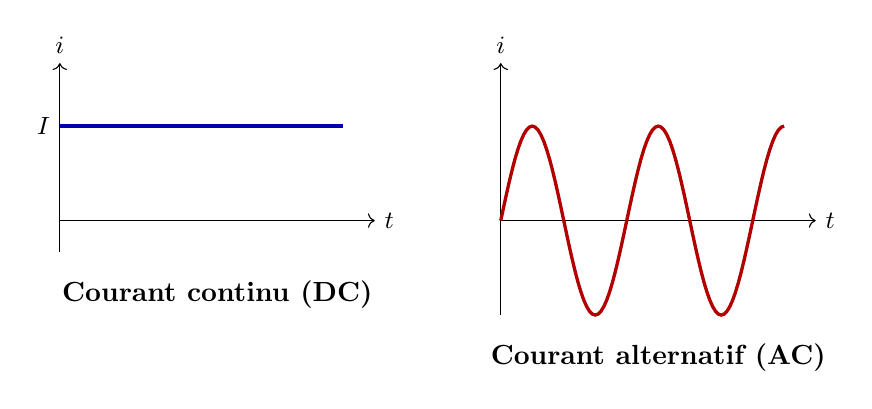
\begin{tikzpicture}[scale=0.8]
  % DC
  \begin{scope}[shift={(0,0)}]
    \draw[->] (0,0) -- (5,0) node[right]{\small $t$};
    \draw[->] (0,-0.5) -- (0,2.5) node[above]{\small $i$};
    \draw[very thick, blue!70!black] (0,1.5) -- (4.5,1.5);
    \node[below] at (2.5,-0.8) {\textbf{Courant continu (DC)}};
    \node[left] at (0,1.5) {\small $I$};
  \end{scope}
  % AC
  \begin{scope}[shift={(7,0)}]
    \draw[->] (0,0) -- (5,0) node[right]{\small $t$};
    \draw[->] (0,-1.5) -- (0,2.5) node[above]{\small $i$};
    \draw[very thick, red!70!black, domain=0:4.5, samples=100] plot(\x, {1.5*sin(180*\x)});
    \node[below] at (2.5,-1.8) {\textbf{Courant alternatif (AC)}};
  \end{scope}
\end{tikzpicture}
\end{center}

\begin{retenir}
\textbf{Ce qu'il faut retenir sur le courant :}
\begin{enumerate}[nosep]
\item Le courant est un \textbf{déplacement ordonné de charges} dans un conducteur.
\item Son intensité se mesure en \textbf{ampères} (A) : $I = Q/t$.
\item Le sens conventionnel va du $+$ au $-$ (inverse des électrons).
\item \textbf{DC} = constant, \textbf{AC} = variable (sinusoïdal en général).
\end{enumerate}
\end{retenir}

% ----------------------------------------------------------------------------
% SECTION 2 : APPROFONDISSEMENT
% ----------------------------------------------------------------------------
\section{Approfondissement}

\begin{approfondissement}
On formalise ici les notions avec les outils mathématiques adaptés. Prérequis : dérivation de base.
\end{approfondissement}

\subsection{Définition instantanée du courant}

Dans le cas général (courant variable), le courant est défini comme la dérivée de la charge par rapport au temps :

\begin{formule}
\[
\boxed{i(t) = \frac{\mathrm{d}q}{\mathrm{d}t}}
\]
C'est le débit instantané de charges à travers une section du conducteur.

Réciproquement, la charge ayant traversé entre $t_1$ et $t_2$ est :
\[
q = \int_{t_1}^{t_2} i(t)\,\mathrm{d}t
\]
\end{formule}

\textbf{Cas particulier :} si $i$ est constant (DC), alors $q = I \cdot \Delta t$ (on retrouve $I = Q/t$).

\subsection{Nature microscopique du courant}

Dans un conducteur métallique, les porteurs de charge sont les \textbf{électrons de conduction}. Chaque électron porte une charge :
\[
e = \SI{1.602e-19}{C}
\]

En l'absence de champ électrique, les électrons se déplacent de manière chaotique (agitation thermique) avec une vitesse moyenne nulle. Quand on applique un champ $\vec{E}$, il se superpose un mouvement de dérive à vitesse $\vec{v}_d$ (très lente : de l'ordre du mm/s !).

\begin{attention}
La vitesse de dérive des électrons est extrêmement faible ($\sim \SI{0.07}{mm/s}$ pour \SI{1}{A} dans du cuivre de section $\SI{1}{mm^2}$). Ce qui se propage quasi-instantanément ($\sim 2/3$ de $c$, soit $\sim \SI{2e8}{m/s}$), c'est le \textbf{champ électromagnétique} guidé par le conducteur, pas les électrons eux-mêmes. C'est comme une file de dominos : chaque domino bouge peu, mais l'information se propage vite.
\end{attention}

\subsection{Densité de courant}

On peut relier le courant macroscopique aux grandeurs microscopiques. Si un conducteur de section $S$ contient $n$ porteurs libres par unité de volume, chacun de charge $q$ et de vitesse de dérive $v_d$ :

\begin{formule}
\[
\boxed{I = n \cdot q \cdot v_d \cdot S}
\]
\begin{itemize}[nosep]
\item $n$ : densité volumique de porteurs (\si{m^{-3}})
\item $q$ : charge d'un porteur (\si{C}) — pour les électrons, $q = e$
\item $v_d$ : vitesse de dérive (\si{m/s})
\item $S$ : section du conducteur (\si{m^2})
\end{itemize}
\end{formule}

On définit le \textbf{vecteur densité de courant} :
\[
\vec{J} = n \, q \, \vec{v}_d \qquad \text{en } \si{A/m^2}
\]

Le courant total traversant une surface $S$ est alors :
\[
I = \iint_S \vec{J} \cdot \mathrm{d}\vec{S}
\]

Si $\vec{J}$ est uniforme et perpendiculaire à $S$, on retrouve $I = J \cdot S$.

\subsection{Exemple numérique : vitesse de dérive dans le cuivre}

\begin{pratique}
\textbf{Données :} fil de cuivre, section $S = \SI{1}{mm^2} = \SI{e-6}{m^2}$, courant $I = \SI{1}{A}$.

Le cuivre a une densité de porteurs $n \approx \SI{8.5e28}{m^{-3}}$.

\[
v_d = \frac{I}{n \cdot e \cdot S} = \frac{1}{8{,}5 \times 10^{28} \times 1{,}6 \times 10^{-19} \times 10^{-6}} \approx \SI{7.4e-5}{m/s} \approx \SI{0.074}{mm/s}
\]

\textbf{Conclusion :} pour \SI{1}{A}, un électron avance de $\sim \SI{0.07}{mm}$ par seconde. C'est la \textbf{propagation du champ électromagnétique} le long du conducteur ($\sim \SI{2e8}{m/s}$ dans un câble typique — cette vitesse dépend du diélectrique environnant, pas du cuivre lui-même) qui fait que la lampe s'allume quasi-instantanément quand on appuie sur l'interrupteur.
\end{pratique}

\subsection{Courant dans différents milieux}

Le courant n'existe pas que dans les métaux :

\begin{center}
\begin{tabular}{lll}
\toprule
\textbf{Milieu} & \textbf{Porteurs de charge} & \textbf{Exemple} \\
\midrule
Métaux & Électrons libres & Fil de cuivre \\
Semi-conducteurs & Électrons + trous & Silicium dopé \\
Électrolytes (liquides) & Ions ($+$ et $-$) & Batterie, électrolyse \\
Gaz ionisés (plasma) & Ions + électrons & Néon, foudre \\
Vide & Électrons & Tube cathodique \\
\bottomrule
\end{tabular}
\end{center}

% ----------------------------------------------------------------------------
% SECTION 3 : NIVEAU INGÉNIEUR
% ----------------------------------------------------------------------------
\section{Niveau Ingénieur}

\begin{ingenieur}
On fait ici le lien avec l'électromagnétisme (Maxwell), les limites des modèles, et les subtilités que l'on rencontre en conception réelle.
\end{ingenieur}

\subsection{Lien avec les équations de Maxwell : l'équation de continuité}

La conservation de la charge est un principe fondamental de la physique. Elle se traduit par l'\textbf{équation de continuité} :

\begin{formule}
\[
\boxed{\frac{\partial \rho}{\partial t} + \nabla \cdot \vec{J} = 0}
\]
\begin{itemize}[nosep]
\item $\rho$ : densité volumique de charge (\si{C/m^3})
\item $\vec{J}$ : vecteur densité de courant (\si{A/m^2})
\end{itemize}
Cette équation dit que si de la charge disparaît d'un volume, c'est qu'un courant l'a emportée. Aucune charge ne se crée ni ne disparaît.
\end{formule}

En régime stationnaire ($\partial \rho / \partial t = 0$), on obtient $\nabla \cdot \vec{J} = 0$ : la densité de courant est à \textbf{divergence nulle}, ce qui traduit que le flux de courant se conserve — c'est la justification profonde de la \textbf{loi des n\oe uds de Kirchhoff}.

\begin{attention}
Précision de vocabulaire : c'est la \textbf{charge} qui est conservée (principe fondamental). Le courant, lui, est à \textit{flux conservé} (divergence nulle) en régime stationnaire. Ne pas confondre avec un champ ``conservatif'' (dont la circulation sur un contour fermé est nulle), terme réservé au champ $\vec{E}$ en électrostatique.
\end{attention}

\subsection{Le modèle de Drude}

Le modèle de Drude (1900) est le premier modèle microscopique du courant dans les métaux. Il traite les électrons de conduction comme un gaz classique soumis à :
\begin{itemize}[nosep]
\item une force du champ électrique : $\vec{F} = -e\vec{E}$
\item des ``collisions'' avec le réseau cristallin, modélisées par un temps de relaxation $\tau$ ($\sim \SI{e-14}{s}$ dans le cuivre).
\end{itemize}

L'équation du mouvement donne en régime permanent (force de friction $-m_e\vec{v}_d/\tau$ compensant la force électrique) :
\[
\vec{0} = (-e)\vec{E} - m_e\frac{\vec{v}_d}{\tau} \quad \Longrightarrow \quad \vec{v}_d = -\frac{e\tau}{m_e}\vec{E}
\]

Le signe $-$ traduit que les électrons dérivent en sens \textit{opposé} au champ $\vec{E}$. La grandeur $\mu_e = e\tau / m_e$ est la \textbf{mobilité} des électrons.

La densité de courant s'écrit $\vec{J} = n(-e)\vec{v}_d = n(-e)\left(-\frac{e\tau}{m_e}\right)\vec{E}$, ce qui donne la \textbf{loi d'Ohm locale} :

\begin{formule}
\[
\boxed{\vec{J} = \sigma \vec{E}} \qquad \text{avec} \quad \sigma = \frac{n e^2 \tau}{m_e}
\]
$\sigma$ est la \textbf{conductivité} du matériau (\si{S/m}). Son inverse $\rho = 1/\sigma$ est la \textbf{résistivité} (\si{\ohm\cdot m}).
\end{formule}

\begin{attention}
\textbf{Limites du modèle de Drude :}
\begin{itemize}[nosep]
\item Il prédit mal la capacité thermique des métaux (corrigé par le modèle de Sommerfeld, qui traite les électrons comme des fermions).
\item Il ne rend pas compte de la structure de bandes (nécessaire pour comprendre semi-conducteurs et isolants).
\item Il ignore les effets quantiques à basse température (supraconductivité).
\end{itemize}
Malgré tout, il donne les bons ordres de grandeur pour la conductivité et justifie la loi d'Ohm.
\end{attention}

\subsection{Courant de déplacement de Maxwell}

Dans les équations de Maxwell, le théorème d'Ampère généralisé introduit un terme supplémentaire :
\[
\nabla \times \vec{B} = \mu_0 \vec{J} + \mu_0 \varepsilon_0 \frac{\partial \vec{E}}{\partial t}
\]

Le terme $\varepsilon_0 \frac{\partial \vec{E}}{\partial t}$ est le \textbf{courant de déplacement}. Ce n'est \textit{pas} un déplacement réel de charges, mais une variation temporelle du champ électrique qui produit les mêmes effets magnétiques qu'un vrai courant.

\begin{pratique}
\textbf{Application concrète :} dans un condensateur en train de se charger, aucun courant de conduction ne traverse le diélectrique. Pourtant, le champ magnétique est continu entre les armatures. C'est le courant de déplacement qui assure cette continuité. Mathématiquement, c'est le courant \textit{total} $\vec{J}_{\text{total}} = \vec{J} + \varepsilon_0 \frac{\partial \vec{E}}{\partial t}$ qui est à divergence nulle, ce qui généralise la loi des n\oe uds aux régimes variables.
\end{pratique}

\subsection{ARQS : quand peut-on utiliser Kirchhoff ?}

Les lois de Kirchhoff (loi des n\oe uds, loi des mailles) reposent sur l'\textbf{Approximation des Régimes Quasi-Stationnaires} (ARQS). Elle est valide lorsque :

\begin{formule}
\[
\boxed{d \ll \lambda = \frac{c}{f}}
\]
\begin{itemize}[nosep]
\item $d$ : dimension caractéristique du circuit
\item $\lambda$ : longueur d'onde du signal
\item $c$ : vitesse de propagation du signal dans le milieu ($\approx \SI{2e8}{m/s}$ dans un câble typique ; jusqu'à $\SI{3e8}{m/s}$ en espace libre)
\item $f$ : fréquence du signal
\end{itemize}
\end{formule}

\textbf{Règle pratique :} l'ARQS est valide tant que $d < \lambda / 10$.

\begin{center}
\begin{tabular}{lll}
\toprule
\textbf{Fréquence} & \textbf{$\lambda$ (ordre de grandeur)} & \textbf{ARQS valide si circuit $<$} \\
\midrule
\SI{50}{Hz} (secteur) & \SI{4000}{km} & \SI{400}{km} — toujours OK \\
\SI{1}{MHz} (radio AM) & \SI{200}{m} & \SI{20}{m} — OK pour un PCB \\
\SI{1}{GHz} (Wi-Fi) & \SI{20}{cm} & \SI{2}{cm} — \textbf{limite !} \\
\SI{10}{GHz} (radar) & \SI{2}{cm} & \SI{2}{mm} — ARQS rarement valide \\
\bottomrule
\end{tabular}
\end{center}

Au-delà de cette limite, il faut passer aux \textbf{lignes de transmission} et aux \textbf{équations de Maxwell complètes}.

\subsection{Effets réels à considérer en conception}

\begin{pratique}
En conception électronique réelle, le courant n'est pas aussi ``idéal'' que dans les modèles simples. Voici les phénomènes à surveiller :

\textbf{1. Effet de peau (skin effect)} — En haute fréquence, le courant ne circule plus uniformément dans la section d'un conducteur : il se concentre en surface. L'épaisseur de peau est :
\[
\delta = \sqrt{\frac{2}{\omega \mu \sigma}} = \sqrt{\frac{1}{\pi f \mu \sigma}}
\]
Pour le cuivre à \SI{1}{MHz} : $\delta \approx \SI{66}{\micro m}$. À \SI{1}{GHz} : $\delta \approx \SI{2}{\micro m}$. Cela augmente la résistance effective du conducteur et les pertes.

\textbf{2. Électromigration} — À très forte densité de courant ($> \SI{e6}{A/cm^2}$, typique des interconnexions en microélectronique), les électrons ``poussent'' physiquement les atomes du conducteur, créant des vides et éventuellement une coupure du fil. C'est un mécanisme de défaillance majeur dans les circuits intégrés.

\textbf{3. Bruit de grenaille (shot noise)} — Le courant traversant une \textit{barrière de potentiel} (jonction pn, interface métal-vide\ldots) est constitué de charges discrètes passant la barrière de manière aléatoire. Cela crée un bruit fondamental (irréductible) de densité spectrale de puissance :
\[
S_I = 2eI \qquad \text{(\si{A^2/Hz})}
\]
Ce bruit est significatif dans les circuits à très faible courant (photodiodes, amplificateurs de charges\ldots). \textit{Note :} dans un simple conducteur métallique (sans barrière), le shot noise est fortement supprimé par les corrélations entre électrons.
\end{pratique}

% === EXERCICES DU CHAPITRE 1 ===
\section*{Exercices}
\addcontentsline{toc}{section}{Exercices}

\subsection*{Niveau débutant}

\textbf{Exercice 1.1 —} Un chargeur de smartphone délivre un courant de \SI{2}{A} pendant \SI{1}{h}. Quelle charge totale a été transférée ? Combien d'électrons cela représente-t-il ?

\begin{pratique}
\textbf{Solution :} $Q = I \times t = 2 \times 3600 = \SI{7200}{C}$.
Nombre d'électrons : $N = Q/e = 7200 / 1{,}6\times10^{-19} \approx 4{,}5 \times 10^{22}$ électrons.
\end{pratique}

\textbf{Exercice 1.2 —} Une LED a besoin de \SI{20}{mA} pour fonctionner. Convertissez cette valeur en ampères. Si elle reste allumée 5 minutes, quelle charge la traverse ?

\begin{pratique}
\textbf{Solution :} $I = \SI{20}{mA} = \SI{0.020}{A}$.
Charge : $Q = I \times t = 0{,}020 \times (5 \times 60) = 0{,}020 \times 300 = \SI{6}{C}$.
\end{pratique}

\subsection*{Niveau intermédiaire}

\textbf{Exercice 1.3 —} Un courant variable est donné par $i(t) = 3\sin(100\pi t)$ (en ampères). Calculez la charge qui traverse le conducteur entre $t = 0$ et $t = \SI{10}{ms}$.

\begin{pratique}
\textbf{Solution :} $q = \int_0^{0{,}01} 3\sin(100\pi t)\,\mathrm{d}t = \left[-\frac{3}{100\pi}\cos(100\pi t)\right]_0^{0{,}01}$

$= -\frac{3}{100\pi}[\cos(\pi) - \cos(0)] = -\frac{3}{100\pi}[-1-1] = \frac{6}{100\pi} \approx \SI{19.1}{mC}$
\end{pratique}

\textbf{Exercice 1.4 —} Un fil de cuivre de section $S = \SI{1.5}{mm^2}$ transporte un courant de \SI{10}{A}. Calculez la vitesse de dérive des électrons et la densité de courant $J$. ($n_{\text{Cu}} = \SI{8.5e28}{m^{-3}}$)

\begin{pratique}
\textbf{Solution :}
Densité de courant : $J = I/S = 10 / (1{,}5 \times 10^{-6}) = \SI{6.67e6}{A/m^2} \approx \SI{6.7}{A/mm^2}$.

Vitesse de dérive : $v_d = \dfrac{I}{n \cdot e \cdot S} = \dfrac{10}{8{,}5\times10^{28} \times 1{,}6\times10^{-19} \times 1{,}5\times10^{-6}} = \dfrac{10}{2{,}04\times10^{4}} \approx \SI{4.9e-4}{m/s} \approx \SI{0.49}{mm/s}$.
\end{pratique}

\subsection*{Niveau ingénieur}

\textbf{Exercice 1.5 —} Un signal numérique à \SI{2.4}{GHz} (Wi-Fi) circule sur un PCB de \SI{10}{cm} de long. L'ARQS est-elle valide ? Justifiez quantitativement. Quel modèle faut-il utiliser à la place ?

\begin{pratique}
\textbf{Solution :} Longueur d'onde : $\lambda = c/f \approx 2\times10^8 / 2{,}4\times10^9 \approx \SI{8.3}{cm}$ (en prenant $c \approx \SI{2e8}{m/s}$ dans le FR-4).

Le PCB mesure $d = \SI{10}{cm} > \lambda/10 = \SI{0.83}{cm}$, et même $d > \lambda$ ! L'ARQS n'est \textbf{absolument pas valide}.

Il faut utiliser le modèle des \textbf{lignes de transmission} (impédance caractéristique, réflexions, adaptation).
\end{pratique}

\textbf{Exercice 1.6 —} Calculez l'épaisseur de peau dans le cuivre ($\sigma = \SI{5.8e7}{S/m}$, $\mu = \mu_0$) à \SI{50}{Hz}, \SI{1}{MHz} et \SI{1}{GHz}. Quelles conséquences pratiques pour le dimensionnement des conducteurs dans chaque cas ?

\begin{pratique}
\textbf{Solution :} $\delta = \sqrt{\dfrac{1}{\pi f \mu_0 \sigma}}$ avec $\mu_0 = 4\pi\times10^{-7}$ H/m.

\begin{itemize}[nosep]
\item $f = \SI{50}{Hz}$ : $\delta = \sqrt{\dfrac{1}{\pi \times 50 \times 4\pi\times10^{-7} \times 5{,}8\times10^7}} \approx \SI{9.3}{mm}$.

$\Rightarrow$ Le courant occupe toute la section d'un câble domestique ($\varnothing \sim$ quelques mm). Pas d'impact.

\item $f = \SI{1}{MHz}$ : $\delta \approx \SI{66}{\micro m}$.

$\Rightarrow$ Seule une couronne de $\sim\SI{66}{\micro m}$ est utilisée. Un fil plein épais est inutile : on utilise du \textbf{fil de Litz} (faisceau de brins fins isolés) pour réduire les pertes.

\item $f = \SI{1}{GHz}$ : $\delta \approx \SI{2.1}{\micro m}$.

$\Rightarrow$ Le courant circule dans une couche infime. La \textbf{rugosité de surface} du conducteur (typiquement $\sim\SI{1}{\micro m}$ sur un PCB) augmente significativement les pertes. C'est pourquoi on utilise des finitions lisses (cuivre électrodéposé, ENIG) en RF.
\end{itemize}
\end{pratique}

\subsection*{Questions de compréhension}

\begin{enumerate}[nosep]
\item Le courant conventionnel va du $+$ vers le $-$. Que se passe-t-il physiquement dans un électrolyte où les porteurs sont des ions positifs \textit{et} négatifs ?
\item Si l'on double la section d'un fil (à courant constant), que devient la densité de courant $J$ ? Et la vitesse de dérive ?
\item Pourquoi la lampe s'allume-t-elle instantanément alors que les électrons se déplacent à $\sim\SI{0.07}{mm/s}$ ?
\item Le bruit de grenaille existe-t-il dans un fil de cuivre parcouru par un courant continu ? Justifiez.
\end{enumerate}

% === RÉSUMÉ DU CHAPITRE 1 ===
\section*{Résumé du chapitre}
\addcontentsline{toc}{section}{Résumé du chapitre}

\begin{bases}[title={\color{white} Résumé --- Les Bases}]
\begin{center}
\renewcommand{\arraystretch}{1.3}
\begin{tabular}{p{4cm}p{9cm}}
\toprule
Courant & Déplacement ordonné de charges dans un conducteur \\
Intensité & $I = Q/t$ --- débit de charges --- en ampères (A) \\
Sens conventionnel & Du $+$ vers le $-$ (inverse du mouvement des $e^-$) \\
DC / AC & Continu (constant) / Alternatif (variable, souvent sinusoïdal) \\
\bottomrule
\end{tabular}
\end{center}
\end{bases}

\begin{approfondissement}[title={\color{white} Résumé --- Approfondissement}]
\begin{center}
\renewcommand{\arraystretch}{1.3}
\begin{tabular}{p{4cm}p{9cm}}
\toprule
Courant instantané & $i(t) = \mathrm{d}q/\mathrm{d}t$ \\
Densité de courant & $\vec{J} = nq\vec{v}_d$ --- $I = \iint \vec{J}\cdot\mathrm{d}\vec{S}$ \\
Vitesse de dérive & $\sim\SI{0.07}{mm/s}$ dans le cuivre pour \SI{1}{A} \\
\bottomrule
\end{tabular}
\end{center}
\end{approfondissement}

\begin{ingenieur}[title={\color{white} Résumé --- Niveau Ingénieur}]
\begin{center}
\renewcommand{\arraystretch}{1.3}
\begin{tabular}{p{4cm}p{9cm}}
\toprule
Loi d'Ohm locale & $\vec{J} = \sigma \vec{E}$ --- pont entre micro et macro \\
Conservation (charge) & $\partial\rho/\partial t + \nabla\cdot\vec{J} = 0$ --- fondement de la loi des n\oe uds \\
ARQS & Kirchhoff valide si $d \ll c/f$ \\
\bottomrule
\end{tabular}
\end{center}
\end{ingenieur}

% ============================================================================
% CHAPITRE 2 : LA TENSION ÉLECTRIQUE
% ============================================================================
\chapter{La Tension Électrique}

\begin{center}
\textit{La tension est ce qui met les charges en mouvement dans un circuit résistif.\\
C'est la ``pression'' électrique qui pousse le courant à travers les composants.}
\end{center}

\vspace{0.5cm}

% ----------------------------------------------------------------------------
% SECTION 1 : LES BASES
% ----------------------------------------------------------------------------
\section{Les Bases}

\begin{bases}
Cette section ne suppose aucune connaissance préalable. On repart de zéro.
\end{bases}

\subsection{Qu'est-ce que la tension ?}

Au chapitre précédent, on a vu que le courant est un déplacement de charges. Mais \textit{pourquoi} les charges se déplacent-elles ? Parce qu'il existe une \textbf{différence de potentiel} entre deux points du circuit. Cette différence de potentiel, c'est la \textbf{tension}.

\begin{analogie}
\textbf{La dénivellation d'eau.} Reprenons notre tuyau d'eau :
\begin{itemize}[nosep]
\item Posez un tuyau parfaitement \textbf{horizontal}, rempli d'eau : rien ne coule. L'eau est au même niveau partout.
\item \textbf{Inclinez} le tuyau : l'eau coule du point haut vers le point bas. La \textit{différence de hauteur} crée le mouvement.
\end{itemize}
En électricité, la tension joue le rôle de cette dénivellation :
\begin{itemize}[nosep]
\item La \textbf{hauteur} d'un point $\leftrightarrow$ le \textbf{potentiel électrique} de ce point.
\item La \textbf{différence de hauteur} entre deux points $\leftrightarrow$ la \textbf{tension} entre ces deux points.
\item L'eau coule du haut vers le bas $\leftrightarrow$ le courant (conventionnel) circule du potentiel haut vers le potentiel bas.
\end{itemize}
\textit{Limite :} en hydraulique, la dénivellation est absolue (liée à la gravité). En électricité, le potentiel est défini à une constante près : seule la \textit{différence} de potentiel a un sens physique.
\end{analogie}

\subsection{Définition simple}

La \textbf{tension} entre deux points A et B, notée $U_{AB}$, est la différence de potentiel électrique entre ces deux points :

\begin{formule}
\[
\boxed{U_{AB} = V_A - V_B}
\]
\begin{itemize}[nosep]
\item $U_{AB}$ : tension entre A et B, en \textbf{volts} (V)
\item $V_A$ : potentiel au point A, en volts (V)
\item $V_B$ : potentiel au point B, en volts (V)
\end{itemize}
\end{formule}

\begin{attention}
\textbf{La tension est toujours définie \textit{entre deux points}.} Dire ``la tension au point A'' n'a de sens que si l'on sous-entend un point de référence (la \textbf{masse}). C'est comme dire ``la hauteur d'une montagne'' : par rapport au niveau de la mer.
\end{attention}

\subsection{La masse (référence de potentiel)}

Dans tout circuit, on choisit un point de référence dont le potentiel est fixé à \SI{0}{V} par convention. Ce point s'appelle la \textbf{masse} (symbole : \begin{tikzpicture}[baseline=-3pt, scale=0.5]
\draw (0,0) -- (0,-0.2);
\draw (-0.3,-0.2) -- (0.3,-0.2);
\draw (-0.2,-0.35) -- (0.2,-0.35);
\draw (-0.1,-0.5) -- (0.1,-0.5);
\end{tikzpicture}).

Une fois la masse choisie, on peut parler du ``potentiel d'un point'' ou de la ``tension en un point'', ce qui signifie en réalité la tension \textit{entre ce point et la masse}.

\begin{pratique}
\textbf{En pratique :}
\begin{itemize}[nosep]
\item Sur une pile de \SI{9}{V} : la borne $-$ est à \SI{0}{V} (masse), la borne $+$ est à \SI{9}{V}.
\item Sur une alimentation symétrique $\pm\SI{15}{V}$ : la masse est au milieu, une borne est à $+\SI{15}{V}$, l'autre à $-\SI{15}{V}$.
\item Sur un PCB : le plan de masse (GND) est le conducteur commun de référence.
\end{itemize}
\end{pratique}

\subsection{Ordres de grandeur}

\begin{center}
\begin{tabular}{lll}
\toprule
\textbf{Situation} & \textbf{Tension typique} & \textbf{Ordre} \\
\midrule
Signal nerveux (potentiel d'action) & $\sim \SI{70}{mV}$ & $10^{-2}$ V \\
Pile AAA / AA & \SI{1.5}{V} & $10^{0}$ V \\
Port USB & \SI{5}{V} & $10^{0}$ V \\
Batterie de voiture & \SI{12}{V} à \SI{14}{V}& $10^{1}$ V \\
Prise secteur (Europe, efficace) & \SI{230}{V} & $10^{2}$ V \\
Ligne haute tension & \SI{400}{kV} & $10^{5}$ V \\
Foudre & $\sim \SI{100}{MV}$ & $10^{8}$ V \\
\bottomrule
\end{tabular}
\end{center}

\begin{attention}
\textbf{Danger :} une tension supérieure à environ \SI{50}{V} (en alternatif) ou \SI{120}{V} (en continu) est considérée comme \textbf{dangereuse} pour le corps humain. Le seuil de perception est d'environ \SI{1}{mA} ; la fibrillation cardiaque peut survenir dès \SI{30}{mA}. C'est le \textit{courant} qui tue, mais c'est la \textit{tension} qui le force à traverser le corps.
\end{attention}

\subsection{Tension et énergie}

La tension représente l'\textbf{énergie fournie (ou consommée) par unité de charge}. Quand une charge $q$ se déplace entre deux points A et B sous une tension $U_{AB}$, l'énergie échangée est :

\begin{formule}
\[
\boxed{W = q \cdot U}
\]
\begin{itemize}[nosep]
\item $W$ : énergie, en \textbf{joules} (J)
\item $q$ : charge, en coulombs (C)
\item $U$ : tension, en volts (V)
\end{itemize}
\vspace{0.2cm}
Autrement dit : $\SI{1}{V} = \SI{1}{J/C}$. Un volt, c'est un joule par coulomb.
\end{formule}

\subsection{Fléchage de la tension}

Sur un schéma, la tension est représentée par une \textbf{flèche} entre deux points.

\textbf{Convention :} $U_{AB} = V_A - V_B$. La flèche va \textbf{de B vers A} (du second indice vers le premier). Elle pointe vers le potentiel le plus élevé lorsque $U_{AB} > 0$.

Mnémotechnique : \textbf{la flèche de $U_{AB}$ pointe vers le ``$+$'', c'est-à-dire vers A.}

\begin{center}
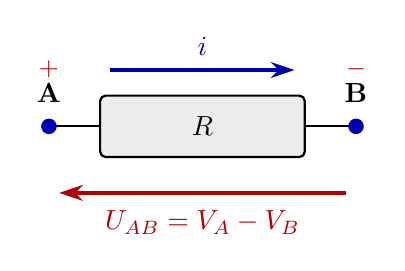
\begin{tikzpicture}[scale=1.3]
  % Dipôle (rectangle résistance)
  \draw[thick] (0,0) -- (0.5,0);
  \draw[thick, fill=gray!15, rounded corners=2pt] (0.5,-0.3) rectangle (2.5,0.3);
  \node at (1.5,0) {$R$};
  \draw[thick] (2.5,0) -- (3,0);
  
  % Points A et B
  \filldraw[blue!70!black] (0,0) circle (2pt);
  \node[above=5pt, font=\bfseries] at (0,0) {A};
  \node[above=14pt, red!70!black, font=\small] at (0,0) {$+$};
  \filldraw[blue!70!black] (3,0) circle (2pt);
  \node[above=5pt, font=\bfseries] at (3,0) {B};
  \node[above=14pt, red!70!black, font=\small] at (3,0) {$-$};
  
  % Courant i (au-dessus, de A vers B)
  \draw[line width=1.5pt, blue!70!black, -{Stealth[length=3mm, width=2mm]}] (0.6,0.55) -- (2.4,0.55);
  \node[blue!70!black, above] at (1.5,0.6) {$i$};
  
  % Flèche de tension U_AB (en dessous, DE B VERS A = de droite vers gauche)
  \draw[line width=1.5pt, red!70!black, -{Stealth[length=3mm, width=2mm]}] (2.9,-0.65) -- (0.1,-0.65);
  \node[red!70!black, below=3pt] at (1.5,-0.65) {$U_{AB} = V_A - V_B$};
\end{tikzpicture}
\end{center}

\vspace{0.3cm}
\textbf{Conventions récepteur et générateur :}

Le choix d'orientation de $i$ et $U$ sur un dipôle définit la convention utilisée :

\begin{center}
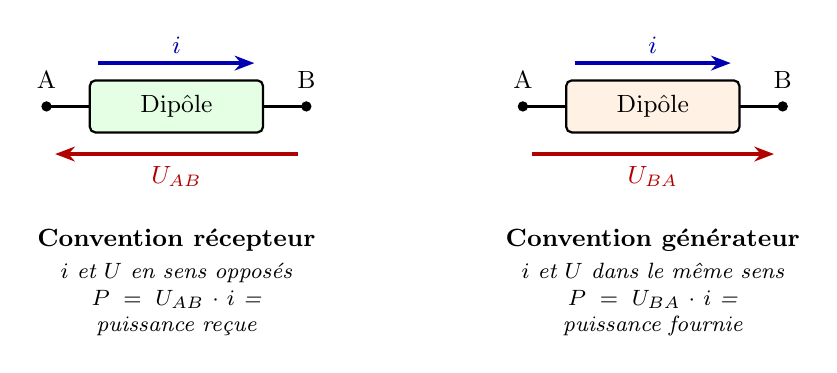
\begin{tikzpicture}[scale=1.1]
  % === Convention récepteur (gauche) ===
  \begin{scope}[shift={(0,0)}]
    \draw[thick] (0,0) -- (0.5,0);
    \draw[thick, fill=green!10, rounded corners=2pt] (0.5,-0.3) rectangle (2.5,0.3);
    \node at (1.5,0) {\small Dipôle};
    \draw[thick] (2.5,0) -- (3,0);
    
    \filldraw (0,0) circle (1.5pt) node[above=3pt]{\small A};
    \filldraw (3,0) circle (1.5pt) node[above=3pt]{\small B};
    
    % i de A vers B
    \draw[line width=1.2pt, blue!70!black, -{Stealth[length=2.5mm]}] (0.6,0.5) -- (2.4,0.5);
    \node[blue!70!black, above] at (1.5,0.5) {\small $i$};
    
    % U de B vers A (sens opposé à i)
    \draw[line width=1.2pt, red!70!black, -{Stealth[length=2.5mm]}] (2.9,-0.55) -- (0.1,-0.55);
    \node[red!70!black, below=1pt] at (1.5,-0.55) {\small $U_{AB}$};
    
    \node[below, font=\bfseries\small] at (1.5,-1.3) {Convention récepteur};
    \node[below, font=\footnotesize\itshape, text width=3.5cm, align=center] at (1.5,-1.7) {$i$ et $U$ en sens opposés\\$P = U_{AB} \cdot i$ = puissance reçue};
  \end{scope}
  
  % === Convention générateur (droite) ===
  \begin{scope}[shift={(5.5,0)}]
    \draw[thick] (0,0) -- (0.5,0);
    \draw[thick, fill=orange!10, rounded corners=2pt] (0.5,-0.3) rectangle (2.5,0.3);
    \node at (1.5,0) {\small Dipôle};
    \draw[thick] (2.5,0) -- (3,0);
    
    \filldraw (0,0) circle (1.5pt) node[above=3pt]{\small A};
    \filldraw (3,0) circle (1.5pt) node[above=3pt]{\small B};
    
    % i de A vers B
    \draw[line width=1.2pt, blue!70!black, -{Stealth[length=2.5mm]}] (0.6,0.5) -- (2.4,0.5);
    \node[blue!70!black, above] at (1.5,0.5) {\small $i$};
    
    % U de A vers B (même sens que i)
    \draw[line width=1.2pt, red!70!black, -{Stealth[length=2.5mm]}] (0.1,-0.55) -- (2.9,-0.55);
    \node[red!70!black, below=1pt] at (1.5,-0.55) {\small $U_{BA}$};
    
    \node[below, font=\bfseries\small] at (1.5,-1.3) {Convention générateur};
    \node[below, font=\footnotesize\itshape, text width=3.5cm, align=center] at (1.5,-1.7) {$i$ et $U$ dans le même sens\\$P = U_{BA} \cdot i$ = puissance fournie};
  \end{scope}
\end{tikzpicture}
\end{center}

\begin{attention}
Le fléchage est \textbf{arbitraire} : on choisit un sens, on calcule, et le \textit{signe} du résultat tranche. Si $U_{AB} < 0$, c'est que B est en réalité à un potentiel plus élevé que A. Si $i < 0$, le courant réel va en sens inverse de la flèche. Ce n'est jamais une erreur : c'est la puissance du calcul algébrique.
\end{attention}

\begin{retenir}
\textbf{Les 3 idées essentielles sur la tension :}
\begin{enumerate}[nosep]
\item La tension est toujours \textit{entre deux points} (jamais ``en un point'' sans référence).
\item C'est la tension qui met les charges en mouvement dans un circuit : pas de tension aux bornes d'une résistance $\Rightarrow$ pas de courant la traversant.
\item 1 volt = 1 joule par coulomb : la tension mesure l'énergie échangée par unité de charge.
\end{enumerate}
\end{retenir}

% ----------------------------------------------------------------------------
% SECTION 2 : APPROFONDISSEMENT
% ----------------------------------------------------------------------------
\section{Approfondissement}

\begin{approfondissement}
On formalise ici le lien entre tension, champ électrique et énergie. Prérequis : intégrale de ligne.
\end{approfondissement}

\subsection{Potentiel électrique et champ électrique}

Le \textbf{champ électrique} $\vec{E}$ est la grandeur qui décrit la force exercée sur les charges en tout point de l'espace. Pour une charge $q$ placée dans un champ $\vec{E}$ :
\[
\vec{F} = q\vec{E}
\]

Le \textbf{potentiel électrique} $V$ est relié au champ par la relation :

\begin{formule}
\[
\boxed{\vec{E} = -\vec{\nabla}V = -\operatorname{grad}(V)}
\]
En 1D (le long d'un fil) : $E = -\dfrac{\mathrm{d}V}{\mathrm{d}x}$

\vspace{0.2cm}

Le champ électrique pointe dans la direction des potentiels \textbf{décroissants}. Les charges positives suivent le champ ; les électrons vont en sens inverse.
\end{formule}

Réciproquement, la tension entre A et B est l'\textbf{intégrale de ligne} (ou circulation) du champ électrique :

\begin{formule}
\[
\boxed{U_{AB} = V_A - V_B = -\int_A^B \vec{E}\cdot\mathrm{d}\vec{\ell} = \int_B^A \vec{E}\cdot\mathrm{d}\vec{\ell}}
\]
\end{formule}

\textbf{Interprétation physique :} $U_{AB}$ représente le travail fourni par le champ électrique \textit{par unité de charge positive} lors d'un déplacement de B vers A. Si $U_{AB} > 0$, le champ favorise le mouvement des charges positives de B vers A.

\subsection{Force électromotrice (f.é.m.)}

Un générateur (pile, alternateur\ldots) \textit{fournit de l'énergie} aux charges. Il crée une \textbf{force électromotrice} (f.é.m.), notée $e$ ou $E$, qui correspond à l'énergie fournie par le générateur \textit{par unité de charge} qui le traverse :

\[
e = \frac{W_{\text{fournie}}}{q} \qquad \text{en volts (V)}
\]

\begin{attention}
Malgré son nom, la f.é.m.\ n'est \textit{pas} une force (elle s'exprime en volts, pas en newtons). C'est une tension. Le terme est historique et malheureusement trompeur.
\end{attention}

\textbf{Générateur réel vs idéal :}
\begin{itemize}[nosep]
\item \textbf{Générateur idéal} de tension : impose $U = E$ quelle que soit la charge (courant débité). N'existe pas dans la réalité.
\item \textbf{Générateur réel} : modélisé par une f.é.m.\ $E$ en série avec une résistance interne $r$. La tension aux bornes chute quand le courant augmente :
\end{itemize}

\begin{formule}
\[
\boxed{U = E - r \cdot I}
\]
\begin{itemize}[nosep]
\item $U$ : tension aux bornes du générateur (V)
\item $E$ : force électromotrice (V) — tension à vide ($I = 0$)
\item $r$ : résistance interne ($\Omega$)
\item $I$ : courant débité (A)
\end{itemize}
\end{formule}

\begin{center}
\begin{circuitikz}[scale=1.0]
  \draw (0,0) to[battery1, l=$E$, invert] (0,2)
        to[R, l=$r$] (2,2)
        -- (2,2) node[right]{A};
  \draw (0,0) -- (2,0) node[right]{B};
  \draw[<->, >=Stealth, blue!70!black] (2.5,0) -- (2.5,2) node[midway, right]{$U = E - rI$};
\end{circuitikz}
\end{center}

\subsection{Travail et puissance électrique}

Lorsqu'une charge $q$ traverse un dipôle soumis à une tension $U$ :
\begin{itemize}[nosep]
\item \textbf{Travail} (en continu) : $W = q \cdot U = U \cdot I \cdot t$
\item \textbf{Travail} (cas général) : $W = \displaystyle\int_0^t u(\tau)\cdot i(\tau)\,\mathrm{d}\tau$
\item \textbf{Puissance instantanée} (en convention récepteur) :
\end{itemize}

\begin{formule}
\[
\boxed{P = U \cdot I}
\]
$P$ en watts (W), $U$ en volts, $I$ en ampères.
\end{formule}

En convention récepteur :
\begin{itemize}[nosep]
\item $P > 0$ : le dipôle \textit{reçoit} de l'énergie (résistance, moteur\ldots).
\item $P < 0$ : le dipôle \textit{fournit} de l'énergie (il fonctionne en générateur).
\end{itemize}

\subsection{Loi d'additivité des tensions (loi des mailles — aperçu)}

Dans un circuit série, les tensions s'additionnent. Pour une maille fermée, la somme des tensions est nulle :
\[
\sum_{\text{maille}} U_k = 0
\]

C'est la \textbf{loi des mailles} (Kirchhoff), qui sera détaillée au chapitre 5. Son fondement physique : un parcours fermé ramène au même potentiel, donc la somme des ``montées'' et ``descentes'' de potentiel est nulle.

\begin{attention}
Précision : en présence de bobines (inductances), la loi des mailles reste applicable, à condition d'inclure la tension d'auto-induction $u_L = L\,\mathrm{d}i/\mathrm{d}t$ comme une tension aux bornes du composant. C'est ce que l'on fait systématiquement dans les circuits. Les limites fondamentales de la loi des mailles sont discutées dans la section Niveau Ingénieur.
\end{attention}

\begin{analogie}
Si vous faites un tour complet en montagne et revenez à votre point de départ, la somme des montées et des descentes est nulle. De même pour les potentiels le long d'une maille.
\end{analogie}

% ----------------------------------------------------------------------------
% SECTION 3 : NIVEAU INGÉNIEUR
% ----------------------------------------------------------------------------
\section{Niveau Ingénieur}

\begin{ingenieur}
Fondements électromagnétiques de la tension, limites du concept de potentiel, et pièges en haute fréquence.
\end{ingenieur}

\subsection{La tension et les équations de Maxwell}

La relation $\vec{E} = -\vec{\nabla}V$ n'est valable que si le champ électrique est \textbf{conservatif}, c'est-à-dire si sa circulation sur tout contour fermé est nulle. Or l'équation de Maxwell-Faraday dit :

\begin{formule}
\[
\boxed{\oint_{\mathcal{C}} \vec{E}\cdot\mathrm{d}\vec{\ell} = -\frac{\mathrm{d}\Phi_B}{\mathrm{d}t}}
\]
Avec $\Phi_B = \iint_S \vec{B}\cdot\mathrm{d}\vec{S}$ le flux magnétique à travers la surface délimitée par $\mathcal{C}$.
\end{formule}

\textbf{Conséquence capitale :} s'il existe un champ magnétique variable ($\mathrm{d}\Phi_B/\mathrm{d}t \neq 0$), la circulation de $\vec{E}$ sur un contour fermé n'est \textit{plus} nulle. Le champ $\vec{E}$ n'est \textit{plus} dérivable d'un potentiel scalaire.

En pratique, cela signifie que :
\begin{itemize}[nosep]
\item Le concept même de ``tension entre deux points'' devient \textbf{ambigu} : sa valeur dépend du \textit{chemin} emprunté entre les deux points.
\item La loi des mailles ($\sum U_k = 0$) n'est strictement valable qu'en ARQS.
\end{itemize}

\begin{attention}
\textbf{Le piège de la ``tension'' en présence d'induction.} Considérons une bobine dans un champ magnétique variable. Un voltmètre branché entre ses bornes mesure une certaine valeur. Mais cette valeur \textit{dépend du trajet des fils du voltmètre} ! C'est la fameuse expérience de Lewin (MIT) qui a suscité tant de débats.

En régime variable, il faut distinguer :
\begin{itemize}[nosep]
\item La \textbf{différence de potentiel} (qui n'est définie que pour la composante conservative de $\vec{E}$).
\item La \textbf{f.é.m.\ induite} (qui provient de la composante non-conservative, liée à $\partial\vec{B}/\partial t$).
\end{itemize}
La lecture d'un voltmètre donne la somme des deux le long d'un chemin particulier.
\end{attention}

\subsection{Décomposition du champ électrique en régime variable}

Pour traiter rigoureusement ce problème, on décompose le champ électrique en deux parties :
\[
\vec{E} = \underbrace{-\vec{\nabla}V}_{\text{conservative}} + \underbrace{\vec{E}_{\text{ind}}}_{\text{non-conservative}}
\]

\begin{itemize}[nosep]
\item $-\vec{\nabla}V$ : partie conservative, dérivant du potentiel $V$. C'est elle qui est liée aux charges (loi de Coulomb). Sa circulation sur un contour fermé est nulle.
\item $\vec{E}_{\text{ind}}$ : partie non-conservative (rotationnelle), liée à la variation de $\vec{B}$. C'est elle qui induit une f.é.m. Sa circulation sur un contour fermé vaut $-\mathrm{d}\Phi_B/\mathrm{d}t$.
\end{itemize}

En ARQS ($d \ll \lambda$), cette distinction est généralement inutile et la loi des mailles fonctionne tel quel. Mais dès qu'on travaille avec des bobines couplées, des transformateurs, ou en haute fréquence, cette décomposition devient essentielle.

\subsection{Bruit de tension et plancher thermique}

En conception réelle, toute résistance génère un \textbf{bruit thermique} (bruit de Johnson-Nyquist), dû à l'agitation thermique des porteurs de charge :

\begin{formule}
\[
\boxed{\overline{v_n^2} = 4 k_B T R \Delta f}
\]
\begin{itemize}[nosep]
\item $\overline{v_n^2}$ : variance de la tension de bruit (\si{V^2})
\item $k_B = \SI{1.38e-23}{J/K}$ : constante de Boltzmann
\item $T$ : température absolue (K)
\item $R$ : résistance ($\Omega$)
\item $\Delta f$ : bande passante de mesure (Hz)
\end{itemize}
\end{formule}

\begin{pratique}
\textbf{Application numérique :} une résistance de \SI{10}{k\ohm} à \SI{300}{K} (température ambiante) dans une bande passante de \SI{10}{kHz} génère un bruit de tension :
\[
v_{n,\text{eff}} = \sqrt{4 \times 1{,}38\times10^{-23} \times 300 \times 10^4 \times 10^4} = \sqrt{1{,}66\times10^{-12}} \approx \SI{1.3}{\micro V}
\]
Ce bruit est \textbf{fondamental} (irréductible) : il est fixé par les lois de la thermodynamique. Tout signal utile doit être au-dessus de ce plancher pour être détectable. C'est pourquoi les amplificateurs ultra-sensibles (radioastronomie, détection gravitationnelle) sont refroidis à quelques kelvins.
\end{pratique}

\subsection{Tension de claquage et rigidité diélectrique}

Tout isolant a une limite : au-delà d'un certain champ électrique, il devient conducteur de manière brutale. C'est le \textbf{claquage diélectrique}.

La \textbf{rigidité diélectrique} $E_{\text{max}}$ est le champ maximal que peut supporter un isolant avant claquage :

\begin{center}
\begin{tabular}{lll}
\toprule
\textbf{Matériau} & \textbf{Rigidité diélectrique} & \textbf{Épaisseur pour tenir \SI{1}{kV}} \\
\midrule
Air (sec, 1 atm) & $\sim \SI{3}{MV/m}$ & $\sim \SI{0.3}{mm}$ \\
Papier & $\sim \SI{15}{MV/m}$ & $\sim \SI{67}{\micro m}$ \\
Verre & $\sim \SI{12}{MV/m}$ & $\sim \SI{83}{\micro m}$ \\
$\text{SiO}_2$ (oxyde de grille) & $\sim \SI{500}{MV/m}$ & $\sim \SI{2}{\micro m}$ \\
\bottomrule
\end{tabular}
\end{center}

\begin{pratique}
\textbf{Implications concrètes :}
\begin{itemize}[nosep]
\item \textbf{PCB :} espacement minimal entre pistes selon la tension (normes IPC). Pour \SI{230}{V} secteur : $\geq \SI{2.5}{mm}$ entre pistes.
\item \textbf{Condensateurs :} la tension maximale d'un condensateur est limitée par le claquage de son diélectrique. Un dépassement même bref peut le détruire de manière permanente.
\item \textbf{MOSFET :} l'oxyde de grille ($\text{SiO}_2$) est extrêmement mince ($\sim$ nm). Une décharge électrostatique (ESD) de quelques volts peut le percer irréversiblement. D'où les précautions antistatiques en manipulation de composants.
\end{itemize}
\end{pratique}

% === EXERCICES DU CHAPITRE 2 ===
\section*{Exercices}
\addcontentsline{toc}{section}{Exercices}

\subsection*{Niveau débutant}

\textbf{Exercice 2.1 —} Une pile de \SI{9}{V} alimente une LED. La tension aux bornes de la LED est de \SI{2}{V} et celle aux bornes de la résistance de protection est de \SI{7}{V}. Vérifiez que la loi des mailles est respectée.

\begin{pratique}
\textbf{Solution :} Dans la maille, en parcourant dans le sens du courant : $E - U_R - U_{\text{LED}} = 0$, soit $9 - 7 - 2 = 0$ \checkmark.

La somme des tensions aux bornes des récepteurs ($\SI{7}{V} + \SI{2}{V} = \SI{9}{V}$) est bien égale à la f.é.m.\ du générateur.
\end{pratique}

\textbf{Exercice 2.2 —} Le potentiel au point A est $V_A = \SI{12}{V}$ et au point B est $V_B = \SI{5}{V}$. Calculez $U_{AB}$ et $U_{BA}$. Quel est le sens de circulation du courant conventionnel entre ces deux points ?

\begin{pratique}
\textbf{Solution :} $U_{AB} = V_A - V_B = 12 - 5 = \SI{7}{V}$. $U_{BA} = V_B - V_A = \SI{-7}{V}$.
Le courant conventionnel circule de A vers B (du potentiel haut vers le potentiel bas).
\end{pratique}

\subsection*{Niveau intermédiaire}

\textbf{Exercice 2.3 —} Une pile a une f.é.m.\ $E = \SI{4.5}{V}$ et une résistance interne $r = \SI{0.5}{\ohm}$. Elle débite un courant de \SI{1}{A}. Calculez la tension à ses bornes. Quelle puissance est dissipée dans la résistance interne ? Quel est le rendement du générateur ?

\begin{pratique}
\textbf{Solution :} $U = E - rI = 4{,}5 - 0{,}5 \times 1 = \SI{4}{V}$.
Puissance dissipée : $P_r = rI^2 = 0{,}5 \times 1^2 = \SI{0.5}{W}$.
Puissance totale : $P_E = EI = \SI{4.5}{W}$. Rendement : $\eta = U/E = 4/4{,}5 \approx 89\%$.
\end{pratique}

\textbf{Exercice 2.4 —} Un condensateur est soumis à une tension $u(t) = 10\sin(2\pi \times 50 \times t)$ V. La ``tension'' mesurée par un voltmètre est-elle cette valeur instantanée ? Quelle est la tension efficace ? (Anticipation du régime AC, à approfondir au chapitre 10.)

\begin{pratique}
\textbf{Solution :} Non, un voltmètre en mode AC mesure la \textbf{tension efficace} (RMS), pas la valeur instantanée.

Pour un signal sinusoïdal d'amplitude $\hat{U} = \SI{10}{V}$ :
\[
U_{\text{eff}} = \frac{\hat{U}}{\sqrt{2}} = \frac{10}{\sqrt{2}} \approx \SI{7.07}{V}
\]
C'est cette valeur que le voltmètre affichera. La tension crête-à-crête est $U_{\text{cc}} = 2\hat{U} = \SI{20}{V}$.
\end{pratique}

\subsection*{Niveau ingénieur}

\textbf{Exercice 2.5 —} Calculez le bruit de tension Johnson-Nyquist d'une résistance de \SI{1}{M\ohm} à \SI{27}{°C} dans une bande passante de \SI{1}{kHz}. Comparez avec le bruit d'une résistance de \SI{100}{\ohm} dans les mêmes conditions. Commentez l'impact sur le choix de la valeur de résistance dans un étage d'entrée d'amplificateur.

\begin{pratique}
\textbf{Solution :} $T = 27 + 273 = \SI{300}{K}$, $\Delta f = \SI{1}{kHz}$.

$v_{n} = \sqrt{4 k_B T R \Delta f}$

\begin{itemize}[nosep]
\item $R = \SI{1}{M\ohm}$ : $v_n = \sqrt{4 \times 1{,}38\times10^{-23} \times 300 \times 10^6 \times 10^3} = \sqrt{1{,}66\times10^{-11}} \approx \SI{4.1}{\micro V}$
\item $R = \SI{100}{\ohm}$ : $v_n = \sqrt{4 \times 1{,}38\times10^{-23} \times 300 \times 100 \times 10^3} = \sqrt{1{,}66\times10^{-15}} \approx \SI{41}{nV}$
\end{itemize}

Le bruit est 100 fois plus élevé pour la résistance 10\,000 fois plus grande (car $v_n \propto \sqrt{R}$). En entrée d'amplificateur, on préfère donc des résistances \textbf{faibles} pour minimiser le bruit thermique. C'est un compromis classique : une forte résistance donne un gain élevé mais un plancher de bruit plus haut.
\end{pratique}

\textbf{Exercice 2.6 —} Sur un PCB, deux pistes espacées de \SI{0.2}{mm} sont soumises à une différence de potentiel de \SI{100}{V}. Le diélectrique est du FR-4 (rigidité $\approx \SI{20}{MV/m}$). Y a-t-il risque de claquage ? Quel espacement minimal recommanderiez-vous avec un facteur de sécurité de 2 ?

\begin{pratique}
\textbf{Solution :} Champ appliqué : $E = U/d = 100 / (0{,}2\times10^{-3}) = \SI{500}{kV/m} = \SI{0.5}{MV/m}$.

Rigidité du FR-4 : $E_{\max} = \SI{20}{MV/m}$.

Rapport : $E/E_{\max} = 0{,}5/20 = 2{,}5\%$. Pas de risque de claquage du diélectrique.

Espacement minimal théorique : $d_{\min} = U/E_{\max} = 100/20\times10^6 = \SI{5}{\micro m}$.

Avec facteur de sécurité 2 : $d = 2 \times \SI{5}{\micro m} = \SI{10}{\micro m}$.

\textbf{Attention :} en pratique, les normes IPC imposent des distances bien plus grandes ($\sim\SI{0.6}{mm}$ pour \SI{100}{V} sur PCB) car il faut aussi considérer le claquage \textit{de surface} (creepage), la pollution, l'humidité et le vieillissement. Le calcul purement diélectrique ne suffit pas.
\end{pratique}

\subsection*{Questions de compréhension}

\begin{enumerate}[nosep]
\item Pourquoi dit-on que ``c'est le courant qui tue, pas la tension'' alors que sans tension suffisante, aucun courant dangereux ne peut traverser le corps ?
\item Un voltmètre mesure-t-il une différence de potentiel ou une f.é.m. ? Dans quels cas la distinction importe-t-elle ?
\item Une pile AA neuve a une f.é.m.\ de \SI{1.6}{V}. Quand elle vieillit, sa tension à vide reste proche de \SI{1.5}{V} mais sa tension en charge chute fortement. Quel paramètre physique a changé ?
\item Expliquez pourquoi les composants CMOS sont sensibles aux décharges électrostatiques de quelques volts seulement.
\end{enumerate}

% === RÉSUMÉ DU CHAPITRE 2 ===
\section*{Résumé du chapitre}
\addcontentsline{toc}{section}{Résumé du chapitre}

\begin{bases}[title={\color{white} Résumé --- Les Bases}]
\begin{center}
\renewcommand{\arraystretch}{1.3}
\begin{tabular}{p{4cm}p{9cm}}
\toprule
Tension & Différence de potentiel entre deux points : $U_{AB} = V_A - V_B$ (V) \\
Masse & Point de référence choisi à \SI{0}{V} \\
Énergie & $W = q \cdot U$ --- 1 volt = 1 joule par coulomb \\
Fléchage & Flèche de $U_{AB}$ pointe de B vers A (vers le $+$) \\
\bottomrule
\end{tabular}
\end{center}
\end{bases}

\begin{approfondissement}[title={\color{white} Résumé --- Approfondissement}]
\begin{center}
\renewcommand{\arraystretch}{1.3}
\begin{tabular}{p{4cm}p{9cm}}
\toprule
$\vec{E}$ et $V$ & $\vec{E} = -\vec{\nabla}V$ --- le champ dérive du potentiel \\
f.é.m. & Énergie fournie par le générateur par unité de charge (V) \\
Générateur réel & $U = E - rI$ --- la tension chute avec le courant \\
Puissance & $P = UI$ en convention récepteur \\
\bottomrule
\end{tabular}
\end{center}
\end{approfondissement}

\begin{ingenieur}[title={\color{white} Résumé --- Niveau Ingénieur}]
\begin{center}
\renewcommand{\arraystretch}{1.3}
\begin{tabular}{p{4cm}p{9cm}}
\toprule
Maxwell-Faraday & $\oint\vec{E}\cdot\mathrm{d}\vec{\ell} = -\mathrm{d}\Phi_B/\mathrm{d}t$ --- la tension perd son sens si $\vec{B}$ varie \\
Johnson-Nyquist & $\overline{v_n^2} = 4k_BTR\Delta f$ --- plancher de bruit thermique \\
Claquage & Tout isolant a une rigidité diélectrique finie \\
\bottomrule
\end{tabular}
\end{center}
\end{ingenieur}

% ============================================================================
% CHAPITRE 3 : LA RÉSISTANCE ET LA LOI D'OHM
% ============================================================================
\chapter{La Résistance et la Loi d'Ohm}

\begin{center}
\textit{La résistance est l'opposition qu'un matériau offre au passage du courant.\\
La loi d'Ohm est la relation la plus utilisée de toute l'électronique.}
\end{center}

\vspace{0.3cm}

Au chapitre 1, nous avons vu \textit{ce que} sont les charges en mouvement (le courant). Au chapitre 2, nous avons vu \textit{pourquoi} elles bougent (la tension). Ce chapitre répond à la question suivante : \textit{qu'est-ce qui freine} ce mouvement ? La réponse, c'est la résistance — et la loi qui relie les trois grandeurs, c'est la loi d'Ohm.

% ----------------------------------------------------------------------------
% SECTION 1 : LES BASES
% ----------------------------------------------------------------------------
\section{Les Bases}

\begin{bases}
Cette section ne suppose aucune connaissance préalable hormis les notions de courant et de tension (chapitres 1 et 2).
\end{bases}

\subsection{Qu'est-ce qu'une résistance ?}

Quand un courant circule dans un matériau, les porteurs de charge (électrons) sont gênés dans leur progression par les atomes du matériau. Cette opposition au passage du courant, c'est la \textbf{résistance}.

\begin{attention}
Le terme ``frottement'' est parfois utilisé pour décrire ce phénomène. C'est une image simplifiée : les électrons ne frottent pas mécaniquement contre les atomes, mais sont \textit{déviés} par eux lors de leur traversée. L'effet macroscopique est similaire : une force qui s'oppose au mouvement et dissipe de l'énergie sous forme de chaleur. Les mécanismes microscopiques exacts sont détaillés dans la section Niveau Ingénieur.
\end{attention}

\begin{analogie}
\textbf{Le tuyau étroit.} Reprenons notre analogie hydraulique :
\begin{itemize}[nosep]
\item Un tuyau \textbf{large et lisse} : l'eau coule facilement. Faible résistance.
\item Un tuyau \textbf{étroit et rugueux} : l'eau a du mal à passer. Forte résistance.
\item Plus le tuyau est \textbf{long}, plus il y a de frottements. La résistance augmente.
\item Plus le tuyau est \textbf{large} (grande section), plus le passage est facile. La résistance diminue.
\end{itemize}
\textit{Limite :} en hydraulique, le frottement dépend de la vitesse (régime laminaire vs turbulent). En électricité, pour un conducteur ohmique, la résistance est \textit{indépendante} du courant (tant que la température reste stable).
\end{analogie}

Le mot ``résistance'' désigne à la fois :
\begin{itemize}[nosep]
\item La \textbf{grandeur physique} $R$ (en ohms, $\Omega$), qui caractérise l'opposition au courant.
\item Le \textbf{composant électronique} (le ``dipôle résistif'') que l'on place dans un circuit.
\end{itemize}

\subsection{La loi d'Ohm}

La relation fondamentale entre tension, courant et résistance est la \textbf{loi d'Ohm} :

\begin{formule}
\[
\boxed{U = R \cdot I}
\]
\begin{itemize}[nosep]
\item $U$ : tension aux bornes de la résistance, en volts (V)
\item $R$ : résistance, en \textbf{ohms} ($\Omega$)
\item $I$ : courant traversant la résistance, en ampères (A)
\end{itemize}
\vspace{0.2cm}
En convention récepteur : la tension $U$ et le courant $I$ sont fléchés en sens opposé.

\vspace{0.2cm}
\textbf{Conditions de validité :} cette loi s'applique aux \textbf{conducteurs ohmiques} (ou ``linéaires''), c'est-à-dire les matériaux pour lesquels $R$ est constant quel que soit le courant. C'est le cas des résistances, des fils métalliques, des pistes de PCB\ldots{} \textit{à température constante}. Les diodes, transistors et ampoules à filament ne sont \textit{pas} ohmiques.
\end{formule}

\begin{center}
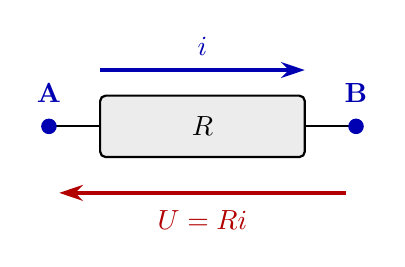
\begin{tikzpicture}[scale=1.3]
  \draw[thick] (0,0) -- (0.5,0);
  \draw[thick, fill=gray!15, rounded corners=2pt] (0.5,-0.3) rectangle (2.5,0.3);
  \node at (1.5,0) {$R$};
  \draw[thick] (2.5,0) -- (3,0);
  
  \filldraw[blue!70!black] (0,0) circle (2pt) node[above=5pt, font=\bfseries]{A};
  \filldraw[blue!70!black] (3,0) circle (2pt) node[above=5pt, font=\bfseries]{B};
  
  % Courant
  \draw[line width=1.5pt, blue!70!black, -{Stealth[length=3mm, width=2mm]}] (0.5,0.55) -- (2.5,0.55);
  \node[blue!70!black, above] at (1.5,0.6) {$i$};
  
  % Tension (convention récepteur : B vers A)
  \draw[line width=1.5pt, red!70!black, -{Stealth[length=3mm, width=2mm]}] (2.9,-0.65) -- (0.1,-0.65);
  \node[red!70!black, below=3pt] at (1.5,-0.65) {$U = Ri$};
\end{tikzpicture}
\end{center}

\begin{intuition}
La loi d'Ohm dit simplement : \textbf{plus on ``pousse'' fort (tension), plus il passe de courant}, et la résistance fixe la proportionnalité. Doubler la tension $\Rightarrow$ doubler le courant. Doubler la résistance $\Rightarrow$ diviser le courant par deux (à tension constante).
\end{intuition}

On peut reformuler la loi d'Ohm de trois façons :
\[
U = RI \qquad \Longleftrightarrow \qquad I = \frac{U}{R} \qquad \Longleftrightarrow \qquad R = \frac{U}{I}
\]

\textbf{Exemple :} une résistance de \SI{1}{k\ohm} est soumise à \SI{5}{V}. Le courant vaut $I = 5/1000 = \SI{5}{mA}$.

\subsection{Ordres de grandeur}

\begin{center}
\begin{tabular}{lll}
\toprule
\textbf{Composant / Situation} & \textbf{Résistance typique} & \textbf{Ordre} \\
\midrule
Fil de cuivre (1 m, 1.5 mm$^2$) & $\sim \SI{12}{m\ohm}$ & $10^{-2}$ $\Omega$ \\
Shunt de mesure de courant & \SI{0.1}{\ohm} à \SI{1}{\ohm} & $10^{-1}$ $\Omega$ \\
Résistance de protection LED & \SI{220}{\ohm} à \SI{1}{k\ohm} & $10^{2}$ $\Omega$ \\
Résistance de pull-up/pull-down & \SI{4.7}{k\ohm} à \SI{10}{k\ohm} & $10^{3}$ $\Omega$ \\
Corps humain (main à main, peau sèche) & $\sim \SI{1}{k\ohm}$ à \SI{100}{k\ohm} & $10^{3}$--$10^{5}$ $\Omega$ \\
Isolation d'un condensateur & $> \SI{1}{G\ohm}$ & $> 10^{9}$ $\Omega$ \\
\bottomrule
\end{tabular}
\end{center}

\subsection{Le code couleur des résistances}

Les résistances à fils (traversantes) portent des bandes de couleur qui codent leur valeur. Le code se lit de gauche à droite :

\begin{center}
\begin{tabular}{clc}
\toprule
\textbf{Couleur} & \textbf{Chiffre} & \textbf{Multiplicateur} \\
\midrule
Noir & 0 & $\times 1$ \\
Marron & 1 & $\times 10$ \\
Rouge & 2 & $\times 100$ \\
Orange & 3 & $\times 1\,000$ \\
Jaune & 4 & $\times 10\,000$ \\
Vert & 5 & $\times 100\,000$ \\
Bleu & 6 & $\times 1\,000\,000$ \\
Violet & 7 & — \\
Gris & 8 & — \\
Blanc & 9 & — \\
Or & — & $\times 0{,}1$ (tolérance $\pm 5\%$) \\
Argent & — & $\times 0{,}01$ (tolérance $\pm 10\%$) \\
\bottomrule
\end{tabular}
\end{center}

\textbf{Exemple (4 bandes) :} Marron -- Noir -- Rouge -- Or = 1 -- 0 -- $\times100$ -- $\pm5\%$ = \SI{1}{k\ohm} $\pm 5\%$.

\begin{pratique}
Mnémotechnique classique : \textit{``Ne Manger Rien Ou Jeûner, Voilà Bien Votre Grande Bêtise''} (Noir, Marron, Rouge, Orange, Jaune, Vert, Bleu, Violet, Gris, Blanc). Il en existe d'autres, à vous de choisir celle qui vous convient !
\end{pratique}

\subsection{Puissance dissipée dans une résistance}

Une résistance convertit l'énergie électrique en \textbf{chaleur} (effet Joule). La puissance dissipée est :

\begin{formule}
\[
\boxed{P = U \cdot I = R \cdot I^2 = \frac{U^2}{R}}
\]
$P$ en watts (W). Les trois formes sont équivalentes (on substitue $U = RI$).
\end{formule}

\begin{attention}
Toute résistance a une \textbf{puissance maximale admissible} (notée sur la datasheet). Si on la dépasse, elle surchauffe et peut brûler.

Valeurs typiques : \SI{0.125}{W} (1/8 W, CMS 0805), \SI{0.25}{W} (1/4 W, traversante classique), \SI{0.5}{W}, \SI{1}{W}, \SI{2}{W}\ldots

\textbf{Exemple :} une résistance de \SI{100}{\ohm} / \SI{0.25}{W}. Courant max : $I = \sqrt{P/R} = \sqrt{0{,}25/100} = \SI{50}{mA}$. Tension max : $U = \sqrt{PR} = \sqrt{0{,}25 \times 100} = \SI{5}{V}$.
\end{attention}

\subsection{Associations de résistances}

\textbf{Association série :} les résistances sont traversées par le \textbf{même courant}. Les tensions s'additionnent.

\begin{formule}
\[
\boxed{R_{\text{éq}} = R_1 + R_2 + \cdots + R_n}
\]
En série, la résistance équivalente est toujours \textbf{plus grande} que chaque résistance individuelle.
\end{formule}

\begin{center}
\begin{circuitikz}[scale=0.9]
  \draw (0,0) to[R, l=$R_1$] (2.5,0) to[R, l=$R_2$] (5,0) to[R, l=$R_3$] (7.5,0);
  \draw[line width=1.2pt, blue!70!black, -{Stealth[length=2.5mm]}] (3,0.8) -- (4.5,0.8);
  \node[blue!70!black, above] at (3.75,0.85) {\small $i$};
\end{circuitikz}
\end{center}

\textbf{Association parallèle :} les résistances sont soumises à la \textbf{même tension}. Les courants s'additionnent.

\begin{formule}
\[
\boxed{\frac{1}{R_{\text{éq}}} = \frac{1}{R_1} + \frac{1}{R_2} + \cdots + \frac{1}{R_n}}
\]
En parallèle, la résistance équivalente est toujours \textbf{plus petite} que la plus petite des résistances.

Cas particulier de 2 résistances en parallèle :
\[
R_{\text{éq}} = \frac{R_1 \cdot R_2}{R_1 + R_2} \qquad \text{(``produit sur somme'')}
\]
\end{formule}

\begin{center}
\begin{circuitikz}[scale=0.9]
  \draw (0,0) -- (1,0) -- (1,1) to[R, l=$R_1$] (4,1) -- (4,0) -- (5,0);
  \draw (1,0) -- (1,-1) to[R, l_=$R_2$] (4,-1) -- (4,0);
\end{circuitikz}
\end{center}

\begin{intuition}
\textbf{Série} = on allonge le tuyau $\Rightarrow$ plus de résistance au passage.

\textbf{Parallèle} = on ajoute un tuyau à côté $\Rightarrow$ plus de débit possible $\Rightarrow$ moins de résistance totale.
\end{intuition}

\subsection{Le diviseur de tension}

C'est le circuit le plus fondamental de l'électronique. Deux résistances en série, alimentées par une tension $E$ :

\begin{center}
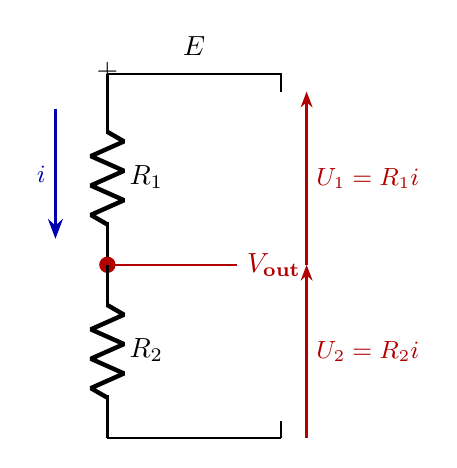
\begin{tikzpicture}[scale=1.1]
  % Source
  \draw[thick] (0,4) node[above]{$+$} -- (0,4.2);
  \draw[thick] (0,4.2) -- (2,4.2) -- (2,4);
  \node[above] at (1,4.3) {$E$};
  
  % R1
  \draw[thick] (0,4) to[R, l=$R_1$] (0,2);
  
  % Noeud Vout
  \filldraw[red!70!black] (0,2) circle (2.5pt);
  \draw[thick, red!70!black] (0,2) -- (1.5,2);
  \node[right, red!70!black, font=\bfseries] at (1.5,2) {$V_{\text{out}}$};
  
  % R2
  \draw[thick] (0,2) to[R, l=$R_2$] (0,0);
  
  % Masse
  \draw[thick] (0,0) -- (2,0);
  \draw[thick] (2,0) -- (2,0.2);
  \node[ground] at (1,0) {};
  
  % Courant
  \draw[line width=1.2pt, blue!70!black, -{Stealth[length=2.5mm]}] (-0.6,3.8) -- (-0.6,2.3);
  \node[blue!70!black, left] at (-0.6,3.05) {\small $i$};
  
  % Tensions annotées
  \draw[line width=1pt, red!70!black, -{Stealth[length=2mm]}] (2.3,2) -- (2.3,4);
  \node[red!70!black, right, font=\small] at (2.3,3) {$U_1 = R_1 i$};
  \draw[line width=1pt, red!70!black, -{Stealth[length=2mm]}] (2.3,0) -- (2.3,2);
  \node[red!70!black, right, font=\small] at (2.3,1) {$U_2 = R_2 i$};
\end{tikzpicture}
\end{center}

\begin{formule}
\[
\boxed{V_{\text{out}} = E \cdot \frac{R_2}{R_1 + R_2}}
\]
La tension de sortie est une \textbf{fraction} de la tension d'entrée, fixée par le rapport des résistances.
\end{formule}

\begin{intuition}
Pourquoi la tension se ``divise''-t-elle ? Le même courant $i = E/(R_1+R_2)$ traverse les deux résistances en série. Chacune ``consomme'' une tension proportionnelle à sa valeur ($U = Ri$). La plus grande résistance prend la plus grande part de la tension. $R_2$ récupère la fraction $R_2/(R_1+R_2)$ de $E$ : c'est un simple partage proportionnel.
\end{intuition}

\begin{attention}
Le diviseur de tension n'est valable \textbf{que si la charge en sortie ne tire pas de courant} (ou un courant négligeable devant $E/(R_1+R_2)$). Si l'on branche une charge $R_L$ en parallèle de $R_2$, la formule change : $R_2$ est remplacée par $R_2 \parallel R_L$. C'est un piège classique.
\end{attention}

\begin{retenir}
\textbf{Les 4 idées essentielles sur la résistance :}
\begin{enumerate}[nosep]
\item La résistance s'oppose au passage du courant et dissipe de l'énergie sous forme de chaleur.
\item Loi d'Ohm : $U = RI$ — relation linéaire entre tension et courant pour un conducteur ohmique.
\item Série : $R_{\text{éq}} = R_1 + R_2$. Parallèle : $R_{\text{éq}} = R_1 R_2 / (R_1 + R_2)$.
\item Diviseur de tension : $V_{\text{out}} = E \cdot R_2/(R_1+R_2)$ — valide uniquement à vide.
\end{enumerate}
\end{retenir}

% ----------------------------------------------------------------------------
% SECTION 2 : APPROFONDISSEMENT
% ----------------------------------------------------------------------------
\section{Approfondissement}

\begin{approfondissement}
On formalise les liens entre résistance, résistivité et géométrie, et on explore les dipôles non-linéaires.
\end{approfondissement}

\subsection{Résistivité et loi de Pouillet}

La résistance d'un conducteur dépend de trois facteurs : son matériau, sa longueur et sa section.

\begin{formule}
\[
\boxed{R = \rho \cdot \frac{L}{S}}
\]
\begin{itemize}[nosep]
\item $R$ : résistance ($\Omega$)
\item $\rho$ : résistivité du matériau ($\Omega\cdot$m)
\item $L$ : longueur du conducteur (m)
\item $S$ : section du conducteur (m$^2$)
\end{itemize}
\end{formule}

\begin{center}
\begin{tabular}{lll}
\toprule
\textbf{Matériau} & \textbf{Résistivité} ($\Omega\cdot$m) & \textbf{Type} \\
\midrule
Argent & $\SI{1.59e-8}{}$ & Conducteur \\
Cuivre & $\SI{1.68e-8}{}$ & Conducteur \\
Aluminium & $\SI{2.65e-8}{}$ & Conducteur \\
Fer & $\SI{9.7e-8}{}$ & Conducteur \\
Carbone & $\sim \SI{3.5e-5}{}$ & Semi-conducteur \\
Silicium (pur) & $\sim \SI{640}{}$ & Semi-conducteur \\
Verre & $\sim 10^{10}$ à $10^{14}$ & Isolant \\
\bottomrule
\end{tabular}
\end{center}

\begin{pratique}
\textbf{Application :} résistance de \SI{100}{m} de câble de cuivre de section $\SI{1.5}{mm^2}$ :
\[
R = \frac{1{,}68\times10^{-8} \times 100}{1{,}5\times10^{-6}} = \SI{1.12}{\ohm}
\]
Ce n'est pas négligeable ! Dans une installation domestique, cela représente une chute de tension de $U = RI = 1{,}12 \times 10 = \SI{11.2}{V}$ pour un appareil tirant \SI{10}{A}. C'est pourquoi la norme NF C 15-100 limite la chute de tension à $3\%$ ($\sim \SI{6.9}{V}$ sur \SI{230}{V}).
\end{pratique}

\subsection{Effet de la température}

La résistivité d'un matériau varie avec la température. Pour les \textbf{métaux}, la résistivité \textit{augmente} avec la température (les vibrations du réseau augmentent les collisions). Pour les \textbf{semi-conducteurs}, elle \textit{diminue} (la température libère des porteurs supplémentaires).

\begin{formule}
Modèle linéaire (valable sur une plage de température raisonnable) :
\[
\boxed{R(T) = R_0 \left[1 + \alpha (T - T_0)\right]}
\]
\begin{itemize}[nosep]
\item $R_0$ : résistance à la température de référence $T_0$ (souvent \SI{20}{°C} ou \SI{25}{°C})
\item $\alpha$ : coefficient de température ($\text{K}^{-1}$ ou $°C^{-1}$)
\end{itemize}
\end{formule}

\begin{center}
\begin{tabular}{ll}
\toprule
\textbf{Matériau} & $\alpha$ (\SI{}{/°C}) \\
\midrule
Cuivre & $+\SI{3.9e-3}{}$ \\
Aluminium & $+\SI{4.0e-3}{}$ \\
Platine (Pt100) & $+\SI{3.85e-3}{}$ \\
Carbone & $-\SI{5e-4}{}$ \\
\bottomrule
\end{tabular}
\end{center}

\begin{pratique}
\textbf{Sondes de température :} le fait que la résistance varie avec $T$ est exploité pour \textbf{mesurer} la température :
\begin{itemize}[nosep]
\item \textbf{Pt100 / Pt1000} : résistance en platine ($R_0 = \SI{100}{\ohm}$ ou \SI{1000}{\ohm} à \SI{0}{°C}). Très linéaire, précis, utilisé en industrie.
\item \textbf{CTN (NTC)} : thermistance à coefficient négatif. Résistance décroît fortement avec $T$. Non linéaire mais très sensible. Utilisée en électronique grand public.
\item \textbf{CTP (PTC)} : coefficient positif. Utilisée comme fusible réarmable (``polyfuse'') : si le courant est trop élevé, elle chauffe, $R$ augmente, et elle limite le courant.
\end{itemize}
\end{pratique}

\subsection{Conductance}

L'inverse de la résistance s'appelle la \textbf{conductance} :
\[
G = \frac{1}{R} \qquad \text{en siemens (S)}
\]

La loi d'Ohm s'écrit alors $I = GU$. La conductance est utile pour les calculs en parallèle :
\[
G_{\text{éq}} = G_1 + G_2 + \cdots + G_n \qquad \text{(parallèle : les conductances s'additionnent)}
\]

\subsection{Dipôles non-linéaires}

La loi d'Ohm ($U = RI$ avec $R$ constant) n'est valable que pour les \textbf{conducteurs ohmiques} (résistances, fils métalliques à température stable). Beaucoup de composants sont \textit{non-linéaires} :

\begin{center}
\begin{tabular}{ll}
\toprule
\textbf{Composant} & \textbf{Caractéristique $I(U)$} \\
\midrule
Résistance & Linéaire : $I = U/R$ (droite passant par l'origine) \\
Diode & Exponentielle : $I = I_S(e^{U/nV_T} - 1)$ \\
Ampoule à filament & Non linéaire (R augmente avec T, donc avec I) \\
Varistance (MOV) & Non linéaire, haute symétrie, seuil brutal \\
\bottomrule
\end{tabular}
\end{center}

Pour un dipôle non-linéaire, on peut définir une \textbf{résistance dynamique} (ou différentielle) au voisinage d'un point de fonctionnement :
\begin{formule}
\[
\boxed{r_d = \frac{\mathrm{d}U}{\mathrm{d}I}\bigg|_{\text{point de fonctionnement}}}
\]
C'est la pente de la caractéristique $U(I)$ au point considéré. Cette notion est fondamentale pour l'analyse des petits signaux autour du point de repos (amplificateurs, circuits à diodes\ldots).
\end{formule}

\subsection{Le pont de Wheatstone}

Le pont de Wheatstone est un circuit classique de mesure de précision. Il est constitué de quatre résistances disposées en losange, alimentées par une tension $E$ :

\begin{center}
\begin{circuitikz}[scale=1.0]
  \draw (0,2) to[R, l=$R_1$] (2,4)
        to[R, l=$R_2$] (4,2)
        to[R, l_=$R_4$] (2,0)
        to[R, l_=$R_3$] (0,2);
  \draw (2,4) -- (2,4.8) node[above]{$E$};
  \draw (2,0) -- (2,-0.5) node[below, ground]{};
  % Points A et B
  \filldraw[blue!70!black] (0,2) circle (2pt);
  \node[left=4pt, font=\bfseries] at (0,2) {A};
  \filldraw[blue!70!black] (4,2) circle (2pt);
  \node[right=4pt, font=\bfseries] at (4,2) {B};
  % Voltmètre entre A et B
  \draw[dashed, gray] (0,2) -- (1.5,2);
  \draw[dashed, gray] (2.5,2) -- (4,2);
  \node[draw, circle, inner sep=2pt, font=\small] at (2,2) {V};
\end{circuitikz}
\end{center}

Le pont est \textbf{équilibré} (le voltmètre indique $U_{AB} = 0$) lorsque :
\begin{formule}
\[
\boxed{\frac{R_1}{R_3} = \frac{R_2}{R_4}}
\]
\textbf{Remarque importante :} la condition d'équilibre ne dépend \textit{pas} de la tension d'alimentation $E$. Seuls les \textit{rapports} de résistances comptent. $E$ influence la sensibilité (amplitude de $U_{AB}$ hors équilibre) mais pas la condition d'équilibre elle-même.
\end{formule}

\begin{pratique}
\textbf{Application :} si trois résistances sont connues et l'une est inconnue, on ajuste l'une des connues jusqu'à équilibrer le pont ($U_{AB} = 0$). On en déduit la valeur inconnue avec une très grande précision. C'est le principe des jauges de contrainte (mesure de déformation mécanique), des capteurs de pression et de nombreux capteurs industriels.
\end{pratique}

% ----------------------------------------------------------------------------
% SECTION 3 : NIVEAU INGÉNIEUR
% ----------------------------------------------------------------------------
\section{Niveau Ingénieur}

\begin{ingenieur}
Loi d'Ohm locale, modèles haute fréquence, bruit, et considérations de conception réelle.
\end{ingenieur}

\subsection{Loi d'Ohm locale et résistivité tensorielle}

Au chapitre 1, on a établi la \textbf{loi d'Ohm locale} $\vec{J} = \sigma\vec{E}$. C'est l'expression microscopique dont la loi d'Ohm macroscopique $U = RI$ est une conséquence.

\textbf{Démonstration :} considérons un barreau conducteur de longueur $L$, section $S$, conductivité $\sigma$, parcouru par un courant uniforme $I$.
\begin{itemize}[nosep]
\item Le champ est uniforme : $E = U/L$ (tension aux bornes divisée par la longueur).
\item La densité de courant : $J = I/S$.
\item La loi d'Ohm locale : $J = \sigma E$, soit $I/S = \sigma \cdot U/L$.
\item On en tire : $U = \dfrac{L}{\sigma S} \cdot I = \dfrac{\rho L}{S} \cdot I = R \cdot I$. \checkmark
\end{itemize}

\begin{attention}
Dans un matériau \textbf{anisotrope} (comme certains cristaux ou composites), la conductivité n'est pas un scalaire mais un \textbf{tenseur} $\overline{\overline{\sigma}}$ : le courant ne circule pas nécessairement dans la direction du champ appliqué. On a alors $\vec{J} = \overline{\overline{\sigma}} \cdot \vec{E}$. Cela se rencontre en pratique dans les PCB multicouches (plan de cuivre vs diélectrique), les matériaux piézoélectriques, ou les semi-conducteurs sous champ magnétique (effet Hall).
\end{attention}

\subsection{Modèle haute fréquence d'une résistance}

En basse fréquence, une résistance se comporte comme une simple résistance $R$. En haute fréquence, tout composant réel possède des \textbf{éléments parasites} :

\begin{center}
\begin{circuitikz}[scale=0.9]
  \draw (0,0) to[L, l=$L_s$] (2,0) to[R, l=$R$] (4.5,0) to[short] (5.5,0);
  \draw (2.5,0) to[C, l_=$C_p$, *-*] (2.5,-1.5) -| (4,0);
  \draw (0,0) -- (-0.5,0);
  \draw (5.5,0) -- (6,0);
  \node[below] at (3,-2) {\small Modèle HF d'une résistance};
\end{circuitikz}
\end{center}

\begin{itemize}[nosep]
\item $L_s$ : \textbf{inductance série} (fils de connexion, enroulement). Typiquement quelques nH.
\item $C_p$ : \textbf{capacité parallèle} (entre les terminaux). Typiquement $< \SI{1}{pF}$.
\end{itemize}

\begin{pratique}
Conséquence : toute résistance a une \textbf{fréquence de résonance propre} $f_r = 1/(2\pi\sqrt{L_s C_p})$. Au-delà de cette fréquence, le composant ne se comporte plus du tout comme une résistance.

Ordres de grandeur de $f_r$ : CMS 0402 $\rightarrow \SI{1}{GHz}$+, traversante $\rightarrow \sim\SI{10}{MHz}$ à \SI{100}{MHz}.

Règle de conception : choisir des résistances CMS aussi petites que possible pour les circuits HF/RF.
\end{pratique}

\subsection{Bruit dans les résistances}

Une résistance génère deux types de bruit :

\textbf{1. Bruit thermique (Johnson-Nyquist)} — déjà vu au chapitre 2 :
\[
\overline{v_n^2} = 4k_B T R \Delta f
\]
Il est \textbf{indépendant} de la technologie et du matériau. Il ne dépend que de $R$, $T$ et $\Delta f$.

\textbf{2. Bruit en excès (bruit en 1/f)} — apparaît quand un courant continu traverse la résistance. Sa densité spectrale de puissance vaut approximativement :
\[
S_V(f) = \frac{K_f \cdot U_{\text{DC}}^2}{f}
\]
où $K_f$ est un coefficient qui dépend de la \textbf{technologie} de la résistance.

\textbf{Note :} cette loi en $1/f$ est \textit{empirique} — il n'existe pas de théorie unifiée expliquant le bruit en $1/f$ dans tous les systèmes. Le modèle est valide en pratique sur plusieurs décades de fréquence, mais diverge théoriquement en $f \to 0$ (ce qui n'est pas physique). En réalité, il existe toujours une fréquence basse de coupure en dessous de laquelle le spectre s'aplatit. Le coefficient $K_f$ varie d'un composant à l'autre, même au sein d'un même lot de fabrication :

\begin{center}
\begin{tabular}{ll}
\toprule
\textbf{Technologie} & \textbf{Bruit en 1/f (relatif)} \\
\midrule
Film métallique (couche mince) & Très faible \\
Film épais (thick film) & Moyen \\
Carbone (composition) & Élevé \\
Bobinée (wirewound) & Quasi nul \\
\bottomrule
\end{tabular}
\end{center}

\begin{pratique}
\textbf{Règle de conception :} pour les circuits audio ou les étages d'entrée d'instrumentation, utiliser des résistances \textbf{métal film} ou \textbf{bobinées}. Les résistances carbone sont à éviter dans les chemins de signal sensibles.
\end{pratique}

\subsection{Résistances de précision et séries normalisées (E12, E24, E96)}

Les valeurs de résistance ne sont pas arbitraires : elles suivent des \textbf{séries normalisées} (séries de Renard).

Le principe : dans chaque décade ($1 \rightarrow 10$, $10 \rightarrow 100$, etc.), on place $n$ valeurs réparties selon une progression \textbf{géométrique} de raison $r = 10^{1/n}$.

\begin{center}
\begin{tabular}{llp{7.5cm}}
\toprule
\textbf{Série} & \textbf{Tolérance} & \textbf{Valeurs dans la décade $1\rightarrow10$} \\
\midrule
E12 & $\pm 10\%$ & 1.0 -- 1.2 -- 1.5 -- 1.8 -- 2.2 -- 2.7 -- 3.3 -- 3.9 -- 4.7 -- 5.6 -- 6.8 -- 8.2 \\
E24 & $\pm 5\%$ & 24 valeurs (E12 + intermédiaires) \\
E96 & $\pm 1\%$ & 96 valeurs par décade \\
\bottomrule
\end{tabular}
\end{center}

\begin{intuition}
Pourquoi cette répartition ? Parce qu'avec une tolérance de $\pm10\%$, deux valeurs adjacentes de la série E12 se ``recouvrent'' juste : la valeur max de l'une ($\times 1{,}1$) rejoint la valeur min de la suivante ($\times 0{,}9$). Ainsi, n'importe quelle résistance réelle est couverte par l'une des valeurs de la série.
\end{intuition}

% === EXERCICES DU CHAPITRE 3 ===
\section*{Exercices}
\addcontentsline{toc}{section}{Exercices}

\subsection*{Niveau débutant}

\textbf{Exercice 3.1 —} Une résistance de \SI{470}{\ohm} est parcourue par un courant de \SI{10}{mA}. Quelle tension apparaît à ses bornes ? Quelle puissance dissipe-t-elle ?

\begin{pratique}
\textbf{Solution :} $U = RI = 470 \times 0{,}010 = \SI{4.7}{V}$.

$P = RI^2 = 470 \times (0{,}010)^2 = \SI{47}{mW}$. (Ou : $P = UI = 4{,}7 \times 0{,}010 = \SI{47}{mW}$.)

Une résistance 1/8~W (\SI{125}{mW}) suffit largement.
\end{pratique}

\textbf{Exercice 3.2 —} Quelle résistance de protection faut-il placer en série avec une LED (tension directe \SI{2}{V}, courant nominal \SI{15}{mA}) alimentée par une source de \SI{5}{V} ? Quelle puissance dissipe cette résistance ?

\begin{pratique}
\textbf{Solution :} Tension aux bornes de la résistance : $U_R = 5 - 2 = \SI{3}{V}$.

$R = U_R / I = 3 / 0{,}015 = \SI{200}{\ohm}$. Valeur normalisée la plus proche (E24) : \SI{220}{\ohm}.

Courant réel : $I = 3/220 = \SI{13.6}{mA}$ (OK pour la LED).

Puissance : $P = U_R \times I = 3 \times 0{,}0136 = \SI{41}{mW}$.
\end{pratique}

\textbf{Exercice 3.3 —} Trois résistances de \SI{100}{\ohm}, \SI{220}{\ohm} et \SI{470}{\ohm} sont placées en série. Calculez la résistance équivalente. Même question en parallèle.

\begin{pratique}
\textbf{Solution — Série :} $R_{\text{éq}} = 100 + 220 + 470 = \SI{790}{\ohm}$.

\textbf{Parallèle :} $\dfrac{1}{R_{\text{éq}}} = \dfrac{1}{100} + \dfrac{1}{220} + \dfrac{1}{470} = 0{,}01 + 0{,}00455 + 0{,}00213 = 0{,}01668$

$R_{\text{éq}} = 1/0{,}01668 \approx \SI{60}{\ohm}$.

Vérification : le résultat en parallèle ($\SI{60}{\ohm}$) est bien inférieur à la plus petite ($\SI{100}{\ohm}$). \checkmark
\end{pratique}

\subsection*{Niveau intermédiaire}

\textbf{Exercice 3.4 —} Un diviseur de tension est constitué de $R_1 = \SI{10}{k\ohm}$ et $R_2 = \SI{4.7}{k\ohm}$, alimenté par $E = \SI{12}{V}$. Calculez $V_{\text{out}}$ à vide. On branche ensuite une charge $R_L = \SI{10}{k\ohm}$ en parallèle de $R_2$. Quelle est la nouvelle tension de sortie ?

\begin{pratique}
\textbf{Solution — À vide :} $V_{\text{out}} = E \cdot \dfrac{R_2}{R_1+R_2} = 12 \times \dfrac{4700}{14700} = \SI{3.84}{V}$.

\textbf{Avec charge :} $R_2 \parallel R_L = \dfrac{4700 \times 10000}{4700 + 10000} = \dfrac{47 \times 10^6}{14700} = \SI{3197}{\ohm}$.

$V_{\text{out}} = 12 \times \dfrac{3197}{10000 + 3197} = 12 \times \dfrac{3197}{13197} = \SI{2.91}{V}$.

La tension a chuté de \SI{3.84}{V} à \SI{2.91}{V}, soit $-24\%$. Le diviseur est ``écrasé'' par la charge. \textbf{Morale :} un diviseur de tension ne fonctionne bien que si $R_L \gg R_2$.
\end{pratique}

\textbf{Exercice 3.5 —} Un câble de cuivre ($\rho = \SI{1.68e-8}{\ohm\cdot m}$) de \SI{50}{m} et de section \SI{2.5}{mm^2} alimente un appareil de \SI{3}{kW} sous \SI{230}{V}. Calculez la résistance du câble (aller + retour), la chute de tension et le pourcentage de perte.

\begin{pratique}
\textbf{Solution :} Longueur totale (aller + retour) : $L = 2 \times 50 = \SI{100}{m}$.

$R_{\text{câble}} = \rho L / S = 1{,}68\times10^{-8} \times 100 / (2{,}5\times10^{-6}) = \SI{0.672}{\ohm}$.

Courant : $I = P/U = 3000/230 = \SI{13.0}{A}$.

Chute de tension : $\Delta U = R_{\text{câble}} \times I = 0{,}672 \times 13 = \SI{8.74}{V}$, soit $8{,}74/230 = 3{,}8\%$.

C'est au-dessus de la limite normative de $3\%$ ! Il faut augmenter la section (passage en \SI{4}{mm^2}) ou raccourcir le câble.
\end{pratique}

\subsection*{Niveau ingénieur}

\textbf{Exercice 3.6 —} Une sonde Pt100 a une résistance de \SI{100}{\ohm} à \SI{0}{°C} ($\alpha = \SI{3.85e-3}{/°C}$). Elle est insérée dans un pont de Wheatstone avec trois résistances de \SI{100}{\ohm} et alimentée par \SI{5}{V}. Calculez la tension de déséquilibre $U_{AB}$ lorsque la température est de \SI{50}{°C}. Quelle sensibilité (en mV/°C) obtient-on ?

\begin{pratique}
\textbf{Solution :} Résistance de la sonde à \SI{50}{°C} :

$R_{\text{Pt}} = 100[1 + 3{,}85\times10^{-3} \times 50] = 100 \times 1{,}1925 = \SI{119.25}{\ohm}$.

Dans le pont, avec $R_1 = R_3 = R_4 = \SI{100}{\ohm}$ et $R_2 = R_{\text{Pt}} = \SI{119.25}{\ohm}$ :
\[
U_{AB} = E\left(\frac{R_2}{R_1 + R_2} - \frac{R_4}{R_3 + R_4}\right) = 5\left(\frac{119{,}25}{219{,}25} - \frac{100}{200}\right) = 5(0{,}5439 - 0{,}5) = \SI{21.9}{mV}
\]

Sensibilité : $21{,}9 / 50 \approx \SI{0.44}{mV/°C}$.

C'est un signal faible mais mesurable avec un amplificateur d'instrumentation. C'est l'architecture standard des capteurs à pont en industrie.
\end{pratique}

\textbf{Exercice 3.7 —} Une résistance CMS 0402 a une inductance parasite de \SI{0.3}{nH} et une capacité parasite de \SI{0.05}{pF}. Calculez sa fréquence de résonance. À \SI{100}{MHz}, une résistance de \SI{1}{k\ohm} se comporte-t-elle encore comme une résistance ? Justifiez.

\begin{pratique}
\textbf{Solution :} $f_r = \dfrac{1}{2\pi\sqrt{L_s C_p}} = \dfrac{1}{2\pi\sqrt{0{,}3\times10^{-9} \times 0{,}05\times10^{-12}}} = \dfrac{1}{2\pi\sqrt{1{,}5\times10^{-23}}}$

$= \dfrac{1}{2\pi \times 3{,}87\times10^{-12}} = \dfrac{1}{2{,}43\times10^{-11}} \approx \SI{41}{GHz}$.

À \SI{100}{MHz} ($\ll f_r$) : impédance de $L_s$ = $\omega L_s = 2\pi \times 10^8 \times 0{,}3\times10^{-9} = \SI{0.19}{\ohm}$ (négligeable devant \SI{1}{k\ohm}).

Impédance de $C_p$ = $1/(\omega C_p) = 1/(2\pi \times 10^8 \times 0{,}05\times10^{-12}) = \SI{31.8}{k\ohm}$ (en parallèle de $R$ : effet faible).

$\Rightarrow$ À \SI{100}{MHz}, la résistance CMS 0402 se comporte encore essentiellement comme une résistance de \SI{1}{k\ohm}. Les parasites ne deviennent gênants qu'au-delà de quelques GHz.
\end{pratique}

\subsection*{Questions de compréhension}

\begin{enumerate}[nosep]
\item Pourquoi ne peut-on pas utiliser la loi d'Ohm $U = RI$ pour une diode ?
\item Un diviseur de tension $R_1/R_2$ fournit \SI{3.3}{V} à vide. On branche un microcontrôleur qui consomme \SI{100}{mA}. Quelles sont les conséquences ? Comment dimensionner correctement ?
\item Pourquoi une résistance bobinée est-elle déconseillée en haute fréquence, malgré son faible bruit ?
\item Expliquez physiquement pourquoi la résistance d'un métal \textit{augmente} avec la température, tandis que celle d'un semi-conducteur \textit{diminue}.
\end{enumerate}

% === RÉSUMÉ DU CHAPITRE 3 ===
\section*{Résumé du chapitre}
\addcontentsline{toc}{section}{Résumé du chapitre}

\begin{bases}[title={\color{white} Résumé --- Les Bases}]
\begin{center}
\renewcommand{\arraystretch}{1.3}
\begin{tabular}{p{4cm}p{9cm}}
\toprule
Loi d'Ohm & $U = RI$ --- relation linéaire (conducteurs ohmiques) \\
Puissance (Joule) & $P = RI^2 = U^2/R$ --- dissipée en chaleur \\
Série & $R_{\text{éq}} = R_1 + R_2 + \cdots$ \\
Parallèle & $R_{\text{éq}} = R_1 R_2 / (R_1 + R_2)$ (cas 2 résistances) \\
Diviseur de tension & $V_{\text{out}} = E \cdot R_2/(R_1+R_2)$ --- valide à vide \\
\bottomrule
\end{tabular}
\end{center}
\end{bases}

\begin{approfondissement}[title={\color{white} Résumé --- Approfondissement}]
\begin{center}
\renewcommand{\arraystretch}{1.3}
\begin{tabular}{p{4cm}p{9cm}}
\toprule
Résistivité & $R = \rho L / S$ --- dépend du matériau et de la géométrie \\
Température & $R(T) = R_0[1+\alpha(T-T_0)]$ --- Pt100, CTN, CTP \\
Résistance dynamique & $r_d = \mathrm{d}U/\mathrm{d}I$ --- pour les dipôles non-linéaires \\
Pont de Wheatstone & Équilibre si $R_1/R_3 = R_2/R_4$ \\
\bottomrule
\end{tabular}
\end{center}
\end{approfondissement}

\begin{ingenieur}[title={\color{white} Résumé --- Niveau Ingénieur}]
\begin{center}
\renewcommand{\arraystretch}{1.3}
\begin{tabular}{p{4cm}p{9cm}}
\toprule
Ohm locale & $\vec{J} = \sigma\vec{E}$ --- démonstration $U = RI$ depuis le microscopique \\
Modèle HF & $R + L_s$ série $+ C_p$ parallèle --- fréquence de résonance \\
Bruit & Thermique ($4k_BTR\Delta f$) + 1/f (empirique, dépend techno) \\
Séries normalisées & E12/E24/E96 --- progression géométrique par décade \\
\bottomrule
\end{tabular}
\end{center}
\end{ingenieur}

% ============================================================================
% CHAPITRE 4 : LA PUISSANCE ET L'ÉNERGIE ÉLECTRIQUE
% ============================================================================
\chapter{La Puissance et l'Énergie Électrique}

\begin{center}
\textit{La puissance mesure le rythme auquel l'énergie est convertie.\\
C'est elle qui dimensionne les composants, les alimentations et les systèmes de refroidissement.}
\end{center}

\vspace{0.5cm}

% ----------------------------------------------------------------------------
% SECTION 1 : LES BASES
% ----------------------------------------------------------------------------
\section{Les Bases}

\begin{bases}
Cette section reprend les notions de puissance et d'énergie avec un regard global. Prérequis : chapitres 1 à 3 (courant, tension, résistance).
\end{bases}

\subsection{Puissance : définition intuitive}

La \textbf{puissance} mesure la \textit{vitesse} à laquelle l'énergie est transférée ou convertie. C'est un ``débit d'énergie''.

\begin{analogie}
\textbf{Le robinet et le seau.} On veut remplir un seau d'eau :
\begin{itemize}[nosep]
\item L'\textbf{énergie}, c'est la quantité totale d'eau dans le seau (en litres).
\item La \textbf{puissance}, c'est le débit du robinet (en litres par seconde).
\item Un robinet à fort débit (forte puissance) remplit le seau plus vite, mais la quantité d'eau finale (énergie) dépend aussi du \textit{temps} pendant lequel on laisse couler.
\end{itemize}
\end{analogie}

\subsection{Puissance électrique}

Dans un circuit électrique, la puissance échangée par un dipôle est le produit de la tension à ses bornes par le courant qui le traverse :

\begin{formule}
\[
\boxed{P = U \cdot I}
\]
\begin{itemize}[nosep]
\item $P$ : puissance, en \textbf{watts} (W)
\item $U$ : tension aux bornes du dipôle, en volts (V)
\item $I$ : courant traversant le dipôle, en ampères (A)
\end{itemize}
\vspace{0.2cm}
\textbf{Convention récepteur :} si $P > 0$, le dipôle \textit{reçoit} de l'énergie. Si $P < 0$, il en \textit{fournit}.
\end{formule}

\begin{intuition}
$P = UI$ se comprend ainsi : chaque coulomb transporte une énergie $U$ (joules par coulomb). Il passe $I$ coulombs par seconde. Donc l'énergie par seconde (= puissance) est $U \times I$.
\end{intuition}

\subsection{Puissance dissipée dans une résistance (effet Joule)}

Toute résistance convertit \textit{intégralement} l'énergie électrique en chaleur. C'est l'\textbf{effet Joule}. En combinant $P = UI$ et $U = RI$ :

\begin{formule}
\[
\boxed{P = R \cdot I^2 = \frac{U^2}{R} = U \cdot I}
\]
Ces trois formes sont équivalentes. On choisit celle qui est la plus pratique selon les données du problème.
\end{formule}

\begin{attention}
L'effet Joule est \textbf{irréversible} : on ne peut pas retransformer la chaleur en courant électrique avec une résistance. C'est une perte pure. En conception, on cherche généralement à le minimiser (sauf quand on veut chauffer : radiateur, fer à souder, fusible\ldots).
\end{attention}

\subsection{Énergie électrique}

L'énergie est la puissance intégrée sur le temps :

\begin{formule}
\[
\boxed{W = P \cdot t}
\]
\begin{itemize}[nosep]
\item $W$ : énergie, en \textbf{joules} (J)
\item $P$ : puissance, en watts (W)
\item $t$ : durée, en secondes (s)
\end{itemize}
\vspace{0.2cm}
Cette formule suppose que la puissance est constante. Si elle varie dans le temps, on utilise une intégrale (voir section Approfondissement).
\end{formule}

\begin{pratique}
\textbf{Le kilowattheure (kWh)} est l'unité d'énergie utilisée en facturation électrique :
\[
\SI{1}{kWh} = \SI{1000}{W} \times \SI{3600}{s} = \SI{3.6e6}{J} = \SI{3.6}{MJ}
\]
\textbf{Exemple :} un radiateur de \SI{2}{kW} allumé pendant 3 heures consomme $2 \times 3 = \SI{6}{kWh}$. Au tarif moyen de $\sim$0,20\,\texteuro/kWh, cela co\^ute environ 1,20\,\texteuro.
\end{pratique}

\subsection{Ordres de grandeur}

\begin{center}
\begin{tabular}{ll}
\toprule
\textbf{Appareil / Situation} & \textbf{Puissance typique} \\
\midrule
LED (indicateur) & \SI{20}{mW} à \SI{100}{mW} \\
Microcontrôleur (mode actif) & \SI{10}{mW} à \SI{500}{mW} \\
Chargeur de smartphone & \SI{5}{W} à \SI{25}{W} \\
Ordinateur portable & \SI{30}{W} à \SI{100}{W} \\
Bouilloire électrique & $\sim \SI{2}{kW}$ \\
Four électrique & $\sim \SI{3}{kW}$ \\
Voiture électrique (moteur) & \SI{50}{kW} à \SI{300}{kW} \\
TGV & $\sim \SI{9}{MW}$ \\
Centrale nucléaire (1 réacteur) & $\sim \SI{1}{GW}$ \\
\bottomrule
\end{tabular}
\end{center}

\subsection{Bilan de puissance d'un circuit}

Dans tout circuit, la puissance totale fournie par les générateurs est \textit{égale} à la puissance totale consommée par les récepteurs :

\begin{formule}
\[
\boxed{\sum P_{\text{fournie}} = \sum P_{\text{consommée}}}
\]
C'est la \textbf{conservation de l'énergie} appliquée à l'électricité. Cette relation est toujours vraie, quel que soit le circuit.
\end{formule}

\textbf{Exemple :} une pile de f.é.m.\ $E = \SI{9}{V}$, résistance interne $r = \SI{1}{\ohm}$, alimente une résistance $R = \SI{8}{\ohm}$.

Courant : $I = E/(R+r) = 9/9 = \SI{1}{A}$.

\begin{itemize}[nosep]
\item Puissance fournie par la pile : $P_E = E \cdot I = 9 \times 1 = \SI{9}{W}$.
\item Puissance dissipée dans $R$ : $P_R = RI^2 = 8 \times 1 = \SI{8}{W}$.
\item Puissance dissipée dans $r$ : $P_r = rI^2 = 1 \times 1 = \SI{1}{W}$.
\item Vérification : $P_E = P_R + P_r = 8 + 1 = \SI{9}{W}$. \checkmark
\end{itemize}

\begin{retenir}
\textbf{Les 3 idées essentielles sur la puissance :}
\begin{enumerate}[nosep]
\item $P = UI$ : la puissance est le produit tension $\times$ courant.
\item L'effet Joule ($P = RI^2$) est une perte irréversible en chaleur.
\item L'énergie, c'est la puissance accumulée dans le temps : $W = Pt$.
\end{enumerate}
\end{retenir}

% ----------------------------------------------------------------------------
% SECTION 2 : APPROFONDISSEMENT
% ----------------------------------------------------------------------------
\section{Approfondissement}

\begin{approfondissement}
Puissance en régime variable, rendement, et adaptation d'impédance. Prérequis : notions de fonctions sinusoïdales.
\end{approfondissement}

\subsection{Énergie en régime variable}

Lorsque la puissance varie dans le temps, l'énergie se calcule par intégration :
\[
W = \int_0^t p(\tau)\,\mathrm{d}\tau = \int_0^t u(\tau)\cdot i(\tau)\,\mathrm{d}\tau
\]
Si $P$ est constante, on retrouve $W = Pt$.

\subsection{Puissance instantanée et puissance moyenne}

En régime variable (AC), la tension et le courant varient dans le temps. La \textbf{puissance instantanée} est :
\[
p(t) = u(t) \cdot i(t)
\]

Elle fluctue à chaque instant. La grandeur utile en pratique est la \textbf{puissance moyenne} (ou puissance active) :

\begin{formule}
\[
\boxed{P = \langle p(t) \rangle = \frac{1}{T}\int_0^T u(t)\cdot i(t)\,\mathrm{d}t}
\]
$T$ : période du signal. $P$ est la puissance effectivement convertie en travail ou en chaleur.
\end{formule}

\subsection{Valeur efficace (RMS)}

La \textbf{valeur efficace} d'un signal périodique est la valeur continue qui dissiperait la même puissance dans une résistance :

\begin{formule}
\[
\boxed{U_{\text{eff}} = \sqrt{\frac{1}{T}\int_0^T u^2(t)\,\mathrm{d}t}} \qquad \text{(notation RMS : \textit{Root Mean Square})}
\]
\end{formule}

Pour un signal \textbf{sinusoïdal} $u(t) = \hat{U}\sin(\omega t)$ :
\[
U_{\text{eff}} = \frac{\hat{U}}{\sqrt{2}} \approx 0{,}707 \cdot \hat{U}
\]

\begin{pratique}
La prise secteur européenne délivre $\SI{230}{V}$ efficaces. Cela signifie :
\begin{itemize}[nosep]
\item Tension crête : $\hat{U} = 230 \times \sqrt{2} \approx \SI{325}{V}$.
\item Tension crête-à-crête : $U_{\text{cc}} = 2\hat{U} \approx \SI{650}{V}$.
\end{itemize}
C'est pourquoi les composants côté secteur doivent supporter \SI{400}{V} minimum (avec marge).
\end{pratique}

\begin{attention}
Un multimètre en mode AC affiche la valeur \textbf{efficace} (``True RMS'' pour les bons appareils). Les multimètres bas de gamme en mode AC ne font souvent qu'une mesure ``RMS moyenne redressée'' qui n'est correcte que pour les signaux sinusoïdaux purs. Pour les signaux déformés (PWM, carrés, triangulaires\ldots), seul un appareil ``True RMS'' donne la bonne valeur.
\end{attention}

\subsection{Rendement}

Le \textbf{rendement} $\eta$ d'un système est le rapport entre la puissance utile en sortie et la puissance totale en entrée :

\begin{formule}
\[
\boxed{\eta = \frac{P_{\text{utile}}}{P_{\text{entrée}}} = 1 - \frac{P_{\text{pertes}}}{P_{\text{entrée}}}}
\]
$\eta$ est sans dimension, compris entre 0 et 1 (souvent exprimé en \%).
\end{formule}

\begin{center}
\begin{tabular}{ll}
\toprule
\textbf{Système} & \textbf{Rendement typique} \\
\midrule
Moteur électrique (industriel) & $85\%$ à $97\%$ \\
Alimentation à découpage (SMPS)\footnote{Les régulateurs linéaires (LDO) et les convertisseurs à découpage (buck, boost, SMPS) seront détaillés dans le chapitre consacré aux alimentations.} & $80\%$ à $95\%$ \\
Régulateur linéaire (LDO)$^\text{1}$ & $\eta = V_{\text{out}}/V_{\text{in}}$ (souvent $30\%$--$70\%$) \\
Panneau solaire & $15\%$ à $25\%$ \\
Ampoule incandescente & $\sim 5\%$ (éclairage) \\
LED & $30\%$ à $50\%$ (éclairage) \\
\bottomrule
\end{tabular}
\end{center}

\begin{attention}
\textbf{Régulateur linéaire vs à découpage :} un régulateur linéaire (LDO) qui convertit \SI{12}{V} en \SI{3.3}{V} a un rendement de seulement $\eta = 3{,}3/12 = 27\%$. Les $73\%$ restants sont dissipés en chaleur. Pour un courant de \SI{1}{A}, cela fait $P_{\text{pertes}} = (12-3{,}3)\times 1 = \SI{8.7}{W}$ : il faut un radiateur ! Un convertisseur à découpage (buck) ferait le même travail avec $\eta > 90\%$, soit $< \SI{1}{W}$ de pertes.
\end{attention}

\subsection{Adaptation d'impédance et transfert maximal de puissance}

Considérons un générateur de f.é.m.\ $E$ et de résistance interne $R_s$ alimentant une charge $R_L$. La puissance délivrée à la charge est :
\[
P_L = R_L \cdot I^2 = R_L \left(\frac{E}{R_s + R_L}\right)^2
\]

En cherchant le maximum de $P_L$ par rapport à $R_L$ ($\mathrm{d}P_L/\mathrm{d}R_L = 0$), on trouve :

\begin{formule}
\[
\boxed{P_{L,\max} \text{ lorsque } R_L = R_s} \qquad \text{(adaptation d'impédance)}
\]
La puissance maximale transférée vaut alors :
\[
P_{L,\max} = \frac{E^2}{4R_s}
\]
Le rendement à adaptation est de $\eta = 50\%$ : la moitié de la puissance est dissipée dans $R_s$.
\end{formule}

\begin{intuition}
C'est un \textbf{compromis} :
\begin{itemize}[nosep]
\item $R_L \ll R_s$ : beaucoup de courant, mais presque toute la tension tombe dans $R_s$. $P_L$ est faible.
\item $R_L \gg R_s$ : presque toute la tension est aux bornes de $R_L$, mais le courant est faible. $P_L$ est aussi faible.
\item $R_L = R_s$ : le meilleur compromis entre courant et tension. $P_L$ est maximale.
\end{itemize}
\end{intuition}

\begin{pratique}
\textbf{Deux philosophies selon le domaine :}
\begin{itemize}[nosep]
\item \textbf{RF / audio / télécoms :} on adapte ($R_L = R_s = \SI{50}{\ohm}$ ou \SI{75}{\ohm}) pour maximiser le \textit{transfert de puissance} et minimiser les réflexions. Le rendement de 50\% est acceptable car les puissances sont faibles.
\item \textbf{Énergie / alimentations :} on veut $R_L \gg R_s$ pour maximiser le \textit{rendement}. On ne cherche pas le transfert maximal, mais les pertes minimales. Le rendement approche $100\%$ quand $R_L/R_s \to \infty$.
\end{itemize}
\end{pratique}

\subsection{Puissance délivrée par un générateur réel : courbe complète}

La puissance aux bornes de la charge $R_L$ en fonction de $R_L$ :

\begin{center}
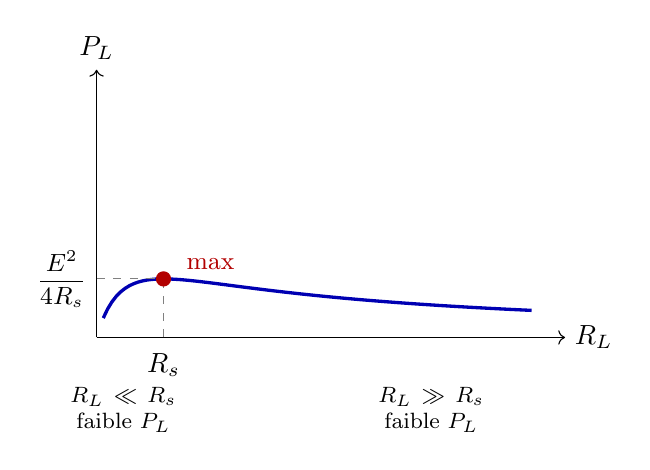
\begin{tikzpicture}[scale=0.85]
  \draw[->] (0,0) -- (7,0) node[right]{$R_L$};
  \draw[->] (0,0) -- (0,4) node[above]{$P_L$};
  
  % Courbe P_L = R_L * E^2 / (Rs + R_L)^2, normalisée
  \draw[very thick, blue!70!black, domain=0.1:6.5, samples=100] 
    plot(\x, {3.5*\x/((1+\x)*(1+\x))});
  
  % Maximum
  \draw[dashed, gray] (1,0) -- (1,3.5*1/4);
  \draw[dashed, gray] (0,3.5/4) -- (1,3.5/4);
  \filldraw[red!70!black] (1,3.5/4) circle (3pt);
  \node[below] at (1,-0.1) {$R_s$};
  \node[left, font=\small] at (0,3.5/4) {$\dfrac{E^2}{4R_s}$};
  \node[above right, red!70!black, font=\small] at (1.2,3.5/4) {max};
  
  % Annotations
  \node[below, font=\footnotesize, text width=2cm, align=center] at (0.4,-0.6) {$R_L \ll R_s$\\faible $P_L$};
  \node[below, font=\footnotesize, text width=2cm, align=center] at (5,-0.6) {$R_L \gg R_s$\\faible $P_L$};
\end{tikzpicture}
\end{center}

% ----------------------------------------------------------------------------
% SECTION 3 : NIVEAU INGÉNIEUR
% ----------------------------------------------------------------------------
\section{Niveau Ingénieur}

\begin{ingenieur}
Puissance en régime sinusoïdal complexe, facteur de puissance, et gestion thermique.
\end{ingenieur}

\subsection{Puissance en régime sinusoïdal (aperçu)}

En régime sinusoïdal permanent, si la tension et le courant sont déphasés d'un angle $\varphi$ :
\[
u(t) = \hat{U}\sin(\omega t) \qquad i(t) = \hat{I}\sin(\omega t - \varphi)
\]

La puissance instantanée contient un terme constant et un terme oscillant à $2\omega$. La puissance moyenne est :

\begin{formule}
\[
\boxed{P = U_{\text{eff}} \cdot I_{\text{eff}} \cdot \cos\varphi}
\]
\begin{itemize}[nosep]
\item $P$ : puissance active (W) — effectivement convertie en travail/chaleur
\item $\cos\varphi$ : \textbf{facteur de puissance}
\item $\varphi$ : déphasage entre tension et courant
\end{itemize}
\end{formule}

On définit également :
\begin{itemize}[nosep]
\item \textbf{Puissance apparente} : $S = U_{\text{eff}} \cdot I_{\text{eff}}$ en volt-ampères (VA).
\item \textbf{Puissance réactive} : $Q = U_{\text{eff}} \cdot I_{\text{eff}} \cdot \sin\varphi$ en volt-ampères réactifs (var).
\item Relation : $S^2 = P^2 + Q^2$.
\end{itemize}

\begin{attention}
Le facteur de puissance $\cos\varphi$ a des conséquences économiques et techniques majeures :
\begin{itemize}[nosep]
\item Un $\cos\varphi$ faible (charge inductive : moteurs, transformateurs) signifie que le réseau transporte un courant plus élevé que nécessaire pour la même puissance utile.
\item Le surdimensionnement des câbles, transformateurs et protections coûte cher.
\item Les industriels paient des \textbf{pénalités} si $\cos\varphi < 0{,}9$ (environ).
\item On corrige le $\cos\varphi$ en ajoutant des \textbf{condensateurs} (compensation réactive) ou via des correcteurs actifs (PFC).
\end{itemize}
Ce sujet sera développé en détail au chapitre sur la puissance en alternatif.
\end{attention}

\subsection{Gestion thermique : du composant au système}

Toute puissance dissipée se transforme en chaleur. La \textbf{gestion thermique} est un aspect critique de la conception électronique.

Le modèle thermique de base est analogue à la loi d'Ohm :

\begin{formule}
\[
\boxed{\Delta T = R_{\text{th}} \cdot P}
\]
\begin{itemize}[nosep]
\item $\Delta T$ : élévation de température par rapport à l'ambiante (°C ou K)
\item $R_{\text{th}}$ : résistance thermique (°C/W ou K/W)
\item $P$ : puissance dissipée (W)
\end{itemize}
\end{formule}

La résistance thermique totale entre la jonction d'un composant et l'air ambiant se décompose en série :
\[
R_{\text{th,total}} = R_{\text{th,jc}} + R_{\text{th,cs}} + R_{\text{th,sa}}
\]
\begin{itemize}[nosep]
\item $R_{\text{th,jc}}$ : jonction $\to$ boîtier (\textit{junction-to-case}), fixé par le fabricant
\item $R_{\text{th,cs}}$ : boîtier $\to$ radiateur (\textit{case-to-sink}), dépend de l'interface thermique (pâte, pad)
\item $R_{\text{th,sa}}$ : radiateur $\to$ air (\textit{sink-to-ambient}), dépend du radiateur choisi
\end{itemize}

\begin{pratique}
\textbf{Exemple de dimensionnement :} un régulateur linéaire (LDO) en boîtier TO-220 dissipe \SI{5}{W}. Sa température de jonction maximale est $T_{j,\max} = \SI{150}{°C}$. Température ambiante : $T_a = \SI{40}{°C}$. $R_{\text{th,jc}} = \SI{3}{°C/W}$, $R_{\text{th,cs}} = \SI{0.5}{°C/W}$ (avec pâte thermique).

Résistance thermique maximale du radiateur :
\[
R_{\text{th,sa}} = \frac{T_{j,\max} - T_a}{P} - R_{\text{th,jc}} - R_{\text{th,cs}} = \frac{150-40}{5} - 3 - 0{,}5 = 22 - 3{,}5 = \SI{18.5}{°C/W}
\]

Un petit radiateur à ailettes en aluminium ($\sim\SI{10}{°C/W}$) suffira largement.
\end{pratique}

\subsection{Densité spectrale de puissance et bruit (lien avec Ch.\ 2 et 3)}

En conception, le bruit est caractérisé par sa \textbf{densité spectrale de puissance} (DSP) en $\si{V^2/Hz}$ ou $\si{A^2/Hz}$. La puissance totale de bruit dans une bande $[f_1, f_2]$ est :
\[
\overline{v_n^2} = \int_{f_1}^{f_2} S_V(f)\,\mathrm{d}f
\]

Pour le bruit thermique (spectre blanc) : $S_V = 4k_BTR$, donc $\overline{v_n^2} = 4k_BTR(f_2 - f_1)$.

Pour le bruit en $1/f$ : $S_V = K/f$, donc $\overline{v_n^2} = K \ln(f_2/f_1)$.

\begin{intuition}
Le bruit blanc a la même puissance par octave en haute fréquence. Le bruit en $1/f$ a la même puissance par \textit{décade} : il domine en basse fréquence. La fréquence à laquelle les deux contributions sont égales s'appelle la \textbf{fréquence de corner} $f_c$ : c'est un paramètre clé des amplificateurs.
\end{intuition}

% === EXERCICES DU CHAPITRE 4 ===
\section*{Exercices}
\addcontentsline{toc}{section}{Exercices}

\subsection*{Niveau débutant}

\textbf{Exercice 4.1 —} Un fer à souder fonctionne sous \SI{230}{V} et consomme \SI{60}{W}. Quel courant tire-t-il ? Quelle énergie consomme-t-il en 30 minutes de fonctionnement ?

\begin{pratique}
\textbf{Solution :} $I = P/U = 60/230 = \SI{0.261}{A} \approx \SI{260}{mA}$.

Énergie : $W = P \times t = 60 \times (30 \times 60) = \SI{108000}{J} = \SI{108}{kJ}$, soit $\SI{0.030}{kWh}$.
\end{pratique}

\textbf{Exercice 4.2 —} Un chargeur USB délivre \SI{5}{V} / \SI{2}{A}. Quelle puissance fournit-il ? Combien de temps faut-il pour charger une batterie de \SI{10}{Wh} (en supposant un rendement de charge de $85\%$) ?

\begin{pratique}
\textbf{Solution :} $P = UI = 5 \times 2 = \SI{10}{W}$.

Énergie à fournir (en tenant compte du rendement) : $W_{\text{entrée}} = 10/0{,}85 = \SI{11.8}{Wh}$.

Temps : $t = W/P = 11{,}8/10 = \SI{1.18}{h} \approx \SI{1}{h}\SI{11}{min}$.
\end{pratique}

\subsection*{Niveau intermédiaire}

\textbf{Exercice 4.3 —} Un générateur ($E = \SI{24}{V}$, $r = \SI{2}{\ohm}$) alimente une charge $R_L$. Tracez qualitativement $P_L(R_L)$. Pour quelle valeur de $R_L$ la puissance est-elle maximale ? Calculez-la. Quel est le rendement à ce point ?

\begin{pratique}
\textbf{Solution :} $P_L$ maximale pour $R_L = R_s = r = \SI{2}{\ohm}$.

$P_{L,\max} = E^2/(4r) = 24^2/(4\times2) = 576/8 = \SI{72}{W}$.

Rendement : $\eta = R_L/(R_L + r) = 2/4 = 50\%$.

$I = E/(r+R_L) = 24/4 = \SI{6}{A}$. $U_L = R_L I = 2\times6 = \SI{12}{V}$ (la moitié de $E$).
\end{pratique}

\textbf{Exercice 4.4 —} La prise secteur délivre $\SI{230}{V}$ efficaces à \SI{50}{Hz}. Calculez la tension crête, la tension crête-à-crête. Un condensateur de filtrage doit-il supporter \SI{230}{V}, \SI{325}{V} ou \SI{400}{V} ? Justifiez.

\begin{pratique}
\textbf{Solution :} $\hat{U} = 230\sqrt{2} = \SI{325}{V}$. $U_{\text{cc}} = \SI{650}{V}$.

Le condensateur voit la tension \textbf{crête} (après redressement) : il doit supporter au minimum \SI{325}{V}. En pratique, on prend une marge ($+20\%$ minimum) pour les transitoires et les surtensions : on utilise un condensateur \textbf{\SI{400}{V}} (valeur normalisée).
\end{pratique}

\subsection*{Niveau ingénieur}

\textbf{Exercice 4.5 —} Un MOSFET de puissance dissipe \SI{15}{W} dans un boîtier TO-220. Ses caractéristiques : $T_{j,\max} = \SI{175}{°C}$, $R_{\text{th,jc}} = \SI{1.5}{°C/W}$. L'interface thermique a $R_{\text{th,cs}} = \SI{0.8}{°C/W}$. Température ambiante : \SI{50}{°C}. Calculez la résistance thermique maximale du radiateur et la température de jonction si l'on utilise un radiateur de \SI{4}{°C/W}.

\begin{pratique}
\textbf{Solution :} $R_{\text{th,sa,max}} = (T_{j,\max} - T_a)/P - R_{\text{th,jc}} - R_{\text{th,cs}}$

$= (175-50)/15 - 1{,}5 - 0{,}8 = 8{,}33 - 2{,}3 = \SI{6.0}{°C/W}$.

Avec un radiateur de \SI{4}{°C/W} : $R_{\text{th,total}} = 1{,}5 + 0{,}8 + 4 = \SI{6.3}{°C/W}$.

$T_j = T_a + R_{\text{th,total}} \times P = 50 + 6{,}3 \times 15 = 50 + 94{,}5 = \SI{144.5}{°C}$.

C'est sous $T_{j,\max} = \SI{175}{°C}$ : OK avec une marge de \SI{30.5}{°C}.
\end{pratique}

\textbf{Exercice 4.6 —} Un moteur industriel consomme $P_{\text{active}} = \SI{5}{kW}$ avec un $\cos\varphi = 0{,}7$ sous \SI{400}{V} (triphasé simplifié ici en monophasé). Calculez le courant absorbé, la puissance apparente et la puissance réactive. On ajoute un condensateur pour relever $\cos\varphi$ à $0{,}95$. Quelle puissance réactive doit-il compenser ?

\begin{pratique}
\textbf{Solution :} $S = P/\cos\varphi = 5000/0{,}7 = \SI{7143}{VA}$.

$I = S/U = 7143/400 = \SI{17.9}{A}$.

$Q = S\sin\varphi = 7143 \times \sin(\arccos 0{,}7) = 7143 \times 0{,}714 = \SI{5100}{var}$.

Après compensation ($\cos\varphi' = 0{,}95$) : $Q' = P\tan(\arccos 0{,}95) = 5000 \times 0{,}329 = \SI{1643}{var}$.

Le condensateur doit compenser : $Q_C = Q - Q' = 5100 - 1643 = \SI{3457}{var}$.

Le courant passe de \SI{17.9}{A} à $I' = P/(U\cos\varphi') = 5000/(400\times0{,}95) = \SI{13.2}{A}$ : réduction de $26\%$ !
\end{pratique}

\subsection*{Questions de compréhension}

\begin{enumerate}[nosep]
\item Un régulateur linéaire \SI{12}{V} $\to$ \SI{5}{V} a un rendement de $42\%$. Un convertisseur buck fait la même conversion à $92\%$. Pour un courant de \SI{2}{A}, calculez les pertes dans chaque cas. Pourquoi utilise-t-on encore des LDO malgré leur faible rendement ?
\item Pourquoi le transfert maximal de puissance ($R_L = R_s$) n'est-il \textit{pas} souhaitable pour alimenter un moteur de voiture électrique ?
\item Une résistance de \SI{10}{\ohm} / \SI{0.5}{W} est traversée par un courant de \SI{300}{mA}. Risque-t-elle de griller ? Justifiez.
\item Expliquez pourquoi un câble électrique qui chauffe de manière anormale est un signe de danger.
\end{enumerate}

% === RÉSUMÉ DU CHAPITRE 4 ===
\section*{Résumé du chapitre}
\addcontentsline{toc}{section}{Résumé du chapitre}

\begin{bases}[title={\color{white} Résumé --- Les Bases}]
\begin{center}
\renewcommand{\arraystretch}{1.3}
\begin{tabular}{p{4cm}p{9cm}}
\toprule
Puissance & $P = UI$ --- débit d'énergie (W) \\
Effet Joule & $P = RI^2$ --- perte irréversible en chaleur \\
Énergie & $W = Pt$ --- en joules (J) ou kilowattheures (kWh) \\
Bilan de puissance & $\sum P_{\text{fournie}} = \sum P_{\text{consommée}}$ \\
\bottomrule
\end{tabular}
\end{center}
\end{bases}

\begin{approfondissement}[title={\color{white} Résumé --- Approfondissement}]
\begin{center}
\renewcommand{\arraystretch}{1.3}
\begin{tabular}{p{4cm}p{9cm}}
\toprule
Valeur efficace & $U_{\text{eff}} = \hat{U}/\sqrt{2}$ (sinusoïdal) --- ``équivalent continu'' \\
Rendement & $\eta = P_{\text{utile}}/P_{\text{entrée}}$ \\
Adaptation & $P_{L,\max}$ quand $R_L = R_s$ --- rendement 50\% \\
\bottomrule
\end{tabular}
\end{center}
\end{approfondissement}

\begin{ingenieur}[title={\color{white} Résumé --- Niveau Ingénieur}]
\begin{center}
\renewcommand{\arraystretch}{1.3}
\begin{tabular}{p{4cm}p{9cm}}
\toprule
Facteur de puissance & $P = UI\cos\varphi$ --- $\cos\varphi < 1$ = courant gaspillé \\
Thermique & $\Delta T = R_{\text{th}} \cdot P$ --- analogie Ohm pour la chaleur \\
DSP de bruit & Blanc $4k_BTR$ + 1/f --- fréquence de corner $f_c$ \\
\bottomrule
\end{tabular}
\end{center}
\end{ingenieur}

% ============================================================================
% CHAPITRE 5 : LES LOIS DE KIRCHHOFF
% ============================================================================
\chapter{Les Lois de Kirchhoff}

\begin{center}
\textit{Deux lois, deux principes physiques fondamentaux :\\
la conservation de la charge et la conservation de l'énergie.\\
Combinées à la loi d'Ohm, elles permettent de résoudre tout circuit.}
\end{center}

\vspace{0.5cm}

% ----------------------------------------------------------------------------
% SECTION 1 : LES BASES
% ----------------------------------------------------------------------------
\section{Les Bases}

\begin{bases}
Cette section introduit les deux lois de Kirchhoff de manière intuitive, sans formalisme avancé. Prérequis : courant, tension, résistance (chapitres 1 à 3).
\end{bases}

\subsection{Vocabulaire des circuits}

Avant d'énoncer les lois, il faut maîtriser le vocabulaire :

\begin{itemize}
\item \textbf{Branche :} portion de circuit entre deux n\oe uds, parcourue par un \textit{seul} courant. Une branche contient un ou plusieurs composants en série.
\item \textbf{N\oe ud :} point de connexion où \textit{au moins trois} branches se rejoignent. C'est un carrefour de courants.
\item \textbf{Maille :} tout parcours fermé dans le circuit, en suivant des branches bout à bout, qui revient au point de départ sans passer deux fois par la même branche.
\end{itemize}

\begin{center}
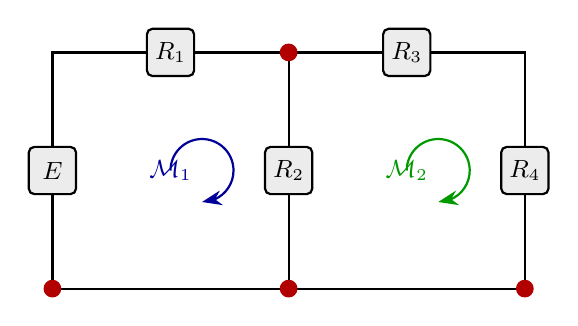
\begin{tikzpicture}[scale=1.0]
  % Circuit exemple
  \draw[thick] (0,0) -- (0,3) -- (3,3) -- (3,0) -- (0,0);
  \draw[thick] (3,3) -- (6,3) -- (6,0) -- (3,0);
  
  % Composants
  \draw[thick, fill=gray!15, rounded corners=2pt] (-0.3,1.2) rectangle (0.3,1.8);
  \node[font=\small] at (0,1.5) {$E$};
  \draw[thick, fill=gray!15, rounded corners=2pt] (1.2,2.7) rectangle (1.8,3.3);
  \node[font=\small] at (1.5,3) {$R_1$};
  \draw[thick, fill=gray!15, rounded corners=2pt] (2.7,1.2) rectangle (3.3,1.8);
  \node[font=\small] at (3,1.5) {$R_2$};
  \draw[thick, fill=gray!15, rounded corners=2pt] (4.2,2.7) rectangle (4.8,3.3);
  \node[font=\small] at (4.5,3) {$R_3$};
  \draw[thick, fill=gray!15, rounded corners=2pt] (5.7,1.2) rectangle (6.3,1.8);
  \node[font=\small] at (6,1.5) {$R_4$};
  
  % Noeuds
  \filldraw[red!70!black] (0,0) circle (3pt);
  \filldraw[red!70!black] (3,0) circle (3pt);
  \filldraw[red!70!black] (3,3) circle (3pt);
  \filldraw[red!70!black] (6,0) circle (3pt);
  
  % Mailles
  \draw[-{Stealth[length=2.5mm]}, blue!60!black, thick] (1.5,1.5) arc[start angle=180, end angle=-90, radius=0.4];
  \node[blue!60!black, font=\small] at (1.5,1.5) {$\mathcal{M}_1$};
  \draw[-{Stealth[length=2.5mm]}, green!60!black, thick] (4.5,1.5) arc[start angle=180, end angle=-90, radius=0.4];
  \node[green!60!black, font=\small] at (4.5,1.5) {$\mathcal{M}_2$};
\end{tikzpicture}
\end{center}

\subsection{Loi des n\oe uds (KCL)}

\begin{formule}
\textbf{Loi des n\oe uds :} en tout n\oe ud d'un circuit, la somme des courants entrants est égale à la somme des courants sortants :
\[
\boxed{\sum i_{\text{entrants}} = \sum i_{\text{sortants}}}
\]
Forme algébrique (entrants $+$, sortants $-$) : $\displaystyle\sum_{k} i_k = 0$.
\end{formule}

\begin{center}
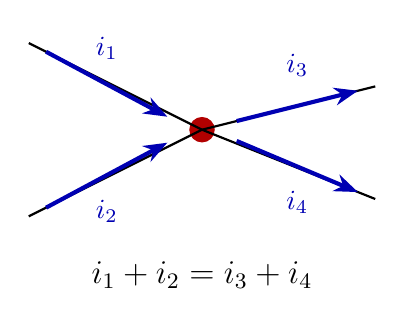
\begin{tikzpicture}[scale=1.1]
  \filldraw[red!70!black] (0,0) circle (4pt);
  \draw[thick] (-2,1) -- (0,0);
  \draw[thick] (-2,-1) -- (0,0);
  \draw[thick] (2,0.5) -- (0,0);
  \draw[thick] (2,-0.8) -- (0,0);
  
  \draw[line width=1.5pt, blue!70!black, -{Stealth[length=3mm]}] (-1.8,0.9) -- (-0.4,0.15);
  \node[blue!70!black, above] at (-1.1,0.7) {$i_1$};
  \draw[line width=1.5pt, blue!70!black, -{Stealth[length=3mm]}] (-1.8,-0.9) -- (-0.4,-0.15);
  \node[blue!70!black, below] at (-1.1,-0.7) {$i_2$};
  \draw[line width=1.5pt, blue!70!black, -{Stealth[length=3mm]}] (0.4,0.1) -- (1.8,0.45);
  \node[blue!70!black, above] at (1.1,0.5) {$i_3$};
  \draw[line width=1.5pt, blue!70!black, -{Stealth[length=3mm]}] (0.4,-0.13) -- (1.8,-0.72);
  \node[blue!70!black, below] at (1.1,-0.6) {$i_4$};
  
  \node[below=1cm, font=\large] at (0,-0.5) {$i_1 + i_2 = i_3 + i_4$};
\end{tikzpicture}
\end{center}

\begin{analogie}
\textbf{Le carrefour hydraulique.} À un embranchement de tuyaux, l'eau qui arrive doit repartir intégralement : il n'y a pas d'accumulation au carrefour. De même, en régime permanent, la charge électrique ne s'accumule pas aux n\oe uds.
\end{analogie}

\begin{intuition}
\textbf{Pourquoi ça marche :} la loi des n\oe uds traduit un principe fondamental de la physique, la \textbf{conservation de la charge}. En régime permanent, chaque coulomb qui arrive à un n\oe ud en repart. Pas un de plus, pas un de moins.
\end{intuition}

\subsection{Loi des mailles (KVL)}

\begin{formule}
\textbf{Loi des mailles :} le long de toute maille fermée, la somme algébrique des tensions est nulle :
\[
\boxed{\sum_{\text{maille}} U_k = 0}
\]
On choisit un sens de parcours. Une tension est comptée $+$ si sa flèche est dans le sens du parcours, $-$ sinon.
\end{formule}

\begin{analogie}
\textbf{La randonnée en boucle.} Si vous partez d'un refuge, faites une boucle en montagne et revenez au refuge, votre altitude finale est la même que votre altitude de départ. La somme des montées et des descentes est nécessairement nulle. De même, chaque résistance est une ``descente'' de potentiel, chaque générateur une ``montée''.
\end{analogie}

\begin{intuition}
\textbf{Pourquoi ça marche :} quand on parcourt une maille fermée, on revient au même point, donc au même potentiel. La somme des variations de potentiel le long du parcours est forcément nulle. C'est une conséquence directe du fait que la tension est une \textit{différence de potentiel}.
\end{intuition}

\begin{attention}
\textbf{Piège classique --- les signes.} Lors du parcours d'une maille :
\begin{itemize}[nosep]
\item Si l'on traverse une résistance \textit{dans le sens du courant} : la tension est une \textbf{chute} $-RI$.
\item Si l'on traverse un générateur du $-$ vers le $+$ : c'est une \textbf{montée} $+E$.
\end{itemize}
Le signe dépend du \textit{sens de parcours choisi}, pas du sens réel du courant (qu'on ne connaît pas encore). Si le calcul donne un courant négatif, c'est que le sens réel est l'inverse de celui supposé.
\end{attention}

\subsection{Méthode de résolution}

\begin{enumerate}
\item \textbf{Repérer} les n\oe uds, branches et mailles.
\item \textbf{Choisir} un sens de courant (arbitraire) dans chaque branche.
\item \textbf{Flécher} les tensions (convention récepteur pour les résistances).
\item \textbf{Écrire} les équations : $n-1$ lois des n\oe uds + $b - n + 1$ lois des mailles ($b$ branches, $n$ n\oe uds).
\item \textbf{Résoudre} le système.
\item \textbf{Vérifier} : bilan de puissance, signes, ordres de grandeur.
\end{enumerate}

\subsection{Exemple complet résolu}

\textbf{Énoncé :} $E = \SI{12}{V}$ alimente $R_1 = \SI{4}{\ohm}$ et $R_2 = \SI{6}{\ohm}$ en parallèle. Trouver tous les courants.

\begin{center}
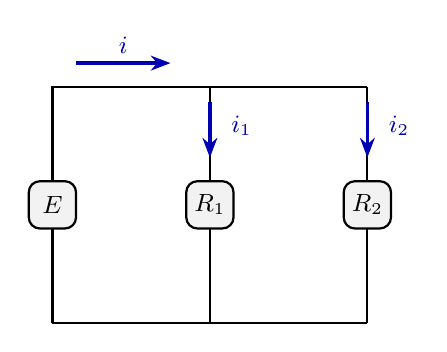
\begin{tikzpicture}[scale=1.0]
  \draw[thick] (0,0) -- (0,3) -- (4,3);
  \draw[thick, fill=gray!10, rounded corners] (-0.3,1.2) rectangle (0.3,1.8);
  \node[font=\small] at (0,1.5) {$E$};
  \draw[thick] (2,3) -- (2,0);
  \draw[thick, fill=gray!10, rounded corners] (1.7,1.2) rectangle (2.3,1.8);
  \node[font=\small] at (2,1.5) {$R_1$};
  \draw[thick] (4,3) -- (4,0);
  \draw[thick, fill=gray!10, rounded corners] (3.7,1.2) rectangle (4.3,1.8);
  \node[font=\small] at (4,1.5) {$R_2$};
  \draw[thick] (0,0) -- (4,0);
  
  \draw[line width=1.3pt, blue!70!black, -{Stealth[length=2.5mm]}] (0.3,3.3) -- (1.5,3.3);
  \node[blue!70!black, above, font=\small] at (0.9,3.3) {$i$};
  \draw[line width=1.3pt, blue!70!black, -{Stealth[length=2.5mm]}] (2,2.8) -- (2,2.1);
  \node[blue!70!black, right, font=\small] at (2.15,2.5) {$i_1$};
  \draw[line width=1.3pt, blue!70!black, -{Stealth[length=2.5mm]}] (4,2.8) -- (4,2.1);
  \node[blue!70!black, right, font=\small] at (4.15,2.5) {$i_2$};
\end{tikzpicture}
\end{center}

\textbf{Résolution :}

\textit{KCL} (n\oe ud haut) : $i = i_1 + i_2$.

\textit{KVL} ($R_1$ et $R_2$ en parallèle $\Rightarrow$ même tension $E$) :
$i_1 = E/R_1 = 12/4 = \SI{3}{A}$, \quad $i_2 = E/R_2 = 12/6 = \SI{2}{A}$, \quad $i = \SI{5}{A}$.

\textit{Bilan :} $P_E = 12 \times 5 = \SI{60}{W}$. $P_1 = 4\times9 = \SI{36}{W}$. $P_2 = 6\times4 = \SI{24}{W}$. Total : $36+24 = \SI{60}{W}$. \checkmark

\subsection{Le diviseur de courant}

Le diviseur de courant est le \textbf{dual} du diviseur de tension (chapitre 3). Quand un courant $i$ se partage entre deux résistances en parallèle $R_1$ et $R_2$ :

\begin{formule}
\[
\boxed{i_1 = i \cdot \frac{R_2}{R_1 + R_2}} \qquad \boxed{i_2 = i \cdot \frac{R_1}{R_1 + R_2}}
\]
Chaque branche reçoit une fraction du courant total, inversement proportionnelle à sa résistance.
\end{formule}

\begin{intuition}
C'est logique : le courant ``préfère'' le chemin le plus facile (la résistance la plus faible). Si $R_1 \ll R_2$, presque tout le courant passe dans $R_1$.

Moyen mnémotechnique : dans la formule de $i_1$, c'est $R_2$ qui apparaît au numérateur (\textit{l'autre} résistance). C'est l'inverse du diviseur de tension.
\end{intuition}

\textbf{Vérification avec l'exemple précédent :} $i_1 = 5 \times 6/(4+6) = 5 \times 0{,}6 = \SI{3}{A}$. \checkmark

\subsection{Exemple avec deux sources de tension}

Ce cas est le premier où Kirchhoff devient \textit{vraiment indispensable} : deux générateurs se ``combattent'' et on ne peut pas résoudre par de simples séries/parallèles.

\textbf{Énoncé :} $E_1 = \SI{12}{V}$, $E_2 = \SI{8}{V}$, $R_1 = \SI{2}{\ohm}$, $R_2 = \SI{4}{\ohm}$, $R_3 = \SI{6}{\ohm}$.

\begin{center}
\begin{circuitikz}[scale=0.85]
  \draw (0,0) to[battery1, l=$E_1$, invert] (0,3)
        to[R, l=$R_1$] (3,3)
        to[R, l=$R_3$] (3,0) -- (0,0);
  \draw (3,3) to[R, l=$R_2$] (6,3)
        to[battery1, l=$E_2$] (6,0) -- (3,0);
  \draw[line width=1.2pt, blue!70!black, -{Stealth[length=2.5mm]}] (0.3,2.7) -- (1.2,2.7);
  \node[blue!70!black, above, font=\small] at (0.75,2.7) {$i_1$};
  \draw[line width=1.2pt, blue!70!black, -{Stealth[length=2.5mm]}] (3,2.7) -- (3,1.9);
  \node[blue!70!black, right, font=\small] at (3.1,2.3) {$i_3$};
  \draw[line width=1.2pt, blue!70!black, -{Stealth[length=2.5mm]}] (3.5,2.7) -- (4.5,2.7);
  \node[blue!70!black, above, font=\small] at (4,2.7) {$i_2$};
\end{circuitikz}
\end{center}

\textbf{Résolution (Kirchhoff direct) :}

\textit{KCL} au n\oe ud central (haut-droit) : $i_1 = i_2 + i_3$ \quad (1)

\textit{KVL maille gauche} (sens horaire) : $E_1 - R_1 i_1 - R_3 i_3 = 0 \Rightarrow 12 - 2i_1 - 6i_3 = 0$ \quad (2)

\textit{KVL maille droite} (sens horaire) : $R_3 i_3 - R_2 i_2 - E_2 = 0 \Rightarrow 6i_3 - 4i_2 - 8 = 0$ \quad (3)

Substituons (1) dans (2) : $12 - 2(i_2 + i_3) - 6i_3 = 0 \Rightarrow 12 - 2i_2 - 8i_3 = 0$ \quad (2')

De (3) : $i_2 = (6i_3 - 8)/4$. Dans (2') :
$12 - 2(6i_3-8)/4 - 8i_3 = 0 \Rightarrow 12 - 3i_3 + 4 - 8i_3 = 0 \Rightarrow 16 = 11i_3$

$i_3 = 16/11 \approx \SI{1.45}{A}$

$i_2 = (6\times1{,}45 - 8)/4 = 0{,}73/4 \approx \SI{0.18}{A}$

$i_1 = i_2 + i_3 = 0{,}18 + 1{,}45 = \SI{1.64}{A}$

\textit{Bilan de puissance :}
\begin{itemize}[nosep]
\item $P_{E_1} = E_1 i_1 = 12\times1{,}64 = \SI{19.6}{W}$ (fournie)
\item $P_{E_2} = E_2 i_2 = 8\times0{,}18 = \SI{1.5}{W}$ ($i_2$ \textit{entre} par le $+$ de $E_2$ : elle \textit{reçoit} de l'énergie, comme une batterie en charge !)
\item $P_{R_1} = 2\times1{,}64^2 = \SI{5.4}{W}$, $P_{R_2} = 4\times0{,}18^2 = \SI{0.1}{W}$, $P_{R_3} = 6\times1{,}45^2 = \SI{12.7}{W}$
\item Total dissipé + reçu : $5{,}4+0{,}1+12{,}7+1{,}5 = \SI{19.7}{W} \approx P_{E_1}$. \checkmark
\end{itemize}

\begin{attention}
\textbf{Observation importante :} $E_2$ ne fournit pas de courant dans cet exemple --- elle en \textit{reçoit}. C'est le cas typique d'une batterie en charge. Le signe du résultat nous l'a révélé automatiquement. C'est la puissance du formalisme algébrique de Kirchhoff : on pose, on calcule, les signes parlent.
\end{attention}

\subsection{Les erreurs classiques}

\begin{attention}
\textbf{Les 5 pièges les plus fréquents avec Kirchhoff :}

\textbf{1. Oublier de définir un sens pour chaque courant.} On \textit{doit} choisir un sens (même arbitraire) avant d'écrire la moindre équation. Sans convention, les signes n'ont aucun sens.

\textbf{2. Confondre le sens choisi et le sens réel.} Le sens choisi est une hypothèse. Si le résultat est négatif, le courant réel va en sens inverse. Ce n'est \textit{jamais} une erreur --- c'est le fonctionnement normal.

\textbf{3. Se tromper de signe dans la KVL.} Règle : en parcourant une maille, si l'on entre par le $+$ d'un composant et sort par le $-$, sa tension est comptée $+$ dans le sens du parcours. Inversement : $-$.

\textbf{4. Écrire trop d'équations.} Si on écrit $n$ lois des n\oe uds au lieu de $n-1$, la dernière est redondante et le système est indéterminé. Il faut exactement $n-1$ KCL et $b-n+1$ KVL.

\textbf{5. Oublier le bilan de puissance.} C'est la seule vérification fiable. Si $\sum P_{\text{fournie}} \neq \sum P_{\text{dissipée}}$, il y a une erreur quelque part.
\end{attention}

\begin{retenir}
\textbf{Les 2 lois de Kirchhoff :}
\begin{enumerate}[nosep]
\item \textbf{KCL} : $\sum i_k = 0$ en tout n\oe ud $\longleftrightarrow$ conservation de la charge.
\item \textbf{KVL} : $\sum U_k = 0$ sur toute maille $\longleftrightarrow$ conservation de l'énergie.
\end{enumerate}
Ces deux lois + la loi d'Ohm suffisent à résoudre tout circuit linéaire.

\textbf{Attention :} ces lois reposent sur une hypothèse implicite (l'ARQS) qui sera précisée dans la section Niveau Ingénieur. En basse fréquence et sur des circuits de taille raisonnable, elles sont \textit{toujours} valides.
\end{retenir}

% ----------------------------------------------------------------------------
% SECTION 2 : APPROFONDISSEMENT
% ----------------------------------------------------------------------------
\section{Approfondissement}

\begin{approfondissement}
Méthodes systématiques de résolution : courants de maille et potentiels de n\oe uds. Prérequis : systèmes d'équations linéaires.
\end{approfondissement}

\subsection{Combien d'équations écrire ?}

Pour un circuit plan à $b$ branches et $n$ n\oe uds :
\begin{itemize}[nosep]
\item Équations KCL indépendantes : $n - 1$ (on en ``oublie'' un, car la dernière est combinaison des autres).
\item Équations KVL indépendantes : $m = b - n + 1$ (nombre de mailles indépendantes).
\item Total : $(n-1) + (b-n+1) = b$ équations pour $b$ inconnues (les courants de branche).
\end{itemize}

\subsection{Méthode des courants de maille}

On définit un \textbf{courant fictif} circulant dans chaque maille indépendante. Le courant réel dans une branche est la somme algébrique des courants de maille qui la traversent.

\textbf{Avantage :} la KCL est automatiquement vérifiée. On n'écrit que des KVL.

\textbf{Exemple :} $E = \SI{10}{V}$, $R_1 = \SI{2}{\ohm}$, $R_2 = \SI{3}{\ohm}$ (branche commune), $R_3 = \SI{5}{\ohm}$.

\begin{center}
\begin{circuitikz}[scale=0.85]
  \draw (0,0) to[battery1, l=$E$, invert] (0,3)
        to[R, l=$R_1$] (3,3)
        to[R, l=$R_2$] (3,0) -- (0,0);
  \draw (3,3) to[R, l=$R_3$] (6,3) -- (6,0) -- (3,0);
  \draw[-{Stealth[length=2.5mm]}, blue!60!black, thick] (1.5,1.2) arc[start angle=180, end angle=-120, radius=0.5];
  \node[blue!60!black] at (1.5,1.5) {$I_a$};
  \draw[-{Stealth[length=2.5mm]}, green!60!black, thick] (4.5,1.2) arc[start angle=180, end angle=-120, radius=0.5];
  \node[green!60!black] at (4.5,1.5) {$I_b$};
\end{circuitikz}
\end{center}

Maille $a$ : $(R_1 + R_2)I_a - R_2 I_b = E \Rightarrow 5I_a - 3I_b = 10$ \quad (1)

Maille $b$ : $-R_2 I_a + (R_2 + R_3)I_b = 0 \Rightarrow -3I_a + 8I_b = 0$ \quad (2)

De (2) : $I_a = 8I_b/3$. Dans (1) : $40I_b/3 - 3I_b = 10 \Rightarrow 31I_b/3 = 10 \Rightarrow I_b = 30/31 \approx \SI{0.968}{A}$.

$I_a = 8 \times 0{,}968/3 \approx \SI{2.58}{A}$. Courant dans $R_2$ : $I_a - I_b \approx \SI{1.61}{A}$.

\subsection{Méthode des potentiels de n\oe uds}

On choisit un n\oe ud de référence (masse, $V = 0$), et on écrit les potentiels des autres n\oe uds comme inconnues. On applique la KCL en exprimant les courants via $i = (V_A - V_B)/R$.

\textbf{Avantage :} la KVL est automatiquement vérifiée. Le nombre d'inconnues est $n - 1$.

\textbf{Exemple résolu :} reprenons le circuit de la section précédente : $E = \SI{10}{V}$, $R_1 = \SI{2}{\ohm}$, $R_2 = \SI{3}{\ohm}$, $R_3 = \SI{5}{\ohm}$ (même topologie que l'exemple des courants de maille).

\begin{enumerate}[nosep]
\item \textbf{Choix de la masse :} n\oe ud du bas.
\item \textbf{Inconnues :} 2 n\oe uds (haut-gauche = A, haut-droite = B). $V_A$ est imposé par la source : $V_A = E = \SI{10}{V}$. Il reste une seule inconnue : $V_B$.
\item \textbf{KCL au n\oe ud B :} le courant arrivant par $R_1$ + le courant arrivant par $R_3$ = le courant partant par $R_2$ :
\[
\frac{V_A - V_B}{R_1} + \frac{0 - V_B}{R_3} = \frac{V_B - 0}{R_2} \quad \text{(attention : ici } R_3 \text{ va de B à la masse)}
\]
Attendons --- vérifions la topologie sur le schéma : $E$ alimente $R_1$, puis au n\oe ud B on a $R_2$ et $R_3$ qui vont chacune vers la masse (c'est $R_1$ en série avec $R_2 \parallel R_3$). Donc :
\[
\frac{V_A - V_B}{R_1} = \frac{V_B}{R_2} + \frac{V_B}{R_3}
\]
\[
\frac{10 - V_B}{2} = V_B\left(\frac{1}{3} + \frac{1}{5}\right) = \frac{8\,V_B}{15}
\]
En multipliant par 30 : $15(10-V_B) = 16V_B \Rightarrow 150 = 31V_B \Rightarrow V_B = 150/31 \approx \SI{4.84}{V}$.
\end{enumerate}

Vérification : $i_{R_1} = (10-4{,}84)/2 = \SI{2.58}{A}$, $i_{R_2} = 4{,}84/3 = \SI{1.61}{A}$, $i_{R_3} = 4{,}84/5 = \SI{0.968}{A}$.

KCL en B : $2{,}58 = 1{,}61 + 0{,}97 = 2{,}58$. \checkmark{} --- et les valeurs sont identiques à celles trouvées par les courants de maille.

\begin{pratique}
\textbf{Quelle méthode choisir ?}
\begin{itemize}[nosep]
\item \textbf{Courants de maille :} peu de mailles, beaucoup de n\oe uds, sources de tension.
\item \textbf{Potentiels de n\oe uds :} peu de n\oe uds, beaucoup de mailles, sources de courant.
\item Les \textbf{simulateurs} (SPICE) utilisent les potentiels de n\oe uds (méthode MNA) car la mise en matrice est systématique.
\end{itemize}
\end{pratique}

\subsection{Écriture matricielle}

Les deux méthodes se mettent sous forme d'un système linéaire :
\begin{formule}
\[
\boxed{[G] \cdot [V] = [I]}
\]
$[G]$ : matrice de conductance (symétrique pour circuits passifs), $[V]$ : potentiels, $[I]$ : sources. C'est exactement ce que SPICE construit et résout.
\end{formule}

\subsection{Kirchhoff en régime variable (AC, transitoire)}

Les lois de Kirchhoff restent valables en régime variable \textbf{tant que l'ARQS est vérifiée} :
\begin{itemize}[nosep]
\item KCL : s'applique avec les courants instantanés $i(t)$.
\item KVL : s'applique en incluant $u_C = q/C$ et $u_L = L\,\mathrm{d}i/\mathrm{d}t$ comme tensions de dipôles.
\end{itemize}

En régime sinusoïdal permanent, on peut simplifier considérablement les calculs en utilisant les \textbf{nombres complexes}. L'idée (qui sera développée au chapitre 10) est de remplacer les fonctions sinusoïdales par des exponentielles complexes. Chaque composant est alors caractérisé par une \textbf{impédance complexe} $\underline{Z}$ qui généralise la résistance :
\[
\underline{Z}_R = R, \qquad \underline{Z}_C = \frac{1}{j\omega C}, \qquad \underline{Z}_L = j\omega L
\]
où $j^2 = -1$ et $\omega = 2\pi f$ est la pulsation.

Les lois de Kirchhoff gardent \textbf{exactement la même forme} avec des tensions et courants complexes $\underline{U}$ et $\underline{I}$ :
\[
\sum \underline{I}_k = 0 \quad \text{(KCL)} \qquad\qquad \sum \underline{U}_k = 0 \quad \text{(KVL)}
\]

\begin{intuition}
On n'a pas besoin de réapprendre Kirchhoff pour l'alternatif. Il suffit de remplacer $R$ par $\underline{Z}$ dans toutes les formules. C'est la grande puissance de la notation complexe : elle transforme des équations différentielles en simples équations algébriques.

\textit{Un rappel mathématique complet sur les nombres complexes sera donné au début du chapitre 10.}
\end{intuition}

% ----------------------------------------------------------------------------
% SECTION 3 : NIVEAU INGÉNIEUR
% ----------------------------------------------------------------------------
\section{Niveau Ingénieur}

\begin{ingenieur}
Fondements électromagnétiques des lois de Kirchhoff, domaine de validité exact, et conséquences en conception réelle.
\end{ingenieur}

\subsection{Fondement électromagnétique : d'où viennent les lois de Kirchhoff ?}

Les lois de Kirchhoff ne sont \textit{pas} des lois fondamentales de la physique. Ce sont des \textbf{approximations} des équations de Maxwell, valides sous l'hypothèse ARQS ($d \ll \lambda$).

\textbf{KCL $\leftarrow$ Conservation de la charge} (équation de continuité) :
\[
\nabla \cdot \vec{J} = -\frac{\partial \rho}{\partial t}
\]
En ARQS, $\partial\rho/\partial t \approx 0$ en tout point du circuit, donc $\nabla\cdot\vec{J} = 0$. En intégrant sur un volume entourant un n\oe ud : $\oint_S \vec{J}\cdot\mathrm{d}\vec{S} = 0$, ce qui donne $\sum i_k = 0$.

\textbf{KVL $\leftarrow$ Équation de Maxwell-Faraday} :
\[
\oint_{\mathcal{C}} \vec{E}\cdot\mathrm{d}\vec{\ell} = -\frac{\mathrm{d}\Phi_B}{\mathrm{d}t}
\]
En ARQS, si le flux magnétique intercepté par la maille est négligeable : $\oint \vec{E}\cdot\mathrm{d}\vec{\ell} \approx 0$. Les ``tensions'' aux bornes des composants sont les intégrales de $\vec{E}$ sur chaque segment, et leur somme est nulle. C'est la KVL.

\begin{attention}
\textbf{Quand KVL échoue :} la loi des mailles n'est plus valable quand le flux magnétique $\Phi_B$ à travers la maille varie significativement. Cela se produit dans :
\begin{itemize}[nosep]
\item Les \textbf{transformateurs} et bobines couplées (couplage magnétique voulu).
\item Les \textbf{boucles de masse} sur PCB proches de conducteurs de puissance (couplage parasite).
\item Les circuits dont les dimensions approchent $\lambda/10$.
\end{itemize}
\textbf{Solution :} on modélise le flux parasite par une inductance mutuelle $M$ ou une f.é.m.\ induite $e = -\mathrm{d}\Phi_B/\mathrm{d}t$ qu'on \textit{inclut} dans la maille. La KVL ``étendue'' reste alors utilisable.
\end{attention}

\begin{attention}
\textbf{Piège fondamental :} les lois de Kirchhoff sont si naturelles et si systématiquement enseignées que beaucoup d'ingénieurs oublient qu'elles ont un \textbf{domaine de validité limité}. En haute fréquence ou sur des circuits de grande dimension, il faut passer aux \textbf{lignes de transmission} (équations des télégraphistes) ou aux \textbf{équations de Maxwell complètes}. Règle pratique : si $d > \lambda/10$, Kirchhoff est suspect.
\end{attention}

\subsection{SPICE et la Modified Nodal Analysis (MNA)}

Les simulateurs de circuits utilisent la \textbf{MNA}, extension de la méthode des potentiels de n\oe uds :

\begin{enumerate}[nosep]
\item Construction de la matrice $[G][V] = [I]$ depuis la netlist.
\item \textbf{DC :} résolution directe (linéaire) ou Newton-Raphson (non-linéaire).
\item \textbf{AC :} $R \to \underline{Z}(\omega)$, résolution pour chaque fréquence.
\item \textbf{Transitoire :} discrétisation temporelle, résolution à chaque pas de temps.
\end{enumerate}

Comprendre Kirchhoff et la méthode des potentiels de n\oe uds, c'est comprendre \textit{exactement} ce que fait SPICE.

\subsection{Pièges en conception réelle}

\begin{pratique}
\textbf{1. Les fils ne sont pas idéaux.} Chaque piste, via ou bonding wire a une résistance et une inductance parasites. La chute de tension $V = L\,\mathrm{d}i/\mathrm{d}t$ dans une piste de masse est une source majeure de problèmes (\textit{ground bounce}).

\textbf{2. La masse n'est pas un point.} ``GND'' sur un PCB est un plan de cuivre avec une impédance distribuée. Si deux circuits partagent un chemin de retour, leurs courants créent des chutes de tension parasites (problème des \textit{ground loops}).

\textbf{3. Règles de conception :}
\begin{itemize}[nosep]
\item Plans de masse continus et ininterrompus.
\item Condensateurs de découplage (\SI{100}{nF}) au plus près de chaque CI.
\item Séparation des retours de courant (analogique / numérique / puissance).
\item Si nécessaire : connexion en étoile (\textit{star ground}).
\end{itemize}
\end{pratique}

% === EXERCICES DU CHAPITRE 5 ===
\section*{Exercices}
\addcontentsline{toc}{section}{Exercices}

\subsection*{Niveau débutant}

\textbf{Exercice 5.1 ---} En un n\oe ud arrivent trois courants : $i_1 = \SI{3}{A}$ (entrant), $i_2 = \SI{-1}{A}$ (sortant), $i_3$ inconnu. Déterminez $i_3$.

\begin{pratique}
\textbf{Solution :} $i_1 + i_2 + i_3 = 0 \Rightarrow 3 + (-1) + i_3 = 0 \Rightarrow i_3 = \SI{-2}{A}$ (sort du n\oe ud).
\end{pratique}

\textbf{Exercice 5.2 ---} Circuit série : $E = \SI{15}{V}$, $R_1 = \SI{100}{\ohm}$, $R_2 = \SI{220}{\ohm}$, $R_3 = \SI{330}{\ohm}$. Calculez $I$ et les tensions. Vérifiez la KVL.

\begin{pratique}
\textbf{Solution :} $I = E/(R_1+R_2+R_3) = 15/650 = \SI{23.1}{mA}$.

$U_1 = \SI{2.31}{V}$, $U_2 = \SI{5.08}{V}$, $U_3 = \SI{7.62}{V}$.

KVL : $2{,}31+5{,}08+7{,}62 = \SI{15.01}{V} \approx E$. \checkmark
\end{pratique}

\subsection*{Niveau intermédiaire}

\textbf{Exercice 5.3 ---} Deux sources : $E_1 = \SI{10}{V}$, $E_2 = \SI{6}{V}$, $R_1 = \SI{2}{\ohm}$, $R_2 = \SI{4}{\ohm}$ (branche commune), $R_3 = \SI{3}{\ohm}$. Résolvez par les courants de maille.

\begin{pratique}
\textbf{Solution :} Maille $a$ : $(R_1+R_2)I_a - R_2 I_b = E_1 \Rightarrow 6I_a - 4I_b = 10$ \quad (1)

Maille $b$ : $-R_2 I_a + (R_2+R_3)I_b = -E_2 \Rightarrow -4I_a + 7I_b = -6$ \quad (2)

De (2) : $I_a = (7I_b + 6)/4$. Dans (1) : $6(7I_b+6)/4 - 4I_b = 10$

$42I_b/4 + 36/4 - 4I_b = 10 \Rightarrow 10{,}5I_b + 9 - 4I_b = 10 \Rightarrow 6{,}5I_b = 1$

$I_b = \SI{0.154}{A}$. $I_a = (7\times0{,}154+6)/4 = \SI{1.77}{A}$. $I_{R_2} = I_a - I_b = \SI{1.62}{A}$.
\end{pratique}

\textbf{Exercice 5.4 ---} Un circuit a 4 n\oe uds et 6 branches. Combien d'équations KCL et KVL indépendantes ? Avec la méthode des potentiels de n\oe uds, combien d'inconnues ?

\begin{pratique}
\textbf{Solution :} KCL : $n-1 = 3$. KVL : $b-n+1 = 6-4+1 = 3$. Total : $3+3 = 6 = b$. \checkmark

Potentiels de n\oe uds : $n-1 = 3$ inconnues (les 3 potentiels des n\oe uds non référencés).
\end{pratique}

\subsection*{Niveau ingénieur}

\textbf{Exercice 5.5 ---} Un CI numérique commute \SI{1}{A} en \SI{1}{ns} ($\mathrm{d}i/\mathrm{d}t = \SI{e9}{A/s}$). L'inductance parasite de la piste de masse est \SI{5}{nH}. Calculez la tension de \textit{ground bounce}. Conséquences ?

\begin{pratique}
\textbf{Solution :} $V = L\,\mathrm{d}i/\mathrm{d}t = 5\times10^{-9} \times 10^{9} = \SI{5}{V}$.

\textbf{5 V de bruit sur la masse !} Catastrophique pour un circuit analogique voisin travaillant au mV. Solutions : plans de masse continus, découplage \SI{100}{nF} au plus près, séparation des retours de courant.
\end{pratique}

\textbf{Exercice 5.6 ---} Un signal à \SI{500}{MHz} circule sur un PCB de \SI{15}{cm}. Vitesse de propagation dans le FR-4 : $\sim\SI{1.5e8}{m/s}$. Kirchhoff est-il applicable ?

\begin{pratique}
\textbf{Solution :} $\lambda = c/f = 1{,}5\times10^8 / 5\times10^8 = \SI{0.30}{m} = \SI{30}{cm}$.

$d/\lambda = 15/30 = 0{,}5$. Or la limite est $d < \lambda/10 = \SI{3}{cm}$.

Kirchhoff est \textbf{totalement inapplicable}. Il faut utiliser les \textbf{lignes de transmission} (impédance caractéristique, adaptation, réflexions).
\end{pratique}

\subsection*{Questions de compréhension}

\begin{enumerate}[nosep]
\item Pourquoi dit-on que les lois de Kirchhoff ``contiennent'' implicitement la loi d'Ohm ?
\item Un circuit série $R$-$L$ est alimenté par une tension sinusoïdale. La KVL est-elle applicable ? Comment inclut-on la tension de la bobine ?
\item Expliquez pourquoi un condensateur de découplage de \SI{100}{nF} placé au plus près d'un CI réduit le \textit{ground bounce}.
\item Si un voltmètre mesure une tension différente selon la position de ses fils de mesure (alors qu'il est branché entre les deux mêmes points), que peut-on en conclure sur la validité de la KVL dans cette situation ?
\end{enumerate}

% === RÉSUMÉ DU CHAPITRE 5 ===
\section*{Résumé du chapitre}
\addcontentsline{toc}{section}{Résumé du chapitre}

\begin{bases}[title={\color{white} Résumé --- Les Bases}]
\begin{center}
\renewcommand{\arraystretch}{1.3}
\begin{tabular}{p{4.5cm}p{8.5cm}}
\toprule
KCL (loi des n\oe uds) & $\sum i_k = 0$ en tout n\oe ud --- conservation de la charge \\
KVL (loi des mailles) & $\sum U_k = 0$ sur toute maille --- conservation de l'énergie \\
Diviseur de courant & $i_1 = i \cdot R_2/(R_1+R_2)$ --- dual du diviseur de tension \\
\bottomrule
\end{tabular}
\end{center}
\end{bases}

\begin{approfondissement}[title={\color{white} Résumé --- Approfondissement}]
\begin{center}
\renewcommand{\arraystretch}{1.3}
\begin{tabular}{p{4.5cm}p{8.5cm}}
\toprule
Nombre d'équations & $b$ branches, $n$ n\oe uds $\Rightarrow$ $b$ équations indépendantes \\
Courants de maille & Méthode systématique, KCL automatique \\
Potentiels de n\oe uds & Méthode systématique, KVL automatique, base de SPICE \\
Impédances (aperçu) & $\underline{Z}_R = R$, $\underline{Z}_C = 1/j\omega C$, $\underline{Z}_L = j\omega L$ \\
\bottomrule
\end{tabular}
\end{center}
\end{approfondissement}

\begin{ingenieur}[title={\color{white} Résumé --- Niveau Ingénieur}]
\begin{center}
\renewcommand{\arraystretch}{1.3}
\begin{tabular}{p{4.5cm}p{8.5cm}}
\toprule
Fondement Maxwell & KCL $\leftarrow$ $\nabla\cdot\vec{J}=0$ ; KVL $\leftarrow$ $\oint\vec{E}\cdot\mathrm{d}\vec{\ell} \approx 0$ \\
Validité (ARQS) & $d \ll \lambda/10$ ; au-delà $\to$ lignes de transmission \\
En pratique & Fils $\neq$ idéaux, masse $\neq$ équipotentielle, ground bounce \\
\bottomrule
\end{tabular}
\end{center}
\end{ingenieur}


% ============================================================================
% CHAPITRE 6 : THÉORÈMES FONDAMENTAUX
% ============================================================================
\chapter{Théorèmes Fondamentaux}

\begin{center}
\textit{Superposition, Thévenin, Norton, Millman :\\
quatre outils pour simplifier n'importe quel circuit linéaire\\
sans écrire le système complet de Kirchhoff.}
\end{center}

\vspace{0.3cm}

Au chapitre 5, nous avons vu que les lois de Kirchhoff permettent de résoudre tout circuit --- mais au prix d'un système de $b$ équations à $b$ inconnues. Pour un circuit à 10 branches, c'est 10 équations. Les théorèmes de ce chapitre permettent de \textbf{raccourcir le travail} en exploitant les propriétés des circuits linéaires.

% ----------------------------------------------------------------------------
% SECTION 1 : LES BASES
% ----------------------------------------------------------------------------
\section{Les Bases}

\begin{bases}
Cette section présente les quatre théorèmes de manière intuitive, avec des exemples concrets. Prérequis : chapitres 1 à 5.
\end{bases}

\subsection{Qu'est-ce qu'un circuit linéaire ?}

Tous les théorèmes de ce chapitre ne s'appliquent qu'aux \textbf{circuits linéaires}. Un circuit est linéaire si tous ses composants obéissent à des relations linéaires entre tension et courant : résistances ($U = RI$), condensateurs ($i = C\,\mathrm{d}u/\mathrm{d}t$), inductances ($u = L\,\mathrm{d}i/\mathrm{d}t$), sources indépendantes et sources dépendantes linéaires.

\begin{attention}
Les diodes, transistors (en grand signal), et tout composant dont la relation entre tension et courant n'obéit pas au \textbf{principe de proportionnalité et d'additivité} ne sont pas linéaires. Les théorèmes de ce chapitre ne s'appliquent pas directement à ces composants. On peut cependant les utiliser sur le \textit{modèle petit signal} linéarisé autour d'un point de fonctionnement (cf.\ chapitres sur les semi-conducteurs).

\begin{attention}
\textbf{Linéaire $\neq$ ``droite $I(U)$''.} Un condensateur ($i = C\,\mathrm{d}u/\mathrm{d}t$) et une inductance ($u = L\,\mathrm{d}i/\mathrm{d}t$) \textit{sont} des composants linéaires, même si leur relation $I(U)$ n'est pas une simple droite. Ce qui compte, c'est que la relation entre entrée et sortie vérifie : si l'on double la tension, le courant double. C'est la définition mathématique de la linéarité (opérateur linéaire), pas la forme géométrique de la caractéristique statique.
\end{attention}
\end{attention}

\subsection{Théorème de superposition}

\begin{formule}
\textbf{Théorème de superposition :} dans un circuit linéaire contenant plusieurs sources indépendantes, la réponse (tension ou courant) en tout point est la \textbf{somme} des réponses obtenues en considérant chaque source \textit{seule}, les autres étant ``éteintes'' :
\begin{itemize}[nosep]
\item Source de tension éteinte $\rightarrow$ remplacée par un \textbf{court-circuit} (fil).
\item Source de courant éteinte $\rightarrow$ remplacée par un \textbf{circuit ouvert} (coupure).
\end{itemize}
\end{formule}

\begin{intuition}
L'idée est simple : dans un circuit linéaire, chaque source ``pousse'' indépendamment les courants et tensions. L'effet total est la somme des effets individuels. C'est comme la houle sur la mer : deux vagues se superposent sans s'influencer mutuellement.
\end{intuition}

\textbf{Exemple :} circuit avec $E_1 = \SI{12}{V}$, $E_2 = \SI{6}{V}$, $R_1 = \SI{4}{\ohm}$, $R_2 = \SI{2}{\ohm}$. On cherche le courant dans $R_2$.

\begin{center}
\begin{circuitikz}[scale=0.8]
  \draw (0,0) to[battery1, l=$E_1$, invert] (0,3) to[R, l=$R_1$] (3,3) to[R, l=$R_2$] (3,0) -- (0,0);
  \draw (3,3) -- (5,3) to[battery1, l=$E_2$] (5,0) -- (3,0);
\end{circuitikz}
\end{center}

\textit{Étape 1 :} $E_1$ seule ($E_2$ court-circuitée). $R_1$ et $R_2$ sont en série, $R_2$ est en parallèle avec le court-circuit de $E_2$... Non : $E_2$ court-circuitée met les bornes de $R_2$ en parallèle avec le fil. Donc $R_2$ est court-circuitée aussi !

$i'_{R_2} = 0$ (tout le courant passe par le court-circuit de $E_2$, pas par $R_2$).

Reprenons : en fait, $R_2$ est entre le n\oe ud haut et le bas. $E_2$ court-circuitée = fil entre le n\oe ud haut-droit et le bas. Donc $R_2$ est en parallèle avec un fil $\Rightarrow$ court-circuit $\Rightarrow i'_{R_2} = 0$.

\textit{Étape 2 :} $E_2$ seule ($E_1$ court-circuitée). Même raisonnement : $R_1$ est court-circuitée par le fil de $E_1$. Le courant dans $R_2$ vaut $i''_{R_2} = E_2/R_2 = 6/2 = \SI{3}{A}$.

\textit{Résultat :} $i_{R_2} = i'_{R_2} + i''_{R_2} = 0 + 3 = \SI{3}{A}$.

\begin{attention}
\textbf{Piège classique :} la superposition s'applique aux \textbf{courants et tensions}, mais \textit{pas} à la puissance ! La puissance dépend du carré du courant ($P = RI^2$), ce qui n'est pas une opération linéaire. On ne peut pas additionner les puissances partielles.

\textbf{Sources dépendantes :} seules les sources \textit{indépendantes} sont éteintes une à une. Les sources \textit{dépendantes} (commandées par une grandeur du circuit) restent \textbf{toujours actives} --- elles font partie intégrante du circuit, pas des excitations. Ce point est détaillé dans la section Approfondissement.
\end{attention}

\subsection{Théorème de Thévenin}

C'est probablement le théorème \textbf{le plus utile} de toute l'électronique.

\begin{formule}
\textbf{Théorème de Thévenin :} tout circuit linéaire, vu depuis deux bornes A et B, peut être remplacé par un \textbf{générateur de Thévenin} constitué de :
\begin{itemize}[nosep]
\item une source de tension $E_{\text{th}}$ (tension à vide entre A et B),
\item en série avec une résistance $R_{\text{th}}$ (résistance vue entre A et B quand toutes les sources indépendantes sont éteintes).
\end{itemize}

\begin{center}
\begin{circuitikz}[scale=0.9]
  \draw (0,0) to[battery1, l=$E_{\text{th}}$, invert] (0,2)
        to[R, l=$R_{\text{th}}$] (3,2) node[right]{A};
  \draw (0,0) -- (3,0) node[right]{B};
\end{circuitikz}
\end{center}
\end{formule}

\begin{intuition}
Imaginez un appareil électronique complexe (un amplificateur, une alimentation, un capteur\ldots) avec deux fils de sortie. Vu de l'extérieur, peu importe ce qu'il y a dedans : tout ce que la charge ``voit'', c'est une tension à vide $E_{\text{th}}$ qui chute quand on tire du courant, à cause d'une résistance interne $R_{\text{th}}$. C'est exactement le modèle du générateur réel du chapitre 2 !

\textbf{Attention :} l'équivalent de Thévenin n'est \textit{pas} une propriété intrinsèque du circuit. Il \textbf{dépend des bornes choisies}. Si vous changez de bornes (par exemple, vous regardez entre deux autres points), $E_{\text{th}}$ et $R_{\text{th}}$ changent. Un même circuit a autant d'équivalents de Thévenin que de paires de bornes.
\end{intuition}

\textbf{Comment trouver $E_{\text{th}}$ et $R_{\text{th}}$ :}

\begin{enumerate}
\item \textbf{$E_{\text{th}}$} = tension entre A et B \textit{à vide} (rien de branché entre A et B). On calcule $V_A - V_B$ avec les méthodes habituelles.
\item \textbf{$R_{\text{th}}$} = résistance vue entre A et B après avoir éteint toutes les sources indépendantes. On ``regarde'' le circuit depuis A et B, et on calcule la résistance équivalente.
\end{enumerate}

\textbf{Exemple :} trouver l'équivalent de Thévenin vu de A-B.

\begin{center}
\begin{circuitikz}[scale=0.85]
  \draw (0,0) to[battery1, l=$E{=}\SI{12}{V}$, invert] (0,3)
        to[R, l=$R_1{=}\SI{6}{\ohm}$] (3,3);
  \draw (3,3) -- (3,2) to[R, l=$R_2{=}\SI{3}{\ohm}$] (3,0);
  \draw (0,0) -- (3,0);
  \filldraw[blue!70!black] (3,3) circle (2pt);
  \node[right, font=\bfseries] at (3.2,3) {A};
  \filldraw[blue!70!black] (3,0) circle (2pt);
  \node[right, font=\bfseries] at (3.2,0) {B};
\end{circuitikz}
\end{center}

\textit{$E_{\text{th}}$} : à vide, pas de courant dans $R_1$ (car rien n'est branché entre A et B, et $R_2$ est en parallèle avec la sortie). En fait, $R_1$ et $R_2$ forment un diviseur de tension :
\[
E_{\text{th}} = E \cdot \frac{R_2}{R_1 + R_2} = 12 \times \frac{3}{6+3} = \SI{4}{V}
\]

\textit{$R_{\text{th}}$} : on éteint $E$ (court-circuit). Vu de A-B, $R_1$ et $R_2$ sont en parallèle :
\[
R_{\text{th}} = R_1 \parallel R_2 = \frac{6 \times 3}{6 + 3} = \SI{2}{\ohm}
\]

Le circuit complet est donc équivalent à une source de \SI{4}{V} en série avec \SI{2}{\ohm}. Si l'on branche une charge $R_L = \SI{4}{\ohm}$ entre A et B :
\[
I = \frac{E_{\text{th}}}{R_{\text{th}} + R_L} = \frac{4}{2+4} = \SI{0.667}{A} \qquad U_L = R_L \cdot I = 4 \times 0{,}667 = \SI{2.67}{V}
\]

\subsection{Théorème de Norton}

Norton est le \textbf{dual} de Thévenin.

\begin{formule}
\textbf{Théorème de Norton :} tout circuit linéaire, vu depuis deux bornes A et B, peut être remplacé par un \textbf{générateur de Norton} constitué de :
\begin{itemize}[nosep]
\item une source de courant $I_N$ (courant de court-circuit entre A et B),
\item en parallèle avec une résistance $R_N = R_{\text{th}}$.
\end{itemize}

\begin{center}
\begin{circuitikz}[scale=0.9]
  \draw (0,0) -- (0,2) -- (1.5,2);
  \draw (0,0) -- (1.5,0);
  \draw (0.75,0) to[isource, l=$I_N$] (0.75,2);
  \draw (1.5,0) to[R, l_=$R_N$] (1.5,2);
  \draw (1.5,2) -- (2.5,2) node[right]{A};
  \draw (1.5,0) -- (2.5,0) node[right]{B};
\end{circuitikz}
\end{center}
\end{formule}

\textbf{Comment trouver $I_N$ :} on court-circuite A et B et on calcule le courant qui circule dans le court-circuit.

\textbf{Relation Thévenin $\leftrightarrow$ Norton :}

\begin{formule}
\[
\boxed{I_N = \frac{E_{\text{th}}}{R_{\text{th}}}} \qquad \boxed{R_N = R_{\text{th}}}
\]
On passe de l'un à l'autre instantanément. Ils sont strictement équivalents vus de A-B.
\end{formule}

\textbf{Reprise de l'exemple :} $E_{\text{th}} = \SI{4}{V}$, $R_{\text{th}} = \SI{2}{\ohm}$, donc $I_N = 4/2 = \SI{2}{A}$.

\begin{pratique}
\textbf{Quand utiliser Thévenin, quand utiliser Norton ?}
\begin{itemize}[nosep]
\item \textbf{Thévenin} : quand la source se comporte ``plutôt comme une source de tension'' (faible résistance interne). Ex : alimentations, piles, sorties de régulateurs.
\item \textbf{Norton} : quand la source se comporte ``plutôt comme une source de courant'' (forte résistance interne). Ex : photodiodes, transistors, sources de courant.
\item En pratique, on choisit celui qui simplifie le plus les calculs dans le circuit en aval.
\end{itemize}
\end{pratique}

\begin{intuition}
\textbf{Pourquoi Norton est-il souvent plus naturel en électronique analogique ?}

Un transistor est fondamentalement un composant commandé en courant (bipolaire) ou en tension-courant (MOSFET : $i_D = g_m v_{gs}$). Sa sortie se modélise naturellement comme une \textbf{source de courant} en parallèle avec une résistance élevée ($r_o$). C'est un générateur de Norton.

En RF, les antennes et les étages d'entrée sont souvent modélisés en Norton car la grandeur physique captée est un \textit{courant} (induit par le champ électromagnétique), pas une tension.

Thévenin et Norton sont mathématiquement équivalents. Le choix est une question de \textbf{modélisation physique} : quel est le mécanisme naturel de la source ?
\end{intuition}

\subsection{Théorème de Millman}

Millman est un cas particulier très pratique : il donne directement la tension d'un n\oe ud auquel sont connectées plusieurs branches en parallèle, chacune contenant une source de tension en série avec une résistance.

\begin{formule}
\textbf{Théorème de Millman :} si $n$ branches (chacune composée d'une source $E_k$ en série avec $R_k$) convergent vers un n\oe ud commun A :
\[
\boxed{V_A = \frac{\displaystyle\sum_{k=1}^{n} \frac{E_k}{R_k}}{\displaystyle\sum_{k=1}^{n} \frac{1}{R_k}} = \frac{\sum G_k E_k}{\sum G_k}}
\]
avec $G_k = 1/R_k$ (conductance de la branche $k$). Si une branche n'a pas de source, on pose $E_k = 0$.
\end{formule}

\begin{intuition}
Millman dit : la tension du n\oe ud est la \textbf{moyenne pondérée} des tensions des sources, pondérées par la conductance (facilité de passage) de chaque branche. Une source connectée par une faible résistance (forte conductance) ``pèse'' plus lourd dans le résultat.
\end{intuition}

\textbf{Exemple :} trois branches arrivent au n\oe ud A (l'autre borne commune est la masse) :
\begin{itemize}[nosep]
\item $E_1 = \SI{10}{V}$, $R_1 = \SI{2}{\ohm}$
\item $E_2 = \SI{4}{V}$, $R_2 = \SI{4}{\ohm}$
\item Pas de source, $R_3 = \SI{4}{\ohm}$ (branche résistive seule, donc $E_3 = 0$)
\end{itemize}

\[
V_A = \frac{10/2 + 4/4 + 0/4}{1/2 + 1/4 + 1/4} = \frac{5 + 1 + 0}{0{,}5 + 0{,}25 + 0{,}25} = \frac{6}{1} = \SI{6}{V}
\]

\begin{attention}
\textbf{Forme de base :} la formule ci-dessus suppose que chaque branche contient au plus une source de tension en série avec une résistance. La forme généralisée (avec sources de courant, condensateurs, inductances) est présentée dans la section Approfondissement.
\end{attention}

\subsubsection*{Forme généralisée de Millman (avec sources de courant)}

Si certaines branches contiennent des \textbf{sources de courant} $I_{s,k}$ (entrant dans le n\oe ud) au lieu de sources de tension, on les ajoute directement au numérateur :

\begin{formule}
\[
\boxed{V_A = \frac{\displaystyle\sum_{k} \frac{E_k}{R_k} + \sum_{j} I_{s,j}}{\displaystyle\sum_{k} \frac{1}{R_k}}}
\]
Les sources de courant n'apparaissent pas au dénominateur (leur résistance interne est infinie : conductance nulle).
\end{formule}

\subsubsection*{Démonstration de Millman}

La formule de Millman n'est rien d'autre que la \textbf{loi des n\oe uds écrite en termes de potentiels}. Considérons $n$ branches reliant le n\oe ud A à la masse, chacune contenant $E_k$ en série avec $R_k$.

Le courant dans la branche $k$ (entrant dans le n\oe ud A) est :
\[
i_k = \frac{E_k - V_A}{R_k}
\]

La loi des n\oe uds en A impose $\sum i_k = 0$ (en l'absence de source de courant) :
\[
\sum_{k} \frac{E_k - V_A}{R_k} = 0 \qquad \Longrightarrow \qquad \sum_k \frac{E_k}{R_k} = V_A \sum_k \frac{1}{R_k}
\]

D'où $V_A = \dfrac{\sum E_k/R_k}{\sum 1/R_k}$. \checkmark

Si une source de courant $I_{s,j}$ entre dans le n\oe ud, elle s'ajoute au membre de gauche de la KCL, ce qui donne la forme généralisée.

\begin{intuition}
Millman n'est \textit{pas} un théorème supplémentaire : c'est un raccourci de calcul issu de la méthode des potentiels de n\oe uds appliquée à un n\oe ud unique. Son intérêt est purement pratique : il donne le résultat en une seule ligne.
\end{intuition}

\begin{retenir}
\textbf{Les 4 théorèmes en un coup d'\oe il :}
\begin{enumerate}[nosep]
\item \textbf{Superposition} : la réponse = somme des réponses à chaque source seule. Attention : pas pour la puissance !
\item \textbf{Thévenin} : tout circuit linéaire vu de 2 bornes = $E_{\text{th}}$ + $R_{\text{th}}$ en série.
\item \textbf{Norton} : même chose, mais en source de courant : $I_N$ + $R_N$ en parallèle.
\item \textbf{Millman} : tension d'un n\oe ud = moyenne pondérée des sources par les conductances.
\end{enumerate}
\end{retenir}

% ----------------------------------------------------------------------------
% SECTION 2 : APPROFONDISSEMENT
% ----------------------------------------------------------------------------
\section{Approfondissement}

\begin{approfondissement}
Démonstrations, cas avec sources dépendantes, et applications pratiques. Prérequis : chapitre 5 (Kirchhoff, méthodes de résolution).
\end{approfondissement}

\subsection{Pourquoi la superposition fonctionne : la linéarité}

La superposition est une conséquence directe de la \textbf{linéarité} des équations de circuit. Si on note $x$ la réponse (courant ou tension) et $s_1, s_2$ les sources :
\[
\text{Le circuit donne : } x = f(s_1, s_2) = f(s_1, 0) + f(0, s_2)
\]

Ceci n'est vrai que si $f$ est \textbf{linéaire} : $f(\alpha s_1 + \beta s_2) = \alpha f(s_1) + \beta f(s_2)$.

C'est le cas pour les résistances ($U = RI$), les condensateurs et inductances (relations linéaires en $\mathrm{d}/\mathrm{d}t$). Ce n'est \textit{pas} le cas pour les diodes ($I = I_S e^{U/nV_T}$).

\subsection{Démonstration de Thévenin}

Le théorème de Thévenin se démontre à partir de la superposition. Considérons un circuit linéaire avec des sources internes, vu depuis deux bornes A-B auxquelles on branche une charge quelconque.

Par superposition, le courant dans la charge est une fonction linéaire des sources internes \textit{et} de la tension aux bornes de la charge. On peut donc écrire :
\[
I = \frac{E_{\text{th}} - U_{AB}}{R_{\text{th}}}
\]
ce qui est exactement l'équation d'un générateur de Thévenin ($U_{AB} = E_{\text{th}} - R_{\text{th}} I$).

\subsection{Thévenin et Norton avec sources dépendantes}

Quand le circuit contient des \textbf{sources dépendantes} (sources commandées par une tension ou un courant du circuit), la méthode pour trouver $R_{\text{th}}$ change :

\begin{attention}
On ne peut \textbf{pas} éteindre les sources dépendantes ! Elles font partie du circuit et doivent rester actives. Seules les sources \textit{indépendantes} sont éteintes.

Pour trouver $R_{\text{th}}$ dans ce cas, deux méthodes :
\begin{enumerate}[nosep]
\item \textbf{Méthode $E_{\text{th}}/I_{\text{cc}}$} : calculer la tension à vide $E_{\text{th}}$ et le courant de court-circuit $I_{\text{cc}}$, puis $R_{\text{th}} = E_{\text{th}}/I_{\text{cc}}$.
\item \textbf{Méthode du générateur de test} : éteindre les sources indépendantes, appliquer une tension (ou un courant) de test entre A et B, et calculer $R_{\text{th}} = U_{\text{test}}/I_{\text{test}}$.
\end{enumerate}
\end{attention}

\subsection{Transfert maximal de puissance (rappel Ch.\ 4)}

On a montré au chapitre 4 que la puissance délivrée à une charge $R_L$ est maximale quand $R_L = R_s$. Avec Thévenin, cela se reformule élégamment :

\begin{formule}
La puissance transférée à une charge est \textbf{maximale} quand :
\[
\boxed{R_L = R_{\text{th}}}
\]
et vaut $P_{\max} = E_{\text{th}}^2 / (4R_{\text{th}})$. Le rendement est alors de 50\%.
\end{formule}

\subsection{Application : modéliser un composant réel}

Thévenin et Norton permettent de \textbf{modéliser} le comportement de n'importe quel composant ou sous-circuit vu de ses bornes :

\begin{center}
\begin{tabular}{lll}
\toprule
\textbf{Composant réel} & \textbf{Modèle} & \textbf{Paramètres typiques} \\
\midrule
Pile / batterie & Thévenin & $E_{\text{th}} = \SI{1.5}{V}$, $R_{\text{th}} = \SI{0.1}{\ohm}$ à \SI{1}{\ohm} \\
Alimentation labo & Thévenin & $E_{\text{th}} = \text{réglable}$, $R_{\text{th}} < \SI{1}{m\ohm}$ \\
Capteur (pont) & Thévenin & $E_{\text{th}} = \text{signal}$, $R_{\text{th}} = R_{\text{pont}}$ \\
Photodiode & Norton & $I_N \propto \text{lumière}$, $R_N > \SI{1}{M\ohm}$ \\
Transistor (petit signal) & Norton & $I_N = g_m v_{\text{in}}$, $R_N = r_o$ \\
\bottomrule
\end{tabular}
\end{center}

\begin{intuition}
C'est la puissance de Thévenin/Norton : on peut remplacer un circuit complexe par un modèle simple à 2 paramètres ($E_{\text{th}}, R_{\text{th}}$ ou $I_N, R_N$), et tout le comportement vis-à-vis de la charge est conservé.
\end{intuition}

% ----------------------------------------------------------------------------
% SECTION 3 : NIVEAU INGÉNIEUR
% ----------------------------------------------------------------------------
\section{Niveau Ingénieur}

\begin{ingenieur}
Extension au domaine fréquentiel, impédance de sortie, lien avec l'analyse petit signal, et limites en RF.
\end{ingenieur}

\subsection{Thévenin et Norton en régime sinusoïdal}

En notation complexe, Thévenin se généralise naturellement :

\begin{formule}
\[
\boxed{\underline{U}_{AB} = \underline{E}_{\text{th}} - \underline{Z}_{\text{th}} \cdot \underline{I}}
\]
$\underline{Z}_{\text{th}}$ est l'\textbf{impédance de Thévenin}, qui peut être complexe (partie résistive + réactive). Elle dépend de la fréquence $\omega$.
\end{formule}

De même, Norton : $\underline{I} = \underline{I}_N - \underline{U}_{AB}/\underline{Z}_N$, avec $\underline{Z}_N = \underline{Z}_{\text{th}}$ et $\underline{I}_N = \underline{E}_{\text{th}}/\underline{Z}_{\text{th}}$.

\begin{pratique}
\textbf{Impédance de sortie :} la résistance (ou impédance) de Thévenin vue des bornes de sortie d'un circuit est ce qu'on appelle l'\textbf{impédance de sortie} $Z_{\text{out}}$. C'est un paramètre critique en conception :
\begin{itemize}[nosep]
\item \textbf{Source de tension idéale :} $Z_{\text{out}} = 0$. La tension ne chute pas avec la charge.
\item \textbf{Source de courant idéale :} $Z_{\text{out}} = \infty$. Le courant ne change pas avec la charge.
\item \textbf{Amplificateur audio :} $Z_{\text{out}}$ typique $< \SI{1}{\ohm}$ pour attaquer un haut-parleur de \SI{4}{\ohm} à \SI{8}{\ohm}.
\item \textbf{Ligne de transmission 50\,$\Omega$ :} $Z_{\text{out}}$ doit être exactement \SI{50}{\ohm} pour l'adaptation.
\end{itemize}
\end{pratique}

\subsection{Thévenin en analyse petit signal}

L'analyse petit signal des circuits à transistors (bipolaire, MOSFET) repose \textit{entièrement} sur Thévenin et Norton :

\begin{enumerate}[nosep]
\item On polarise le circuit (point de fonctionnement DC).
\item On linéarise chaque composant non-linéaire autour de ce point (modèle petit signal : $r_\pi$, $g_m$, $r_o$, etc.).
\item Le circuit linéarisé est résolu par Thévenin/Norton.
\end{enumerate}

\textbf{Exemple :} un étage amplificateur à émetteur commun vu de sa sortie est un \textbf{générateur de Norton} : $I_N = g_m v_{be}$ en parallèle avec $R_N = r_o \parallel R_C$.

Le gain en tension de l'étage est alors :
\[
A_v = -g_m (r_o \parallel R_C \parallel R_L)
\]

C'est un résultat fondamental de l'électronique analogique, et il est directement issu de Norton.

\subsection{Limites : quand Thévenin ne suffit plus}

\begin{attention}
\textbf{1. Circuits non-linéaires en grand signal :} Thévenin/Norton supposent la linéarité. Un amplificateur en saturation, un convertisseur à découpage ou un oscillateur ne peuvent pas être modélisés par un simple $E_{\text{th}} + R_{\text{th}}$.

\textbf{2. Haute fréquence (RF) :} au-delà de quelques centaines de MHz, le concept d'impédance ``vue de 2 bornes'' devient problématique car les effets de propagation ne sont plus négligeables. On remplace Thévenin par les \textbf{paramètres S} (scattering parameters), qui décrivent le comportement en termes d'ondes incidentes et réfléchies. C'est le formalisme standard en RF et micro-ondes.

\textbf{3. Dépendance en fréquence :} $\underline{Z}_{\text{th}}(\omega)$ peut varier fortement avec la fréquence. Une alimentation peut avoir $Z_{\text{out}} = \SI{1}{m\ohm}$ à DC mais $Z_{\text{out}} = \SI{10}{\ohm}$ à \SI{1}{MHz} (à cause des inductances parasites des câbles). C'est pourquoi on met des \textbf{condensateurs de découplage} partout : ils maintiennent $Z_{\text{out}}$ faible en haute fréquence.
\end{attention}

\subsection{Superposition et bruit}

En conception bas bruit, la superposition est utilisée pour calculer le \textbf{bruit total} en sortie d'un circuit. Chaque source de bruit (résistances, transistors, alimentations) est modélisée comme une source indépendante, et le bruit total est la somme \textit{quadratique} des contributions (car les bruits sont décorrélés) :
\[
\overline{v_{n,\text{total}}^2} = \overline{v_{n,1}^2} + \overline{v_{n,2}^2} + \cdots
\]

\begin{attention}
Pour le bruit, on additionne les \textit{puissances} (carrés des tensions), pas les tensions elles-mêmes. C'est parce que les sources de bruit sont statistiquement indépendantes (pas de corrélation de phase).
\end{attention}

% === EXERCICES DU CHAPITRE 6 ===
\section*{Exercices}
\addcontentsline{toc}{section}{Exercices}

\subsection*{Niveau débutant}

\textbf{Exercice 6.1 ---} Un circuit contient $E_1 = \SI{10}{V}$ en série avec $R_1 = \SI{5}{\ohm}$ et $E_2 = \SI{5}{V}$ en série avec $R_2 = \SI{10}{\ohm}$, les deux branches en parallèle. Utilisez Millman pour trouver la tension au n\oe ud commun.

\begin{pratique}
\textbf{Solution :} $V = \dfrac{E_1/R_1 + E_2/R_2}{1/R_1 + 1/R_2} = \dfrac{10/5 + 5/10}{1/5 + 1/10} = \dfrac{2 + 0{,}5}{0{,}2 + 0{,}1} = \dfrac{2{,}5}{0{,}3} = \SI{8.33}{V}$.
\end{pratique}

\textbf{Exercice 6.2 ---} Trouvez l'équivalent de Thévenin du circuit suivant vu de A-B : $E = \SI{20}{V}$, $R_1 = \SI{10}{\ohm}$, $R_2 = \SI{10}{\ohm}$ (diviseur de tension). Quel courant circule si on branche $R_L = \SI{5}{\ohm}$ ?

\begin{pratique}
\textbf{Solution :} $E_{\text{th}} = E \cdot R_2/(R_1+R_2) = 20 \times 10/20 = \SI{10}{V}$.

$R_{\text{th}} = R_1 \parallel R_2 = 10 \times 10 / 20 = \SI{5}{\ohm}$.

Avec $R_L = \SI{5}{\ohm}$ : $I = E_{\text{th}}/(R_{\text{th}} + R_L) = 10/(5+5) = \SI{1}{A}$.

$U_L = R_L \cdot I = \SI{5}{V}$. (La tension a chuté de \SI{10}{V} à vide à \SI{5}{V} en charge --- c'est l'effet de $R_{\text{th}}$.)
\end{pratique}

\subsection*{Niveau intermédiaire}

\textbf{Exercice 6.3 ---} Un circuit contient trois sources : $E_1 = \SI{15}{V}$, $E_2 = \SI{10}{V}$, $E_3 = \SI{5}{V}$ avec $R_1 = \SI{3}{\ohm}$, $R_2 = \SI{6}{\ohm}$, $R_3 = \SI{2}{\ohm}$. Utilisez Millman, puis vérifiez par superposition.

\begin{pratique}
\textbf{Solution (Millman) :}
$V = \dfrac{15/3 + 10/6 + 5/2}{1/3 + 1/6 + 1/2} = \dfrac{5 + 1{,}667 + 2{,}5}{0{,}333 + 0{,}167 + 0{,}5} = \dfrac{9{,}167}{1} = \SI{9.17}{V}$.

(Vérification par superposition : le lecteur est invité à vérifier en traitant chaque source séparément et en sommant.)
\end{pratique}

\textbf{Exercice 6.4 ---} Un capteur (modèle Thévenin : $E_{\text{th}} = \SI{50}{mV}$, $R_{\text{th}} = \SI{350}{\ohm}$) est connecté à un amplificateur d'impédance d'entrée $R_{\text{in}} = \SI{10}{k\ohm}$. Quelle fraction du signal est perdue dans $R_{\text{th}}$ ? Même question si $R_{\text{in}} = \SI{100}{\ohm}$.

\begin{pratique}
\textbf{Solution :} La tension vue par l'ampli est $U_{\text{in}} = E_{\text{th}} \cdot R_{\text{in}}/(R_{\text{th}} + R_{\text{in}})$.

Cas 1 ($R_{\text{in}} = \SI{10}{k\ohm}$) : $U_{\text{in}} = 50 \times 10000/10350 = \SI{48.3}{mV}$. Perte : $3{,}4\%$. Acceptable.

Cas 2 ($R_{\text{in}} = \SI{100}{\ohm}$) : $U_{\text{in}} = 50 \times 100/450 = \SI{11.1}{mV}$. Perte : $78\%$ ! Le signal est écrasé.

\textbf{Morale :} l'impédance d'entrée de l'amplificateur doit être $\gg R_{\text{th}}$ du capteur pour ne pas perdre de signal. Règle pratique : $R_{\text{in}} > 10 \times R_{\text{th}}$.
\end{pratique}

\subsection*{Niveau ingénieur}

\textbf{Exercice 6.5 ---} Un amplificateur opérationnel en montage inverseur ($R_1 = \SI{1}{k\ohm}$, $R_2 = \SI{10}{k\ohm}$) est alimenté par une source de Thévenin ($E_s = \SI{100}{mV}$, $R_s = \SI{50}{\ohm}$). Calculez le gain réel en tenant compte de $R_s$. Comparez avec le gain idéal $-R_2/R_1$. L'erreur est-elle significative ?

\begin{pratique}
\textbf{Solution :} Le gain idéal est $A_v = -R_2/R_1 = -10$.

Avec $R_s$ en série avec $R_1$ : le gain réel est $A_v = -R_2/(R_1 + R_s) = -10000/1050 = -9{,}52$.

Erreur : $(10 - 9{,}52)/10 = 4{,}8\%$. Pour une précision de $1\%$, il faudrait $R_s < R_1/100 = \SI{10}{\ohm}$, ou utiliser un buffer en entrée.
\end{pratique}

\textbf{Exercice 6.6 ---} Un circuit comporte une source dépendante : $E = \SI{10}{V}$, $R_1 = \SI{2}{\ohm}$, et une source de tension commandée $V_x = 3i_1$ (où $i_1$ est le courant dans $R_1$). Trouvez $R_{\text{th}}$ vu des bornes de sortie par la méthode du générateur de test.

\begin{pratique}
\textbf{Solution :} On éteint $E$ (court-circuit). On applique un courant de test $I_t$ entre A et B.

Le courant $i_1$ dans $R_1$ est lié à $I_t$ et à $V_x$. En écrivant la KVL : $V_t = R_1 i_1 + V_x = R_1 i_1 + 3i_1 = (R_1 + 3)i_1 = 5i_1$.

Si $i_1 = I_t$ : $R_{\text{th}} = V_t / I_t = \SI{5}{\ohm}$.

La source dépendante a augmenté la résistance de Thévenin de \SI{2}{\ohm} à \SI{5}{\ohm}.
\end{pratique}

\subsection*{Questions de compréhension}

\begin{enumerate}[nosep]
\item Peut-on appliquer le théorème de superposition à un circuit contenant une diode ? Pourquoi ?
\item Un amplificateur a une impédance de sortie de \SI{100}{\ohm}. Il doit alimenter un haut-parleur de \SI{8}{\ohm}. Quel pourcentage de la puissance est effectivement transférée au haut-parleur ? Comment améliorer la situation ?
\item Pourquoi met-on des condensateurs de découplage sur les broches d'alimentation des circuits intégrés ? Répondez en termes d'impédance de Thévenin.
\item En RF, on parle de ``paramètres S'' plutôt que d'impédance de Thévenin. Pourquoi le modèle de Thévenin est-il insuffisant à très haute fréquence ?
\end{enumerate}

% === RÉSUMÉ DU CHAPITRE 6 ===
\section*{Résumé du chapitre}
\addcontentsline{toc}{section}{Résumé du chapitre}

\begin{bases}[title={\color{white} Résumé --- Les Bases}]
\begin{center}
\renewcommand{\arraystretch}{1.3}
\begin{tabular}{p{4cm}p{9cm}}
\toprule
Superposition & Réponse = somme des réponses à chaque source seule \\
Thévenin & Tout circuit linéaire vu de 2 bornes = $E_{\text{th}} + R_{\text{th}}$ série \\
Norton & Dual de Thévenin = $I_N + R_N$ parallèle, $I_N = E_{\text{th}}/R_{\text{th}}$ \\
Millman & $V = \sum(E_k/R_k) \,/\, \sum(1/R_k)$ --- moyenne pondérée \\
\bottomrule
\end{tabular}
\end{center}
\end{bases}

\begin{approfondissement}[title={\color{white} Résumé --- Approfondissement}]
\begin{center}
\renewcommand{\arraystretch}{1.3}
\begin{tabular}{p{4cm}p{9cm}}
\toprule
Linéarité & Condition nécessaire pour les 4 théorèmes \\
Sources dépendantes & Ne pas éteindre ! Utiliser $R_{\text{th}} = E_{\text{th}}/I_{\text{cc}}$ \\
Adaptation & $P_{\max}$ quand $R_L = R_{\text{th}}$ (rappel Ch.\ 4) \\
\bottomrule
\end{tabular}
\end{center}
\end{approfondissement}

\begin{ingenieur}[title={\color{white} Résumé --- Niveau Ingénieur}]
\begin{center}
\renewcommand{\arraystretch}{1.3}
\begin{tabular}{p{4cm}p{9cm}}
\toprule
$\underline{Z}_{\text{th}}(\omega)$ & Impédance de Thévenin complexe, dépend de $f$ \\
$Z_{\text{out}}$ & Impédance de sortie = $R_{\text{th}}$ --- critique pour source/charge \\
Petit signal & Transistors modélisés par Norton : $I_N = g_m v$, $R_N = r_o$ \\
Limites & Non-linéaire (grand signal), RF (paramètres S), $Z_{\text{th}}(f)$ variable \\
Bruit & Superposition quadratique : $\overline{v_n^2} = \sum \overline{v_{n,k}^2}$ \\
\bottomrule
\end{tabular}
\end{center}
\end{ingenieur}


% ============================================================================
% PARTIE II : COMPOSANTS PASSIFS
% ============================================================================
\part{Composants Passifs}

% ============================================================================
% CHAPITRE 7 : LE CONDENSATEUR
% ============================================================================
\chapter{Le Condensateur}

\begin{center}
\textit{Le condensateur stocke de l'énergie sous forme de champ électrique.\\
Il est omniprésent : filtrage, découplage, temporisation, mémoire analogique\ldots}
\end{center}

\vspace{0.5cm}

% ----------------------------------------------------------------------------
\section{Les Bases}

\begin{bases}
Le condensateur est le premier composant qui introduit la notion de \textbf{temps} en électronique. Prérequis : courant, tension, résistance (chapitres 1 à 3).
\end{bases}

\subsection{Qu'est-ce qu'un condensateur ?}

Un condensateur est constitué de deux \textbf{plaques conductrices} (appelées \textit{armatures}) séparées par un \textbf{isolant} (appelé \textit{diélectrique}).

Quand on applique une tension entre les deux armatures, des charges s'accumulent sur chaque plaque : $+q$ sur l'une, $-q$ sur l'autre. Le condensateur \textbf{stocke de la charge} --- et donc de l'énergie.

\begin{intuition}
\textbf{Où est l'énergie ?} Elle n'est pas ``dans les plaques'' : elle est stockée dans le \textbf{champ électrique} qui existe entre les armatures, dans l'espace occupé par le diélectrique. Plus la tension est élevée, plus le champ est intense, plus l'énergie stockée est grande. On retrouvera ce point en détail dans la section Niveau Ingénieur.
\end{intuition}

\begin{analogie}
\textbf{Le réservoir d'eau à membrane.} Un condensateur est comme un réservoir souple avec une membrane au milieu :
\begin{itemize}[nosep]
\item La \textbf{membrane} = le diélectrique (empêche le courant de traverser).
\item La \textbf{pression} sur la membrane = la tension aux bornes.
\item La \textbf{quantité d'eau stockée} = la charge $q$.
\item Plus la membrane est souple (grande capacité), plus on stocke pour une pression donnée.
\end{itemize}
\textit{Limite :} les électrons ne traversent \textit{jamais} le diélectrique (en fonctionnement normal). Le courant circule dans le circuit extérieur pendant la charge et la décharge.
\end{analogie}

\subsection{Capacité}

La \textbf{capacité} $C$ mesure la quantité de charge stockée pour une tension donnée :

\begin{formule}
\[
\boxed{q = C \cdot u}
\]
\begin{itemize}[nosep]
\item $q$ : charge stockée, en \textbf{coulombs} (C)
\item $C$ : capacité, en \textbf{farads} (F)
\item $u$ : tension aux bornes, en volts (V)
\end{itemize}
\vspace{0.2cm}
$\SI{1}{F} = \SI{1}{C/V}$. En pratique, le farad est énorme. On utilise : $\si{\micro F}$, $\si{nF}$, $\si{pF}$.
\end{formule}

\subsection{Relation courant-tension}

Le courant dans un condensateur est proportionnel à la \textbf{vitesse de variation} de la tension :

\begin{formule}
\[
\boxed{i = C \cdot \frac{\mathrm{d}u}{\mathrm{d}t}}
\]
\begin{itemize}[nosep]
\item Si la tension est constante : $i = 0$. Le condensateur est un \textbf{circuit ouvert en DC}.
\item Si la tension varie rapidement : le courant est élevé.
\end{itemize}
\end{formule}

\begin{intuition}
Le condensateur ne ``laisse passer'' le courant que \textit{quand la tension change}. C'est fondamentalement différent d'une résistance, où le courant dépend de la tension elle-même.
\end{intuition}

\begin{attention}
\textbf{La tension aux bornes d'un condensateur ne peut pas varier instantanément.} Un saut de tension impliquerait un courant infini ($i = C \times \infty$), ce qui est impossible. \textbf{Règle :} au moment d'une commutation, la tension aux bornes du condensateur garde la valeur qu'elle avait juste avant.

\textbf{Mais le courant, lui, peut être très élevé !} Quand on branche brutalement un condensateur déchargé sur une source de tension, le courant initial est $i(0) = E/R$ (limité uniquement par la résistance du circuit). Si $R$ est très faible (fil court, alimentation de puissance), ce courant transitoire peut atteindre des centaines d'ampères pendant une fraction de seconde. C'est pourquoi on utilise des \textbf{résistances de pré-charge} (ou \textit{inrush current limiters}) dans les alimentations.
\end{attention}

\subsection{Ordres de grandeur}

\begin{center}
\begin{tabular}{lll}
\toprule
\textbf{Application} & \textbf{Capacité typique} & \textbf{Ordre} \\
\midrule
Condensateur parasite (PCB) & $\sim \SI{0.5}{pF}$ & $10^{-13}$ F \\
Découplage numérique & \SI{100}{nF} & $10^{-7}$ F \\
Filtrage audio & \SI{1}{\micro F} à \SI{100}{\micro F} & $10^{-6}$--$10^{-4}$ F \\
Filtrage alimentation & \SI{100}{\micro F} à \SI{10000}{\micro F} & $10^{-4}$--$10^{-2}$ F \\
Supercondensateur & \SI{1}{F} à \SI{3000}{F} & $10^{0}$--$10^{3}$ F \\
\bottomrule
\end{tabular}
\end{center}

\subsection{Charge et décharge : le circuit RC}

Le circuit le plus fondamental avec un condensateur est le \textbf{circuit RC} série.

\textbf{Charge} (condensateur initialement déchargé, tension $E$ appliquée) :

\begin{formule}
\[
\boxed{u(t) = E\left(1 - e^{-t/\tau}\right)} \qquad \text{avec} \quad \boxed{\tau = RC}
\]
\begin{itemize}[nosep]
\item $\tau$ : \textbf{constante de temps} (secondes)
\item $1\tau$ : $63\%$ de $E$ \quad --- \quad $3\tau$ : $95\%$ \quad --- \quad $5\tau$ : $99\%$ (charge complète)
\end{itemize}
\end{formule}

\textbf{Décharge} (condensateur chargé à $E$, décharge dans $R$) :

\begin{formule}
\[
\boxed{u(t) = E \cdot e^{-t/\tau}}
\]
\end{formule}

\begin{center}
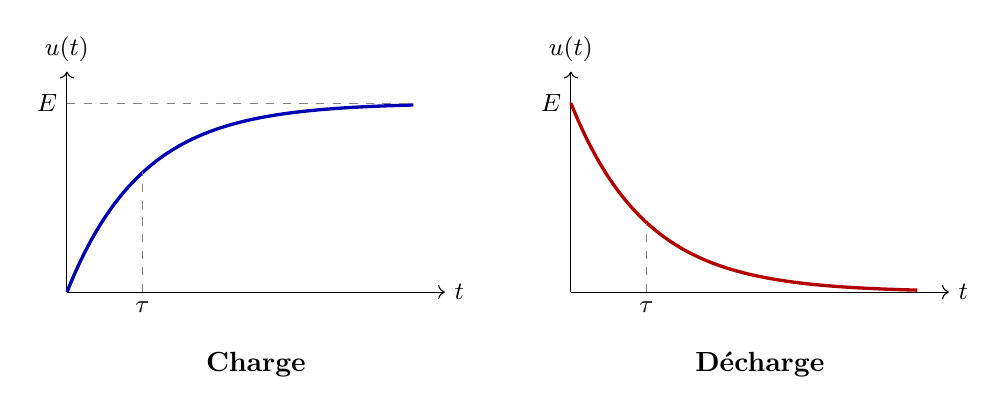
\begin{tikzpicture}[scale=0.8]
  \begin{scope}[shift={(0,0)}]
    \draw[->] (0,0) -- (6,0) node[right]{\small $t$};
    \draw[->] (0,0) -- (0,3.5) node[above]{\small $u(t)$};
    \draw[very thick, blue!70!black, domain=0:5.5, samples=100] plot(\x, {3*(1-exp(-\x/1.2))});
    \draw[dashed, gray] (0,3) -- (5.5,3);
    \node[left, font=\small] at (0,3) {$E$};
    \draw[dashed, gray] (1.2,0) -- (1.2,1.9);
    \node[below, font=\small] at (1.2,0) {$\tau$};
    \node[below] at (3,-0.8) {\textbf{Charge}};
  \end{scope}
  \begin{scope}[shift={(8,0)}]
    \draw[->] (0,0) -- (6,0) node[right]{\small $t$};
    \draw[->] (0,0) -- (0,3.5) node[above]{\small $u(t)$};
    \draw[very thick, red!70!black, domain=0:5.5, samples=100] plot(\x, {3*exp(-\x/1.2)});
    \node[left, font=\small] at (0,3) {$E$};
    \draw[dashed, gray] (1.2,0) -- (1.2,1.1);
    \node[below, font=\small] at (1.2,0) {$\tau$};
    \node[below] at (3,-0.8) {\textbf{Décharge}};
  \end{scope}
\end{tikzpicture}
\end{center}

\begin{pratique}
\textbf{Application :} $R = \SI{10}{k\ohm}$, $C = \SI{100}{\micro F}$ $\Rightarrow$ $\tau = \SI{1}{s}$. Charge complète en $\sim\SI{5}{s}$.
C'est le principe des temporisateurs, anti-rebonds, et filtres passe-bas.
\end{pratique}

\begin{intuition}
\textbf{Que fait le courant pendant la charge ?} Au tout début ($t = 0$), le condensateur est déchargé : sa tension est nulle, il se comporte comme un \textbf{court-circuit}. Tout le potentiel $E$ est aux bornes de $R$, et le courant est maximal : $i(0) = E/R$. Au fil de la charge, la tension du condensateur augmente, la tension restante aux bornes de $R$ diminue, donc le courant diminue. Quand $u \to E$, il ne reste plus rien pour ``pousser'' le courant : $i \to 0$. La charge ralentit d'elle-même --- c'est pourquoi la courbe est exponentielle, pas linéaire.
\end{intuition}

\subsection{Énergie stockée}

\begin{formule}
\[
\boxed{W = \frac{1}{2}CU^2}
\]
\end{formule}

\begin{pratique}
\textbf{Danger :} un condensateur de \SI{1000}{\micro F} / \SI{400}{V} stocke $W = 0{,}5 \times 10^{-3} \times 160000 = \SI{80}{J}$. C'est potentiellement mortel. \textbf{Toujours décharger les condensateurs avant d'intervenir sur un circuit de puissance.}
\end{pratique}

\subsection{Associations de condensateurs}

\begin{formule}
\textbf{Parallèle :} $\boxed{C_{\text{éq}} = C_1 + C_2 + \cdots}$ \qquad (les capacités s'additionnent)

\textbf{Série :} $\boxed{\dfrac{1}{C_{\text{éq}}} = \dfrac{1}{C_1} + \dfrac{1}{C_2} + \cdots}$ \qquad (les inverses s'additionnent)
\end{formule}

\begin{intuition}
C'est \textbf{l'inverse} des résistances. Parallèle = on agrandit les plaques $\Rightarrow$ plus de capacité. Série = on éloigne les plaques $\Rightarrow$ moins de capacité.
\end{intuition}

\begin{retenir}
\textbf{Les 5 idées essentielles sur le condensateur :}
\begin{enumerate}[nosep]
\item $q = Cu$ : charge proportionnelle à la tension.
\item $i = C\,\mathrm{d}u/\mathrm{d}t$ : le courant dépend de la \textit{variation} de tension.
\item Circuit ouvert en DC, laisse passer l'AC.
\item Circuit RC : $\tau = RC$, charge/décharge exponentielles.
\item Énergie : $W = \frac{1}{2}CU^2$.
\end{enumerate}
\end{retenir}

% ----------------------------------------------------------------------------
\section{Approfondissement}

\begin{approfondissement}
Construction physique, technologies, et comportement fréquentiel. Prérequis : exponentielles, équations différentielles du 1er ordre.
\end{approfondissement}

\subsection{Capacité d'un condensateur plan}

\begin{formule}
\[
\boxed{C = \varepsilon_0 \varepsilon_r \frac{S}{d}}
\]
\begin{itemize}[nosep]
\item $\varepsilon_0 = \SI{8.854e-12}{F/m}$ : permittivité du vide
\item $\varepsilon_r$ : permittivité relative du diélectrique (air $\approx 1$, FR-4 $\approx 4{,}5$, céramique haute-$\varepsilon_r$ $\sim 2000$)
\item $S$ : surface des armatures, $d$ : épaisseur du diélectrique
\end{itemize}
\end{formule}

\subsection{Technologies de condensateurs}

\begin{center}
\begin{tabular}{p{2.6cm}p{2.2cm}p{2cm}p{5.2cm}}
\toprule
\textbf{Technologie} & \textbf{Gamme} & \textbf{Tension} & \textbf{Usage typique} \\
\midrule
Céramique (MLCC) & pF--\SI{100}{\micro F} & \SI{6}{V}--\SI{1}{kV} & Découplage, HF, général \\
Film (PP, PET) & nF--\SI{10}{\micro F} & jusqu'à \SI{2}{kV} & Audio, puissance, snubber \\
Électrolytique Al & \SI{1}{\micro F}--\SI{10}{mF} & \SI{6}{V}--\SI{450}{V} & Filtrage alimentation \\
Tantale & \SI{0.1}{\micro F}--\SI{1}{mF} & \SI{2.5}{V}--\SI{50}{V} & Découplage, faible ESR \\
Supercondensateur & \SI{0.1}{F}--\SI{3000}{F} & \SI{2.5}{V}--\SI{3}{V} & Stockage d'énergie \\
\bottomrule
\end{tabular}
\end{center}

\begin{attention}
\textbf{Condensateurs polarisés :} les électrolytiques et tantales ont un sens ($+$/$-$). Les brancher à l'envers peut provoquer une \textbf{destruction explosive}. Les céramiques et films ne sont pas polarisés.
\end{attention}

\subsection{Démonstration de la charge du circuit RC}

KVL : $Ri + u = E$ avec $i = C\,\mathrm{d}u/\mathrm{d}t$ :
\[
RC\frac{\mathrm{d}u}{\mathrm{d}t} + u = E
\]

Équation différentielle du 1er ordre. Solution homogène : $u_h = Ae^{-t/RC}$. Solution particulière : $u_p = E$.

Avec $u(0) = 0$ : $u(t) = E(1 - e^{-t/RC})$. \checkmark

Courant : $i(t) = \dfrac{E}{R}e^{-t/RC}$. Le courant initial est $E/R$ (le condensateur déchargé se comporte comme un court-circuit) et décroît exponentiellement.

\subsection{Condensateur en régime sinusoïdal (aperçu)}

En régime sinusoïdal permanent, le condensateur a une \textbf{impédance} :
\[
\underline{Z}_C = \frac{1}{j\omega C} \qquad |\underline{Z}_C| = \frac{1}{\omega C}
\]

Le module \textbf{diminue} avec la fréquence : le condensateur laisse d'autant mieux passer le courant que $f$ est élevée. C'est la base du filtrage (cf.\ chapitres 13--14).

\begin{pratique}
\textbf{Exemple :} $C = \SI{100}{nF}$ : $|Z| = \SI{31.8}{k\ohm}$ à \SI{50}{Hz} (quasi ouvert), $|Z| = \SI{1.6}{\ohm}$ à \SI{1}{MHz} (quasi court-circuit). C'est pourquoi le \SI{100}{nF} est le condensateur de découplage universel.
\end{pratique}

% ----------------------------------------------------------------------------
\section{Niveau Ingénieur}

\begin{ingenieur}
Modèle réel, effets parasites, choix en conception, et lien avec le champ électrique.
\end{ingenieur}

\subsection{Modèle réel d'un condensateur}

\begin{center}
\begin{circuitikz}[scale=0.9]
  \draw (0,0) to[R, l=$\text{ESR}$] (2,0) to[L, l=$\text{ESL}$] (4,0) to[C, l=$C$] (6,0);
  \draw (0,0) -- (-0.5,0);
  \draw (6,0) -- (6.5,0);
  \draw (4.5,0) to[R, l_=$R_{\text{leak}}$, *-*] (4.5,-1.5) -| (6,0);
\end{circuitikz}
\end{center}

\begin{itemize}[nosep]
\item \textbf{ESR} : résistance série ($\SI{1}{m\ohm}$--$\SI{1}{\ohm}$). Dissipe de la puissance, limite le filtrage.
\item \textbf{ESL} : inductance série (quelques nH). Crée la fréquence de résonance série (SRF).
\item $R_{\text{leak}}$ : fuite du diélectrique ($> \SI{1}{G\ohm}$). Décharge lente sans charge externe.
\end{itemize}

\subsection{Fréquence de résonance série (SRF)}

\begin{formule}
\[
\boxed{f_{\text{SRF}} = \frac{1}{2\pi\sqrt{\text{ESL} \cdot C}}}
\]
Sous $f_{\text{SRF}}$ : capacitif. Au-dessus : \textbf{inductif} (le condensateur ne filtre plus !).
\end{formule}

\begin{pratique}
Un \SI{100}{nF} en 0805 a typiquement $f_{\text{SRF}} \sim \SI{30}{MHz}$. Au-delà, il se comporte comme une inductance. C'est pourquoi on met \textbf{plusieurs condensateurs en parallèle} de valeurs différentes (\SI{100}{nF} + \SI{1}{nF} + \SI{100}{pF}) pour couvrir une large bande. Plus le boîtier est petit, plus la SRF est élevée.
\end{pratique}

\subsection{Piège des céramiques haute capacité}

\begin{attention}
Les céramiques de classe II (X5R, X7R, Y5V) voient leur capacité \textbf{chuter fortement} avec la tension DC de polarisation. Un ``\SI{10}{\micro F} / \SI{10}{V}'' en X5R peut ne faire que \SI{3}{\micro F} à \SI{8}{V}. Toujours vérifier la courbe $C(V_{\text{DC}})$ dans la datasheet.

Les céramiques \textbf{NP0/C0G} (classe I) n'ont pas ce problème mais sont limitées à $\sim\SI{10}{nF}$.
\end{attention}

\subsection{Choix d'un condensateur selon l'application}

\begin{pratique}
\begin{itemize}[nosep]
\item \textbf{Découplage numérique :} céramique MLCC, petit boîtier, \SI{100}{nF} + \SI{1}{\micro F}.
\item \textbf{Filtrage alimentation :} électrolytique (bulk) + céramique (HF).
\item \textbf{Audio / analogique précis :} film PP ou céramique C0G/NP0.
\item \textbf{RF / micro-ondes :} céramique NP0 en 0201/0402 (SRF maximale).
\item \textbf{Puissance (snubber, EMI) :} film PP, tenue en tension et courant.
\end{itemize}
\end{pratique}

\subsection{Énergie et champ électrique}

L'énergie $W = \frac{1}{2}CU^2$ est stockée dans le \textbf{champ électrique} entre les armatures. La densité volumique d'énergie :
\[
w = \frac{1}{2}\varepsilon_0\varepsilon_r E^2 \qquad (\si{J/m^3})
\]
Pour un condensateur plan ($E = U/d$) : $W = w \cdot Sd = \frac{1}{2}\varepsilon_0\varepsilon_r\frac{S}{d}U^2 = \frac{1}{2}CU^2$. \checkmark

% === EXERCICES DU CHAPITRE 7 ===
\section*{Exercices}
\addcontentsline{toc}{section}{Exercices}

\subsection*{Niveau débutant}

\textbf{Exercice 7.1 ---} Un condensateur de \SI{47}{\micro F} est chargé sous \SI{12}{V}. Quelle charge et quelle énergie ?

\begin{pratique}
\textbf{Solution :} $q = CU = 47\times10^{-6} \times 12 = \SI{564}{\micro C}$. $W = \frac{1}{2}CU^2 = \SI{3.38}{mJ}$.
\end{pratique}

\textbf{Exercice 7.2 ---} Circuit RC : $R = \SI{4.7}{k\ohm}$, $C = \SI{10}{\micro F}$. Calculez $\tau$. Temps pour $99\%$ de charge ?

\begin{pratique}
\textbf{Solution :} $\tau = RC = \SI{47}{ms}$. $99\% = 5\tau = \SI{235}{ms}$.
\end{pratique}

\subsection*{Niveau intermédiaire}

\textbf{Exercice 7.3 ---} Un condensateur de \SI{100}{nF} chargé à \SI{5}{V} se décharge dans $R = \SI{1}{k\ohm}$. Écrivez $u(t)$, $i(t)$, $p(t)$. Vérifiez que l'énergie dissipée dans $R$ égale l'énergie initiale du condensateur.

\begin{pratique}
\textbf{Solution :} $\tau = \SI{0.1}{ms}$. $u(t) = 5e^{-t/\tau}$. $i(t) = \SI{5}{mA} \cdot e^{-t/\tau}$.

$p(t) = \SI{25}{mW} \cdot e^{-2t/\tau}$.

$W_R = \int_0^\infty p\,\mathrm{d}t = \SI{25}{mW} \times \tau/2 = \SI{1.25}{\micro J}$.

$W_C = \frac{1}{2}CU^2 = \SI{1.25}{\micro J}$. \checkmark
\end{pratique}

\textbf{Exercice 7.4 ---} Trois condensateurs : \SI{10}{\micro F}, \SI{22}{\micro F}, \SI{47}{\micro F}. $C_{\text{éq}}$ en parallèle et en série ?

\begin{pratique}
\textbf{Solution ---} Parallèle : $C_{\text{éq}} = \SI{79}{\micro F}$. Série : $1/C_{\text{éq}} = 1/10 + 1/22 + 1/47 = 0{,}167$ $\Rightarrow$ $C_{\text{éq}} \approx \SI{6}{\micro F}$.
\end{pratique}

\subsection*{Niveau ingénieur}

\textbf{Exercice 7.5 ---} Un MLCC \SI{100}{nF} / 0805 : ESR = \SI{50}{m\ohm}, ESL = \SI{1}{nH}. Calculez la SRF. Efficace à \SI{100}{MHz} ?

\begin{pratique}
\textbf{Solution :} $f_{\text{SRF}} = 1/(2\pi\sqrt{10^{-9}\times10^{-7}}) \approx \SI{16}{MHz}$.

À \SI{100}{MHz} : $|Z| \approx \omega\,\text{ESL} = 2\pi\times10^8\times10^{-9} = \SI{0.63}{\ohm}$ (inductif, ne découple plus efficacement). Ajouter un \SI{1}{nF} en 0402.
\end{pratique}

\textbf{Exercice 7.6 ---} Un céramique X5R ``\SI{10}{\micro F}'' chute à \SI{4}{\micro F} sous \SI{8}{V} DC. Filtre RC avec $R = \SI{100}{\ohm}$ conçu pour $f_c = \SI{160}{Hz}$. Quelle $f_c$ réelle ?

\begin{pratique}
\textbf{Solution :} Nominal : $f_c = 1/(2\pi\times100\times10^{-5}) = \SI{159}{Hz}$.

Réel : $f_c = 1/(2\pi\times100\times4\times10^{-6}) = \SI{398}{Hz}$. La $f_c$ a \textbf{plus que doublé} !

Solution : film PP ou céramique C0G, ou surdimensionner (prendre \SI{22}{\micro F}/\SI{25}{V}).
\end{pratique}

\subsection*{Questions de compréhension}

\begin{enumerate}[nosep]
\item Pourquoi un condensateur bloque le DC mais laisse passer l'AC ?
\item On charge un \SI{100}{\micro F} à \SI{10}{V}, on le connecte à un \SI{100}{\micro F} déchargé. Tension finale ? L'énergie est-elle conservée ?
\item Pourquoi des condensateurs de valeurs différentes en parallèle pour le découplage ?
\item Un \SI{1000}{\micro F}/\SI{400}{V} est-il dangereux après coupure de l'alimentation ?
\end{enumerate}

% === RÉSUMÉ DU CHAPITRE 7 ===
\section*{Résumé du chapitre}
\addcontentsline{toc}{section}{Résumé du chapitre}

\begin{bases}[title={\color{white} Résumé --- Les Bases}]
\begin{center}
\renewcommand{\arraystretch}{1.3}
\begin{tabular}{p{4cm}p{9cm}}
\toprule
Capacité & $q = Cu$ --- charge proportionnelle à la tension \\
Courant & $i = C\,\mathrm{d}u/\mathrm{d}t$ --- dépend de la variation de tension \\
En DC & Circuit ouvert (pas de courant) \\
Circuit RC & $\tau = RC$, charge/décharge exponentielles \\
Énergie & $W = \frac{1}{2}CU^2$ \\
Associations & Parallèle : $\sum C_k$ ; Série : $\sum 1/C_k$ \\
\bottomrule
\end{tabular}
\end{center}
\end{bases}

\begin{approfondissement}[title={\color{white} Résumé --- Approfondissement}]
\begin{center}
\renewcommand{\arraystretch}{1.3}
\begin{tabular}{p{4cm}p{9cm}}
\toprule
Condensateur plan & $C = \varepsilon_0\varepsilon_r S/d$ \\
Technologies & Céramique, film, électrolytique, tantale, supercap \\
Impédance AC & $|\underline{Z}_C| = 1/\omega C$ --- diminue avec $f$ \\
\bottomrule
\end{tabular}
\end{center}
\end{approfondissement}

\begin{ingenieur}[title={\color{white} Résumé --- Niveau Ingénieur}]
\begin{center}
\renewcommand{\arraystretch}{1.3}
\begin{tabular}{p{4cm}p{9cm}}
\toprule
Modèle réel & ESR + ESL + $R_{\text{leak}}$ \\
SRF & $1/(2\pi\sqrt{\text{ESL}\cdot C})$ --- inductif au-dessus \\
Piège X5R/X7R & $C$ chute avec $V_{\text{DC}}$ --- vérifier datasheet \\
Choix techno & Découplage, filtrage, audio, RF, puissance \\
\bottomrule
\end{tabular}
\end{center}
\end{ingenieur}


% ============================================================================
% CHAPITRE 8 : LA BOBINE (INDUCTANCE)
% ============================================================================
\chapter{La Bobine (Inductance)}

\begin{center}
\textit{La bobine stocke de l'énergie sous forme de champ magnétique.\\
C'est le dual du condensateur : elle résiste aux variations de courant,\\
comme le condensateur résiste aux variations de tension.}
\end{center}

\vspace{0.5cm}

% ----------------------------------------------------------------------------
\section{Les Bases}

\begin{bases}
La bobine (ou inductance) est le second composant qui introduit la notion de temps. Elle est le \textbf{symétrique} du condensateur à bien des égards. Prérequis : chapitres 1 à 3, et idéalement le chapitre 7 (condensateur).
\end{bases}

\subsection{Qu'est-ce qu'une bobine ?}

Une bobine est un \textbf{enroulement de fil conducteur} autour d'un support (souvent un noyau magnétique). Quand un courant la traverse, elle crée un \textbf{champ magnétique} dans et autour d'elle. Ce champ magnétique stocke de l'énergie.

\begin{analogie}
\textbf{Le volant d'inertie.} Imaginez une roue lourde (un volant) montée sur un axe :
\begin{itemize}[nosep]
\item Pour \textbf{lancer} la roue (faire passer du courant), il faut de l'effort au début : elle résiste au changement de vitesse. $\leftrightarrow$ la bobine s'oppose aux variations de courant.
\item Une fois lancée, la roue \textbf{continue de tourner} même si on arrête de pousser : elle a stocké de l'énergie cinétique. $\leftrightarrow$ la bobine maintient le courant même quand on coupe la source.
\item Pour \textbf{arrêter} la roue, il faut absorber son énergie. $\leftrightarrow$ couper brutalement le courant dans une bobine provoque une surtension (l'énergie doit aller quelque part).
\end{itemize}
\end{analogie}

\subsection{Inductance}

L'\textbf{inductance} $L$ mesure la capacité de la bobine à stocker de l'énergie magnétique pour un courant donné :

\begin{formule}
\[
\boxed{\Phi = L \cdot i}
\]
\begin{itemize}[nosep]
\item $\Phi$ : flux magnétique total embrassé par la bobine, en \textbf{webers} (Wb)
\item $L$ : inductance, en \textbf{henrys} (H)
\item $i$ : courant traversant la bobine, en ampères (A)
\end{itemize}
\vspace{0.2cm}
En pratique, on utilise des sous-multiples : $\si{mH}$, $\si{\micro H}$, $\si{nH}$.
\end{formule}

\subsection{Relation tension-courant}

La tension aux bornes d'une bobine est proportionnelle à la \textbf{vitesse de variation} du courant :

\begin{formule}
\[
\boxed{u = L \cdot \frac{\mathrm{d}i}{\mathrm{d}t}}
\]
\begin{itemize}[nosep]
\item Si le courant est constant ($\mathrm{d}i/\mathrm{d}t = 0$) : $u = 0$. La bobine se comporte comme un \textbf{court-circuit en DC} (c'est juste un fil enroulé).
\item Si le courant varie rapidement : la tension peut être très élevée.
\end{itemize}
\end{formule}

\begin{intuition}
Comparez avec le condensateur :
\begin{center}
\begin{tabular}{lcc}
\toprule
 & \textbf{Condensateur} & \textbf{Bobine} \\
\midrule
Relation & $i = C\,\mathrm{d}u/\mathrm{d}t$ & $u = L\,\mathrm{d}i/\mathrm{d}t$ \\
Stocke l'énergie dans & Champ électrique & Champ magnétique \\
S'oppose aux variations de & Tension & Courant \\
En DC & Circuit ouvert & Court-circuit \\
En HF & Court-circuit & Circuit ouvert \\
\bottomrule
\end{tabular}
\end{center}
Ce sont des composants \textbf{duaux} : chaque propriété de l'un a un miroir chez l'autre.
\end{intuition}

\begin{attention}
\textbf{Le courant dans une bobine ne peut pas varier instantanément.} Un saut de courant impliquerait une tension infinie ($u = L \times \infty$), ce qui est impossible. \textbf{Règle :} au moment d'une commutation, le courant dans la bobine garde la valeur qu'il avait juste avant.

\textbf{Mais la tension, elle, peut être énorme !} Si on tente d'interrompre brutalement le courant dans une bobine (ouverture d'un interrupteur, coupure d'un transistor), la bobine génère une \textbf{surtension} potentiellement destructrice. C'est pour cela qu'on place des \textbf{diodes de roue libre} en parallèle des bobines de relais et des moteurs : elles offrent un chemin au courant pour décroître progressivement.
\end{attention}

\subsection{Ordres de grandeur}

\begin{center}
\begin{tabular}{lll}
\toprule
\textbf{Application} & \textbf{Inductance typique} & \textbf{Ordre} \\
\midrule
Piste de PCB (parasite) & $\sim \SI{1}{nH/mm}$ & $10^{-9}$ H \\
Inductance CMS RF & \SI{1}{nH} à \SI{100}{nH} & $10^{-9}$--$10^{-7}$ H \\
Inductance de puissance (buck) & \SI{1}{\micro H} à \SI{100}{\micro H} & $10^{-6}$--$10^{-4}$ H \\
Self de filtrage secteur & \SI{1}{mH} à \SI{100}{mH} & $10^{-3}$--$10^{-1}$ H \\
Bobine de haut-parleur & $\sim \SI{1}{mH}$ & $10^{-3}$ H \\
Transformateur (primaire) & \SI{1}{H} à \SI{100}{H} & $10^{0}$--$10^{2}$ H \\
\bottomrule
\end{tabular}
\end{center}

\subsection{Charge et décharge : le circuit RL}

Le circuit RL est le dual du circuit RC.

\textbf{Établissement du courant :} on applique $E$ à un circuit $R$-$L$ série (courant initial nul) :

\begin{formule}
\[
\boxed{i(t) = \frac{E}{R}\left(1 - e^{-t/\tau}\right)} \qquad \text{avec} \quad \boxed{\tau = \frac{L}{R}}
\]
Le courant monte exponentiellement vers sa valeur finale $E/R$ (loi d'Ohm en DC).
\end{formule}

\textbf{Décroissance du courant :} la bobine parcourue par $I_0$ se décharge dans $R$ :

\begin{formule}
\[
\boxed{i(t) = I_0 \cdot e^{-t/\tau}}
\]
\end{formule}

\begin{center}
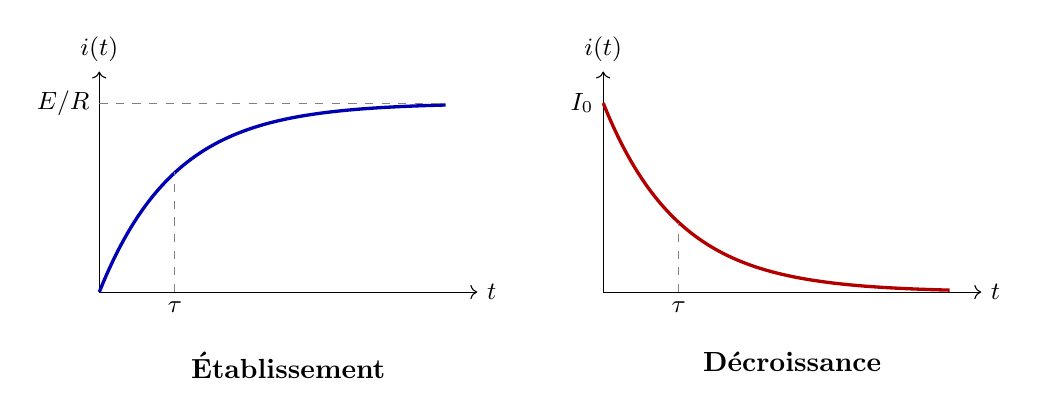
\begin{tikzpicture}[scale=0.8]
  \begin{scope}[shift={(0,0)}]
    \draw[->] (0,0) -- (6,0) node[right]{\small $t$};
    \draw[->] (0,0) -- (0,3.5) node[above]{\small $i(t)$};
    \draw[very thick, blue!70!black, domain=0:5.5, samples=100] plot(\x, {3*(1-exp(-\x/1.2))});
    \draw[dashed, gray] (0,3) -- (5.5,3);
    \node[left, font=\small] at (0,3) {$E/R$};
    \draw[dashed, gray] (1.2,0) -- (1.2,1.9);
    \node[below, font=\small] at (1.2,0) {$\tau$};
    \node[below] at (3,-0.8) {\textbf{Établissement}};
  \end{scope}
  \begin{scope}[shift={(8,0)}]
    \draw[->] (0,0) -- (6,0) node[right]{\small $t$};
    \draw[->] (0,0) -- (0,3.5) node[above]{\small $i(t)$};
    \draw[very thick, red!70!black, domain=0:5.5, samples=100] plot(\x, {3*exp(-\x/1.2)});
    \node[left, font=\small] at (0,3) {$I_0$};
    \draw[dashed, gray] (1.2,0) -- (1.2,1.1);
    \node[below, font=\small] at (1.2,0) {$\tau$};
    \node[below] at (3,-0.8) {\textbf{Décroissance}};
  \end{scope}
\end{tikzpicture}
\end{center}

\begin{intuition}
\textbf{Que fait la tension pendant l'établissement ?} Au début ($t = 0$), le courant est nul : la bobine se comporte comme un circuit ouvert. Toute la tension $E$ est aux bornes de $L$ et rien aux bornes de $R$. Le courant commence à croître. Au fil du temps, le courant augmente, la tension aux bornes de $R$ ($= Ri$) augmente, donc celle aux bornes de $L$ ($= E - Ri$) diminue, et la croissance du courant ralentit. À $t \to \infty$ : $i = E/R$, $u_L = 0$. La bobine est devenue un simple fil.
\end{intuition}

\begin{pratique}
Comparaison des constantes de temps :
\begin{center}
\begin{tabular}{lcc}
\toprule
 & \textbf{RC} & \textbf{RL} \\
\midrule
$\tau$ & $RC$ & $L/R$ \\
$\tau$ augmente si & $R$ ou $C$ augmente & $L$ augmente ou $R$ diminue \\
Grandeur qui ne saute pas & Tension ($u_C$) & Courant ($i_L$) \\
\bottomrule
\end{tabular}
\end{center}
\end{pratique}

\subsection{Énergie stockée}

\begin{formule}
\[
\boxed{W = \frac{1}{2}LI^2}
\]
$W$ en joules, $L$ en henrys, $I$ en ampères.
\end{formule}

\begin{attention}
L'énergie stockée dans une bobine peut être dangereuse. Si on ouvre brutalement un circuit portant \SI{10}{A} à travers une inductance de \SI{10}{mH}, l'énergie $W = 0{,}5 \times 0{,}01 \times 100 = \SI{0.5}{J}$ doit être dissipée. Sans chemin de décharge (diode de roue libre), la tension monte jusqu'à claquer un composant ou créer un arc électrique.
\end{attention}

\subsection{Associations d'inductances}

\begin{formule}
\textbf{Série :} $\boxed{L_{\text{éq}} = L_1 + L_2 + \cdots}$ \qquad (comme les résistances en série)

\textbf{Parallèle :} $\boxed{\dfrac{1}{L_{\text{éq}}} = \dfrac{1}{L_1} + \dfrac{1}{L_2} + \cdots}$ \qquad (comme les résistances en parallèle)
\end{formule}

\begin{intuition}
Les inductances s'associent \textbf{comme les résistances} (et à l'inverse des condensateurs). Série = plus de tours de fil = plus d'inductance. Parallèle = les flux se partagent = moins d'inductance.
\end{intuition}

\begin{retenir}
\textbf{Les 5 idées essentielles sur la bobine :}
\begin{enumerate}[nosep]
\item $u = L\,\mathrm{d}i/\mathrm{d}t$ : la tension dépend de la \textit{variation} du courant.
\item Court-circuit en DC, circuit ouvert en HF.
\item Le courant dans une bobine ne peut pas sauter $\Rightarrow$ surtension si coupure brutale.
\item Circuit RL : $\tau = L/R$, établissement/décroissance exponentiels.
\item Énergie : $W = \frac{1}{2}LI^2$.
\end{enumerate}
\end{retenir}

% ----------------------------------------------------------------------------
\section{Approfondissement}

\begin{approfondissement}
Construction physique, technologies, saturation du noyau. Prérequis : exponentielles, équations différentielles du 1er ordre.
\end{approfondissement}

\subsection{Inductance d'un solénoïde}

Un solénoïde (bobine longue) de $N$ spires, section $S$, longueur $\ell$, avec un noyau de perméabilité relative $\mu_r$ :

\begin{formule}
\[
\boxed{L = \mu_0 \mu_r \frac{N^2 S}{\ell}}
\]
\begin{itemize}[nosep]
\item $\mu_0 = 4\pi\times10^{-7}$ H/m : perméabilité du vide
\item $\mu_r$ : perméabilité relative du noyau (air : 1, ferrite : 100--10\,000, fer doux : $\sim 5000$)
\item $N$ : nombre de spires (l'inductance croît comme $N^2$ !)
\item $S$ : section du noyau (m$^2$), $\ell$ : longueur du solénoïde (m)
\end{itemize}
\end{formule}

\begin{pratique}
\textbf{Exemple :} 100 spires sur un noyau de ferrite ($\mu_r = 2000$), section \SI{1}{cm^2}, longueur \SI{5}{cm} :

$L = 4\pi\times10^{-7} \times 2000 \times \frac{100^2 \times 10^{-4}}{0{,}05} = \SI{50}{mH}$.

Sans noyau ($\mu_r = 1$) : $L = \SI{25}{\micro H}$. Le noyau multiplie l'inductance par $\mu_r = 2000$.
\end{pratique}

\subsection{Technologies d'inductances}

\begin{center}
\begin{tabular}{p{2.5cm}p{2.5cm}p{2cm}p{5cm}}
\toprule
\textbf{Type} & \textbf{Gamme} & \textbf{Courant} & \textbf{Usage} \\
\midrule
Air (sans noyau) & nH--\SI{10}{\micro H} & Faible & RF, VHF, UHF (pas de pertes noyau) \\
Ferrite (NiZn, MnZn) & \SI{1}{\micro H}--\SI{100}{mH} & Moyen & Filtrage, découplage, SMPS \\
Fer poudre & \SI{1}{\micro H}--\SI{10}{mH} & Fort & Puissance, convertisseurs DC-DC \\
Noyau laminé (fer-silicium) & mH--H & Très fort & Transformateurs, selfs secteur \\
CMS (bobinée ou multicouche) & nH--\SI{100}{\micro H} & Variable & Général, PCB, filtrage \\
\bottomrule
\end{tabular}
\end{center}

\subsection{Saturation du noyau magnétique}

\begin{attention}
\textbf{Phénomène critique :} quand le courant dépasse une certaine valeur ($I_{\text{sat}}$), le noyau magnétique \textbf{sature} : sa perméabilité $\mu_r$ chute brutalement. L'inductance s'effondre, le composant ne stocke plus d'énergie efficacement, et le courant peut augmenter de manière incontrôlée (surtout dans un convertisseur de puissance).

\textbf{Règle de conception :} toujours vérifier que le courant crête (DC + ondulation) reste \textbf{en dessous} de $I_{\text{sat}}$ indiqué dans la datasheet. Les ferrites saturent typiquement à $B_{\text{sat}} \approx \SI{300}{mT}$ à \SI{500}{mT}, le fer poudre à $\sim\SI{1}{T}$.
\end{attention}

\subsection{Démonstration du circuit RL}

KVL : $u_R + u_L = E$ avec $u_R = Ri$ et $u_L = L\,\mathrm{d}i/\mathrm{d}t$ :
\[
L\frac{\mathrm{d}i}{\mathrm{d}t} + Ri = E
\]

Même type d'équation que le RC. Avec $i(0) = 0$ :

$i(t) = \dfrac{E}{R}(1 - e^{-Rt/L})$. Constante de temps : $\tau = L/R$. \checkmark

La tension aux bornes de la bobine : $u_L(t) = E\,e^{-t/\tau}$.

\subsection{Bobine en régime sinusoïdal (aperçu)}

En régime sinusoïdal, la bobine a une \textbf{impédance} :
\[
\underline{Z}_L = j\omega L \qquad |\underline{Z}_L| = \omega L
\]

Le module \textbf{augmente} avec la fréquence : la bobine laisse passer le DC mais bloque les signaux HF. C'est le comportement \textbf{inverse} du condensateur.

\begin{pratique}
\textbf{Exemple :} $L = \SI{10}{\micro H}$ : $|Z| = \SI{3.1}{m\ohm}$ à \SI{50}{Hz} (quasi court-circuit), $|Z| = \SI{63}{\ohm}$ à \SI{1}{MHz} (bloque). C'est le principe des \textbf{selfs de filtrage} (ferrite beads, chokes) qui laissent passer le DC d'alimentation mais bloquent le bruit HF.
\end{pratique}

% ----------------------------------------------------------------------------
\section{Niveau Ingénieur}

\begin{ingenieur}
Modèle réel, pertes dans le noyau, inductance mutuelle, et considérations de conception.
\end{ingenieur}

\subsection{Modèle réel d'une inductance}

\begin{center}
\begin{circuitikz}[scale=0.9]
  \draw (0,0) to[R, l=$R_{\text{DC}}$] (2.5,0) to[L, l=$L$] (5,0) to[short] (6,0);
  \draw (3,0) to[C, l_=$C_p$, *-*] (3,-1.5) -| (5.5,0);
  \draw (0,0) -- (-0.5,0);
  \draw (6,0) -- (6.5,0);
\end{circuitikz}
\end{center}

\begin{itemize}[nosep]
\item $R_{\text{DC}}$ (\textit{DC Resistance}) : résistance du fil de cuivre. $\SI{1}{m\ohm}$ à quelques $\Omega$ selon la taille. Dissipe de la puissance ($P = R_{\text{DC}} I^2$) et limite le rendement.
\item $C_p$ : capacité parasite inter-spires. Crée une \textbf{fréquence de résonance parallèle} (SRF) au-delà de laquelle l'inductance se comporte comme un \textit{condensateur}.
\item Pertes noyau (non modélisées par un composant simple) : voir ci-dessous.
\end{itemize}

\subsection{SRF et comportement fréquentiel}

\begin{formule}
\[
\boxed{f_{\text{SRF}} = \frac{1}{2\pi\sqrt{L \cdot C_p}}}
\]
En dessous de $f_{\text{SRF}}$ : inductif ($|Z|$ augmente avec $f$).

Au-dessus : \textbf{capacitif} ($|Z|$ diminue avec $f$) --- l'inductance ne fonctionne plus !
\end{formule}

\begin{pratique}
C'est le \textbf{miroir} du condensateur : le condensateur devient inductif au-dessus de sa SRF, et l'inductance devient capacitive au-dessus de la sienne. En conception, on vérifie \textit{toujours} que la fréquence de travail est bien en dessous de la SRF du composant.

Ordres de grandeur : inductance CMS \SI{10}{\micro H} $\rightarrow$ SRF $\sim \SI{5}{MHz}$ à \SI{50}{MHz} selon le boîtier et la techno.
\end{pratique}

\subsection{Pertes dans le noyau}

Les noyaux magnétiques dissipent de l'énergie par deux mécanismes :

\textbf{1. Pertes par hystérésis :} le cycle B-H du matériau magnétique n'est pas réversible. À chaque cycle de magnétisation, une énergie proportionnelle à l'\textit{aire du cycle d'hystérésis} est dissipée en chaleur. Ces pertes augmentent avec la fréquence et l'amplitude de l'excitation.

\textbf{2. Pertes par courants de Foucault :} le champ magnétique variable induit des courants dans le noyau lui-même (qui est conducteur). Ces courants dissipent de la puissance par effet Joule. On les réduit en utilisant des noyaux \textit{laminés} (tôles isolées empilées) ou des matériaux à haute résistivité (ferrites).

\begin{formule}
Modèle empirique de Steinmetz (très utilisé en puissance) :
\[
\boxed{P_{\text{core}} = k \cdot f^\alpha \cdot B_{\text{max}}^\beta \cdot V_{\text{core}}}
\]
avec $k$, $\alpha \approx 1{,}5$--$2$ et $\beta \approx 2$--$3$ dépendant du matériau. $V_{\text{core}}$ : volume du noyau.
\end{formule}

\subsection{Inductance mutuelle et couplage (aperçu)}

Quand deux bobines sont proches, le flux magnétique de l'une traverse l'autre. On définit l'\textbf{inductance mutuelle} $M$ :
\[
u_2 = M \frac{\mathrm{d}i_1}{\mathrm{d}t}
\]

Le \textbf{coefficient de couplage} $k = M/\sqrt{L_1 L_2}$ varie de 0 (pas de couplage) à 1 (couplage parfait).

\begin{pratique}
\textbf{Applications :}
\begin{itemize}[nosep]
\item \textbf{Transformateur :} $k \approx 0{,}95$--$0{,}999$ (noyau fermé, couplage quasi parfait).
\item \textbf{Inductances couplées SMPS :} $k \approx 0{,}5$--$0{,}9$ (flyback, SEPIC).
\item \textbf{Diaphonie entre pistes PCB :} $k \ll 1$ (couplage parasite non souhaité).
\item \textbf{Charge sans fil (Qi) :} $k \approx 0{,}3$--$0{,}7$.
\end{itemize}
Le transformateur sera traité en détail dans un chapitre dédié.
\end{pratique}

\subsection{Énergie et champ magnétique}

L'énergie $W = \frac{1}{2}LI^2$ est stockée dans le \textbf{champ magnétique} à l'intérieur (et autour) de la bobine. La densité volumique d'énergie :
\[
w = \frac{1}{2}\frac{B^2}{\mu_0 \mu_r} = \frac{1}{2}\mu_0\mu_r H^2 \qquad (\si{J/m^3})
\]

\begin{attention}
Paradoxe apparent : un matériau à fort $\mu_r$ (ferrite) stocke \textit{moins} d'énergie par unité de volume qu'un entrefer à $\mu_r = 1$ (pour un même $B$). C'est pourquoi les inductances de puissance ont un \textbf{entrefer} (gap) : c'est dans l'air de l'entrefer que l'essentiel de l'énergie est stocké, pas dans la ferrite. La ferrite sert à ``canaliser'' le flux magnétique, pas à stocker l'énergie.
\end{attention}

% === EXERCICES DU CHAPITRE 8 ===
\section*{Exercices}
\addcontentsline{toc}{section}{Exercices}

\subsection*{Niveau débutant}

\textbf{Exercice 8.1 ---} Une bobine de \SI{100}{mH} est parcourue par un courant de \SI{2}{A}. Quelle énergie stocke-t-elle ? Si le courant est coupé en \SI{1}{ms}, quelle tension moyenne apparaît à ses bornes ?

\begin{pratique}
\textbf{Solution :} $W = \frac{1}{2}LI^2 = 0{,}5 \times 0{,}1 \times 4 = \SI{0.2}{J}$.

Tension moyenne : $|u| = L\,|\Delta i / \Delta t| = 0{,}1 \times 2/0{,}001 = \SI{200}{V}$ ! C'est la surtension de coupure.
\end{pratique}

\textbf{Exercice 8.2 ---} Un circuit RL a $R = \SI{100}{\ohm}$ et $L = \SI{50}{mH}$. Calculez $\tau$. Au bout de $5\tau$, quel est le courant si $E = \SI{10}{V}$ ?

\begin{pratique}
\textbf{Solution :} $\tau = L/R = 0{,}05/100 = \SI{0.5}{ms}$.

À $5\tau$ : $i = (E/R)(1 - e^{-5}) = (10/100)(1 - 0{,}0067) \approx \SI{99.3}{mA} \approx E/R$.
\end{pratique}

\subsection*{Niveau intermédiaire}

\textbf{Exercice 8.3 ---} On veut fabriquer une inductance de \SI{1}{mH} avec un noyau de ferrite ($\mu_r = 2000$), section \SI{0.5}{cm^2}, longueur \SI{3}{cm}. Combien de spires faut-il ?

\begin{pratique}
\textbf{Solution :} $L = \mu_0\mu_r N^2 S/\ell \Rightarrow N = \sqrt{L\ell/(\mu_0\mu_r S)}$

$N = \sqrt{10^{-3} \times 0{,}03 / (4\pi\times10^{-7} \times 2000 \times 0{,}5\times10^{-4})}$

$= \sqrt{3\times10^{-5} / (1{,}257\times10^{-7})} = \sqrt{239} \approx 15{,}5$ spires. On prend $N = 16$.

Vérification : $L = 4\pi\times10^{-7} \times 2000 \times 256 \times 0{,}5\times10^{-4} / 0{,}03 = \SI{1.07}{mH}$. \checkmark
\end{pratique}

\textbf{Exercice 8.4 ---} Une bobine de relais ($L = \SI{50}{mH}$, $R_{\text{bobine}} = \SI{100}{\ohm}$) est alimentée par \SI{12}{V}. Calculez le courant en régime permanent, $\tau$, et la surtension si on coupe le courant sans diode de roue libre (temps de coupure $\sim\SI{1}{\micro s}$).

\begin{pratique}
\textbf{Solution :} $I = E/R = 12/100 = \SI{120}{mA}$. $\tau = L/R = \SI{0.5}{ms}$.

Surtension : $|u| \approx L\,|di/dt| = 0{,}05 \times 0{,}12/10^{-6} = \SI{6000}{V}$ !

C'est suffisant pour détruire un transistor MOSFET (\SI{30}{V} max typique). La diode de roue libre est \textbf{indispensable}.
\end{pratique}

\subsection*{Niveau ingénieur}

\textbf{Exercice 8.5 ---} Une inductance de puissance de \SI{10}{\micro H} avec un noyau de ferrite ($B_{\text{sat}} = \SI{400}{mT}$, section $S = \SI{0.5}{cm^2}$, $N = 20$ spires) est utilisée dans un convertisseur buck. Calculez le courant de saturation. Si le convertisseur fonctionne à \SI{500}{kHz} avec un courant moyen de \SI{3}{A} et une ondulation crête-à-crête de \SI{2}{A}, le noyau sature-t-il ?

\begin{pratique}
\textbf{Solution :} $B = LI/(NS) \Rightarrow I_{\text{sat}} = B_{\text{sat}} \cdot N \cdot S / L$

$I_{\text{sat}} = 0{,}4 \times 20 \times 0{,}5\times10^{-4} / 10^{-5} = 0{,}4 \times 10^{-3} / 10^{-5} = \SI{40}{A}$.

Courant crête : $I_{\text{pk}} = I_{\text{moy}} + \Delta I/2 = 3 + 1 = \SI{4}{A}$.

$I_{\text{pk}} = \SI{4}{A} \ll I_{\text{sat}} = \SI{40}{A}$. Pas de saturation, marge confortable.
\end{pratique}

\textbf{Exercice 8.6 ---} Deux bobines identiques ($L = \SI{1}{mH}$) sont couplées avec $k = 0{,}8$. Calculez $M$. Si elles sont montées en série ``aiding'' (flux dans le même sens), quelle est l'inductance totale ? Et en ``opposing'' ?

\begin{pratique}
\textbf{Solution :} $M = k\sqrt{L_1 L_2} = 0{,}8 \times \SI{1}{mH} = \SI{0.8}{mH}$.

Aiding : $L_{\text{tot}} = L_1 + L_2 + 2M = 1 + 1 + 1{,}6 = \SI{3.6}{mH}$.

Opposing : $L_{\text{tot}} = L_1 + L_2 - 2M = 1 + 1 - 1{,}6 = \SI{0.4}{mH}$.

Le couplage peut \textbf{augmenter ou diminuer} l'inductance totale selon le sens relatif des enroulements.
\end{pratique}

\subsection*{Questions de compréhension}

\begin{enumerate}[nosep]
\item Pourquoi une bobine se comporte-t-elle comme un court-circuit en DC mais comme un circuit ouvert en haute fréquence ? Comparez avec le condensateur.
\item On ouvre brutalement un interrupteur dans un circuit inductif. Que se passe-t-il ? Pourquoi un arc électrique peut-il se former ?
\item Pourquoi les inductances de puissance (convertisseurs DC-DC) ont-elles un entrefer dans leur noyau de ferrite ?
\item Une piste de PCB de \SI{1}{cm} a une inductance d'environ \SI{10}{nH}. Si un circuit numérique commute \SI{1}{A} en \SI{1}{ns}, quelle tension parasite cette piste induit-elle ? Est-ce problématique ?
\end{enumerate}

% === RÉSUMÉ DU CHAPITRE 8 ===
\section*{Résumé du chapitre}
\addcontentsline{toc}{section}{Résumé du chapitre}

\begin{bases}[title={\color{white} Résumé --- Les Bases}]
\begin{center}
\renewcommand{\arraystretch}{1.3}
\begin{tabular}{p{4cm}p{9cm}}
\toprule
Tension & $u = L\,\mathrm{d}i/\mathrm{d}t$ --- dépend de la variation de courant \\
En DC & Court-circuit (juste un fil) \\
Surtension & Couper $i$ brutalement $\Rightarrow$ $u$ énorme $\Rightarrow$ diode de roue libre \\
Circuit RL & $\tau = L/R$, établissement/décroissance exponentiels \\
Énergie & $W = \frac{1}{2}LI^2$ --- dans le champ magnétique \\
Associations & Série : $\sum L_k$ ; Parallèle : $\sum 1/L_k$ (comme les résistances) \\
\bottomrule
\end{tabular}
\end{center}
\end{bases}

\begin{approfondissement}[title={\color{white} Résumé --- Approfondissement}]
\begin{center}
\renewcommand{\arraystretch}{1.3}
\begin{tabular}{p{4cm}p{9cm}}
\toprule
Solénoïde & $L = \mu_0\mu_r N^2 S/\ell$ \\
Saturation & $B > B_{\text{sat}} \Rightarrow \mu_r$ chute $\Rightarrow L$ s'effondre \\
Impédance AC & $|\underline{Z}_L| = \omega L$ --- augmente avec $f$ \\
\bottomrule
\end{tabular}
\end{center}
\end{approfondissement}

\begin{ingenieur}[title={\color{white} Résumé --- Niveau Ingénieur}]
\begin{center}
\renewcommand{\arraystretch}{1.3}
\begin{tabular}{p{4cm}p{9cm}}
\toprule
Modèle réel & $R_{\text{DC}} + C_p$ parasite $\Rightarrow$ SRF (capacitif au-dessus) \\
Pertes noyau & Hystérésis + Foucault --- Steinmetz : $P \propto f^\alpha B^\beta$ \\
Couplage & $M = k\sqrt{L_1L_2}$, $k \in [0,1]$ --- base du transformateur \\
Entrefer & Stocke l'énergie (pas la ferrite !) --- critique en puissance \\
\bottomrule
\end{tabular}
\end{center}
\end{ingenieur}


% ============================================================================
% CHAPITRE 9 : CIRCUITS RC, RL, RLC
% ============================================================================
\chapter{Circuits RC, RL et RLC}

\begin{center}
\textit{Les combinaisons de R, L et C sont la base de tous les filtres,\\
oscillateurs et circuits de temporisation de l'électronique.}
\end{center}

\vspace{0.5cm}

Les chapitres 7 et 8 ont étudié le condensateur et la bobine séparément. Ce chapitre les \textbf{combine} pour révéler des comportements nouveaux : oscillations, résonance, amortissement. Ce sont les briques fondamentales de toute l'électronique analogique.

% ----------------------------------------------------------------------------
\section{Les Bases}

\begin{bases}
Cette section présente les comportements qualitatifs des circuits RC, RL et RLC. Prérequis : chapitres 7 et 8.
\end{bases}

\subsection{Rappel : les trois comportements fondamentaux}

\begin{center}
\begin{tabular}{lccc}
\toprule
\textbf{Composant} & \textbf{En DC} & \textbf{En HF} & \textbf{Stocke l'énergie dans} \\
\midrule
Résistance $R$ & $R$ & $R$ & Rien (dissipe) \\
Condensateur $C$ & Circuit ouvert & Court-circuit & Champ électrique \\
Bobine $L$ & Court-circuit & Circuit ouvert & Champ magnétique \\
\bottomrule
\end{tabular}
\end{center}

\begin{intuition}
La résistance \textit{dissipe} l'énergie (irréversiblement en chaleur). Le condensateur et la bobine \textit{stockent} l'énergie (réversiblement). Quand on les combine, l'énergie peut \textbf{osciller} entre les deux formes de stockage (électrique $\leftrightarrow$ magnétique), pendant que la résistance l'amortit progressivement.
\end{intuition}

\subsection{Le circuit RC (rappel synthétique)}

On l'a vu au chapitre 7. L'essentiel :

\begin{formule}
\textbf{Constante de temps :} $\tau = RC$.

\textbf{Charge :} $u_C(t) = E(1 - e^{-t/\tau})$.

\textbf{Décharge :} $u_C(t) = E\,e^{-t/\tau}$.

\textbf{Comportement fréquentiel :} le circuit RC série forme un \textbf{filtre passe-bas} (sortie prise aux bornes de $C$) ou un \textbf{filtre passe-haut} (sortie prise aux bornes de $R$). La fréquence de coupure est :
\[
\boxed{f_c = \frac{1}{2\pi RC}}
\]
\end{formule}

\subsection{Le circuit RL (rappel synthétique)}

Vu au chapitre 8. L'essentiel :

\begin{formule}
\textbf{Constante de temps :} $\tau = L/R$.

\textbf{Établissement :} $i(t) = (E/R)(1 - e^{-t/\tau})$.

\textbf{Décroissance :} $i(t) = I_0\,e^{-t/\tau}$.

\textbf{Comportement fréquentiel :} le RL série forme un \textbf{filtre passe-haut} (sortie aux bornes de $L$) ou \textbf{passe-bas} (sortie aux bornes de $R$). Fréquence de coupure :
\[
\boxed{f_c = \frac{R}{2\pi L}}
\]
\end{formule}

\subsection{Le circuit RLC série : un comportement nouveau}

Quand on associe $R$, $L$ et $C$ en série, un phénomène nouveau apparaît : l'énergie peut \textbf{osciller} entre $L$ et $C$.

\begin{analogie}
\textbf{La balançoire.} Une balançoire (ou un pendule) oscille entre énergie potentielle (en haut) et énergie cinétique (en bas). Le frottement de l'air l'amortit progressivement.

Dans le circuit RLC :
\begin{itemize}[nosep]
\item L'énergie du condensateur ($\frac{1}{2}Cu^2$) $\leftrightarrow$ énergie potentielle.
\item L'énergie de la bobine ($\frac{1}{2}Li^2$) $\leftrightarrow$ énergie cinétique.
\item La résistance $R$ $\leftrightarrow$ le frottement (amortissement).
\end{itemize}
\end{analogie}

La réponse à un échelon de tension dépend de la valeur de $R$ par rapport à $L$ et $C$. On distingue trois régimes :

\begin{center}
\begin{tabular}{lll}
\toprule
\textbf{Régime} & \textbf{Condition} & \textbf{Comportement} \\
\midrule
Sur-amorti & $R > 2\sqrt{L/C}$ & Pas d'oscillation, retour lent \\
Critique & $R = 2\sqrt{L/C}$ & Retour le plus rapide sans oscillation \\
Sous-amorti & $R < 2\sqrt{L/C}$ & Oscillations amorties \\
\bottomrule
\end{tabular}
\end{center}

\begin{center}
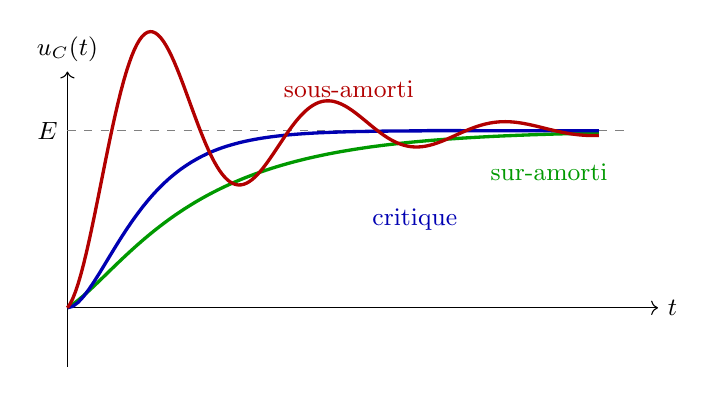
\begin{tikzpicture}[scale=0.75]
  \draw[->] (0,0) -- (10,0) node[right]{\small $t$};
  \draw[->] (0,-1) -- (0,4) node[above]{\small $u_C(t)$};
  \draw[dashed, gray] (0,3) -- (9.5,3);
  \node[left, font=\small] at (0,3) {$E$};
  
  % Sur-amorti
  \draw[very thick, green!60!black, domain=0:9, samples=100] plot(\x, {3*(1-1.2*exp(-0.5*\x)+0.2*exp(-2*\x))});
  \node[green!60!black, font=\small, right] at (7,2.3) {sur-amorti};
  
  % Critique
  \draw[very thick, blue!70!black, domain=0:9, samples=100] plot(\x, {3*(1-(1+1.5*\x)*exp(-1.5*\x))});
  \node[blue!70!black, font=\small, right] at (5,1.5) {critique};
  
  % Sous-amorti
  \draw[very thick, red!70!black, domain=0:9, samples=200] plot(\x, {3*(1-exp(-0.4*\x)*cos(120*\x))});
  \node[red!70!black, font=\small, right] at (3.5,3.7) {sous-amorti};
\end{tikzpicture}
\end{center}

\begin{attention}
\textbf{Le régime critique} ($R = 2\sqrt{L/C}$) est le cas idéal en instrumentation et en asservissement : c'est le régime qui atteint la valeur finale \textbf{le plus vite possible sans dépasser} ($0\%$ d'overshoot). En pratique, on vise souvent un léger sous-amortissement pour un bon compromis rapidité/dépassement.
\end{attention}

\subsection{Fréquence propre du circuit LC}

Sans résistance ($R = 0$), le circuit LC oscille indéfiniment à sa \textbf{fréquence propre} :

\begin{formule}
\[
\boxed{f_0 = \frac{1}{2\pi\sqrt{LC}}} \qquad \text{ou} \qquad \boxed{\omega_0 = \frac{1}{\sqrt{LC}}}
\]
C'est la fréquence à laquelle l'énergie fait un aller-retour complet entre $C$ et $L$.
\end{formule}

\begin{pratique}
\textbf{Exemple :} $L = \SI{1}{mH}$, $C = \SI{100}{nF}$ :

$f_0 = 1/(2\pi\sqrt{10^{-3}\times10^{-7}}) = 1/(2\pi\times\SI{e-5}{}) \approx \SI{15.9}{kHz}$.

C'est une fréquence audio. Avec $L = \SI{10}{nH}$ et $C = \SI{1}{pF}$ : $f_0 \approx \SI{1.6}{GHz}$ (domaine RF).
\end{pratique}

\begin{retenir}
\textbf{L'essentiel sur les circuits RC, RL, RLC :}
\begin{enumerate}[nosep]
\item RC et RL : comportement du 1er ordre (exponentielle, constante de temps $\tau$).
\item RLC : comportement du 2nd ordre (oscillations possibles, 3 régimes).
\item Fréquence propre LC : $f_0 = 1/(2\pi\sqrt{LC})$.
\item $R$ contrôle l'amortissement : plus $R$ est grand (RLC série), plus l'amortissement est fort.
\end{enumerate}
\end{retenir}

% ----------------------------------------------------------------------------
\section{Approfondissement}

\begin{approfondissement}
Équations différentielles, facteur de qualité, réponses temporelles et fréquentielles. Prérequis : équations différentielles du 2nd ordre, exponentielles complexes.
\end{approfondissement}

\subsection{Équation différentielle du circuit RLC série}

KVL : $u_R + u_L + u_C = E$, soit $Ri + L\,\mathrm{d}i/\mathrm{d}t + u_C = E$ avec $i = C\,\mathrm{d}u_C/\mathrm{d}t$ :

\begin{formule}
\[
\boxed{LC\frac{\mathrm{d}^2 u_C}{\mathrm{d}t^2} + RC\frac{\mathrm{d}u_C}{\mathrm{d}t} + u_C = E}
\]
Forme canonique (en divisant par $LC$) :
\[
\frac{\mathrm{d}^2 u_C}{\mathrm{d}t^2} + \frac{\omega_0}{Q}\frac{\mathrm{d}u_C}{\mathrm{d}t} + \omega_0^2\, u_C = \omega_0^2\, E
\]
avec $\omega_0 = 1/\sqrt{LC}$ et $Q = \frac{1}{R}\sqrt{L/C}$ (facteur de qualité).
\end{formule}

\subsection{Facteur de qualité $Q$}

Le \textbf{facteur de qualité} $Q$ caractérise l'amortissement du circuit :

\begin{formule}
\[
\boxed{Q = \frac{1}{R}\sqrt{\frac{L}{C}}} \qquad \text{(RLC série)}
\]
\begin{itemize}[nosep]
\item $Q < 0{,}5$ : sur-amorti (pas d'oscillation)
\item $Q = 0{,}5$ : critique (amortissement optimal)
\item $Q > 0{,}5$ : sous-amorti (oscillations)
\end{itemize}
Plus $Q$ est grand, moins il y a d'amortissement. $Q = \infty$ ($R = 0$) : oscillations permanentes.
\end{formule}

\begin{intuition}
$Q$ mesure le rapport entre l'énergie stockée et l'énergie dissipée par cycle. Un $Q$ élevé signifie que le circuit ``résonne'' longtemps avant de s'amortir, comme une cloche de qualité ($Q \sim 1000$) comparée à un bloc de bois ($Q \sim 1$).

\textbf{Physiquement :} $Q = 2\pi \times \dfrac{\text{énergie stockée}}{\text{énergie dissipée par cycle}}$.
\end{intuition}

\subsection{Solutions de l'équation différentielle}

L'équation caractéristique $s^2 + (\omega_0/Q)s + \omega_0^2 = 0$ a pour discriminant :

$\Delta = \omega_0^2(1/Q^2 - 4)$

\textbf{Trois cas :}

\textbf{1. Sur-amorti ($Q < 0{,}5$, $\Delta > 0$) :} deux racines réelles négatives $s_1, s_2$.
\[
u_C(t) = E + A_1 e^{s_1 t} + A_2 e^{s_2 t}
\]
Retour monotone vers $E$, sans oscillation.

\textbf{2. Critique ($Q = 0{,}5$, $\Delta = 0$) :} racine double $s = -\omega_0$.
\[
u_C(t) = E + (A + Bt)e^{-\omega_0 t}
\]
Retour le plus rapide sans dépassement.

\textbf{3. Sous-amorti ($Q > 0{,}5$, $\Delta < 0$) :} racines complexes conjuguées $s = -\alpha \pm j\omega_d$.
\[
u_C(t) = E + A\,e^{-\alpha t}\cos(\omega_d t + \varphi)
\]
avec $\alpha = \omega_0/(2Q)$ (amortissement) et $\omega_d = \omega_0\sqrt{1 - 1/(4Q^2)}$ (pseudo-pulsation).

\begin{pratique}
\textbf{Dépassement (overshoot) :} en régime sous-amorti, la tension dépasse la valeur finale avant de s'y stabiliser. Le premier dépassement vaut approximativement :
\[
D(\%) \approx 100 \times e^{-\pi/\sqrt{4Q^2 - 1}}
\]
Pour $Q = 1$ : $D \approx 16\%$. Pour $Q = 5$ : $D \approx 73\%$. Pour $Q = 0{,}7$ (souvent visé) : $D \approx 5\%$.
\end{pratique}

\subsection{Circuit RLC parallèle}

Le RLC parallèle est le \textbf{dual} du RLC série. Les trois composants sont branchés entre les deux mêmes n\oe uds.

\begin{formule}
Pour le RLC parallèle, le facteur de qualité est :
\[
\boxed{Q = R\sqrt{\frac{C}{L}}} \qquad \text{(RLC parallèle --- inverse du série !)}
\]
La fréquence propre reste $\omega_0 = 1/\sqrt{LC}$.
\end{formule}

\begin{attention}
\textbf{Piège classique :} dans le RLC série, $Q$ augmente quand $R$ diminue. Dans le RLC parallèle, c'est l'inverse : $Q$ augmente quand $R$ augmente. C'est la conséquence de la dualité série/parallèle.
\end{attention}

\subsection{Résonance (aperçu --- développé au Ch.\ 12)}

Quand on excite un circuit RLC par une source sinusoïdale à la fréquence $f_0$, l'impédance du circuit atteint un \textbf{extremum} :
\begin{itemize}[nosep]
\item \textbf{RLC série :} l'impédance est \textit{minimale} à $f_0$ (elle vaut $R$). Le courant est maximal. C'est la \textbf{résonance série}.
\item \textbf{RLC parallèle :} l'impédance est \textit{maximale} à $f_0$ (elle vaut $R$). Le courant est minimal. C'est la \textbf{résonance parallèle} (ou antirésonance).
\end{itemize}

La \textbf{bande passante} à $-3\,\text{dB}$ est liée au facteur de qualité :
\begin{formule}
\[
\boxed{\Delta f = \frac{f_0}{Q}}
\]
Plus $Q$ est élevé, plus la résonance est ``pointue'' (sélective). C'est le principe des filtres, des oscillateurs et des récepteurs radio.
\end{formule}

% ----------------------------------------------------------------------------
\section{Niveau Ingénieur}

\begin{ingenieur}
Stabilité, pôles et zéros, amortissement en conception, et liens avec les systèmes asservis.
\end{ingenieur}

\subsection{Pôles et zéros dans le plan complexe}

L'équation caractéristique $s^2 + (\omega_0/Q)s + \omega_0^2 = 0$ donne deux \textbf{pôles} dans le plan complexe. Leur position détermine tout le comportement transitoire :

\begin{itemize}[nosep]
\item \textbf{Pôles réels négatifs} ($Q < 0{,}5$) : sur-amorti. Les pôles sont sur l'axe réel négatif.
\item \textbf{Pôle double réel} ($Q = 0{,}5$) : critique. Un seul pôle (double) sur l'axe réel.
\item \textbf{Pôles complexes conjugués} ($Q > 0{,}5$) : sous-amorti. Les pôles sont dans le demi-plan gauche, symétriques par rapport à l'axe réel. Leur partie imaginaire donne la pseudo-pulsation $\omega_d$, leur partie réelle donne le taux d'amortissement $\alpha$.
\item \textbf{Pôles imaginaires purs} ($R = 0$, $Q = \infty$) : oscillations permanentes (non amorties). En pratique, cela n'existe pas (il y a toujours des pertes).
\end{itemize}

\begin{attention}
Si un pôle a une partie réelle positive, le système est \textbf{instable} : la réponse diverge exponentiellement. Cela ne se produit pas avec des composants passifs (R, L, C), mais peut arriver avec des composants actifs (amplificateurs avec rétroaction positive). C'est le fondement de l'analyse de stabilité en automatique et en conception d'amplificateurs.
\end{attention}

\subsection{Le facteur de qualité en conception réelle}

\begin{pratique}
\textbf{Valeurs typiques de $Q$ selon l'application :}
\begin{center}
\begin{tabular}{ll}
\toprule
\textbf{Application} & \textbf{$Q$ typique} \\
\midrule
Filtre anti-aliasing (ADC) & $0{,}5$--$0{,}7$ (Butterworth, Bessel) \\
Filtre audio (égaliseur) & $1$--$10$ \\
Circuit résonant radio (AM) & $50$--$200$ \\
Filtre à quartz & $10\,000$--$100\,000$ \\
Cavité micro-ondes & $1000$--$50\,000$ \\
Résonateur MEMS & $> 100\,000$ \\
\bottomrule
\end{tabular}
\end{center}
En conception, $Q$ est limité par les pertes (ESR du condensateur, résistance du fil, pertes du noyau). On ne peut pas obtenir un $Q$ arbitrairement élevé avec des composants passifs seuls --- c'est pourquoi on utilise des \textbf{filtres actifs} (avec AOP) pour synthétiser des $Q$ élevés à basse fréquence.
\end{pratique}

\subsection{Lien avec les systèmes asservis}

Le circuit RLC du 2nd ordre est \textit{mathématiquement identique} à un système mécanique masse-ressort-amortisseur, à un asservissement de position, ou à un PLL. La fonction de transfert canonique du 2nd ordre :

\begin{formule}
\[
\boxed{H(s) = \frac{\omega_0^2}{s^2 + \frac{\omega_0}{Q}s + \omega_0^2}} \qquad \text{(passe-bas du 2nd ordre)}
\]
\end{formule}

Les paramètres $\omega_0$ et $Q$ (ou de manière équivalente le coefficient d'amortissement $\zeta = 1/(2Q)$) caractérisent \textit{tous} les systèmes du 2nd ordre, qu'ils soient électriques, mécaniques ou logiciels. Maîtriser le RLC, c'est maîtriser la moitié de l'automatique.

\subsection{Composants parasites et circuits RLC non voulus}

\begin{attention}
En conception réelle, les circuits RLC apparaissent \textbf{sans qu'on le veuille} :
\begin{itemize}[nosep]
\item Un condensateur réel (ESL + C) forme un circuit LC série avec une fréquence de résonance (SRF). Vu au chapitre 7.
\item Une inductance réelle ($L$ + $C_p$) forme un circuit LC parallèle. Vu au chapitre 8.
\item Une piste de PCB a une inductance ($\sim\SI{1}{nH/mm}$) et une capacité ($\sim\SI{0.5}{pF/cm}$) parasites. Sur une piste de \SI{10}{cm} : $L \approx \SI{10}{nH}$, $C \approx \SI{0.5}{pF}$, $f_0 \approx \SI{2.3}{GHz}$.
\item Un câble coaxial est une ligne de transmission distribuée, modélisée par une cascade infinie de cellules RLC.
\end{itemize}
Ces résonances parasites sont une source majeure de problèmes en CEM, en intégrité du signal et en stabilité des alimentations. Le travail de l'ingénieur consiste souvent à \textbf{amortir} ces résonances (ajout de résistances, choix de composants à faible $Q$, placement stratégique des découplages).
\end{attention}

% === EXERCICES DU CHAPITRE 9 ===
\section*{Exercices}
\addcontentsline{toc}{section}{Exercices}

\subsection*{Niveau débutant}

\textbf{Exercice 9.1 ---} Un circuit RC a $R = \SI{1}{k\ohm}$ et $C = \SI{10}{nF}$. Calculez $\tau$ et $f_c$.

\begin{pratique}
\textbf{Solution :} $\tau = RC = 10^3 \times 10^{-8} = \SI{10}{\micro s}$. $f_c = 1/(2\pi\tau) = 1/(2\pi\times10^{-5}) \approx \SI{15.9}{kHz}$.
\end{pratique}

\textbf{Exercice 9.2 ---} Un circuit LC a $L = \SI{100}{\micro H}$ et $C = \SI{100}{pF}$. Quelle est sa fréquence propre ? Dans quel domaine de fréquence se situe-t-on ?

\begin{pratique}
\textbf{Solution :} $f_0 = 1/(2\pi\sqrt{10^{-4}\times10^{-10}}) = 1/(2\pi\times\SI{e-7}{}) \approx \SI{1.59}{MHz}$. Domaine des \textbf{ondes courtes} (HF radio).
\end{pratique}

\subsection*{Niveau intermédiaire}

\textbf{Exercice 9.3 ---} Un circuit RLC série a $R = \SI{100}{\ohm}$, $L = \SI{10}{mH}$, $C = \SI{1}{\micro F}$. Calculez $f_0$, $Q$ et déterminez le régime (sur-amorti, critique, sous-amorti). Quel est le premier dépassement ?

\begin{pratique}
\textbf{Solution :} $\omega_0 = 1/\sqrt{LC} = 1/\sqrt{10^{-2}\times10^{-6}} = 1/\sqrt{10^{-8}} = \SI{e4}{rad/s}$.

$f_0 = \omega_0/(2\pi) \approx \SI{1.59}{kHz}$.

$Q = (1/R)\sqrt{L/C} = (1/100)\sqrt{10^{-2}/10^{-6}} = (1/100)\times100 = 1$.

$Q = 1 > 0{,}5$ : régime \textbf{sous-amorti}.

Dépassement : $D \approx 100\,e^{-\pi/\sqrt{4\times1-1}} = 100\,e^{-\pi/\sqrt{3}} \approx 100\times0{,}163 \approx 16\%$.
\end{pratique}

\textbf{Exercice 9.4 ---} Même circuit, mais avec $R = \SI{200}{\ohm}$. Le régime change-t-il ? Quelle valeur de $R$ donne le régime critique ?

\begin{pratique}
\textbf{Solution :} $Q = (1/200)\times100 = 0{,}5$. C'est exactement le \textbf{régime critique}.

Pour $R = \SI{200}{\ohm}$ : $Q = 0{,}5$, critique.

Pour $R > \SI{200}{\ohm}$ : $Q < 0{,}5$, sur-amorti.

Valeur critique : $R_c = 2\sqrt{L/C} = 2\times100 = \SI{200}{\ohm}$. \checkmark
\end{pratique}

\subsection*{Niveau ingénieur}

\textbf{Exercice 9.5 ---} Un filtre passe-bande est réalisé avec un RLC série ($f_0 = \SI{1}{MHz}$, $Q = 50$). Calculez la bande passante. Si $C = \SI{100}{pF}$, quelles sont les valeurs de $L$ et $R$ ?

\begin{pratique}
\textbf{Solution :} $\Delta f = f_0/Q = 10^6/50 = \SI{20}{kHz}$.

$L = 1/(\omega_0^2 C) = 1/((2\pi\times10^6)^2 \times 10^{-10}) = 1/(3{,}95\times10^{13}\times10^{-10}) = \SI{253}{\micro H}$.

$R = (1/Q)\sqrt{L/C} = (1/50)\sqrt{253\times10^{-6}/10^{-10}} = (1/50)\times\SI{1592}{} = \SI{31.8}{\ohm}$.

Ce filtre sélectionne une bande de \SI{20}{kHz} autour de \SI{1}{MHz} --- typique d'un récepteur radio AM.
\end{pratique}

\textbf{Exercice 9.6 ---} Un bus d'alimentation sur PCB a une inductance parasite de \SI{5}{nH} et un condensateur de découplage de \SI{10}{\micro F} (ESR = \SI{10}{m\ohm}). Calculez la fréquence de résonance et le $Q$. Cette résonance est-elle problématique ? Comment l'amortir ?

\begin{pratique}
\textbf{Solution :} $f_0 = 1/(2\pi\sqrt{5\times10^{-9}\times10^{-5}}) = 1/(2\pi\times\SI{7.07e-8}{}) \approx \SI{712}{kHz}$.

$Q = (1/\text{ESR})\sqrt{L/C} = (1/0{,}01)\sqrt{5\times10^{-9}/10^{-5}} = 100\times\SI{7.07e-4}{} \approx 0{,}07$.

$Q = 0{,}07 \ll 0{,}5$ : \textbf{très sur-amorti}, pas de problème de résonance. L'ESR du condensateur amortit suffisamment.

Si on avait un condensateur céramique (ESR $\sim\SI{1}{m\ohm}$) : $Q \approx 0{,}7$, sous-amorti ! On verrait des oscillations sur le bus d'alimentation. Solution : ajouter une petite résistance en série (``ESR snubber'') ou un condensateur électrolytique en parallèle (fort ESR naturel) pour amortir.
\end{pratique}

\subsection*{Questions de compréhension}

\begin{enumerate}[nosep]
\item Pourquoi un circuit LC pur (sans résistance) oscille-t-il indéfiniment en théorie ? En pratique, s'arrête-t-il ? Pourquoi ?
\item On veut qu'un capteur atteigne sa valeur finale le plus vite possible sans dépasser. Quel régime faut-il choisir et pourquoi ?
\item Expliquez pourquoi les fabricants de condensateurs spécifient l'ESR : est-ce toujours un défaut ? Donnez un exemple où un ESR élevé est souhaitable.
\item Un oscillateur à quartz a un $Q$ de 50\,000. Comparez avec un circuit LC classique ($Q \sim 100$). Quelles conséquences pratiques ?
\end{enumerate}

% === RÉSUMÉ DU CHAPITRE 9 ===
\section*{Résumé du chapitre}
\addcontentsline{toc}{section}{Résumé du chapitre}

\begin{bases}[title={\color{white} Résumé --- Les Bases}]
\begin{center}
\renewcommand{\arraystretch}{1.3}
\begin{tabular}{p{4cm}p{9cm}}
\toprule
RC & $\tau = RC$, filtre passe-bas/haut, $f_c = 1/(2\pi RC)$ \\
RL & $\tau = L/R$, filtre passe-bas/haut, $f_c = R/(2\pi L)$ \\
RLC & 2nd ordre : 3 régimes (sur-amorti, critique, sous-amorti) \\
Fréquence propre & $f_0 = 1/(2\pi\sqrt{LC})$ \\
\bottomrule
\end{tabular}
\end{center}
\end{bases}

\begin{approfondissement}[title={\color{white} Résumé --- Approfondissement}]
\begin{center}
\renewcommand{\arraystretch}{1.3}
\begin{tabular}{p{4cm}p{9cm}}
\toprule
Facteur de qualité & $Q = (1/R)\sqrt{L/C}$ (série), $Q = R\sqrt{C/L}$ (parallèle) \\
Amortissement & $Q < 0{,}5$ : sur-amorti, $Q = 0{,}5$ : critique, $Q > 0{,}5$ : sous-amorti \\
Bande passante & $\Delta f = f_0/Q$ \\
Résonance & Série : $|Z|$ min $= R$ ; Parallèle : $|Z|$ max $= R$ \\
\bottomrule
\end{tabular}
\end{center}
\end{approfondissement}

\begin{ingenieur}[title={\color{white} Résumé --- Niveau Ingénieur}]
\begin{center}
\renewcommand{\arraystretch}{1.3}
\begin{tabular}{p{4cm}p{9cm}}
\toprule
Pôles & Position dans le plan $s$ détermine le transitoire \\
$H(s)$ canonique & $\omega_0^2/(s^2 + \omega_0 s/Q + \omega_0^2)$ --- universel (élec, méca, auto) \\
$Q$ en conception & Limité par pertes composants, filtres actifs pour $Q$ élevé \\
RLC parasites & Pistes, condensateurs, inductances résonent --- amortir ! \\
\bottomrule
\end{tabular}
\end{center}
\end{ingenieur}


% ============================================================================
% PARTIE III : RÉGIME SINUSOÏDAL
% ============================================================================
\part{Régime Sinusoïdal}

% ============================================================================
% CHAPITRE 10 : NOTATION COMPLEXE ET IMPÉDANCES
% ============================================================================
\chapter{Notation Complexe et Impédances}

\begin{center}
\textit{Les nombres complexes transforment les équations différentielles\\
des circuits en simples équations algébriques.\\
C'est l'outil le plus puissant de l'électronicien.}
\end{center}

\vspace{0.5cm}

Jusqu'ici, nous avons analysé les circuits en continu (DC) ou en transitoire (exponentielles, RC, RL). Mais la majorité des signaux réels sont \textbf{périodiques} : secteur 50\,Hz, audio, radio, horloge numérique\ldots{} Ce chapitre introduit l'outil mathématique qui permet d'analyser ces signaux sans résoudre d'équation différentielle : la \textbf{notation complexe}.

% ----------------------------------------------------------------------------
\section{Les Bases}

\begin{bases}
Cette section est un \textbf{rappel mathématique complet} sur les nombres complexes, suivi de leur application aux circuits. On part de zéro : aucune connaissance préalable sur les complexes n'est nécessaire.
\end{bases}

\subsection{Pourquoi les nombres complexes ?}

En régime sinusoïdal, les tensions et courants sont de la forme :
\[
u(t) = \hat{U}\cos(\omega t + \varphi)
\]

Analyser un circuit avec de tels signaux revient à résoudre des équations différentielles à chaque fois. C'est long et pénible.

\begin{intuition}
Les nombres complexes sont un \textbf{raccourci de calcul}, pas une abstraction inutile. Ils permettent de remplacer :
\begin{itemize}[nosep]
\item les dérivées par des multiplications ($\mathrm{d}/\mathrm{d}t \to j\omega$),
\item les intégrales par des divisions ($\int\mathrm{d}t \to 1/(j\omega)$),
\item les équations différentielles par de simples lois d'Ohm généralisées ($\underline{U} = \underline{Z}\cdot\underline{I}$).
\end{itemize}
Le résultat final est \textit{toujours} un nombre réel (une tension ou un courant physique). Les complexes ne sont qu'un outil de passage.
\end{intuition}

\subsection{Rappel mathématique : les nombres complexes}

\subsubsection*{Définition}

Un \textbf{nombre complexe} $z$ s'écrit :
\[
z = a + jb
\]
\begin{itemize}[nosep]
\item $a = \text{Re}(z)$ : \textbf{partie réelle}
\item $b = \text{Im}(z)$ : \textbf{partie imaginaire}
\item $j$ : l'\textbf{unité imaginaire}, définie par $j^2 = -1$
\end{itemize}

\begin{attention}
En mathématiques, on note $i$ l'unité imaginaire. En électronique, on utilise $j$ pour éviter la confusion avec le courant $i$. C'est une convention universelle en ingénierie.
\end{attention}

\subsubsection*{Représentation dans le plan complexe}

Chaque nombre complexe $z = a + jb$ correspond à un \textbf{point} (ou un \textbf{vecteur}) dans le plan :
\begin{itemize}[nosep]
\item L'axe horizontal = axe réel ($a$)
\item L'axe vertical = axe imaginaire ($b$)
\end{itemize}

\begin{center}
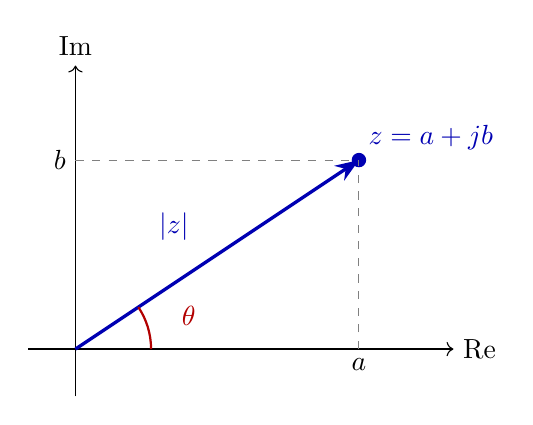
\begin{tikzpicture}[scale=1.2]
  \draw[->] (-0.5,0) -- (4,0) node[right]{Re};
  \draw[->] (0,-0.5) -- (0,3) node[above]{Im};
  
  % Point z
  \draw[very thick, blue!70!black, -{Stealth[length=3mm]}] (0,0) -- (3,2);
  \filldraw[blue!70!black] (3,2) circle (2pt);
  \node[above right, blue!70!black] at (3,2) {$z = a + jb$};
  
  % Projections
  \draw[dashed, gray] (3,0) -- (3,2);
  \draw[dashed, gray] (0,2) -- (3,2);
  \node[below] at (3,0) {$a$};
  \node[left] at (0,2) {$b$};
  
  % Module et argument
  \draw[red!70!black, thick] (0.8,0) arc[start angle=0, end angle=33.7, radius=0.8];
  \node[red!70!black] at (1.2,0.35) {$\theta$};
  \node[blue!70!black, left] at (1.3,1.3) {$|z|$};
\end{tikzpicture}
\end{center}

\subsubsection*{Module et argument}

Tout nombre complexe peut aussi s'écrire en coordonnées \textbf{polaires} :
\begin{itemize}[nosep]
\item \textbf{Module} : $|z| = \sqrt{a^2 + b^2}$ (distance à l'origine = ``longueur'' du vecteur)
\item \textbf{Argument} : $\theta = \arctan(b/a)$ (angle avec l'axe réel)
\end{itemize}

\subsubsection*{Les trois formes d'écriture}

\begin{formule}
\[
\boxed{z = a + jb = |z|\,e^{j\theta} = |z|(\cos\theta + j\sin\theta)}
\]
\begin{itemize}[nosep]
\item \textbf{Forme algébrique} : $a + jb$ --- pratique pour additionner/soustraire.
\item \textbf{Forme exponentielle} : $|z|\,e^{j\theta}$ --- pratique pour multiplier/diviser.
\item \textbf{Forme trigonométrique} : $|z|(\cos\theta + j\sin\theta)$ --- fait le lien entre les deux.
\end{itemize}
\end{formule}

La relation $e^{j\theta} = \cos\theta + j\sin\theta$ est la \textbf{formule d'Euler}. C'est la clé de voûte de toute la notation complexe en électronique.

\subsubsection*{Opérations sur les complexes}

\begin{center}
\renewcommand{\arraystretch}{1.5}
\begin{tabular}{lll}
\toprule
\textbf{Opération} & \textbf{Forme algébrique} & \textbf{Forme exponentielle} \\
\midrule
Addition & $(a_1+a_2) + j(b_1+b_2)$ & (pas pratique) \\
Multiplication & (développer) & $|z_1||z_2|\,e^{j(\theta_1+\theta_2)}$ \\
Division & (conjugué) & $\dfrac{|z_1|}{|z_2|}\,e^{j(\theta_1-\theta_2)}$ \\
Conjugué & $z^* = a - jb$ & $|z|\,e^{-j\theta}$ \\
\bottomrule
\end{tabular}
\end{center}

\begin{intuition}
\textbf{Multiplier par $e^{j\theta}$, c'est tourner de $\theta$ dans le plan complexe.} C'est ce qui fait la puissance de cette notation : un déphasage (décalage temporel) devient une simple rotation.

Cas particuliers essentiels :
\begin{itemize}[nosep]
\item $\times\, j = \times\, e^{j\pi/2}$ : rotation de $+90°$.
\item $\times\, (-j) = \times\, e^{-j\pi/2}$ : rotation de $-90°$.
\item $\times\, (-1) = \times\, e^{j\pi}$ : rotation de $180°$ (inversion de signe).
\end{itemize}
\end{intuition}

\subsection{Application aux circuits : la notation complexe}

En régime sinusoïdal permanent de pulsation $\omega$, toute grandeur du circuit peut s'écrire :
\[
u(t) = \hat{U}\cos(\omega t + \varphi_u) = \text{Re}\left[\hat{U}\,e^{j(\omega t + \varphi_u)}\right] = \text{Re}\left[\underline{U}\,e^{j\omega t}\right]
\]

On définit l'\textbf{amplitude complexe} (ou \textbf{phaseur}) :

\begin{formule}
\[
\boxed{\underline{U} = \hat{U}\,e^{j\varphi_u}}
\]
$\underline{U}$ contient \textit{toute} l'information sur le signal sinusoïdal : son amplitude $\hat{U}$ (module) et sa phase $\varphi_u$ (argument). Le facteur $e^{j\omega t}$, commun à tous les signaux du circuit, est omis.
\end{formule}

\begin{attention}
\textbf{Condition fondamentale :} la notation complexe n'est valable qu'en \textbf{régime sinusoïdal permanent} (une seule fréquence $\omega$). Elle ne s'applique pas directement aux transitoires ni aux signaux non sinusoïdaux (pour ceux-ci, on utilise la transformée de Fourier ou de Laplace).
\end{attention}

\subsection{L'impédance : la loi d'Ohm généralisée}

L'\textbf{impédance} $\underline{Z}$ d'un dipôle est le rapport de la tension complexe au courant complexe :

\begin{formule}
\[
\boxed{\underline{U} = \underline{Z} \cdot \underline{I}}
\]
C'est la \textbf{loi d'Ohm généralisée}. Elle a exactement la même forme que $U = RI$, mais avec des grandeurs complexes. Toutes les méthodes des chapitres 3 à 6 (diviseur, Thévenin, Kirchhoff, superposition\ldots) restent valables en remplaçant $R$ par $\underline{Z}$.
\end{formule}

\subsection{Impédance des trois composants de base}

\begin{formule}
\textbf{Résistance :}
\[
\boxed{\underline{Z}_R = R}
\]
L'impédance est réelle : tension et courant sont en phase.

\vspace{0.3cm}
\textbf{Condensateur :}
\[
\boxed{\underline{Z}_C = \frac{1}{j\omega C} = \frac{-j}{\omega C}}
\]
L'impédance est \textbf{imaginaire négative} : le courant est en avance de $90°$ sur la tension. Le module $|\underline{Z}_C| = 1/(\omega C)$ \textbf{diminue} avec $\omega$ : le condensateur laisse de mieux en mieux passer quand la fréquence augmente.

\vspace{0.3cm}
\textbf{Inductance :}
\[
\boxed{\underline{Z}_L = j\omega L}
\]
L'impédance est \textbf{imaginaire positive} : le courant est en retard de $90°$ sur la tension. Le module $|\underline{Z}_L| = \omega L$ \textbf{augmente} avec $\omega$ : la bobine bloque de plus en plus quand la fréquence augmente.
\end{formule}

\begin{intuition}
\textbf{D'où viennent ces formules ?} Pour le condensateur : $i = C\,\mathrm{d}u/\mathrm{d}t$. En notation complexe, $\mathrm{d}/\mathrm{d}t \to j\omega$, donc $\underline{I} = j\omega C\,\underline{U}$, soit $\underline{Z}_C = \underline{U}/\underline{I} = 1/(j\omega C)$.

Pour la bobine : $u = L\,\mathrm{d}i/\mathrm{d}t \to \underline{U} = j\omega L\,\underline{I}$, soit $\underline{Z}_L = j\omega L$.

La dérivée temporelle est devenue une simple multiplication par $j\omega$. C'est \textit{toute} la puissance de la méthode.
\end{intuition}

\subsection{Comportement en basse et haute fréquence}

Comprendre le comportement asymptotique des composants est \textbf{fondamental} pour l'analyse rapide des circuits :

\begin{formule}
\begin{center}
\renewcommand{\arraystretch}{1.8}
\begin{tabular}{lcccc}
\toprule
\textbf{Composant} & $\underline{Z}$ & \textbf{BF} ($\omega \to 0$) & \textbf{HF} ($\omega \to \infty$) & \textbf{Comportement} \\
\midrule
$R$ & $R$ & $R$ & $R$ & Constant \\
$C$ & $\dfrac{1}{j\omega C}$ & $|\underline{Z}| \to \infty$ (ouvert) & $|\underline{Z}| \to 0$ (court-circuit) & Passe-haut \\[6pt]
$L$ & $j\omega L$ & $|\underline{Z}| \to 0$ (court-circuit) & $|\underline{Z}| \to \infty$ (ouvert) & Passe-bas \\
\bottomrule
\end{tabular}
\end{center}
\end{formule}

\begin{intuition}
\textbf{Comment analyser intuitivement un circuit en BF et HF :}
\begin{enumerate}[nosep]
\item \textbf{En BF} ($\omega \to 0$, ``quasi-DC'') : remplacer chaque condensateur par un \textbf{circuit ouvert} et chaque bobine par un \textbf{court-circuit} (fil). Analyser le circuit simplifié.
\item \textbf{En HF} ($\omega \to \infty$) : remplacer chaque condensateur par un \textbf{court-circuit} et chaque bobine par un \textbf{circuit ouvert}. Analyser le circuit simplifié.
\item Le comportement réel à la fréquence de travail est ``entre les deux''.
\end{enumerate}
Cette méthode d'analyse asymptotique est la première chose à faire face à n'importe quel circuit analogique. Elle donne immédiatement le type de filtre, le gain DC, le gain HF, et les fréquences de transition.
\end{intuition}

\begin{pratique}
\textbf{Exemple --- filtre RC passe-bas :} $R$ en série, $C$ en parallèle (sortie aux bornes de $C$).
\begin{itemize}[nosep]
\item \textbf{BF :} $C$ = ouvert $\Rightarrow$ tout le signal passe $\Rightarrow$ $V_{\text{out}} = V_{\text{in}}$. Gain = 1.
\item \textbf{HF :} $C$ = court-circuit $\Rightarrow$ la sortie est court-circuitée à la masse $\Rightarrow$ $V_{\text{out}} = 0$. Gain = 0.
\end{itemize}
Conclusion immédiate : c'est un \textbf{passe-bas} (laisse passer le BF, bloque le HF). La fréquence de transition est $f_c = 1/(2\pi RC)$.
\end{pratique}

\begin{retenir}
\textbf{Les 5 idées essentielles de ce chapitre :}
\begin{enumerate}[nosep]
\item Les complexes transforment les dérivées en multiplications ($\mathrm{d}/\mathrm{d}t \to j\omega$).
\item L'impédance généralise la résistance : $\underline{U} = \underline{Z}\cdot\underline{I}$.
\item $\underline{Z}_R = R$, \quad $\underline{Z}_C = 1/(j\omega C)$, \quad $\underline{Z}_L = j\omega L$.
\item En BF : $C$ = ouvert, $L$ = fil. En HF : $C$ = fil, $L$ = ouvert.
\item Toutes les méthodes (Kirchhoff, Thévenin, diviseur\ldots) restent valables avec $\underline{Z}$.
\end{enumerate}
\end{retenir}

% ----------------------------------------------------------------------------
\section{Approfondissement}

\begin{approfondissement}
Admittance, associations d'impédances, diviseurs complexes, déphasage. Prérequis : section précédente (complexes de base).
\end{approfondissement}

\subsection{Admittance}

L'\textbf{admittance} $\underline{Y}$ est l'inverse de l'impédance :

\begin{formule}
\[
\boxed{\underline{Y} = \frac{1}{\underline{Z}} = G + jB}
\]
\begin{itemize}[nosep]
\item $G$ : conductance (partie réelle), en siemens (S)
\item $B$ : susceptance (partie imaginaire), en siemens (S)
\end{itemize}
Pour un condensateur : $\underline{Y}_C = j\omega C$. Pour une bobine : $\underline{Y}_L = 1/(j\omega L)$.
\end{formule}

L'admittance est particulièrement utile pour les associations en \textbf{parallèle} (les admittances s'additionnent, comme les conductances).

\subsection{Associations d'impédances}

Les règles sont identiques à celles des résistances :

\begin{formule}
\textbf{Série :} $\boxed{\underline{Z}_{\text{éq}} = \underline{Z}_1 + \underline{Z}_2 + \cdots}$

\textbf{Parallèle :} $\boxed{\dfrac{1}{\underline{Z}_{\text{éq}}} = \dfrac{1}{\underline{Z}_1} + \dfrac{1}{\underline{Z}_2} + \cdots}$

Cas de 2 en parallèle : $\underline{Z}_{\text{éq}} = \dfrac{\underline{Z}_1 \cdot \underline{Z}_2}{\underline{Z}_1 + \underline{Z}_2}$
\end{formule}

\subsection{Diviseur de tension en complexe}

Le diviseur de tension se généralise naturellement :
\begin{formule}
\[
\boxed{\underline{V}_{\text{out}} = \underline{V}_{\text{in}} \cdot \frac{\underline{Z}_2}{\underline{Z}_1 + \underline{Z}_2}}
\]
C'est exactement la même formule qu'en DC, avec $R$ remplacé par $\underline{Z}$. Le résultat est un nombre complexe dont le module donne le \textbf{gain} et l'argument donne le \textbf{déphasage}.
\end{formule}

\textbf{Exemple --- Filtre RC passe-bas :} $\underline{Z}_1 = R$, $\underline{Z}_2 = 1/(j\omega C)$.

\[
\underline{H}(\omega) = \frac{\underline{V}_{\text{out}}}{\underline{V}_{\text{in}}} = \frac{1/(j\omega C)}{R + 1/(j\omega C)} = \frac{1}{1 + j\omega RC} = \frac{1}{1 + j\omega/\omega_c}
\]

avec $\omega_c = 1/(RC)$.

\begin{itemize}[nosep]
\item \textbf{Module} (gain) : $|H| = \dfrac{1}{\sqrt{1 + (\omega/\omega_c)^2}}$
\item \textbf{Argument} (déphasage) : $\varphi = -\arctan(\omega/\omega_c)$
\end{itemize}

À $\omega = \omega_c$ : $|H| = 1/\sqrt{2} \approx 0{,}707$ ($-3$ dB) et $\varphi = -45°$.

\subsection{Déphasage : signification physique}

\begin{intuition}
Le \textbf{déphasage} $\varphi$ entre tension et courant indique le décalage temporel entre les deux signaux :
\[
\Delta t = \frac{\varphi}{\omega} = \frac{\varphi}{2\pi f}
\]
\begin{itemize}[nosep]
\item $\varphi = 0$ : $u$ et $i$ en phase (résistance pure).
\item $\varphi = +90°$ : $i$ en retard sur $u$ (inductance : le courant ``réagit lentement'').
\item $\varphi = -90°$ : $i$ en avance sur $u$ (condensateur : le courant ``anticipe'' la variation de tension).
\end{itemize}
\end{intuition}

\subsection{Impédance d'un circuit RLC série à la résonance}

À la fréquence de résonance $\omega_0 = 1/\sqrt{LC}$ :
\[
\underline{Z}_L + \underline{Z}_C = j\omega_0 L + \frac{1}{j\omega_0 C} = j\omega_0 L - j\frac{1}{\omega_0 C}
\]

Or $\omega_0^2 LC = 1$, donc $\omega_0 L = 1/(\omega_0 C)$. Les deux termes se compensent exactement :
\[
\underline{Z}_{\text{RLC}}(\omega_0) = R
\]

\begin{intuition}
\textbf{À la résonance}, l'inductance et le condensateur s'annulent mutuellement. Le circuit se comporte comme une \textbf{simple résistance}. C'est pour cela que le courant est maximal (en série) ou minimal (en parallèle) à la résonance.
\end{intuition}

\subsection{Théorème de Millman en complexe}

La formule de Millman se généralise immédiatement :
\begin{formule}
\[
\boxed{\underline{V}_A = \frac{\displaystyle\sum_k \frac{\underline{E}_k}{\underline{Z}_k} + \sum_j \underline{I}_{s,j}}{\displaystyle\sum_k \frac{1}{\underline{Z}_k}}}
\]
Chaque $\underline{Z}_k$ peut contenir des R, L, C. Toutes les méthodes du chapitre 6 s'étendent naturellement au domaine fréquentiel.
\end{formule}

% ----------------------------------------------------------------------------
\section{Niveau Ingénieur}

\begin{ingenieur}
Fonction de transfert, diagramme de Bode (aperçu), impédance de sortie en fréquence, et transition vers les paramètres S.
\end{ingenieur}

\subsection{Fonction de transfert}

La \textbf{fonction de transfert} $\underline{H}(\omega)$ (ou $H(j\omega)$) d'un circuit est le rapport entrée/sortie en notation complexe :

\begin{formule}
\[
\boxed{\underline{H}(\omega) = \frac{\underline{V}_{\text{out}}}{\underline{V}_{\text{in}}} = |H(\omega)|\,e^{j\varphi(\omega)}}
\]
\begin{itemize}[nosep]
\item $|H(\omega)|$ : \textbf{gain} en fonction de la fréquence
\item $\varphi(\omega)$ : \textbf{phase} en fonction de la fréquence
\end{itemize}
Ce concept sera développé en détail au chapitre 13 (fonctions de transfert et Bode).
\end{formule}

\subsection{Le décibel (dB)}

Le gain est souvent exprimé en \textbf{décibels} :

\begin{formule}
\[
\boxed{G_{\text{dB}} = 20\log_{10}|H|}
\]
\begin{itemize}[nosep]
\item $|H| = 1$ $\Rightarrow$ $G = \SI{0}{dB}$ (pas d'amplification ni d'atténuation)
\item $|H| = 1/\sqrt{2} \approx 0{,}707$ $\Rightarrow$ $G = \SI{-3}{dB}$ (fréquence de coupure)
\item $|H| = 0{,}1$ $\Rightarrow$ $G = \SI{-20}{dB}$ (atténuation d'un facteur 10)
\item $|H| = 10$ $\Rightarrow$ $G = \SI{+20}{dB}$ (amplification d'un facteur 10)
\end{itemize}
\end{formule}

\begin{pratique}
\textbf{Règles rapides pour le dB :}
\begin{itemize}[nosep]
\item $\times 2$ en tension $= +6$ dB. $\times 10 = +20$ dB. $\times 100 = +40$ dB.
\item $\div 2 = -6$ dB. $\div 10 = -20$ dB.
\item Un filtre du 1er ordre atténue de $-20$ dB/décade au-delà de $f_c$.
\item Un filtre du 2nd ordre : $-40$ dB/décade.
\end{itemize}
\end{pratique}

\subsection{Impédance de Thévenin en fréquence}

L'impédance de sortie d'un circuit n'est pas constante --- elle \textbf{varie avec la fréquence}. On écrit :
\[
\underline{Z}_{\text{out}}(\omega) = \underline{Z}_{\text{th}}(\omega)
\]

\begin{pratique}
\textbf{Exemple critique --- alimentation avec câble inductif :}

Une alimentation parfaite ($Z_{\text{out}} \approx 0$ en DC) est connectée à un circuit via un câble de \SI{10}{cm} ($L \approx \SI{50}{nH}$). Le condensateur de découplage en bout de câble est un \SI{10}{\micro F} (ESR $= \SI{5}{m\ohm}$).

\begin{itemize}[nosep]
\item En DC : $Z_{\text{out}} \approx 0$. Parfait.
\item À \SI{1}{MHz} : $Z_{\text{câble}} = j\omega L = j \times 2\pi\times10^6 \times 50\times10^{-9} = j\SI{0.31}{\ohm}$. Le condensateur compense : $Z_C = 1/(j\omega C) = -j\SI{0.016}{\ohm}$. L'impédance vue est dominée par le câble.
\item À \SI{100}{MHz} : $Z_{\text{câble}} = j\SI{31}{\ohm}$ ! Le condensateur a dépassé sa SRF et est devenu inductif. L'impédance du bus d'alimentation est \textbf{catastrophique}.
\end{itemize}
C'est pourquoi on place les condensateurs de découplage \textit{au plus près} du circuit : pour minimiser l'inductance série du chemin d'alimentation.
\end{pratique}

\subsection{Transition vers les paramètres S (très haute fréquence)}

En dessous de quelques centaines de MHz, la notion d'impédance fonctionne bien. Au-delà, les \textbf{effets de propagation} deviennent significatifs : la tension et le courant ne sont plus uniformes le long d'un conducteur. On quitte le monde de l'ARQS.

On remplace alors l'impédance par les \textbf{paramètres de diffusion} (scattering parameters, ou paramètres S), qui décrivent le comportement en termes d'\textbf{ondes incidentes et réfléchies} :

\begin{itemize}[nosep]
\item $S_{11}$ : coefficient de réflexion à l'entrée (lié à l'adaptation d'impédance).
\item $S_{21}$ : coefficient de transmission (lié au gain).
\item $S_{12}$ : isolation inverse.
\item $S_{22}$ : coefficient de réflexion à la sortie.
\end{itemize}

\begin{attention}
Les paramètres S sont mesurés par rapport à une \textbf{impédance de référence} (typiquement \SI{50}{\ohm}). Le lien avec l'impédance est :
\[
S_{11} = \frac{\underline{Z}_{\text{in}} - Z_0}{\underline{Z}_{\text{in}} + Z_0}
\]
Si $\underline{Z}_{\text{in}} = Z_0 = \SI{50}{\ohm}$ : $S_{11} = 0$ (adaptation parfaite, aucune réflexion). Ce sujet sera développé dans le chapitre consacré aux lignes de transmission.
\end{attention}

% === EXERCICES DU CHAPITRE 10 ===
\section*{Exercices}
\addcontentsline{toc}{section}{Exercices}

\subsection*{Niveau débutant}

\textbf{Exercice 10.1 ---} Calculez le module et l'argument de $z = 3 + 4j$. Convertissez en forme exponentielle.

\begin{pratique}
\textbf{Solution :} $|z| = \sqrt{9+16} = 5$. $\theta = \arctan(4/3) \approx 53{,}1°$. $z = 5\,e^{j\times53{,}1°}$.
\end{pratique}

\textbf{Exercice 10.2 ---} Calculez l'impédance d'un condensateur de \SI{100}{nF} à \SI{1}{kHz} et à \SI{1}{MHz}. Commentez.

\begin{pratique}
\textbf{Solution :} $|\underline{Z}_C| = 1/(\omega C) = 1/(2\pi f C)$.

À \SI{1}{kHz} : $|Z| = 1/(2\pi\times10^3\times10^{-7}) = \SI{1592}{\ohm}$ (quasi ouvert).

À \SI{1}{MHz} : $|Z| = 1/(2\pi\times10^6\times10^{-7}) = \SI{1.59}{\ohm}$ (quasi court-circuit).

L'impédance a été divisée par 1000 : le condensateur laisse passer 1000 fois mieux à \SI{1}{MHz}.
\end{pratique}

\subsection*{Niveau intermédiaire}

\textbf{Exercice 10.3 ---} Un filtre RC passe-bas a $R = \SI{1}{k\ohm}$ et $C = \SI{10}{nF}$. Calculez la fréquence de coupure, le gain et le déphasage à $f_c$, à $10f_c$ et à $100f_c$.

\begin{pratique}
\textbf{Solution :} $f_c = 1/(2\pi RC) = 1/(2\pi\times10^3\times10^{-8}) \approx \SI{15.9}{kHz}$.

$\underline{H} = 1/(1 + j\omega/\omega_c)$.

\begin{tabular}{llll}
\toprule
$f$ & $\omega/\omega_c$ & $|H|$ & $\varphi$ \\
\midrule
$f_c$ & 1 & $1/\sqrt{2} = 0{,}707$ ($-3$ dB) & $-45°$ \\
$10f_c$ & 10 & $1/\sqrt{101} \approx 0{,}0995$ ($-20$ dB) & $-84{,}3°$ \\
$100f_c$ & 100 & $\approx 0{,}01$ ($-40$ dB) & $-89{,}4°$ \\
\bottomrule
\end{tabular}

On voit bien l'atténuation de $-20$ dB/décade et le déphasage qui tend vers $-90°$ en HF.
\end{pratique}

\textbf{Exercice 10.4 ---} Calculez l'impédance totale de $R = \SI{100}{\ohm}$ en série avec $C = \SI{1}{\micro F}$ à $f = \SI{1}{kHz}$. Donnez le module et l'argument.

\begin{pratique}
\textbf{Solution :} $\underline{Z} = R + 1/(j\omega C) = 100 - j/(2\pi\times10^3\times10^{-6}) = 100 - j\,159{,}2$

$|Z| = \sqrt{100^2 + 159{,}2^2} = \sqrt{10000 + 25345} = \sqrt{35345} \approx \SI{188}{\ohm}$.

$\theta = \arctan(-159{,}2/100) = -57{,}9°$.

Le circuit est principalement capacitif à cette fréquence ($\theta$ proche de $-90°$).
\end{pratique}

\subsection*{Niveau ingénieur}

\textbf{Exercice 10.5 ---} Un amplificateur a une impédance de sortie $Z_{\text{out}} = R_o + j\omega L_o$ avec $R_o = \SI{0.1}{\ohm}$ et $L_o = \SI{10}{nH}$ (inductance du bonding wire). Il alimente une charge de \SI{50}{\ohm}. Calculez la perte d'insertion à \SI{10}{MHz} et à \SI{1}{GHz}. À quelle fréquence $Z_{\text{out}}$ devient-il problématique ($> 5\%$ de la charge) ?

\begin{pratique}
\textbf{Solution :} $Z_{\text{out}} = R_o + j\omega L_o$.

À \SI{10}{MHz} : $|Z_{\text{out}}| = \sqrt{0{,}1^2 + (2\pi\times10^7\times10^{-8})^2} = \sqrt{0{,}01 + 0{,}39} = \SI{0.63}{\ohm}$. Ratio : $0{,}63/50 = 1{,}3\%$. OK.

À \SI{1}{GHz} : $\omega L_o = 2\pi\times10^9\times10^{-8} = \SI{62.8}{\ohm}$. $|Z_{\text{out}}| \approx \SI{62.8}{\ohm} > Z_{\text{charge}}$ ! Catastrophique.

Seuil à $5\%$ : $|Z_{\text{out}}| = 0{,}05 \times 50 = \SI{2.5}{\ohm}$. $\omega L_o = 2{,}5 \Rightarrow f = 2{,}5/(2\pi\times10^{-8}) \approx \SI{40}{MHz}$.

Au-delà de $\sim\SI{40}{MHz}$, l'inductance parasite du bonding wire dégrade les performances.
\end{pratique}

\textbf{Exercice 10.6 ---} Montrez que pour un circuit RLC série, l'impédance à la résonance est purement réelle et vaut $R$. Calculez le coefficient de réflexion $S_{11}$ vu d'une source de \SI{50}{\ohm} si $R = \SI{10}{\ohm}$. L'adaptation est-elle bonne ?

\begin{pratique}
\textbf{Solution :} $\underline{Z}(\omega_0) = R + j\omega_0 L + 1/(j\omega_0 C) = R + j(\omega_0 L - 1/(\omega_0 C)) = R$ (car $\omega_0 L = 1/(\omega_0 C)$). \checkmark

$S_{11} = (Z - Z_0)/(Z + Z_0) = (10-50)/(10+50) = -40/60 = -0{,}667$.

$|S_{11}| = 0{,}667$, soit $|S_{11}|^2 = 44\%$ de la puissance réfléchie. L'adaptation est \textbf{mauvaise}. Il faudrait $R = \SI{50}{\ohm}$ pour une adaptation parfaite ($S_{11} = 0$).
\end{pratique}

\subsection*{Questions de compréhension}

\begin{enumerate}[nosep]
\item Pourquoi utilise-t-on $j$ et pas $i$ pour l'unité imaginaire en électronique ?
\item Un condensateur ``laisse passer le courant alternatif''. Pourtant, physiquement, aucune charge ne traverse le diélectrique. Expliquez ce paradoxe en termes de courant de déplacement et de circulation du courant dans le circuit extérieur.
\item On mesure une impédance $\underline{Z} = 50 + j50\,\Omega$ à une certaine fréquence. Le circuit est-il plutôt inductif ou capacitif ? Quel est le déphasage entre tension et courant ?
\item Pourquoi les méthodes de Kirchhoff, Thévenin et superposition fonctionnent-elles avec les impédances complexes sans aucune modification ?
\end{enumerate}

% === RÉSUMÉ DU CHAPITRE 10 ===
\section*{Résumé du chapitre}
\addcontentsline{toc}{section}{Résumé du chapitre}

\begin{bases}[title={\color{white} Résumé --- Les Bases}]
\begin{center}
\renewcommand{\arraystretch}{1.3}
\begin{tabular}{p{4cm}p{9cm}}
\toprule
Nombre complexe & $z = a + jb = |z|e^{j\theta}$, avec $j^2 = -1$ \\
Phaseur & $\underline{U} = \hat{U}e^{j\varphi}$ --- contient amplitude et phase \\
Impédance & $\underline{U} = \underline{Z}\cdot\underline{I}$ --- loi d'Ohm généralisée \\
$R$, $C$, $L$ & $R$, $1/(j\omega C)$, $j\omega L$ \\
BF / HF & $C$: ouvert/fil ; $L$: fil/ouvert \\
\bottomrule
\end{tabular}
\end{center}
\end{bases}

\begin{approfondissement}[title={\color{white} Résumé --- Approfondissement}]
\begin{center}
\renewcommand{\arraystretch}{1.3}
\begin{tabular}{p{4cm}p{9cm}}
\toprule
Admittance & $\underline{Y} = 1/\underline{Z} = G + jB$ \\
Diviseur complexe & $\underline{V}_{\text{out}} = \underline{V}_{\text{in}} \cdot \underline{Z}_2/(\underline{Z}_1+\underline{Z}_2)$ \\
Déphasage & $\varphi > 0$ : inductif ; $\varphi < 0$ : capacitif \\
Résonance & $\underline{Z}_L + \underline{Z}_C = 0$ à $\omega_0$ --- circuit = $R$ pur \\
\bottomrule
\end{tabular}
\end{center}
\end{approfondissement}

\begin{ingenieur}[title={\color{white} Résumé --- Niveau Ingénieur}]
\begin{center}
\renewcommand{\arraystretch}{1.3}
\begin{tabular}{p{4cm}p{9cm}}
\toprule
Fonction de transfert & $\underline{H}(\omega) = V_{\text{out}}/V_{\text{in}}$ --- gain + phase vs fréquence \\
Décibel & $G_{\text{dB}} = 20\log|H|$ --- $-3$ dB = fréquence de coupure \\
$Z_{\text{out}}(\omega)$ & Varie avec $f$ --- critique en HF (inductances parasites) \\
Paramètres S & Remplacent $Z$ au-delà de quelques 100 MHz (ondes) \\
\bottomrule
\end{tabular}
\end{center}
\end{ingenieur}


% ============================================================================
% CHAPITRE 11 : PUISSANCE EN RÉGIME SINUSOÏDAL
% ============================================================================
\chapter{Puissance en Régime Sinusoïdal}

\begin{center}
\textit{En alternatif, la puissance n'est plus simplement $P = UI$.\\
Le déphasage entre tension et courant change tout :\\
une partie de l'énergie ``fait des allers-retours'' sans jamais être utilisée.}
\end{center}

\vspace{0.5cm}

Le chapitre 4 a traité la puissance en DC et donné un premier aperçu du régime AC. Le chapitre 10 a introduit la notation complexe. Ce chapitre les réunit pour développer complètement la théorie de la puissance en régime sinusoïdal --- un sujet qui a des conséquences économiques considérables dans l'industrie.

% ----------------------------------------------------------------------------
\section{Les Bases}

\begin{bases}
Cette section explique intuitivement pourquoi la puissance en alternatif est plus subtile qu'en continu, et pourquoi cela coûte cher. Prérequis : chapitres 4 et 10.
\end{bases}

\subsection{Rappel : puissance en continu}

En DC, c'est simple : $P = UI$. Toute la puissance fournie par la source est transférée à la charge (et convertie en chaleur, mouvement, lumière\ldots). Il n'y a aucune subtilité.

\subsection{Le problème en alternatif : le déphasage}

En AC, la tension et le courant sont des sinusoïdes. Si la charge contient des composants réactifs (condensateurs, bobines), le courant est \textbf{déphasé} par rapport à la tension. Ce déphasage $\varphi$ change fondamentalement le bilan de puissance.

\begin{analogie}
\textbf{Pousser une balançoire.} Pour donner un maximum d'énergie à une balançoire, il faut pousser \textit{exactement quand elle s'éloigne de vous} (en phase avec le mouvement). Si vous poussez trop tôt ou trop tard :
\begin{itemize}[nosep]
\item Une partie de votre effort est dans la bonne direction (travail utile = puissance active).
\item Une partie est ``à contretemps'' : vous poussez alors que la balançoire revient vers vous, puis vous retirez quand elle repart. L'énergie fait un aller-retour sans résultat (puissance réactive).
\item Votre effort total (la force que vous exercez) est la puissance apparente.
\end{itemize}
Si $\varphi = 90°$, vous poussez exactement quand la balançoire est immobile au sommet : aucune énergie n'est transférée, malgré un effort réel.
\end{analogie}

\subsection{La puissance instantanée}

Soit $u(t) = \hat{U}\cos(\omega t)$ et $i(t) = \hat{I}\cos(\omega t - \varphi)$ :

\[
p(t) = u(t) \cdot i(t) = \hat{U}\hat{I}\cos(\omega t)\cos(\omega t - \varphi)
\]

En utilisant la formule trigonométrique $\cos A\cos B = \frac{1}{2}[\cos(A-B)+\cos(A+B)]$ :

\begin{formule}
\[
\boxed{p(t) = \underbrace{\frac{\hat{U}\hat{I}}{2}\cos\varphi}_{\text{composante constante}} + \underbrace{\frac{\hat{U}\hat{I}}{2}\cos(2\omega t - \varphi)}_{\text{oscillation à } 2\omega}}
\]
La puissance instantanée oscille à la fréquence \textbf{double} autour d'une valeur moyenne.
\end{formule}

\begin{intuition}
La puissance oscille à $2f$ (à \SI{50}{Hz}, la puissance oscille à \SI{100}{Hz}). C'est ce qui fait ``vibrer'' les lampes fluorescentes et les transformateurs (bourdonnement à \SI{100}{Hz}). La valeur moyenne de cette oscillation est la puissance active $P$.
\end{intuition}

\subsection{Les trois puissances}

\begin{formule}
\textbf{Puissance active} (réellement consommée, en moyenne) :
\[
\boxed{P = U_{\text{eff}} \cdot I_{\text{eff}} \cdot \cos\varphi} \qquad \text{en watts (W)}
\]
C'est la seule puissance qui produit un travail utile (chaleur, mouvement, lumière).

\vspace{0.3cm}
\textbf{Puissance réactive} (énergie échangée sans être consommée) :
\[
\boxed{Q = U_{\text{eff}} \cdot I_{\text{eff}} \cdot \sin\varphi} \qquad \text{en volt-ampères réactifs (var)}
\]
Elle correspond à l'énergie qui oscille entre la source et les éléments réactifs ($L$, $C$) sans jamais être convertie en travail.

\vspace{0.3cm}
\textbf{Puissance apparente} (ce que le réseau doit ``fournir'') :
\[
\boxed{S = U_{\text{eff}} \cdot I_{\text{eff}}} \qquad \text{en volt-ampères (VA)}
\]
C'est le ``total'' : $\boxed{S^2 = P^2 + Q^2}$ (relation de Pythagore).
\end{formule}

\begin{attention}
\textbf{Unités différentes volontairement :} W, var et VA ont la même dimension physique (des watts), mais on leur donne des noms différents pour ne pas les confondre. Un compteur électrique mesure $P$ (en kWh). Un transformateur est dimensionné en $S$ (en kVA). Confondre les deux mène à des erreurs de dimensionnement coûteuses.
\end{attention}

\subsection{Le facteur de puissance}

\begin{formule}
\[
\boxed{\cos\varphi = \frac{P}{S} = \frac{\text{puissance utile}}{\text{puissance totale fournie}}}
\]
\end{formule}

\begin{center}
\begin{tabular}{lccl}
\toprule
\textbf{Type de charge} & $\varphi$ & $\cos\varphi$ & \textbf{Commentaire} \\
\midrule
Résistance pure & $0°$ & $1$ & Idéal : tout est utile \\
Moteur asynchrone & $20°$--$40°$ & $0{,}77$--$0{,}94$ & Inductif \\
Moteur à vide & $\sim 70°$ & $\sim 0{,}35$ & Très mauvais \\
Lampe à incandescence & $\sim 0°$ & $\sim 1$ & Résistif \\
Tube fluorescent (avec ballast) & $\sim 50°$ & $\sim 0{,}6$ & Inductif (ballast) \\
Condensateur pur & $-90°$ & $0$ & Aucune puissance active \\
\bottomrule
\end{tabular}
\end{center}

\subsection{Pourquoi un mauvais $\cos\varphi$ coûte cher}

\begin{pratique}
\textbf{Exemple concret :} une usine consomme $P = \SI{100}{kW}$ avec $\cos\varphi = 0{,}7$ sous $U = \SI{400}{V}$.

\textit{Puissance apparente :} $S = P/\cos\varphi = 100/0{,}7 = \SI{143}{kVA}$.

\textit{Courant :} $I = S/U = 143000/400 = \SI{357}{A}$.

Si le $\cos\varphi$ était de $0{,}95$ : $I = 100000/(400\times0{,}95) = \SI{263}{A}$.

\textbf{Différence :} \SI{94}{A} de courant ``inutile''. Conséquences :
\begin{itemize}[nosep]
\item Câbles : section $\propto I^2 \Rightarrow$ câbles $84\%$ plus gros (et plus chers).
\item Pertes Joule dans les câbles : $P_{\text{pertes}} = RI^2$ $\Rightarrow$ $84\%$ de pertes en plus.
\item Transformateur : doit être dimensionné à \SI{143}{kVA} au lieu de \SI{105}{kVA}.
\item \textbf{Pénalités EDF} : au-delà d'un seuil ($\cos\varphi < 0{,}9$ en France), le distributeur facture la puissance réactive consommée.
\end{itemize}
\end{pratique}

\subsection{Compensation du facteur de puissance}

Le principe est simple : on ajoute un composant réactif de \textbf{signe opposé} pour compenser la puissance réactive de la charge.

\begin{itemize}[nosep]
\item Charge \textbf{inductive} (moteurs : $Q > 0$) $\Rightarrow$ ajouter des \textbf{condensateurs} ($Q_C < 0$) en parallèle.
\item Charge \textbf{capacitive} (rare) $\Rightarrow$ ajouter des \textbf{inductances}.
\end{itemize}

\begin{center}
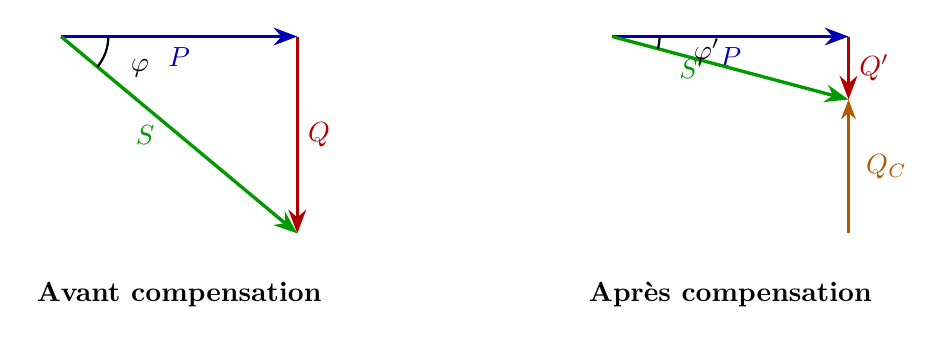
\begin{tikzpicture}[scale=1.0]
  % Triangle avant
  \begin{scope}[shift={(0,0)}]
    \draw[very thick, blue!70!black, -{Stealth[length=3mm]}] (0,0) -- (3,0) node[midway, below]{$P$};
    \draw[very thick, red!70!black, -{Stealth[length=3mm]}] (3,0) -- (3,-2.5) node[midway, right]{$Q$};
    \draw[very thick, green!60!black, -{Stealth[length=3mm]}] (0,0) -- (3,-2.5) node[midway, left=5pt]{$S$};
    \draw[thick] (0.6,0) arc[start angle=0, end angle=-40, radius=0.6];
    \node at (1,-0.4) {$\varphi$};
    \node[below] at (1.5,-3) {\textbf{Avant compensation}};
  \end{scope}
  % Triangle après
  \begin{scope}[shift={(7,0)}]
    \draw[very thick, blue!70!black, -{Stealth[length=3mm]}] (0,0) -- (3,0) node[midway, below]{$P$};
    \draw[very thick, red!70!black, -{Stealth[length=3mm]}] (3,0) -- (3,-0.8) node[midway, right]{$Q'$};
    \draw[very thick, green!60!black, -{Stealth[length=3mm]}] (0,0) -- (3,-0.8) node[midway, left=5pt]{$S'$};
    \draw[dashed, gray] (3,-0.8) -- (3,-2.5);
    \draw[very thick, orange!70!black, -{Stealth[length=2.5mm]}] (3,-2.5) -- (3,-0.8);
    \node[orange!70!black, right] at (3.1,-1.65) {$Q_C$};
    \draw[thick] (0.6,0) arc[start angle=0, end angle=-15, radius=0.6];
    \node at (1.2,-0.2) {$\varphi'$};
    \node[below] at (1.5,-3) {\textbf{Après compensation}};
  \end{scope}
\end{tikzpicture}
\end{center}

\begin{formule}
Le condensateur de compensation doit fournir une puissance réactive :
\[
Q_C = Q - Q' = P(\tan\varphi - \tan\varphi')
\]
La capacité nécessaire :
\[
\boxed{C = \frac{Q_C}{\omega U^2} = \frac{P(\tan\varphi - \tan\varphi')}{\omega U^2}}
\]
\end{formule}

\begin{retenir}
\textbf{L'essentiel sur la puissance en AC :}
\begin{enumerate}[nosep]
\item $P = UI\cos\varphi$ : seule la composante en phase produit du travail.
\item $Q = UI\sin\varphi$ : énergie ``ping-pong'' entre source et éléments réactifs.
\item $S^2 = P^2 + Q^2$ : le réseau fournit la puissance apparente $S$.
\item $\cos\varphi < 1$ $\Rightarrow$ courant surdimensionné $\Rightarrow$ pertes et surcoûts.
\item Compensation : condensateurs en parallèle pour les charges inductives.
\end{enumerate}
\end{retenir}

% ----------------------------------------------------------------------------
\section{Approfondissement}

\begin{approfondissement}
Puissance complexe, triangle des puissances, et bilan de puissance complet. Prérequis : chapitre 10 (complexes).
\end{approfondissement}

\subsection{Puissance complexe}

En notation complexe, la puissance s'écrit très élégamment :

\begin{formule}
\[
\boxed{\underline{S} = \frac{1}{2}\underline{\hat{U}} \cdot \underline{\hat{I}}^* = \underline{U}_{\text{eff}} \cdot \underline{I}_{\text{eff}}^* = P + jQ}
\]
\begin{itemize}[nosep]
\item $\underline{I}^*$ : conjugué de $\underline{I}$ (on inverse le signe de la phase).
\item $\text{Re}(\underline{S}) = P$ (puissance active).
\item $\text{Im}(\underline{S}) = Q$ (puissance réactive).
\item $|\underline{S}| = S$ (puissance apparente).
\end{itemize}
\end{formule}

\begin{intuition}
Pourquoi le conjugué ? Si $\underline{U} = Ue^{j0}$ et $\underline{I} = Ie^{-j\varphi}$ (courant en retard), alors $\underline{U}\cdot\underline{I}^* = UIe^{j\varphi}$. La partie réelle donne $UI\cos\varphi = P$ et la partie imaginaire $UI\sin\varphi = Q$. Sans le conjugué, les signes de $Q$ seraient inversés.
\end{intuition}

\subsection{Puissance dissipée dans chaque composant}

\begin{center}
\renewcommand{\arraystretch}{1.5}
\begin{tabular}{lcccl}
\toprule
\textbf{Composant} & $\underline{Z}$ & $\varphi$ & $P$ & $Q$ \\
\midrule
Résistance $R$ & $R$ & $0°$ & $RI^2$ & $0$ \\
Inductance $L$ & $j\omega L$ & $+90°$ & $0$ & $+\omega LI^2$ (consomme) \\
Condensateur $C$ & $1/(j\omega C)$ & $-90°$ & $0$ & $-U^2\omega C$ (fournit) \\
\bottomrule
\end{tabular}
\end{center}

\textbf{Interprétation :} seule la résistance consomme de la puissance active. $L$ et $C$ ne font qu'échanger de la puissance réactive avec la source (avec des signes opposés : c'est pourquoi un condensateur peut compenser une inductance).

\subsection{Bilan de puissance d'un circuit AC}

Comme en DC, la conservation de l'énergie s'applique, mais séparément pour $P$ et $Q$ :

\begin{formule}
\[
\boxed{\sum P_{\text{fournie}} = \sum P_{\text{consommée}}} \qquad \boxed{\sum Q_{\text{fournie}} = \sum Q_{\text{consommée}}}
\]
Les puissances actives s'équilibrent. Les puissances réactives aussi. Mais on ne peut \textit{pas} additionner $P$ et $Q$ directement (ce sont des composantes orthogonales).
\end{formule}

\subsection{Exemple complet : circuit RL + compensation}

\textbf{Données :} $U = \SI{230}{V}$ eff, $f = \SI{50}{Hz}$. Charge : $R = \SI{20}{\ohm}$ en série avec $L = \SI{50}{mH}$.

\textbf{Avant compensation :}

$\underline{Z} = R + j\omega L = 20 + j\times2\pi\times50\times0{,}05 = 20 + j\SI{15.7}{\ohm}$.

$|Z| = \sqrt{20^2 + 15{,}7^2} = \SI{25.4}{\ohm}$.

$I = U/|Z| = 230/25{,}4 = \SI{9.06}{A}$.

$\varphi = \arctan(15{,}7/20) = 38{,}1°$. $\cos\varphi = 0{,}786$.

$P = UI\cos\varphi = 230\times9{,}06\times0{,}786 = \SI{1638}{W}$.

$Q = UI\sin\varphi = 230\times9{,}06\times0{,}618 = \SI{1288}{var}$.

$S = UI = \SI{2084}{VA}$.

\textbf{Compensation à $\cos\varphi' = 0{,}95$ :}

$Q' = P\tan(\arccos 0{,}95) = 1638\times0{,}329 = \SI{539}{var}$.

$Q_C = Q - Q' = 1288 - 539 = \SI{749}{var}$.

$C = Q_C/(\omega U^2) = 749/(2\pi\times50\times230^2) = \SI{45.1}{\micro F}$.

Nouveau courant : $I' = S'/U = P/(U\cos\varphi') = 1638/(230\times0{,}95) = \SI{7.5}{A}$ (au lieu de \SI{9.06}{A}).

% ----------------------------------------------------------------------------
\section{Niveau Ingénieur}

\begin{ingenieur}
Puissance en régime non sinusoïdal, harmoniques, PFC actif, et systèmes triphasés.
\end{ingenieur}

\subsection{Facteur de puissance en régime non sinusoïdal}

En présence d'\textbf{harmoniques} (redresseurs, alimentations à découpage, variateurs\ldots), le courant n'est plus sinusoïdal. Le facteur de puissance total est alors :

\begin{formule}
\[
\boxed{\text{PF} = \frac{P}{S} = \frac{P}{U_{\text{eff}} \cdot I_{\text{eff}}}}
\]
On peut le décomposer : $\text{PF} = \cos\varphi_1 \times \dfrac{I_1}{I_{\text{eff}}} = \cos\varphi_1 \times \dfrac{1}{\sqrt{1 + \text{THD}_I^2}}$

\begin{itemize}[nosep]
\item $\cos\varphi_1$ : facteur de \textbf{déplacement} (déphasage du fondamental).
\item $I_1/I_{\text{eff}}$ : facteur de \textbf{distorsion} (lié au taux de distorsion harmonique THD).
\end{itemize}
\end{formule}

\begin{attention}
Un pont redresseur classique (diodes) a un $\cos\varphi_1 \approx 1$ (le fondamental est en phase) mais un THD $\sim 80\%$. Le facteur de puissance réel n'est que $\text{PF} \approx 0{,}55$ ! Les condensateurs de compensation ne corrigent \textit{pas} ce problème --- il faut un PFC actif.
\end{attention}

\subsection{Correction active du facteur de puissance (PFC)}

Un étage PFC est un convertisseur boost commandé en courant qui force le courant d'entrée à suivre la forme de la tension (sinusoïdale). Résultat : $\text{PF} > 0{,}99$, THD $< 5\%$.

\begin{pratique}
\textbf{Obligatoire} pour les appareils $> \SI{75}{W}$ (norme IEC 61000-3-2). C'est pourquoi tous les chargeurs de PC portable, alimentations ATX, et éclairages LED de puissance intègrent un étage PFC.

Topologies courantes : boost PFC (le plus répandu), bridgeless PFC (haut rendement), totem-pole PFC (GaN, dernière génération).
\end{pratique}

\subsection{Puissance en triphasé}

En système triphasé \textbf{équilibré} (3 phases de même amplitude, déphasées de $120°$) :

\begin{formule}
\[
\boxed{P = \sqrt{3}\,U_L\,I_L\,\cos\varphi} \qquad \boxed{Q = \sqrt{3}\,U_L\,I_L\,\sin\varphi}
\]
\begin{itemize}[nosep]
\item $U_L$ : tension composée (entre phases). Ex : \SI{400}{V} en Europe.
\item $I_L$ : courant de ligne.
\item Relation : $U_L = \sqrt{3}\,V_{\text{phase}}$ (ex : $400 = \sqrt{3}\times230$).
\end{itemize}
\end{formule}

\begin{intuition}
Le triphasé transporte $\sqrt{3} \approx 1{,}73$ fois plus de puissance qu'un monophasé avec les mêmes câbles. C'est pourquoi il est utilisé systématiquement en industrie et pour le transport d'énergie.

Autre avantage : en triphasé équilibré, la puissance instantanée totale est \textbf{constante} (pas d'oscillation à $2f$). Les moteurs triphasés tournent donc sans à-coups, contrairement aux monophasés qui vibrent à \SI{100}{Hz}.
\end{intuition}

\subsection{Méthode des deux wattmètres}

En triphasé 3 fils (sans neutre), on peut mesurer la puissance active totale avec \textbf{seulement deux wattmètres} :
\[
P = W_1 + W_2 \qquad Q = \sqrt{3}(W_1 - W_2)
\]

C'est la méthode d'Aron, standard en mesure industrielle. Elle fonctionne même en charge déséquilibrée.

% === EXERCICES DU CHAPITRE 11 ===
\section*{Exercices}
\addcontentsline{toc}{section}{Exercices}

\subsection*{Niveau débutant}

\textbf{Exercice 11.1 ---} Un appareil électrique consomme \SI{1500}{W} sous \SI{230}{V} avec $\cos\varphi = 1$. Quel courant tire-t-il ? Même question avec $\cos\varphi = 0{,}6$.

\begin{pratique}
\textbf{Solution :} Avec $\cos\varphi = 1$ : $I = P/(U\cos\varphi) = 1500/230 = \SI{6.5}{A}$.

Avec $\cos\varphi = 0{,}6$ : $I = 1500/(230\times0{,}6) = \SI{10.9}{A}$.

Le courant est $67\%$ plus élevé pour la même puissance utile ! Le câblage et la protection doivent être dimensionnés en conséquence.
\end{pratique}

\textbf{Exercice 11.2 ---} Un moteur consomme $P = \SI{3}{kW}$, $Q = \SI{4}{kvar}$. Calculez $S$, $\cos\varphi$ et le courant sous \SI{400}{V}.

\begin{pratique}
\textbf{Solution :} $S = \sqrt{P^2+Q^2} = \sqrt{9+16} = \SI{5}{kVA}$.

$\cos\varphi = P/S = 3/5 = 0{,}6$. $I = S/U = 5000/400 = \SI{12.5}{A}$.
\end{pratique}

\subsection*{Niveau intermédiaire}

\textbf{Exercice 11.3 ---} Un atelier comprend : un moteur ($P_1 = \SI{5}{kW}$, $\cos\varphi_1 = 0{,}8$ inductif), un four ($P_2 = \SI{3}{kW}$, $\cos\varphi_2 = 1$), et un éclairage fluorescent ($P_3 = \SI{1}{kW}$, $\cos\varphi_3 = 0{,}5$ inductif). Calculez $P$, $Q$, $S$ et $\cos\varphi$ totaux. Quelle capacité de condensateur faut-il pour remonter à $\cos\varphi = 0{,}93$ ? ($U = \SI{230}{V}$, $f = \SI{50}{Hz}$.)

\begin{pratique}
\textbf{Solution :}

$Q_1 = P_1\tan(\arccos 0{,}8) = 5000\times0{,}75 = \SI{3750}{var}$.

$Q_2 = 0$ (résistif). $Q_3 = 1000\times\tan(\arccos 0{,}5) = 1000\times1{,}732 = \SI{1732}{var}$.

$P = 5+3+1 = \SI{9}{kW}$. $Q = 3750+0+1732 = \SI{5482}{var}$.

$S = \sqrt{9000^2+5482^2} = \SI{10539}{VA}$. $\cos\varphi = 9000/10539 = 0{,}854$.

Objectif $\cos\varphi' = 0{,}93$ : $Q' = 9000\times\tan(\arccos 0{,}93) = 9000\times0{,}395 = \SI{3559}{var}$.

$Q_C = 5482 - 3559 = \SI{1923}{var}$.

$C = Q_C/(\omega U^2) = 1923/(2\pi\times50\times230^2) = \SI{115.6}{\micro F}$.
\end{pratique}

\textbf{Exercice 11.4 ---} Démontrez que la puissance dissipée dans un condensateur pur est nulle, en calculant $P = \frac{1}{T}\int_0^T p(t)\,\mathrm{d}t$ pour $u = \hat{U}\cos\omega t$ et $i = C\omega\hat{U}\cos(\omega t + \pi/2)$.

\begin{pratique}
\textbf{Solution :} $p(t) = \hat{U}\cos(\omega t) \times C\omega\hat{U}\cos(\omega t + \pi/2)$

$= C\omega\hat{U}^2\cos(\omega t)[-\sin(\omega t)] = -\frac{1}{2}C\omega\hat{U}^2\sin(2\omega t)$.

$P = \frac{1}{T}\int_0^T -\frac{1}{2}C\omega\hat{U}^2\sin(2\omega t)\,\mathrm{d}t = 0$ \checkmark{} (moyenne d'un sinus sur une période).

Le condensateur ne consomme aucune puissance active. Toute l'énergie absorbée pendant un quart de période est restituée au quart de période suivant.
\end{pratique}

\subsection*{Niveau ingénieur}

\textbf{Exercice 11.5 ---} Un pont redresseur à diodes (sans PFC) tire un courant dont le fondamental est $I_1 = \SI{8}{A}$ en phase avec la tension ($\cos\varphi_1 = 1$), mais le THD du courant est de $80\%$. Calculez le courant efficace total, le facteur de puissance réel, et la puissance apparente sous \SI{230}{V}. Comparez avec un appareil de même puissance active mais avec PFC ($\text{PF} = 0{,}99$).

\begin{pratique}
\textbf{Solution :} $I_{\text{eff}} = I_1\sqrt{1+\text{THD}^2} = 8\sqrt{1+0{,}64} = 8\times1{,}281 = \SI{10.25}{A}$.

$P = UI_1\cos\varphi_1 = 230\times8\times1 = \SI{1840}{W}$.

$S = UI_{\text{eff}} = 230\times10{,}25 = \SI{2358}{VA}$.

$\text{PF} = P/S = 1840/2358 = 0{,}78$.

Avec PFC ($\text{PF} = 0{,}99$) : $I = P/(U\times\text{PF}) = 1840/(230\times0{,}99) = \SI{8.08}{A}$.

Économie : $10{,}25 - 8{,}08 = \SI{2.17}{A}$ de courant inutile supprimé, pertes Joule réduites de $38\%$.
\end{pratique}

\textbf{Exercice 11.6 ---} Un moteur triphasé consomme $P = \SI{15}{kW}$ avec $\cos\varphi = 0{,}75$ sous $U_L = \SI{400}{V}$. Calculez le courant de ligne. On veut $\cos\varphi' = 0{,}95$. Calculez la capacité de chaque condensateur (montage étoile).

\begin{pratique}
\textbf{Solution :} $I_L = P/(\sqrt{3}\,U_L\cos\varphi) = 15000/(\sqrt{3}\times400\times0{,}75) = \SI{28.9}{A}$.

$Q = P\tan\varphi = 15000\times\tan(\arccos 0{,}75) = 15000\times0{,}882 = \SI{13.2}{kvar}$.

$Q' = 15000\times\tan(\arccos 0{,}95) = \SI{4.93}{kvar}$.

$Q_C = 13{,}2 - 4{,}93 = \SI{8.3}{kvar}$ (total triphasé, $\SI{2.77}{kvar}$ par phase).

En montage étoile, chaque condensateur voit $V_{\text{phase}} = 400/\sqrt{3} = \SI{231}{V}$ :

$C = Q_{\text{phase}}/(\omega V_{\text{phase}}^2) = 2770/(2\pi\times50\times231^2) = \SI{165}{\micro F}$ par phase.

Nouveau courant : $I' = 15000/(\sqrt{3}\times400\times0{,}95) = \SI{22.8}{A}$ (économie de $21\%$).
\end{pratique}

\subsection*{Questions de compréhension}

\begin{enumerate}[nosep]
\item Une bobine idéale consomme-t-elle de la puissance active ? Justifiez à l'aide du déphasage.
\item Pourquoi la puissance instantanée oscille-t-elle à la fréquence $2f$ et non $f$ ?
\item Un condensateur de compensation améliore le $\cos\varphi$ mais ne réduit pas la puissance active consommée. Pourquoi l'usine économise-t-elle quand même de l'argent ?
\item Pourquoi un pont redresseur à diodes a-t-il un mauvais facteur de puissance malgré un fondamental en phase avec la tension ?
\end{enumerate}

% === RÉSUMÉ ===
\section*{Résumé du chapitre}
\addcontentsline{toc}{section}{Résumé du chapitre}

\begin{bases}[title={\color{white} Résumé --- Les Bases}]
\begin{center}
\renewcommand{\arraystretch}{1.3}
\begin{tabular}{p{4cm}p{9cm}}
\toprule
Puissance active & $P = UI\cos\varphi$ (W) --- travail utile \\
Puissance réactive & $Q = UI\sin\varphi$ (var) --- énergie oscillante \\
Puissance apparente & $S = UI$ (VA) --- $S^2 = P^2 + Q^2$ \\
$\cos\varphi$ & $P/S$ --- efficacité du transfert \\
Compensation & Condensateurs en parallèle pour charges inductives \\
\bottomrule
\end{tabular}
\end{center}
\end{bases}

\begin{approfondissement}[title={\color{white} Résumé --- Approfondissement}]
\begin{center}
\renewcommand{\arraystretch}{1.3}
\begin{tabular}{p{4cm}p{9cm}}
\toprule
$\underline{S}$ complexe & $\underline{S} = \underline{U}\cdot\underline{I}^* = P + jQ$ \\
Bilan AC & $\sum P$ et $\sum Q$ s'équilibrent séparément \\
Par composant & $R$ : $P = RI^2$, $Q=0$ ; $L$ : $Q > 0$ ; $C$ : $Q < 0$ \\
\bottomrule
\end{tabular}
\end{center}
\end{approfondissement}

\begin{ingenieur}[title={\color{white} Résumé --- Niveau Ingénieur}]
\begin{center}
\renewcommand{\arraystretch}{1.3}
\begin{tabular}{p{4cm}p{9cm}}
\toprule
Non sinusoïdal & $\text{PF} = \cos\varphi_1 / \sqrt{1+\text{THD}^2}$ --- PFC actif obligatoire $>\SI{75}{W}$ \\
Triphasé & $P = \sqrt{3}\,U_L I_L \cos\varphi$ --- puissance constante \\
Wattmètres & Méthode d'Aron : 2 wattmètres suffisent en 3 fils \\
\bottomrule
\end{tabular}
\end{center}
\end{ingenieur}

% ============================================================================
% CHAPITRE 12 : RÉSONANCE
% ============================================================================
\chapter{Résonance}

\begin{center}
\textit{La résonance est le phénomène par lequel un circuit amplifie\\
sélectivement une fréquence parmi toutes les autres.\\
C'est la clé de la radio, des filtres, des oscillateurs et des horloges.}
\end{center}

\vspace{0.5cm}

Le chapitre 9 a introduit la fréquence propre $f_0 = 1/(2\pi\sqrt{LC})$ et le facteur de qualité $Q$. Le chapitre 10 a donné les outils complexes. Ce chapitre réunit tout pour étudier en détail ce qui se passe quand on \textbf{excite un circuit RLC à sa fréquence propre} --- et au voisinage.

% ----------------------------------------------------------------------------
\section{Les Bases}

\begin{bases}
La résonance est un phénomène universel : une corde de guitare, un verre de cristal, une balançoire, la radio FM\ldots{} Dans tous les cas, le principe est le même : un système oscille avec une grande amplitude quand on l'excite à ``sa'' fréquence. Prérequis : chapitres 9 et 10.
\end{bases}

\subsection{Le phénomène de résonance : intuition}

\begin{analogie}
\textbf{La balançoire.} Pour qu'une balançoire atteigne une grande amplitude, il faut la pousser \textit{au bon rythme} --- exactement à sa fréquence naturelle de balancement. Si vous poussez trop vite ou trop lentement, l'amplitude reste faible. Si vous poussez pile au bon moment à chaque oscillation, l'amplitude \textbf{s'accumule} à chaque cycle.

En électronique : la ``balançoire'' est le circuit LC. La ``poussée'' est la source sinusoïdale. La ``fréquence naturelle'' est $f_0 = 1/(2\pi\sqrt{LC})$. Et le ``frottement de l'air'' qui empêche l'amplitude de devenir infinie, c'est la résistance $R$.
\end{analogie}

\subsection{Pourquoi l'inductance et le condensateur se compensent}

À la fréquence $f_0$, un phénomène remarquable se produit. Rappelons les impédances (chapitre 10) :
\begin{itemize}[nosep]
\item Condensateur : $\underline{Z}_C = 1/(j\omega C) = -j/(\omega C)$. Impédance \textbf{imaginaire négative}.
\item Bobine : $\underline{Z}_L = j\omega L$. Impédance \textbf{imaginaire positive}.
\end{itemize}

À la fréquence $f_0$, on a $\omega_0 = 1/\sqrt{LC}$, donc $\omega_0 L = 1/(\omega_0 C)$. Les deux impédances réactives ont le \textbf{même module et des signes opposés} :
\[
\underline{Z}_L + \underline{Z}_C = j\omega_0 L - \frac{j}{\omega_0 C} = j\omega_0 L - j\omega_0 L = 0
\]

\begin{intuition}
\textbf{Les deux composants ``s'annulent'' mutuellement.} L'inductance et le condensateur échangent de l'énergie entre eux (magnétique $\leftrightarrow$ électrique) à chaque demi-cycle, sans demander d'énergie à la source. Seule la résistance dissipe de l'énergie, et c'est elle qui limite l'amplitude à la résonance.
\end{intuition}

\begin{formule}
\[
\boxed{f_0 = \frac{1}{2\pi\sqrt{LC}}} \qquad \boxed{\omega_0 = \frac{1}{\sqrt{LC}}}
\]
C'est la \textbf{fréquence de résonance}. Elle ne dépend que de $L$ et $C$, pas de $R$.
\end{formule}

\subsection{Résonance série}

Considérons un circuit RLC série alimenté par une source sinusoïdale $\underline{E}$ de fréquence variable :

\begin{center}
\begin{circuitikz}[scale=0.85]
  \draw (0,0) to[sinusoidal voltage source, l=$e(t)$] (0,3)
        to[R, l=$R$] (2.5,3)
        to[L, l=$L$] (5,3)
        to[C, l=$C$] (5,0) -- (0,0);
  \draw[line width=1.2pt, blue!70!black, -{Stealth[length=2.5mm]}] (0.3,3.3) -- (1.8,3.3);
  \node[blue!70!black, above, font=\small] at (1.05,3.3) {$i$};
\end{circuitikz}
\end{center}

L'impédance totale est $\underline{Z} = R + j(\omega L - 1/(\omega C))$.

\begin{formule}
\textbf{À la résonance} ($f = f_0$) :
\begin{itemize}[nosep]
\item L'impédance est \textbf{minimale et purement réelle} : $|\underline{Z}| = R$.
\item Le courant est \textbf{maximal} : $I = E/R$.
\item Tension et courant sont \textbf{en phase} ($\varphi = 0$).
\end{itemize}
\end{formule}

\begin{attention}
\textbf{Surtension à la résonance :} à $f_0$, les tensions aux bornes de $L$ et de $C$ sont individuellement \textbf{bien supérieures} à la tension source :
\[
\boxed{U_L = U_C = Q \times E}
\]
Si $Q = 50$ et $E = \SI{1}{V}$, alors $U_L = U_C = \SI{50}{V}$ ! Ces deux tensions sont égales en module mais \textbf{opposées en phase} : elles se compensent aux bornes de la série, mais existent bel et bien individuellement.

\textbf{C'est dangereux :} un condensateur ou un fil de bobine peut claquer sous cette surtension. Toujours vérifier la tenue en tension des composants dans un circuit résonant.
\end{attention}

\subsection{Résonance parallèle}

Dans un circuit RLC parallèle (les trois composants entre les mêmes deux n\oe uds) :

\begin{center}
\begin{circuitikz}[scale=0.85]
  \draw (0,0) to[sinusoidal voltage source, l=$e(t)$] (0,3) -- (1.5,3);
  \draw (1.5,3) -- (1.5,2.5) to[R, l=$R$] (1.5,0.5) -- (1.5,0);
  \draw (3,3) -- (3,2.5) to[L, l=$L$] (3,0.5) -- (3,0);
  \draw (4.5,3) -- (4.5,2.5) to[C, l=$C$] (4.5,0.5) -- (4.5,0);
  \draw (1.5,3) -- (4.5,3);
  \draw (0,0) -- (4.5,0);
\end{circuitikz}
\end{center}

\begin{formule}
\textbf{À la résonance} ($f = f_0$) :
\begin{itemize}[nosep]
\item L'impédance est \textbf{maximale} : $|\underline{Z}| = R$ (pour un RLC parallèle idéal).
\item Le courant total tiré à la source est \textbf{minimal}.
\item Les courants dans $L$ et $C$ sont $Q$ fois supérieurs au courant total, mais \textbf{en opposition de phase} : ils se compensent en se ``refermant'' entre $L$ et $C$ sans passer par la source.
\end{itemize}
\end{formule}

\begin{intuition}
\textbf{Série vs parallèle :} la résonance série ``aspire'' le courant (impédance minimale = court-circuit résonant). La résonance parallèle ``bloque'' le courant (impédance maximale = circuit bouchon). Ce sont des comportements \textbf{duaux}.

\begin{center}
\begin{tabular}{lcc}
\toprule
 & \textbf{Résonance série} & \textbf{Résonance parallèle} \\
\midrule
$|\underline{Z}|$ à $f_0$ & Minimale ($= R$) & Maximale ($= R_p$) \\
Courant & Maximal & Minimal \\
Surtension interne & $U_L = U_C = QE$ & $I_L = I_C = QI$ (surcourant) \\
Application & Filtre passe-bande & Circuit bouchon (réjecteur) \\
\bottomrule
\end{tabular}
\end{center}
\end{intuition}

\subsection{Bande passante et sélectivité}

Un circuit résonant ne répond pas \textit{uniquement} à $f_0$ : il répond aussi aux fréquences voisines, mais avec une amplitude moindre. La \textbf{bande passante} $\Delta f$ est la plage de fréquences pour laquelle la réponse reste au-dessus de $-3$ dB (soit $1/\sqrt{2}$ du maximum).

\begin{formule}
\[
\boxed{\Delta f = \frac{f_0}{Q}} \qquad \text{ou} \qquad \boxed{Q = \frac{f_0}{\Delta f}}
\]
\begin{itemize}[nosep]
\item $Q$ élevé $\Rightarrow$ $\Delta f$ petit $\Rightarrow$ haute sélectivité (le circuit ``trie'' finement les fréquences).
\item $Q$ faible $\Rightarrow$ $\Delta f$ grand $\Rightarrow$ faible sélectivité (le circuit laisse passer une large bande).
\end{itemize}
\end{formule}

\begin{pratique}
\textbf{Application : la radio.} Le principe d'un récepteur radio (AM ou FM) est un circuit LC résonant accordable :
\begin{itemize}[nosep]
\item On fait varier $C$ (condensateur variable, ou varicap commandé en tension) pour changer $f_0$.
\item Le circuit sélectionne la station dont la fréquence correspond à $f_0$.
\item La bande passante $\Delta f$ doit être assez large pour laisser passer le signal modulé ($\sim\SI{10}{kHz}$ en AM, $\sim\SI{200}{kHz}$ en FM), mais assez étroite pour rejeter les stations voisines.
\end{itemize}
Pour la bande AM ($f_0 \sim \SI{1}{MHz}$, $\Delta f = \SI{10}{kHz}$) : $Q = 10^6/10^4 = 100$. Pour la FM ($f_0 \sim \SI{100}{MHz}$, $\Delta f = \SI{200}{kHz}$) : $Q = 10^8/2\times10^5 = 500$.
\end{pratique}

\begin{retenir}
\textbf{L'essentiel sur la résonance :}
\begin{enumerate}[nosep]
\item Résonance quand $L$ et $C$ se compensent : $f_0 = 1/(2\pi\sqrt{LC})$.
\item Série : $|Z|$ minimale $= R$, courant maximal, surtension $QE$ sur $L$ et $C$.
\item Parallèle : $|Z|$ maximale, courant minimal (circuit bouchon).
\item Sélectivité : $\Delta f = f_0/Q$. Plus $Q$ est grand, plus c'est sélectif.
\item $Q$ ne dépend que du rapport énergie stockée / énergie dissipée par cycle.
\end{enumerate}
\end{retenir}

% ----------------------------------------------------------------------------
\section{Approfondissement}

\begin{approfondissement}
Courbes d'impédance et de gain, calculs détaillés, et circuits résonants pratiques. Prérequis : chapitre 10 (notation complexe).
\end{approfondissement}

\subsection{Impédance du circuit RLC série en fonction de la fréquence}

\[
\underline{Z}(\omega) = R + j\left(\omega L - \frac{1}{\omega C}\right)
\]

\textbf{Module :}
\[
|Z(\omega)| = \sqrt{R^2 + \left(\omega L - \frac{1}{\omega C}\right)^2}
\]

On peut écrire sous forme normalisée en posant $x = \omega/\omega_0 = f/f_0$ :
\[
|Z| = R\sqrt{1 + Q^2\left(x - \frac{1}{x}\right)^2}
\]

\begin{center}
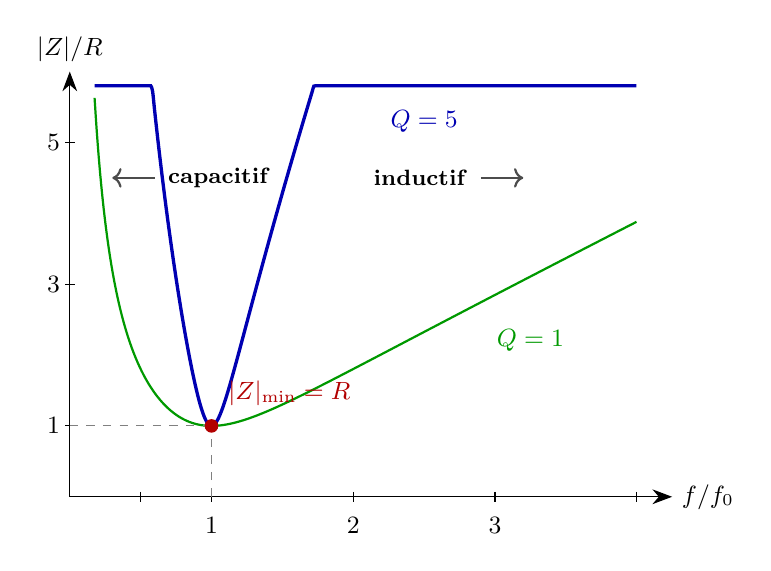
\begin{tikzpicture}[scale=0.9]
  % Axes
  \draw[-{Stealth[length=2.5mm]}] (0,0) -- (8.5,0) node[right]{\small $f/f_0$};
  \draw[-{Stealth[length=2.5mm]}] (0,0) -- (0,6) node[above]{\small $|Z|/R$};
  
  % Graduations axe x
  \foreach \x/\lab in {1/0.5, 2/1, 4/2, 6/3, 8/4} {
    \draw (\x,0.07) -- (\x,-0.07);
  }
  \node[below, font=\small] at (2,-0.15) {$1$};
  \node[below, font=\small] at (4,-0.15) {$2$};
  \node[below, font=\small] at (6,-0.15) {$3$};
  
  % Graduations axe y
  \node[left, font=\small] at (0,1) {$1$};
  \draw (0.07,1) -- (-0.07,1);
  \node[left, font=\small] at (0,3) {$3$};
  \draw (0.07,3) -- (-0.07,3);
  \node[left, font=\small] at (0,5) {$5$};
  \draw (0.07,5) -- (-0.07,5);
  
  % Courbe Q = 1 (x en unités de graphe : x_graph = 2*f/f0, donc f/f0 = x_graph/2)
  % |Z|/R = sqrt(1 + Q^2 * (f/f0 - f0/f)^2)
  % Avec x_graph: f/f0 = x_graph/2, donc (f/f0 - f0/f) = (x/2 - 2/x)
  \draw[thick, green!60!black, domain=0.35:8, samples=300, smooth]
    plot(\x, {min(5.8, sqrt(1 + 1*(\x/2 - 2/\x)*(\x/2 - 2/\x)))});
  \node[green!60!black, font=\small\bfseries] at (6.5,2.2) {$Q = 1$};
  
  % Courbe Q = 5
  \draw[very thick, blue!70!black, domain=0.35:8, samples=300, smooth]
    plot(\x, {min(5.8, sqrt(1 + 25*(\x/2 - 2/\x)*(\x/2 - 2/\x)))});
  \node[blue!70!black, font=\small\bfseries] at (5,5.3) {$Q = 5$};
  
  % Minimum à f/f0 = 1
  \draw[dashed, gray] (2,0) -- (2,1);
  \draw[dashed, gray] (0,1) -- (2,1);
  \filldraw[red!70!black] (2,1) circle (2.5pt);
  \node[red!70!black, above right, font=\small] at (2.1,1.15) {$|Z|_{\min} = R$};
  
  % Annotations régions
  \draw[<-, thick, gray!60!black] (0.6,4.5) -- (1.2,4.5);
  \node[font=\footnotesize, right] at (1.25,4.5) {\textbf{capacitif}};
  \draw[->, thick, gray!60!black] (5.8,4.5) -- (6.4,4.5);
  \node[font=\footnotesize, left] at (5.75,4.5) {\textbf{inductif}};
\end{tikzpicture}
\end{center}

\textbf{Comportement asymptotique :}
\begin{itemize}[nosep]
\item \textbf{$f \ll f_0$} : $|Z| \approx 1/(\omega C)$. Le condensateur domine. Le circuit est \textbf{capacitif}.
\item \textbf{$f = f_0$} : $|Z| = R$. Minimum. Le circuit est \textbf{purement résistif}.
\item \textbf{$f \gg f_0$} : $|Z| \approx \omega L$. L'inductance domine. Le circuit est \textbf{inductif}.
\end{itemize}

\subsection{Fonction de transfert du filtre passe-bande}

Si on prend la tension aux bornes de $R$ comme sortie (dans le RLC série), on obtient un filtre \textbf{passe-bande} :

\begin{formule}
\[
\underline{H}(\omega) = \frac{R}{\underline{Z}} = \frac{1}{1 + jQ\left(\dfrac{\omega}{\omega_0} - \dfrac{\omega_0}{\omega}\right)}
\]

\textbf{Gain :} $|H| = \dfrac{1}{\sqrt{1 + Q^2\left(\dfrac{f}{f_0} - \dfrac{f_0}{f}\right)^2}}$

\textbf{Phase :} $\varphi = -\arctan\left[Q\left(\dfrac{f}{f_0} - \dfrac{f_0}{f}\right)\right]$
\end{formule}

\begin{center}
\begin{tabular}{lll}
\toprule
\textbf{Fréquence} & \textbf{Gain $|H|$} & \textbf{Phase $\varphi$} \\
\midrule
$f \ll f_0$ & $\to 0$ (atténuation BF) & $\to +90°$ \\
$f = f_0$ & $1$ (gain maximal) & $0°$ \\
$f \gg f_0$ & $\to 0$ (atténuation HF) & $\to -90°$ \\
\bottomrule
\end{tabular}
\end{center}

Le filtre laisse passer les fréquences autour de $f_0$ et atténue le reste. La largeur de la bande passante est $\Delta f = f_0/Q$.

\subsection{Les autres fonctions de transfert du RLC série}

Le même circuit RLC série donne des filtres \textit{différents} selon le composant aux bornes duquel on prend la sortie :

\begin{center}
\begin{tabular}{lll}
\toprule
\textbf{Sortie aux bornes de} & \textbf{Type de filtre} & \textbf{Gain à $f_0$} \\
\midrule
$R$ & \textbf{Passe-bande} & $|H| = 1$ \\
$C$ & \textbf{Passe-bas} (2nd ordre) & $|H| = Q$ (surtension si $Q > 1$) \\
$L$ & \textbf{Passe-haut} (2nd ordre) & $|H| = Q$ (surtension) \\
$L + C$ & \textbf{Coupe-bande} (réjecteur) & $|H| = 0$ (zéro de transmission) \\
\bottomrule
\end{tabular}
\end{center}

\begin{attention}
\textbf{Piège :} le ``filtre passe-bas'' aux bornes de $C$ a un gain $> 1$ à $f_0$ si $Q > 1$. Ce n'est pas une amplification (le circuit est passif) : c'est la surtension de résonance. Le gain \textit{maximal} ne se produit pas exactement à $f_0$ mais légèrement en dessous (pour $Q > 1/\sqrt{2}$). Cette distinction est souvent source de confusion.
\end{attention}

\subsection{Circuit bouchon (résonance parallèle)}

L'admittance du RLC parallèle est :
\[
\underline{Y}(\omega) = \frac{1}{R} + j\left(\omega C - \frac{1}{\omega L}\right)
\]

À la résonance : $\omega_0 C = 1/(\omega_0 L)$, donc $\underline{Y} = 1/R$ et $|\underline{Z}| = R$ (maximum).

\begin{pratique}
\textbf{Application : filtre réjecteur de bande (notch).} Un circuit bouchon en \textbf{série} avec le signal bloque la fréquence $f_0$ et laisse passer le reste. Usage typique : éliminer le \SI{50}{Hz} parasite dans un amplificateur audio ou un ECG médical.

Un circuit bouchon en \textbf{parallèle} avec le signal sélectionne $f_0$ et atténue le reste. Usage typique : circuit d'accord d'un récepteur radio.
\end{pratique}

\subsection{Calcul pratique : dimensionnement d'un circuit résonant}

\begin{pratique}
\textbf{Exemple complet :} on veut un filtre passe-bande centré sur $f_0 = \SI{455}{kHz}$ (fréquence intermédiaire standard en radio AM) avec une bande passante de $\SI{10}{kHz}$.

\textbf{1. Facteur de qualité :} $Q = f_0/\Delta f = 455/10 = 45{,}5$.

\textbf{2. Choix de $C$ :} prenons $C = \SI{100}{pF}$ (valeur courante en RF).

\textbf{3. Calcul de $L$ :} $L = 1/(\omega_0^2 C) = 1/((2\pi\times455\times10^3)^2\times10^{-10})$

$= 1/(8{,}17\times10^{12}\times10^{-10}) = 1/817 \approx \SI{1.22}{mH}$.

\textbf{4. Calcul de $R$ :} $R = (1/Q)\sqrt{L/C} = (1/45{,}5)\sqrt{1{,}22\times10^{-3}/10^{-10}}$

$= (1/45{,}5)\times\sqrt{1{,}22\times10^7} = (1/45{,}5)\times3493 \approx \SI{76.8}{\ohm}$.

\textbf{Vérification :} $R$ doit être la résistance \textit{totale} du circuit (résistance du fil de la bobine + résistance de la source + charge). Si la bobine a $R_{\text{bobine}} = \SI{50}{\ohm}$, il reste $\SI{26.8}{\ohm}$ pour la source et la charge.
\end{pratique}

% ----------------------------------------------------------------------------
\section{Niveau Ingénieur}

\begin{ingenieur}
Facteur de qualité en charge, résonateurs réels, transformation d'impédance, et applications avancées.
\end{ingenieur}

\subsection{$Q$ intrinsèque, $Q$ en charge, et $Q$ externe}

En pratique, un circuit résonant est toujours connecté à une source (résistance interne $R_s$) et à une charge ($R_L$). Le $Q$ effectif (``loaded $Q$'' ou $Q_L$) est toujours inférieur au $Q$ intrinsèque ($Q_0$, ou ``unloaded $Q$'') :

\begin{formule}
\[
\boxed{\frac{1}{Q_L} = \frac{1}{Q_0} + \frac{1}{Q_{\text{ext}}}}
\]
\begin{itemize}[nosep]
\item $Q_0$ : facteur de qualité \textit{du résonateur seul} (limité par les pertes internes : résistance du fil, pertes du noyau, ESR du condensateur).
\item $Q_{\text{ext}}$ : facteur de qualité \textit{externe} (dû au couplage avec la source et la charge).
\item $Q_L$ : facteur de qualité \textit{effectif} en fonctionnement. C'est lui qui détermine la bande passante réelle.
\end{itemize}
\end{formule}

\begin{attention}
\textbf{Conséquence critique :} un résonateur à $Q_0 = 200$ couplé fortement à une source $50\,\Omega$ peut avoir un $Q_L$ de seulement 20. La bande passante réelle est 10 fois plus large que celle du résonateur seul. En RF, on contrôle le couplage (prise intermédiaire sur la bobine, couplage capacitif faible) pour préserver un $Q_L$ élevé.
\end{attention}

\subsection{Transformation d'impédance par circuit résonant}

Un circuit résonant parallèle de haute impédance ($R_p = Q_0^2 \times R_s$ en série) peut servir à \textbf{transformer l'impédance} entre une source et une charge. C'est le principe des \textbf{réseaux d'adaptation} en RF.

\textbf{Réseau en L (L-match) :} le réseau d'adaptation le plus simple est constitué d'un seul $L$ et d'un seul $C$. Il transforme $R_s$ en $R_L$ (ou inversement) à la fréquence $f_0$.

\begin{formule}
Pour adapter $R_s$ (faible) à $R_L$ (élevée) avec un réseau en L (série $L$ + shunt $C$) :
\[
Q_{\text{match}} = \sqrt{\frac{R_L}{R_s} - 1}
\]
\[
X_L = Q_{\text{match}} \times R_s \qquad X_C = \frac{R_L}{Q_{\text{match}}}
\]
La bande passante du réseau est $\Delta f \approx f_0/Q_{\text{match}}$.
\end{formule}

\begin{pratique}
\textbf{Exemple :} adapter une antenne de $R_s = \SI{50}{\ohm}$ à un amplificateur de $R_L = \SI{200}{\ohm}$ à $f_0 = \SI{100}{MHz}$.

$Q_{\text{match}} = \sqrt{200/50 - 1} = \sqrt{3} = 1{,}73$.

$X_L = 1{,}73 \times 50 = \SI{86.5}{\ohm}$ $\Rightarrow$ $L = X_L/\omega = 86{,}5/(2\pi\times10^8) = \SI{138}{nH}$.

$X_C = 200/1{,}73 = \SI{115.5}{\ohm}$ $\Rightarrow$ $C = 1/(\omega X_C) = 1/(2\pi\times10^8\times115{,}5) = \SI{13.8}{pF}$.

Bande passante : $\Delta f \approx 100/1{,}73 \approx \SI{58}{MHz}$ (large bande car $Q$ est faible).
\end{pratique}

\subsection{Résonateurs réels : du LC au quartz}

Les circuits LC discrets ont un $Q$ limité par les pertes dans les composants ($Q \sim 50$--$200$). Pour obtenir des $Q$ très élevés, on utilise d'autres technologies :

\begin{center}
\renewcommand{\arraystretch}{1.3}
\begin{tabular}{llll}
\toprule
\textbf{Résonateur} & \textbf{$Q$ typique} & \textbf{Gamme de $f$} & \textbf{Usage principal} \\
\midrule
LC discret & $50$--$200$ & kHz--GHz & Filtres, VCO, adaptation \\
Quartz & $10^4$--$10^5$ & kHz--\SI{200}{MHz} & Horloges, oscillateurs de référence \\
Céramique & $500$--$2000$ & MHz & Filtres IF (radio) \\
SAW & $1000$--$5000$ & MHz--GHz & Filtres RF (téléphones, GPS) \\
BAW/FBAR & $1000$--$3000$ & GHz & Filtres 5G, Wi-Fi \\
MEMS & $10^4$--$10^6$ & kHz--GHz & Oscillateurs MEMS, gyroscopes \\
Cavité métallique & $10^3$--$10^5$ & GHz & Radar, spatial, instrumentation \\
Résonateur diélectrique & $5000$--$50\,000$ & GHz & Filtres stations de base \\
\bottomrule
\end{tabular}
\end{center}

\begin{intuition}
\textbf{Pourquoi le quartz a un $Q$ si élevé ?} Le quartz est un cristal piézoélectrique : il vibre mécaniquement à une fréquence très précise, déterminée par ses dimensions. Les pertes mécaniques dans le cristal sont extrêmement faibles (bien inférieures aux pertes électriques dans un circuit LC). Électriquement, le quartz se modélise par un circuit RLC série (avec $R$ très faible) en parallèle avec une capacité $C_0$ (les armatures métalliques).

C'est pourquoi toutes les horloges numériques (montres, microcontrôleurs, ordinateurs) utilisent un oscillateur à quartz : la fréquence est stable à $\sim\SI{20}{ppm}$ (20 millionièmes) sans compensation de température.
\end{intuition}

\subsection{Résonances parasites en conception réelle}

\begin{attention}
\textbf{Les résonances non voulues sont un cauchemar en conception.} Tout circuit réel contient des inductances et capacités parasites qui forment des circuits résonants :

\textbf{1. Condensateur réel :} ESL + C $\Rightarrow$ résonance série (SRF). Au-dessus, le condensateur est inductif (chapitre 7). Un condensateur de découplage de \SI{100}{nF}/0805 résonne à $\sim\SI{30}{MHz}$.

\textbf{2. Inductance réelle :} $L$ + capacité inter-spires $\Rightarrow$ résonance parallèle. Au-dessus, l'inductance est capacitive (chapitre 8).

\textbf{3. Piste de PCB :} inductance distribuée + capacité vers le plan de masse $\Rightarrow$ résonance quart d'onde à $f = c/(4\ell)$. Une piste de \SI{5}{cm} résonne à $\sim\SI{1}{GHz}$.

\textbf{4. Plan d'alimentation :} le plan de cuivre et le plan de masse forment un condensateur plan, avec des inductances de via. Le résultat est un réseau de résonances qui peut amplifier le bruit sur le bus d'alimentation à certaines fréquences.

\textbf{Solution systématique :} amortir les résonances par des résistances (réduire $Q$), multiplier les condensateurs de découplage (couvrir toutes les fréquences), et simuler l'impédance du bus d'alimentation ($Z_{\text{PDN}}$) en phase de conception.
\end{attention}

% === EXERCICES DU CHAPITRE 12 ===
\section*{Exercices}
\addcontentsline{toc}{section}{Exercices}

\subsection*{Niveau débutant}

\textbf{Exercice 12.1 ---} Un circuit LC a $L = \SI{10}{mH}$ et $C = \SI{100}{nF}$. Calculez $f_0$. Avec $R = \SI{50}{\ohm}$, calculez $Q$ et la bande passante.

\begin{pratique}
\textbf{Solution :} $f_0 = 1/(2\pi\sqrt{10^{-2}\times10^{-7}}) = 1/(2\pi\times10^{-4{,}5} \approx 3{,}16\times10^{-5}) \approx \SI{5.03}{kHz}$.

$Q = (1/R)\sqrt{L/C} = (1/50)\sqrt{10^{-2}/10^{-7}} = (1/50)\times\sqrt{10^5} = (1/50)\times316 = 6{,}3$.

$\Delta f = f_0/Q = 5030/6{,}3 \approx \SI{798}{Hz}$.
\end{pratique}

\textbf{Exercice 12.2 ---} À la résonance, un circuit RLC série ($E = \SI{5}{V}$, $Q = 30$) génère quelle tension aux bornes du condensateur ? Est-ce dangereux pour un condensateur de $\SI{50}{V}$ ?

\begin{pratique}
\textbf{Solution :} $U_C = QE = 30\times5 = \SI{150}{V}$.

Le condensateur voit \SI{150}{V} alors que la source ne fournit que \SI{5}{V}. Pour un condensateur de \SI{50}{V} max : \textbf{destruction certaine}. Il faut un condensateur d'au moins \SI{200}{V} (avec marge).
\end{pratique}

\subsection*{Niveau intermédiaire}

\textbf{Exercice 12.3 ---} On veut un filtre passe-bande centré sur $f_0 = \SI{10}{kHz}$ avec $\Delta f = \SI{500}{Hz}$. Calculez $Q$. Si $C = \SI{10}{nF}$, déterminez $L$ et $R$.

\begin{pratique}
\textbf{Solution :} $Q = f_0/\Delta f = 10000/500 = 20$.

$L = 1/(\omega_0^2 C) = 1/((2\pi\times10^4)^2\times10^{-8}) = 1/(3{,}95\times10^{9}\times10^{-8}) = 1/39{,}5 \approx \SI{25.3}{mH}$.

$R = (1/Q)\sqrt{L/C} = (1/20)\sqrt{25{,}3\times10^{-3}/10^{-8}} = (1/20)\times\sqrt{2{,}53\times10^6}$

$= (1/20)\times1590 = \SI{79.6}{\ohm}$.
\end{pratique}

\textbf{Exercice 12.4 ---} Un récepteur radio AM doit couvrir la bande \SI{530}{kHz}--\SI{1700}{kHz} avec un circuit LC à condensateur variable. Si $L = \SI{250}{\micro H}$, quelles sont les valeurs min et max de $C$ ?

\begin{pratique}
\textbf{Solution :} $C = 1/(\omega^2 L) = 1/((2\pi f)^2 \times L)$.

$C_{\max}$ (à $f_{\min} = \SI{530}{kHz}$) : $C = 1/((2\pi\times5{,}3\times10^5)^2\times2{,}5\times10^{-4})$

$= 1/(1{,}109\times10^{13}\times2{,}5\times10^{-4}) = 1/(2{,}77\times10^9) = \SI{361}{pF}$.

$C_{\min}$ (à $f_{\max} = \SI{1700}{kHz}$) : $C = 1/((2\pi\times1{,}7\times10^6)^2\times2{,}5\times10^{-4})$

$= 1/(1{,}14\times10^{14}\times2{,}5\times10^{-4}) = 1/(2{,}85\times10^{10}) = \SI{35.1}{pF}$.

Le condensateur variable doit couvrir de \SI{35}{pF} à \SI{361}{pF}, soit un rapport $\sim 10:1$.
\end{pratique}

\subsection*{Niveau ingénieur}

\textbf{Exercice 12.5 ---} Un résonateur à quartz de \SI{10}{MHz} a $Q_0 = 80\,000$. Il est couplé à un circuit dont le $Q_{\text{ext}} = 500$. Calculez $Q_L$ et la bande passante effective. Comparez avec la bande passante intrinsèque.

\begin{pratique}
\textbf{Solution :} $1/Q_L = 1/Q_0 + 1/Q_{\text{ext}} = 1/80000 + 1/500 = 0{,}0000125 + 0{,}002 = 0{,}002$.

$Q_L \approx 498$. Le $Q$ est presque entièrement dominé par le couplage externe.

$\Delta f_L = f_0/Q_L = 10^7/498 = \SI{20.1}{kHz}$.

$\Delta f_0 = f_0/Q_0 = 10^7/80000 = \SI{125}{Hz}$.

La bande passante est passée de \SI{125}{Hz} (intrinsèque) à \SI{20}{kHz} (en charge) : un facteur 160. Le couplage a ``gaspillé'' presque tout le $Q$ du quartz.

\textbf{Morale :} pour exploiter un résonateur à haut $Q$, le couplage doit être \textit{faible} ($Q_{\text{ext}} \gg Q_0$).
\end{pratique}

\textbf{Exercice 12.6 ---} On veut adapter une source de \SI{50}{\ohm} à une charge de \SI{1000}{\ohm} à \SI{433}{MHz} (bande ISM). Calculez les composants d'un réseau en L. Quelle est la bande passante du réseau d'adaptation ?

\begin{pratique}
\textbf{Solution :} $Q_{\text{match}} = \sqrt{R_L/R_s - 1} = \sqrt{1000/50 - 1} = \sqrt{19} = 4{,}36$.

$X_L = Q_{\text{match}}\times R_s = 4{,}36\times50 = \SI{218}{\ohm}$.

$L = X_L/\omega = 218/(2\pi\times433\times10^6) = \SI{80.1}{nH}$.

$X_C = R_L/Q_{\text{match}} = 1000/4{,}36 = \SI{229}{\ohm}$.

$C = 1/(\omega X_C) = 1/(2\pi\times433\times10^6\times229) = \SI{1.60}{pF}$.

$\Delta f = f_0/Q_{\text{match}} = 433/4{,}36 \approx \SI{99}{MHz}$.

La bande passante est large ($\sim\SI{100}{MHz}$) car le rapport de transformation n'est ``que'' de 20:1. Pour des rapports plus élevés, $Q_{\text{match}}$ augmente et la bande se rétrécit.
\end{pratique}

\subsection*{Questions de compréhension}

\begin{enumerate}[nosep]
\item Un circuit LC pur (sans résistance) oscille indéfiniment en théorie. En pratique, pourquoi s'arrête-t-il ? Listez les sources de pertes.
\item À la résonance série, la tension aux bornes de $L$ et $C$ peut dépasser largement la tension source. Cela viole-t-il la conservation de l'énergie ? Expliquez.
\item On veut un filtre très sélectif ($\Delta f = \SI{100}{Hz}$ à $f_0 = \SI{1}{MHz}$). Quel $Q$ faut-il ? Est-ce réalisable avec un circuit LC discret ? Sinon, que faut-il utiliser ?
\item Expliquez pourquoi un condensateur de découplage MLCC de \SI{10}{\micro F} peut être \textit{moins bon} qu'un \SI{100}{nF} pour filtrer le bruit à \SI{50}{MHz}. Répondez en termes de SRF.
\end{enumerate}

% === RÉSUMÉ ===
\section*{Résumé du chapitre}
\addcontentsline{toc}{section}{Résumé du chapitre}

\begin{bases}[title={\color{white} Résumé --- Les Bases}]
\begin{center}
\renewcommand{\arraystretch}{1.3}
\begin{tabular}{p{4cm}p{9cm}}
\toprule
Résonance & $f_0 = 1/(2\pi\sqrt{LC})$ --- $L$ et $C$ se compensent \\
Série & $|Z|$ min $= R$, courant max, surtension $Q \times E$ \\
Parallèle & $|Z|$ max (bouchon), courant min \\
Sélectivité & $\Delta f = f_0/Q$ --- haut $Q$ = filtre étroit \\
\bottomrule
\end{tabular}
\end{center}
\end{bases}

\begin{approfondissement}[title={\color{white} Résumé --- Approfondissement}]
\begin{center}
\renewcommand{\arraystretch}{1.3}
\begin{tabular}{p{4cm}p{9cm}}
\toprule
$|Z|$ normalisée & $R\sqrt{1+Q^2(x-1/x)^2}$ avec $x = f/f_0$ \\
4 filtres du RLC & PB (aux bornes $C$), PH ($L$), PBande ($R$), réjecteur ($L+C$) \\
Circuit bouchon & Parallèle en série = réjecteur de bande (notch) \\
\bottomrule
\end{tabular}
\end{center}
\end{approfondissement}

\begin{ingenieur}[title={\color{white} Résumé --- Niveau Ingénieur}]
\begin{center}
\renewcommand{\arraystretch}{1.3}
\begin{tabular}{p{4cm}p{9cm}}
\toprule
$Q_L$ & $1/Q_L = 1/Q_0 + 1/Q_{\text{ext}}$ --- toujours $< Q_0$ \\
Adaptation (L-match) & $Q = \sqrt{R_L/R_s - 1}$, $X_L = QR_s$, $X_C = R_L/Q$ \\
Résonateurs & Quartz $Q\sim10^5$, SAW, MEMS, cavités --- selon $f$ et $Q$ \\
Parasites & Tout composant réel résonne --- amortir systématiquement \\
\bottomrule
\end{tabular}
\end{center}
\end{ingenieur}


% ============================================================================
% PARTIE IV : FONCTIONS DE TRANSFERT ET FILTRES
% ============================================================================
\part{Fonctions de Transfert et Filtres}

% ============================================================================
% CHAPITRE 13 : FONCTIONS DE TRANSFERT ET DIAGRAMMES DE BODE
% ============================================================================
\chapter{Fonctions de Transfert et Diagrammes de Bode}

\begin{center}
\textit{La fonction de transfert décrit complètement le comportement\\
d'un système linéaire : son gain, sa phase, sa bande passante,\\
et sa stabilité. Le diagramme de Bode en est la représentation graphique\\
la plus utilisée en électronique et en automatique.}
\end{center}

\vspace{0.5cm}

Ce chapitre est un \textbf{chapitre charnière} du livre. Il fait la synthèse de tout ce qui précède (complexes, impédances, filtres RC/RL/RLC) et ouvre la porte aux filtres, aux amplificateurs, aux asservissements et à l'analyse de stabilité. C'est probablement le chapitre le plus important pour un électronicien ou un automaticien.

% ----------------------------------------------------------------------------
\section{Les Bases}

\begin{bases}
Cette section explique ce qu'est une fonction de transfert, pourquoi on utilise les décibels, et comment lire un diagramme de Bode simple. Prérequis : chapitre 10 (notation complexe et impédances).
\end{bases}

\subsection{Qu'est-ce qu'une fonction de transfert ?}

Un circuit (ou un système) linéaire reçoit un signal d'entrée $v_{\text{in}}(t)$ et produit un signal de sortie $v_{\text{out}}(t)$. En régime sinusoïdal permanent, la \textbf{fonction de transfert} est le rapport complexe sortie/entrée :

\begin{formule}
\[
\boxed{\underline{H}(\omega) = \frac{\underline{V}_{\text{out}}}{\underline{V}_{\text{in}}}}
\]
C'est un nombre complexe qui dépend de la fréquence $\omega$. Il contient deux informations :
\begin{itemize}[nosep]
\item Le \textbf{module} $|H(\omega)|$ : le \textbf{gain} (combien le signal est amplifié ou atténué).
\item L'\textbf{argument} $\varphi(\omega) = \arg(H)$ : le \textbf{déphasage} (de combien le signal est décalé dans le temps).
\end{itemize}
\end{formule}

\begin{intuition}
La fonction de transfert répond à la question : \textbf{``si j'envoie un sinus de fréquence $f$ à l'entrée, qu'est-ce que je récupère à la sortie ?''} La réponse est : un sinus de même fréquence $f$, mais dont l'amplitude est multipliée par $|H|$ et dont la phase est décalée de $\varphi$. Rien d'autre ne change (pas de distorsion, car le système est linéaire).
\end{intuition}

\begin{attention}
\textbf{Conditions de validité :}
\begin{itemize}[nosep]
\item Le système doit être \textbf{linéaire} (sinon la sortie contient des harmoniques et $H$ n'a pas de sens).
\item Le système doit être en \textbf{régime permanent} (les transitoires doivent être éteints).
\item La fonction de transfert est définie pour \textbf{une fréquence à la fois}. Pour un signal complexe (carré, audio\ldots), on décompose en série de Fourier et on applique $H$ à chaque harmonique.
\end{itemize}
\end{attention}

\subsection{Le décibel : pourquoi et comment}

Les gains en électronique couvrent des plages immenses : de $0{,}001$ (atténuation d'un filtre) à $1\,000\,000$ (gain d'une chaîne d'amplification). Pour manipuler ces chiffres, on utilise une échelle \textbf{logarithmique} : le \textbf{décibel} (dB).

\begin{formule}
\[
\boxed{G_{\text{dB}} = 20\log_{10}|H|}
\]
\begin{itemize}[nosep]
\item $|H| = 1$ $\Rightarrow$ $G = \SI{0}{dB}$ (ni amplification, ni atténuation)
\item $|H| = 10$ $\Rightarrow$ $G = \SI{+20}{dB}$ (gain $\times 10$)
\item $|H| = 100$ $\Rightarrow$ $G = \SI{+40}{dB}$ (gain $\times 100$)
\item $|H| = 0{,}1$ $\Rightarrow$ $G = \SI{-20}{dB}$ (atténuation $\div 10$)
\item $|H| = 1/\sqrt{2} \approx 0{,}707$ $\Rightarrow$ $G = \SI{-3}{dB}$ (fréquence de coupure)
\end{itemize}
\end{formule}

\begin{intuition}
\textbf{Pourquoi les dB sont si pratiques :}
\begin{enumerate}[nosep]
\item \textbf{Les multiplications deviennent des additions.} Si deux étages en cascade ont des gains de \SI{20}{dB} et \SI{14}{dB}, le gain total est $20+14 = \SI{34}{dB}$. Pas besoin de multiplier $10 \times 5 = 50$.
\item \textbf{Les pentes sont simples.} Un filtre du 1er ordre atténue de $-\SI{20}{dB}$ par décade (facteur 10 en fréquence). Un 2nd ordre : $-\SI{40}{dB/décade}$. Ce sont des droites sur le diagramme de Bode.
\item \textbf{L'échelle compresse les extrêmes.} On peut visualiser simultanément un gain de 1\,000\,000 ($\SI{120}{dB}$) et une atténuation de 0,001 ($\SI{-60}{dB}$) sur le même graphique.
\end{enumerate}
\end{intuition}

\begin{pratique}
\textbf{Conversions rapides à connaître par c\oe ur :}
\begin{center}
\begin{tabular}{cc|cc}
\toprule
\textbf{Gain} & \textbf{dB} & \textbf{Gain} & \textbf{dB} \\
\midrule
$\times 1$ & \SI{0}{dB} & $\div 1$ & \SI{0}{dB} \\
$\times 2$ & $\approx \SI{+6}{dB}$ & $\div 2$ & $\approx \SI{-6}{dB}$ \\
$\times 3$ & $\approx \SI{+10}{dB}$ & $\div 3$ & $\approx \SI{-10}{dB}$ \\
$\times 10$ & \SI{+20}{dB} & $\div 10$ & \SI{-20}{dB} \\
$\times 100$ & \SI{+40}{dB} & $\div 100$ & \SI{-40}{dB} \\
$\times 1000$ & \SI{+60}{dB} & $\div 1000$ & \SI{-60}{dB} \\
$1/\sqrt{2}$ & \SI{-3}{dB} & $\sqrt{2}$ & \SI{+3}{dB} \\
\bottomrule
\end{tabular}
\end{center}
Combinez-les : $\times 20 = \times 2 \times 10 = 6 + 20 = \SI{+26}{dB}$. $\times 5 = \times 10 / 2 = 20 - 6 = \SI{+14}{dB}$.
\end{pratique}

\subsection{Le diagramme de Bode : principe}

Le \textbf{diagramme de Bode} est la représentation graphique de la fonction de transfert en fonction de la fréquence. Il est composé de \textbf{deux courbes} :

\begin{enumerate}[nosep]
\item \textbf{Courbe de gain} : $G_{\text{dB}}(\omega) = 20\log|H(\omega)|$ en fonction de $\log(\omega)$ ou $\log(f)$.
\item \textbf{Courbe de phase} : $\varphi(\omega) = \arg(H(\omega))$ en fonction de $\log(\omega)$ ou $\log(f)$.
\end{enumerate}

\begin{attention}
\textbf{Les deux axes horizontaux sont logarithmiques !} On ne trace pas $f$ linéairement mais $\log(f)$. C'est ce qui permet de voir simultanément le comportement à \SI{1}{Hz} et à \SI{1}{GHz}. Sur un axe log, chaque ``pas'' égal correspond à une \textit{décade} (facteur 10 en fréquence).
\end{attention}

\subsection{Le filtre passe-bas du 1er ordre : l'exemple fondamental}

Prenons le filtre RC passe-bas (chapitre 10) :
\[
\underline{H}(\omega) = \frac{1}{1 + j\omega/\omega_c} \qquad \text{avec } \omega_c = \frac{1}{RC}
\]

\textbf{Gain :} $|H| = \dfrac{1}{\sqrt{1 + (\omega/\omega_c)^2}}$

\textbf{Phase :} $\varphi = -\arctan(\omega/\omega_c)$

\textbf{Comportement asymptotique (la clé de Bode) :}

\begin{center}
\renewcommand{\arraystretch}{1.5}
\begin{tabular}{lccl}
\toprule
\textbf{Régime} & $|H|$ & $G_{\text{dB}}$ & $\varphi$ \\
\midrule
$\omega \ll \omega_c$ (BF) & $\approx 1$ & $\approx \SI{0}{dB}$ & $\approx 0°$ \\
$\omega = \omega_c$ (coupure) & $1/\sqrt{2}$ & $\SI{-3}{dB}$ & $-45°$ \\
$\omega \gg \omega_c$ (HF) & $\approx \omega_c/\omega$ & $-\SI{20}{dB/décade}$ & $\to -90°$ \\
\bottomrule
\end{tabular}
\end{center}

\begin{center}
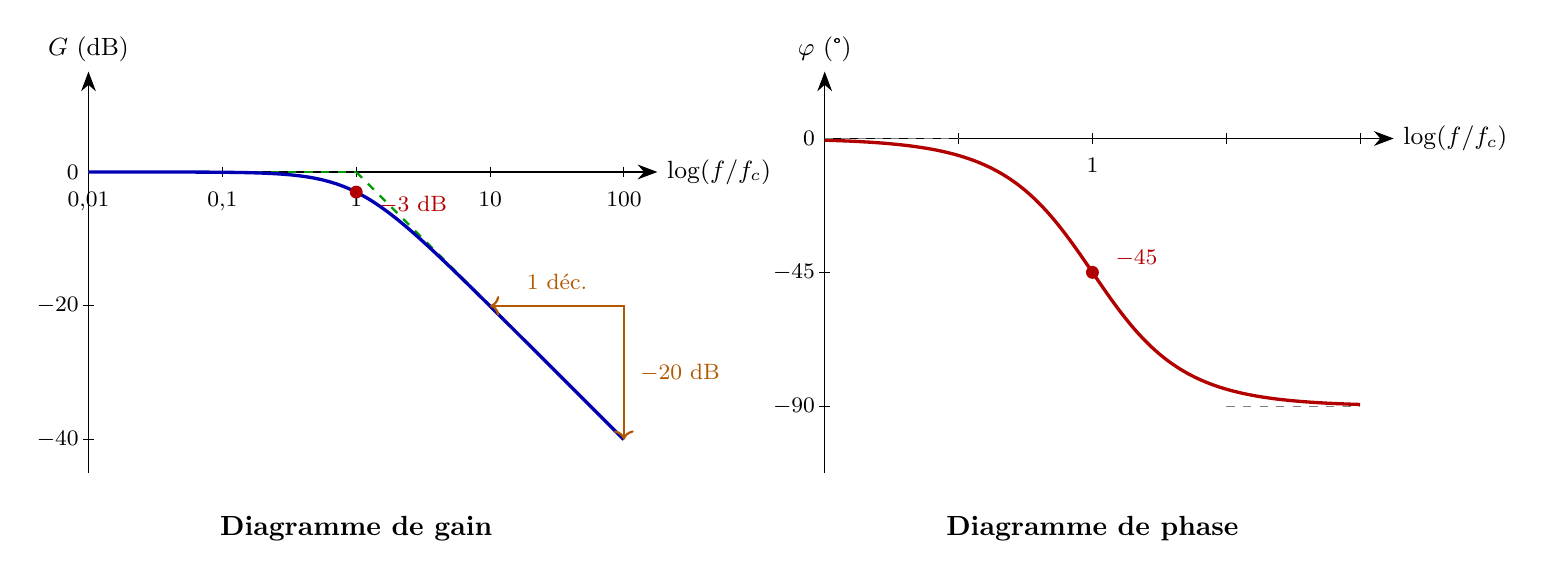
\begin{tikzpicture}[scale=0.85]
  % === GAIN ===
  \begin{scope}[shift={(0,0)}]
    \draw[-{Stealth[length=2.5mm]}] (0,0) -- (8.5,0) node[right, font=\small]{$\log(f/f_c)$};
    \draw[-{Stealth[length=2.5mm]}] (0,-4.5) -- (0,1.5) node[above, font=\small]{$G$ (dB)};
    
    % Graduations
    \foreach \x/\lab in {0/{0.01}, 2/{0.1}, 4/{1}, 6/{10}, 8/{100}} {
      \draw (\x,0.08) -- (\x,-0.08);
    }
    \node[below, font=\footnotesize] at (0,-0.15) {$0{,}01$};
    \node[below, font=\footnotesize] at (2,-0.15) {$0{,}1$};
    \node[below, font=\footnotesize] at (4,-0.15) {$1$};
    \node[below, font=\footnotesize] at (6,-0.15) {$10$};
    \node[below, font=\footnotesize] at (8,-0.15) {$100$};
    
    \node[left, font=\footnotesize] at (0,0) {$0$};
    \node[left, font=\footnotesize] at (0,-2) {$-20$};
    \node[left, font=\footnotesize] at (0,-4) {$-40$};
    \draw (-0.08,-2) -- (0.08,-2);
    \draw (-0.08,-4) -- (0.08,-4);
    
    % Asymptote BF (0 dB)
    \draw[dashed, green!60!black, thick] (0,0) -- (4,0);
    % Asymptote HF (-20 dB/dec)
    \draw[dashed, green!60!black, thick] (4,0) -- (8,-4);
    
    % Courbe réelle : G_dB/10 = -log10(1 + (f/fc)^2), avec (f/fc)^2 = 10^(x-4)
    \draw[very thick, blue!70!black, domain=0:8, samples=200, smooth]
      plot(\x, {-ln(1 + pow(10, \x-4)) / ln(10) });
    
    % Point -3 dB
    \filldraw[red!70!black] (4,-0.3) circle (2.5pt);
    \node[red!70!black, right, font=\footnotesize] at (4.2,-0.5) {$-3$ dB};
    
    % Pente
    \draw[<->, thick, orange!70!black] (6,-2) -- (8,-2) -- (8,-4);
    \node[orange!70!black, font=\footnotesize, right] at (8.1,-3) {$-20$ dB};
    \node[orange!70!black, font=\footnotesize, above] at (7,-1.9) {1 déc.};
    
    \node[below, font=\bfseries] at (4,-5) {Diagramme de gain};
  \end{scope}
  
  % === PHASE ===
  \begin{scope}[shift={(11,0)}]
    \draw[-{Stealth[length=2.5mm]}] (0,0.5) -- (8.5,0.5) node[right, font=\small]{$\log(f/f_c)$};
    \draw[-{Stealth[length=2.5mm]}] (0,-4.5) -- (0,1.5) node[above, font=\small]{$\varphi$ (°)};
    
    % Graduations
    \foreach \x in {0,2,4,6,8} {
      \draw (\x,0.58) -- (\x,0.42);
    }
    \node[below, font=\footnotesize] at (4,0.35) {$1$};
    
    \node[left, font=\footnotesize] at (0,0.5) {$0°$};
    \node[left, font=\footnotesize] at (0,-1.5) {$-45°$};
    \node[left, font=\footnotesize] at (0,-3.5) {$-90°$};
    \draw (-0.08,-1.5) -- (0.08,-1.5);
    \draw (-0.08,-3.5) -- (0.08,-3.5);
    
    % Courbe de phase : phi = -arctan(f/fc), atan en degrés dans pgfmath
    % Échelle : 0° -> y=0.5, -90° -> y=-3.5, donc 1° = 4/90 unités
    \draw[very thick, red!70!black, domain=0:8, samples=200, smooth]
      plot(\x, {0.5 - (4/90)*atan(pow(10, (\x-4)/2)) });
    
    % Point -45°
    \filldraw[red!70!black] (4,-1.5) circle (2.5pt);
    \node[red!70!black, right, font=\footnotesize] at (4.2,-1.3) {$-45°$};
    
    % Asymptotes
    \draw[dashed, gray] (0,0.5) -- (2,0.5);
    \draw[dashed, gray] (6,-3.5) -- (8,-3.5);
    
    \node[below, font=\bfseries] at (4,-5) {Diagramme de phase};
  \end{scope}
\end{tikzpicture}
\end{center}

\begin{intuition}
\textbf{Comment lire ce diagramme :}
\begin{itemize}[nosep]
\item \textbf{En BF} (à gauche de $f_c$) : le gain est $\SI{0}{dB}$ (le signal passe intégralement) et la phase est $\sim 0°$ (pas de décalage). Le filtre est ``transparent''.
\item \textbf{À $f_c$} : le gain a baissé de \SI{3}{dB} (le signal est atténué à $70{,}7\%$) et la phase est $-45°$. C'est le point de coupure.
\item \textbf{En HF} (à droite de $f_c$) : le gain diminue de \SI{20}{dB} par décade (droite descendante). La phase tend vers $-90°$. Le filtre ``bloque'' de plus en plus.
\end{itemize}
Les \textbf{asymptotes} (lignes vertes en pointillé) sont l'approximation de la courbe réelle (bleue). L'écart maximal est de \SI{3}{dB} au point de coupure. En pratique, on trace d'abord les asymptotes, puis on arrondit au voisinage de $f_c$.
\end{intuition}

\subsection{Le filtre passe-haut du 1er ordre}

Si on prend la sortie aux bornes de $R$ dans un circuit RC série (au lieu de $C$) :
\[
\underline{H}(\omega) = \frac{j\omega/\omega_c}{1 + j\omega/\omega_c}
\]

C'est le \textbf{miroir} du passe-bas :
\begin{itemize}[nosep]
\item En BF : gain $\to 0$ ($+\SI{20}{dB/décade}$ de montée).
\item À $f_c$ : gain $= \SI{-3}{dB}$, phase $= +45°$.
\item En HF : gain $\to \SI{0}{dB}$, phase $\to 0°$.
\end{itemize}

\begin{retenir}
\textbf{L'essentiel sur les fonctions de transfert et Bode :}
\begin{enumerate}[nosep]
\item $\underline{H}(\omega) = V_{\text{out}}/V_{\text{in}}$ : module = gain, argument = phase.
\item $G_{\text{dB}} = 20\log|H|$. Les dB transforment les multiplications en additions.
\item Le diagramme de Bode = gain (dB) et phase (°) en fonction de $\log f$.
\item Passe-bas 1er ordre : \SI{0}{dB} en BF, $-\SI{20}{dB/décade}$ en HF, $-\SI{3}{dB}$ et $-45°$ à $f_c$.
\item On trace d'abord les \textbf{asymptotes}, puis on corrige au voisinage des fréquences de coupure.
\end{enumerate}
\end{retenir}

% ----------------------------------------------------------------------------
\section{Approfondissement}

\begin{approfondissement}
Construction systématique des diagrammes de Bode, systèmes du 2nd ordre, mise en cascade, et classification des filtres. Prérequis : logarithmes, fonctions de transfert du 1er ordre.
\end{approfondissement}

\subsection{Écriture normalisée d'une fonction de transfert}

Toute fonction de transfert d'un système linéaire peut se mettre sous la forme d'un rapport de polynômes en $j\omega$ (ou en $p = j\omega$, ou en $s = \sigma + j\omega$ pour Laplace) :

\begin{formule}
\[
\underline{H}(j\omega) = H_0 \cdot \frac{(1 + j\omega/\omega_{z1})(1 + j\omega/\omega_{z2})\cdots}{(1 + j\omega/\omega_{p1})(1 + j\omega/\omega_{p2})\cdots}
\]
\begin{itemize}[nosep]
\item $H_0$ : gain statique (gain en DC, $\omega = 0$).
\item $\omega_{z1}, \omega_{z2}, \ldots$ : \textbf{zéros} (fréquences où le numérateur s'annule $\Rightarrow$ $|H| \to 0$).
\item $\omega_{p1}, \omega_{p2}, \ldots$ : \textbf{pôles} (fréquences où le dénominateur s'annule $\Rightarrow$ $|H| \to \infty$).
\end{itemize}
\end{formule}

\begin{intuition}
\textbf{Pôles et zéros sont les ``ingrédients'' du diagramme de Bode.} Chaque pôle ajoute une cassure vers le bas ($-\SI{20}{dB/décade}$) et $-90°$ de déphasage. Chaque zéro ajoute une cassure vers le haut ($+\SI{20}{dB/décade}$) et $+90°$. Le diagramme de Bode complet est la \textbf{somme} de toutes ces contributions (grâce aux propriétés du logarithme).
\end{intuition}

\subsection{Règles de construction du diagramme de Bode}

\textbf{Étape 1 --- Identifier les éléments :}
\begin{itemize}[nosep]
\item Gain statique $H_0$ $\Rightarrow$ ligne horizontale à $20\log|H_0|$ dB.
\item Chaque pôle à $\omega_{pk}$ $\Rightarrow$ cassure de $-\SI{20}{dB/décade}$ à $f_{pk}$.
\item Chaque zéro à $\omega_{zk}$ $\Rightarrow$ cassure de $+\SI{20}{dB/décade}$ à $f_{zk}$.
\item Éventuel intégrateur ($1/j\omega$) $\Rightarrow$ pente de $-\SI{20}{dB/décade}$ dès $f = 0$.
\item Éventuel dérivateur ($j\omega$) $\Rightarrow$ pente de $+\SI{20}{dB/décade}$ dès $f = 0$.
\end{itemize}

\textbf{Étape 2 --- Tracer le gain asymptotique :}
\begin{itemize}[nosep]
\item Commencer à gauche par le gain BF.
\item À chaque fréquence de pôle/zéro, ajouter/retrancher la pente.
\item La courbe asymptotique est une succession de segments de droite.
\end{itemize}

\textbf{Étape 3 --- Corriger au voisinage des coupures :}
\begin{itemize}[nosep]
\item À chaque pôle/zéro, la courbe réelle s'écarte de l'asymptote de $\SI{3}{dB}$ \textit{exactement à la fréquence de coupure}.
\item L'erreur est de $\SI{1}{dB}$ à $f/2$ et $2f$ (une octave avant/après).
\end{itemize}

\textbf{Étape 4 --- Phase :}
\begin{itemize}[nosep]
\item Chaque pôle contribue $-90°$ (transition sur $\sim 2$ décades, centrée sur la fréquence du pôle).
\item Chaque zéro contribue $+90°$.
\item La phase totale est la somme des contributions.
\end{itemize}

\subsection{Exemple : filtre avec un zéro et un pôle}

Soit $H(j\omega) = 10 \cdot \dfrac{1 + j\omega/\omega_{z}}{1 + j\omega/\omega_{p}}$ avec $f_z = \SI{100}{Hz}$ et $f_p = \SI{10}{kHz}$.

\textbf{Construction :}
\begin{itemize}[nosep]
\item En BF ($f \ll f_z$) : $|H| = 10$ soit $\SI{+20}{dB}$.
\item À $f_z = \SI{100}{Hz}$ : le zéro ajoute $+\SI{20}{dB/décade}$.
\item Entre $f_z$ et $f_p$ : la pente est $+\SI{20}{dB/décade}$. À $f_p$ : $|H| = 10 \times f_p/f_z = 10 \times 100 = 1000$ soit $\SI{+60}{dB}$.
\item À $f_p = \SI{10}{kHz}$ : le pôle ajoute $-\SI{20}{dB/décade}$. Les deux pentes se compensent : le gain redevient plat à $\SI{+60}{dB}$.
\item En HF ($f \gg f_p$) : $|H| \to 10 \times \omega_p/\omega_z = 10 \times 100 = 1000$ soit $\SI{+60}{dB}$ constant.
\end{itemize}

C'est un \textbf{filtre passe-haut étagé} (ou ``lead compensator'') : gain faible en BF, gain élevé en HF, transition entre $f_z$ et $f_p$.

\subsection{Le 2nd ordre : pôles complexes et résonance}

Quand un circuit contient un $L$ et un $C$ (circuit RLC), la fonction de transfert est du \textbf{2nd ordre}. La forme canonique est :

\begin{formule}
\[
\boxed{H(j\omega) = \frac{H_0}{1 + \frac{j\omega}{Q\omega_0} + \left(\frac{j\omega}{\omega_0}\right)^2}} \qquad \text{(passe-bas du 2nd ordre)}
\]
Deux paramètres fondamentaux : $\omega_0$ (pulsation propre) et $Q$ (facteur de qualité).
\end{formule}

\textbf{Comportement sur le diagramme de Bode :}
\begin{itemize}[nosep]
\item En BF : $|H| = H_0$ ($\SI{0}{dB}$ si $H_0 = 1$).
\item En HF : pente de $-\SI{40}{dB/décade}$ (deux pôles = deux fois $-\SI{20}{dB}$).
\item À $\omega_0$ : le comportement dépend de $Q$ :
\end{itemize}

\begin{center}
\renewcommand{\arraystretch}{1.4}
\begin{tabular}{lll}
\toprule
\textbf{$Q$} & \textbf{Gain à $\omega_0$} & \textbf{Allure} \\
\midrule
$Q < 1/\sqrt{2} \approx 0{,}707$ & $< \SI{0}{dB}$ & Pas de bosse, arrondi progressif \\
$Q = 1/\sqrt{2}$ (Butterworth) & $\SI{0}{dB}$ exactement & Plat au maximum, puis $-\SI{40}{dB/déc}$ \\
$Q = 1$ & $\SI{0}{dB}$ (+ léger pic) & Petit pic de résonance \\
$Q = 5$ & $\SI{+14}{dB}$ & Pic marqué de résonance \\
$Q = 50$ & $\SI{+34}{dB}$ & Pic très pointu (filtre sélectif) \\
\bottomrule
\end{tabular}
\end{center}

Le gain au pic de résonance vaut exactement $Q$ en linéaire, soit $20\log Q$ en dB.

\begin{attention}
\textbf{Piège de l'asymptotique au 2nd ordre :} l'asymptote prédit une cassure nette de $-\SI{40}{dB/décade}$ à $\omega_0$. Mais si $Q > 1/\sqrt{2}$, la courbe réelle \textbf{dépasse} l'asymptote avant de la rejoindre : c'est le pic de résonance. L'écart peut être considérable ($\SI{34}{dB}$ pour $Q = 50$). \textbf{Ne jamais se fier à l'asymptotique seul au 2nd ordre} quand $Q$ est élevé.
\end{attention}

\begin{pratique}
\textbf{Filtres classiques du 2nd ordre selon $Q$ :}
\begin{itemize}[nosep]
\item $Q = 0{,}707$ (Butterworth) : \textbf{réponse la plus plate possible} dans la bande passante. Pas de bosse, pas d'ondulation. C'est le filtre ``passe-partout''.
\item $Q = 0{,}577$ (Bessel) : \textbf{phase la plus linéaire possible} (retard de groupe constant). Préserve la forme des impulsions. Utilisé en transmission de données.
\item $Q > 0{,}707$ (Tchebychev, elliptique) : ondulation dans la bande passante, mais \textbf{transition plus raide} vers la bande coupée. Utilisé quand on veut une forte réjection proche de $f_c$.
\end{itemize}
\end{pratique}

\subsection{Systèmes en cascade}

Quand plusieurs étages sont en cascade (sortie du premier = entrée du second), la fonction de transfert totale est le \textbf{produit} des fonctions de transfert individuelles :

\begin{formule}
\[
\underline{H}_{\text{total}} = \underline{H}_1 \times \underline{H}_2 \times \cdots
\]
En décibels (grâce au logarithme) :
\[
\boxed{G_{\text{total, dB}} = G_{1,\text{dB}} + G_{2,\text{dB}} + \cdots}
\]
\[
\boxed{\varphi_{\text{total}} = \varphi_1 + \varphi_2 + \cdots}
\]
Les gains en dB \textbf{s'additionnent}. Les phases aussi.
\end{formule}

\begin{attention}
Cette propriété n'est valable que si chaque étage \textbf{ne charge pas le précédent} (impédance d'entrée $\gg$ impédance de sortie de l'étage précédent). Sinon, la fonction de transfert totale n'est pas le simple produit. En pratique, on intercale des \textbf{buffers} (suiveurs) entre les étages pour garantir l'indépendance.
\end{attention}

\subsection{Classification des filtres}

\begin{center}
\renewcommand{\arraystretch}{1.5}
\begin{tabular}{lp{5cm}p{5cm}}
\toprule
\textbf{Type} & \textbf{Ce qui passe} & \textbf{Exemple d'usage} \\
\midrule
\textbf{Passe-bas} (LP) & BF, atténue HF & Anti-aliasing (ADC), lissage, filtrage bruit \\
\textbf{Passe-haut} (HP) & HF, atténue BF & Couplage AC (supprime le DC), micro \\
\textbf{Passe-bande} (BP) & Bande autour de $f_0$ & Récepteur radio, sélection de canal \\
\textbf{Coupe-bande} (BS/Notch) & Tout sauf $f_0$ & Suppression \SI{50}{Hz}, filtre anti-larsen \\
\textbf{Passe-tout} & Tout (gain = 1) mais modifie la phase & Égalisation de phase, déphaseur \\
\bottomrule
\end{tabular}
\end{center}

\begin{intuition}
Tout filtre peut se construire à partir de combinaisons de passe-bas et passe-haut :
\begin{itemize}[nosep]
\item Passe-bande = passe-haut $\times$ passe-bas (intersection des deux bandes).
\item Coupe-bande = passe-bas $+$ passe-haut (union des deux bandes).
\end{itemize}
\end{intuition}

\subsection{Fonction de transfert en variable de Laplace $s$ (aperçu)}

Pour les systèmes asservis et l'analyse de stabilité, on utilise la \textbf{variable de Laplace} $s = \sigma + j\omega$ au lieu de $j\omega$ seul :

\begin{formule}
\[
H(s) = \frac{N(s)}{D(s)} = \frac{b_m s^m + \cdots + b_1 s + b_0}{a_n s^n + \cdots + a_1 s + a_0}
\]
\begin{itemize}[nosep]
\item Les racines de $N(s) = 0$ sont les \textbf{zéros}.
\item Les racines de $D(s) = 0$ sont les \textbf{pôles}.
\item Pour le régime sinusoïdal permanent : on pose $s = j\omega$.
\item L'avantage de $s$ : il permet aussi d'étudier la \textbf{stabilité} (pôles dans le plan complexe).
\end{itemize}
\end{formule}

\begin{intuition}
$j\omega$ est un cas particulier de $s$ : c'est la restriction à l'axe imaginaire du plan complexe. $H(j\omega)$ donne la réponse fréquentielle. $H(s)$ donne en plus le comportement transitoire et la stabilité. C'est l'outil central de l'automatique et de la conception des boucles de rétroaction.

La section Niveau Ingénieur développera la stabilité, les critères de Routh-Hurwitz et de Nyquist, et les marges de phase et de gain.
\end{intuition}


% ----------------------------------------------------------------------------
\section{Niveau Ingénieur}

\begin{ingenieur}
Stabilité des systèmes bouclés, critères de Routh-Hurwitz et de Nyquist, marges de gain et de phase. Ce sont les outils fondamentaux de la conception des amplificateurs à rétroaction, des alimentations régulées et des boucles d'asservissement.
\end{ingenieur}

\subsection{Boucle ouverte et boucle fermée}

La plupart des systèmes électroniques réels utilisent une \textbf{rétroaction} (feedback) : une partie du signal de sortie est renvoyée à l'entrée pour contrôler le comportement. C'est le cas des amplificateurs opérationnels bouclés, des régulateurs de tension, des PLL, des asservissements de moteur\ldots

\begin{center}
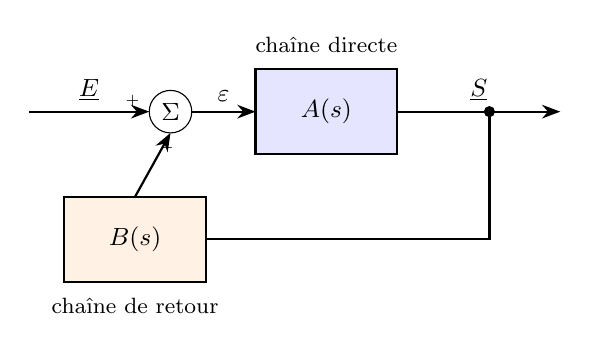
\begin{tikzpicture}[scale=0.9, >=Stealth, every node/.style={font=\small}]
  % Comparateur
  \draw (0,0) circle (0.3);
  \node at (0,0) {$\Sigma$};
  \node[left] at (-0.3,0.15) {\tiny $+$};
  \node[below] at (-0.05,-0.3) {\tiny $-$};
  
  % Entrée
  \draw[->, thick] (-2,0) -- (-0.3,0) node[midway, above]{$\underline{E}$};
  
  % Bloc A(s)
  \draw[thick, fill=blue!10] (1.2,-0.6) rectangle (3.2,0.6);
  \node at (2.2,0) {$A(s)$};
  \draw[->, thick] (0.3,0) -- (1.2,0) node[midway, above]{$\varepsilon$};
  
  % Sortie
  \draw[->, thick] (3.2,0) -- (5.5,0) node[midway, above]{$\underline{S}$};
  
  % Point de prélèvement
  \filldraw (4.5,0) circle (2pt);
  
  % Retour
  \draw[thick] (4.5,0) -- (4.5,-1.8) -- (-1.5,-1.8);
  
  % Bloc B(s)
  \draw[thick, fill=orange!10] (-1.5,-2.4) rectangle (0.5,-1.2);
  \node at (-0.5,-1.8) {$B(s)$};
  
  \draw[->, thick] (-0.5,-1.2) -- (0,-0.3);
  
  % Labels
  \node[above, font=\footnotesize] at (2.2,0.7) {chaîne directe};
  \node[below, font=\footnotesize] at (-0.5,-2.5) {chaîne de retour};
\end{tikzpicture}
\end{center}

\begin{formule}
\textbf{Fonction de transfert en boucle ouverte} (FTBO) :
\[
T(s) = A(s) \cdot B(s)
\]

\textbf{Fonction de transfert en boucle fermée} (FTBF) :
\[
\boxed{H_{\text{BF}}(s) = \frac{A(s)}{1 + A(s)\cdot B(s)} = \frac{A(s)}{1 + T(s)}}
\]

Si le gain de boucle $|T| \gg 1$ : $H_{\text{BF}} \approx 1/B(s)$ (la sortie ne dépend plus que du retour). C'est le principe fondamental de la rétroaction négative.
\end{formule}

\begin{intuition}
\textbf{Pourquoi la rétroaction ?} Elle permet de rendre le comportement \textbf{insensible} aux variations de la chaîne directe (température, vieillissement, dispersion des composants). Un ampli-op avec un gain en boucle ouverte de 100\,000 (qui varie de $\pm 50\%$) donne, une fois bouclé avec $B = 1/10$, un gain de $\sim 10$ stable à $\pm 0{,}01\%$.

\textbf{Le prix à payer :} la rétroaction peut rendre le système \textbf{instable} si la boucle introduit trop de déphasage. C'est tout l'enjeu de l'analyse de stabilité.
\end{intuition}

\subsection{Condition d'instabilité}

Le dénominateur de $H_{\text{BF}}$ est $1 + T(s)$. Si $T(s) = -1$ (c'est-à-dire $|T| = 1$ et $\arg(T) = -180°$), le dénominateur s'annule et le gain en boucle fermée \textbf{diverge} : le système \textbf{oscille}.

\begin{formule}
\textbf{Condition d'oscillation (critère de Barkhausen) :}
\[
\boxed{|T(j\omega)| = 1 \quad \text{et} \quad \arg(T(j\omega)) = -180°}
\]
Si ces deux conditions sont remplies simultanément à une fréquence $\omega$, le système est instable à cette fréquence (il oscille).
\end{formule}

\begin{attention}
C'est la même condition qui fait fonctionner les \textbf{oscillateurs} (on la cherche volontairement) et qui fait \textbf{planter} les amplificateurs (on l'évite à tout prix). La différence est dans l'intention du concepteur.
\end{attention}

\subsection{Marges de gain et de phase}

Pour qu'un système bouclé soit stable avec une marge de sécurité, on définit deux grandeurs lues directement sur le \textbf{diagramme de Bode de la FTBO} $T(j\omega)$ :

\begin{formule}
\textbf{Marge de phase} ($M_\varphi$) : déphasage restant avant $-180°$ à la fréquence où $|T| = \SI{0}{dB}$ (gain unité).
\[
\boxed{M_\varphi = 180° + \arg(T(j\omega_0))} \qquad \text{où } |T(j\omega_0)| = 1
\]

\textbf{Marge de gain} ($M_G$) : atténuation restante avant $\SI{0}{dB}$ à la fréquence où $\arg(T) = -180°$.
\[
\boxed{M_G = -|T(j\omega_{180})|_{\text{dB}}} \qquad \text{où } \arg(T(j\omega_{180})) = -180°
\]
\end{formule}

\begin{center}
\begin{tikzpicture}[scale=0.8, >=Stealth]
  % === GAIN ===
  \begin{scope}[shift={(0,0)}]
    \draw[->] (0,0) -- (8,0) node[right, font=\small]{$\log f$};
    \draw[->] (0,-3.5) -- (0,3) node[above, font=\small]{$|T|$ (dB)};
    
    \node[left, font=\footnotesize] at (0,0) {$0$};
    \draw[dashed, gray] (0,0) -- (7.5,0);
    
    % Courbe de gain BO
    \draw[very thick, blue!70!black] (0.5,2.5) -- (2,2.5) -- (5,-1) -- (7.5,-3);
    
    % f0 dB et f_180
    \draw[dashed, red!70!black] (3.86,0) -- (3.86,-3.5);
    \node[below, red!70!black, font=\footnotesize] at (3.86,-3.5) {$f_{0\text{dB}}$};
    
    \draw[dashed, orange!70!black] (6.2,0) -- (6.2,-2.2);
    \node[below, orange!70!black, font=\footnotesize] at (6.2,-3.5) {$f_{-180°}$};
    \filldraw[orange!70!black] (6.2,-2.2) circle (2pt);
    
    % Marge de gain
    \draw[<->, very thick, orange!70!black] (6.5,0) -- (6.5,-2.2);
    \node[orange!70!black, font=\footnotesize, right] at (6.6,-1.1) {$M_G$};
    
    \node[font=\bfseries\small] at (4,-4.5) {Gain};
  \end{scope}
  
  % === PHASE ===
  \begin{scope}[shift={(10,0)}]
    \draw[->] (0,0.5) -- (8,0.5) node[right, font=\small]{$\log f$};
    \draw[->] (0,-3.5) -- (0,1.5) node[above, font=\small]{$\arg(T)$};
    
    \node[left, font=\footnotesize] at (0,0.5) {$0°$};
    \node[left, font=\footnotesize] at (0,-1) {$-90°$};
    \node[left, font=\footnotesize] at (0,-2.5) {$-180°$};
    \draw[dashed, gray] (0,-2.5) -- (7.5,-2.5);
    
    % Courbe de phase BO
    \draw[very thick, red!70!black] (0.5,0.3) -- (1.5,0) -- (3,-1) -- (5,-2.3) -- (7.5,-3.2);
    
    % f0 dB
    \draw[dashed, red!70!black] (3.86,0.5) -- (3.86,-2.5);
    \node[above, red!70!black, font=\footnotesize] at (3.86,0.6) {$f_{0\text{dB}}$};
    \filldraw[red!70!black] (3.86,-1.7) circle (2pt);
    
    % Marge de phase
    \draw[<->, very thick, red!70!black] (4.16,-1.7) -- (4.16,-2.5);
    \node[red!70!black, font=\footnotesize, right] at (4.26,-2.1) {$M_\varphi$};
    
    % f_180
    \draw[dashed, orange!70!black] (6.2,0.5) -- (6.2,-2.5);
    \node[above, orange!70!black, font=\footnotesize] at (6.2,0.6) {$f_{-180°}$};
    
    \node[font=\bfseries\small] at (4,-4.5) {Phase};
  \end{scope}
\end{tikzpicture}
\end{center}

\begin{pratique}
\textbf{Valeurs cibles en conception :}
\begin{center}
\begin{tabular}{ll}
\toprule
\textbf{Critère} & \textbf{Valeur typique} \\
\midrule
Marge de phase & $> 45°$ (idéal : $60°$--$70°$) \\
Marge de gain & $> \SI{6}{dB}$ (idéal : \SI{10}{dB}--\SI{12}{dB}) \\
\bottomrule
\end{tabular}
\end{center}

\begin{itemize}[nosep]
\item $M_\varphi < 45°$ : réponse transitoire oscillante (dépassement important).
\item $M_\varphi < 0°$ : \textbf{instable} (le système oscille).
\item $M_\varphi \approx 60°$ : bon compromis rapidité/stabilité (correspond à $Q \approx 0{,}7$ en boucle fermée).
\end{itemize}
\end{pratique}

\subsection{Critère de Routh-Hurwitz}

Le critère de Routh-Hurwitz est une méthode \textbf{algébrique} pour déterminer si un polynôme a toutes ses racines à partie réelle négative (c'est-à-dire si le système est stable) \textit{sans calculer les racines}.

Soit le dénominateur de $H_{\text{BF}}$ :
\[
D(s) = a_n s^n + a_{n-1} s^{n-1} + \cdots + a_1 s + a_0
\]

\begin{formule}
\textbf{Condition nécessaire :} tous les coefficients $a_k$ doivent être de \textbf{même signe} et \textbf{non nuls}. Si un coefficient est nul ou de signe opposé, le système est instable (ou à la limite de stabilité).

\textbf{Condition nécessaire et suffisante :} construire le \textbf{tableau de Routh} et vérifier que tous les éléments de la première colonne sont de même signe.
\end{formule}

\textbf{Construction du tableau de Routh :}

\begin{center}
\renewcommand{\arraystretch}{1.4}
\begin{tabular}{c|cccc}
$s^n$ & $a_n$ & $a_{n-2}$ & $a_{n-4}$ & $\cdots$ \\
$s^{n-1}$ & $a_{n-1}$ & $a_{n-3}$ & $a_{n-5}$ & $\cdots$ \\
$s^{n-2}$ & $b_1$ & $b_2$ & $b_3$ & $\cdots$ \\
$s^{n-3}$ & $c_1$ & $c_2$ & $\cdots$ & \\
$\vdots$ & $\vdots$ & & & \\
$s^0$ & $\cdots$ & & & \\
\end{tabular}
\end{center}

avec $b_1 = \dfrac{a_{n-1}\cdot a_{n-2} - a_n\cdot a_{n-3}}{a_{n-1}}$, \quad $b_2 = \dfrac{a_{n-1}\cdot a_{n-4} - a_n\cdot a_{n-5}}{a_{n-1}}$, \quad etc.

Chaque ligne se calcule à partir des deux lignes précédentes par la même formule de ``déterminant croisé'' divisé par le premier élément de la ligne du dessus.

\begin{formule}
\textbf{Critère :} le nombre de changements de signe dans la \textbf{première colonne} du tableau est égal au nombre de racines à partie réelle positive (pôles instables).
\begin{itemize}[nosep]
\item Aucun changement de signe $\Rightarrow$ \textbf{stable}.
\item $k$ changements de signe $\Rightarrow$ $k$ pôles instables.
\end{itemize}
\end{formule}

\textbf{Exemple :} $D(s) = s^3 + 6s^2 + 11s + 6$.

\begin{center}
\begin{tabular}{c|cc}
$s^3$ & $1$ & $11$ \\
$s^2$ & $6$ & $6$ \\
$s^1$ & $(6\times11 - 1\times6)/6 = 10$ & \\
$s^0$ & $(10\times6 - 6\times0)/10 = 6$ & \\
\end{tabular}
\end{center}

Première colonne : $1, 6, 10, 6$ --- tous positifs. \textbf{Aucun changement de signe} $\Rightarrow$ système stable. (On peut vérifier : $s^3+6s^2+11s+6 = (s+1)(s+2)(s+3)$, trois pôles réels négatifs.)

\textbf{Contre-exemple :} $D(s) = s^3 + 2s^2 + s + 8$.

\begin{center}
\begin{tabular}{c|cc}
$s^3$ & $1$ & $1$ \\
$s^2$ & $2$ & $8$ \\
$s^1$ & $(2\times1 - 1\times8)/2 = -3$ & \\
$s^0$ & $(-3\times8 - 2\times0)/(-3) = 8$ & \\
\end{tabular}
\end{center}

Première colonne : $1, 2, \mathbf{-3}, 8$ --- deux changements de signe ($+\to-$ et $-\to+$). Donc \textbf{2 pôles instables} (à partie réelle positive). Le système est instable.

\subsection{Critère de Nyquist (présentation qualitative)}

Le critère de Nyquist examine la FTBO $T(j\omega)$ dans le \textbf{plan complexe} (diagramme de Nyquist) : on trace $T(j\omega)$ pour $\omega$ allant de $0$ à $\infty$.

\begin{formule}
\textbf{Version simplifiée} (système stable en boucle ouverte) : le système en boucle fermée est \textbf{stable} si et seulement si le point critique $(-1, 0)$ est \textbf{à gauche} de la courbe de Nyquist quand on la parcourt dans le sens des $\omega$ croissants. Autrement dit, la courbe ne doit pas ``entourer'' le point $-1$.
\end{formule}

\begin{intuition}
Le critère de Nyquist est \textbf{plus général} que Routh-Hurwitz car il fonctionne aussi pour les systèmes à retard pur (fréquents en numérique et en processus industriels). En pratique, pour les circuits électroniques analogiques, les marges de gain et de phase (lues sur le Bode) sont plus faciles à utiliser et suffisent dans la grande majorité des cas.
\end{intuition}

\subsection{Compensation et stabilisation}

Quand un système bouclé a une marge de phase insuffisante, on ajoute un réseau de \textbf{compensation} pour modifier le Bode de la FTBO.

\begin{pratique}
\textbf{Techniques courantes :}
\begin{itemize}[nosep]
\item \textbf{Compensation dominante (pôle dominant)} : on ajoute un pôle à basse fréquence qui force le gain à croiser \SI{0}{dB} bien avant que la phase n'atteigne $-180°$. C'est ce que fait la capacité de compensation ``Miller'' dans un ampli-op (typiquement $\SI{30}{pF}$ interne).
\item \textbf{Avance de phase (lead)} : un réseau zéro-pôle ($f_z < f_p$) qui ``remonte'' la phase au voisinage du croisement à \SI{0}{dB}. Utilisé dans les régulateurs de tension et les boucles PLL.
\item \textbf{Retard de phase (lag)} : un réseau pôle-zéro ($f_p < f_z$) qui augmente le gain en BF (réduit l'erreur statique) sans affecter la phase au croisement. Utilisé en automatique.
\item \textbf{PID} : combinaison d'un intégrateur (erreur statique nulle), d'un proportionnel (gain) et d'un dérivateur (avance de phase). C'est le correcteur universel des systèmes asservis. Il sera détaillé dans un chapitre dédié.
\end{itemize}
\end{pratique}

\subsection{Lien avec la simulation SPICE}

\begin{pratique}
En simulation, le diagramme de Bode s'obtient par une \textbf{analyse .AC} :

\begin{verbatim}
.ac dec 100 1 100Meg
\end{verbatim}

Cette commande balaye la fréquence de \SI{1}{Hz} à \SI{100}{MHz} avec 100 points par décade. SPICE calcule $\underline{V}_{\text{out}}/\underline{V}_{\text{in}}$ à chaque fréquence et affiche le gain (dB) et la phase (°).

\textbf{Pour l'analyse de stabilité d'une boucle :} on ``coupe'' la boucle en un point, on injecte un signal de test, et on mesure la FTBO. Les marges se lisent directement sur le Bode résultant. Des outils comme LTspice, ngspice ou QSPICE le font nativement.
\end{pratique}

% === EXERCICES DU CHAPITRE 13 ===
\section*{Exercices}
\addcontentsline{toc}{section}{Exercices}

\subsection*{Niveau débutant}

\textbf{Exercice 13.1 ---} Convertissez les gains suivants en dB : $|H| = 0{,}5$ ; $|H| = 20$ ; $|H| = 300$.

\begin{pratique}
\textbf{Solution :}

$0{,}5 = 1/2 \Rightarrow \SI{-6}{dB}$.

$20 = 2\times10 \Rightarrow 6 + 20 = \SI{+26}{dB}$.

$300 = 3\times100 \Rightarrow 10 + 40 = \SI{+50}{dB}$ (approximation ; exact : $20\log 300 = \SI{49.5}{dB}$).
\end{pratique}

\textbf{Exercice 13.2 ---} Un filtre passe-bas du 1er ordre a $f_c = \SI{10}{kHz}$. Quel est le gain en dB à \SI{100}{kHz} ? À \SI{1}{MHz} ? Quel est le déphasage à $f_c$ ?

\begin{pratique}
\textbf{Solution :} Au-delà de $f_c$, l'atténuation est de $-\SI{20}{dB/décade}$.

À \SI{100}{kHz} ($= 10\times f_c$, 1 décade) : $G \approx 0 - 20 = \SI{-20}{dB}$.

À \SI{1}{MHz} ($= 100\times f_c$, 2 décades) : $G \approx 0 - 40 = \SI{-40}{dB}$.

Déphasage à $f_c$ : $\varphi = -45°$.
\end{pratique}

\subsection*{Niveau intermédiaire}

\textbf{Exercice 13.3 ---} Un circuit comporte $R_1 = \SI{10}{k\ohm}$ en série avec le parallèle de $R_2 = \SI{10}{k\ohm}$ et $C = \SI{10}{nF}$ (sortie aux bornes de $R_2 \parallel C$). Trouvez $H(j\omega)$, identifiez le type de filtre, calculez $f_c$ et le gain statique. Tracez le diagramme de Bode asymptotique.

\begin{pratique}
\textbf{Solution :} $\underline{Z}_2 = R_2 \parallel (1/j\omega C) = \dfrac{R_2}{1 + j\omega R_2 C}$.

$\underline{H} = \dfrac{\underline{Z}_2}{R_1 + \underline{Z}_2} = \dfrac{R_2}{R_1(1+j\omega R_2 C) + R_2} = \dfrac{R_2}{R_1 + R_2 + j\omega R_1 R_2 C}$

$= \dfrac{R_2/(R_1+R_2)}{1 + j\omega \cdot R_1 R_2 C/(R_1+R_2)}$

Gain statique : $H_0 = R_2/(R_1+R_2) = 10/20 = 0{,}5$ soit $\SI{-6}{dB}$.

Fréquence de coupure : $\omega_c = (R_1+R_2)/(R_1 R_2 C) = 20000/(10^4\times10^4\times10^{-8}) = 20000/10^{-4+8} = \SI{2e4}{} \Rightarrow f_c = \omega_c/(2\pi) \approx \SI{3.18}{kHz}$.

C'est un \textbf{filtre passe-bas du 1er ordre} avec gain statique de $\SI{-6}{dB}$, coupure à $\SI{3.18}{kHz}$, pente $-\SI{20}{dB/décade}$ en HF.

Bode asymptotique : horizontale à $\SI{-6}{dB}$ jusqu'à $\SI{3.18}{kHz}$, puis descente à $-\SI{20}{dB/déc}$.
\end{pratique}

\textbf{Exercice 13.4 ---} Deux étages identiques de filtre passe-bas ($f_c = \SI{1}{kHz}$, gain $\SI{0}{dB}$) sont mis en cascade (avec un buffer entre les deux pour éviter le chargement). Quel est le gain total à \SI{1}{kHz} ? À \SI{10}{kHz} ? Quelle est la pente asymptotique HF ?

\begin{pratique}
\textbf{Solution :} En cascade, les gains en dB s'additionnent.

Chaque étage à \SI{1}{kHz} : $\SI{-3}{dB}$. Total : $-3-3 = \SI{-6}{dB}$.

Chaque étage à \SI{10}{kHz} (1 décade au-dessus) : $\approx\SI{-20}{dB}$. Total : $-20-20 = \SI{-40}{dB}$.

Pente HF : $-20 - 20 = -\SI{40}{dB/décade}$. C'est l'équivalent d'un filtre du 2nd ordre.

\textbf{Attention :} la fréquence de coupure à $\SI{-3}{dB}$ du système total n'est \textit{pas} \SI{1}{kHz}. Il faut trouver $f$ tel que $|H_{\text{tot}}|^2 = 1/2$, soit $[1+(f/f_c)^2]^2 = 2$, d'où $f_{c,\text{tot}} = f_c\sqrt{\sqrt{2}-1} \approx 0{,}644\times f_c = \SI{644}{Hz}$. La bande passante a \textbf{rétréci}.
\end{pratique}

\subsection*{Niveau ingénieur}

\textbf{Exercice 13.5 ---} Un amplificateur opérationnel a un gain en boucle ouverte $A(s) = \dfrac{10^5}{(1+s/\omega_1)(1+s/\omega_2)}$ avec $f_1 = \SI{10}{Hz}$ et $f_2 = \SI{1}{MHz}$. Il est bouclé avec $B = 0{,}1$ (gain visé en BF : $1/B = 10$).

(a) Calculez le gain de boucle $T = AB$ en BF et le produit gain-bande.

(b) À quelle fréquence $|T| = \SI{0}{dB}$ ? Combien de pôles contribuent à la phase à ce point ? Estimez la marge de phase.

(c) Le système est-il stable ? Si non, proposez une compensation.

\begin{pratique}
\textbf{Solution :}

(a) $T_0 = A_0 \times B = 10^5 \times 0{,}1 = 10^4$ soit $\SI{80}{dB}$.

Produit gain-bande : $\text{GBW} = A_0 \times f_1 = 10^5 \times 10 = \SI{1}{MHz}$ (le gain de l'AOP croise \SI{0}{dB} à $\sim\SI{1}{MHz}$).

(b) Le gain de boucle $|T|$ part de $\SI{80}{dB}$ et descend à $-\SI{20}{dB/déc}$ après $f_1 = \SI{10}{Hz}$, puis $-\SI{40}{dB/déc}$ après $f_2 = \SI{1}{MHz}$.

$|T| = \SI{0}{dB}$ : en première approximation, entre $f_1$ et $f_2$ la pente est $-\SI{20}{dB/déc}$. De $\SI{80}{dB}$ à $\SI{10}{Hz}$, il faut 4 décades pour atteindre $\SI{0}{dB}$ : $f_{0\text{dB}} \approx 10 \times 10^4 = \SI{100}{kHz}$.

À \SI{100}{kHz}, le pôle $f_1 = \SI{10}{Hz}$ contribue $\approx -90°$ (on est 4 décades au-dessus). Le pôle $f_2 = \SI{1}{MHz}$ contribue $\approx -\arctan(0{,}1) \approx -6°$.

Phase totale $\approx -90° - 6° = -96°$. Marge de phase $= 180° - 96° = 84°$. \textbf{Stable} avec une bonne marge.

(c) Pas besoin de compensation dans ce cas : la marge est confortable. Le croisement à \SI{0}{dB} se fait à une décade en dessous du 2e pôle, donc avec une pente de $-\SI{20}{dB/déc}$ et une phase $< -135°$. C'est la situation typique d'un AOP compensé internement.

Si $f_2$ était à \SI{100}{kHz} (= $f_{0\text{dB}}$), la phase serait $-90° - 45° = -135°$ et la marge de phase tomberait à $45°$ (limite). Si $f_2 < f_{0\text{dB}}$, on passerait à $-\SI{40}{dB/déc}$ au croisement et $M_\varphi < 45°$ : compensation nécessaire.
\end{pratique}

\textbf{Exercice 13.6 ---} Le polynôme caractéristique d'un système bouclé est $D(s) = s^3 + 4s^2 + 5s + K$ où $K$ est un gain ajustable. Utilisez le critère de Routh-Hurwitz pour trouver la plage de $K$ assurant la stabilité.

\begin{pratique}
\textbf{Solution :} Tableau de Routh :

\begin{center}
\begin{tabular}{c|cc}
$s^3$ & $1$ & $5$ \\
$s^2$ & $4$ & $K$ \\
$s^1$ & $(4\times5 - 1\times K)/4 = (20-K)/4$ & \\
$s^0$ & $K$ & \\
\end{tabular}
\end{center}

Conditions de stabilité (tous les éléments de la 1ère colonne de même signe, ici positifs) :
\begin{itemize}[nosep]
\item $1 > 0$ \checkmark
\item $4 > 0$ \checkmark
\item $(20-K)/4 > 0 \Rightarrow K < 20$
\item $K > 0$
\end{itemize}

\[
\boxed{0 < K < 20}
\]

Pour $K = 20$ : le système est à la \textbf{limite de stabilité} (une ligne de zéros dans le tableau = pôles imaginaires purs = oscillation permanente).

Pour $K > 20$ : instable. Pour $K < 0$ : instable aussi (et physiquement, un gain négatif correspondrait à une rétroaction positive).

\textbf{Interprétation :} plus on augmente le gain $K$ de la boucle, plus on risque l'instabilité. C'est le compromis fondamental de toute conception à rétroaction : \textit{gain élevé = précision mais risque d'instabilité}.
\end{pratique}

\textbf{Exercice 13.7 ---} Un régulateur de tension a une FTBO dont le Bode montre : gain qui croise \SI{0}{dB} à $f = \SI{50}{kHz}$ avec une phase de $-120°$. La phase atteint $-180°$ à $f = \SI{200}{kHz}$ avec un gain de $\SI{-8}{dB}$.

Calculez la marge de phase et la marge de gain. Le système est-il suffisamment stable ? Si la marge de phase est insuffisante, proposez une action corrective et estimez son effet.

\begin{pratique}
\textbf{Solution :}

$M_\varphi = 180° - 120° = 60°$. $M_G = 0 - (-8) = \SI{8}{dB}$.

Les deux marges sont \textbf{correctes} ($M_\varphi > 45°$ et $M_G > \SI{6}{dB}$). Le système est stable avec un bon compromis.

Si $M_\varphi$ était insuffisante (par ex. $30°$) : ajouter un \textbf{réseau d'avance de phase} (lead compensator) centré sur $f_{0\text{dB}}$. Un réseau lead avec un rapport $f_p/f_z = 3$ remonte la phase d'environ $30°$ au maximum. On placerait $f_z \approx \SI{30}{kHz}$ et $f_p \approx \SI{90}{kHz}$ pour maximiser l'avance à \SI{50}{kHz}.
\end{pratique}

\textbf{Exercice 13.8 ---} Un filtre passe-bas du 2nd ordre (Sallen-Key) a $f_0 = \SI{10}{kHz}$ et $Q = 5$. Quel est le pic de gain à la résonance en dB ? Quel est le gain à $f = \SI{100}{kHz}$ ? Pourquoi ce filtre n'est-il pas adapté comme filtre anti-aliasing pour un ADC échantillonnant à \SI{200}{kHz} ?

\begin{pratique}
\textbf{Solution :} Pic de résonance : $G_{\text{pic}} = 20\log Q = 20\log 5 = \SI{14}{dB}$.

Le filtre \textbf{amplifie} les fréquences proches de $f_0$ de \SI{14}{dB}. Cela peut saturer l'ADC.

À $f = \SI{100}{kHz}$ ($= 10f_0$, 1 décade au-dessus) : $G \approx \SI{14}{dB} - \SI{40}{dB} = \SI{-26}{dB}$. (Approximation : le pic est à $f_0$, pente $-\SI{40}{dB/déc}$ après.)

Calcul exact : $|H(10\omega_0)| = 1/\sqrt{(1-100)^2 + (10/5)^2} = 1/\sqrt{9801+4} = 1/99 \approx \SI{-40}{dB}$.

Problème pour l'ADC : $f_s/2 = \SI{100}{kHz}$. À cette fréquence, l'atténuation n'est que de $\SI{-40}{dB}$, ce qui peut être insuffisant pour rejeter le repliement si le signal d'entrée contient des composantes à $\SI{100}{kHz}$.

De plus, le $Q = 5$ crée un pic de $\SI{14}{dB}$ qui peut provoquer de la saturation en amont de l'ADC.

\textbf{Solution :} utiliser un filtre \textbf{Butterworth} ($Q = 0{,}707$, pas de pic) ou un \textbf{Bessel} ($Q = 0{,}577$, phase linéaire), d'ordre supérieur (4 ou 6) pour obtenir une réjection suffisante à $f_s/2$.
\end{pratique}

\subsection*{Questions de compréhension}

\begin{enumerate}[nosep]
\item Pourquoi utilise-t-on une échelle logarithmique en fréquence (et pas linéaire) pour les diagrammes de Bode ?
\item Un amplificateur a un gain en boucle ouverte de \SI{100}{dB} et une bande passante de \SI{10}{Hz}. On le boucle pour obtenir un gain de \SI{20}{dB}. Quelle est la bande passante en boucle fermée (approximation du produit gain-bande constant) ?
\item Expliquez physiquement pourquoi une rétroaction négative peut devenir instable. À quelle fréquence le déphasage transforme-t-il la rétroaction négative en rétroaction positive ?
\item Un système a deux pôles à $f_1$ et $f_2$. Si $f_2 = 2f_1$, la phase au croisement à \SI{0}{dB} est proche de $-180°$. Pourquoi est-ce un cas critique pour la stabilité ? Que se passe-t-il si on ajoute un 3e pôle ?
\end{enumerate}

% === RÉSUMÉ DU CHAPITRE 13 ===
\section*{Résumé du chapitre}
\addcontentsline{toc}{section}{Résumé du chapitre}

\begin{bases}[title={\color{white} Résumé --- Les Bases}]
\begin{center}
\renewcommand{\arraystretch}{1.3}
\begin{tabular}{p{4cm}p{9cm}}
\toprule
Fonction de transfert & $\underline{H} = V_{\text{out}}/V_{\text{in}}$ : module = gain, argument = phase \\
Décibel & $G_{\text{dB}} = 20\log|H|$ ; $-\SI{3}{dB}$ = fréquence de coupure \\
Diagramme de Bode & Gain (dB) et phase (°) vs $\log f$ \\
Passe-bas 1er ordre & $\SI{0}{dB}$ en BF, $-\SI{20}{dB/déc}$ en HF, $-45°$ à $f_c$ \\
Asymptotes & Tracer d'abord les droites, corriger à $\pm\SI{3}{dB}$ aux coupures \\
\bottomrule
\end{tabular}
\end{center}
\end{bases}

\begin{approfondissement}[title={\color{white} Résumé --- Approfondissement}]
\begin{center}
\renewcommand{\arraystretch}{1.3}
\begin{tabular}{p{4cm}p{9cm}}
\toprule
Pôles et zéros & Pôle = $-\SI{20}{dB/déc}$ et $-90°$ ; Zéro = inverse \\
2nd ordre & $Q$ contrôle le pic : Butterworth ($Q=0{,}707$), Bessel, Tchebychev \\
Cascade & $G_{\text{dB}} = \sum G_k$ et $\varphi = \sum\varphi_k$ (si pas de chargement) \\
Laplace $s$ & $H(s) = N(s)/D(s)$ --- pôles de $D(s)$ déterminent la stabilité \\
\bottomrule
\end{tabular}
\end{center}
\end{approfondissement}

\begin{ingenieur}[title={\color{white} Résumé --- Niveau Ingénieur}]
\begin{center}
\renewcommand{\arraystretch}{1.3}
\begin{tabular}{p{4cm}p{9cm}}
\toprule
Boucle fermée & $H_{\text{BF}} = A/(1+AB)$ --- la rétroaction stabilise mais peut osciller \\
Marges & $M_\varphi > 45°$ et $M_G > \SI{6}{dB}$ pour un système stable \\
Routh-Hurwitz & Tableau algébrique : changements de signe = pôles instables \\
Nyquist & Courbe dans le plan complexe, entoure $-1$ $\Rightarrow$ instable \\
Compensation & Lead (avance phase), lag (gain BF), Miller (pôle dominant), PID \\
\bottomrule
\end{tabular}
\end{center}
\end{ingenieur}

% ============================================================================
% CHAPITRE 14 : FILTRES PASSIFS ET ACTIFS
% ============================================================================
\chapter{Filtres Passifs et Actifs}

\begin{center}
\textit{Un filtre sélectionne les fréquences utiles et rejette le reste.\\
C'est l'outil de base du traitement analogique du signal :\\
audio, radio, instrumentation, alimentation, télécoms\ldots}
\end{center}

\vspace{0.5cm}

Le chapitre 13 a donné la théorie : fonctions de transfert, Bode, pôles et zéros. Ce chapitre passe à la \textbf{pratique} : comment concevoir un filtre qui répond à un cahier des charges réel, avec des composants réels, en choisissant la bonne topologie.

% ----------------------------------------------------------------------------
\section{Les Bases}

\begin{bases}
Cette section présente les quatre types de filtres fondamentaux avec des circuits concrets. Prérequis : chapitres 9, 10 et 13.
\end{bases}

\subsection{Les quatre types de filtres (rappel)}

\begin{center}
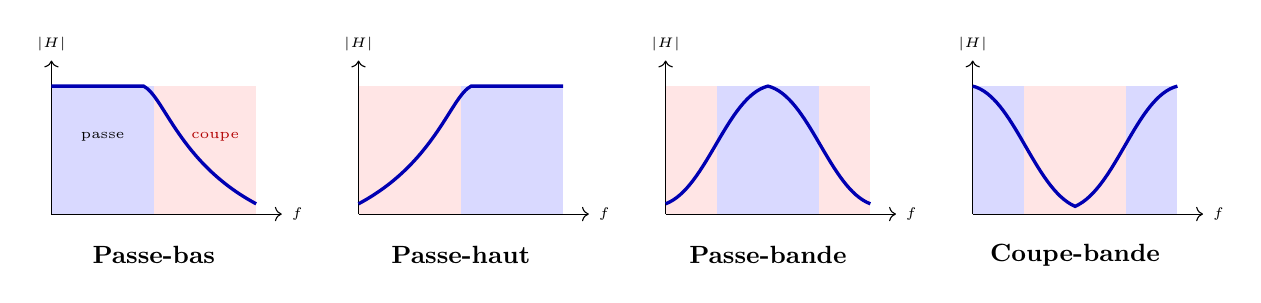
\begin{tikzpicture}[scale=0.65]
  % Passe-bas
  \begin{scope}[shift={(0,0)}]
    \fill[blue!15] (0,0) rectangle (2,2.5);
    \fill[red!10] (2,0) rectangle (4,2.5);
    \draw[->] (0,0) -- (4.5,0) node[right, font=\tiny]{$f$};
    \draw[->] (0,0) -- (0,3) node[above, font=\tiny]{$|H|$};
    \draw[very thick, blue!70!black] (0,2.5) -- (1.8,2.5) .. controls (2.2,2.3) and (2.5,1) .. (4,0.2);
    \node[font=\small\bfseries] at (2,-0.8) {Passe-bas};
    \node[font=\tiny] at (1,1.5) {passe};
    \node[font=\tiny, red!70!black] at (3.2,1.5) {coupe};
  \end{scope}
  % Passe-haut
  \begin{scope}[shift={(6,0)}]
    \fill[red!10] (0,0) rectangle (2,2.5);
    \fill[blue!15] (2,0) rectangle (4,2.5);
    \draw[->] (0,0) -- (4.5,0) node[right, font=\tiny]{$f$};
    \draw[->] (0,0) -- (0,3) node[above, font=\tiny]{$|H|$};
    \draw[very thick, blue!70!black] (0,0.2) .. controls (1.5,1) and (1.8,2.3) .. (2.2,2.5) -- (4,2.5);
    \node[font=\small\bfseries] at (2,-0.8) {Passe-haut};
  \end{scope}
  % Passe-bande
  \begin{scope}[shift={(12,0)}]
    \fill[red!10] (0,0) rectangle (1,2.5);
    \fill[blue!15] (1,0) rectangle (3,2.5);
    \fill[red!10] (3,0) rectangle (4,2.5);
    \draw[->] (0,0) -- (4.5,0) node[right, font=\tiny]{$f$};
    \draw[->] (0,0) -- (0,3) node[above, font=\tiny]{$|H|$};
    \draw[very thick, blue!70!black] (0,0.2) .. controls (0.8,0.5) and (1.2,2.3) .. (2,2.5) .. controls (2.8,2.3) and (3.2,0.5) .. (4,0.2);
    \node[font=\small\bfseries] at (2,-0.8) {Passe-bande};
  \end{scope}
  % Coupe-bande
  \begin{scope}[shift={(18,0)}]
    \fill[blue!15] (0,0) rectangle (1,2.5);
    \fill[red!10] (1,0) rectangle (3,2.5);
    \fill[blue!15] (3,0) rectangle (4,2.5);
    \draw[->] (0,0) -- (4.5,0) node[right, font=\tiny]{$f$};
    \draw[->] (0,0) -- (0,3) node[above, font=\tiny]{$|H|$};
    \draw[very thick, blue!70!black] (0,2.5) .. controls (0.8,2.3) and (1.2,0.5) .. (2,0.15) .. controls (2.8,0.5) and (3.2,2.3) .. (4,2.5);
    \node[font=\small\bfseries] at (2,-0.8) {Coupe-bande};
  \end{scope}
\end{tikzpicture}
\end{center}

\subsection{Filtres passifs du 1er ordre}

Les filtres les plus simples n'utilisent qu'une résistance et un condensateur (ou une bobine).

\textbf{Passe-bas RC :}

\begin{center}
\begin{circuitikz}[scale=0.85]
  \draw (0,0) to[R, l=$R$] (3,0) to[short] (4,0);
  \draw (3,0) to[C, l=$C$] (3,-1.5) node[ground]{};
  \draw[->, blue!70!black, thick] (-0.5,0.3) -- (0.5,0.3) node[midway, above, font=\small]{$v_{\text{in}}$};
  \draw[->, red!70!black, thick] (3.5,0.3) -- (4.5,0.3) node[midway, above, font=\small]{$v_{\text{out}}$};
\end{circuitikz}
\end{center}

\begin{formule}
\[
\underline{H} = \frac{1}{1 + j\omega RC} \qquad f_c = \frac{1}{2\pi RC} \qquad \text{pente : } -\SI{20}{dB/déc}
\]
\end{formule}

\textbf{Passe-haut CR :} on échange $R$ et $C$.

\begin{center}
\begin{circuitikz}[scale=0.85]
  \draw (0,0) to[C, l=$C$] (3,0) to[short] (4,0);
  \draw (3,0) to[R, l=$R$] (3,-1.5) node[ground]{};
  \draw[->, blue!70!black, thick] (-0.5,0.3) -- (0.5,0.3) node[midway, above, font=\small]{$v_{\text{in}}$};
  \draw[->, red!70!black, thick] (3.5,0.3) -- (4.5,0.3) node[midway, above, font=\small]{$v_{\text{out}}$};
\end{circuitikz}
\end{center}

\begin{formule}
\[
\underline{H} = \frac{j\omega RC}{1 + j\omega RC} \qquad f_c = \frac{1}{2\pi RC} \qquad \text{pente BF : } +\SI{20}{dB/déc}
\]
\end{formule}

\begin{intuition}
\textbf{Pourquoi ça filtre ?} En BF, le condensateur a une impédance élevée : il est ``quasi ouvert''. En HF, son impédance est faible : il est ``quasi court-circuit''. Dans le passe-bas, le condensateur est en dérivation vers la masse : en HF, il court-circuite le signal à la masse. Dans le passe-haut, le condensateur est en série : en BF, il bloque le passage.
\end{intuition}

\subsection{Le problème des filtres passifs du 1er ordre}

Un filtre du 1er ordre n'atténue que de $-\SI{20}{dB/décade}$ dans la bande coupée. C'est souvent \textbf{insuffisant}.

\begin{pratique}
\textbf{Exemple :} on veut filtrer un signal audio (bande utile $< \SI{20}{kHz}$) avant un ADC échantillonnant à \SI{48}{kHz}. Il faut rejeter les fréquences au-dessus de $f_s/2 = \SI{24}{kHz}$ pour éviter le repliement (aliasing).

Avec un filtre du 1er ordre ($f_c = \SI{20}{kHz}$), l'atténuation à \SI{24}{kHz} ($0{,}26$ décade au-dessus) n'est que de $\sim\SI{5}{dB}$ : insuffisant.

À \SI{100}{kHz} (si un parasite HF est présent) : $\sim\SI{14}{dB}$. Toujours insuffisant.

Il faut un filtre d'ordre \textbf{supérieur} : 2nd ordre ($-\SI{40}{dB/déc}$), 4e ordre ($-\SI{80}{dB/déc}$), etc.
\end{pratique}

\subsection{Filtres passifs du 2nd ordre : le RLC}

On l'a vu aux chapitres 9 et 12. Le circuit RLC donne un filtre du 2nd ordre avec une pente de $-\SI{40}{dB/décade}$ --- deux fois plus raide que le 1er ordre.

\begin{formule}
\textbf{Passe-bas RLC} (sortie aux bornes de $C$) :
\[
\underline{H} = \frac{1}{1 + j\omega/(Q\omega_0) + (j\omega/\omega_0)^2} \qquad f_0 = \frac{1}{2\pi\sqrt{LC}}
\]
\end{formule}

\begin{attention}
\textbf{Inconvénient majeur des filtres passifs :}
\begin{itemize}[nosep]
\item Ils \textbf{atténuent toujours} le signal (gain $\leq 1$). Pas d'amplification possible.
\item Le 2nd ordre passif nécessite une \textbf{inductance}, composant encombrant, cher, et qui introduit des pertes et des couplages magnétiques parasites. En BF ($< \SI{100}{kHz}$), les inductances deviennent énormes.
\item \textbf{L'impédance de charge modifie le filtre.} Un diviseur résistif en sortie change $f_c$ et $Q$.
\end{itemize}
C'est pourquoi on préfère les \textbf{filtres actifs} en basse fréquence (audio, instrumentation, asservissement).
\end{attention}

\subsection{Pourquoi les filtres actifs ?}

Un filtre actif utilise un \textbf{amplificateur opérationnel} (AOP) en combinaison avec des résistances et des condensateurs. Avantages :

\begin{itemize}[nosep]
\item \textbf{Pas d'inductance} : uniquement $R$ et $C$ $\Rightarrow$ compact et bon marché.
\item \textbf{Gain possible} : le filtre peut amplifier en même temps qu'il filtre.
\item \textbf{Impédance de sortie faible} : la sortie de l'AOP attaque n'importe quelle charge sans modifier le filtre.
\item \textbf{$Q$ ajustable indépendamment} : on peut régler $f_0$ et $Q$ séparément.
\end{itemize}

\begin{retenir}
\textbf{Filtres passifs vs actifs :}
\begin{enumerate}[nosep]
\item 1er ordre : RC ou CR. Simple, mais pente limitée ($-\SI{20}{dB/déc}$).
\item 2nd ordre passif : RLC. Pente $-\SI{40}{dB/déc}$ mais nécessite une inductance.
\item 2nd ordre actif : RC + AOP (Sallen-Key, MFB\ldots). Pas d'inductance, gain et $Q$ réglables.
\item Pour l'ordre $> 2$ : on met en cascade des cellules du 2nd ordre.
\end{enumerate}
\end{retenir}

% ----------------------------------------------------------------------------
\section{Approfondissement}

\begin{approfondissement}
Topologies de filtres actifs, dimensionnement, et réponses normalisées (Butterworth, Bessel, Tchebychev). Prérequis : chapitre 13 (fonctions de transfert du 2nd ordre), notion d'AOP idéal.
\end{approfondissement}

\subsection{La topologie Sallen-Key}

C'est la topologie de filtre actif la plus utilisée pour le 2nd ordre. L'AOP est monté en \textbf{suiveur} (gain unitaire) ou en non-inverseur (gain $> 1$).

\textbf{Passe-bas Sallen-Key (gain unitaire) :}

\begin{center}
\begin{circuitikz}[scale=0.85]
  \draw (0,0) to[R, l=$R_1$] (2.5,0) to[R, l=$R_2$] (5,0);
  \draw (5,0) -- (5.5,0);
  % C2 vers masse
  \draw (2.5,0) to[C, l_=$C_2$] (2.5,-1.5) node[ground]{};
  % C1 de la jonction R2/entrée+ vers sortie
  \draw (5,0) to[C, l=$C_1$] (5,-1.5) node[ground]{};
  % AOP
  \draw (5.5,0.3) node[op amp, anchor=+, scale=0.6](AOP){};
  \draw (AOP.-) -- ++(0,-0.8) -| (AOP.out);
  \draw (AOP.out) -- ++(0.8,0) node[right]{$v_{\text{out}}$};
  % Feedback C1
  \draw (5,0) -- (5,1.2) -| (AOP.out);
  % Labels
  \draw[->, blue!70!black, thick] (-0.7,0.3) -- (0.3,0.3) node[midway, above, font=\small]{$v_{\text{in}}$};
\end{circuitikz}
\end{center}

\begin{attention}
Le schéma ci-dessus est une version simplifiée. Dans la topologie Sallen-Key complète, $C_1$ est connecté entre la sortie de $R_2$ et la sortie de l'AOP (rétroaction positive via $C_1$), ce qui est essentiel pour obtenir un $Q > 0{,}5$ sans inductance.
\end{attention}

\begin{formule}
Pour un Sallen-Key passe-bas avec composants égaux ($R_1 = R_2 = R$, gain unitaire) :
\[
f_0 = \frac{1}{2\pi R\sqrt{C_1 C_2}} \qquad Q = \frac{\sqrt{C_1 C_2}}{C_1 + C_2}\cdot\frac{1}{1} = \frac{\sqrt{C_1/C_2}}{1 + C_1/C_2}
\]
Pour un filtre Butterworth ($Q = 0{,}707$) avec $R_1 = R_2 = R$ : choisir $C_1/C_2 = 2$, par exemple $C_1 = \SI{2.2}{nF}$, $C_2 = \SI{1}{nF}$.
\end{formule}

\subsection{La topologie MFB (Multiple Feedback)}

La topologie MFB (ou Rauch) utilise l'AOP en \textbf{inverseur}. Elle est plus sensible aux tolérances des composants que la Sallen-Key, mais offre un meilleur comportement en HF (pas de rétroaction positive).

\begin{pratique}
\textbf{Quand utiliser quoi :}
\begin{itemize}[nosep]
\item \textbf{Sallen-Key} : gain unitaire ou faible gain, $Q < 10$, simple à concevoir. Choix par défaut.
\item \textbf{MFB} : gain inverseur, meilleur pour $Q$ élevé, meilleur rejet HF. Utilisé en audio de précision.
\item \textbf{State-variable} : permet de sortir simultanément PB, PH et PBande depuis le même circuit. Utilisé en synthétiseurs audio et en instrumentation.
\item \textbf{Biquad} : grande flexibilité, composants indépendants pour $f_0$, $Q$ et gain. Utilisé dans les filtres programmables.
\end{itemize}
\end{pratique}

\subsection{Réponses normalisées : Butterworth, Bessel, Tchebychev}

Le choix de la \textbf{réponse normalisée} détermine la forme de la courbe de gain dans la bande passante et la transition vers la bande coupée.

\begin{center}
\renewcommand{\arraystretch}{1.5}
\begin{tabular}{p{2.8cm}p{2.5cm}p{2.5cm}p{4.5cm}}
\toprule
\textbf{Type} & \textbf{Bande passante} & \textbf{Transition} & \textbf{Usage typique} \\
\midrule
\textbf{Butterworth} & Maximalement plate & Moyenne & Usage général, audio \\
\textbf{Bessel} & Quasi plate & Douce & Transmission de données, impulsions \\
\textbf{Tchebychev I} & Ondulation (ripple) & Raide & Réjection forte, télécoms \\
\textbf{Tchebychev II} & Plate & Raide (ondulation en bande coupée) & Filtrage RF \\
\textbf{Elliptique (Cauer)} & Ondulation & Très raide & Réjection maximale, espace minimal \\
\bottomrule
\end{tabular}
\end{center}

\begin{intuition}
\textbf{Le compromis fondamental :} il est \textbf{impossible} d'avoir simultanément une bande passante parfaitement plate, une transition infiniment raide, et une phase parfaitement linéaire. Chaque type de filtre sacrifie un aspect pour optimiser les autres :
\begin{itemize}[nosep]
\item Butterworth sacrifie la raideur pour la platitude.
\item Bessel sacrifie la raideur pour la linéarité de phase (préserve la forme des signaux).
\item Tchebychev sacrifie la platitude pour la raideur.
\item Elliptique pousse le compromis au maximum : transition la plus raide pour un ordre donné, mais ondulation partout.
\end{itemize}
\end{intuition}

\subsection{Tables de dimensionnement du 2nd ordre}

Pour un filtre passe-bas du 2nd ordre de fréquence de coupure $f_c$, les valeurs de $Q$ sont :

\begin{center}
\begin{tabular}{lcc}
\toprule
\textbf{Type} & \textbf{$Q$ (2nd ordre)} & \textbf{Dépassement transitoire} \\
\midrule
Bessel & $0{,}577$ & $0{,}4\%$ \\
Butterworth & $0{,}707$ & $4{,}3\%$ \\
Tchebychev 0,5\,dB & $0{,}864$ & $13\%$ \\
Tchebychev 1\,dB & $0{,}957$ & $21\%$ \\
Tchebychev 3\,dB & $1{,}306$ & $39\%$ \\
\bottomrule
\end{tabular}
\end{center}

\subsection{Filtres d'ordre supérieur par cascade}

Pour obtenir un filtre d'ordre $n > 2$, on met en \textbf{cascade} des cellules du 2nd ordre (et une cellule du 1er ordre si $n$ est impair). Chaque cellule a son propre $Q_k$ et sa propre $f_{0,k}$, calculés à partir de tables.

\begin{formule}
\textbf{Butterworth d'ordre $n$} : $n/2$ cellules du 2nd ordre (si $n$ pair) avec des $Q_k$ donnés par :
\[
Q_k = \frac{1}{2\sin\left(\frac{(2k-1)\pi}{2n}\right)} \qquad k = 1, 2, \ldots, n/2
\]
Toutes les cellules ont la même $f_0 = f_c$.
\end{formule}

\begin{pratique}
\textbf{Valeurs de $Q$ pour Butterworth :}
\begin{center}
\begin{tabular}{cl}
\toprule
\textbf{Ordre} & \textbf{$Q$ des cellules} \\
\midrule
2 & $0{,}707$ \\
3 & $1{,}000$ + 1er ordre \\
4 & $0{,}541$ et $1{,}307$ \\
5 & $0{,}618$ et $1{,}618$ + 1er ordre \\
6 & $0{,}518$, $0{,}707$ et $1{,}932$ \\
\bottomrule
\end{tabular}
\end{center}
\textbf{Attention :} la cellule de plus haut $Q$ domine la réponse transitoire. Pour un Butterworth d'ordre 6, la cellule à $Q = 1{,}932$ a un pic de résonance de $\sim\SI{6}{dB}$ --- elle doit être placée en \textit{dernier} dans la cascade pour ne pas saturer les étages suivants.
\end{pratique}

\subsection{Exemple de dimensionnement complet}

\begin{pratique}
\textbf{Cahier des charges :} filtre anti-aliasing pour un ADC audio, $f_c = \SI{20}{kHz}$, atténuation $>\SI{60}{dB}$ à \SI{100}{kHz}, réponse Butterworth.

\textbf{1. Choix de l'ordre :} à \SI{100}{kHz}, on est à $100/20 = 5\times f_c$ ($0{,}7$ décade). Atténuation Butterworth d'ordre $n$ : $\sim n \times \SI{20}{dB}$ par décade.

Plus précisément, à $f/f_c = 5$ : $|H| = 1/\sqrt{1+(f/f_c)^{2n}} = 1/\sqrt{1+5^{2n}}$.

\begin{tabular}{ll}
$n=3$ : $|H| = 1/\sqrt{1+15625} \approx \SI{-42}{dB}$ & Insuffisant \\
$n=4$ : $|H| = 1/\sqrt{1+390625} \approx \SI{-56}{dB}$ & Presque \\
$n=5$ : $|H| = 1/\sqrt{1+9{,}77\times10^6} \approx \SI{-70}{dB}$ & OK \\
\end{tabular}

$\Rightarrow$ \textbf{Ordre 5} (2 cellules du 2nd ordre + 1 cellule du 1er ordre).

\textbf{2. Valeurs de $Q$ :} Butterworth ordre 5 $\Rightarrow$ $Q_1 = 0{,}618$, $Q_2 = 1{,}618$, + 1 cellule RC.

\textbf{3. Dimensionnement :} toutes les cellules ont $f_0 = f_c = \SI{20}{kHz}$. Pour chaque cellule Sallen-Key avec $R_1 = R_2 = R$ :

Choisissons $R = \SI{3.3}{k\ohm}$ (valeur E24 pratique).

$C_{\text{ref}} = 1/(2\pi R f_0) = 1/(2\pi\times3300\times20000) = \SI{2.41}{nF}$.

Cellule 1 ($Q_1 = 0{,}618$) : $C_1 = 2Q \times C_{\text{ref}} = 1{,}236\times2{,}41 = \SI{2.98}{nF}$ $\to$ \SI{3.3}{nF} (E24).

$C_2 = C_{\text{ref}}/(2Q) = 2{,}41/1{,}236 = \SI{1.95}{nF}$ $\to$ \SI{2.2}{nF} (E24).

Cellule 2 ($Q_2 = 1{,}618$) : $C_1 = 2\times1{,}618\times2{,}41 = \SI{7.80}{nF}$ $\to$ \SI{8.2}{nF} (E24).

$C_2 = 2{,}41/(2\times1{,}618) = \SI{0.745}{nF}$ $\to$ \SI{820}{pF} (E24).

Cellule RC : $C = 1/(2\pi R f_c) = \SI{2.41}{nF}$ $\to$ \SI{2.2}{nF}.

\textbf{4. Vérification :} simuler le circuit complet dans SPICE et vérifier que l'atténuation atteint bien $\SI{-60}{dB}$ à \SI{100}{kHz} malgré les arrondis sur les valeurs de composants.
\end{pratique}

% ----------------------------------------------------------------------------
\section{Niveau Ingénieur}

\begin{ingenieur}
Sensibilité aux composants, filtres à capacités commutées, conception en RF, et considérations pratiques avancées.
\end{ingenieur}

\subsection{Sensibilité aux tolérances des composants}

En pratique, les résistances ont une tolérance de $\pm1\%$ à $\pm5\%$ et les condensateurs de $\pm5\%$ à $\pm20\%$. Ces dispersions décalent $f_0$ et $Q$ par rapport aux valeurs théoriques.

\begin{formule}
La \textbf{sensibilité} de $f_0$ par rapport à un composant $x$ est :
\[
S_x^{f_0} = \frac{\partial f_0 / f_0}{\partial x / x} = \frac{x}{f_0}\frac{\partial f_0}{\partial x}
\]
Pour un filtre RC : $f_0 = 1/(2\pi RC)$, donc $S_R^{f_0} = -1$ et $S_C^{f_0} = -1$. Une variation de $+5\%$ sur $R$ décale $f_0$ de $-5\%$.

Pour un filtre Sallen-Key, la sensibilité de $Q$ aux composants peut être très élevée (surtout pour $Q > 5$). C'est pourquoi les topologies state-variable et biquad sont préférées quand $Q$ doit être précis.
\end{formule}

\begin{pratique}
\textbf{Règles de conception :}
\begin{itemize}[nosep]
\item Utiliser des résistances à $\pm1\%$ (série E96) pour les filtres de précision.
\item Utiliser des condensateurs \textbf{C0G/NP0} (céramique classe I, $\pm5\%$, stables en température et en tension) pour les applications critiques (audio, instrumentation).
\item Éviter les X7R/X5R dans les filtres de précision (capacité varie avec la tension DC et la température).
\item Pour $Q > 10$ : préférer les topologies state-variable ou biquad (faible sensibilité).
\item \textbf{Toujours simuler} avec des tolérances (analyse Monte Carlo dans SPICE) avant de fabriquer.
\end{itemize}
\end{pratique}

\subsection{Filtres à capacités commutées (switched-capacitor)}

Les filtres à capacités commutées remplacent les résistances par des \textbf{condensateurs commutés à haute fréquence}. L'avantage : la fréquence de coupure est déterminée par le \textbf{rapport de capacités} (très précis en technologie CMOS, $\pm 0{,}1\%$) et par la \textbf{fréquence d'horloge} (précise au quartz).

\begin{formule}
Un condensateur $C_s$ commuté à la fréquence $f_{\text{clk}}$ se comporte comme une résistance équivalente :
\[
R_{\text{éq}} = \frac{1}{C_s \cdot f_{\text{clk}}}
\]
En changeant $f_{\text{clk}}$, on change $f_c$ du filtre sans toucher aux composants.
\end{formule}

\begin{pratique}
\textbf{Circuits intégrés courants :} MAX291/MAX292, LTC1068, MF10. Ils intègrent un filtre d'ordre 4 à 8 dont la fréquence de coupure est fixée par une horloge externe : $f_c = f_{\text{clk}}/50$ ou $/100$ typiquement.

\textbf{Avantages :} $f_c$ ajustable, précis, intégrable en CMOS.

\textbf{Inconvénients :} le signal est échantillonné à $f_{\text{clk}}$ --- il faut un filtre anti-aliasing \textit{analogique} en amont. Et l'horloge injecte du bruit à $f_{\text{clk}}$ (clock feedthrough).
\end{pratique}

\subsection{Filtres passifs en RF et puissance}

Au-dessus de quelques MHz, les filtres actifs ne fonctionnent plus (la bande passante de l'AOP est insuffisante). On revient aux \textbf{filtres passifs} LC :

\begin{pratique}
\textbf{Topologies classiques en RF :}
\begin{itemize}[nosep]
\item \textbf{Filtre en $\pi$} : $C$-$L$-$C$ (shunt-série-shunt). Impédance d'entrée et de sortie élevées.
\item \textbf{Filtre en T} : $L$-$C$-$L$ (série-shunt-série). Impédance d'entrée et de sortie faibles.
\item \textbf{Filtre en échelle} : cascade de sections en $\pi$ ou en T. Utilisé pour les filtres d'ordre élevé.
\end{itemize}

\textbf{En puissance} (filtrage EMI, alimentation) :
\begin{itemize}[nosep]
\item \textbf{Filtre LC en $\pi$} sur les entrées secteur (norme EMI).
\item \textbf{Filtre de sortie LC} des convertisseurs buck/boost (lisse l'ondulation de commutation).
\item \textbf{Common-mode choke} + condensateurs Y pour le mode commun.
\end{itemize}
\end{pratique}

\subsection{Limites des filtres analogiques et transition vers le numérique}

\begin{attention}
Les filtres analogiques ont des limites fondamentales :
\begin{itemize}[nosep]
\item \textbf{Dérive avec la température} : $R$, $C$, $L$ changent $\Rightarrow$ $f_c$ et $Q$ dérivent.
\item \textbf{Ordre limité} : au-delà de l'ordre 8--10, la cascade de cellules accumule les imprécisions et le bruit.
\item \textbf{Pas de réponse à phase linéaire parfaite} : même le Bessel n'est que ``quasi linéaire''.
\item \textbf{Pas reconfigurable} : changer $f_c$ nécessite de changer des composants (sauf switched-cap).
\end{itemize}

Pour les applications exigeantes (audio haute fidélité, télécoms, radar), on préfère souvent un filtre \textbf{numérique} (FIR ou IIR) implémenté dans un DSP ou un FPGA. Le filtre analogique subsiste en amont comme \textbf{anti-aliasing} avant l'ADC, et en aval comme \textbf{filtre de reconstruction} après le DAC.
\end{attention}

% === EXERCICES DU CHAPITRE 14 ===
\section*{Exercices}
\addcontentsline{toc}{section}{Exercices}

\subsection*{Niveau débutant}

\textbf{Exercice 14.1 ---} On veut un filtre passe-bas RC avec $f_c = \SI{1}{kHz}$. Si $C = \SI{100}{nF}$, quelle résistance choisir ? Quel est le gain à \SI{10}{kHz} ?

\begin{pratique}
\textbf{Solution :} $R = 1/(2\pi f_c C) = 1/(2\pi\times10^3\times10^{-7}) = \SI{1592}{\ohm}$ $\to$ \SI{1.5}{k\ohm} (E24).

À \SI{10}{kHz} ($= 10f_c$) : $G \approx -\SI{20}{dB}$ ($= \div 10$). Exact : $|H| = 1/\sqrt{1+100} = 0{,}0995$ soit $\SI{-20.0}{dB}$.
\end{pratique}

\textbf{Exercice 14.2 ---} Un signal contient une composante utile à \SI{50}{Hz} et un parasite à \SI{50}{kHz}. On veut atténuer le parasite de \SI{40}{dB}. Un filtre du 1er ordre suffit-il ?

\begin{pratique}
\textbf{Solution :} Rapport de fréquences : $50000/50 = 1000 = 3$ décades.

1er ordre : $3 \times \SI{20}{dB} = \SI{60}{dB}$. Oui, un 1er ordre avec $f_c$ entre \SI{50}{Hz} et \SI{50}{kHz} suffit.

Choisissons $f_c = \SI{500}{Hz}$. À \SI{50}{kHz} : $f/f_c = 100 = 2$ décades $\Rightarrow$ $\SI{-40}{dB}$. OK.

Le signal utile à \SI{50}{Hz} est à $0{,}1 \times f_c$ : gain $\approx \SI{0}{dB}$ (quasi pas d'atténuation). \checkmark
\end{pratique}

\subsection*{Niveau intermédiaire}

\textbf{Exercice 14.3 ---} Dimensionnez un filtre Sallen-Key passe-bas Butterworth du 2nd ordre avec $f_c = \SI{10}{kHz}$ et $R_1 = R_2 = \SI{10}{k\ohm}$. Calculez $C_1$ et $C_2$.

\begin{pratique}
\textbf{Solution :} Butterworth $\Rightarrow$ $Q = 0{,}707$. Avec $R_1 = R_2 = R$ :

$C_{\text{ref}} = 1/(2\pi R f_c) = 1/(2\pi\times10^4\times10^4) = \SI{1.59}{nF}$.

$C_1 = 2Q \times C_{\text{ref}} = 2\times0{,}707\times1{,}59 = \SI{2.25}{nF}$ $\to$ \SI{2.2}{nF} (E24).

$C_2 = C_{\text{ref}}/(2Q) = 1{,}59/(2\times0{,}707) = \SI{1.12}{nF}$ $\to$ \SI{1}{nF} (E24).

Vérification : $f_0 = 1/(2\pi R\sqrt{C_1 C_2}) = 1/(2\pi\times10^4\times\sqrt{2{,}2\times10^{-9}\times10^{-9}})$

$= 1/(2\pi\times10^4\times1{,}483\times10^{-9}) = \SI{10.7}{kHz}$. Proche de \SI{10}{kHz} (\checkmark, l'arrondi E24 décale légèrement).
\end{pratique}

\textbf{Exercice 14.4 ---} On met en cascade un passe-haut CR ($f_c = \SI{20}{Hz}$) et un passe-bas RC ($f_c = \SI{20}{kHz}$) avec un buffer entre les deux. Quel est le type de filtre résultant ? Quelle est la bande passante ? Tracez le diagramme de Bode asymptotique.

\begin{pratique}
\textbf{Solution :} C'est un \textbf{filtre passe-bande} du 1er ordre par côté : il laisse passer entre \SI{20}{Hz} et \SI{20}{kHz} (bande audio).

Bode asymptotique : montée à $+\SI{20}{dB/déc}$ de \SI{20}{Hz} à \SI{20}{Hz}, plateau à \SI{0}{dB} de \SI{20}{Hz} à \SI{20}{kHz}, descente à $-\SI{20}{dB/déc}$ au-dessus de \SI{20}{kHz}.

Bande passante à $-\SI{3}{dB}$ : de \SI{20}{Hz} à \SI{20}{kHz} (exactement la bande audio).

$G_{\text{total}} = G_{\text{PH}} + G_{\text{PB}}$ (en dB). Les phases s'additionnent aussi.
\end{pratique}

\subsection*{Niveau ingénieur}

\textbf{Exercice 14.5 ---} Un filtre anti-aliasing Butterworth d'ordre 4 doit avoir $f_c = \SI{48}{kHz}$ pour un ADC à \SI{192}{kHz}. Calculez l'atténuation à $f_s/2 = \SI{96}{kHz}$. Donnez les $Q$ des deux cellules du 2nd ordre. Avec $R = \SI{1}{k\ohm}$, dimensionnez les condensateurs de chaque cellule Sallen-Key.

\begin{pratique}
\textbf{Solution :} À $f/f_c = 96/48 = 2$ :

$|H| = 1/\sqrt{1+2^8} = 1/\sqrt{257} = 0{,}0623$ soit $\SI{-24}{dB}$.

Butterworth ordre 4 : $Q_1 = 0{,}541$ et $Q_2 = 1{,}307$.

$C_{\text{ref}} = 1/(2\pi\times10^3\times48000) = \SI{3.32}{nF}$.

\textbf{Cellule 1} ($Q_1 = 0{,}541$) :

$C_1 = 2\times0{,}541\times3{,}32 = \SI{3.59}{nF}$ $\to$ \SI{3.3}{nF}.

$C_2 = 3{,}32/(2\times0{,}541) = \SI{3.07}{nF}$ $\to$ \SI{3.3}{nF}.

\textbf{Cellule 2} ($Q_2 = 1{,}307$) :

$C_1 = 2\times1{,}307\times3{,}32 = \SI{8.68}{nF}$ $\to$ \SI{8.2}{nF}.

$C_2 = 3{,}32/(2\times1{,}307) = \SI{1.27}{nF}$ $\to$ \SI{1.2}{nF}.

Ordre de cascade : cellule 1 (faible $Q$) en premier, cellule 2 (haut $Q$) en dernier pour éviter la saturation interne.
\end{pratique}

\textbf{Exercice 14.6 ---} Un filtre passe-bande passif LC pour un récepteur à \SI{433}{MHz} a $L = \SI{22}{nH}$ et $C = \SI{6.2}{pF}$. Calculez $f_0$. La bobine a un $Q_L = 40$ (résistance série $R_L$). La source et la charge sont de \SI{50}{\ohm}. Calculez le $Q$ en charge et la bande passante.

\begin{pratique}
\textbf{Solution :} $f_0 = 1/(2\pi\sqrt{22\times10^{-9}\times6{,}2\times10^{-12}}) = 1/(2\pi\times\SI{1.168e-10}{})$

$= 1/(7{,}34\times10^{-10}) \approx \SI{432}{MHz}$. \checkmark{} (proche de \SI{433}{MHz}).

$R_L = \omega_0 L/Q_L = 2\pi\times433\times10^6\times22\times10^{-9}/40 = \SI{1.50}{\ohm}$.

Résistance totale du circuit : $R_{\text{tot}} = R_L + R_s + R_{\text{charge}}$. Ici, en circuit série : $R_{\text{tot}} = 1{,}5 + 50 + 50 = \SI{101.5}{\ohm}$.

$Q_L = (1/R_{\text{tot}})\sqrt{L/C} = (1/101{,}5)\sqrt{22\times10^{-9}/6{,}2\times10^{-12}} = (1/101{,}5)\times59{,}6 = 0{,}587$.

$\Delta f = f_0/Q_L = 433/0{,}587 \approx \SI{738}{MHz}$. Le filtre est \textbf{totalement sur-amorti} --- les impédances source/charge de \SI{50}{\ohm} ``écrasent'' le $Q$ du résonateur. Il faut un \textbf{réseau d'adaptation} (cf.\ chapitre 12) ou un couplage faible pour préserver la sélectivité.
\end{pratique}

\subsection*{Questions de compréhension}

\begin{enumerate}[nosep]
\item Pourquoi préfère-t-on les filtres actifs aux filtres passifs en dessous de \SI{100}{kHz} ? Qu'est-ce qui change au-dessus ?
\item Un filtre Butterworth et un filtre Tchebychev de même ordre ont la même $f_c$. Lequel atténue le plus à $2f_c$ ? Lequel a la meilleure réponse en transitoire ? Pourquoi ?
\item On cascade trois cellules passe-bas du 1er ordre identiques ($f_c = \SI{1}{kHz}$). Le filtre résultant a-t-il le même comportement qu'un Butterworth d'ordre 3 ? Si non, quelle est la différence ?
\item Expliquez pourquoi un filtre à capacités commutées nécessite un filtre anti-aliasing analogique en amont.
\end{enumerate}

% === RÉSUMÉ DU CHAPITRE 14 ===
\section*{Résumé du chapitre}
\addcontentsline{toc}{section}{Résumé du chapitre}

\begin{bases}[title={\color{white} Résumé --- Les Bases}]
\begin{center}
\renewcommand{\arraystretch}{1.3}
\begin{tabular}{p{4cm}p{9cm}}
\toprule
1er ordre (RC/CR) & $f_c = 1/(2\pi RC)$, pente $\pm\SI{20}{dB/déc}$ \\
2nd ordre passif & RLC : pente $\pm\SI{40}{dB/déc}$, nécessite une inductance \\
Filtre actif & RC + AOP : pas d'inductance, gain possible, $Q$ réglable \\
Ordre supérieur & Cascade de cellules du 2nd ordre \\
\bottomrule
\end{tabular}
\end{center}
\end{bases}

\begin{approfondissement}[title={\color{white} Résumé --- Approfondissement}]
\begin{center}
\renewcommand{\arraystretch}{1.3}
\begin{tabular}{p{4cm}p{9cm}}
\toprule
Sallen-Key & Topologie la plus courante (suiveur ou non-inverseur) \\
MFB & Inverseur, meilleur pour $Q$ élevé et rejet HF \\
Butterworth & $Q = 0{,}707$ (2nd ordre), maximalement plat \\
Bessel & Phase linéaire, préserve les impulsions \\
Tchebychev & Transition raide, mais ondulation en bande passante \\
\bottomrule
\end{tabular}
\end{center}
\end{approfondissement}

\begin{ingenieur}[title={\color{white} Résumé --- Niveau Ingénieur}]
\begin{center}
\renewcommand{\arraystretch}{1.3}
\begin{tabular}{p{4cm}p{9cm}}
\toprule
Sensibilité & $S_x^{f_0}$ mesure l'impact des tolérances --- critique pour $Q$ élevé \\
Switched-cap & $R_{\text{éq}} = 1/(C_s f_{\text{clk}})$ --- $f_c$ contrôlé par horloge \\
RF / puissance & Filtres LC passifs : topologies $\pi$, T, échelle \\
Numérique & FIR/IIR dans DSP/FPGA pour les besoins exigeants \\
\bottomrule
\end{tabular}
\end{center}
\end{ingenieur}


% ============================================================================
% PARTIE V : SEMI-CONDUCTEURS
% ============================================================================
\part{Semi-conducteurs}

% ============================================================================
% CHAPITRE 15 : LA DIODE
% ============================================================================
\chapter{La Diode}

\begin{center}
\textit{La diode est le composant semi-conducteur le plus simple :\\
elle laisse passer le courant dans un sens et le bloque dans l'autre.\\
C'est le premier composant non-linéaire du livre,\\
et la porte d'entrée vers toute l'électronique à semi-conducteurs.}
\end{center}

\vspace{0.5cm}

Jusqu'ici, tous les composants étudiés étaient \textbf{linéaires} : la relation entre tension et courant était proportionnelle (résistance) ou différentielle linéaire (condensateur, bobine). La diode rompt cette symétrie : son comportement dépend du \textit{signe} de la tension appliquée. C'est ce qui permet le redressement, la protection, la détection et bien d'autres fonctions essentielles.

% ----------------------------------------------------------------------------
\section{Les Bases}

\begin{bases}
Cette section présente la diode de manière intuitive et pratique, sans entrer dans la physique des semi-conducteurs. Prérequis : chapitres 1 à 3 (courant, tension, résistance).
\end{bases}

\subsection{Qu'est-ce qu'une diode ?}

Une diode est un composant à \textbf{deux bornes} (un dipôle) qui conduit le courant dans un seul sens.

\begin{itemize}[nosep]
\item L'\textbf{anode} (A) : borne ``$+$'' de la diode.
\item La \textbf{cathode} (K) : borne ``$-$'', marquée par un trait ou une bande sur le boîtier.
\end{itemize}

\begin{center}
\begin{circuitikz}[scale=1.2]
  \draw (0,0) -- (0.8,0) to[D, l=$D$, v=$V_D$] (3.2,0) -- (4,0);
  \draw[-{Stealth[length=2.5mm]}, blue!70!black, thick] (0,0.05) -- (0.6,0.05);
  \node[blue!70!black, above, font=\small] at (0.3,0.1) {$I_D$};
  \node[below, font=\small] at (0,-0.15) {A};
  \node[below, font=\small] at (4,-0.15) {K};
\end{circuitikz}
\end{center}

\begin{analogie}
\textbf{Le clapet anti-retour.} Une diode est comme un clapet dans un tuyau d'eau :
\begin{itemize}[nosep]
\item Dans le \textbf{sens passant} (anode $\to$ cathode) : le clapet s'ouvre et l'eau (le courant) circule. Mais il faut une pression minimale pour ouvrir le clapet $\Rightarrow$ c'est la \textbf{tension de seuil} $V_F$.
\item Dans le \textbf{sens bloqué} (cathode $\to$ anode) : le clapet est fermé. Rien ne passe (ou presque).
\end{itemize}
\textit{Limite :} si la pression inverse est trop forte, le clapet cède $\Rightarrow$ c'est le \textbf{claquage} (tension inverse maximale).
\end{analogie}

\subsection{Les deux régimes de fonctionnement}

\begin{formule}
\textbf{Polarisation directe} ($V_D > 0$, anode plus positive que cathode) :
\begin{itemize}[nosep]
\item Si $V_D < V_F$ (tension de seuil) : la diode est \textbf{bloquée}. Très peu de courant passe.
\item Si $V_D \geq V_F$ : la diode \textbf{conduit}. Le courant circule de l'anode vers la cathode. La tension aux bornes reste approximativement $V_F$.
\end{itemize}

\textbf{Polarisation inverse} ($V_D < 0$) :
\begin{itemize}[nosep]
\item La diode est \textbf{bloquée}. Un courant de fuite infime circule ($\sim$ nA à $\mu$A selon la technologie).
\item Si $|V_D|$ dépasse la \textbf{tension de claquage} $V_{BR}$ : la diode conduit brutalement en inverse (destruction si non prévue).
\end{itemize}
\end{formule}

\subsection{Tension de seuil selon la technologie}

\begin{center}
\begin{tabular}{lll}
\toprule
\textbf{Type de diode} & \textbf{$V_F$ typique} & \textbf{Usage principal} \\
\midrule
Silicium (Si) standard & $\sim\SI{0.7}{V}$ & Redressement, usage général \\
Schottky & $\SI{0.2}{V}$ à $\SI{0.4}{V}$ & Redressement rapide, alimentation \\
Germanium (Ge) & $\sim\SI{0.3}{V}$ & Détection radio (historique) \\
LED rouge & $\sim\SI{1.8}{V}$ & Signalisation \\
LED blanche/bleue & $\sim\SI{3.0}{V}$ & Éclairage \\
\bottomrule
\end{tabular}
\end{center}

\subsection{La caractéristique $I(V)$}

La courbe courant-tension d'une diode est \textbf{fortement non-linéaire} :

\begin{center}
\begin{tikzpicture}[scale=1.0]
  % Axes
  \draw[-{Stealth[length=2.5mm]}] (-4.2,0) -- (4.5,0) node[right, font=\small]{$V_D$ (V)};
  \draw[-{Stealth[length=2.5mm]}] (0,-2.5) -- (0,4.5) node[above, font=\small]{$I_D$ (mA)};
  
  % Graduations axe V
  \draw (1,0.06) -- (1,-0.06);
  \draw (2,0.06) -- (2,-0.06);
  \node[below, font=\footnotesize] at (1,-0.12) {$0{,}5$};
  \node[below, font=\footnotesize] at (2,-0.12) {$V_F$};
  
  % Graduations axe I
  \node[left, font=\footnotesize] at (-0.1,2) {$10$};
  \node[left, font=\footnotesize] at (-0.1,4) {$20$};
  \draw (-0.06,2) -- (0.06,2);
  \draw (-0.06,4) -- (0.06,4);
  
  % Courbe continue : inverse + directe (une seule commande pour éviter discontinuité)
  % Inverse : quasi 0 de -2.8 à 0
  \draw[very thick, blue!70!black, domain=-2.8:0, samples=80, smooth]
    plot(\x, {-0.04});
  % Directe : exponentielle de 0 à ~2
  \draw[very thick, blue!70!black, domain=0:2.0, samples=150, smooth]
    plot(\x, {0.005*(exp(3.5*\x) - 1)});
  % Directe au-delà : quasi verticale
  \draw[very thick, blue!70!black, domain=2.0:2.8, samples=50, smooth]
    plot(\x, {0.005*(exp(3.5*2.0)-1) + 5.5*(\x-2.0)});
  % Raccord inverse à 0 (petit trait pour fermer)
  \draw[very thick, blue!70!black] (-2.8,-0.04) -- (-3.3,-0.04);
  
  % Claquage inverse : courbe lisse
  \draw[very thick, red!70!black, domain=-3.3:-3.9, samples=80, smooth]
    plot(\x, {-0.04 - 3.5*(1 - exp(5*(\x+3.3)))});
  
  % Annotation claquage
  \draw[dashed, gray!50] (-3.3,0) -- (-3.3,-2);
  \node[above, font=\footnotesize] at (-3.3,0.15) {$-V_{BR}$};
  \node[red!70!black, font=\small\bfseries] at (-3.7,-2.3) {Claquage};
  
  % Annotation directe
  \draw[dashed, gray!40] (2,0) -- (2,4);
  \node[blue!70!black, font=\small\bfseries] at (3.5,3) {Directe};
  \node[blue!70!black, font=\small\bfseries] at (-1.8,0.6) {Inverse};
  
  % Annotation coude
  \draw[->, thick, gray!60!black] (3.2,1.2) -- (2.15,0.55);
  \node[gray!60!black, font=\footnotesize, right] at (3.2,1.2) {coude $\approx V_F$};
  
  % Courant de fuite
  \draw[->, thin, gray!50] (-1.5,-0.04) -- (-1.5,-0.6);
  \node[gray!50!black, font=\footnotesize] at (-1.5,-0.85) {$I_S$ (nA)};
\end{tikzpicture}
\end{center}

\begin{intuition}
\textbf{Ce qu'il faut retenir de cette courbe :}
\begin{itemize}[nosep]
\item \textbf{En direct :} rien ne se passe jusqu'à $\sim V_F$, puis le courant ``explose'' exponentiellement. La tension reste quasiment bloquée à $V_F$ quelle que soit l'augmentation du courant.
\item \textbf{En inverse :} quasi rien (courant de fuite $I_S$ infime).
\item \textbf{En claquage inverse :} au-delà de $V_{BR}$, le courant augmente brutalement en inverse. C'est destructeur pour une diode classique, mais c'est le \textbf{principe de fonctionnement} de la diode Zener.
\end{itemize}
\end{intuition}

\subsection{Modèles simplifiés de la diode}

Pour les calculs pratiques, on n'utilise \textit{jamais} l'équation exponentielle directement. On utilise des modèles simplifiés :

\begin{formule}
\textbf{Modèle idéal} (le plus simple) :
\begin{itemize}[nosep]
\item Directe : $V_D = 0$, la diode est un \textbf{court-circuit}.
\item Inverse : $I_D = 0$, la diode est un \textbf{circuit ouvert}.
\end{itemize}

\textbf{Modèle à seuil} (le plus courant en pratique) :
\begin{itemize}[nosep]
\item Directe : $V_D = V_F$ constant (\SI{0.7}{V} pour le Si). La diode est une source de tension.
\item Inverse : $I_D = 0$.
\end{itemize}

\textbf{Modèle à seuil + résistance} (plus précis) :
\begin{itemize}[nosep]
\item Directe : $V_D = V_F + r_D \cdot I_D$, avec $r_D$ la résistance dynamique.
\item Inverse : $I_D = 0$.
\end{itemize}
\end{formule}

\begin{pratique}
\textbf{Quel modèle utiliser ?}
\begin{itemize}[nosep]
\item \textbf{Idéal} : pour comprendre le principe d'un circuit (redressement, portes logiques).
\item \textbf{À seuil ($V_F = \SI{0.7}{V}$)} : pour les calculs à la main, les examens, et le dimensionnement rapide. C'est le modèle par défaut.
\item \textbf{$V_F + r_D$} : quand la chute de tension exacte compte (alimentations de puissance, mesure de courant).
\item \textbf{Exponentiel (Shockley)} : en simulation SPICE uniquement.
\end{itemize}
\end{pratique}

\subsection{Circuit fondamental : la diode en série avec une résistance}

Le circuit le plus basique : une source $E$, une résistance $R$ et une diode en série.

\begin{center}
\begin{circuitikz}[scale=0.85]
  \draw (0,0) to[battery1, l=$E$, invert] (0,2.5) -- (0.8,2.5);
  \draw[-{Stealth[length=2.5mm]}, blue!70!black, thick] (0.2,2.5) -- (0.7,2.5);
  \node[blue!70!black, above, font=\small] at (0.45,2.55) {$I$};
  \draw (0.8,2.5) to[R, l=$R$] (3,2.5)
        to[D, l=$D$] (3,0) -- (0,0);
\end{circuitikz}
\end{center}

\textbf{Avec le modèle à seuil :} si $E > V_F$ : la diode conduit.
\[
I = \frac{E - V_F}{R}
\]

Si $E < V_F$ : la diode est bloquée, $I = 0$.

\textbf{Exemple :} $E = \SI{5}{V}$, $R = \SI{330}{\ohm}$, diode Si ($V_F = \SI{0.7}{V}$) :

$I = (5 - 0{,}7)/330 = 4{,}3/330 = \SI{13}{mA}$.

\begin{attention}
\textbf{La résistance est indispensable.} Sans elle, le courant n'est limité par rien : $I \to \infty$ (en théorie). En pratique, la diode et la source ont des résistances internes, mais le courant serait bien trop élevé et détruirait la diode. \textbf{Toujours limiter le courant dans une diode.}
\end{attention}

\subsection{Applications immédiates}

\textbf{1. Protection contre l'inversion de polarité :} une diode en série avec l'alimentation protège le circuit si on branche la batterie à l'envers (le courant ne passe pas en inverse).

\textbf{2. Diode de roue libre :} placée en parallèle inverse d'une bobine de relais, elle absorbe la surtension quand le courant est coupé (cf.\ chapitre 8).

\textbf{3. LED avec résistance de limitation :} $R = (V_{\text{alim}} - V_F)/I_{\text{LED}}$. Pour une LED rouge ($V_F = \SI{1.8}{V}$, $I = \SI{10}{mA}$) sous \SI{5}{V} : $R = (5-1{,}8)/0{,}01 = \SI{320}{\ohm}$ $\to$ \SI{330}{\ohm}.

\begin{retenir}
\textbf{Les 5 idées essentielles sur la diode :}
\begin{enumerate}[nosep]
\item La diode conduit dans un sens (direct) et bloque dans l'autre (inverse).
\item En direct, elle impose une chute de tension $V_F$ ($\sim\SI{0.7}{V}$ pour le silicium).
\item En inverse, elle ne laisse passer qu'un courant de fuite infime.
\item Au-delà de $V_{BR}$ en inverse : claquage (destructeur sauf pour les Zener).
\item Toujours limiter le courant avec une résistance.
\end{enumerate}
\end{retenir}

% ----------------------------------------------------------------------------
\section{Approfondissement}

\begin{approfondissement}
La jonction PN, l'équation de Shockley, le redressement, et les variantes de diodes. Prérequis : bases du chapitre.
\end{approfondissement}

\subsection{La jonction PN : d'où vient le comportement de la diode}

Un semi-conducteur (comme le silicium) est un matériau dont la conductivité est entre celle d'un conducteur et celle d'un isolant. En le \textbf{dopant} (ajout contrôlé d'impuretés), on crée deux types :

\begin{itemize}[nosep]
\item \textbf{Type N} (dopé au phosphore, arsenic) : excès d'électrons libres (porteurs \textit{négatifs} majoritaires).
\item \textbf{Type P} (dopé au bore, gallium) : excès de ``trous'' (absence d'électrons = porteurs \textit{positifs} majoritaires).
\end{itemize}

\subsubsection*{Formation de la zone de déplétion}

Quand on met un matériau P en contact avec un matériau N, un phénomène spontané se produit :

\begin{center}
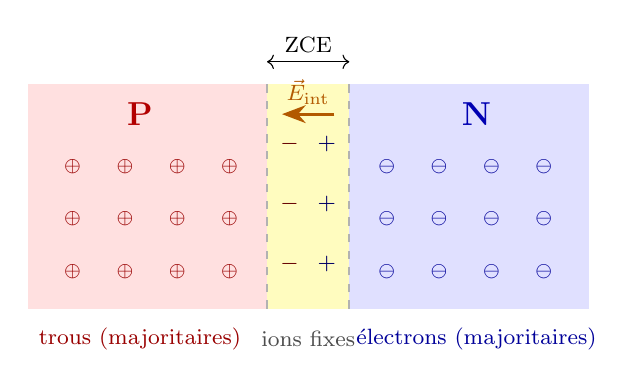
\begin{tikzpicture}[scale=0.95]
  % Régions P et N
  \fill[red!12] (0,0) rectangle (3.2,3);
  \fill[blue!12] (4.3,0) rectangle (7.5,3);
  \node[font=\bfseries\large, red!70!black] at (1.5,2.6) {P};
  \node[font=\bfseries\large, blue!70!black] at (6,2.6) {N};
  
  % Zone de déplétion
  \fill[yellow!25] (3.2,0) rectangle (4.3,3);
  \draw[dashed, thick, gray!60] (3.2,0) -- (3.2,3);
  \draw[dashed, thick, gray!60] (4.3,0) -- (4.3,3);
  
  % Label ZCE au-dessus (pas dans la zone)
  \draw[<->] (3.2,3.3) -- (4.3,3.3);
  \node[font=\footnotesize, above] at (3.75,3.3) {ZCE};
  
  % Porteurs majoritaires (espacés, hors ZCE)
  \foreach \x in {0.6, 1.3, 2.0, 2.7} {
    \foreach \y in {0.5, 1.2, 1.9} {
      \node[red!60!black, font=\scriptsize] at (\x,\y) {$\oplus$};
    }
  }
  \foreach \x in {4.8, 5.5, 6.2, 6.9} {
    \foreach \y in {0.5, 1.2, 1.9} {
      \node[blue!60!black, font=\scriptsize] at (\x,\y) {$\ominus$};
    }
  }
  
  % Ions fixes dans la ZCE (bien espacés)
  \foreach \y in {0.6, 1.4, 2.2} {
    \node[red!40!black, font=\footnotesize\bfseries] at (3.5,\y) {$-$};
    \node[blue!40!black, font=\footnotesize\bfseries] at (4.0,\y) {$+$};
  }
  
  % Champ électrique interne (au-dessus des ions, sous le label P/N)
  \draw[-{Stealth[length=3mm]}, very thick, orange!70!black] (4.1,2.6) -- (3.4,2.6);
  \node[orange!70!black, font=\footnotesize] at (3.75,2.9) {$\vec{E}_{\text{int}}$};
  
  % Légendes en dessous, bien espacées
  \node[font=\footnotesize, red!60!black] at (1.5,-0.4) {trous (majoritaires)};
  \node[font=\footnotesize, blue!60!black] at (6,-0.4) {électrons (majoritaires)};
  \node[font=\footnotesize, gray!60!black] at (3.75,-0.4) {ions fixes};
\end{tikzpicture}
\end{center}

\textbf{Mécanisme :} les électrons du côté N diffusent vers le P (où ils sont rares), et les trous du P diffusent vers le N. À l'interface, ils se \textbf{recombinent} et disparaissent, laissant derrière eux des \textbf{ions fixes} : ions négatifs côté P (bore ionisé), ions positifs côté N (phosphore ionisé). Ces ions créent un \textbf{champ électrique interne} $\vec{E}$ dirigé de N vers P, qui s'oppose à la diffusion et finit par l'arrêter. L'équilibre est atteint quand le courant de diffusion est exactement compensé par le courant de dérive (dû au champ).

\subsubsection*{Polarisation directe et inverse}

\begin{center}
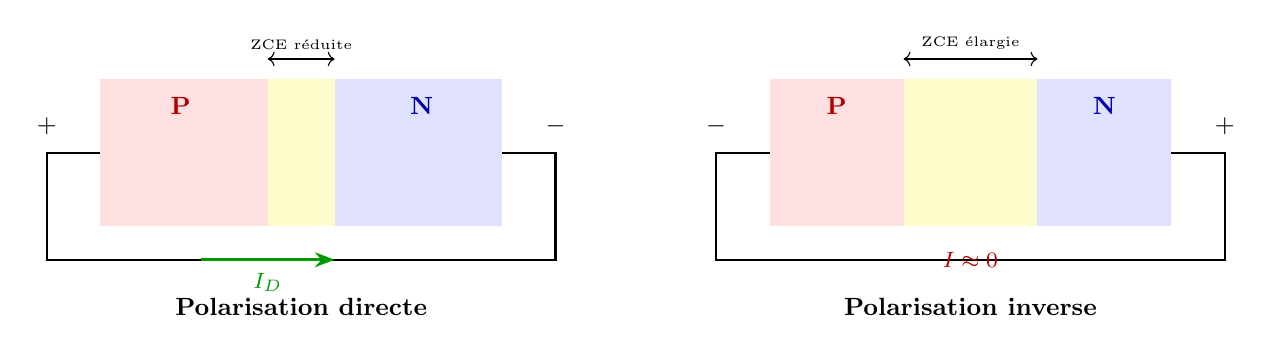
\begin{tikzpicture}[scale=0.85]
  % DIRECTE
  \begin{scope}[shift={(0,0)}]
    \fill[red!12] (0,0) rectangle (2.5,2.2);
    \fill[blue!12] (3.5,0) rectangle (6,2.2);
    \fill[yellow!20] (2.5,0) rectangle (3.5,2.2);
    \node[font=\small\bfseries, red!70!black] at (1.2,1.8) {P};
    \node[font=\small\bfseries, blue!70!black] at (4.8,1.8) {N};
    
    % ZCE label au-dessus
    \draw[<->] (2.5,2.5) -- (3.5,2.5);
    \node[font=\tiny, above] at (3,2.5) {ZCE réduite};
    
    % Fils de connexion + batterie
    \draw[thick] (0,1.1) -- (-0.8,1.1) -- (-0.8,-0.5) -- (6.8,-0.5) -- (6.8,1.1) -- (6,1.1);
    \node[font=\small] at (-0.8,1.5) {$+$};
    \node[font=\small] at (6.8,1.5) {$-$};
    
    % Courant SUR le fil du bas
    \draw[-{Stealth[length=2.5mm]}, very thick, green!60!black] (1.5,-0.5) -- (3.5,-0.5);
    \node[green!60!black, font=\footnotesize, below] at (2.5,-0.55) {$I_D$};
    
    \node[font=\small\bfseries] at (3,-1.2) {Polarisation directe};
  \end{scope}
  
  % INVERSE
  \begin{scope}[shift={(10,0)}]
    \fill[red!12] (0,0) rectangle (2,2.2);
    \fill[blue!12] (4,0) rectangle (6,2.2);
    \fill[yellow!20] (2,0) rectangle (4,2.2);
    \node[font=\small\bfseries, red!70!black] at (1,1.8) {P};
    \node[font=\small\bfseries, blue!70!black] at (5,1.8) {N};
    
    % ZCE label au-dessus
    \draw[<->] (2,2.5) -- (4,2.5);
    \node[font=\tiny, above] at (3,2.5) {ZCE élargie};
    
    % Fils de connexion + batterie inversée
    \draw[thick] (0,1.1) -- (-0.8,1.1) -- (-0.8,-0.5) -- (6.8,-0.5) -- (6.8,1.1) -- (6,1.1);
    \node[font=\small] at (-0.8,1.5) {$-$};
    \node[font=\small] at (6.8,1.5) {$+$};
    
    % Pas de courant
    \node[red!70!black, font=\footnotesize] at (3,-0.5) {$I \approx 0$};
    
    \node[font=\small\bfseries] at (3,-1.2) {Polarisation inverse};
  \end{scope}
\end{tikzpicture}
\end{center}

\begin{formule}
\textbf{Résumé physique :}
\begin{itemize}[nosep]
\item La \textbf{barrière de potentiel} intrinsèque ($V_0 \approx \SI{0.7}{V}$ pour le Si) est due au champ électrique interne de la ZCE.
\item \textbf{En direct} ($V_D > 0$) : la tension externe \textit{s'oppose} au champ interne $\Rightarrow$ la ZCE se \textit{rétrécit} $\Rightarrow$ les porteurs traversent $\Rightarrow$ courant. Quand $V_D \approx V_0$, la barrière est presque annulée et le courant croît exponentiellement.
\item \textbf{En inverse} ($V_D < 0$) : la tension externe \textit{renforce} le champ interne $\Rightarrow$ la ZCE s'\textit{élargit} $\Rightarrow$ aucun porteur majoritaire ne traverse. Seuls les porteurs \textit{minoritaires} (rares, d'origine thermique) créent le courant de fuite $I_S$.
\end{itemize}
\end{formule}

\begin{attention}
\textbf{Effet de la température :} $I_S$ double environ tous les \SI{10}{°C}. À \SI{25}{°C}, $I_S \sim \SI{1}{nA}$ pour une diode Si. À \SI{125}{°C}, $I_S \sim \SI{1}{\micro A}$. C'est pourquoi les circuits à diodes se comportent différemment à chaud : la tension de seuil $V_F$ \textit{diminue} d'environ $\SI{-2}{mV/°C}$. Ce coefficient est exploité dans les \textbf{capteurs de température à diode} et les \textbf{références de tension bandgap}.
\end{attention}

\subsection{L'équation de Shockley}

La relation $I(V)$ exacte d'une diode est donnée par l'\textbf{équation de Shockley} :

\begin{formule}
\[
\boxed{I_D = I_S\left(e^{V_D / nV_T} - 1\right)}
\]
\begin{itemize}[nosep]
\item $I_S$ : courant de saturation inverse ($\sim\SI{1}{nA}$ à \SI{1}{\micro A} selon la diode et la température).
\item $V_T = kT/q$ : \textbf{tension thermique} ($\SI{26}{mV}$ à \SI{25}{°C}).
\item $n$ : facteur d'idéalité ($1$ à $2$, typiquement $\approx 1$ pour les diodes Si standard).
\item $k = \SI{1.381e-23}{J/K}$ : constante de Boltzmann.
\item $q = \SI{1.602e-19}{C}$ : charge de l'électron.
\item $T$ : température absolue (K).
\end{itemize}
\end{formule}

\begin{intuition}
\textbf{Ce que dit Shockley :} le courant croît \textit{exponentiellement} avec la tension. Un changement de seulement $\SI{60}{mV}$ (à $n = 1$) multiplie le courant par \textbf{10}. C'est pourquoi la caractéristique directe semble ``verticale'' à l'échelle du circuit : entre \SI{0.6}{V} (quasi pas de courant) et \SI{0.7}{V} (courant nominal), il n'y a que \SI{100}{mV} de différence, mais le courant a changé de plusieurs décades.
\end{intuition}

\subsection{Résistance dynamique}

Au voisinage d'un point de fonctionnement $(V_D, I_D)$, la diode se comporte comme une petite résistance :

\begin{formule}
\[
\boxed{r_d = \frac{\mathrm{d}V_D}{\mathrm{d}I_D} = \frac{nV_T}{I_D}}
\]
À $I_D = \SI{1}{mA}$ ($n = 1$) : $r_d = 26/1 = \SI{26}{\ohm}$.

À $I_D = \SI{10}{mA}$ : $r_d = \SI{2.6}{\ohm}$.
\end{formule}

Cette résistance dynamique est utilisée dans le modèle petit signal (circuits analogiques) et explique pourquoi la chute de tension ``augmente un peu'' quand le courant augmente.

\subsection{Redressement simple alternance}

La première application historique de la diode : convertir l'AC en DC.

\begin{center}
\begin{circuitikz}[scale=0.85]
  \draw (0,0) to[sinusoidal voltage source, l=$v_{\text{AC}}$] (0,2.5)
        to[D, l=$D$] (3,2.5)
        to[R, l=$R$] (3,0) -- (0,0);
\end{circuitikz}
\end{center}

La diode ne conduit que pendant les alternances positives. La tension aux bornes de $R$ est une succession de demi-sinusoïdes :

\begin{itemize}[nosep]
\item Alternance positive : $v_{\text{out}} = v_{\text{AC}} - V_F$ (la diode conduit).
\item Alternance négative : $v_{\text{out}} = 0$ (la diode est bloquée).
\end{itemize}

La tension moyenne en sortie est : $V_{\text{moy}} = (\hat{V} - V_F)/\pi \approx \hat{V}/\pi$.

\subsection{Pont de Graetz (redressement double alternance)}

Pour utiliser les \textit{deux} alternances, on utilise un pont de 4 diodes :

\begin{center}
\begin{circuitikz}[scale=0.9]
  % AC source à gauche
  \draw (0,0) to[sinusoidal voltage source, l=$v_{\text{AC}}$] (0,4);
  
  % Fil haut : de la source au noeud gauche-haut
  \draw (0,4) -- (2,4);
  % Fil bas : de la source au noeud gauche-bas
  \draw (0,0) -- (2,0);
  
  % Branche gauche du pont
  \draw (2,4) to[D, l=$D_1$] (2,2);    % D1 : haut vers milieu
  \draw (2,2) to[D, l=$D_3$] (2,0);    % D3 : milieu vers bas
  
  % Branche droite du pont
  \draw (5,4) to[D, l=$D_2$] (5,2);    % D2 : haut vers milieu
  \draw (5,2) to[D, l=$D_4$] (5,0);    % D4 : milieu vers bas
  
  % Fil haut reliant les deux branches
  \draw (2,4) -- (5,4);
  % Fil bas reliant les deux branches
  \draw (2,0) -- (5,0);
  
  % Sortie DC : noeud milieu-gauche (2,2) = -, noeud milieu-droit (5,2) = +
  % On sort par le haut du pont (noeud commun D1-D2 côté cathode)
  \draw (5,4) -- (7,4);
  \draw (2,0) -- (7,0);
  
  % Charge
  \draw (7,4) to[R, l=$R_L$] (7,0);
  
  % Labels DC
  \node[font=\small] at (7.5,3.8) {$+$};
  \node[font=\small] at (7.5,0.2) {$-$};
  \node[font=\small, right] at (7.3,2) {$V_{\text{out}}$};
  
  % Noeuds
  \filldraw (2,4) circle (1.5pt);
  \filldraw (2,0) circle (1.5pt);
  \filldraw (5,4) circle (1.5pt);
  \filldraw (5,0) circle (1.5pt);
\end{circuitikz}
\end{center}

Les deux alternances sont redressées. La tension moyenne est : $V_{\text{moy}} = 2(\hat{V} - 2V_F)/\pi$.

\begin{attention}
Le pont de diodes perd \textbf{deux chutes de diode} ($2V_F \approx \SI{1.4}{V}$ en Si). Pour les alimentations basse tension ($\SI{3.3}{V}$, $\SI{5}{V}$), c'est une perte significative. On utilise alors des \textbf{diodes Schottky} ($2 \times \SI{0.3}{V} = \SI{0.6}{V}$) ou un \textbf{redressement synchrone} (MOSFETs, perte $< \SI{0.1}{V}$).
\end{attention}

\subsection{Les variantes de diodes}

\begin{center}
\renewcommand{\arraystretch}{1.4}
\begin{tabular}{p{2.5cm}p{2cm}p{7cm}}
\toprule
\textbf{Type} & \textbf{$V_F$ / $V_{BR}$} & \textbf{Fonction et usage} \\
\midrule
\textbf{Redressement} (1N400x) & $\SI{0.7}{V}$ & Redressement secteur, protection. Lente ($t_{rr} \sim \SI{30}{\micro s}$). \\
\textbf{Schottky} & $\SI{0.2}{V}$--$\SI{0.4}{V}$ & Redressement rapide, convertisseurs DC-DC. $V_{BR}$ limité ($< \SI{100}{V}$). \\
\textbf{Zener} & $V_Z$ choisi & Régulation de tension (fonctionne en inverse). De \SI{2.4}{V} à \SI{200}{V}. \\
\textbf{LED} & $\SI{1.8}{V}$--$\SI{3.5}{V}$ & Signalisation, éclairage. Émet de la lumière en direct. \\
\textbf{TVS} & $V_{BR}$ choisi & Protection contre les surtensions (ESD, foudre). Très rapide ($< \SI{1}{ns}$). \\
\textbf{Varicap} & — & Capacité variable commandée en tension. Utilisée dans les VCO et les PLL. \\
\textbf{Photodiode} & — & Génère un courant proportionnel à la lumière reçue. Capteurs, fibres optiques. \\
\bottomrule
\end{tabular}
\end{center}

% ----------------------------------------------------------------------------
\section{Niveau Ingénieur}

\begin{ingenieur}
Modèle SPICE, effets dynamiques, pertes de commutation, et diode dans les convertisseurs de puissance.
\end{ingenieur}

\subsection{Modèle SPICE de la diode}

Le simulateur SPICE utilise un modèle beaucoup plus complet que Shockley. Les paramètres principaux :

\begin{center}
\begin{tabular}{llll}
\toprule
\textbf{Paramètre} & \textbf{Symbole} & \textbf{Typique (1N4148)} & \textbf{Signification} \\
\midrule
Courant de saturation & $I_S$ & \SI{2.52}{nA} & Fuite inverse \\
Facteur d'idéalité & $n$ (N) & $1{,}75$ & Pente exponentielle \\
Résistance série & $R_S$ & \SI{0.568}{\ohm} & Résistance du bulk Si \\
Tension de claquage & $BV$ & \SI{100}{V} & Tension inverse max \\
Capacité de jonction & $C_{J0}$ & \SI{4}{pF} & Capacité à $V = 0$ \\
Temps de recouvrement & $T_T$ & \SI{11.5}{ns} & Temps de transit \\
\bottomrule
\end{tabular}
\end{center}

\subsection{Capacité de jonction et comportement dynamique}

La zone de déplétion se comporte comme un \textbf{condensateur} dont la capacité varie avec la tension inverse :

\begin{formule}
\[
C_j(V) = \frac{C_{J0}}{(1 - V/V_J)^M}
\]
avec $V_J \approx \SI{0.7}{V}$ (potentiel de jonction) et $M \approx 0{,}33$ à $0{,}5$.
\end{formule}

\begin{pratique}
\textbf{Conséquences :}
\begin{itemize}[nosep]
\item \textbf{Varicap :} cette dépendance est exploitée volontairement. En faisant varier la tension inverse, on change la capacité. C'est le principe des oscillateurs commandés en tension (VCO).
\item \textbf{Limitation en fréquence :} pour une diode de redressement, $C_j$ limite la vitesse de commutation. Une 1N4007 ($C_j \sim \SI{15}{pF}$, $t_{rr} \sim \SI{30}{\micro s}$) est inutilisable au-dessus de $\sim\SI{10}{kHz}$. Une Schottky ($t_{rr} < \SI{10}{ns}$) monte à des dizaines de MHz.
\end{itemize}
\end{pratique}

\subsection{Temps de recouvrement inverse ($t_{rr}$)}

Quand une diode passe de l'état passant à l'état bloqué, elle ne se bloque pas instantanément. Pendant un bref instant ($t_{rr}$), un \textbf{courant inverse} circule (évacuation des charges stockées dans la jonction).

\begin{attention}
\textbf{En commutation de puissance, $t_{rr}$ est critique.} Pendant le recouvrement, la diode dissipe de la puissance ($V_R \times I_{rr}$). À haute fréquence de commutation (\SI{100}{kHz}--\SI{1}{MHz} dans les convertisseurs modernes), ces pertes de commutation peuvent devenir dominantes.

\textbf{Solutions :}
\begin{itemize}[nosep]
\item Diodes Schottky : pas de recouvrement (jonction métal-semi-conducteur, pas de charges stockées).
\item Diodes ultrafast ($t_{rr} < \SI{50}{ns}$) : compromis pour les applications moyenne fréquence.
\item Redressement synchrone (MOSFET) : élimine complètement le problème.
\end{itemize}
\end{attention}

\subsection{Pertes dans une diode de puissance}

Les pertes totales dans une diode ont deux composantes :

\begin{formule}
\[
\boxed{P_{\text{total}} = \underbrace{V_F \cdot I_{\text{moy}}}_{\text{pertes en conduction}} + \underbrace{f_{\text{sw}} \cdot E_{\text{rr}}}_{\text{pertes de commutation}}}
\]
\begin{itemize}[nosep]
\item $V_F \cdot I_{\text{moy}}$ : pertes ``statiques'' dues à la chute directe.
\item $f_{\text{sw}} \cdot E_{\text{rr}}$ : pertes ``dynamiques'' dues au recouvrement inverse à chaque commutation. $E_{\text{rr}}$ est l'énergie dissipée par événement de recouvrement.
\end{itemize}
\end{formule}

\begin{pratique}
\textbf{Exemple :} diode 1N5819 (Schottky, $V_F = \SI{0.45}{V}$) dans un convertisseur buck à $f_{\text{sw}} = \SI{500}{kHz}$, $I_{\text{moy}} = \SI{1}{A}$ :

Pertes conduction : $0{,}45 \times 1 = \SI{0.45}{W}$.

Pertes commutation : quasi nulles (Schottky, pas de $t_{rr}$). $P_{\text{total}} \approx \SI{0.45}{W}$.

Comparaison avec une 1N4007 ($V_F = \SI{0.9}{V}$, $t_{rr} = \SI{30}{\micro s}$) : pertes conduction $= \SI{0.9}{W}$, pertes commutation $\gg \SI{1}{W}$ à \SI{500}{kHz}. \textbf{Totalement inadaptée.}
\end{pratique}

\subsection{La diode Zener : régulation de tension}

La diode Zener est conçue pour fonctionner en \textbf{claquage inverse contrôlé}. Contrairement à une diode classique (où le claquage est destructeur), la Zener est fabriquée pour supporter un courant inverse stable. Elle maintient une tension quasi constante $V_Z$ à ses bornes.

\textbf{Circuit de régulation Zener :}

\begin{center}
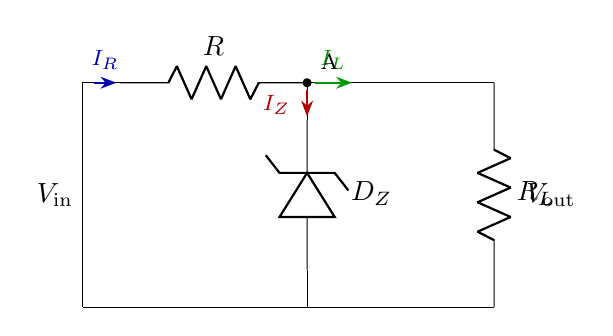
\begin{tikzpicture}[scale=0.95]
  % Circuit principal
  \draw (0,0) -- (0,3) -- (0.5,3);
  \draw (0.5,3) to[R, l=$R$] (3,3);
  \draw (3,3) -- (3,2.5);
  \draw (3,2.5) to[zzD, l=$D_Z$, invert] (3,0.5);
  \draw (3,0.5) -- (3,0) -- (0,0);
  
  % Charge
  \draw (3,3) -- (5.5,3);
  \draw (5.5,3) to[R, l=$R_L$] (5.5,0);
  \draw (5.5,0) -- (3,0);
  
  % Labels tension
  \node[left] at (0,1.5) {$V_{\text{in}}$};
  \node[right] at (5.8,1.5) {$V_{\text{out}}$};
  
  % Courant I_R sur le fil AVANT R (entre source et R)
  \draw[-{Stealth[length=2mm]}, blue!70!black, thick] (0.15,3) -- (0.45,3);
  \node[blue!70!black, above, font=\footnotesize] at (0.3,3.05) {$I_R$};
  
  % Courant I_Z sur le fil vertical ENTRE jonction et Zener
  \draw[-{Stealth[length=2mm]}, red!70!black, thick] (3,2.9) -- (3,2.55);
  \node[red!70!black, left, font=\footnotesize] at (2.9,2.7) {$I_Z$};
  
  % Courant I_L sur le fil horizontal VERS la charge
  \draw[-{Stealth[length=2mm]}, green!60!black, thick] (3.1,3) -- (3.6,3);
  \node[green!60!black, above, font=\footnotesize] at (3.35,3.05) {$I_L$};
  
  % Noeud A
  \filldraw (3,3) circle (1.5pt);
  \node[above right, font=\footnotesize] at (3.05,3.05) {A};
\end{tikzpicture}
\end{center}

\begin{formule}
\textbf{Principe :} la résistance $R$ limite le courant total. La Zener ``absorbe'' l'excédent de courant que la charge ne consomme pas, maintenant ainsi $V_{\text{out}} = V_Z$ constant.

\textbf{Loi des n\oe uds au point A :} $I_R = I_Z + I_L$

\textbf{Courant dans $R$ :} $I_R = \dfrac{V_{\text{in}} - V_Z}{R}$

\textbf{Courant dans la Zener :} $\boxed{I_Z = \frac{V_{\text{in}} - V_Z}{R} - I_L}$

\textbf{Conditions de fonctionnement :}
\begin{itemize}[nosep]
\item $I_Z > I_{Z,\min}$ ($\sim\SI{1}{mA}$ à \SI{5}{mA}) : la Zener doit avoir assez de courant pour rester en claquage.
\item $I_Z < I_{Z,\max}$ : sinon la puissance dissipée dépasse $P_{\max}$ et la Zener grille.
\item Si $I_Z < 0$ : la Zener ne conduit plus, \textbf{elle ne régule plus}. La tension de sortie chute.
\end{itemize}
\end{formule}

\begin{pratique}
\textbf{Méthode de résolution d'un circuit à Zener (hypothèse/vérification) :}

La méthode rigoureuse est identique à celle des circuits à diode :
\begin{enumerate}[nosep]
\item \textbf{Hypothèse :} on suppose que la Zener conduit ($V_{\text{out}} = V_Z$).
\item \textbf{Calcul :} on calcule $I_R$, $I_L$, puis $I_Z = I_R - I_L$.
\item \textbf{Vérification :} si $I_Z > 0$, l'hypothèse est correcte. Si $I_Z < 0$, l'hypothèse est fausse : la Zener est bloquée, et il faut recalculer avec un simple diviseur résistif (Zener = circuit ouvert).
\end{enumerate}
\end{pratique}

\begin{attention}
\textbf{Limites de la régulation Zener :}
\begin{itemize}[nosep]
\item \textbf{Rendement catastrophique} : toute la puissance excédentaire est dissipée dans $R$ et la Zener.
\item \textbf{Régulation imparfaite} : la tension $V_Z$ n'est pas parfaitement constante --- elle varie légèrement avec $I_Z$ (résistance dynamique $r_Z \sim \SI{1}{\ohm}$ à \SI{50}{\ohm}).
\item \textbf{Dérive en température} : les Zener de basse tension ($V_Z < \SI{5}{V}$, effet Zener pur) ont un coefficient négatif ; les hautes tensions ($V_Z > \SI{6}{V}$, effet avalanche) ont un coefficient positif. À $V_Z \approx \SI{5.6}{V}$, les deux effets se compensent $\Rightarrow$ dérive minimale. C'est pourquoi les références de tension Zener sont souvent à \SI{5.6}{V}.
\end{itemize}
En pratique, la régulation Zener n'est utilisée que pour les \textbf{faibles courants} ($< \SI{50}{mA}$), comme référence de tension, ou comme protection (écrêtage). Pour les courants plus élevés, on utilise un \textbf{régulateur intégré} (LDO ou DC-DC).
\end{attention}

% === EXERCICES DU CHAPITRE 15 ===
\section*{Exercices}
\addcontentsline{toc}{section}{Exercices}

\subsection*{Niveau débutant}

\textbf{Exercice 15.1 ---} Une LED rouge ($V_F = \SI{1.8}{V}$, $I = \SI{15}{mA}$) doit être alimentée par une batterie de \SI{9}{V}. Quelle résistance de limitation utiliser ? Quelle puissance dissipe-t-elle ?

\begin{pratique}
\textbf{Solution :} $R = (V_{\text{bat}} - V_F)/I = (9 - 1{,}8)/0{,}015 = \SI{480}{\ohm}$ $\to$ \SI{470}{\ohm} (E24).

$P_R = (V_{\text{bat}} - V_F) \times I = 7{,}2 \times 0{,}015 = \SI{108}{mW}$. Une résistance 1/4\,W suffit.

$P_{\text{LED}} = V_F \times I = 1{,}8 \times 0{,}015 = \SI{27}{mW}$.
\end{pratique}

\textbf{Exercice 15.2 ---} Un circuit est alimenté par $E = \SI{12}{V}$ via une diode de protection (Si, $V_F = \SI{0.7}{V}$). Quelle tension arrive effectivement au circuit ? Si le circuit consomme \SI{200}{mA}, quelle puissance la diode dissipe-t-elle ?

\begin{pratique}
\textbf{Solution :} $V_{\text{circuit}} = E - V_F = 12 - 0{,}7 = \SI{11.3}{V}$.

$P_D = V_F \times I = 0{,}7 \times 0{,}2 = \SI{140}{mW}$.

Pour réduire la perte, on peut utiliser une Schottky ($V_F \approx \SI{0.3}{V}$, $P = \SI{60}{mW}$) ou un MOSFET de protection (``ideal diode'', $V_F < \SI{50}{mV}$).
\end{pratique}

\subsection*{Niveau intermédiaire}

\textbf{Exercice 15.3 ---} Un pont de Graetz (4 diodes Si) redresse le secteur (\SI{230}{V} eff, \SI{50}{Hz}) pour alimenter un condensateur de filtrage de \SI{470}{\micro F}. Calculez la tension crête en sortie, la tension d'ondulation (ripple) pour une charge tirant \SI{0.5}{A}, et la puissance dissipée dans les diodes.

\begin{pratique}
\textbf{Solution :} Tension crête : $\hat{V} = 230\sqrt{2} - 2V_F = 325 - 1{,}4 = \SI{323.6}{V}$.

Ondulation (approximation classique pour charge résistive) : $\Delta V \approx I/(fC) = 0{,}5/(100\times470\times10^{-6}) = \SI{10.6}{V}$ (à $f = 2\times\SI{50}{Hz}$, car double alternance).

$\Delta V / \hat{V} = 10{,}6/323{,}6 = 3{,}3\%$. Acceptable pour une alimentation avec régulateur en aval.

Puissance diodes : $P = 2V_F \times I = 1{,}4 \times 0{,}5 = \SI{0.7}{W}$ (deux diodes conduisent à chaque instant).
\end{pratique}

\textbf{Exercice 15.4 ---} À $I_D = \SI{1}{mA}$, une diode Si a $V_D = \SI{0.65}{V}$. À $I_D = \SI{10}{mA}$, $V_D = \SI{0.72}{V}$. Vérifiez la cohérence avec l'équation de Shockley et estimez $n$.

\begin{pratique}
\textbf{Solution :} De Shockley : $V_D = nV_T \ln(I_D/I_S)$ (en négligeant le $-1$).

$\Delta V = V_2 - V_1 = nV_T \ln(I_2/I_1) = nV_T \ln(10)$.

$0{,}72 - 0{,}65 = n \times 0{,}026 \times 2{,}303$.

$0{,}07 = n \times 0{,}0599 \Rightarrow n = 1{,}17$.

Cohérent : $n$ entre 1 et 2, typique d'une diode Si. On a aussi confirmé la règle : $\sim\SI{60}{mV}$ par décade de courant (pour $n \approx 1$).
\end{pratique}

\subsection*{Niveau ingénieur}

\textbf{Exercice 15.5 ---} Un convertisseur buck fonctionne à $f_{\text{sw}} = \SI{300}{kHz}$, $V_{\text{in}} = \SI{12}{V}$, $V_{\text{out}} = \SI{5}{V}$, $I_L = \SI{2}{A}$. Comparez les pertes totales entre une diode 1N5819 (Schottky, $V_F = \SI{0.45}{V}$, $t_{rr} \approx 0$) et une 1N4007 ($V_F = \SI{0.9}{V}$, $t_{rr} = \SI{30}{\micro s}$, $I_{rr} = \SI{0.5}{A}$).

\begin{pratique}
\textbf{Solution :}

\textbf{1N5819 (Schottky) :} duty cycle $D = V_{\text{out}}/V_{\text{in}} = 5/12 = 0{,}42$. La diode conduit pendant $(1-D) = 58\%$ du temps. $I_{\text{moy,diode}} = I_L(1-D) = 2\times0{,}58 = \SI{1.16}{A}$.

$P_{\text{cond}} = V_F \times I_{\text{moy}} = 0{,}45 \times 1{,}16 = \SI{0.52}{W}$.

$P_{\text{sw}} \approx 0$ (Schottky). $P_{\text{total}} \approx \SI{0.52}{W}$.

\textbf{1N4007 :} $P_{\text{cond}} = 0{,}9 \times 1{,}16 = \SI{1.04}{W}$.

$E_{rr} \approx \frac{1}{2}V_R \times I_{rr} \times t_{rr} = \frac{1}{2}\times12\times0{,}5\times30\times10^{-6} = \SI{90}{\micro J}$.

$P_{\text{sw}} = f \times E_{rr} = 300000\times90\times10^{-6} = \SI{27}{W}$ !!

$P_{\text{total}} \approx \SI{28}{W}$. La diode fond en quelques secondes. La 1N4007 est \textbf{totalement inadaptée} à la commutation HF.
\end{pratique}

\textbf{Exercice 15.6 ---} Une diode Zener de \SI{5.1}{V} est utilisée pour réguler une tension issue d'une alimentation variable ($V_{\text{in}} = \SI{8}{V}$ à \SI{15}{V}). $R = \SI{220}{\ohm}$. La charge consomme $I_L = \SI{10}{mA}$. Calculez le courant dans la Zener et la puissance dissipée pour $V_{\text{in}} = \SI{8}{V}$ et $V_{\text{in}} = \SI{15}{V}$. La Zener tient-elle ($P_{\max} = \SI{0.5}{W}$) ?

\begin{pratique}
\textbf{Solution :}

À $V_{\text{in}} = \SI{8}{V}$ : $I_R = (V_{\text{in}} - V_Z)/R = (8-5{,}1)/220 = \SI{13.2}{mA}$.

$I_Z = I_R - I_L = 13{,}2 - 10 = \SI{3.2}{mA}$. OK ($> 0$, la Zener régule).

$P_Z = V_Z \times I_Z = 5{,}1\times3{,}2 = \SI{16.3}{mW}$.

À $V_{\text{in}} = \SI{15}{V}$ : $I_R = (15-5{,}1)/220 = \SI{45}{mA}$.

$I_Z = 45 - 10 = \SI{35}{mA}$. $P_Z = 5{,}1\times35 = \SI{178.5}{mW}$. OK ($< \SI{500}{mW}$).

$P_R = (V_{\text{in}}-V_Z)^2/R = 9{,}9^2/220 = \SI{445}{mW}$. Il faut une résistance 1/2\,W.

\textbf{Rendement à $V_{\text{in}} = \SI{15}{V}$ :} $\eta = P_L/P_{\text{in}} = (5{,}1\times10)/(15\times45) = 51/675 = 7{,}6\%$.

C'est catastrophique : $92\%$ de la puissance est perdue ! Pour une charge de \SI{10}{mA}, c'est tolérable. Au-delà, il faut un régulateur intégré.
\end{pratique}

\textbf{Exercice 15.7 ---} (Méthode hypothèse/vérification) On reprend le circuit de l'exercice 15.6 ($V_Z = \SI{5.1}{V}$, $R = \SI{220}{\ohm}$) mais cette fois avec $V_{\text{in}} = \SI{6}{V}$ et $R_L = \SI{100}{\ohm}$.

(a) On \textit{suppose} que la Zener conduit. Calculez $I_R$, $I_L$, et $I_Z$. L'hypothèse est-elle vérifiée ?

(b) Si la Zener ne conduit pas, recalculez la tension de sortie réelle.

\begin{pratique}
\textbf{Solution :}

\textbf{(a) Hypothèse : la Zener conduit} $\Rightarrow V_{\text{out}} = V_Z = \SI{5.1}{V}$.

$I_R = (V_{\text{in}} - V_Z)/R = (6 - 5{,}1)/220 = 0{,}9/220 = \SI{4.09}{mA}$.

$I_L = V_Z/R_L = 5{,}1/100 = \SI{51}{mA}$.

$I_Z = I_R - I_L = 4{,}09 - 51 = \SI{-46.9}{mA}$.

$I_Z < 0$ ! \textbf{L'hypothèse est FAUSSE.} La Zener ne peut pas ``absorber'' un courant négatif (elle n'est pas une source de courant). Physiquement, la charge demande beaucoup plus de courant ($\SI{51}{mA}$) que ce que $R$ peut fournir ($\SI{4}{mA}$).

\textbf{(b) La Zener est bloquée} $\Rightarrow$ on la remplace par un circuit ouvert. Le circuit devient un simple diviseur $R$ -- $R_L$ :

$V_{\text{out}} = V_{\text{in}} \times \dfrac{R_L}{R + R_L} = 6 \times \dfrac{100}{220 + 100} = 6 \times \dfrac{100}{320} = \SI{1.875}{V}$.

La tension de sortie n'est que \SI{1.875}{V} --- bien en dessous de $V_Z$. La Zener ne régule pas du tout : la charge est trop gourmande pour la valeur de $R$ choisie.

\textbf{Pour que ça fonctionne :} il faudrait $I_R > I_L$, donc $(V_{\text{in}}-V_Z)/R > V_Z/R_L$. Avec $R_L = \SI{100}{\ohm}$ et $V_Z = \SI{5.1}{V}$ : $I_L = \SI{51}{mA}$. Il faudrait $R < (V_{\text{in}}-V_Z)/I_L = 0{,}9/0{,}051 = \SI{17.6}{\ohm}$. Mais alors la puissance dissipée dans $R$ serait $(6-5{,}1)^2/17{,}6 = \SI{46}{mW}$ et la Zener consommerait presque rien --- c'est un cas limite très peu pratique.

\textbf{Morale :} la régulation Zener ne fonctionne que si $I_L \ll I_R$. Pour des charges qui consomment beaucoup, \textbf{il faut un régulateur actif}.
\end{pratique}

\subsection*{Questions de compréhension}

\begin{enumerate}[nosep]
\item Pourquoi une diode a-t-elle une tension de seuil $V_F \neq 0$ ? Répondez en termes de barrière de potentiel de la jonction PN.
\item On branche deux diodes en parallèle pour ``partager le courant''. Est-ce une bonne idée ? Pourquoi ? (Pensez à l'exponentielle et aux tolérances sur $V_F$.)
\item Pourquoi les diodes Schottky ont-elles un $V_F$ plus bas que les diodes Si ? Quel est le compromis ?
\item Une LED est-elle une diode ? Si oui, pourquoi émet-elle de la lumière alors qu'une diode Si ordinaire n'en émet pas ?
\end{enumerate}

% === RÉSUMÉ DU CHAPITRE 15 ===
\section*{Résumé du chapitre}
\addcontentsline{toc}{section}{Résumé du chapitre}

\begin{bases}[title={\color{white} Résumé --- Les Bases}]
\begin{center}
\renewcommand{\arraystretch}{1.3}
\begin{tabular}{p{4cm}p{9cm}}
\toprule
Principe & Conduit en direct (A$\to$K), bloque en inverse \\
Seuil & $V_F \approx \SI{0.7}{V}$ (Si), $\SI{0.3}{V}$ (Schottky), $\SI{1.8}{V}$+ (LED) \\
Modèle pratique & $V_D = V_F$ en direct, $I_D = 0$ en inverse \\
Résistance série & Toujours limiter le courant ! \\
\bottomrule
\end{tabular}
\end{center}
\end{bases}

\begin{approfondissement}[title={\color{white} Résumé --- Approfondissement}]
\begin{center}
\renewcommand{\arraystretch}{1.3}
\begin{tabular}{p{4cm}p{9cm}}
\toprule
Jonction PN & Zone de déplétion = barrière de $\sim\SI{0.7}{V}$ \\
Shockley & $I = I_S(e^{V/nV_T}-1)$ --- exponentielle, $\SI{60}{mV/décade}$ \\
$r_d$ & $nV_T/I_D$ --- résistance dynamique petit signal \\
Redressement & Simple alternance, pont de Graetz + filtrage \\
Variantes & Schottky, Zener, LED, TVS, varicap, photodiode \\
\bottomrule
\end{tabular}
\end{center}
\end{approfondissement}

\begin{ingenieur}[title={\color{white} Résumé --- Niveau Ingénieur}]
\begin{center}
\renewcommand{\arraystretch}{1.3}
\begin{tabular}{p{4cm}p{9cm}}
\toprule
Modèle SPICE & $I_S$, $n$, $R_S$, $C_{J0}$, $BV$, $T_T$ \\
$C_j(V)$ & Capacité variable $\Rightarrow$ varicap (VCO), limite en fréquence \\
$t_{rr}$ & Recouvrement inverse --- pertes de commutation à HF \\
Pertes totales & $P = V_F I_{\text{moy}} + f_{\text{sw}} E_{rr}$ --- Schottky élimine $E_{rr}$ \\
\bottomrule
\end{tabular}
\end{center}
\end{ingenieur}

% ============================================================================
% CHAPITRE 16 : LE TRANSISTOR BIPOLAIRE (BJT)
% ============================================================================

% ============================================================================
% CHAPITRE 16 : LE TRANSISTOR BIPOLAIRE (BJT) — VERSION PEER-REVIEW
% ============================================================================
% ============================================================================
% CHAPITRE 16 : LE TRANSISTOR BIPOLAIRE (BJT)
% VERSION RÉVISÉE — niveau peer-review
% Fichier autonome à intégrer dans Bible_Elec.tex
% ============================================================================

\chapter{Le Transistor Bipolaire (BJT)}

\begin{center}
\textit{Le transistor bipolaire est le premier composant actif\\
à semi-conducteurs de l'histoire (1947, Bardeen, Brattain, Shockley).\\
Son principe : une tension base-émetteur contrôle l'injection\\
de porteurs à travers une base mince, créant un courant collecteur\\
bien supérieur au courant de commande.}
\end{center}

\vspace{0.5cm}

Contrairement à une idée reçue tenace, le BJT n'est \textbf{pas} fondamentalement ``commandé en courant''. C'est la \textit{tension} $V_{BE}$ qui contrôle physiquement le courant $I_C$ via l'injection de porteurs dans la base. Le courant de base $I_B$ est une \textit{conséquence} des recombinaisons dans la base, pas la cause du courant collecteur. Cette distinction, qui peut sembler académique, est en réalité cruciale pour comprendre la transconductance, le bruit, et la conception des circuits intégrés analogiques.

Ce chapitre présente le BJT selon trois niveaux de lecture : l'intuition (analogies et règles pratiques), le modèle ingénieur (outils de calcul), et le modèle physique (transport de porteurs et champs).

% ============================================================================
\section{Les Bases}

\begin{bases}
Niveau intuitif : fonctionnement qualitatif, règles pratiques, commutation. Prérequis : chapitres 1 à 3 et chapitre 15 (diode, jonction PN).
\end{bases}

\subsection{Un composant à trois bornes}

Un transistor bipolaire (BJT, \textit{Bipolar Junction Transistor}) possède \textbf{trois bornes} :

\begin{itemize}[nosep]
\item \textbf{Base} (B) : la borne de commande.
\item \textbf{Collecteur} (C) : la borne par laquelle entre le courant principal.
\item \textbf{Émetteur} (E) : la borne par laquelle sort le courant total.
\end{itemize}

\begin{center}
\begin{circuitikz}[scale=1.0, american]
  % NPN
  \begin{scope}[shift={(0,0)}]
    \draw (0,0) node[npn](Q1){};
    \draw (Q1.B) -- ++(-0.5,0) node[left, font=\small]{B};
    \draw (Q1.C) -- ++(0,0.5) node[above, font=\small]{C};
    \draw (Q1.E) -- ++(0,-0.5) node[below, font=\small]{E};
    \node[font=\bfseries] at (0,-2.2) {NPN};
  \end{scope}
  % PNP
  \begin{scope}[shift={(5,0)}]
    \draw (0,0) node[pnp](Q2){};
    \draw (Q2.B) -- ++(-0.5,0) node[left, font=\small]{B};
    \draw (Q2.E) -- ++(0,0.5) node[above, font=\small]{E};
    \draw (Q2.C) -- ++(0,-0.5) node[below, font=\small]{C};
    \node[font=\bfseries] at (0,-2.2) {PNP};
  \end{scope}
\end{circuitikz}
\end{center}

La flèche sur l'émetteur indique le sens du courant \textit{conventionnel}. Ce chapitre traite principalement du \textbf{NPN}, le plus courant (2N2222, BC547, 2N3904). Le PNP fonctionne de manière symétrique avec tensions et courants inversés.

\subsection{Le principe : une tension contrôle un courant}

\begin{analogie}
\textbf{Le robinet d'eau.} Imaginez un gros tuyau (collecteur $\to$ émetteur) avec un robinet commandé par la \textit{position} d'un levier (la tension $V_{BE}$) :
\begin{itemize}[nosep]
\item Levier en dessous du seuil : le robinet est fermé $\Rightarrow$ pas de débit. Transistor \textbf{bloqué}.
\item Levier légèrement au-dessus du seuil : un débit proportionnel à l'ouverture $\Rightarrow$ \textbf{régime actif} (amplification).
\item Levier grand ouvert : le débit est limité par le tuyau lui-même, pas par le robinet $\Rightarrow$ transistor \textbf{saturé}.
\end{itemize}
\textit{Tourner le levier demande un effort (le courant de base $I_B$), mais c'est la position du levier (la tension $V_{BE}$) qui détermine le débit.}
\end{analogie}

\begin{formule}
\textbf{Relation pratique (régime actif) :}
\[
\boxed{I_C \approx \beta \cdot I_B}
\]
\begin{itemize}[nosep]
\item $I_C$ : courant collecteur (le courant utile).
\item $I_B$ : courant de base (le courant de commande).
\item $\beta$ (ou $h_{FE}$) : gain en courant. Typiquement 50 à 500.
\end{itemize}
\end{formule}

\begin{attention}
\textbf{$\beta$ est un paramètre pratique, pas une constante physique.} Il varie fortement avec :
\begin{itemize}[nosep]
\item le courant $I_C$ (chute à faible et fort courant),
\item la tension $V_{CE}$ (effet Early),
\item la température (augmente d'environ $+0{,}5\%/°$C à $+1\%/°$C),
\item le lot de fabrication (dispersions de 1 à 5 entre $\beta_{\min}$ et $\beta_{\max}$).
\end{itemize}
\textbf{Conséquence :} on ne conçoit \textbf{jamais} un circuit dont le fonctionnement dépend de la valeur exacte de $\beta$. On utilise soit la sursaturation (en commutation), soit la rétroaction (en amplification).
\end{attention}

\subsection{Les trois régimes de fonctionnement}

\begin{center}
\renewcommand{\arraystretch}{1.5}
\begin{tabular}{lp{4.5cm}p{5cm}}
\toprule
\textbf{Régime} & \textbf{Condition} & \textbf{Comportement} \\
\midrule
\textbf{Bloqué} & $V_{BE} < V_{BE,\text{on}}$ ($\approx \SI{0.5}{V}$--$\SI{0.6}{V}$) & $I_C \approx 0$ (courant de fuite $I_{CEO}$ résiduel, nA à $\mu$A) \\
\textbf{Actif (direct)} & $V_{BE} \approx \SI{0.6}{V}$--$\SI{0.8}{V}$, $V_{CE} > V_{CE,\text{sat}}$ & $I_C$ contrôlé par $V_{BE}$ (ou par $\beta I_B$ en approximation) \\
\textbf{Saturé} & $V_{BE} \approx \SI{0.7}{V}$--$\SI{0.8}{V}$, $V_{CE} \approx \SI{0.1}{V}$--$\SI{0.3}{V}$ & Les deux jonctions passantes. Charges stockées dans la base. \\
\bottomrule
\end{tabular}
\end{center}

\begin{attention}
\textbf{``$I_C = 0$ en bloqué'' est une approximation.} En réalité, un courant de fuite $I_{CEO}$ circule (porteurs minoritaires thermiques + fuites de surface). Ce courant est négligeable à \SI{25}{°C} (nA) mais peut atteindre des $\mu$A à haute température. Pour les applications de précision (intégrateurs, échantillonneurs-bloqueurs), ce courant de fuite compte.
\end{attention}

\subsection{Le BJT en commutation}

En commutation, le transistor est soit \textbf{bloqué} (interrupteur ouvert), soit \textbf{saturé} (interrupteur fermé). On ne reste jamais en régime actif (transition aussi rapide que possible).

\begin{center}
\begin{circuitikz}[scale=1.0, american]
  % Alimentation haute
  \draw (3,5) node[above]{$V_{CC}$};
  \draw (3,5) to[R, l=$R_{\text{charge}}$, i>=$I_C$] (3,2.8);
  \draw (3,2.8) -- (3,2.2);
  % Transistor
  \draw (1.5,1.5) node[npn, anchor=B](Q){};
  \draw (Q.C) -- (3,2.2);
  \draw (Q.E) -- (1.5,-0.2) node[ground]{};
  % Base avec RB
  \draw (-2.5,1.5) node[left]{$V_{\text{cmd}}$} to[R, l=$R_B$, i>=$I_B$] (Q.B);
\end{circuitikz}
\end{center}

\begin{formule}
\textbf{Dimensionnement en commutation :}

\textbf{1.} Courant collecteur nécessaire : $I_C = (V_{CC} - V_{CE,\text{sat}})/R_{\text{charge}}$.

\textbf{2.} Courant de base pour \textbf{sursaturer} (facteur $k = 3$ à $5$, pour garantir la saturation malgré les dispersions de $\beta$) :
\[
\boxed{R_B = \frac{V_{\text{cmd}} - V_{BE,\text{sat}}}{k \cdot I_C / \beta_{\min}}}
\]

$V_{BE,\text{sat}} \approx \SI{0.7}{V}$--$\SI{0.8}{V}$ en saturation (légèrement supérieur au $V_{BE}$ en actif car les deux jonctions sont polarisées en direct).
\end{formule}

\begin{attention}
\textbf{La saturation a un prix : le temps de stockage.} En saturation, des charges \textit{excédentaires} sont injectées et stockées dans la base. Quand on veut bloquer le transistor, ces charges doivent d'abord être évacuées avant que le courant ne diminue. Ce \textbf{temps de stockage} $t_s$ (typiquement \SI{0.1}{\micro s} à \SI{5}{\micro s}) limite la fréquence de commutation du BJT.

\textbf{Solutions :} diode Schottky anti-saturation (clamp Baker), sursaturation modérée (réduire $k$), ou utiliser un MOSFET (pas de charges stockées).
\end{attention}

\begin{retenir}
\textbf{L'essentiel sur le BJT (niveau intuitif) :}
\begin{enumerate}[nosep]
\item Trois bornes : Base (commande), Collecteur (puissance), Émetteur (commun).
\item La \textit{tension} $V_{BE}$ contrôle $I_C$. La relation $I_C \approx \beta I_B$ est une conséquence pratique.
\item $\beta$ est variable et peu fiable $\Rightarrow$ ne jamais s'y fier pour un gain précis.
\item En commutation : sursaturer, mais attention au temps de stockage.
\item En amplification : toujours stabiliser le point de repos par rétroaction.
\end{enumerate}
\end{retenir}

% ============================================================================
\section{Approfondissement}

\begin{approfondissement}
Modèle ingénieur : équation de Shockley, polarisation, modèle petit signal hybride-$\pi$ dérivé de la physique, gain en tension. Prérequis : chapitre 15 (jonction PN, Shockley).
\end{approfondissement}

\subsection{La vraie causalité : $V_{BE}$ contrôle $I_C$}

\subsubsection*{Structure physique}

\begin{center}
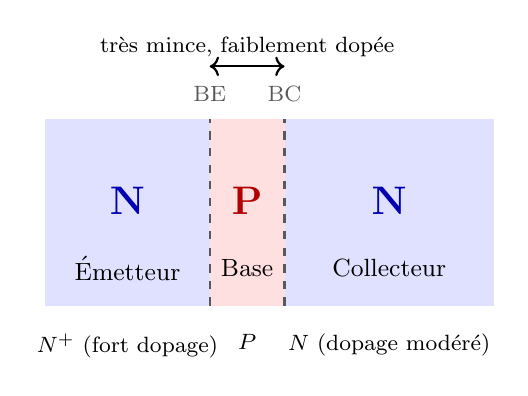
\begin{tikzpicture}[scale=0.95]
  \fill[blue!12] (0,0) rectangle (2.2,2.5);
  \fill[red!12] (2.2,0) rectangle (3.2,2.5);
  \fill[blue!12] (3.2,0) rectangle (6,2.5);
  \node[font=\Large\bfseries, blue!70!black] at (1.1,1.4) {N};
  \node[font=\Large\bfseries, red!70!black] at (2.7,1.4) {P};
  \node[font=\Large\bfseries, blue!70!black] at (4.6,1.4) {N};
  \node[font=\small] at (1.1,0.5) {Émetteur};
  \node[font=\small] at (2.7,0.5) {Base};
  \node[font=\small] at (4.6,0.5) {Collecteur};
  \draw[dashed, thick, gray!70!black] (2.2,0) -- (2.2,2.5);
  \draw[dashed, thick, gray!70!black] (3.2,0) -- (3.2,2.5);
  \node[font=\footnotesize, gray!70!black, above] at (2.2,2.6) {BE};
  \node[font=\footnotesize, gray!70!black, above] at (3.2,2.6) {BC};
  \draw[<->, thick] (2.2,3.2) -- (3.2,3.2);
  \node[font=\footnotesize, above] at (2.7,3.2) {très mince, faiblement dopée};
  \node[font=\footnotesize, below] at (1.1,-0.25) {$N^+$ (fort dopage)};
  \node[font=\footnotesize, below] at (2.7,-0.25) {$P$};
  \node[font=\footnotesize, below] at (4.6,-0.25) {$N$ (dopage modéré)};
\end{tikzpicture}
\end{center}

\subsubsection*{La chaîne causale physique}

La séquence physique qui crée le courant collecteur est :

\begin{formule}
\[
\boxed{V_{BE} \xrightarrow{\text{1. abaisse la barrière}} \text{injection d'électrons} \xrightarrow{\text{2. diffusion}} \text{traversée de la base} \xrightarrow{\text{3. collecte}} I_C}
\]
\begin{enumerate}[nosep]
\item $V_{BE}$ en polarisation directe \textbf{abaisse la barrière de potentiel} de la jonction BE. Les électrons de l'émetteur ($N^+$, fortement dopé) sont injectés massivement dans la base P.
\item Les électrons injectés \textbf{diffusent} à travers la base mince. Comme la base est très mince ($W_B \ll L_n$, longueur de diffusion) et faiblement dopée, la \textit{grande majorité} des électrons traverse sans se recombiner.
\item Les électrons qui arrivent à la jonction BC (polarisée en inverse en régime actif) sont \textbf{aspirés} par le champ électrique de la zone de déplétion vers le collecteur $\Rightarrow$ courant $I_C$.
\end{enumerate}

\textbf{Et le courant de base $I_B$ ?} C'est la \textit{conséquence} de deux phénomènes mineurs :
\begin{itemize}[nosep]
\item Les quelques recombinaisons dans la base (électrons qui ``disparaissent'' en se recombinant avec des trous) $\Rightarrow$ il faut fournir des trous de remplacement.
\item L'injection de trous de la base P vers l'émetteur $N^+$ (courant inverse de la jonction BE, faible car l'émetteur est beaucoup plus dopé).
\end{itemize}
\end{formule}

\begin{attention}
\textbf{$I_B$ n'est pas la cause de $I_C$.} C'est $V_{BE}$ qui contrôle l'injection. $I_B$ est un ``effet secondaire'' des recombinaisons. Le gain $\beta = I_C/I_B$ est élevé \textit{parce que} la base est mince et faiblement dopée (peu de recombinaisons), pas parce que le transistor ``amplifie le courant de base''.

Cette distinction est fondamentale pour comprendre :
\begin{itemize}[nosep]
\item pourquoi $\beta$ varie (il dépend des recombinaisons, pas d'un mécanisme fondamental),
\item pourquoi le modèle petit signal utilise $g_m = \partial I_C/\partial V_{BE}$ (commandé en tension),
\item pourquoi la conception de circuits intégrés ne repose jamais sur $\beta$.
\end{itemize}
\end{attention}

\subsection{L'équation de Shockley pour le BJT}

\begin{formule}
\[
\boxed{I_C = I_S\,e^{V_{BE}/V_T}\left(1 + \frac{V_{CE}}{V_A}\right)}
\]
\textbf{Hypothèses :} régime actif direct, modèle d'Ebers-Moll simplifié.

\begin{itemize}[nosep]
\item $I_S$ : courant de saturation inverse ($\sim\SI{1e-15}{A}$ à $\SI{1e-12}{A}$). Dépend \textbf{fortement} de la température : $I_S \propto T^4 e^{-E_g/kT}$, approximativement $\times 2$ tous les \SI{10}{°C}.
\item $V_T = kT/q$ : tension thermique (\SI{25.85}{mV} à \SI{25}{°C}, \SI{33.5}{mV} à \SI{125}{°C}).
\item $V_A$ : tension d'Early (\SI{50}{V} à \SI{200}{V}), modélise la dépendance de $I_C$ en $V_{CE}$.
\item Le terme $(1 + V_{CE}/V_A)$ est souvent omis en première approximation.
\end{itemize}
\end{formule}

\begin{intuition}
\textbf{Sensibilité exponentielle :} une variation de $V_{BE}$ de seulement $\SI{60}{mV}$ (à $n = 1$, \SI{25}{°C}) multiplie $I_C$ par \textbf{10}. C'est cette sensibilité extraordinaire qui rend le BJT excellent pour l'amplification de précision, mais aussi très sensible aux variations de température ($V_{BE}$ diminue d'environ $\SI{-2}{mV/°C}$ à courant constant).
\end{intuition}

\subsection{Polarisation par diviseur de tension}

Pour utiliser un BJT en amplification, il faut fixer un \textbf{point de repos} $Q = (I_{C,Q}, V_{CE,Q})$ stable en régime actif.

\begin{center}
\begin{circuitikz}[scale=0.9, american]
  \draw (4,6) node[above]{$V_{CC}$} -- (4,5.5);
  \draw (4,5.5) to[R, l=$R_C$, i>=$I_C$] (4,3.5);
  \draw (4,3.5) -- (4,3.2);
  \draw (2.5,2.5) node[npn, anchor=B](Q){};
  \draw (Q.C) -- (4,3.2);
  \draw (Q.E) -- (2.5,1.2);
  \draw (2.5,1.2) to[R, l=$R_E$] (2.5,-0.5) node[ground]{};
  \draw (0,6) node[above]{$V_{CC}$} -- (0,5.5);
  \draw (0,5.5) to[R, l=$R_1$] (0,2.5);
  \draw (0,2.5) to[R, l=$R_2$] (0,-0.5) node[ground]{};
  \draw (0,2.5) -- (Q.B);
  \filldraw (0,2.5) circle (1.5pt);
  \node[above, font=\footnotesize] at (1.3,2.55) {$V_B$};
  \node[font=\footnotesize] at (3.5,1.5) {$V_E$};
\end{circuitikz}
\end{center}

\begin{formule}
\textbf{Calcul du point de repos} (hypothèse : $I_B \ll I_{\text{div}} = V_{CC}/(R_1+R_2)$) :
\[
V_B = V_{CC}\frac{R_2}{R_1+R_2}, \qquad V_E = V_B - V_{BE,Q}, \qquad I_C \approx I_E = \frac{V_E}{R_E}, \qquad V_{CE} = V_{CC} - I_C(R_C+R_E)
\]
\textbf{Vérifications :} $V_{CE} > V_{CE,\text{sat}}$ (régime actif), et $I_B/I_{\text{div}} < 10\%$ (validité du diviseur).
\end{formule}

\begin{intuition}
\textbf{Le rôle stabilisateur de $R_E$ :} si $T$ augmente $\Rightarrow$ $I_S$ augmente $\Rightarrow$ $I_C$ tend à augmenter. Mais $I_C \uparrow$ $\Rightarrow$ $V_E = R_E I_E \uparrow$ $\Rightarrow$ $V_{BE} = V_B - V_E \downarrow$ $\Rightarrow$ $I_C \downarrow$ (par l'exponentielle). C'est une \textbf{rétroaction négative} intrinsèque. Sans $R_E$, le point de repos dérive avec la température et peut conduire à l'emballement thermique.
\end{intuition}

\subsection{Dérivation du modèle petit signal hybride-$\pi$}

\subsubsection*{Principe : linéarisation autour de $Q$}

Le transistor est non-linéaire ($I_C \propto e^{V_{BE}/V_T}$). Pour analyser les signaux AC, on \textbf{linéarise} autour du point de repos $Q$ en séparant composante DC et petite variation AC :

\begin{formule}
\[
V_{BE}(t) = \underbrace{V_{BE,Q}}_{\text{DC}} + \underbrace{v_{be}(t)}_{\text{AC}} \qquad \text{avec } |v_{be}| \ll V_T \approx \SI{26}{mV}
\]
Convention : \textbf{majuscules = DC}, \textbf{minuscules = AC (petit signal)}.
\end{formule}

\subsubsection*{La transconductance $g_m$}

On développe $I_C = I_S e^{V_{BE}/V_T}$ au premier ordre (Taylor, $e^x \approx 1+x$ pour $|x| \ll 1$) :
\[
I_C \approx I_{C,Q}\left(1 + \frac{v_{be}}{V_T}\right) = I_{C,Q} + \underbrace{\frac{I_{C,Q}}{V_T}}_{g_m}\,v_{be}
\]

\begin{formule}
\[
\boxed{g_m = \frac{\partial I_C}{\partial V_{BE}}\bigg|_Q = \frac{I_{C,Q}}{V_T}}
\]
\textbf{Validité :} petit signal ($|v_{be}| \ll V_T$). En pratique, $|v_{be}| < \SI{5}{mV}$ pour une distorsion $< 1\%$ (THD), $< \SI{10}{mV}$ pour $< 5\%$. Au-delà, les termes d'ordre supérieur ne sont plus négligeables.

\textbf{Remarque fondamentale :} $g_m$ ne dépend \textit{que} du courant de polarisation $I_{C,Q}$ et de la température (via $V_T$). Il est \textbf{indépendant de $\beta$}, de la géométrie du transistor, et de la technologie. C'est une propriété universelle de la jonction PN.
\end{formule}

\subsubsection*{La résistance d'entrée $r_\pi$}

Le courant de base AC est $i_b = i_c/\beta = g_m v_{be}/\beta$. On en déduit :

\begin{formule}
\[
\boxed{r_\pi = \frac{v_{be}}{i_b} = \frac{\beta}{g_m} = \frac{\beta V_T}{I_{C,Q}}}
\]
$r_\pi$ est la résistance d'entrée vue entre base et émetteur en petit signal. Contrairement à $g_m$, elle dépend de $\beta$ et varie donc d'un transistor à l'autre.
\end{formule}

\subsubsection*{La résistance de sortie $r_o$ (effet Early)}

Le courant $I_C$ dépend légèrement de $V_{CE}$ via le terme $(1 + V_{CE}/V_A)$. En petit signal :

\begin{formule}
\[
\boxed{r_o = \frac{\partial V_{CE}}{\partial I_C}\bigg|_Q \approx \frac{V_A}{I_{C,Q}}}
\]
$r_o$ représente le fait que le collecteur n'est pas une source de courant parfaite. Le gain intrinsèque maximal d'un étage est $A_{v,\max} = g_m r_o = V_A/V_T \approx 2000$--$8000$ selon le transistor.
\end{formule}

\subsubsection*{Le schéma équivalent}

\begin{center}
\begin{circuitikz}[scale=1.0, american]
  \node[left, font=\small] at (0,0) {B};
  \node[right, font=\small] at (8,0) {C};
  \node[left, font=\small] at (0,-3) {E};
  \node[right, font=\small] at (8,-3) {E};
  \draw (0,0) -- (2,0);
  \draw (2,0) to[R, l=$r_\pi$] (2,-3);
  \draw (0,-3) -- (8,-3);
  \draw (4.5,0) to[american controlled current source, l_=$g_m\,v_{be}$] (4.5,-3);
  \draw (2,0) -- (4.5,0);
  \draw (7,0) to[R, l=$r_o$] (7,-3);
  \draw (4.5,0) -- (7,0);
  \draw (7,0) -- (8,0);
  \filldraw (2,0) circle (1.5pt);
  \filldraw (2,-3) circle (1.5pt);
  \filldraw (4.5,0) circle (1.5pt);
  \filldraw (4.5,-3) circle (1.5pt);
  \filldraw (7,0) circle (1.5pt);
  \filldraw (7,-3) circle (1.5pt);
  \draw[{Stealth[length=2.5mm]}-{Stealth[length=2.5mm]}, thick] (1,-0.15) -- (1,-2.85);
  \node[font=\small, left] at (0.95,-1.5) {$v_{be}$};
\end{circuitikz}
\end{center}

\begin{intuition}
\textbf{Comment lire le modèle :}
\begin{itemize}[nosep]
\item \textbf{Côté entrée (B-E)} : $r_\pi$ est l'impédance d'entrée. Un signal $v_{be}$ crée $i_b = v_{be}/r_\pi$.
\item \textbf{Côté sortie (C-E)} : la source commandée $g_m v_{be}$ convertit la tension d'entrée en courant de sortie. C'est le mécanisme d'amplification.
\item $r_o$ en parallèle : la source de courant n'est pas idéale (effet Early).
\item \textbf{Ce modèle est valide en basse fréquence.} En HF, il faut ajouter les capacités parasites $C_\pi$ (BE) et $C_\mu$ (BC) — voir niveau ingénieur.
\end{itemize}
\end{intuition}

\subsection{Gain en tension de l'émetteur commun}

\begin{formule}
\textbf{Avec $R_E$ découplée} (condensateur de bypass) :
\[
\boxed{A_v = -g_m(R_C \parallel r_o) \approx -g_m R_C = -\frac{I_{C,Q} R_C}{V_T}}
\]
Le gain est inverseur et indépendant de $\beta$.

\textbf{Sans découplage} (condition : $g_m R_E \gg 1$, presque toujours vérifié) :
\[
\boxed{A_v \approx -\frac{R_C}{R_E}}
\]
Le gain ne dépend que de résistances : indépendant de $g_m$, $I_C$, $T$ et $\beta$. C'est le compromis gain/stabilité/linéarité utilisé en audio de précision.
\end{formule}

\subsection{Le collecteur commun (émetteur suiveur) : le buffer}

L'émetteur commun amplifie la tension. Mais que faire quand le problème n'est pas le gain, mais l'\textbf{impédance} --- une source fragile (capteur, filtre du chapitre 14) qui doit piloter une charge gourmande ? Réponse : le \textbf{collecteur commun}, dit \textbf{émetteur suiveur}.

\begin{center}
\begin{circuitikz}[scale=0.95, american]
  % Transistor
  \draw (3,2) node[npn, anchor=B](Q){};
  % Collecteur direct à VCC
  \draw (Q.C) -- ++(0,1.2) node[above]{$V_{CC}$};
  % Base : entrée
  \draw (Q.B) -- ++(-1.6,0) node[left]{$v_{\text{in}}$};
  % Émetteur : RE vers masse + sortie
  \draw (Q.E) to[R, l_=$R_E$, i=$i_E$] ++(0,-2.4) node[ground]{};
  \draw (Q.E) -- ++(1.8,0) node[right]{$v_{\text{out}}$};
  \filldraw (Q.E) circle (1.5pt);
\end{circuitikz}
\end{center}

\begin{formule}
\textbf{Hypothèses :} régime actif, petit signal, $r_o \gg R_E$.

\textbf{Gain en tension} (la sortie ``suit'' l'entrée à $V_{BE}$ près) :
\[
\boxed{A_v = \frac{g_m R_E}{1 + g_m R_E} \approx 1 \quad (\text{non inverseur, légèrement} < 1)}
\]

\textbf{Impédance d'entrée} --- la charge est vue \textit{multipliée par} $(\beta+1)$ :
\[
\boxed{Z_{\text{in}} = r_\pi + (\beta+1)R_E} \qquad \text{(élevée : centaines de k}\Omega\text{)}
\]

\textbf{Impédance de sortie} --- la résistance de source est vue \textit{divisée par} $(\beta+1)$ :
\[
\boxed{Z_{\text{out}} \approx \frac{1}{g_m} + \frac{R_s}{\beta+1}} \qquad \text{(faible : quelques dizaines d'}\Omega\text{)}
\]
\end{formule}

\begin{intuition}
\textbf{Le suiveur est un transformateur d'impédance, pas un amplificateur de tension.} Il ne gagne ``rien'' ($A_v \approx 1$) mais son gain en \textit{courant} vaut $\approx \beta+1$ : il y a bien gain en \textbf{puissance}. C'est exactement le rôle du suiveur AOP (chapitre 18) en version transistor --- et c'est l'étage de sortie de la plupart des montages : il isole l'amplification (faite en amont par un EC) de la charge.
\end{intuition}

\subsection{La base commune : l'étage haute fréquence}

\begin{formule}
\textbf{Base à la masse (en alternatif), signal injecté dans l'émetteur, sortie sur le collecteur.}

\textbf{Hypothèses :} régime actif, petit signal.
\[
A_v = +g_m R_C \;\; (\text{non inverseur}) \qquad Z_{\text{in}} \approx \frac{1}{g_m} \;\; (\text{très faible : quelques dizaines d'}\Omega) \qquad Z_{\text{out}} \approx R_C
\]

\textbf{La propriété décisive : pas d'effet Miller.} La base étant à la masse, $C_\mu$ n'est pas ``multipliée'' par le gain (voir section suivante) : la bande passante est \textbf{maximale}. C'est précisément pour cela que le cascode (niveau ingénieur) confie l'étage de sortie à une base commune.

\textbf{Usages :} étages HF/RF, cascode, et réception de signaux en \textit{courant} (photodiode, ligne $\SI{50}{\ohm}$) où la faible $Z_{\text{in}}$ est un atout.
\end{formule}

\subsection{Tableau comparatif : choisir son montage}

\begin{pratique}
\begin{center}
\renewcommand{\arraystretch}{1.45}
\begin{tabular}{p{2.9cm}p{3.1cm}p{3.1cm}p{3.3cm}}
\toprule
\textbf{Critère} & \textbf{Émetteur commun} & \textbf{Collecteur commun} & \textbf{Base commune} \\
\midrule
Gain en tension & $-g_m R_C$ (élevé, inverseur) & $\approx 1$ (non inverseur) & $+g_m R_C$ (élevé, non inverseur) \\
Gain en courant & $\beta$ & $\beta + 1$ & $\approx 1$ ($\alpha$) \\
$Z_{\text{in}}$ & $r_\pi$ (moyenne, k$\Omega$) & $r_\pi + (\beta{+}1)R_E$ (\textbf{élevée}) & $1/g_m$ (\textbf{très faible}) \\
$Z_{\text{out}}$ & $R_C$ (moyenne) & $1/g_m + R_s/(\beta{+}1)$ (\textbf{faible}) & $R_C$ (moyenne) \\
Bande passante & Limitée (Miller) & Large & \textbf{Maximale} (pas de Miller) \\
Rôle type & \textbf{Amplifier} la tension & \textbf{Isoler} (buffer) & \textbf{Monter en fréquence} \\
\bottomrule
\end{tabular}
\end{center}

\textbf{Réflexe de conception :} un amplificateur complet enchaîne souvent les trois --- EC pour le gain, BC pour la bande passante (cascode), CC pour piloter la charge. Les trois montages sont les trois outils d'une même boîte, pas trois concurrents.
\end{pratique}

% ============================================================================
\section{Niveau Ingénieur}

\begin{ingenieur}
Modèle physique complet : réponse en fréquence ($C_\pi$, $C_\mu$, $f_T$), effet Miller, emballement thermique, bruit, saturation profonde, et technologies modernes (SiGe HBT, BiCMOS).
\end{ingenieur}

\subsection{Réponse en fréquence : $C_\pi$, $C_\mu$ et $f_T$}

En haute fréquence, deux capacités parasites s'ajoutent au modèle hybride-$\pi$ :

\begin{formule}
\begin{itemize}[nosep]
\item $C_\pi = C_{\text{diff}} + C_{\text{dep,BE}}$ : capacité base-émetteur. La composante de diffusion $C_{\text{diff}} = g_m \tau_F$ (proportionnelle à $I_C$) domine en régime actif. $\tau_F$ est le temps de transit dans la base ($\sim\SI{10}{ps}$ à \SI{1}{ns}).
\item $C_\mu = C_{\text{dep,BC}}$ : capacité base-collecteur (jonction BC en inverse, quelques pF, peu variable avec $I_C$).
\end{itemize}

La \textbf{fréquence de transition} $f_T$ est la fréquence où le gain en courant $|\beta(f)| = 1$ :
\[
\boxed{f_T = \frac{g_m}{2\pi(C_\pi + C_\mu)}}
\]
Typiquement : \SI{300}{MHz} (2N2222), \SI{5}{GHz} (BFR92), \SI{200}{GHz}+ (SiGe HBT).
\end{formule}

\subsection{L'effet Miller et le cascode}

\begin{formule}
Dans le montage émetteur commun, $C_\mu$ est ``multipliée'' par le gain et apparaît comme une capacité effective à l'entrée :
\[
\boxed{C_{\text{Miller}} = C_\mu(1 + |A_v|)}
\]
\textbf{Exemple :} $C_\mu = \SI{4}{pF}$, $A_v = -180$ $\Rightarrow$ $C_{\text{Miller}} = \SI{724}{pF}$. Avec une source de $R_s = \SI{1}{k\ohm}$ : $f_{-3\text{dB}} = 1/(2\pi R_s C_{\text{in}}) \approx \SI{250}{kHz}$ seulement.
\end{formule}

\begin{pratique}
\textbf{Le montage cascode} (émetteur commun + base commune) supprime l'effet Miller car le gain local de l'étage EC est $\approx 1$ (collecteur de l'EC vu à basse impédance par l'émetteur de la BC). $C_{\text{Miller}} \approx 2C_\mu$ au lieu de $C_\mu(1+|A_v|)$ $\Rightarrow$ gain en bande passante typique de $\times 10$ à $\times 100$.
\end{pratique}

\subsection{Le miroir de courant : la brique des circuits intégrés}

\begin{center}
\begin{circuitikz}[scale=0.95, american]
  % Q1 diode-connecté (gauche, miroir horizontal)
  \draw (0,1.2) node[npn, xscale=-1, anchor=B](Q1){};
  % Q2 (droite)
  \draw (3.4,1.2) node[npn, anchor=B](Q2){};
  % Bases communes
  \draw (Q1.B) -- (Q2.B);
  \filldraw (1.7,1.2) circle (1.5pt);
  % Diode-connexion : C de Q1 relié à la ligne des bases
  \draw (Q1.C) -| (1.7,1.2);
  \filldraw (Q1.C) circle (1.5pt);
  % Courants d'entrée et de sortie
  \draw (Q1.C) ++(0,1.4) node[above]{$I_{\text{ref}}$ (depuis $R_{\text{ref}}$)} to[short, i=$ $] (Q1.C);
  \draw (Q2.C) ++(0,1.4) node[above]{$I_{\text{out}}$ (vers la charge)} to[short, i=$ $] (Q2.C);
  % Émetteurs à la masse
  \draw (Q1.E) -- ++(0,-0.5) node[ground]{};
  \draw (Q2.E) -- ++(0,-0.5) node[ground]{};
\end{circuitikz}
\end{center}

\begin{formule}
\textbf{Principe :} $Q_1$ est ``monté en diode'' (collecteur relié à la base) : le courant $I_{\text{ref}}$ qui le traverse impose son $V_{BE}$. Ce $V_{BE}$ est appliqué tel quel à $Q_2$. Si les deux transistors sont \textbf{appariés} (même puce, même température, même géométrie), l'équation de Shockley donne :
\[
\boxed{I_{\text{out}} \approx I_{\text{ref}}}
\]
Le courant est ``recopié'' --- d'où le nom de miroir.

\textbf{Hypothèses et erreurs réelles :}
\begin{itemize}[nosep]
\item \textbf{Courants de base} : $I_{\text{ref}}$ alimente aussi les deux bases $\Rightarrow$ erreur relative $\approx -2/\beta$ ($-1\%$ pour $\beta = 200$).
\item \textbf{Effet Early} : si $V_{CE2} \neq V_{CE1} = V_{BE}$, alors $I_{\text{out}} = I_{\text{ref}}(1 + (V_{CE2}-V_{BE})/V_A)$. Pour $V_A = \SI{100}{V}$ et $\Delta V_{CE} = \SI{5}{V}$ : $+5\%$ d'erreur. C'est l'erreur dominante.
\item \textbf{Remèdes} : miroir \textbf{cascode} (rigidifie $V_{CE1} = V_{CE2}$) ou miroir de \textbf{Wilson} (rétroaction qui compense les courants de base). Précision typique : $0{,}1\%$.
\end{itemize}
\end{formule}

\begin{intuition}
\textbf{Pourquoi le miroir est partout en circuit intégré :} sur une puce, les résistances précises sont chères en surface et dérivent ; les transistors appariés sont gratuits et suivent ensemble la température. Le miroir sert donc (1) à \textbf{distribuer les polarisations} (une seule référence, recopiée partout), et (2) comme \textbf{charge active} : remplacer $R_C$ par la sortie d'un miroir PNP donne un gain $A_v = -g_m(r_{o,n} \parallel r_{o,p})$ au lieu de $-g_m R_C$ --- des gains de $1000$ à $10\,000$ par étage, impossibles avec une résistance (qui exigerait des dizaines de volts d'alimentation). C'est exactement ainsi que l'AOP du chapitre 18 obtient son gain colossal.
\end{intuition}

\subsection{La paire différentielle : amplifier une différence}

\begin{formule}
\textbf{Structure :} deux transistors identiques dont les émetteurs sont reliés à une \textbf{source de courant} commune $I_{\text{tail}}$ (réalisée\ldots par un miroir). Les entrées sont les deux bases ; les sorties, les deux collecteurs.

\textbf{Principe :} $I_{\text{tail}}$ se répartit entre $Q_1$ et $Q_2$ selon la différence d'entrée $v_d = v_1 - v_2$ :
\[
I_{C1} = \frac{I_{\text{tail}}}{1 + e^{-v_d/V_T}} \qquad I_{C2} = \frac{I_{\text{tail}}}{1 + e^{+v_d/V_T}}
\]
\begin{itemize}[nosep]
\item $v_d = 0$ : équilibre parfait, $I_{C1} = I_{C2} = I_{\text{tail}}/2$.
\item $|v_d| \gtrsim 4V_T \approx \SI{100}{mV}$ : \textbf{tout} le courant bascule d'un côté --- c'est ce basculement complet qui fixe le slew rate de l'AOP (chapitre 18 : $SR = I_{\text{tail}}/C_C$).
\end{itemize}

\textbf{En petit signal} ($|v_d| \ll V_T$), chaque transistor est polarisé à $I_{\text{tail}}/2$ :
\[
\boxed{A_{v,\text{diff}} = -g_m R_C \quad \text{avec} \quad g_m = \frac{I_{\text{tail}}/2}{V_T}}
\]

\textbf{Réjection du mode commun :} si $v_1$ et $v_2$ montent \textit{ensemble} (parasite, dérive), la source de courant maintient $I_{\text{tail}}$ constant $\Rightarrow$ rien ne change en sortie. Le \textbf{CMRR} (rapport de réjection) est directement fixé par la qualité (le $r_o$) de la source de courant de queue : encore le miroir.
\end{formule}

\begin{intuition}
\textbf{La paire différentielle est la cellule d'entrée universelle} : c'est l'étage 1 de tous les AOP (chapitre 18), des comparateurs, et même du sense amplifier des mémoires (chapitre 24). Sa force : elle ne mesure que la \textit{différence}, en ignorant tout ce qui est commun aux deux entrées --- bruit d'alimentation, température, dérives. Associée à une charge active en miroir, elle fournit l'essentiel du gain d'un AOP.
\end{intuition}

\subsection{Les étages de sortie : classes A, B et AB}

\begin{formule}
Délivrer de la \textit{puissance} à une charge (haut-parleur, ligne, moteur) pose un problème que le petit signal ignore : le \textbf{rendement}.

\textbf{Classe A} : un transistor unique conduit en permanence (360°), polarisé au milieu de sa droite de charge. Linéaire, simple --- mais le courant de repos dissipe en permanence :
\[
\eta_{\max} = 25\% \;\;(\text{charge résistive directe})
\]
Un ampli classe A de $\SI{10}{W}$ utiles dissipe $\geq \SI{30}{W}$ \textit{au repos}.

\textbf{Classe B} : deux transistors complémentaires (NPN + PNP) en \textbf{push-pull}, chacun conduisant une demi-alternance (180°). Au repos, courant nul :
\[
\eta_{\max} = \frac{\pi}{4} \approx 78{,}5\%
\]
\textbf{Mais} : autour de zéro, \textit{aucun} des deux ne conduit tant que $|v_{\text{in}}| < V_{BE} \approx \SI{0.6}{V}$ $\Rightarrow$ \textbf{distorsion de croisement} (\textit{crossover}), une zone morte de $\sim\SI{1.2}{V}$ très audible et très visible au spectre.

\textbf{Classe AB} : on pré-polarise les deux bases avec $\approx 2V_{BE}$ (deux diodes ou un \textbf{multiplicateur de $V_{BE}$}) pour qu'un \textit{léger} courant de repos circule. La zone morte disparaît, le rendement reste proche de la classe B ($60$--$70\%$ en pratique). \textbf{C'est l'étage de sortie standard} --- y compris celui de l'AOP du chapitre 18.
\end{formule}

\begin{attention}
\textbf{Stabilité thermique de la classe AB :} le courant de repos dépend de l'écart entre la tension des diodes de polarisation et les $V_{BE}$ des transistors de puissance. Si les transistors chauffent ($V_{BE}$ diminue de $\SI{-2}{mV/°C}$) mais pas les diodes, le courant de repos \textbf{augmente}, donc la dissipation augmente, donc la température monte\ldots C'est exactement le mécanisme d'emballement thermique de la section suivante. \textbf{Parade obligatoire :} monter les diodes de polarisation \textit{sur le même radiateur} que les transistors de puissance (couplage thermique), et ajouter de petites résistances d'émetteur ($0{,}1$--$\SI{0.5}{\ohm}$) en dégénérescence.
\end{attention}

\subsection{L'emballement thermique}

\begin{attention}
\textbf{Boucle de rétroaction positive :}
\[
T \uparrow \;\Rightarrow\; I_S \uparrow \;\Rightarrow\; I_C \uparrow \text{ (à $V_{BE}$ constant)} \;\Rightarrow\; P = V_{CE}I_C \uparrow \;\Rightarrow\; T \uparrow
\]
$I_S$ double environ tous les \SI{10}{°C}. À $V_{BE}$ constant, le courant collecteur augmente de $\approx 8{,}7\%/°$C.

\textbf{Condition de stabilité thermique} (critère simplifié) :
\[
\frac{\partial P}{\partial T}\bigg|_Q < \frac{1}{R_{\theta JA}}
\]
où $R_{\theta JA}$ est la résistance thermique jonction-ambiant (°C/W).

\textbf{Protections :}
\begin{itemize}[nosep]
\item $R_E$ non nulle : rétroaction négative sur $V_{BE}$ (vu en polarisation).
\item Résistances d'émetteur individuelles pour les transistors en parallèle.
\item Dimensionnement thermique : radiateur adapté.
\end{itemize}

\textbf{Comparaison MOSFET :} le MOSFET est naturellement stable car $R_{DS,\text{on}}$ \textit{augmente} avec la température (coefficient positif de la mobilité $\mu$). Pas d'emballement possible.
\end{attention}

\subsection{Saturation profonde et temps de stockage}

En saturation, les \textit{deux} jonctions (BE et BC) sont polarisées en direct. Des porteurs minoritaires excédentaires sont injectés et \textbf{stockés dans la base}. Cette charge stockée $Q_s$ doit être évacuée avant que le transistor puisse se bloquer :

\begin{formule}
\[
t_s \approx \tau_s \ln\left(\frac{I_{B,\text{on}} - I_{C}/\beta}{I_{B,\text{off}} + I_C/\beta}\right)
\]
avec $\tau_s$ le temps de vie des porteurs dans la base en saturation.

\textbf{Conséquence :} le BJT a un temps de commutation ON $\to$ OFF plus long que le MOSFET (qui n'a pas de charges stockées dans le canal).
\end{formule}

\subsection{Bruit dans le BJT}

Le BJT est un composant \textbf{remarquablement peu bruyant}, ce qui explique sa prédominance en amplification RF basse bruit et en audio de précision.

\begin{formule}
\textbf{Sources de bruit principales :}
\begin{itemize}[nosep]
\item \textbf{Bruit de grenaille (shot noise)} sur $I_C$ et $I_B$ : $\overline{i_c^2} = 2qI_C\Delta f$ et $\overline{i_b^2} = 2qI_B\Delta f$. C'est la nature quantique du passage des porteurs à travers une barrière de potentiel.
\item \textbf{Bruit thermique} de la résistance de base $r_b$ : $\overline{v_b^2} = 4kTr_b\Delta f$.
\item \textbf{Bruit $1/f$ (flicker)} : faible dans le BJT car les porteurs traversent le \textit{volume} du cristal (pas la surface). C'est un avantage majeur par rapport au MOSFET dont le canal est à l'interface Si/SiO$_2$ (riche en pièges).
\end{itemize}

Le \textbf{facteur de bruit} $NF$ minimal est atteint pour un courant optimal $I_{C,\text{opt}} \approx V_T/(R_s \sqrt{\beta})$.
\end{formule}

\subsection{Technologies modernes}

\begin{pratique}
Le BJT silicium classique a été largement remplacé par le MOSFET en logique et en puissance. Mais il reste incontournable sous des formes évoluées :

\begin{itemize}[nosep]
\item \textbf{SiGe HBT} (\textit{Heterojunction Bipolar Transistor}) : un alliage SiGe dans la base crée un champ de dérive qui accélère les porteurs. $f_T > \SI{300}{GHz}$, bruit $NF < \SI{0.5}{dB}$. Utilisé dans les LNA 5G, les PLL millimétriques, et les ADC ultra-rapides.
\item \textbf{BiCMOS} : technologie qui combine BJT (pour l'analogique de précision, les références de tension, les LNA) et CMOS (pour la logique numérique) sur la même puce.
\item \textbf{Bandgap} : la dépendance complémentaire de $V_{BE}$ en température ($\SI{-2}{mV/°C}$) est exploitée avec une tension proportionnelle à $T$ ($V_T$) pour créer des références de tension ultra-stables ($\sim\SI{1.2}{V}$, $< \SI{10}{ppm/°C}$).
\end{itemize}
\end{pratique}

% === EXERCICES ===
\section*{Exercices}
\addcontentsline{toc}{section}{Exercices}

\subsection*{Niveau débutant}

\textbf{Exercice 16.1 ---} Un transistor NPN a $\beta = 150$. On impose $I_B = \SI{50}{\micro A}$. Calculez $I_C$ et $I_E$. Pourquoi est-il incorrect de dire que ``$I_B$ \textit{cause} $I_C$'' ?

\begin{pratique}
\textbf{Solution :} $I_C = \beta I_B = 150\times50\times10^{-6} = \SI{7.5}{mA}$. $I_E = I_B + I_C = \SI{7.55}{mA}$.

Physiquement, c'est la \textit{tension} $V_{BE}$ qui contrôle l'injection de porteurs et donc $I_C$. Quand on ``impose $I_B$'', on fixe en réalité $V_{BE}$ (via la caractéristique exponentielle de la jonction BE), et c'est ce $V_{BE}$ qui détermine $I_C$. $I_B$ est une conséquence des recombinaisons dans la base, pas la cause de $I_C$.
\end{pratique}

\textbf{Exercice 16.2 ---} Dimensionnez $R_B$ pour piloter un relais ($R_{\text{bobine}} = \SI{200}{\ohm}$) sous $V_{CC} = \SI{12}{V}$ depuis un GPIO \SI{3.3}{V} avec un 2N2222 ($\beta_{\min} = 75$). Facteur de sursaturation $k = 3$.

\begin{pratique}
\textbf{Solution :} $I_C = (12-0{,}2)/200 = \SI{59}{mA}$. $I_{B,\min} = 59/75 = \SI{0.79}{mA}$. $I_B = 3\times0{,}79 = \SI{2.4}{mA}$. $R_B = (3{,}3 - 0{,}7)/2{,}4\times10^{-3} = \SI{1083}{\ohm} \to \SI{1}{k\ohm}$ (E24). Diode de roue libre obligatoire.
\end{pratique}

\subsection*{Niveau intermédiaire}

\textbf{Exercice 16.3 ---} Amplificateur EC : $V_{CC} = \SI{12}{V}$, $R_1 = \SI{56}{k\ohm}$, $R_2 = \SI{12}{k\ohm}$, $R_C = \SI{3.3}{k\ohm}$, $R_E = \SI{1}{k\ohm}$, $\beta = 200$. Calculez le point de repos, $g_m$, $r_\pi$, et le gain avec et sans découplage de $R_E$.

\begin{pratique}
\textbf{Solution :} $V_B = 12\times12/68 = \SI{2.12}{V}$. $V_E = 2{,}12 - 0{,}7 = \SI{1.42}{V}$. $I_C \approx 1{,}42/1000 = \SI{1.42}{mA}$. $V_{CE} = 12 - 1{,}42\times4{,}3 = \SI{5.89}{V}$ (actif confirmé). $I_B/I_{\text{div}} = 7{,}1\mu/176\mu = 4\%$ (hypothèse validée).

$g_m = 1{,}42\times10^{-3}/0{,}026 = \SI{54.6}{mA/V}$. $r_\pi = 200/54{,}6\times10^{-3} = \SI{3.66}{k\ohm}$.

Avec découplage : $A_v = -g_m R_C = -180$ (\SI{45}{dB}).

Sans découplage : $A_v \approx -R_C/R_E = -3{,}3$ (\SI{10}{dB}). Gain beaucoup plus faible mais totalement indépendant de $g_m$, $\beta$ et $T$.
\end{pratique}

\subsection*{Niveau ingénieur}

\textbf{Exercice 16.4 ---} BC547 ($f_T = \SI{300}{MHz}$, $C_\mu = \SI{3.5}{pF}$, $\beta = 300$, $V_A = \SI{100}{V}$) en EC, $I_C = \SI{2}{mA}$, $R_C = \SI{2.2}{k\ohm}$, $R_s = \SI{1}{k\ohm}$. Calculez l'effet Miller et la bande passante, puis comparez avec un cascode.

\begin{pratique}
\textbf{Solution :} $g_m = \SI{76.9}{mA/V}$. $A_v = -169$. $C_{\text{Miller}} = 3{,}5\times170 = \SI{595}{pF}$.

$C_\pi = g_m/(2\pi f_T) - C_\mu = 40{,}8 - 3{,}5 = \SI{37.3}{pF}$. $C_{\text{in}} = 37{,}3 + 595 = \SI{632}{pF}$.

$f_{-3\text{dB}} = 1/(2\pi\times10^3\times632\times10^{-12}) = \SI{252}{kHz}$.

Cascode : $C_{\text{Miller}} \approx 2\times3{,}5 = \SI{7}{pF}$. $C_{\text{in}} = 37{,}3+7 = \SI{44.3}{pF}$. $f_{-3\text{dB}} = \SI{3.6}{MHz}$ ($\times 14$).
\end{pratique}

\textbf{Exercice 16.5 ---} Miroir de courant ($\beta = 200$, $V_A = \SI{100}{V}$, $I_{\text{ref}} = \SI{100}{\micro A}$). Calculez l'erreur due à $\beta$ et la variation de $I_{\text{out}}$ quand $V_{CE}$ passe de \SI{2}{V} à \SI{5}{V}.

\begin{pratique}
\textbf{Solution :} $I_{\text{out}} = I_{\text{ref}}/(1+2/\beta) = 100/1{,}01 = \SI{99}{\micro A}$ (erreur $1\%$). $r_o = \SI{1}{M\ohm}$. $\Delta I = 3/10^6 = \SI{3}{\micro A}$ ($3\%$). Miroir cascode ou Wilson pour améliorer.
\end{pratique}

\textbf{Exercice 16.6 ---} Un BJT de puissance ($V_{CE} = \SI{10}{V}$, $I_C = \SI{2}{A}$, $R_{\theta JA} = \SI{5}{°C/W}$) fonctionne à \SI{25}{°C}. La puissance dissipée est $P = \SI{20}{W}$. La température de jonction atteint $T_j = 25 + 20\times5 = \SI{125}{°C}$. À cette température, $I_S$ a été multiplié par $2^{(125-25)/10} = 2^{10} = 1024$. Le point de repos est-il stable ? Que se passe-t-il si $R_E = \SI{0}{\ohm}$ vs $R_E = \SI{0.5}{\ohm}$ ?

\begin{pratique}
\textbf{Solution :} Sans $R_E$ ($R_E = 0$), $V_{BE}$ est fixé uniquement par le diviseur de base. Si $I_S \times 1024$, à $V_{BE}$ constant : $I_C$ tente de monter de 1024 $\times$ ! La puissance explose $\Rightarrow$ \textbf{emballement thermique} $\Rightarrow$ destruction.

Avec $R_E = \SI{0.5}{\ohm}$ : $V_E = R_E I_E \approx 0{,}5\times2 = \SI{1}{V}$. Si $I_C$ augmente de $10\%$, $V_E$ augmente de $\SI{100}{mV}$, donc $V_{BE}$ diminue de $\SI{100}{mV}$. Par l'exponentielle, cela \textit{divise} $I_C$ par $\sim 50$ ! La rétroaction est très forte : le point de repos est \textbf{stable}.
\end{pratique}

\subsection*{Questions de compréhension}

\begin{enumerate}[nosep]
\item Expliquez en termes de physique du transport pourquoi $I_B$ n'est pas la \textit{cause} de $I_C$.
\item Pourquoi $g_m = I_C/V_T$ est-il indépendant de la technologie du transistor (géométrie, dopage) ?
\item Le bruit $1/f$ du BJT est plus faible que celui du MOSFET. Quelle propriété physique l'explique ?
\item Un transistor SiGe HBT peut atteindre $f_T > \SI{300}{GHz}$. Quel mécanisme physique le permet par rapport à un BJT silicium homogène ?
\end{enumerate}

% === RÉSUMÉ ===
\section*{Résumé du chapitre}
\addcontentsline{toc}{section}{Résumé du chapitre}

\begin{bases}[title={\color{white} Résumé --- Les Bases}]
\begin{center}
\renewcommand{\arraystretch}{1.3}
\begin{tabular}{p{3.5cm}p{9.5cm}}
\toprule
Causalité & $V_{BE}$ contrôle $I_C$ (pas $I_B$). $I_B$ = recombinaisons, pas cause \\
$V_{BE}$ & $\approx \SI{0.6}{V}$--$\SI{0.8}{V}$ selon $I_C$ et $T$ ($\SI{-2}{mV/°C}$) \\
$\beta$ & Variable (50--500), dépend de $I_C$, $V_{CE}$, $T$ \\
3 régimes & Bloqué ($I_C \approx 0$), actif, saturé ($V_{CE} \approx \SI{0.2}{V}$, charges stockées) \\
Commutation & Sursaturer, mais temps de stockage $t_s$ limite la vitesse \\
\bottomrule
\end{tabular}
\end{center}
\end{bases}

\begin{approfondissement}[title={\color{white} Résumé --- Approfondissement}]
\begin{center}
\renewcommand{\arraystretch}{1.3}
\begin{tabular}{p{3.5cm}p{9.5cm}}
\toprule
Shockley & $I_C = I_S e^{V_{BE}/V_T}(1+V_{CE}/V_A)$ \\
$g_m$ (au point $Q$) & $I_{C,Q}/V_T$ --- indépendant de $\beta$ et de la techno \\
$r_\pi$ & $\beta/g_m = \beta V_T/I_{C,Q}$ \\
$r_o$ (effet Early) & $V_A/I_{C,Q}$, gain max intrinsèque $= V_A/V_T$ \\
Gain EC & $-g_m R_C$ (découplé), $-R_C/R_E$ (non découplé) \\
\bottomrule
\end{tabular}
\end{center}
\end{approfondissement}

\begin{ingenieur}[title={\color{white} Résumé --- Niveau Ingénieur}]
\begin{center}
\renewcommand{\arraystretch}{1.3}
\begin{tabular}{p{3.5cm}p{9.5cm}}
\toprule
$f_T$ & $g_m/[2\pi(C_\pi+C_\mu)]$ --- bande passante du transistor \\
Miller & $C_\mu(1+|A_v|)$ --- tue la BP $\Rightarrow$ cascode \\
Emballement & $I_S$ double tous les \SI{10}{°C}, stabiliser par $R_E$ \\
Saturation profonde & Charges stockées $\Rightarrow$ temps de stockage $t_s$ \\
Bruit & Shot noise ($2qI_C$), faible $1/f$ (transport en volume) \\
SiGe HBT & $f_T > \SI{300}{GHz}$, $NF < \SI{0.5}{dB}$, BiCMOS \\
\bottomrule
\end{tabular}
\end{center}
\end{ingenieur}

% ============================================================================
% CHAPITRE 17 : LE MOSFET — VERSION PEER-REVIEW
% ============================================================================
% ============================================================================
% CHAPITRE 17 : LE MOSFET
% VERSION RÉVISÉE — niveau peer-review
% Fichier autonome à intégrer dans Bible_Elec.tex
% ============================================================================

\chapter{Le MOSFET}

\begin{center}
\textit{Le MOSFET est le composant le plus fabriqué de l'histoire humaine.\\
Un seul principe : un champ électrique crée un canal conducteur\\
dans un semi-conducteur. Pas de courant de commande en statique,\\
une vitesse de commutation inégalée, une intégrabilité sans rivale.}
\end{center}

\vspace{0.5cm}

Le MOSFET (\textit{Metal-Oxide-Semiconductor Field-Effect Transistor}) est un transistor à \textbf{effet de champ} : c'est une tension (un champ électrique) qui crée et module un canal conducteur, et non un courant comme dans le BJT. Cette propriété --- impédance d'entrée considérable en régime statique --- a permis deux révolutions : les circuits logiques CMOS (consommation statique quasi nulle) et les interrupteurs de puissance à commande en tension (aucun courant de grille permanent).

\begin{attention}
\textbf{``Aucun courant de grille'' est une approximation basse fréquence.} En réalité :
\begin{itemize}[nosep]
\item Un courant de fuite $I_{GSS}$ traverse l'oxyde de grille (de \SI{1}{nA} à \SI{100}{nA} pour les oxydes épais classiques, mais peut atteindre des \SI{}{\micro A} dans les technologies CMOS avancées à oxyde mince $< \SI{2}{nm}$ à cause du courant tunnel).
\item En régime \textbf{dynamique}, il faut charger et décharger les capacités de grille ($C_{GS}$, $C_{GD}$) $\Rightarrow$ un courant transitoire $i_G = C \cdot dV/dt$ circule, qui peut atteindre plusieurs ampères pendant les commutations rapides.
\end{itemize}
\end{attention}

% ============================================================================
\section{Les Bases}

\begin{bases}
Niveau intuitif : fonctionnement qualitatif, comparaison BJT, commutation. Prérequis : chapitres 1 à 3 et chapitre 16 (notion de transistor).
\end{bases}

\subsection{Un composant à trois bornes commandé en tension}

\begin{itemize}[nosep]
\item \textbf{Grille} (G, \textit{Gate}) : la borne de commande. Impédance d'entrée très élevée en statique ($> \SI{1e12}{\ohm}$ pour les oxydes standards). \textit{Attention : en dynamique, c'est un condensateur.}
\item \textbf{Drain} (D) : la borne par laquelle entre le courant principal $I_D$.
\item \textbf{Source} (S) : la borne par laquelle sort le courant.
\end{itemize}

\begin{center}
\begin{circuitikz}[scale=1.0, american]
  \begin{scope}[shift={(0,0)}]
    \draw (0,0) node[nmos](M1){};
    \draw (M1.G) -- ++(-0.5,0) node[left, font=\small]{G};
    \draw (M1.D) -- ++(0,0.5) node[above, font=\small]{D};
    \draw (M1.S) -- ++(0,-0.5) node[below, font=\small]{S};
    \node[font=\bfseries] at (0,-2.2) {NMOS};
  \end{scope}
  \begin{scope}[shift={(5,0)}]
    \draw (0,0) node[pmos](M2){};
    \draw (M2.G) -- ++(-0.5,0) node[left, font=\small]{G};
    \draw (M2.S) -- ++(0,0.5) node[above, font=\small]{S};
    \draw (M2.D) -- ++(0,-0.5) node[below, font=\small]{D};
    \node[font=\bfseries] at (0,-2.2) {PMOS};
  \end{scope}
\end{circuitikz}
\end{center}

Ce chapitre traite des MOSFETs \textbf{à enrichissement} (\textit{enhancement mode}), les plus courants. Les MOSFETs à déplétion (qui conduisent à $V_{GS} = 0$) sont rares et réservés à des niches (sources de courant JFET-like).

\subsection{Le principe : un champ crée un canal}

\begin{analogie}
\textbf{Le pont-levis.} Imaginez un fossé (entre drain et source) avec un pont-levis (le canal) commandé par une corde (la tension $V_{GS}$) :
\begin{itemize}[nosep]
\item Corde relâchée ($V_{GS} < V_{th}$) : le pont est levé. \textbf{Quasi personne ne passe} (courant de fuite $I_{\text{off}}$ résiduel).
\item Corde tirée un peu ($V_{GS}$ légèrement $> V_{th}$) : le pont s'abaisse partiellement. Passage contrôlé $\Rightarrow$ \textbf{saturation} (amplification).
\item Corde tirée à fond ($V_{GS} \gg V_{th}$) : le pont est grand ouvert, c'est juste une résistance $\Rightarrow$ \textbf{régime ohmique} (commutation).
\end{itemize}
\textit{Tirer la corde ne coûte quasi aucune énergie en statique} (la grille est isolée par l'oxyde). C'est la différence fondamentale avec le BJT.
\end{analogie}

\subsection{BJT vs MOSFET}

\begin{center}
\renewcommand{\arraystretch}{1.4}
\begin{tabular}{p{3.2cm}p{4.5cm}p{4.8cm}}
\toprule
\textbf{Critère} & \textbf{BJT} & \textbf{MOSFET} \\
\midrule
Commande & Tension $V_{BE}$ (courant $I_B$ conséquent) & Tension $V_{GS}$ (courant $\approx 0$ en statique) \\
Impédance d'entrée & $r_\pi \sim \SI{1}{k\ohm}$--\SI{10}{k\ohm} & $> \SI{1e12}{\ohm}$ (BF), capacitif (HF) \\
Chute en conduction & $V_{CE,\text{sat}}$ fixe ($\approx\SI{0.2}{V}$) & $R_{DS,\text{on}} \cdot I_D$ (proportionnelle) \\
Stabilité thermique & Emballement ($I_S$ double/\SI{10}{°C}) & \textbf{Auto-stable} ($R_{DS,\text{on}}$ augmente avec $T$) \\
Vitesse & $t_s$ (charges stockées en sat.) & Très rapide (pas de charges stockées) \\
Bruit BF & Faible $1/f$ (transport volume) & Plus élevé $1/f$ (pièges interface) \\
$g_m$ à même $I$ & $I_C/V_T$ (élevé) & $\sqrt{2k_nI_D}$ (plus faible) \\
\bottomrule
\end{tabular}
\end{center}

\subsection{Les trois régimes de fonctionnement}

\begin{center}
\renewcommand{\arraystretch}{1.5}
\begin{tabular}{lp{4cm}p{5.8cm}}
\toprule
\textbf{Régime} & \textbf{Condition (NMOS)} & \textbf{Comportement} \\
\midrule
\textbf{Bloqué} (\textit{cutoff}) & $V_{GS} < V_{th}$ & $I_D \approx I_{\text{off}}$ (courant de fuite sub-seuil, nA à \SI{}{\micro A}) \\
\textbf{Ohmique/Triode} & $V_{GS} > V_{th}$ et $V_{DS} < V_{GS} - V_{th}$ & Résistance $R_{DS,\text{on}}$ \\
\textbf{Saturation} & $V_{GS} > V_{th}$ et $V_{DS} \geq V_{GS} - V_{th}$ & Source de courant contrôlée par $V_{GS}$ \\
\bottomrule
\end{tabular}
\end{center}

\begin{attention}
\textbf{Piège terminologique critique :}
\begin{itemize}[nosep]
\item Saturation du \textbf{BJT} = les deux jonctions passantes = \textbf{interrupteur fermé}.
\item Saturation du \textbf{MOSFET} = canal pincé au drain = \textbf{amplificateur} (source de courant).
\end{itemize}
Le mode interrupteur fermé du MOSFET est le régime \textbf{ohmique} (ou \textit{triode}).
\end{attention}

\subsection{Le MOSFET en commutation}

\begin{center}
\begin{circuitikz}[scale=1.0, american]
  \draw (3,5) node[above]{$V_{DD}$};
  \draw (3,5) to[R, l=$R_{\text{charge}}$, i>=$I_D$] (3,2.8);
  \draw (3,2.8) -- (3,2.3);
  \draw (1.5,1.5) node[nmos, anchor=G](M){};
  \draw (M.D) -- (3,2.3);
  \draw (M.S) -- (1.5,-0.2) node[ground]{};
  \draw (-2.5,1.5) node[left]{$V_{\text{cmd}}$} to[short] (M.G);
\end{circuitikz}
\end{center}

\begin{formule}
\textbf{En conduction} ($V_{GS} \gg V_{th}$, régime ohmique) :
\[
\boxed{V_{DS} = R_{DS,\text{on}} \times I_D} \qquad \boxed{P_{\text{cond}} = R_{DS,\text{on}} \times I_D^2}
\]

\textbf{Avantage sur le BJT :} à \textbf{fort courant}, un MOSFET avec $R_{DS,\text{on}} = \SI{5}{m\ohm}$ à \SI{10}{A} dissipe $P = 0{,}005\times100 = \SI{0.5}{W}$. Un BJT ($V_{CE,\text{sat}} = \SI{0.2}{V}$) dissiperait $P = 0{,}2\times10 = \SI{2}{W}$.

\textbf{Inconvénient :} à \textbf{très faible courant} ($I_D < V_{CE,\text{sat}}/R_{DS,\text{on}}$), le BJT peut être plus efficace car sa chute est fixe à \SI{0.2}{V}, tandis que celle du MOSFET est proportionnelle.
\end{formule}

\begin{retenir}
\textbf{L'essentiel sur le MOSFET (niveau intuitif) :}
\begin{enumerate}[nosep]
\item Commandé en \textbf{tension} ($V_{GS}$). Courant de grille $\approx 0$ en statique (mais pas en dynamique !).
\item Trois bornes : Grille (commande), Drain (puissance), Source (commun).
\item Trois régimes : bloqué, ohmique ($R_{DS,\text{on}}$), saturation (source de courant).
\item $P_{\text{cond}} = R_{DS,\text{on}} \cdot I_D^2$. Minimiser $R_{DS,\text{on}}$ est l'objectif en puissance.
\item Thermiquement auto-stable : $R_{DS,\text{on}}$ augmente avec $T$.
\end{enumerate}
\end{retenir}

% ============================================================================
\section{Approfondissement}

\begin{approfondissement}
Modèle ingénieur : structure physique, équations du courant (hypothèse long canal), modèle petit signal, et polarisation. Prérequis : chapitre 15 (jonction PN), chapitre 16 (polarisation, petit signal).
\end{approfondissement}

\subsection{Structure physique}

\begin{center}
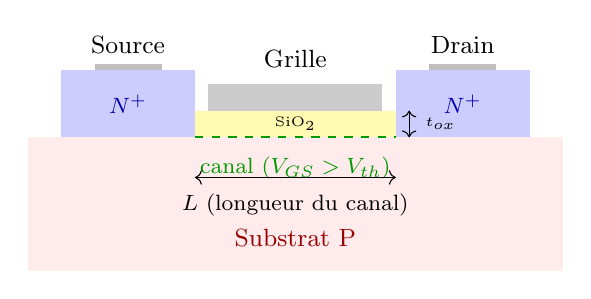
\begin{tikzpicture}[scale=0.85]
  \fill[red!8] (0,0) rectangle (8,2);
  \node[font=\small, red!60!black] at (4,0.5) {Substrat P};
  \fill[blue!20] (0.5,2) rectangle (2.5,3);
  \fill[blue!20] (5.5,2) rectangle (7.5,3);
  \node[font=\footnotesize, blue!70!black] at (1.5,2.5) {$N^+$};
  \node[font=\footnotesize, blue!70!black] at (6.5,2.5) {$N^+$};
  \node[font=\small, above] at (1.5,3.1) {Source};
  \node[font=\small, above] at (6.5,3.1) {Drain};
  \fill[gray!50] (1.0,3) rectangle (2.0,3.1);
  \fill[gray!50] (6.0,3) rectangle (7.0,3.1);
  \fill[yellow!30] (2.5,2) rectangle (5.5,2.4);
  \node[font=\tiny] at (4,2.2) {SiO$_2$};
  \fill[gray!40] (2.7,2.4) rectangle (5.3,2.8);
  \node[font=\small, above] at (4,2.9) {Grille};
  \draw[dashed, thick, green!60!black] (2.5,2) -- (5.5,2);
  \node[font=\footnotesize, green!60!black, below] at (4,1.85) {canal ($V_{GS} > V_{th}$)};
  \draw[<->, thin] (5.7,2) -- (5.7,2.4);
  \node[font=\tiny, right] at (5.8,2.2) {$t_{ox}$};
  % Longueur du canal
  \draw[<->] (2.5,1.4) -- (5.5,1.4);
  \node[font=\footnotesize, below] at (4,1.3) {$L$ (longueur du canal)};
\end{tikzpicture}
\end{center}

\begin{intuition}
\textbf{Mécanisme de création du canal :}
\begin{enumerate}[nosep]
\item $V_{GS} = 0$ : entre source ($N^+$) et drain ($N^+$), le substrat P forme deux jonctions PN en inverse $\Rightarrow$ pas de conduction (sauf courant de fuite $I_{\text{off}}$).
\item $V_{GS} > 0$ : le champ électrique de la grille repousse les trous du substrat et attire les électrons minoritaires à la surface du silicium, sous l'oxyde.
\item $V_{GS} = V_{th}$ : la concentration d'électrons en surface égale le dopage du substrat $\Rightarrow$ \textbf{inversion} : un canal N se forme, connectant source et drain.
\item $V_{GS} > V_{th}$ : le canal s'enrichit $\Rightarrow$ conductance augmente, $R_{DS,\text{on}}$ diminue.
\end{enumerate}
\end{intuition}

\subsection{Le pincement du canal et la saturation}

Quand $V_{DS}$ augmente, la tension locale le long du canal varie de $0$ (côté source) à $V_{DS}$ (côté drain). La densité de porteurs dans le canal dépend de $V_{GS} - V(x) - V_{th}$, qui diminue du côté drain.

\begin{formule}
Quand $V_{DS} = V_{GS} - V_{th}$ (appelé $V_{DS,\text{sat}}$ ou $V_{\text{ov}}$ pour \textit{overdrive}), la densité de porteurs au drain tombe à zéro : le canal est ``\textbf{pincé}'' (\textit{pinch-off}). Au-delà, les porteurs traversent cette zone de pincement par dérive dans le champ $\Rightarrow$ le courant ne dépend plus de $V_{DS}$ (en première approximation).

C'est le régime de \textbf{saturation} : $I_D$ est contrôlé par $V_{GS}$ uniquement.
\end{formule}

\subsection{Équations du courant --- modèle ``long canal''}

\begin{attention}
Les équations suivantes sont valides pour le \textbf{modèle long canal} ($L \geq \SI{1}{\micro m}$). Pour les technologies CMOS avancées ($L < \SI{100}{nm}$), des effets de canal court (saturation de vitesse, DIBL, effets quantiques) modifient significativement le comportement. Les simulateurs SPICE utilisent des modèles bien plus complexes (BSIM4, PSP).
\end{attention}

\begin{formule}
\textbf{Régime bloqué} ($V_{GS} < V_{th}$) :
\[
I_D \approx I_{\text{off}} \qquad \text{(courant sub-seuil, non nul)}
\]
En sub-seuil, $I_D$ suit une loi \textit{exponentielle} similaire au BJT : $I_D \propto e^{V_{GS}/(nV_T)}$ avec $n \approx 1{,}3$--$1{,}5$.

\textbf{Régime ohmique} ($V_{GS} > V_{th}$, $V_{DS} < V_{\text{ov}} = V_{GS}-V_{th}$) :
\[
\boxed{I_D = k_n\left[V_{\text{ov}}\,V_{DS} - \frac{V_{DS}^2}{2}\right]}
\]
Pour $V_{DS} \ll V_{\text{ov}}$ : $I_D \approx k_n V_{\text{ov}} V_{DS}$, d'où $R_{DS,\text{on}} = 1/(k_n V_{\text{ov}})$.

\textbf{Régime de saturation} ($V_{DS} \geq V_{\text{ov}}$) :
\[
\boxed{I_D = \frac{k_n}{2}\,V_{\text{ov}}^2\,(1 + \lambda V_{DS})}
\]
\begin{itemize}[nosep]
\item $k_n = \mu_n C_{ox} W/L$ : paramètre de transconductance (A/V$^2$).
\item $\mu_n$ : mobilité des électrons dans le canal ($\sim\SI{400}{cm^2/(V\cdot s)}$ en Si).
\item $C_{ox} = \varepsilon_{ox}/t_{ox}$ : capacité d'oxyde par unité de surface.
\item $\lambda$ : paramètre de modulation de longueur de canal (\textit{Channel Length Modulation}, CLM). $\lambda \sim 0{,}01$ à $\SI{0.1}{V^{-1}}$. Analogue à l'effet Early du BJT.
\end{itemize}
\end{formule}

\begin{intuition}
\textbf{Pourquoi le courant est quadratique} (et non exponentiel) :
\begin{itemize}[nosep]
\item La charge dans le canal $Q_{ch} \propto C_{ox}(V_{GS} - V_{th})$ (condensateur plan).
\item La vitesse de dérive $v_d \propto \mu E \propto \mu(V_{GS}-V_{th})/L$ (champ longitudinal moyen).
\item $I_D \propto Q_{ch} \times v_d \propto (V_{GS}-V_{th})^2$.
\end{itemize}
Conséquence directe : le $g_m$ du MOSFET est plus faible que celui du BJT à même courant, car la loi quadratique ``aplatit'' la caractéristique par rapport à l'exponentielle.
\end{intuition}

\subsection{Caractéristique $I_D(V_{DS})$}

\begin{center}
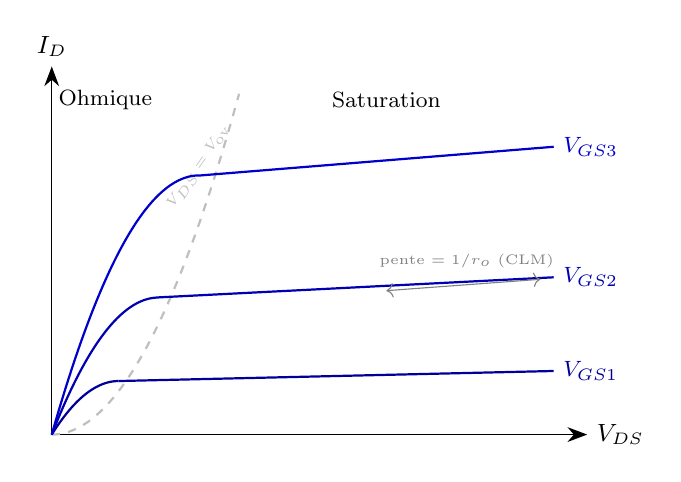
\begin{tikzpicture}[scale=0.85]
  \draw[-{Stealth[length=2.5mm]}] (0,0) -- (8,0) node[right, font=\small]{$V_{DS}$};
  \draw[-{Stealth[length=2.5mm]}] (0,0) -- (0,5.5) node[above, font=\small]{$I_D$};
  \draw[dashed, gray!50, thick, domain=0:2.8, samples=80, smooth]
    plot(\x, {0.65*\x*\x});
  \node[gray!50, font=\tiny, rotate=55] at (2.2,4) {$V_{DS} = V_{\text{ov}}$};
  % VGS1
  \draw[thick, blue!60!black, domain=0:1.0, samples=50, smooth]
    plot(\x, {0.8*(2*1*\x - \x*\x)});
  \draw[thick, blue!60!black] (1.0,0.8) -- (7.5,0.95);
  \node[right, font=\footnotesize, blue!60!black] at (7.5,0.95) {$V_{GS1}$};
  % VGS2
  \draw[thick, blue!70!black, domain=0:1.6, samples=50, smooth]
    plot(\x, {0.8*(2*1.6*\x - \x*\x)});
  \draw[thick, blue!70!black] (1.6,2.05) -- (7.5,2.35);
  \node[right, font=\footnotesize, blue!70!black] at (7.5,2.35) {$V_{GS2}$};
  % VGS3
  \draw[thick, blue!80!black, domain=0:2.2, samples=50, smooth]
    plot(\x, {0.8*(2*2.2*\x - \x*\x)});
  \draw[thick, blue!80!black] (2.2,3.87) -- (7.5,4.3);
  \node[right, font=\footnotesize, blue!80!black] at (7.5,4.3) {$V_{GS3}$};
  \node[font=\footnotesize] at (0.8,5) {Ohmique};
  \node[font=\footnotesize] at (5,5) {Saturation};
  % Pente en saturation annotée
  \draw[<->, thin, gray] (5,2.15) -- (7.3,2.32);
  \node[font=\tiny, gray, above] at (6.2,2.35) {pente $= 1/r_o$ (CLM)};
\end{tikzpicture}
\end{center}

\subsection{Modèle petit signal du MOSFET}

\subsubsection*{Transconductance $g_m$}

En saturation ($I_D = k_n V_{\text{ov}}^2/2$), on dérive par rapport à $V_{GS}$ :

\begin{formule}
\[
\boxed{g_m = \frac{\partial I_D}{\partial V_{GS}}\bigg|_Q = k_n\,V_{\text{ov}} = \frac{2I_{D,Q}}{V_{\text{ov}}} = \sqrt{2\,k_n\,I_{D,Q}}}
\]
\textbf{Trois expressions équivalentes}, chacune utile dans un contexte différent :
\begin{itemize}[nosep]
\item $k_n V_{\text{ov}}$ : pour le dimensionnement géométrique ($W/L$).
\item $2I_D/V_{\text{ov}}$ : pour raisonner en termes de rendement d'utilisation du courant.
\item $\sqrt{2k_n I_D}$ : pour comparer avec le BJT.
\end{itemize}

\textbf{Comparaison BJT vs MOSFET à $I = \SI{1}{mA}$ :}
\begin{itemize}[nosep]
\item BJT : $g_m = I_C/V_T = 1/0{,}026 = \SI{38.5}{mA/V}$.
\item MOSFET ($k_n = \SI{1}{mA/V^2}$) : $g_m = \sqrt{2\times10^{-3}\times10^{-3}} = \SI{1.41}{mA/V}$.
\end{itemize}
Le MOSFET est $\sim 27\times$ moins transconducteur à même courant. On compense par $W/L$ élevé (facile en CI) ou par un courant plus élevé.
\end{formule}

\subsubsection*{Résistance de sortie $r_o$}

\begin{formule}
\[
\boxed{r_o = \frac{1}{\lambda\,I_{D,Q}} = \frac{V_A}{I_{D,Q}}}
\]
avec $V_A = 1/\lambda$ : ``tension d'Early'' du MOSFET. Typiquement $V_A \sim \SI{10}{V}$ à \SI{50}{V} (plus faible que le BJT : \SI{50}{V}--\SI{200}{V}).
\end{formule}

\subsubsection*{Le schéma équivalent}

\begin{center}
\begin{circuitikz}[scale=1.0, american]
  \node[left, font=\small] at (0,0) {G};
  \node[right, font=\small] at (8,0) {D};
  \node[left, font=\small] at (0,-3) {S};
  \node[right, font=\small] at (8,-3) {S};
  \draw (0,0) -- (2,0);
  \draw (0,-3) -- (8,-3);
  \draw (4.5,0) to[american controlled current source, l_=$g_m\,v_{gs}$] (4.5,-3);
  \draw (2,0) -- (4.5,0);
  \draw (7,0) to[R, l=$r_o$] (7,-3);
  \draw (4.5,0) -- (7,0);
  \draw (7,0) -- (8,0);
  \filldraw (2,0) circle (1.5pt);
  \filldraw (4.5,0) circle (1.5pt);
  \filldraw (4.5,-3) circle (1.5pt);
  \filldraw (7,0) circle (1.5pt);
  \filldraw (7,-3) circle (1.5pt);
  \draw[{Stealth[length=2.5mm]}-{Stealth[length=2.5mm]}, thick] (1,-0.15) -- (1,-2.85);
  \node[font=\small, left] at (0.95,-1.5) {$v_{gs}$};
  \node[font=\tiny, red!70!black, right] at (2.1,0.25) {$i_g \approx 0$ (BF)};
\end{circuitikz}
\end{center}

\begin{intuition}
\textbf{Différence structurelle avec le BJT :} pas de $r_\pi$. La grille est un circuit ouvert en BF (impédance infinie). Le MOSFET est un pur convertisseur \textbf{tension $\to$ courant}. En HF, il faut ajouter $C_{GS}$ (entre G et S) et $C_{GD}$ (entre G et D), et l'impédance d'entrée devient $Z_G(j\omega) = 1/[j\omega(C_{GS}+C_{GD}(1+g_m R_D))]$ (effet Miller sur $C_{GD}$).
\end{intuition}

% ============================================================================
\section{Niveau Ingénieur}

\begin{ingenieur}
$R_{DS,\text{on}}$ et ses dépendances, capacités parasites et plateau de Miller, pertes de commutation (énergie vs puissance), CMOS, bruit, effets thermiques, et technologies avancées (GaN, SiC).
\end{ingenieur}

\subsection{$R_{DS,\text{on}}$ : le paramètre clé en puissance}

\begin{formule}
$R_{DS,\text{on}}$ dépend de trois facteurs indépendants :
\begin{itemize}[nosep]
\item \textbf{$V_{GS}$} : plus $V_{GS} \gg V_{th}$, plus le canal est conducteur, plus $R_{DS,\text{on}}$ est faible. Les datasheets spécifient $R_{DS,\text{on}}$ pour un $V_{GS}$ donné (typiquement \SI{10}{V} ou \SI{4.5}{V} pour les MOSFETs ``logic level'').
\item \textbf{Température} : $R_{DS,\text{on}}$ \textbf{augmente} avec $T$ ($+0{,}3\%/°$C à $+0{,}8\%/°$C) car la mobilité $\mu$ diminue ($\mu \propto T^{-1{,}5}$ à $T^{-2{,}5}$). C'est stabilisant (pas d'emballement), mais la puissance dissipée augmente quand le composant chauffe.
\item \textbf{$V_{DS,\max}$} : le compromis fondamental ``on-resistance vs breakdown voltage''. La zone de drift (N faiblement dopé entre canal et drain) doit être plus longue et moins dopée pour tenir une haute tension $\Rightarrow$ $R_{DS,\text{on}} \propto V_{BR}^{2{,}5}$ (loi de Baliga). Les MOSFETs haute tension ($\SI{600}{V}$+) ont des $R_{DS,\text{on}}$ 100 à 1000$\times$ plus élevés que les basse tension (\SI{30}{V}).
\end{itemize}
\end{formule}

\begin{pratique}
\begin{center}
\begin{tabular}{lll}
\toprule
\textbf{$V_{DS,\max}$} & \textbf{$R_{DS,\text{on}}$ typique} & \textbf{Application} \\
\midrule
\SI{30}{V} & \SI{1}{m\ohm}--\SI{10}{m\ohm} & DC-DC basse tension (VRM, PoL) \\
\SI{100}{V} & \SI{5}{m\ohm}--\SI{50}{m\ohm} & Alimentation 48V, moteurs \\
\SI{600}{V} & \SI{50}{m\ohm}--\SI{500}{m\ohm} & Onduleur secteur, PFC \\
\bottomrule
\end{tabular}
\end{center}
\end{pratique}

\subsection{Capacités parasites et plateau de Miller}

\begin{formule}
\textbf{Les trois capacités :}
\begin{itemize}[nosep]
\item $C_{GS}$ : capacité grille-source. Quasi constante. Domine $C_{iss}$.
\item $C_{GD}$ : capacité grille-drain. \textbf{Fortement non-linéaire} : chute brutalement quand $V_{DS}$ augmente (la zone de déplétion s'élargit côté drain). C'est la capacité la plus critique en commutation.
\item $C_{DS}$ : capacité drain-source. Non-linéaire aussi.
\end{itemize}
Notation datasheet : $C_{iss} = C_{GS}+C_{GD}$, $C_{oss} = C_{DS}+C_{GD}$, $C_{rss} = C_{GD}$.
\end{formule}

\subsubsection*{Le plateau de Miller}

Lors de la commutation ON, la tension de grille $V_{GS}$ ne monte pas linéairement. Elle présente un \textbf{plateau} à $V_{GS} \approx V_{th} + I_D/g_m$ pendant lequel \textit{toute} l'énergie du driver charge $C_{GD}$ pour faire chuter $V_{DS}$. Pendant ce plateau, $V_{GS}$ est quasi constante :

\begin{intuition}
\textbf{Chronologie d'une commutation ON :}
\begin{enumerate}[nosep]
\item \textbf{Phase 1 :} $V_{GS}$ monte de $0$ à $V_{th}$. Le MOSFET est bloqué. On charge $C_{GS}+C_{GD}$.
\item \textbf{Phase 2 :} $V_{GS}$ dépasse $V_{th}$, $I_D$ croît. $V_{DS}$ commence à chuter. Pertes de commutation élevées ($V_{DS}$ et $I_D$ non nuls simultanément).
\item \textbf{Phase 3 (plateau de Miller) :} $V_{GS} \approx$ constante. Le courant du driver charge $C_{GD}$ pour faire chuter $V_{DS}$. \textbf{Plus $C_{GD}$ est grand, plus cette phase est longue et dissipative.}
\item \textbf{Phase 4 :} $V_{DS} \approx R_{DS,\text{on}} I_D$. $V_{GS}$ reprend sa montée. Le MOSFET est pleinement en conduction.
\end{enumerate}
C'est pourquoi les drivers de grille doivent fournir un courant \textit{élevé} (plusieurs ampères) pour traverser le plateau de Miller rapidement et minimiser les pertes.
\end{intuition}

\subsection{Pertes de commutation : énergie vs puissance}

\begin{formule}
\textbf{Énergie dissipée par événement de commutation} (approximation linéaire) :
\[
E_{\text{on}} \approx \frac{1}{2}V_{DS}\,I_D\,t_{\text{on}} \qquad E_{\text{off}} \approx \frac{1}{2}V_{DS}\,I_D\,t_{\text{off}}
\]

\textbf{Puissance moyenne de commutation} :
\[
\boxed{P_{sw} = (E_{\text{on}} + E_{\text{off}}) \cdot f_{sw} = \frac{1}{2}V_{DS}\,I_D\,(t_{\text{on}}+t_{\text{off}})\,f_{sw}}
\]

\textbf{Pertes totales} :
\[
\boxed{P_{\text{total}} = \underbrace{R_{DS,\text{on}} \cdot I_D^2 \cdot D}_{\text{conduction}} + \underbrace{(E_{\text{on}}+E_{\text{off}})\cdot f_{sw}}_{\text{commutation}} + \underbrace{\frac{1}{2}C_{oss}\,V_{DS}^2\,f_{sw}}_{\text{capacitives}}}
\]
Le terme capacitif ($C_{oss}$) devient significatif à haute fréquence et haute tension.
\end{formule}

\subsection{Bruit dans le MOSFET}

\begin{formule}
\begin{itemize}[nosep]
\item \textbf{Bruit thermique du canal} : $\overline{i_d^2} = 4kT\gamma g_m \Delta f$ avec $\gamma \approx 2/3$ (long canal) à $\gamma \approx 1$--$2$ (canal court).
\item \textbf{Bruit $1/f$ (flicker)} : $\overline{v_g^2} = \dfrac{K_F}{C_{ox}WL}\cdot\dfrac{\Delta f}{f}$. Proportionnel à $1/(WL)$ : \textbf{plus le transistor est grand, moins il est bruyant} en $1/f$. Ce bruit est plus élevé que dans le BJT car les porteurs circulent à l'\textit{interface} Si/SiO$_2$, riche en pièges.
\end{itemize}

\textbf{Conséquence pour la conception :} en audio/instrumentation basse fréquence, le BJT est souvent préféré (faible $1/f$). En RF, le MOSFET peut être compétitif si $W/L$ est grand (dilue le bruit $1/f$), ou si la fréquence est assez haute pour que le bruit thermique domine.
\end{formule}

\subsection{Effets thermiques}

\begin{formule}
Trois paramètres varient avec la température :
\begin{itemize}[nosep]
\item $\mu$ \textbf{diminue} ($\propto T^{-1{,}5}$ à $T^{-2{,}5}$) $\Rightarrow$ $g_m \downarrow$ et $R_{DS,\text{on}} \uparrow$ (\textbf{stabilisant}).
\item $V_{th}$ \textbf{diminue} ($\approx \SI{-2}{mV/°C}$ à $\SI{-5}{mV/°C}$) $\Rightarrow$ le MOSFET conduit à un $V_{GS}$ plus faible. En logique, cela peut créer des problèmes de marges de bruit à haute température.
\item $I_{\text{off}}$ (courant de fuite sub-seuil) \textbf{augmente} exponentiellement ($\sim\times 2$ tous les \SI{10}{°C}). Dans les SoC modernes ($L < \SI{10}{nm}$), les fuites à chaud deviennent un problème de consommation majeur.
\end{itemize}
\textbf{Point de croisement ZTC} (\textit{Zero Temperature Coefficient}) : il existe un $V_{GS}$ pour lequel les effets de $\mu \downarrow$ et $V_{th} \downarrow$ se compensent exactement, rendant $I_D$ indépendant de $T$. Ce point est utilisé pour les références de courant.
\end{formule}

\subsection{L'inverseur CMOS}

\begin{center}
\begin{circuitikz}[scale=0.9, american]
  \draw (2,5) node[above]{$V_{DD}$} -- (2,4.5);
  \draw (2,4.5) -- (2,4);
  \draw (0.5,3.2) node[pmos, anchor=G](MP){};
  \draw (MP.S) -- (2,4);
  \draw (MP.D) -- (2,2);
  \draw (0.5,1) node[nmos, anchor=G](MN){};
  \draw (MN.D) -- (2,2);
  \draw (MN.S) -- (2,-0.5) node[ground]{};
  \draw (MP.G) -- (MN.G);
  \draw (MP.G) -- ++(-1,0) node[left]{$V_{\text{in}}$};
  \draw (2,2) -- ++(1.5,0) node[right]{$V_{\text{out}}$};
  \filldraw (2,2) circle (1.5pt);
\end{circuitikz}
\end{center}

\begin{formule}
\textbf{Puissance dynamique CMOS :}
\[
\boxed{P_{\text{dyn}} = \alpha \cdot C_L \cdot V_{DD}^2 \cdot f}
\]
avec $\alpha$ le facteur d'activité ($0{,}1$ à $0{,}3$ typique). \textbf{Puissance statique} (fuites) : $P_{\text{stat}} = V_{DD} \cdot I_{\text{off}} \cdot N$, croissante avec $T$ et la réduction de $L$.
\end{formule}

\subsection{Technologies avancées}

\begin{pratique}
\begin{itemize}[nosep]
\item \textbf{GaN} (nitrure de gallium) : mobilité élevée, champ critique $10\times$ supérieur au Si $\Rightarrow$ $R_{DS,\text{on}}$ très faible à haute tension, capacités parasites réduites. Commutation à \SI{1}{MHz}--\SI{10}{MHz}. Rendements $> 99\%$ dans les chargeurs et serveurs.
\item \textbf{SiC} (carbure de silicium) : champ critique $10\times$ Si, excellente tenue en température ($T_j > \SI{200}{°C}$). Dominance en haute tension ($> \SI{600}{V}$) et haute température (véhicules électriques, photovoltaïque, traction).
\item \textbf{CMOS avancé} ($L < \SI{10}{nm}$) : effets de canal court (DIBL, SCE), FinFET et GAA (Gate-All-Around) pour maintenir le contrôle électrostatique, tensions d'alimentation $< \SI{0.8}{V}$, fuites dominantes.
\end{itemize}
\end{pratique}

% === EXERCICES ===
\section*{Exercices}
\addcontentsline{toc}{section}{Exercices}

\subsection*{Niveau débutant}

\textbf{Exercice 17.1 ---} NMOS, $V_{th} = \SI{2}{V}$, $V_{DS} = \SI{3}{V}$. Déterminez le régime pour $V_{GS} = \SI{5}{V}$ et $V_{GS} = \SI{1}{V}$.

\begin{pratique}
\textbf{Solution :} $V_{GS} = 5$ : $V_{\text{ov}} = 3$, $V_{DS} = 3 = V_{\text{ov}}$ $\Rightarrow$ frontière saturation/ohmique ($\geq$ : saturation).

$V_{GS} = 1 < V_{th}$ $\Rightarrow$ bloqué ($I_D \approx I_{\text{off}}$, pas exactement nul).
\end{pratique}

\textbf{Exercice 17.2 ---} MOSFET ($R_{DS,\text{on}} = \SI{10}{m\ohm}$) vs BJT ($V_{CE,\text{sat}} = \SI{0.2}{V}$) pour commuter \SI{5}{A}. Comparez les pertes.

\begin{pratique}
\textbf{Solution :} MOSFET : $P = 0{,}01\times25 = \SI{250}{mW}$. BJT : $P = 0{,}2\times5 = \SI{1}{W}$. Le MOSFET dissipe $4\times$ moins. De plus, le BJT nécessite $I_B \approx \SI{50}{mA}$ en permanence.
\end{pratique}

\subsection*{Niveau intermédiaire}

\textbf{Exercice 17.3 ---} NMOS ($k_n = \SI{2}{mA/V^2}$, $V_{th} = \SI{1.5}{V}$, $\lambda = \SI{0.02}{V^{-1}}$), $V_{GS} = \SI{3}{V}$, $R_D = \SI{5}{k\ohm}$. Calculez $I_D$, $g_m$, $r_o$, $A_v$.

\begin{pratique}
\textbf{Solution :} $V_{\text{ov}} = 1{,}5$. $I_D = 10^{-3}\times2{,}25 = \SI{2.25}{mA}$. $g_m = 2\times10^{-3}\times1{,}5 = \SI{3}{mA/V}$. $r_o = 1/(0{,}02\times2{,}25\times10^{-3}) = \SI{22.2}{k\ohm}$.

$A_v = -g_m(R_D\parallel r_o) = -3\times10^{-3}\times(5000\parallel22200) = -3\times10^{-3}\times4080 = -12{,}2$.
\end{pratique}

\textbf{Exercice 17.4 ---} Buck : $V_{\text{in}} = \SI{24}{V}$, $V_{\text{out}} = \SI{5}{V}$, $I_L = \SI{10}{A}$, $f_{sw} = \SI{500}{kHz}$, $R_{DS,\text{on}} = \SI{5}{m\ohm}$, $t_r = t_f = \SI{20}{ns}$. Calculez les pertes en conduction et commutation. Lequel domine ?

\begin{pratique}
\textbf{Solution :} $D = 5/24 = 0{,}208$. $P_{\text{cond}} = 0{,}005\times100\times0{,}208 = \SI{104}{mW}$.

$E_{\text{on}}+E_{\text{off}} = V_{\text{in}}\times I_L\times(t_r+t_f)/2 = 24\times10\times40\times10^{-9}/2 = \SI{4.8}{\micro J}$.

$P_{sw} = 4{,}8\times10^{-6}\times500\times10^3 = \SI{2.4}{W}$.

Les pertes de commutation (\SI{2.4}{W}) dominent largement les pertes de conduction (\SI{104}{mW}) --- facteur $23\times$. C'est typique à haute fréquence.
\end{pratique}

\subsection*{Niveau ingénieur}

\textbf{Exercice 17.5 ---} Inverseur CMOS ($k_n = \SI{200}{\micro A/V^2}$, $k_p = \SI{100}{\micro A/V^2}$, $V_{DD} = \SI{1.8}{V}$, $C_L = \SI{50}{fF}$, $f = \SI{1}{GHz}$, $\alpha = 0{,}1$). Calculez $W_P/W_N$ pour la symétrie et la puissance dynamique.

\begin{pratique}
\textbf{Solution :} $W_P/W_N = k_n/k_p = 200/100 = 2$ (compense $\mu_p < \mu_n$).

$P_{\text{dyn}} = \alpha C_L V_{DD}^2 f = 0{,}1\times50\times10^{-15}\times3{,}24\times10^9 = \SI{16.2}{\micro W}$ par porte.
\end{pratique}

\textbf{Exercice 17.6 ---} NMOS ($k_n = \SI{5}{mA/V^2}$, $V_{th} = \SI{1}{V}$, $\lambda = \SI{0.02}{V^{-1}}$) en source commune, $R_D = \SI{2}{k\ohm}$, $V_{DD} = \SI{10}{V}$, $V_{GS,Q} = \SI{2.5}{V}$. Le point de repos est-il en saturation ?

\begin{pratique}
\textbf{Solution :} $V_{\text{ov}} = 1{,}5$. $I_D \approx 5\times10^{-3}\times2{,}25/2 = \SI{5.625}{mA}$. $V_{DS} = 10 - 5{,}625\times2 = \SI{-1.25}{V}$ : \textbf{impossible} ($V_{DS} < 0$). Le MOSFET est en \textbf{triode}, pas en saturation.

$V_{GS,Q} = \SI{2}{V}$ : $V_{\text{ov}} = 1$. $I_D = 2{,}5\times1/2 = \SI{2.5}{mA}$. $V_{DS} = 10-5 = \SI{5}{V} > V_{\text{ov}}$ : saturation confirmée.

$g_m = \SI{5}{mA/V}$. $r_o = 1/(0{,}02\times2{,}5\times10^{-3}) = \SI{20}{k\ohm}$. $A_v = -5\times10^{-3}\times(2000\parallel20000) = -9{,}1$.
\end{pratique}

\subsection*{Questions de compréhension}

\begin{enumerate}[nosep]
\item Pourquoi le MOSFET est-il thermiquement stable alors que le BJT ne l'est pas ? Quel paramètre physique ($\mu$ vs $I_S$) est responsable ?
\item Pourquoi le bruit $1/f$ du MOSFET est-il plus élevé que celui du BJT ? Quel paramètre de conception réduit ce bruit ?
\item Expliquez physiquement le plateau de Miller lors d'une commutation ON. Pourquoi $V_{GS}$ reste-t-il quasi constant pendant que $V_{DS}$ chute ?
\item Pourquoi $R_{DS,\text{on}} \propto V_{BR}^{2{,}5}$ (loi de Baliga) ? Qu'est-ce que le GaN change à cette relation ?
\end{enumerate}

% === RÉSUMÉ ===
\section*{Résumé du chapitre}
\addcontentsline{toc}{section}{Résumé du chapitre}

\begin{bases}[title={\color{white} Résumé --- Les Bases}]
\begin{center}
\renewcommand{\arraystretch}{1.3}
\begin{tabular}{p{3.5cm}p{9.5cm}}
\toprule
Commande & Tension $V_{GS}$, courant $\approx 0$ en statique (capacitif en dynamique) \\
3 régimes & Bloqué ($I_D \approx I_{\text{off}}$), ohmique ($R_{DS,\text{on}}$), saturation (source de courant) \\
Commutation & $P = R_{DS,\text{on}} I_D^2$ --- minimiser $R_{DS,\text{on}}$ \\
Thermique & $R_{DS,\text{on}} \uparrow$ avec $T$ $\Rightarrow$ auto-stable \\
Piège & Saturation MOSFET $\neq$ saturation BJT \\
\bottomrule
\end{tabular}
\end{center}
\end{bases}

\begin{approfondissement}[title={\color{white} Résumé --- Approfondissement}]
\begin{center}
\renewcommand{\arraystretch}{1.3}
\begin{tabular}{p{3.5cm}p{9.5cm}}
\toprule
Saturation & $I_D = k_n V_{\text{ov}}^2/2\,(1+\lambda V_{DS})$ --- loi quadratique (long canal) \\
Pinch-off & Canal pincé à $V_{DS} = V_{\text{ov}}$ $\Rightarrow$ $I_D$ indépendant de $V_{DS}$ \\
$g_m$ (au point $Q$) & $k_n V_{\text{ov}} = 2I_D/V_{\text{ov}} = \sqrt{2k_n I_D}$ --- $\ll g_m$ du BJT \\
$r_o$ (CLM) & $1/(\lambda I_D) = V_A/I_D$ \\
Modèle petit signal & Source $g_m v_{gs}$ + $r_o$, \textbf{pas de $r_\pi$} \\
\bottomrule
\end{tabular}
\end{center}
\end{approfondissement}

\begin{ingenieur}[title={\color{white} Résumé --- Niveau Ingénieur}]
\begin{center}
\renewcommand{\arraystretch}{1.3}
\begin{tabular}{p{3.5cm}p{9.5cm}}
\toprule
$R_{DS,\text{on}}$ & $\propto V_{BR}^{2{,}5}$ (Baliga), augmente avec $T$ \\
Capacités & $C_{GS}$, $C_{GD}$ (Miller, non-linéaire), $C_{DS}$ \\
Plateau Miller & Phase à $V_{GS}$ constante pendant laquelle $V_{DS}$ chute \\
Pertes & Conduction ($RI^2D$) + commutation ($EfN$) + capacitives \\
Bruit & Thermique ($4kT\gamma g_m$) + $1/f$ ($K_F/(C_{ox}WLf)$) \\
GaN / SiC & Champ critique $10\times$ Si, $f_{sw} > \SI{1}{MHz}$, $T_j > \SI{200}{°C}$ \\
\bottomrule
\end{tabular}
\end{center}
\end{ingenieur}

% ============================================================================
% CHAPITRE 18 : L'AMPLIFICATEUR OPÉRATIONNEL — VERSION PEER-REVIEW
% ============================================================================
% ============================================================================
% CHAPITRE 18 : L'AMPLIFICATEUR OPÉRATIONNEL (AOP)
% VERSION AUGMENTÉE — peer-review + pédagogie
% Fichier autonome à intégrer dans Bible_Elec.tex
% ============================================================================

\chapter{L'Amplificateur Opérationnel (AOP)}

\begin{center}
\textit{L'amplificateur opérationnel est le composant central\\
de l'électronique analogique. Avec deux résistances et un AOP,\\
on réalise un amplificateur de précision dont le gain ne dépend\\
que du rapport de résistances --- pas des transistors internes.\\
C'est la puissance de la rétroaction négative.}
\end{center}

\vspace{0.5cm}

Un amplificateur opérationnel (AOP ou \textit{op-amp}) est un \textbf{amplificateur différentiel à très fort gain}. Utilisé avec une \textbf{rétroaction négative}, il devient un outil universel : amplificateur, sommateur, intégrateur, filtre actif, comparateur, convertisseur\ldots Pratiquement tout circuit analogique en contient.

Ce chapitre commence par les outils pratiques (comment résoudre un circuit à AOP), puis explique d'où viennent les propriétés de l'AOP en le reliant aux transistors des chapitres 16 et 17, et termine par les limites réelles qui contraignent la conception.

\begin{intuition}
\textbf{Ce que nous allons expliquer dans ce chapitre :}
\begin{itemize}[nosep]
\item Pourquoi le gain de l'AOP est très élevé \textit{mais pas infini} (il vient de $g_m \times r_o$ des transistors internes).
\item Pourquoi la rétroaction négative transforme un composant instable en amplificateur précis.
\item Pourquoi la bande passante est limitée (capacités parasites, effet Miller).
\item Ce qu'est le slew rate et pourquoi c'est une limitation en \textit{courant}, pas en fréquence.
\item Pourquoi le choix de la technologie d'entrée (BJT, JFET, CMOS) dépend de l'application.
\item Comment la stabilité et le bruit contraignent la conception.
\end{itemize}
\end{intuition}

% ============================================================================
\section{Les Bases}

\begin{bases}
Outils pratiques pour résoudre les circuits à AOP : règles d'or, méthode de résolution, montages fondamentaux, et limites de validité. Prérequis : chapitres 1 à 6 (KCL, KVL, Thévenin).
\end{bases}

\subsection{Qu'est-ce qu'un AOP ?}

Un AOP possède deux entrées et une sortie :

\begin{center}
\begin{circuitikz}[scale=1.0, american]
  \draw (0,0) node[op amp, thick](AOP){};
  \node[left, font=\small] at (AOP.+) {$V^+$};
  \node[left, font=\small] at (AOP.-) {$V^-$};
  \draw (AOP.out) -- ++(0.8,0) node[right, font=\small]{$V_{\text{out}}$};
  \draw (AOP.up) -- ++(0,0.4) node[above, font=\footnotesize]{$+V_{CC}$};
  \draw (AOP.down) -- ++(0,-0.4) node[below, font=\footnotesize]{$-V_{EE}$};
\end{circuitikz}
\end{center}

\begin{formule}
\textbf{Relation fondamentale :}
\[
\boxed{V_{\text{out}} = A_{OL} \cdot (V^+ - V^-)}\]
$A_{OL}$ : gain en \textbf{boucle ouverte} (\textit{open loop}). Typiquement $10^5$ à $10^6$ ($\SI{100}{dB}$ à $\SI{120}{dB}$) en DC. Ce gain est très élevé mais \textbf{fini}. Il diminue avec la fréquence.
\end{formule}

\begin{intuition}
\textbf{Le rôle de la rétroaction :} un gain de $10^5$ est inutilisable directement (la moindre tension d'entrée de $\SI{0.1}{mV}$ donne $\SI{10}{V}$ en sortie --- saturation immédiate). On utilise donc une \textbf{rétroaction négative} : une fraction de la sortie est renvoyée sur l'entrée inverseuse pour ``calmer'' le gain et le fixer à une valeur précise, déterminée par les résistances du circuit.
\end{intuition}

\subsection{Les ``règles d'or'' pour résoudre les circuits}

Quand l'AOP est en rétroaction négative et que $A_{OL}$ est suffisamment grand :

\begin{formule}
\textbf{Règle 1 :} $\boxed{V^+ = V^-}$ \quad (la tension différentielle est $\approx 0$).

\textbf{Règle 2 :} $\boxed{I^+ = 0 \text{ et } I^- = 0}$ \quad (aucun courant n'entre dans les entrées de l'AOP).

Ces deux règles, combinées aux lois de Kirchhoff, suffisent à résoudre \textbf{tout circuit AOP en régime linéaire}.
\end{formule}

% ========= BLOC MÉTHODE =========
\subsection{Méthode universelle de résolution}

\begin{pratique}
\textbf{Algorithme en 6 étapes pour résoudre tout circuit AOP :}

\textbf{Étape 1 --- Vérifier la rétroaction négative.}

Y a-t-il un chemin de la sortie vers l'entrée \textbf{inverseuse} ($V^-$) ? Si oui : l'AOP est en régime linéaire, les règles d'or s'appliquent. Si non (retour sur $V^+$ ou pas de retour) : comparateur ou oscillateur, les règles d'or ne s'appliquent \textbf{pas}.

\textbf{Étape 2 --- Appliquer la règle 1 : $V^+ = V^-$.}

Écrire l'égalité entre les potentiels des deux entrées.

\textbf{Étape 3 --- Identifier les potentiels connus.}

Quels potentiels sont fixés par le circuit ? $V_{\text{in}}$, la masse, $V_{\text{ref}}$\ldots

\textbf{Étape 4 --- Appliquer la loi des n\oe uds (KCL) au point $V^-$.}

Grâce à la règle 2 ($I^- = 0$), tout le courant qui arrive au n\oe ud $V^-$ par les résistances doit en repartir par les résistances. L'AOP ne ``consomme'' rien.

\textbf{Étape 5 --- Isoler $V_{\text{out}}$.}

Résoudre le système d'équations pour exprimer $V_{\text{out}}$ en fonction de $V_{\text{in}}$ et des résistances.

\textbf{Étape 6 --- Vérifier la cohérence.}

Le résultat $V_{\text{out}}$ est-il entre $-V_{EE}$ et $+V_{CC}$ ? Si non : la sortie est \textbf{saturée} et les règles d'or sont invalidées.
\end{pratique}

% ========= EXEMPLE GUIDÉ =========
\subsection{Exemple guidé complet : le non-inverseur}

Appliquons la méthode sur l'amplificateur non-inverseur, en trois niveaux de complexité croissante.

\begin{center}
\begin{circuitikz}[scale=0.85, american]
  \draw (0,0) node[op amp](AOP){};
  \draw (AOP.+) -- ++(-1,0) node[left]{$V_{\text{in}}$};
  \draw (AOP.out) -- ++(0.8,0) node[right]{$V_{\text{out}}$};
  \draw (AOP.out) -- ++(0.5,0) -- ++(0,-1.8) coordinate(FB);
  \draw (FB) to[R, l=$R_2$] ++(-2.5,0) coordinate(J);
  \draw (J) to[R, l=$R_1$] ++(0,-1.5) node[ground]{};
  \draw (J) -- (J |- AOP.-) -- (AOP.-);
  \filldraw (J) circle (1.5pt);
\end{circuitikz}
\end{center}

\subsubsection*{Niveau 1 : calcul avec les règles d'or}

\begin{pratique}
\textbf{Étape 1 :} la sortie est reliée à $V^-$ via $R_2$ $\Rightarrow$ rétroaction négative. \checkmark

\textbf{Étape 2 :} $V^+ = V^-$. Or $V^+ = V_{\text{in}}$, donc $V^- = V_{\text{in}}$.

\textbf{Étape 3 :} $V_{\text{in}}$ est connu. La borne basse de $R_1$ est à la masse ($0$\,V).

\textbf{Étape 4 :} KCL au n\oe ud $V^-$. Courant dans $R_1$ : $I_1 = V^-/R_1 = V_{\text{in}}/R_1$ (descendant). Courant dans $R_2$ : $I_2 = (V_{\text{out}} - V^-)/R_2 = (V_{\text{out}} - V_{\text{in}})/R_2$ (venant de la sortie). Comme $I^- = 0$ : $I_1 = I_2$.
\[
\frac{V_{\text{in}}}{R_1} = \frac{V_{\text{out}} - V_{\text{in}}}{R_2}
\]

\textbf{Étape 5 :} $V_{\text{in}} R_2 = R_1 (V_{\text{out}} - V_{\text{in}})$ $\Rightarrow$ $V_{\text{out}} = V_{\text{in}}\left(1 + \dfrac{R_2}{R_1}\right)$.

\[
\boxed{A_{CL} = 1 + \frac{R_2}{R_1}}
\]

\textbf{Étape 6 :} avec $R_1 = \SI{1}{k\ohm}$, $R_2 = \SI{9}{k\ohm}$, $V_{\text{in}} = \SI{1}{V}$ : $V_{\text{out}} = 10\times1 = \SI{10}{V}$. Si l'alimentation est $\pm\SI{15}{V}$ : $\SI{10}{V} < \SI{15}{V}$, pas de saturation. \checkmark
\end{pratique}

\subsubsection*{Niveau 2 : correction avec $A_{OL}$ fini}

\begin{pratique}
En réalité, $V^+ \neq V^-$ exactement. Il reste $V_d = V_{\text{out}}/A_{OL}$.

Le gain réel est :
\[
A_{CL,\text{réel}} = \frac{A_{OL}}{1 + A_{OL}\,\beta} = \frac{A_{OL}}{1 + A_{OL}\,\frac{R_1}{R_1+R_2}}
\]

Avec $A_{CL} = 10$ et $A_{OL} = 10\,000$ ($\SI{80}{dB}$) :

$\beta = R_1/(R_1+R_2) = 1/10$. $A_{CL,\text{réel}} = 10000/(1+10000\times0{,}1) = 10000/1001 = 9{,}990$.

Erreur : $(10 - 9{,}990)/10 = 0{,}1\%$. Acceptable pour la plupart des applications.

Si $A_{OL}$ tombe à $100$ (par exemple à haute fréquence) : $A_{CL,\text{réel}} = 100/11 = 9{,}09$. Erreur : $9{,}1\%$. \textbf{Les règles d'or ne sont plus valables.}
\end{pratique}

\subsubsection*{Niveau 3 : limites réelles}

\begin{pratique}
\begin{itemize}[nosep]
\item \textbf{Bande passante :} si $GBW = \SI{1}{MHz}$, la bande passante en BF est $f_{BW} = GBW/A_{CL} = 10^6/10 = \SI{100}{kHz}$. Au-delà, le gain chute.
\item \textbf{Slew rate :} si $SR = \SI{0.5}{V/\micro s}$, la sortie ne peut varier que de $\SI{0.5}{V}$ par $\mu$s. Pour un signal de $\SI{10}{V}$ crête, la fréquence max est $SR/(2\pi V_p) = \SI{8}{kHz}$. C'est la limite \textit{grand signal}, bien en dessous du $\SI{100}{kHz}$ petit signal.
\item \textbf{Saturation :} si $V_{\text{in}} = \SI{2}{V}$ et $A_{CL} = 10$ : $V_{\text{out}} = \SI{20}{V}$. Mais si l'alimentation est $\pm\SI{15}{V}$, la sortie sature à $\sim\SI{13}{V}$. Les règles d'or sont \textbf{invalidées}.
\end{itemize}
\end{pratique}

\subsection{Les montages fondamentaux}

\textbf{Amplificateur inverseur :}

\begin{center}
\begin{circuitikz}[scale=0.85, american]
  \draw (0,0) node[op amp](AOP){};
  \draw (AOP.+) -- ++(-0.5,0) node[ground]{};
  \draw (AOP.-) -- ++(-0.3,0) coordinate(J);
  \draw (J) to[R, l=$R_1$] ++(-2.5,0) node[left]{$V_{\text{in}}$};
  \draw (AOP.out) -- ++(0.5,0) coordinate(OUT);
  \draw (OUT) node[right]{$V_{\text{out}}$};
  \draw (J) -- ++(0,1.2) coordinate(FB);
  \draw (FB) to[R, l=$R_2$] (FB -| OUT);
  \draw (FB -| OUT) -- (OUT);
  \filldraw (J) circle (1.5pt);
  \filldraw (OUT) circle (1.5pt);
\end{circuitikz}
\end{center}

\begin{formule}
\[
\boxed{A_{CL} = -\frac{R_2}{R_1}} \qquad \text{(valable si } A_{OL} \gg |A_{CL}|\text{)}
\]
Le signe $-$ indique une \textbf{inversion de phase}. Le point $V^-$ est une ``masse virtuelle'' : il est au même potentiel que $V^+$ (= masse), mais ce n'est \textbf{pas} la masse physique (aucun courant ne s'y écoule vers la masse).
\end{formule}

\textbf{Suiveur (buffer) :} sortie directement rebouclée sur $V^-$, $R_1 \to \infty$, $R_2 = 0$ $\Rightarrow$ $A_{CL} = 1$. Impédance d'entrée $\approx \infty$, impédance de sortie $\approx 0$. C'est l'adaptation d'impédance universelle.

\textbf{Sommateur inverseur :}
\[
V_{\text{out}} = -\left(\frac{R_f}{R_1}V_1 + \frac{R_f}{R_2}V_2 + \cdots\right)
\]

\textbf{Amplificateur différentiel :}
\[
V_{\text{out}} = \frac{R_2}{R_1}(V_2 - V_1) \qquad \text{(si les résistances sont appariées)}
\]

% ========= CHECKLIST VALIDITÉ =========
\subsection{Quand les règles d'or ne sont plus valables}

\begin{attention}
\textbf{Checklist de validité --- avant de faire confiance aux règles d'or, vérifiez :}

\textbf{1. La rétroaction est-elle bien négative ?}

Si le retour va sur $V^+$ au lieu de $V^-$, c'est une rétroaction \textit{positive} : l'AOP est en comparateur ou en oscillateur. Les règles d'or ne s'appliquent pas.

\textbf{2. Le gain de boucle est-il suffisant ?}

Les règles d'or supposent $A_{OL} \gg A_{CL}$. À haute fréquence, $A_{OL}$ diminue ($-\SI{20}{dB/déc}$). Quand $A_{OL}$ devient comparable à $A_{CL}$, l'erreur de gain dépasse $1\%$ et les règles d'or perdent leur précision. Comparez toujours la fréquence de travail avec $GBW/A_{CL}$.

\textbf{3. La sortie est-elle saturée ?}

Si $V_{\text{out}}$ calculé dépasse $\pm(V_{CC} - V_{\text{headroom}})$, la sortie est bloquée contre un rail. $V^+ \neq V^-$, les règles d'or sont \textbf{fausses}. Vérifiez toujours la cohérence.

\textbf{4. Les impédances sont-elles raisonnables ?}

Si l'impédance source $> \SI{100}{k\ohm}$ (AOP BJT) ou $> \SI{10}{G\ohm}$ (AOP CMOS), le courant de polarisation $I_B$ crée une erreur d'offset significative. La règle $I^{\pm} = 0$ n'est plus assez précise.
\end{attention}

\begin{retenir}
\textbf{L'essentiel sur l'AOP :}
\begin{enumerate}[nosep]
\item L'AOP amplifie la \textbf{différence} $V^+ - V^-$ avec un gain $A_{OL}$ très élevé (mais fini).
\item Avec rétroaction négative : $V^+ \approx V^-$ et le gain est fixé par les résistances.
\item La méthode de résolution : vérifier la rétroaction $\to$ $V^+ = V^-$ $\to$ KCL au n\oe ud $V^-$ $\to$ isoler $V_{\text{out}}$ $\to$ vérifier cohérence.
\item Les règles d'or sont des \textbf{approximations}. Elles sont invalidées par la saturation, la haute fréquence, ou l'absence de rétroaction négative.
\end{enumerate}
\end{retenir}

% ============================================================================
\section{Approfondissement}

\vspace{0.3cm}
\textit{Nous quittons maintenant le monde idéal. Les sections qui suivent expliquent \textbf{d'où viennent} les propriétés de l'AOP (gain, bande passante, slew rate) en le décomposant en ses transistors internes --- ceux des chapitres 16 et 17. Chaque limitation a une cause physique précise, et la comprendre permet de choisir le bon AOP et de ne pas tomber dans les pièges classiques.}
\vspace{0.3cm}

\begin{approfondissement}
Architecture interne, origine physique du gain $A_{OL}$, théorie de la rétroaction, produit gain-bande, compensation de Miller, et slew rate. Prérequis : chapitres 16 et 17 ($g_m$, $r_o$, effet Miller).
\end{approfondissement}

\subsection{Architecture interne : d'où vient le gain ?}

L'AOP n'est \textbf{pas un composant fondamental} comme le transistor. C'est une \textbf{architecture de circuit} composée de transistors. Un AOP typique comprend trois étages :

\begin{center}
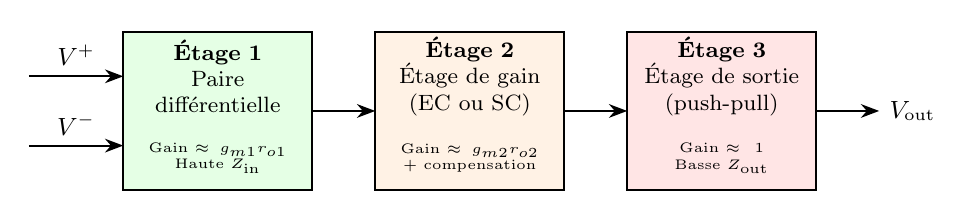
\begin{tikzpicture}[scale=0.8, >=Stealth, every node/.style={font=\small}]
  \draw[thick, fill=green!10] (0,0) rectangle (3,2.5);
  \node[font=\footnotesize, text width=2.5cm, align=center] at (1.5,1.8) {\textbf{Étage 1}\\Paire\\différentielle};
  \node[font=\tiny, text width=2.5cm, align=center] at (1.5,0.5) {Gain $\approx g_{m1} r_{o1}$\\Haute $Z_{\text{in}}$};
  \draw[thick, fill=orange!10] (4,0) rectangle (7,2.5);
  \node[font=\footnotesize, text width=2.5cm, align=center] at (5.5,1.8) {\textbf{Étage 2}\\Étage de gain\\(EC ou SC)};
  \node[font=\tiny, text width=2.5cm, align=center] at (5.5,0.5) {Gain $\approx g_{m2} r_{o2}$\\+ compensation};
  \draw[thick, fill=red!10] (8,0) rectangle (11,2.5);
  \node[font=\footnotesize, text width=2.5cm, align=center] at (9.5,1.8) {\textbf{Étage 3}\\Étage de sortie\\(push-pull)};
  \node[font=\tiny, text width=2.5cm, align=center] at (9.5,0.5) {Gain $\approx 1$\\Basse $Z_{\text{out}}$};
  \draw[->, thick] (-1.5,1.8) -- (0,1.8) node[midway, above]{$V^+$};
  \draw[->, thick] (-1.5,0.7) -- (0,0.7) node[midway, above]{$V^-$};
  \draw[->, thick] (3,1.25) -- (4,1.25);
  \draw[->, thick] (7,1.25) -- (8,1.25);
  \draw[->, thick] (11,1.25) -- (12,1.25) node[right]{$V_{\text{out}}$};
\end{tikzpicture}
\end{center}

\begin{formule}
\textbf{Gain en boucle ouverte :}
\[
\boxed{A_{OL} \approx (g_{m1} \cdot r_{o1}) \times (g_{m2} \cdot r_{o2}) \times A_3}
\]
Ce sont les $g_m$ et $r_o$ des chapitres 16 et 17 qui fixent le gain. Si $g_{m1} r_{o1} \approx 200$ et $g_{m2} r_{o2} \approx 500$ : $A_{OL} \approx 100\,000$ ($\SI{100}{dB}$).
\end{formule}

\begin{intuition}
\textbf{BJT vs MOSFET en entrée d'AOP :}
\begin{itemize}[nosep]
\item \textbf{Entrée BJT} (741, OP07, AD797) : $g_m$ élevé à faible courant $\Rightarrow$ gain élevé et bruit faible. Mais $I_B \neq 0$ ($\SI{10}{nA}$ à $\SI{1}{\micro A}$).
\item \textbf{Entrée JFET} (TL071, OPA134) : $I_B$ très faible ($\sim\SI{1}{pA}$--$\SI{50}{pA}$), bon compromis bruit/impédance.
\item \textbf{Entrée CMOS} (OPA340, LMC6482) : $I_B < \SI{1}{pA}$, alimentation basse tension, mais bruit $1/f$ plus élevé.
\end{itemize}
Le choix de la technologie d'entrée est le \textbf{premier critère} de sélection d'un AOP.
\end{intuition}

\subsection{La rétroaction négative : pourquoi et comment}

\begin{formule}
\textbf{Gain en boucle fermée :}
\[
\boxed{A_{CL} = \frac{A_{OL}}{1 + A_{OL}\,\beta} \approx \frac{1}{\beta}} \qquad \text{si } T = A_{OL}\,\beta \gg 1
\]
$\beta$ : fraction de retour. $T = A_{OL}\beta$ : gain de boucle.
\end{formule}

\begin{intuition}
\textbf{5 effets physiques de la rétroaction :}
\begin{enumerate}[nosep]
\item \textbf{Réduit le gain} de $A_{OL}$ (instable) à $1/\beta$ (précis, stable).
\item \textbf{Linéarise} : les non-linéarités sont divisées par $(1+T)$.
\item \textbf{Stabilise} : les variations de $A_{OL}$ (température, vieillissement) sont divisées par $(1+T)$.
\item \textbf{Réduit l'impédance de sortie} : $Z_{\text{out,BF}} = Z_{\text{out,BO}}/(1+T)$.
\item \textbf{Étend la bande passante} : le gain diminue mais la BP augmente, à produit constant (GBW).
\end{enumerate}
Le prix : risque d'\textbf{instabilité} si le déphasage dépasse $180°$ quand $|T| = 1$ (voir niveau ingénieur).
\end{intuition}

\subsection{Produit gain-bande et pôle dominant}

$A_{OL}$ diminue avec la fréquence. La plupart des AOP sont \textbf{compensés en interne} (un seul pôle dominant) :

\begin{formule}
\[
A_{OL}(f) = \frac{A_{OL,DC}}{1 + jf/f_p}
\]

Le \textbf{produit gain-bande} est constant :
\[
\boxed{GBW = A_{OL,DC} \times f_p = A_{CL} \times f_{-3\text{dB}}}
\]
Exemple (741) : $GBW = \SI{1}{MHz}$. En suiveur ($A_{CL} = 1$) : BP $= \SI{1}{MHz}$. En $\times 100$ : BP $= \SI{10}{kHz}$.
\end{formule}

\subsection{La compensation de Miller : le lien avec les transistors}

\begin{attention}
\textbf{C'est ici que les chapitres 16 et 17 deviennent essentiels.}

Sans compensation, les deux étages de gain (paire diff. + EC/SC) ont chacun un pôle. Deux pôles proches créent une pente de $-\SI{40}{dB/déc}$ avec $-180°$ de phase $\Rightarrow$ \textbf{oscillation} en boucle fermée.

\textbf{Solution : la compensation de Miller.} Un condensateur $C_C$ ($\sim\SI{20}{pF}$--$\SI{30}{pF}$) entre la sortie et l'entrée de l'étage 2. Par l'effet Miller ($C_{\text{Miller}} = C(1+|A_v|)$, chapitre 16) :
\begin{itemize}[nosep]
\item Le \textbf{premier pôle} descend vers les BF (capacité apparente $\times |A_{v2}|$).
\item Le \textbf{deuxième pôle} remonte vers les HF (``pole splitting'').
\end{itemize}
Résultat : un seul pôle dans la bande utile $\Rightarrow$ $-\SI{20}{dB/déc}$ $\Rightarrow$ stable ($M_\varphi \approx 60°$--$90°$).
\end{attention}

\begin{formule}
Pôles après compensation :
\[
f_{p1} \approx \frac{1}{2\pi\,g_{m2}\,r_{o1}\,r_{o2}\,C_C} \qquad f_{p2} \approx \frac{g_{m2}}{2\pi\,C_L}
\]
\end{formule}

\subsection{Le slew rate : une limitation en courant, pas en fréquence}

\begin{attention}
\textbf{Erreur classique :} le slew rate est souvent confondu avec une limitation de bande passante. C'est \textbf{faux}. C'est une limitation en \textbf{courant}.
\end{attention}

\begin{formule}
La paire différentielle d'entrée est polarisée par un courant de queue $I_{\text{tail}}$. Quand le signal d'entrée est grand ($V_d \gg V_T$), un des transistors prend tout le courant. Ce courant maximal charge le condensateur de compensation $C_C$ :
\[
\boxed{SR = \frac{I_{\text{tail}}}{C_C}}
\]
Le slew rate ne dépend \textbf{pas} de la fréquence, mais de l'\textbf{amplitude} du signal. Un sinusoïdal de fréquence $f$ et d'amplitude crête $V_p$ nécessite $SR_{\min} = 2\pi f V_p$.
\end{formule}

\subsection{Imperfections de l'AOP réel}

\begin{formule}
\begin{itemize}[nosep]
\item \textbf{Tension d'offset} ($V_{OS}$) : \SI{0.5}{mV}--\SI{5}{mV} (BJT), \SI{1}{mV}--\SI{10}{mV} (CMOS), $< \SI{25}{\micro V}$ (précision/chopper).
\item \textbf{Courant de polarisation} ($I_B$) : courant dans les entrées. BJT : \SI{10}{nA}--\SI{1}{\micro A}. CMOS : $< \SI{1}{pA}$.
\item \textbf{CMRR} : réjection du mode commun. $\SI{80}{dB}$--$\SI{120}{dB}$ en DC.
\item \textbf{PSRR} : réjection des variations d'alimentation.
\end{itemize}
\end{formule}

% ============================================================================
\section{Niveau Ingénieur}

\begin{ingenieur}
Stabilité, modèle fréquentiel complet, bruit, effets thermiques, saturation et recovery, et critères de choix pour la conception réelle.
\end{ingenieur}

\subsection{Stabilité : marges de phase et de gain}

\begin{formule}
\textbf{Condition de stabilité :} le gain de boucle $T(f)$ doit traverser $\SI{0}{dB}$ avec une pente de $-\SI{20}{dB/déc}$.

\[
\boxed{M_\varphi > 45° \quad \text{(minimum)}, \quad 60°\text{--}70° \quad \text{(recommandé)}}
\]

\textbf{Charge capacitive :} une $C_L$ en sortie crée un pôle $f_L = 1/(2\pi R_{\text{out}} C_L)$ qui réduit $M_\varphi$. Solutions : résistance d'isolation ($\sim\SI{50}{\ohm}$), ou AOP ``capacitive load stable''.
\end{formule}

\subsection{Modèle fréquentiel : pôles et zéros}

\begin{formule}
\[
A_{OL}(s) = \frac{A_{OL,DC}}{(1+s/\omega_{p1})(1+s/\omega_{p2})}
\]
Avec compensation : $f_{p1} \ll f_{p2}$. Le $\SI{0}{dB}$ est atteint à $f_T = GBW$ avec $\sim -90°$ $\Rightarrow$ marge $\approx 90°$ en théorie, $\sim 60°$--$70°$ en pratique.
\end{formule}

\begin{pratique}
\textbf{Bode typique (741) :} DC : \SI{100}{dB}. $f_{p1} \approx \SI{10}{Hz}$. $GBW \approx \SI{1}{MHz}$. $f_{p2} \approx \SI{3}{MHz}$. Phase à $f_T$ : $\approx -110°$ $\Rightarrow$ marge $\approx 70°$.
\end{pratique}

\subsection{Bruit de l'AOP}

\begin{formule}
Bruit total ramené à l'entrée :
\[
\boxed{e_{n,\text{total}} = \sqrt{e_n^2 + (i_n R_s)^2 + 4kTR_s}}
\]
\begin{itemize}[nosep]
\item $e_n$ : bruit en tension ($\text{nV}/\sqrt{\text{Hz}}$). Dominé par les transistors d'entrée.
\item $i_n$ : bruit en courant ($\text{pA}/\sqrt{\text{Hz}}$). Shot noise de $I_B$ (BJT), négligeable (CMOS).
\end{itemize}
\end{formule}

\begin{pratique}
\begin{center}
\renewcommand{\arraystretch}{1.4}
\begin{tabular}{p{2.5cm}p{2.5cm}p{2cm}p{5cm}}
\toprule
\textbf{Application} & \textbf{$R_s$ typique} & \textbf{Entrée} & \textbf{Justification} \\
\midrule
Audio (micro) & $< \SI{1}{k\ohm}$ & BJT & $e_n$ minimal ($\SI{1}{nV/\sqrt{Hz}}$) \\
Capteur piezo & $> \SI{10}{M\ohm}$ & JFET/CMOS & $i_n$ minimal \\
Instrumentation DC & $\SI{100}{\ohm}$--$\SI{10}{k\ohm}$ & BJT chopper & Offset $< \SI{1}{\micro V}$ \\
Transimpédance & $> \SI{1}{M\ohm}$ & JFET & $i_n$ faible \\
\bottomrule
\end{tabular}
\end{center}
\end{pratique}

\subsection{Effets thermiques}

\begin{formule}
\begin{itemize}[nosep]
\item \textbf{Offset} : dérive \SI{1}{\micro V/°C} (BJT) à \SI{10}{\micro V/°C} (CMOS). Chopper : $< \SI{0.05}{\micro V/°C}$.
\item \textbf{$I_B$ (BJT)} : double tous les \SI{10}{°C}.
\item \textbf{$g_m$} : diminue avec $T$ (MOSFET, $\mu \downarrow$), augmente (BJT, $V_T \downarrow$). $A_{OL}$ varie, mais la rétroaction absorbe ($\div(1+T)$).
\item \textbf{GBW} : varie de $\pm 20\%$ sur la plage de température.
\end{itemize}
\end{formule}

\subsection{Saturation et limites de sortie}

\begin{formule}
\begin{itemize}[nosep]
\item \textbf{Saturation en tension :} $V_{\text{out}} < V_{CC} - V_{\text{headroom}}$. Headroom : \SI{0.5}{V}--\SI{2}{V} (classique), $< \SI{50}{mV}$ (rail-to-rail output).
\item \textbf{Recovery time :} quand l'AOP sort de saturation, les transistors internes évacuent les charges stockées. Délai de \SI{1}{\micro s} à \SI{100}{\micro s}.
\item \textbf{Rail-to-rail input :} deux paires diff. (NMOS + PMOS) qui commutent $\Rightarrow$ discontinuité de $g_m$ et d'offset au croisement.
\end{itemize}
\end{formule}

% ========= RÉFLEXES INGÉNIEUR =========
\subsection{Réflexes à avoir avec un AOP}

\begin{pratique}
\textbf{Avant de commencer un design :}
\begin{enumerate}[nosep]
\item \textbf{Toujours vérifier les rails.} $V_{\text{out}}$ peut-il physiquement atteindre la valeur calculée ?
\item \textbf{Comparer la fréquence de travail au GBW.} Si $f > GBW/A_{CL}$ : le gain n'est plus garanti.
\item \textbf{Vérifier le slew rate pour les grands signaux.} $SR > 2\pi f V_p$ ? Sinon : distorsion.
\item \textbf{Attention aux sources haute impédance.} $I_B \times R_s$ crée un offset. Choisir BJT ($R_s$ faible), JFET/CMOS ($R_s$ élevé).
\item \textbf{Ne jamais supposer un AOP idéal} pour un design réel. Lire la datasheet.
\item \textbf{Charge capacitive :} ajouter une résistance d'isolation si $C_L > \SI{100}{pF}$.
\item \textbf{Découplage d'alimentation :} un condensateur de $\SI{100}{nF}$ au plus près de chaque broche $V_{CC}$/$V_{EE}$.
\end{enumerate}
\end{pratique}

% ========= CHECKLIST DEBUG =========
\subsection{Mon montage ne fonctionne pas --- que vérifier ?}

\begin{attention}
\textbf{Checklist de debug --- dans cet ordre :}

\textbf{1. L'alimentation est-elle correcte ?}

$V_{CC}$ et $V_{EE}$ (ou GND) sont-ils connectés et à la bonne tension ? Un AOP sans alimentation ne fait rien. Vérifier au multimètre \textit{sur les broches du composant}, pas sur le schéma.

\textbf{2. Les entrées sont-elles inversées ?}

$V^+$ et $V^-$ sont physiquement adjacentes et faciles à confondre. Si le retour va sur $V^+$ au lieu de $V^-$ : rétroaction positive $\Rightarrow$ oscillation ou saturation immédiate.

\textbf{3. La sortie est-elle saturée ?}

Mesurer $V_{\text{out}}$ : si elle est bloquée contre un rail ($\approx V_{CC}$ ou $\approx V_{EE}$), quelque chose force l'AOP en saturation (entrée trop grande, rétroaction positive, offset excessif en forte amplification).

\textbf{4. Y a-t-il une oscillation ?}

Regarder $V_{\text{out}}$ à l'oscilloscope. Si la sortie oscille à haute fréquence ($> \SI{100}{kHz}$) : problème de stabilité. Causes : charge capacitive, câblage trop long, manque de découplage, ou AOP non ``unity-gain stable'' utilisé à faible gain.

\textbf{5. Le slew rate est-il suffisant ?}

Si le signal de sortie est ``arrondi'' ou ``triangulaire'' au lieu d'être fidèle à l'entrée : le SR est trop faible pour l'amplitude et la fréquence du signal.

\textbf{6. La bande passante est-elle suffisante ?}

Si le gain diminue à la fréquence de travail : vérifier que $f < GBW/A_{CL}$.
\end{attention}

% === EXERCICES ===
\section*{Exercices}
\addcontentsline{toc}{section}{Exercices}

\subsection*{Niveau débutant}

\textbf{Exercice 18.1 ---} Un AOP monté en non-inverseur a $R_1 = \SI{1}{k\ohm}$ et $R_2 = \SI{9}{k\ohm}$. Quel est le gain ? Si $A_{OL} = \SI{80}{dB}$, quelle est l'erreur de gain ?

\begin{pratique}
\textbf{Solution :} $A_{CL} = 1 + R_2/R_1 = 10$. $A_{OL} = 10^4$. Erreur $= A_{CL}/(A_{CL}+A_{OL}) = 10/10010 = 0{,}1\%$.
\end{pratique}

\textbf{Exercice 18.2 ---} Un AOP a $GBW = \SI{10}{MHz}$. Bande passante pour $A_{CL} = 1$, $10$, $100$, $1000$ ?

\begin{pratique}
\textbf{Solution :} $f_{BW} = GBW/A_{CL}$. $A_{CL} = 1$ : \SI{10}{MHz}. $10$ : \SI{1}{MHz}. $100$ : \SI{100}{kHz}. $1000$ : \SI{10}{kHz}.
\end{pratique}

\subsection*{Niveau intermédiaire}

\textbf{Exercice 18.3 ---} Un AOP ($SR = \SI{13}{V/\micro s}$, $GBW = \SI{3}{MHz}$) en suiveur amplifie un signal de \SI{10}{V} crête. Fréquence max avant distorsion par slew rate ? Comparez avec la limite GBW.

\begin{pratique}
\textbf{Solution :} $f_{\max,SR} = SR/(2\pi V_p) = 13\times10^6/(2\pi\times10) = \SI{207}{kHz}$.

Limite petit signal : $f_{BW} = \SI{3}{MHz}$.

Le slew rate limite à \SI{207}{kHz}, soit $15\times$ moins que le GBW. C'est la contrainte dominante pour les grands signaux. Pour $V_p = \SI{100}{mV}$ : $f_{\max,SR} = \SI{20.7}{MHz}$ (GBW domine).
\end{pratique}

\textbf{Exercice 18.4 ---} Inverseur ($R_1 = \SI{10}{k\ohm}$, $R_2 = \SI{100}{k\ohm}$), AOP à entrée BJT ($I_B = \SI{200}{nA}$, $I_{OS} = \SI{20}{nA}$). Erreur de sortie due à $I_B$ ? Solution ?

\begin{pratique}
\textbf{Solution :} $V_{\text{err}} = I_B \times R_2 = 200\times10^{-9}\times10^5 = \SI{20}{mV}$.

Compensation : $R_3 = R_1 \parallel R_2 \approx \SI{9.1}{k\ohm}$ sur $V^+$. Erreur résiduelle : $I_{OS} \times R_2 = \SI{2}{mV}$ (réduction $\times 10$).
\end{pratique}

\subsection*{Niveau ingénieur}

\textbf{Exercice 18.5 ---} AOP : $f_{p1} = \SI{10}{Hz}$, $f_{p2} = \SI{5}{MHz}$, $A_{OL,DC} = \SI{100}{dB}$, bouclé en suiveur. (a) GBW et fréquence de croisement. (b) Marge de phase. (c) Ajout de $C_L = \SI{100}{pF}$ avec $R_{\text{out}} = \SI{100}{\ohm}$ : stable ?

\begin{pratique}
\textbf{Solution :}

(a) $GBW = 10^5\times10 = \SI{1}{MHz}$. Croisement à \SI{1}{MHz}.

(b) $\varphi = -\arctan(10^6/10) - \arctan(10^6/5\times10^6) = -90° - 11{,}3° = -101{,}3°$. $M_\varphi = 78{,}7°$. Excellent.

(c) $f_{p3} = 1/(2\pi\times100\times100\times10^{-12}) = \SI{15.9}{MHz}$. Phase additionnelle : $-3{,}6°$. $M_\varphi = 75{,}1°$. OK.

Mais si $C_L = \SI{10}{nF}$ : $f_{p3} = \SI{159}{kHz}$, $\varphi_{p3} = -81°$ $\Rightarrow$ $M_\varphi < 0$ $\Rightarrow$ \textbf{instable}.
\end{pratique}

\textbf{Exercice 18.6 ---} Comparez le bruit : AOP BJT ($e_n = \SI{3}{nV/\sqrt{Hz}}$, $i_n = \SI{1}{pA/\sqrt{Hz}}$) vs CMOS ($e_n = \SI{15}{nV/\sqrt{Hz}}$, $i_n = \SI{0.01}{pA/\sqrt{Hz}}$), pour $R_s = \SI{100}{\ohm}$ et $R_s = \SI{10}{M\ohm}$.

\begin{pratique}
\textbf{Solution :}

$R_s = \SI{100}{\ohm}$ : BJT $\Rightarrow e_{\text{tot}} = \SI{3.3}{nV/\sqrt{Hz}}$. CMOS $\Rightarrow \SI{15.1}{nV/\sqrt{Hz}}$. \textbf{BJT gagne} ($\times 4{,}6$).

$R_s = \SI{10}{M\ohm}$ : $e_{R_s} = \SI{12.9}{\micro V/\sqrt{Hz}}$ domine. BJT : $i_n R_s = \SI{10}{\micro V/\sqrt{Hz}}$, $e_{\text{tot}} = \SI{16.3}{\micro V/\sqrt{Hz}}$. CMOS : $i_n R_s \approx 0$, $e_{\text{tot}} = \SI{12.9}{\micro V/\sqrt{Hz}}$. \textbf{CMOS gagne} (le bruit en courant du BJT pénalise).
\end{pratique}

\subsection*{Questions de compréhension}

\begin{enumerate}[nosep]
\item Pourquoi le slew rate est-il une limitation ``grand signal'' et pas ``petit signal'' ? Quelle grandeur physique le limite ?
\item Un AOP rail-to-rail input utilise deux paires différentielles. Pourquoi le $g_m$ total n'est-il pas constant ?
\item Expliquez le rôle du condensateur de compensation Miller dans la séparation des pôles.
\item Calculez l'incertitude totale d'offset d'un AOP CMOS ($V_{OS} = \SI{5}{mV}$, $\SI{5}{\micro V/°C}$) sur $-40°$C à $+85°$C. Comparez avec un chopper ($V_{OS} < \SI{10}{\micro V}$, $< \SI{0.05}{\micro V/°C}$).
\end{enumerate}

% === RÉSUMÉ ===
\section*{Résumé du chapitre}
\addcontentsline{toc}{section}{Résumé du chapitre}

\begin{bases}[title={\color{white} Résumé --- Les Bases}]
\begin{center}
\renewcommand{\arraystretch}{1.3}
\begin{tabular}{p{3.5cm}p{9.5cm}}
\toprule
Principe & Amplifie $V^+ - V^-$ avec $A_{OL}$ très élevé (mais fini) \\
Règles d'or & $V^+ \approx V^-$ et $I^{\pm} \approx 0$ (approximations valides si rétroaction négative et $A_{OL}$ suffisant) \\
Méthode & Vérifier FB $\to$ $V^+=V^-$ $\to$ KCL à $V^-$ $\to$ isoler $V_{\text{out}}$ $\to$ vérifier saturation \\
Gain en BF & $1+R_2/R_1$ (non-inv.), $-R_2/R_1$ (inv.) \\
\bottomrule
\end{tabular}
\end{center}
\end{bases}

\begin{approfondissement}[title={\color{white} Résumé --- Approfondissement}]
\begin{center}
\renewcommand{\arraystretch}{1.3}
\begin{tabular}{p{3.5cm}p{9.5cm}}
\toprule
$A_{OL}$ & $\approx (g_{m1}r_{o1})(g_{m2}r_{o2})$ --- dépend de la polarisation et de la techno \\
Rétroaction & $A_{CL} = A_{OL}/(1+A_{OL}\beta) \approx 1/\beta$ si $T \gg 1$ \\
GBW & $= A_{OL,DC} \times f_{p1} = A_{CL} \times f_{BW}$ (constant) \\
Compensation & Miller interne : sépare les pôles ($C_C \sim \SI{30}{pF}$) \\
Slew rate & $SR = I_{\text{tail}}/C_C$ : limitation en \textbf{courant}, pas en fréquence \\
\bottomrule
\end{tabular}
\end{center}
\end{approfondissement}

\begin{ingenieur}[title={\color{white} Résumé --- Niveau Ingénieur}]
\begin{center}
\renewcommand{\arraystretch}{1.3}
\begin{tabular}{p{3.5cm}p{9.5cm}}
\toprule
Stabilité & $M_\varphi > 45°$ ($60°$--$70°$ idéal). Charge $C_L$ crée un pôle \\
Bruit & $e_{n,\text{tot}} = \sqrt{e_n^2 + (i_n R_s)^2 + 4kTR_s}$. BJT : faible $e_n$. CMOS : faible $i_n$ \\
Température & Offset : \SI{1}{\micro V/°C} (BJT) à \SI{10}{\micro V/°C} (CMOS). Chopper : $< \SI{0.05}{\micro V/°C}$ \\
Saturation & $V_{\text{out}} < V_{CC} - V_{\text{headroom}}$. Recovery time à la sortie \\
\bottomrule
\end{tabular}
\end{center}
\end{ingenieur}

% ============================================================================
% CHAPITRE 19 : FILTRES ACTIFS — LIMITES, CONCEPTION ET RÉALITÉ
% ============================================================================
% ============================================================================
% CHAPITRE 19 : FILTRES ACTIFS — LIMITES, CONCEPTION ET RÉALITÉ
% Complément au chapitre 14 (topologies et calculs de base)
% Fichier autonome à intégrer dans Bible_Elec.tex
% ============================================================================

\chapter{Filtres actifs : limites, conception et réalité}

\begin{center}
\textit{Le chapitre 14 a posé les fondations : topologies Sallen-Key et MFB,\\
calculs de $f_0$ et $Q$, dimensionnement des composants.\\
Ce chapitre transforme cette connaissance en compétence de conception :\\
comment passer d'un cahier des charges à un filtre réel qui fonctionne,\\
en anticipant les limites physiques qui séparent la théorie du PCB.}
\end{center}

\vspace{0.5cm}

Un filtre actif bien calculé sur le papier peut ne pas fonctionner en pratique. L'AOP n'est pas idéal (chapitre 18), les condensateurs ne sont pas parfaits, le bruit s'accumule, et les tolérances décalent $f_0$ et $Q$. Ce chapitre fournit la méthodologie complète pour concevoir un filtre réel et anticiper tous ces pièges, en s'appuyant sur la physique des pôles et zéros, les limites de l'AOP (chapitres 16--18), et la résonance (chapitre 12).

% ============================================================================
\section{Les Bases --- rappel et vue d'ensemble}

\begin{bases}
Reconnexion au chapitre 14 et introduction de la démarche de conception. Prérequis : chapitres 12 (résonance), 13 (Bode, fonctions de transfert), 14 (topologies Sallen-Key, MFB), 18 (AOP réel).
\end{bases}

\subsection{Ce que le chapitre 14 a établi}

Le chapitre 14 a présenté les outils de base du filtrage actif :

\begin{itemize}[nosep]
\item Les \textbf{quatre types} de filtres : passe-bas, passe-haut, passe-bande, coupe-bande (réjecteur).
\item La \textbf{cellule du 2nd ordre} comme brique élémentaire : $H(s) = H_0\omega_0^2/(s^2 + (\omega_0/Q)s + \omega_0^2)$, paramétrée par $f_0$ et $Q$.
\item Les \textbf{topologies} Sallen-Key (suiveur ou non-inverseur) et MFB (inverseur), avec les formules de dimensionnement.
\item La construction d'un filtre d'ordre $n$ par \textbf{cascade} de cellules du 2nd ordre.
\end{itemize}

Ce chapitre part de là et répond aux questions que le chapitre 14 n'aborde pas : \textit{comment choisir le bon type de filtre ? comment dimensionner pour un cahier des charges réel ? que se passe-t-il quand l'AOP n'est plus idéal ? pourquoi certains composants font-ils échouer le design ?}

\subsection{La physique derrière les pôles et les zéros}

Les pôles et zéros d'une fonction de transfert ne sont pas des abstractions. Ils correspondent à des \textbf{mécanismes physiques de stockage et d'échange d'énergie} dans le circuit, directement reliés à la résonance du chapitre 12.

\begin{formule}
\textbf{Un pôle = un réservoir d'énergie qui ralentit la réponse.}

Un condensateur stocke de l'énergie $E = \frac{1}{2}CV^2$. Pour que la tension à ses bornes change, il faut du \textit{temps} : $\tau = RC$. Au-delà de la fréquence $f_p = 1/(2\pi\tau)$, le condensateur ne peut plus ``suivre'' le signal $\Rightarrow$ atténuation de $-\SI{20}{dB/déc}$ et déphasage de $-90°$ par pôle.

\textbf{Physiquement :} le courant qui charge le condensateur est limité par la résistance. Plus la fréquence est élevée, moins le condensateur a le temps de se charger $\Rightarrow$ la tension de sortie diminue.
\end{formule}

\begin{formule}
\textbf{Un zéro = un chemin qui compense ou court-circuite.}

Un zéro crée l'effet inverse d'un pôle : $+\SI{20}{dB/déc}$ et $+90°$. Physiquement :
\begin{itemize}[nosep]
\item \textbf{Zéro à l'origine} ($s=0$) : le condensateur \textit{bloque le DC} et laisse passer l'AC $\Rightarrow$ filtre passe-haut.
\item \textbf{Zéro à une fréquence finie} : un chemin alternatif (résonance série $LC$, branche de rétroaction) \textit{annule la transmission} à cette fréquence $\Rightarrow$ filtre coupe-bande (notch).
\item \textbf{Zéro qui compense un pôle} : dans un filtre passe-tout ou un compensateur (lead), un zéro ``annule'' l'atténuation d'un pôle, laissant passer le signal tout en modifiant la phase.
\end{itemize}
\end{formule}

\begin{intuition}
\textbf{Lien avec la résonance (chapitre 12) :} le filtre du 2nd ordre est exactement un circuit résonant. Le paramètre $Q$ a la même signification qu'en résonance RLC :
\[
Q = \frac{\text{énergie stockée par cycle}}{\text{énergie dissipée par cycle}} = \frac{f_0}{\Delta f_{-3\text{dB}}}
\]
\begin{itemize}[nosep]
\item $Q$ élevé $\Rightarrow$ beaucoup d'énergie stockée, peu dissipée $\Rightarrow$ résonance marquée (pic), temps de stabilisation long.
\item $Q$ faible $\Rightarrow$ énergie rapidement dissipée $\Rightarrow$ pas de résonance, réponse amortie.
\end{itemize}
Le filtre Butterworth ($Q = 0{,}707$) est au seuil critique : juste assez d'amortissement pour ne pas faire de pic.
\end{intuition}

% ============================================================================
\section{Approfondissement --- Méthodologie de conception}

\vspace{0.3cm}
\textit{Le chapitre 14 montre comment calculer un filtre. Cette section montre comment \textbf{concevoir} un filtre : partir d'un besoin réel et arriver à un schéma fonctionnel avec des valeurs de composants vérifiées.}
\vspace{0.3cm}

\begin{approfondissement}
Procédure complète de conception, choix du type de filtre, normalisation, mise à l'échelle, et lien temporel/fréquentiel. Prérequis : chapitre 14 (calculs de base), chapitre 13 (Bode).
\end{approfondissement}

\subsection{Étape 1 : le cahier des charges}

\begin{pratique}
Avant tout calcul, définir précisément :

\begin{enumerate}[nosep]
\item \textbf{Type de filtre} : passe-bas, passe-haut, passe-bande, coupe-bande ?
\item \textbf{Fréquence de coupure} $f_c$ (à $-\SI{3}{dB}$, ou à une autre valeur si spécifié).
\item \textbf{Atténuation requise} : par exemple ``$> \SI{60}{dB}$ à \SI{100}{kHz}'' $\Rightarrow$ détermine l'ordre.
\item \textbf{Ondulation maximale} en bande passante : $0$ (Butterworth/Bessel), ou $0{,}5$/$1$/$3$ dB (Tchebychev).
\item \textbf{Contraintes sur la phase} : la phase doit-elle être linéaire (signaux impulsionnels, données) ? $\Rightarrow$ Bessel.
\item \textbf{Contraintes système} : alimentation disponible, gamme de température, bruit maximal admissible, impédance source et charge.
\end{enumerate}
\end{pratique}

\subsection{Étape 2 : choix du type de filtre}

\begin{formule}
\textbf{Le compromis fondamental du filtrage :} on ne peut \textbf{pas} avoir simultanément une bande passante parfaitement plate, une transition infiniment raide, et une phase parfaitement linéaire. Chaque type de filtre sacrifie un aspect :

\begin{center}
\renewcommand{\arraystretch}{1.5}
\begin{tabular}{p{2.5cm}p{3cm}p{3cm}p{4.5cm}}
\toprule
\textbf{Type} & \textbf{Bande passante} & \textbf{Transition} & \textbf{Phase / temporel} \\
\midrule
\textbf{Butterworth} & Maximalement plate & Modérée & Dépassement faible ($4{,}3\%$ pour ordre 2) \\
\textbf{Tchebychev} & Ondulation ($\leq$ ripple) & \textbf{Plus raide} à même ordre & Dépassement élevé \\
\textbf{Bessel} & Douce (pas optimale) & La plus douce & \textbf{Phase linéaire}, pas de déformation \\
\textbf{Elliptique} (Cauer) & Ondulation BP + BC & \textbf{La plus raide} & Forte distorsion de phase \\
\bottomrule
\end{tabular}
\end{center}
\end{formule}

\begin{intuition}
\textbf{Règle de choix rapide :}
\begin{itemize}[nosep]
\item Pas de contrainte particulière $\Rightarrow$ \textbf{Butterworth} (le choix par défaut).
\item Signaux impulsionnels, données numériques, métrologie $\Rightarrow$ \textbf{Bessel} (phase linéaire, pas de ringing).
\item Spécification d'atténuation très sévère avec ordre minimal $\Rightarrow$ \textbf{Tchebychev} (si ondulation tolérée).
\item Rejet d'une fréquence précise avec ordre minimal $\Rightarrow$ \textbf{Elliptique}.
\end{itemize}
\end{intuition}

\subsection{Étape 3 : détermination de l'ordre}

L'ordre du filtre détermine la raideur de la transition entre bande passante et bande coupée.

\begin{formule}
\textbf{Pour un Butterworth :}
\[
|H(f_s)|^2 = \frac{1}{1+(f_s/f_c)^{2n}}
\]

L'atténuation à la fréquence $f_s$ est $A = 10\log_{10}(1+(f_s/f_c)^{2n})$ dB. On résout pour $n$ :
\[
\boxed{n \geq \frac{\log(10^{A/10} - 1)}{2\log(f_s/f_c)}}
\]
Arrondir à l'entier supérieur.
\end{formule}

\begin{pratique}
\textbf{Exemple :} $f_c = \SI{20}{kHz}$, atténuation $> \SI{60}{dB}$ à $f_s = \SI{100}{kHz}$.

$f_s/f_c = 5$. $n \geq \log(10^6-1)/(2\log5) = 6/1{,}398 = 4{,}29$. $\Rightarrow$ $n = 5$.
\end{pratique}

\subsection{Étape 4 : prototype normalisé et tables de $Q$}

On utilise des tables de \textbf{pôles normalisés} qui donnent les $Q_k$ et $f_{0,k}$ de chaque cellule du 2nd ordre. Le filtre prototype est normalisé à $\omega_0 = \SI{1}{rad/s}$.

\begin{formule}
\textbf{Tables Butterworth ($f_{0,k} = f_c$ pour toutes les cellules) :}

\begin{center}
\begin{tabular}{cll}
\toprule
\textbf{Ordre} & \textbf{$Q$ des cellules} & \textbf{Composition} \\
\midrule
2 & $0{,}7071$ & 1 cellule 2nd ordre \\
3 & $1{,}0000$ & 1 cellule 2nd ordre + 1 cellule 1er ordre \\
4 & $0{,}5412$ \quad $1{,}3066$ & 2 cellules 2nd ordre \\
5 & $0{,}6180$ \quad $1{,}6180$ & 2 cellules 2nd ordre + 1 cellule 1er ordre \\
6 & $0{,}5176$ \quad $0{,}7071$ \quad $1{,}9319$ & 3 cellules 2nd ordre \\
\bottomrule
\end{tabular}
\end{center}
\end{formule}

\begin{attention}
\textbf{Ordre de cascade :} la cellule de \textbf{plus haut $Q$} se place en \textbf{dernier}. Son pic de résonance amplifie le signal de $Q$ en linéaire ($20\log Q$ en dB). Si elle est en tête, le signal amplifié peut \textbf{saturer l'AOP} des étages suivants. En la plaçant en dernier, le signal a déjà été atténué par les cellules précédentes dans la zone du pic.
\end{attention}

\subsection{Étape 5 : mise à l'échelle fréquence/impédance}

Le prototype normalisé ($\omega_0 = 1$, $R = \SI{1}{\ohm}$) est inutilisable directement. On le redimensionne :

\begin{formule}
\textbf{Mise à l'échelle :}
\[
\boxed{R_{\text{réel}} = R_{\text{norm}} \times Z_0} \qquad \boxed{C_{\text{réel}} = \frac{C_{\text{norm}}}{\omega_c \times Z_0}}
\]
$Z_0$ : impédance de référence choisie (typiquement \SI{1}{k\ohm} à \SI{100}{k\ohm}).

$\omega_c = 2\pi f_c$ : pulsation de coupure cible.

\textbf{Choix de $Z_0$ :} compromis entre bruit ($Z_0$ faible $\Rightarrow$ bruit thermique faible mais courant AOP élevé) et valeurs de condensateurs réalistes ($Z_0$ trop faible $\Rightarrow$ condensateurs énormes).
\end{formule}

\subsection{Étape 6 : implémentation en cellules}

Pour chaque cellule du 2nd ordre, on utilise la topologie choisie (Sallen-Key ou MFB, chapitre 14) et on calcule les valeurs de composants à partir de $f_{0,k}$, $Q_k$ et $Z_0$.

\begin{formule}
\textbf{Sallen-Key passe-bas, composants égaux en résistance ($R_1 = R_2 = R$) :}
\[
C_1 = 2Q \cdot C_{\text{ref}} \qquad C_2 = \frac{C_{\text{ref}}}{2Q} \qquad \text{avec } C_{\text{ref}} = \frac{1}{2\pi R f_0}
\]
Vérification : $C_1 \times C_2 = C_{\text{ref}}^2$ et $\sqrt{C_1/C_2} = 2Q$.
\end{formule}

\begin{pratique}
Arrondir les valeurs aux séries normalisées E24 ($\pm 5\%$) ou E96 ($\pm 1\%$). Chaque arrondi décale légèrement $f_0$ et $Q$ : c'est inévitable, mais la simulation finale le vérifiera.
\end{pratique}

\subsection{Étape 7 : vérification}

\begin{pratique}
\textbf{Checklist de vérification (obligatoire avant fabrication) :}

\begin{enumerate}[nosep]
\item \textbf{Simulation Bode} (AC analysis) : le gabarit d'atténuation est-il respecté ? La fréquence de coupure est-elle correcte ?
\item \textbf{Réponse temporelle} (transitoire) : le dépassement est-il acceptable ? Le temps de stabilisation ?
\item \textbf{Modèle réel de l'AOP} : utiliser le modèle SPICE du fabricant, pas un AOP idéal. Vérifier que le gain de boucle est suffisant à $f_0$ et que la sortie ne sature pas.
\item \textbf{Analyse Monte Carlo} : faire varier les composants aléatoirement selon leurs tolérances ($\pm 1\%$ résistances, $\pm 5\%$ condensateurs C0G). Vérifier que le filtre respecte encore le gabarit dans $99\%$ des cas.
\item \textbf{Bruit} : simuler le bruit en sortie. Est-il compatible avec le rapport signal/bruit requis ?
\end{enumerate}
\end{pratique}

\subsection{Lien temporel $\leftrightarrow$ fréquentiel : le rôle de $Q$}

$Q$ détermine \textbf{simultanément} la réponse en fréquence et la réponse temporelle. C'est la même physique vue sous deux angles :

\begin{formule}
\textbf{Dépassement de la réponse indicielle} (2nd ordre) :
\[
\boxed{D\% = 100 \times e^{-\pi/\sqrt{4Q^2 - 1}}} \qquad (Q > 0{,}5)
\]

\begin{center}
\renewcommand{\arraystretch}{1.4}
\begin{tabular}{lccc}
\toprule
\textbf{Type} & \textbf{$Q$} & \textbf{Pic (dB)} & \textbf{Dépassement (\%)} \\
\midrule
Bessel (ordre 2) & $0{,}577$ & $0$ & $0{,}4$ \\
Butterworth & $0{,}707$ & $0$ & $4{,}3$ \\
Tchebychev $\SI{0.5}{dB}$ & $0{,}864$ & $0{,}5$ & $13$ \\
Tchebychev $\SI{1}{dB}$ & $0{,}957$ & $1$ & $21$ \\
Tchebychev $\SI{3}{dB}$ & $1{,}306$ & $3$ & $39$ \\
\bottomrule
\end{tabular}
\end{center}
\end{formule}

\begin{intuition}
\textbf{Pourquoi $Q$ élevé donne un dépassement :} un $Q$ élevé signifie que les condensateurs stockent \textit{beaucoup d'énergie} par rapport à ce que les résistances dissipent à chaque cycle. Quand un échelon arrive, l'énergie s'accumule dans les condensateurs et ne peut pas être dissipée assez vite $\Rightarrow$ le signal ``dépasse'' la valeur finale et oscille avant de se stabiliser. C'est exactement le même phénomène que la résonance du chapitre 12 : un circuit RLC à fort $Q$ ``sonne'' longtemps après une excitation.
\end{intuition}

% ============================================================================
\section{Niveau Ingénieur}

\begin{ingenieur}
Limites dues à l'AOP réel, sensibilité aux tolérances, bruit, et cas de conception complet. Lien avec les chapitres 16--18 (transistors et AOP).
\end{ingenieur}

\subsection{L'AOP réel dans le filtre : trois limites critiques}

Le chapitre 14 suppose un AOP idéal. Le chapitre 18 a montré que l'AOP a un gain fini qui diminue avec la fréquence ($A_{OL}(f) = GBW/f$), un slew rate limité ($SR = I_{\text{tail}}/C_C$, chapitre 18), et un déphasage qui s'accumule. Ces trois limitations modifient profondément le comportement du filtre.

\subsubsection*{1. GBW insuffisant $\Rightarrow$ $Q$ effectif qui dérive}

\begin{formule}
Le filtre repose sur le \textbf{gain de boucle} de l'AOP pour maintenir $f_0$ et $Q$ à leurs valeurs nominales. Quand la fréquence augmente et que $A_{OL}$ diminue, le gain de boucle n'est plus suffisant :
\begin{itemize}[nosep]
\item $f_0$ effective se \textbf{décale} vers le bas.
\item $Q$ effectif \textbf{augmente} (le filtre résonne plus fort que prévu).
\item Si $Q_{\text{eff}} \to \infty$ : \textbf{oscillation}.
\end{itemize}

\textbf{Règle de conception} (valable pour Sallen-Key et MFB) :
\[
\boxed{GBW_{\text{AOP}} > 10 \cdot Q \cdot f_0}
\]
Le facteur $10$ garantit une erreur $< 1\%$ sur $f_0$ et $Q$. Pour des applications de précision, utiliser un facteur $100$.
\end{formule}

\begin{pratique}
\textbf{Exemple :} filtre Butterworth ordre 6 à $f_c = \SI{48}{kHz}$. La cellule de plus haut $Q$ a $Q_3 = 1{,}932$.

$GBW_{\min} = 10\times1{,}932\times48000 = \SI{928}{kHz}$.

Un TL072 ($GBW = \SI{3}{MHz}$) convient ($\times 3{,}2$ de marge). Un LM358 ($GBW = \SI{1}{MHz}$) est marginal. Un 741 ($GBW = \SI{1}{MHz}$) est juste acceptable mais sans marge --- à éviter.
\end{pratique}

\subsubsection*{2. Slew rate $\Rightarrow$ distorsion grand signal}

\begin{attention}
Le slew rate de l'AOP (chapitre 18 : $SR = I_{\text{tail}}/C_C$) est une limitation en \textbf{courant}, pas en fréquence. Mais un filtre à $Q$ élevé \textbf{amplifie} le signal au voisinage de $f_0$ d'un facteur $Q$ (en linéaire). La sortie de l'AOP doit donc fournir un signal plus grand que l'entrée :

\[
\boxed{SR > 2\pi f_0 \cdot Q \cdot V_{\text{in,crête}}}
\]

\textbf{Le piège :} un signal d'entrée de $\SI{1}{V}$ crête dans un filtre à $Q = 10$ peut produire $\SI{10}{V}$ crête en sortie au voisinage de $f_0$. Si l'AOP a $SR = \SI{2}{V/\micro s}$ et $f_0 = \SI{100}{kHz}$ : $SR_{\min} = 2\pi\times10^5\times10\times1 = \SI{6.28}{V/\micro s}$ $\Rightarrow$ \textbf{distorsion}.
\end{attention}

\begin{intuition}
\textbf{D'où vient physiquement le slew rate (lien avec les chapitres 16--18) :}

Le slew rate n'est pas une limite abstraite. Il correspond à la capacité maximale des transistors de l'étage d'entrée (paire différentielle) à fournir le courant nécessaire pour charger le \textbf{condensateur de compensation interne $C_C$} --- le condensateur de Miller qui crée le pôle dominant de l'AOP (chapitre 18).

Quand la tension différentielle d'entrée $V_d$ dépasse quelques $V_T$ ($\approx \SI{26}{mV}$, chapitre 16), un des transistors de la paire prend \textit{tout} le courant de queue $I_{\text{tail}}$ et l'autre se bloque. Le courant maximal disponible pour charger $C_C$ est donc $I_{\text{tail}}$, d'où :
\[
SR = \frac{I_{\text{tail}}}{C_C} = \frac{dV_{\text{out}}}{dt}\bigg|_{\max}
\]

On retrouve ici la chaîne causale complète \textbf{transistor $\to$ AOP $\to$ filtre} : le $g_m$ et le courant de polarisation de la paire différentielle (fixés par la physique du BJT ou du MOSFET, chapitres 16--17) déterminent $I_{\text{tail}}$, qui détermine le SR de l'AOP, qui limite la pente maximale du signal dans le filtre.
\end{intuition}

\subsubsection*{3. Déphasage de l'AOP $\Rightarrow$ problème de stabilité}

L'AOP n'est pas un simple gain à la fréquence $f_0$ : il introduit un \textbf{déphasage} ($-90°$ au pôle dominant, plus au-delà). Ce déphasage s'ajoute à celui du filtre lui-même. Pour un filtre à fort $Q$, la boucle de rétroaction est ``tendue'' et le déphasage supplémentaire de l'AOP peut faire basculer le circuit dans l'\textbf{instabilité} (oscillation).

\begin{formule}
\textbf{Vérification :} simuler le gain de boucle $T(s)$ du circuit complet (filtre + AOP) et vérifier que la marge de phase est $> 45°$ à la fréquence où $|T| = 1$. Si la marge est insuffisante : choisir un AOP plus rapide, réduire $Q$, ou passer à une topologie moins sensible (state-variable, biquad).
\end{formule}

\begin{intuition}
\textbf{Vision ``système'' : le filtre comme boucle fermée.}

Un filtre actif est un système en \textbf{boucle fermée}. Son comportement est gouverné par le gain de boucle $T(s) = A_{OL}(s)\cdot\beta(s)$, et ses pôles réels sont les racines de l'équation caractéristique $1 + T(s) = 0$.

Quand le gain de l'AOP diminue en haute fréquence (au-delà de $f_p = GBW/A_{OL,DC}$, chapitre 18), le gain de boucle $T(s)$ s'effondre. Cela \textbf{déplace les pôles} du filtre par rapport à leur position théorique (calculée avec un AOP idéal). Concrètement :
\begin{itemize}[nosep]
\item Les pôles se rapprochent de l'axe imaginaire $\Rightarrow$ $Q_{\text{eff}} > Q_{\text{nominal}}$.
\item Si les pôles atteignent l'axe imaginaire $\Rightarrow$ $Q = \infty$ $\Rightarrow$ \textbf{oscillation}.
\end{itemize}

La condition $GBW \gg Q \cdot f_0$ garantit que le gain de boucle reste suffisamment élevé pour ``maintenir'' les pôles à l'emplacement prévu par les calculs idéaux. C'est exactement le même raisonnement que la stabilité en rétroaction du chapitre 18, appliqué au filtre.
\end{intuition}

\subsection{Sensibilité aux tolérances des composants}

\begin{formule}
La \textbf{sensibilité} mesure comment une variation relative d'un composant $x$ affecte un paramètre $P$ du filtre :
\[
S_x^P = \frac{x}{P}\frac{\partial P}{\partial x}
\]

\textbf{Résultats typiques pour un Sallen-Key :}
\begin{itemize}[nosep]
\item $S_R^{f_0} = -1/2$ et $S_C^{f_0} = -1/2$ : une variation de $+1\%$ sur $R$ ou $C$ décale $f_0$ de $-0{,}5\%$. Modéré.
\item $S_C^Q$ dépend fortement de $Q$. Pour $Q > 10$, la sensibilité de $Q$ aux composants devient \textbf{très élevée} : une variation de $1\%$ sur un condensateur peut changer $Q$ de $10\%$ ou plus.
\end{itemize}
\end{formule}

\begin{attention}
\textbf{Conséquence pratique :}
\begin{itemize}[nosep]
\item Pour $Q < 3$ : Sallen-Key ou MFB avec composants E96 ($\pm 1\%$) et condensateurs C0G/NP0 ($\pm 5\%$, stables). Aucun problème.
\item Pour $3 < Q < 10$ : MFB préféré (moindre sensibilité). Résistances $\pm 0{,}1\%$ si possible. Condensateurs C0G obligatoires.
\item Pour $Q > 10$ : les topologies Sallen-Key et MFB deviennent impraticables. Passer à une topologie \textbf{state-variable} ou \textbf{biquad} dont la sensibilité de $Q$ est intrinsèquement faible (chaque paramètre est fixé par un seul composant).
\end{itemize}
\end{attention}

\begin{pratique}
\textbf{Choix des condensateurs :}
\begin{center}
\renewcommand{\arraystretch}{1.3}
\begin{tabular}{p{2.5cm}p{2cm}p{2.5cm}p{5.5cm}}
\toprule
\textbf{Type} & \textbf{Tolérance} & \textbf{Stabilité} & \textbf{Usage filtrage} \\
\midrule
\textbf{C0G/NP0} & $\pm 5\%$ & Excellente & \textbf{Obligatoire} pour filtres de précision \\
X7R & $\pm 10\%$ & Médiocre & Découplage uniquement. $C$ varie $\pm 15\%$ en $T$ et $-30\%$ avec la tension DC \\
X5R & $\pm 20\%$ & Mauvaise & \textbf{Interdit} en filtrage \\
Film PP & $\pm 1\%$--$5\%$ & Très bonne & Excellent mais encombrant \\
\bottomrule
\end{tabular}
\end{center}

Un condensateur X7R de \SI{100}{nF}/\SI{16}{V} peut valoir \SI{70}{nF} avec \SI{10}{V} DC appliqués. Si utilisé dans un filtre, $f_0$ serait décalé de $+20\%$. C'est un piège extrêmement courant.
\end{pratique}

\subsection{Bruit dans les filtres actifs}

\begin{formule}
Le bruit en sortie d'un filtre actif a trois origines :

\textbf{1. Bruit thermique des résistances :}
$\overline{v^2} = 4kTR\Delta f$ pour chaque résistance. Plus $R$ est élevé, plus le bruit est élevé.

\textbf{2. Bruit de l'AOP :}
\begin{itemize}[nosep]
\item Le bruit en tension $e_n$ de l'AOP est \textbf{amplifié} par le gain du filtre dans la bande passante, puis atténué en bande coupée.
\item Le bruit en courant $i_n$ est converti en tension par les résistances du filtre.
\end{itemize}

\textbf{3. Accumulation en cascade :}
Chaque cellule ajoute son propre bruit. Le bruit des \textbf{premières cellules} est le plus critique car il est amplifié par les cellules suivantes.

\textbf{Règles de conception pour minimiser le bruit :}
\begin{itemize}[nosep]
\item Résistances $< \SI{100}{k\ohm}$ (compromis bruit/courant AOP).
\item Cellule de plus faible $Q$ en \textbf{premier} (gain le plus plat $\Rightarrow$ n'amplifie pas le bruit).
\item AOP à faible $e_n$ si le signal filtré est faible.
\item Ne pas surdimensionner l'ordre : chaque cellule ajoutée ajoute du bruit.
\end{itemize}
\end{formule}

\subsection{Cas de conception complet : anti-aliasing pour ADC audio}

\begin{pratique}
\textbf{Cahier des charges :}
\begin{itemize}[nosep]
\item ADC audio 24 bits, $f_s = \SI{48}{kHz}$.
\item Signal utile : $\SI{20}{Hz}$ à $\SI{20}{kHz}$.
\item Filtre anti-aliasing passe-bas : $f_c = \SI{20}{kHz}$.
\item Atténuation $> \SI{60}{dB}$ à $f_s/2 = \SI{24}{kHz}$ : \textbf{irréaliste en analogique} ($24/20 = 1{,}2$ seulement). Solution : l'ADC utilise un suréchantillonnage interne ($f_s = \SI{6.144}{MHz}$). Le filtre anti-aliasing doit atténuer $> \SI{60}{dB}$ à $f_s/2 = \SI{3.072}{MHz}$.
\item $f_s/f_c = 3072/20 = 153{,}6$ ($\sim 2{,}2$ décades).
\item Ondulation en bande passante : $< \SI{0.1}{dB}$ (audio haute fidélité $\Rightarrow$ Butterworth).
\item Bruit : compatible avec 24 bits ($\sim \SI{120}{dB}$ de dynamique $\Rightarrow$ $V_{\text{bruit}} < \SI{10}{\micro V_{rms}}$ sur la bande audio).
\end{itemize}
\end{pratique}

\begin{pratique}
\textbf{Dimensionnement :}

\textbf{Ordre :} $n \geq \log(10^6)/(2\log153{,}6) = 6/4{,}37 = 1{,}37$. $\Rightarrow$ $n = 2$ suffit ! (grâce au suréchantillonnage, le ratio $f_s/f_c$ est très favorable).

Un \textbf{Butterworth d'ordre 2} ($Q = 0{,}707$) donne $\SI{-80}{dB}$ à \SI{3}{MHz} ($= 150\times f_c$, soit $40\log150 = \SI{87}{dB}$). Largement suffisant.

\textbf{Topologie :} Sallen-Key gain unitaire (simple, $Q = 0{,}707$ modéré).

\textbf{Composants :} $R = \SI{3.3}{k\ohm}$ (E24).

$C_{\text{ref}} = 1/(2\pi\times3300\times20000) = \SI{2.41}{nF}$.

$C_1 = 2\times0{,}707\times2{,}41 = \SI{3.41}{nF} \to \SI{3.3}{nF}$ (E24, C0G).

$C_2 = 2{,}41/(2\times0{,}707) = \SI{1.70}{nF} \to \SI{1.8}{nF}$ (E24, C0G).

$f_0$ réelle $= 1/(2\pi\times3300\times\sqrt{3{,}3\times1{,}8}\times10^{-9}) = \SI{19.8}{kHz}$. Erreur : $-1\%$. Acceptable.

\textbf{AOP :} $GBW > 10\times0{,}707\times20000 = \SI{141}{kHz}$. N'importe quel AOP audio convient (NE5532 : $GBW = \SI{10}{MHz}$, $e_n = \SI{5}{nV/\sqrt{Hz}}$, $SR = \SI{9}{V/\micro s}$).

$SR$ : $V_{\text{in,max}} = \SI{2}{V_{rms}} \approx \SI{2.83}{V_{crête}}$. $SR_{\min} = 2\pi\times20000\times0{,}707\times2{,}83 = \SI{0.25}{V/\micro s}$. NE5532 : $SR = \SI{9}{V/\micro s}$ $\Rightarrow$ marge de $\times 36$. OK.

\textbf{Bruit :} $e_n = \SI{5}{nV/\sqrt{Hz}}$. Bruit dans la bande audio ($\SI{20}{kHz}$) : $5\times\sqrt{20000} = \SI{0.71}{\micro V_{rms}}$. Bruit de $R$ : $\sqrt{4kT\times3300\times20000} = \SI{1.04}{\micro V_{rms}}$. Bruit total : $\sqrt{0{,}71^2+1{,}04^2} = \SI{1.26}{\micro V_{rms}}$. Bien en dessous du seuil de $\SI{10}{\micro V_{rms}}$.
\end{pratique}

\begin{attention}
\textbf{Les erreurs à ne pas commettre dans cet exemple :}
\begin{enumerate}[nosep]
\item \textbf{Calculer l'ordre sans le suréchantillonnage} : sans suréchantillonnage ($f_s = \SI{48}{kHz}$, Nyquist à $\SI{24}{kHz}$), il faudrait $\SI{60}{dB}$ en seulement $1{,}2\times f_c$ $\Rightarrow$ ordre $> 25$ en analogique. Totalement irréaliste. Le suréchantillonnage est \textbf{indispensable}.
\item \textbf{Utiliser des condensateurs X7R} : un X7R de \SI{3.3}{nF} sous \SI{3}{V} DC peut valoir \SI{2.5}{nF} $\Rightarrow$ $f_c$ décalé de $+15\%$.
\item \textbf{Oublier le bruit du circuit} : avec un AOP bruyant ($e_n = \SI{30}{nV/\sqrt{Hz}}$), le bruit serait $\SI{4.2}{\micro V_{rms}}$ --- toujours acceptable ici, mais critique pour un ADC 32 bits.
\item \textbf{Négliger le layout} : un filtre anti-aliasing mal routé (boucle de masse, couplage capacitif) peut injecter du bruit HF directement dans l'ADC, annulant le bénéfice du filtre.
\end{enumerate}
\end{attention}

% === EXERCICES ===
\section*{Exercices}
\addcontentsline{toc}{section}{Exercices}

\subsection*{Niveau débutant}

\textbf{Exercice 19.1 ---} Quel type de filtre (Butterworth, Bessel, Tchebychev) choisiriez-vous pour : (a) un filtre anti-aliasing ADC, (b) un récepteur de données NRZ à \SI{1}{Mbit/s}, (c) un filtre audio avec réjection maximale du \SI{50}{Hz} secteur ?

\begin{pratique}
\textbf{Solution :}

(a) \textbf{Butterworth} : bande passante plate (pas d'ondulation), transition raisonnablement raide.

(b) \textbf{Bessel} : phase linéaire indispensable pour ne pas déformer les fronts des impulsions NRZ. Un Butterworth créerait du ringing ($4{,}3\%$ de dépassement par cellule).

(c) Pour rejeter le \SI{50}{Hz} : un filtre \textbf{coupe-bande} (notch) centré sur \SI{50}{Hz}, pas un passe-bas. Topologie twin-T ou Wien. Si on veut un passe-haut pour couper tout en dessous de \SI{100}{Hz} : Butterworth suffit.
\end{pratique}

\textbf{Exercice 19.2 ---} Calculez l'ordre d'un filtre Butterworth avec $f_c = \SI{1}{kHz}$ et $\SI{40}{dB}$ d'atténuation à \SI{5}{kHz}.

\begin{pratique}
\textbf{Solution :} $f_s/f_c = 5$. $n \geq \log(10^4-1)/(2\log5) = 4/(2\times0{,}699) = 2{,}86$. $\Rightarrow$ $n = 3$.
\end{pratique}

\subsection*{Niveau intermédiaire}

\textbf{Exercice 19.3 ---} Dimensionnez un filtre Butterworth passe-bas d'ordre 4 à $f_c = \SI{10}{kHz}$ en Sallen-Key, $R = \SI{10}{k\ohm}$. Donnez les valeurs de $C_1$, $C_2$ pour chaque cellule.

\begin{pratique}
\textbf{Solution :} $Q_1 = 0{,}541$, $Q_2 = 1{,}307$. $C_{\text{ref}} = 1/(2\pi\times10^4\times10^4) = \SI{1.59}{nF}$.

Cellule 1 : $C_1 = 2\times0{,}541\times1{,}59 = \SI{1.72}{nF} \to \SI{1.8}{nF}$. $C_2 = 1{,}59/(2\times0{,}541) = \SI{1.47}{nF} \to \SI{1.5}{nF}$.

Cellule 2 : $C_1 = 2\times1{,}307\times1{,}59 = \SI{4.16}{nF} \to \SI{3.9}{nF}$. $C_2 = 1{,}59/(2\times1{,}307) = \SI{0.608}{nF} \to \SI{680}{pF}$.

Cellule 2 en dernier (haut $Q$).
\end{pratique}

\textbf{Exercice 19.4 ---} L'exercice 19.3 utilise un AOP avec $GBW = \SI{500}{kHz}$. Est-ce suffisant pour la cellule de plus haut $Q$ ? Que se passe-t-il si on utilise un AOP avec $GBW = \SI{100}{kHz}$ ?

\begin{pratique}
\textbf{Solution :} $GBW_{\min} = 10\times Q_2\times f_c = 10\times1{,}307\times10000 = \SI{130.7}{kHz}$.

$GBW = \SI{500}{kHz}$ : marge $\times 3{,}8$. OK.

$GBW = \SI{100}{kHz}$ : insuffisant ($< 130{,}7$). Le $Q$ effectif sera $> 1{,}307$, la réponse présentera un pic plus marqué que prévu, et dans le pire cas le filtre oscillera. \textbf{AOP inadapté.}
\end{pratique}

\subsection*{Niveau ingénieur}

\textbf{Exercice 19.5 ---} Un filtre Sallen-Key à $f_0 = \SI{100}{kHz}$ et $Q = 5$ utilise un AOP avec $GBW = \SI{1}{MHz}$ et $SR = \SI{2}{V/\micro s}$.

(a) Le GBW est-il suffisant ?

(b) Si le signal d'entrée est de \SI{1}{V} crête, la sortie est-elle limitée par le slew rate ?

(c) Proposez un AOP adapté.

\begin{pratique}
\textbf{Solution :}

(a) $GBW_{\min} = 10\times5\times10^5 = \SI{5}{MHz}$. $GBW = \SI{1}{MHz}$ : \textbf{totalement insuffisant} (facteur $5\times$ trop faible). Le $Q$ effectif sera probablement $> 50$ $\Rightarrow$ oscillation quasi certaine.

(b) Pic de résonance : $V_{\text{out}} = Q\times V_{\text{in}} = 5\times1 = \SI{5}{V}$ crête. $SR_{\min} = 2\pi\times10^5\times5 = \SI{3.14}{V/\micro s}$. $SR = \SI{2}{V/\micro s}$ : \textbf{insuffisant} aussi.

(c) Il faut $GBW > \SI{5}{MHz}$ et $SR > \SI{3.14}{V/\micro s}$ (prendre une marge $\times 3$ : $SR > \SI{10}{V/\micro s}$). Par exemple : OPA1612 ($GBW = \SI{80}{MHz}$, $SR = \SI{27}{V/\micro s}$) ou AD8065 ($GBW = \SI{145}{MHz}$, $SR = \SI{180}{V/\micro s}$).
\end{pratique}

\textbf{Exercice 19.6 ---} Un filtre anti-aliasing pour un ADC à $f_s = \SI{1}{MHz}$ ($f_s/2 = \SI{500}{kHz}$) doit atténuer $> \SI{80}{dB}$ à $f_s/2$. La bande passante utile est de \SI{0}{Hz} à \SI{50}{kHz}.

(a) Calculez l'ordre Butterworth nécessaire.

(b) Donnez les $Q$ des cellules.

(c) L'AOP le plus rapide disponible a $GBW = \SI{200}{MHz}$. Est-ce suffisant pour la cellule de plus haut $Q$ ?

(d) Proposez une solution alternative si l'analogique seul n'est pas suffisant.

\begin{pratique}
\textbf{Solution :}

(a) $f_s/f_c = 500/50 = 10 = 1$ décade. $n \geq \log(10^8)/(2\log10) = 8/2 = 4$. $\Rightarrow$ $n = 4$.

(b) Butterworth ordre 4 : $Q_1 = 0{,}541$, $Q_2 = 1{,}307$.

(c) $GBW_{\min} = 10\times1{,}307\times50000 = \SI{653}{kHz}$. $GBW = \SI{200}{MHz}$ : marge de $\times 306$. \textbf{Largement suffisant.}

(d) Si l'ordre analogique devait être plus élevé (par exemple ordre 8 pour $\SI{100}{dB}$, $Q_{\max} = 2{,}563$), les sensibilités de $Q$ aux composants rendraient le filtre fragile. La solution : un filtre analogique d'ordre 4 (anti-aliasing ``grossier'') suivi d'un filtre numérique (FIR ou IIR) dans le DSP/FPGA pour affiner la réponse avec une précision arbitraire.
\end{pratique}

\subsection*{Questions de compréhension}

\begin{enumerate}[nosep]
\item Un condensateur X7R de \SI{10}{nF}/\SI{10}{V} perd $25\%$ de sa capacité sous \SI{5}{V} DC. Si ce condensateur est $C_2$ dans un Sallen-Key avec $Q = 0{,}707$ nominal, quel est le $Q$ réel ? Le filtre est-il encore Butterworth ?
\item Pourquoi le suréchantillonnage simplifie-t-il drastiquement le filtre anti-aliasing analogique ? Quelle est la contrepartie (où la complexité est-elle transférée) ?
\item Un filtre state-variable permet de réaliser $Q > 100$ avec une sensibilité raisonnable. Pourquoi un Sallen-Key ne le peut-il pas ? (Pensez à la structure de la rétroaction.)
\item Pourquoi placer la cellule de plus haut $Q$ en dernier dans une cascade ? Que se passerait-il si on la plaçait en premier ?
\end{enumerate}

% === RÉALITÉ DES COMPOSANTS ===
\subsection*{Réalité des composants : au-delà du schéma}
\addcontentsline{toc}{subsection}{Réalité des composants}

\begin{attention}
Dans un filtre de précision, le choix des composants passifs est \textbf{aussi critique} que celui de l'AOP. Trois pièges majeurs :

\textbf{1. Bruit en $1/f$ et choix de l'AOP.}

Le bruit en $1/f$ (chapitre 17, section bruit MOSFET) devient la source de bruit \textbf{dominante} en basse fréquence ($< \SI{1}{kHz}$). Pour un filtre d'instrumentation DC ou basse fréquence, un AOP à entrée \textbf{BJT} (faible $1/f$ car le transport se fait en volume, chapitre 16) ou un AOP \textbf{chopper} (qui transpose le $1/f$ hors bande) sera préférable à un CMOS. Le choix de la technologie d'entrée de l'AOP doit être fait \textit{en fonction de la bande de fréquence du filtre}, pas seulement de l'impédance source.

\textbf{2. Stabilité thermique et diélectrique des condensateurs.}

Les condensateurs céramiques classiques varient fortement avec la tension appliquée et la température :
\begin{itemize}[nosep]
\item \textbf{X7R} : capacité $\pm 15\%$ en température ($-55°$C à $+125°$C), et \textbf{$-20\%$ à $-40\%$} sous tension DC nominale. Un condensateur X7R de \SI{10}{nF}/\SI{10}{V} peut ne valoir que \SI{6}{nF} sous \SI{8}{V}. Si ce condensateur fixe $f_0$, la fréquence de coupure dérive de $+30\%$.
\item \textbf{Y5V} : variations encore plus extrêmes ($-80\%$ possibles). \textbf{Inutilisable} en filtrage.
\item \textbf{C0G/NP0} : variation $< \pm\SI{30}{ppm/°C}$, aucune dépendance en tension. C'est le \textbf{seul choix acceptable} pour fixer $f_0$ et $Q$ dans un filtre de précision.
\item \textbf{Film polypropylène (PP)} : excellente stabilité ($< \SI{200}{ppm/°C}$, pas de dépendance en tension), mais encombrant. Préféré en audio et en instrumentation quand l'espace le permet.
\end{itemize}

\textbf{3. Tolérances et reproductibilité.}

Une résistance à $5\%$ peut transformer un filtre Butterworth ($Q = 0{,}707$, maximalement plat) en un filtre sous-amorti avec un pic de $\SI{3}{dB}$ ($Q \approx 1{,}3$) ou au contraire en un filtre sur-amorti ($Q \approx 0{,}5$) avec une coupure prématurée. Le standard minimal en filtrage actif est $\pm 1\%$ (résistances E96) et $\pm 5\%$ (condensateurs C0G). Pour les filtres d'ordre élevé avec $Q > 5$, des résistances à $\pm 0{,}1\%$ et un ajustement par potentiomètre ou par sélection sont parfois nécessaires.
\end{attention}

% === RÉSUMÉ ===
\section*{Résumé du chapitre}
\addcontentsline{toc}{section}{Résumé du chapitre}

\begin{bases}[title={\color{white} Résumé --- Les Bases}]
\begin{center}
\renewcommand{\arraystretch}{1.3}
\begin{tabular}{p{3.5cm}p{9.5cm}}
\toprule
Pôle & = stockage d'énergie ($RC$), atténue $-\SI{20}{dB/déc}$, déphasage $-90°$ \\
Zéro & = chemin qui annule ou compense à une fréquence \\
$Q$ & = énergie stockée / énergie dissipée. $Q \uparrow$ = pic + dépassement \\
Ce chapitre & Complète le Ch.14 : conception réelle, limites AOP, tolérances \\
\bottomrule
\end{tabular}
\end{center}
\end{bases}

\begin{approfondissement}[title={\color{white} Résumé --- Approfondissement}]
\begin{center}
\renewcommand{\arraystretch}{1.3}
\begin{tabular}{p{3.5cm}p{9.5cm}}
\toprule
Méthodologie & Spéc $\to$ type $\to$ ordre $\to$ $Q_k$ $\to$ topologie $\to$ composants $\to$ vérification \\
Types & Butterworth (plat), Bessel (phase), Tchebychev (raide) \\
Normalisation & Prototype $\omega_0=1$ puis $C_{\text{réel}} = C_{\text{norm}}/(\omega_c Z_0)$ \\
Temporel/fréquentiel & $D\% = 100\,e^{-\pi/\sqrt{4Q^2-1}}$. Même physique, deux vues \\
\bottomrule
\end{tabular}
\end{center}
\end{approfondissement}

\begin{ingenieur}[title={\color{white} Résumé --- Niveau Ingénieur}]
\begin{center}
\renewcommand{\arraystretch}{1.3}
\begin{tabular}{p{3.5cm}p{9.5cm}}
\toprule
AOP réel & $GBW > 10\,Q\,f_0$, sinon $Q_{\text{eff}} \uparrow$ et oscillation \\
Slew rate & $SR > 2\pi f_0 Q V_{\text{in}}$ (le pic de résonance amplifie de $Q$) \\
Sensibilité & $Q$ très sensible si $Q > 10$ $\Rightarrow$ state-variable / biquad \\
Bruit & $e_n$ AOP + $4kTR$. $R < \SI{100}{k\ohm}$, cellule bas $Q$ en premier \\
Composants & \textbf{C0G/NP0} obligatoires. X7R/X5R \textbf{interdits} en filtrage \\
\bottomrule
\end{tabular}
\end{center}
\end{ingenieur}

% ############################################################################
\part{Électronique Numérique}
% ############################################################################

% ============================================================================
% CHAPITRE 20 : LOGIQUE COMBINATOIRE — VERSION FINALISÉE
% ============================================================================
% ============================================================================
% CHAPITRE 20 : LOGIQUE COMBINATOIRE
% VERSION PEER-REVIEW
% Fichier autonome à intégrer dans Bible_Elec.tex
% ============================================================================

\chapter{Logique Combinatoire}

\begin{center}
\textit{Toute l'informatique moderne repose sur une idée simple :\\
deux niveaux de tension représentent ``vrai'' et ``faux''.\\
Les transistors MOSFET du chapitre 17, utilisés comme interrupteurs\\
dans la technologie CMOS, réalisent les opérations logiques fondamentales.\\
Comprendre la logique combinatoire, c'est comprendre\\
le lien entre physique des transistors et traitement de l'information.}
\end{center}

\vspace{0.5cm}

L'électronique analogique (chapitres 1--19) traite des signaux continus. L'électronique \textbf{numérique} traite des signaux \textit{discrets} : deux états seulement, ``0'' et ``1''. Cette simplification apparente est en réalité une révolution : elle permet de traiter, stocker et transmettre de l'information avec une robustesse au bruit incomparablement supérieure à l'analogique.

Ce chapitre couvre la \textbf{logique combinatoire} : les circuits dont la sortie ne dépend que de l'état \textit{actuel} des entrées, sans mémoire. Le chapitre 21 abordera la logique séquentielle (avec mémoire).

% ============================================================================
\section{Les Bases}

\begin{bases}
Niveaux logiques, portes fondamentales, algèbre de Boole, et simplification. Prérequis : notions de tension et courant (chapitres 1--3).
\end{bases}

\subsection{Du signal continu au signal binaire}

\begin{formule}
En électronique numérique, une tension est interprétée comme l'un des deux \textbf{niveaux logiques} :

\begin{itemize}[nosep]
\item \textbf{``0'' logique (LOW)} : tension proche de la masse. Pour le CMOS alimenté en \SI{3.3}{V} : $V < \SI{0.8}{V}$ typiquement.
\item \textbf{``1'' logique (HIGH)} : tension proche de l'alimentation $V_{DD}$. Pour le CMOS \SI{3.3}{V} : $V > \SI{2.0}{V}$ typiquement.
\end{itemize}

Entre les deux ($\SI{0.8}{V} < V < \SI{2.0}{V}$) : zone \textbf{interdite}. Un signal ne doit jamais rester dans cette zone en régime statique (il est interprété de manière aléatoire).
\end{formule}

\begin{intuition}
\textbf{Pourquoi le numérique est robuste au bruit :} un parasite de $\SI{200}{mV}$ sur un signal analogique de $\SI{1}{V}$ représente $20\%$ d'erreur. Le même parasite sur un signal logique CMOS \SI{3.3}{V} (qui vaut $\SI{3.3}{V}$ pour un ``1'') est totalement insignifiant : la tension reste bien au-dessus du seuil de $\SI{2.0}{V}$, et le ``1'' est toujours lu comme un ``1''. C'est la \textbf{marge de bruit} ($V_{OH} - V_{IH}$ côté ``1'', $V_{IL} - V_{OL}$ côté ``0'').
\end{intuition}

\begin{formule}
\textbf{La courbe de transfert (VTC) : l'origine physique de la robustesse.}

La courbe $V_{\text{out}}(V_{\text{in}})$ de l'inverseur CMOS (chapitre 17) n'est pas une marche parfaite : elle présente une zone de transition très \textbf{raide} autour de $V_{DD}/2$. Dans cette zone, le gain en tension $dV_{\text{out}}/dV_{\text{in}}$ atteint des valeurs très élevées (typiquement $-10$ à $-30$) : l'inverseur fonctionne comme un \textbf{amplificateur analogique à très fort gain et non-linéaire}.

C'est cette non-linéarité qui crée la robustesse :
\begin{itemize}[nosep]
\item Un signal d'entrée ``bruité'' (par exemple $\SI{3.1}{V}$ au lieu de $\SI{3.3}{V}$) est \textbf{restauré} en sortie à un niveau propre ($\approx \SI{0}{V}$ ou $\approx V_{DD}$).
\item À chaque étage traversé, le bruit analogique est ``écrasé'' par le gain de la zone de transition.
\item Le signal est régénéré : un ``1'' dégradé redevient un ``1'' parfait.
\end{itemize}

\textbf{Conclusion :} la robustesse du numérique repose directement sur une \textbf{amplification analogique non-linéaire très forte}. Sans ce mécanisme physique (hérité du $g_m$ des MOSFET du chapitre 17), le signal se dégraderait à chaque porte et l'information serait perdue après quelques étages.
\end{formule}

Toute opération logique peut être construite à partir de trois opérations élémentaires :

\begin{formule}
\textbf{Les trois opérations de base :}

\begin{center}
\renewcommand{\arraystretch}{1.4}
\begin{tabular}{lcccp{5cm}}
\toprule
\textbf{Porte} & \textbf{Symbole} & \textbf{Équation} & \textbf{Table de vérité} & \textbf{Physiquement} \\
\midrule
\textbf{NON} (NOT) & $\overline{A}$ & $Y = \overline{A}$ & $0 \to 1,\; 1 \to 0$ & Inverseur CMOS (Ch.17) \\
\textbf{ET} (AND) & $A \cdot B$ & $Y = A \cdot B$ & $1$ ssi $A=B=1$ & Série de NMOS \\
\textbf{OU} (OR) & $A + B$ & $Y = A + B$ & $1$ ssi $A=1$ ou $B=1$ & Parallèle de NMOS \\
\bottomrule
\end{tabular}
\end{center}

En pratique, on utilise surtout les portes \textbf{NAND} ($\overline{A \cdot B}$) et \textbf{NOR} ($\overline{A+B}$) car elles sont plus simples à réaliser en CMOS (un seul étage d'inversion).
\end{formule}

\begin{attention}
\textbf{NAND et NOR sont ``universelles'' :} n'importe quelle fonction logique peut être réalisée en utilisant \textit{uniquement} des portes NAND (ou uniquement des NOR). C'est un résultat fondamental de l'algèbre de Boole. En pratique, les bibliothèques de cellules CMOS sont construites autour de ces portes universelles.
\end{attention}

\subsection{L'algèbre de Boole : les règles de calcul}

L'algèbre de Boole est le cadre mathématique de la logique numérique. Les variables ne prennent que les valeurs $0$ et $1$.

\begin{formule}
\textbf{Propriétés fondamentales :}

\textbf{Identités :} $A + 0 = A$, $A \cdot 1 = A$, $A + 1 = 1$, $A \cdot 0 = 0$.

\textbf{Idempotence :} $A + A = A$, $A \cdot A = A$.

\textbf{Complémentation :} $A + \overline{A} = 1$, $A \cdot \overline{A} = 0$.

\textbf{Commutativité :} $A+B = B+A$, $A \cdot B = B \cdot A$.

\textbf{Associativité :} $(A+B)+C = A+(B+C)$, $(A \cdot B) \cdot C = A \cdot (B \cdot C)$.

\textbf{Distributivité :} $A \cdot (B+C) = A \cdot B + A \cdot C$. Et aussi : $A + B \cdot C = (A+B)(A+C)$.

\textbf{Absorption :} $A + AB = A$, $A(A+B) = A$.

\textbf{Théorème de De Morgan (fondamental) :}
\[
\boxed{\overline{A \cdot B} = \overline{A} + \overline{B}} \qquad \boxed{\overline{A + B} = \overline{A} \cdot \overline{B}}
\]
``Le complémentaire d'un ET est le OU des complémentaires'' (et vice versa). C'est ce théorème qui permet de convertir entre NAND et NOR.
\end{formule}

\subsection{Simplification par tableau de Karnaugh}

\begin{pratique}
Le tableau de Karnaugh est une méthode \textbf{graphique} pour simplifier des fonctions logiques jusqu'à 4--5 variables. Principe : on regroupe les ``1'' adjacents dans un tableau 2D dont les axes sont codés en \textbf{code Gray} (un seul bit change entre cases adjacentes).

\textbf{Règles :}
\begin{enumerate}[nosep]
\item Les groupes doivent contenir $2^k$ cases ($1$, $2$, $4$, $8$\ldots).
\item Chaque groupe élimine les variables qui changent à l'intérieur du groupe.
\item Les bords du tableau sont adjacents (le tableau ``se replie'' sur lui-même).
\item On cherche le minimum de groupes couvrant tous les ``1''.
\end{enumerate}

\textbf{Exemple :} $F(A,B,C) = \sum m(0,2,4,5,6)$.

\begin{center}
\begin{tabular}{c|cc}
$AB \backslash C$ & 0 & 1 \\
\hline
00 & 1 & 0 \\
01 & 1 & 0 \\
11 & 1 & 1 \\
10 & 1 & 0 \\
\end{tabular}
\end{center}

Colonne $C=0$ : tout à 1 $\Rightarrow$ $\overline{C}$. Case $AB=11, C=1$ : isolée, $\Rightarrow$ $AB$. Résultat : $F = \overline{C} + AB$.
\end{pratique}

\begin{retenir}
\textbf{L'essentiel (niveau intuitif) :}
\begin{enumerate}[nosep]
\item Deux niveaux de tension = deux états logiques (0 et 1). Zone interdite entre les deux.
\item Trois opérations de base : NOT, AND, OR. NAND et NOR sont universelles.
\item L'algèbre de Boole + De Morgan permettent de simplifier et transformer les expressions.
\item Le tableau de Karnaugh est l'outil graphique de simplification (jusqu'à $\sim 5$ variables).
\end{enumerate}
\end{retenir}

% ============================================================================
\section{Approfondissement}

\vspace{0.3cm}
\textit{Nous passons maintenant de la logique abstraite à sa réalisation physique. Comment les MOSFET du chapitre 17 construisent-ils les portes logiques ? Comment assemble-t-on des portes pour créer des fonctions complexes ?}
\vspace{0.3cm}

\begin{approfondissement}
Réalisation CMOS des portes, circuits combinatoires standards (multiplexeurs, décodeurs, additionneurs), et méthode de conception. Prérequis : chapitre 17 (MOSFET, inverseur CMOS).
\end{approfondissement}

\subsection{L'inverseur CMOS : la brique élémentaire (rappel Ch.17)}

Le chapitre 17 a présenté l'inverseur CMOS : un PMOS en haut (relié à $V_{DD}$) et un NMOS en bas (relié à la masse). C'est la \textbf{porte NOT} :

\begin{center}
\begin{circuitikz}[scale=0.85, american]
  \draw (2,4.5) node[above]{$V_{DD}$} -- (2,4);
  \draw (0.5,3.2) node[pmos, anchor=G](MP){};
  \draw (MP.S) -- (2,4);
  \draw (MP.D) -- (2,2);
  \draw (0.5,1) node[nmos, anchor=G](MN){};
  \draw (MN.D) -- (2,2);
  \draw (MN.S) -- (2,-0.2) node[ground]{};
  \draw (MP.G) -- (MN.G);
  \draw (MP.G) -- ++(-1,0) node[left]{$A$};
  \draw (2,2) -- ++(1.2,0) node[right]{$Y = \overline{A}$};
  \filldraw (2,2) circle (1.5pt);
\end{circuitikz}
\end{center}

\begin{formule}
\begin{itemize}[nosep]
\item $A = 0$ ($V_{GS,N} < V_{th,N}$) : NMOS bloqué, PMOS passant $\Rightarrow$ $Y = V_{DD}$ (``1'').
\item $A = 1$ ($V_{GS,N} > V_{th,N}$) : NMOS passant, PMOS bloqué $\Rightarrow$ $Y = 0$ (``0'').
\item \textbf{Un seul transistor est passant à la fois} $\Rightarrow$ pas de chemin direct $V_{DD}$--GND $\Rightarrow$ consommation statique nulle (en théorie --- en pratique, courants de fuite $I_{\text{off}}$, chapitre 17).
\end{itemize}
\end{formule}

\subsection{Construction des portes NAND et NOR en CMOS}

\begin{formule}
\textbf{Règle de construction CMOS :}
\begin{itemize}[nosep]
\item Le \textbf{réseau NMOS} (en bas, vers la masse) définit quand la sortie est tirée à ``0''. NMOS en \textbf{série} = ET logique. NMOS en \textbf{parallèle} = OU logique.
\item Le \textbf{réseau PMOS} (en haut, vers $V_{DD}$) est le \textbf{complémentaire} du réseau NMOS : si les NMOS sont en série, les PMOS sont en parallèle, et vice versa.
\item La sortie est \textbf{toujours inversée} : on obtient naturellement NAND et NOR, pas AND et OR.
\end{itemize}
\end{formule}

\textbf{Porte NAND à 2 entrées :}

\begin{center}
\begin{circuitikz}[scale=0.75, american]
  % VDD
  \draw (3,6) node[above]{$V_{DD}$};
  % PMOS en parallèle
  \draw (1,4.5) node[pmos, anchor=G](MP1){};
  \draw (MP1.S) -- (2.5,5.5) -- (3,5.5) -- (3,6);
  \draw (MP1.D) -- (2.5,3.2);
  \draw (4,4.5) node[pmos, anchor=G](MP2){};
  \draw (MP2.S) -- (3.5,5.5) -- (3,5.5);
  \draw (MP2.D) -- (3.5,3.2) -- (2.5,3.2);
  % Sortie
  \draw (2.5,3.2) -- ++(1.8,0) node[right]{$Y = \overline{A \cdot B}$};
  \filldraw (2.5,3.2) circle (1.5pt);
  % NMOS en série
  \draw (1,2) node[nmos, anchor=G](MN1){};
  \draw (MN1.D) -- (2.5,3.2);
  \draw (MN1.S) -- (2.5,0.8);
  \draw (1,0) node[nmos, anchor=G](MN2){};
  \draw (MN2.D) -- (2.5,0.8);
  \draw (MN2.S) -- (2.5,-0.7) node[ground]{};
  % Entrées
  \draw (MP1.G) -- (MN1.G);
  \draw (MP1.G) -- ++(-0.8,0) node[left]{$A$};
  \draw (MP2.G) -- ++(0,0) |- (MN2.G);
  \draw (MP2.G) -- ++(0.8,0) node[right]{$B$};
\end{circuitikz}
\end{center}

\begin{intuition}
\textbf{Pourquoi NAND et non AND ?} En CMOS, la sortie est toujours connectée soit à $V_{DD}$ (via les PMOS) soit à la masse (via les NMOS). Elle est donc naturellement \textit{inversée} par rapport à la fonction des NMOS. Pour obtenir un AND, il faudrait ajouter un inverseur en sortie (2 transistors supplémentaires), ce qui augmente la complexité, le délai et la consommation. C'est pourquoi les circuits CMOS sont conçus en logique NAND/NOR, pas en AND/OR.
\end{intuition}

\subsection{Circuits combinatoires standards}

\subsubsection*{Le multiplexeur (MUX)}

Un multiplexeur sélectionne une entrée parmi $2^n$ selon un mot de sélection de $n$ bits :

\begin{formule}
\textbf{MUX 2:1 :}
\[
Y = \overline{S} \cdot I_0 + S \cdot I_1
\]
$S = 0$ : $Y = I_0$. $S = 1$ : $Y = I_1$. Le MUX est ``l'aiguillage'' du numérique.

\textbf{Propriété fondamentale :} un MUX $2^n$:1 peut réaliser \textbf{n'importe quelle fonction logique} de $n$ variables en câblant les entrées $I_k$ à ``0'' ou ``1'' selon la table de vérité. C'est un \textbf{générateur de fonctions universel} (lookup table, LUT).
\end{formule}

\subsubsection*{Le décodeur}

Un décodeur $n$-vers-$2^n$ active \textbf{une seule} de ses $2^n$ sorties en fonction du mot d'entrée de $n$ bits :

\begin{formule}
\textbf{Décodeur 2-vers-4 :}
\[
Y_0 = \overline{A}\,\overline{B}, \quad Y_1 = \overline{A}\,B, \quad Y_2 = A\,\overline{B}, \quad Y_3 = A\,B
\]
Chaque sortie correspond à un \textbf{minterme}. Le décodeur est le composant de base pour l'adressage mémoire (une seule ligne activée à la fois).
\end{formule}

\subsubsection*{L'additionneur}

\begin{formule}
\textbf{Demi-additionneur} (2 entrées, pas de retenue entrante) :
\[
S = A \oplus B \qquad C_{\text{out}} = A \cdot B
\]

\textbf{Additionneur complet} (3 entrées : $A$, $B$, retenue $C_{\text{in}}$) :
\[
S = A \oplus B \oplus C_{\text{in}} \qquad C_{\text{out}} = AB + C_{\text{in}}(A \oplus B)
\]

Un additionneur $n$ bits = cascade de $n$ additionneurs complets (\textit{ripple carry adder}). Le délai est $\propto n$ (la retenue se propage de bit en bit). Pour aller plus vite : \textit{carry lookahead} (calcul anticipé de la retenue), au prix de plus de portes.
\end{formule}

% ============================================================================
\section{Niveau Ingénieur}

\begin{ingenieur}
Implémentation CMOS réelle : délais de propagation, consommation (statique et dynamique), marges de bruit, fan-out, et lien avec la physique des transistors du chapitre 17. Problématiques de conception en logique combinatoire.
\end{ingenieur}

\subsection{Délais de propagation}

\begin{formule}
Le signal ne traverse pas une porte instantanément. Le \textbf{délai de propagation} $t_p$ est le temps entre le changement d'une entrée et la stabilisation de la sortie :

\[
\boxed{t_p \approx 0{,}7\,R_{\text{eq}}\,C_L}
\]

\begin{itemize}[nosep]
\item $R_{\text{eq}}$ : résistance équivalente du réseau de transistors passants ($R_{DS,\text{on}}$ du chapitre 17).
\item $C_L$ : capacité de charge (capacités de grille des portes suivantes + capacité de câblage).
\end{itemize}

Chaque porte de la chaîne ajoute son délai. Le \textbf{chemin critique} est le chemin le plus long entre entrées et sorties : c'est lui qui détermine la fréquence maximale de fonctionnement du circuit.
\end{formule}

\begin{intuition}
\textbf{Lien avec le MOSFET (Ch.17) :} le délai dépend de $R_{DS,\text{on}}$ qui dépend de $W/L$ et $V_{DD} - V_{th}$. Pour aller plus vite : augmenter $W/L$ (transistors plus larges, mais plus de surface et de capacité) ou augmenter $V_{DD}$ (mais plus de consommation). C'est le \textbf{compromis vitesse--puissance--surface} fondamental de la conception CMOS.
\end{intuition}

\begin{formule}
\textbf{Le chemin critique : une cascade de circuits RC.}

Le ``chemin critique'' n'est pas une abstraction : c'est physiquement la somme des \textbf{délais $RC$ accumulés} le long du plus long chemin entre les entrées et la sortie. Si le chemin traverse $k$ portes :
\[
t_{\text{critique}} = \sum_{i=1}^{k} 0{,}7\,R_{DS,\text{on},i}\,C_{L,i}
\]
Chaque porte charge la capacité d'entrée ($C_G$) des portes qu'elle pilote (\textbf{fan-out}). Si une porte pilote $n$ entrées :
\[
C_{L,i} = n_i \cdot C_{G} + C_{\text{câblage}}
\]
Un fan-out élevé augmente directement $C_L$ et donc le délai de la porte. C'est pourquoi les outils de synthèse insèrent automatiquement des \textbf{buffers} (paires d'inverseurs) pour répartir la charge capacitive quand le fan-out dépasse $\sim 4$--$6$.

\textbf{Conclusion :} la fréquence maximale d'un circuit numérique est limitée par l'accumulation des délais $RC$ le long du chemin critique. Tout se ramène à la physique des transistors : $R_{DS,\text{on}}$ (chapitre 17) et $C_G$ (capacité de grille, proportionnelle à $W \times L \times C_{ox}$).
\end{formule}

\begin{formule}
La puissance consommée par un circuit CMOS a deux composantes :

\textbf{1. Puissance dynamique} (lors des commutations) :
\[
\boxed{P_{\text{dyn}} = \alpha \cdot C_L \cdot V_{DD}^2 \cdot f}
\]
\begin{itemize}[nosep]
\item $\alpha$ : facteur d'activité (fraction des portes qui commutent à chaque cycle, typiquement $0{,}1$ à $0{,}3$).
\item $C_L$ : capacité commutée totale.
\item $f$ : fréquence d'horloge.
\end{itemize}
C'est la composante \textbf{dominante} dans les technologies classiques ($L > \SI{65}{nm}$). Elle varie en $V_{DD}^2$ : réduire l'alimentation de $\SI{3.3}{V}$ à $\SI{1.0}{V}$ divise la puissance par $\sim 11$.

\textbf{2. Puissance statique} (fuites, même sans commutation) :
\[
\boxed{P_{\text{stat}} = V_{DD} \cdot I_{\text{off}} \cdot N}
\]
$I_{\text{off}}$ est le courant de fuite sub-seuil de chaque transistor (chapitre 17 : augmente exponentiellement quand $L$ diminue et quand $T$ augmente). $N$ est le nombre de transistors.

Dans les technologies avancées ($L < \SI{14}{nm}$), $P_{\text{stat}}$ peut représenter $30\%$ à $50\%$ de la consommation totale.
\end{formule}

\begin{intuition}
\textbf{3. Puissance de court-circuit $P_{sc}$ (souvent oubliée).}

Pendant la \textbf{transition} d'une porte CMOS (quand l'entrée traverse la zone $V_{IL}$--$V_{IH}$), le NMOS et le PMOS sont \textit{simultanément passants} pendant un bref instant. Un courant ``de court-circuit'' circule directement de $V_{DD}$ vers la masse à travers les deux transistors :
\[
P_{sc} \propto \beta_n \cdot (V_{DD} - 2V_{th})^3 \cdot t_{\text{transition}} \cdot f
\]
Ce courant est d'autant plus important que le \textbf{front d'entrée est lent} (temps de transition $t_{\text{transition}}$ élevé), car les deux transistors restent simultanément passants plus longtemps.

\textbf{Conclusion :} une mauvaise dynamique analogique (fronts lents, signaux dégradés) dégrade directement les performances énergétiques du numérique. C'est pourquoi les buffers de ligne et les drivers doivent fournir des fronts \textit{raides}. La puissance totale d'une porte CMOS est donc :
\[
P_{\text{total}} = \underbrace{P_{\text{dyn}}}_{\alpha C_L V_{DD}^2 f} + \underbrace{P_{sc}}_{\text{court-circuit}} + \underbrace{P_{\text{stat}}}_{V_{DD} I_{\text{off}} N}
\]
\end{intuition}

\begin{attention}
\textbf{Le ``mur de puissance'' :} la loi de Moore permet de doubler le nombre de transistors à chaque génération, mais la puissance dissipée par unité de surface atteint une limite thermique ($\sim\SI{100}{W/cm^2}$). C'est pourquoi, depuis $\sim 2005$, la fréquence d'horloge des processeurs ne dépasse plus $\SI{4}{GHz}$--$\SI{5}{GHz}$. La performance s'améliore désormais par le \textbf{parallélisme} (multicœur) plutôt que par la fréquence.
\end{attention}

\subsection{Marges de bruit et niveaux logiques}

\begin{formule}
Les niveaux logiques sont définis par quatre tensions :

\begin{center}
\renewcommand{\arraystretch}{1.3}
\begin{tabular}{lp{7cm}l}
\toprule
\textbf{Paramètre} & \textbf{Définition} & \textbf{CMOS \SI{3.3}{V}} \\
\midrule
$V_{OH}$ & Tension de sortie minimale pour un ``1'' & $\SI{3.2}{V}$ \\
$V_{OL}$ & Tension de sortie maximale pour un ``0'' & $\SI{0.1}{V}$ \\
$V_{IH}$ & Tension d'entrée minimale reconnue comme ``1'' & $\SI{2.0}{V}$ \\
$V_{IL}$ & Tension d'entrée maximale reconnue comme ``0'' & $\SI{0.8}{V}$ \\
\bottomrule
\end{tabular}
\end{center}

\textbf{Marges de bruit :}
\[
NM_H = V_{OH} - V_{IH} = 3{,}2 - 2{,}0 = \SI{1.2}{V} \qquad NM_L = V_{IL} - V_{OL} = 0{,}8 - 0{,}1 = \SI{0.7}{V}
\]

Un parasite de moins de $\SI{0.7}{V}$ ne peut pas provoquer d'erreur logique. C'est la \textbf{robustesse} du numérique.
\end{formule}

\subsection{Fan-out et charge capacitive}

\begin{formule}
Le \textbf{fan-out} est le nombre de portes qu'une sortie peut piloter :
\[
\text{Fan-out} = \frac{I_{\text{out,max}}}{I_{\text{in}}}
\]
En CMOS statique, $I_{\text{in}} \approx 0$ (grille isolée) $\Rightarrow$ fan-out DC théoriquement infini. Mais chaque entrée connectée ajoute sa \textbf{capacité de grille} $C_G$ à la charge :
\[
C_L = n \cdot C_G + C_{\text{câblage}}
\]
Le fan-out est donc limité par le \textbf{délai} ($t_p \propto C_L$) et non par le courant statique. En pratique, on limite le fan-out à $\sim 4$--$6$ portes pour maintenir un délai acceptable. Au-delà, on insère un \textbf{buffer} (deux inverseurs en cascade) pour restaurer la capacité de pilotage.
\end{formule}

\subsection{Aléas combinatoires (glitches)}

\begin{attention}
\textbf{Les aléas} (\textit{glitches}) sont des impulsions parasites transitoires à la sortie d'un circuit combinatoire, causées par les \textbf{différences de temps de propagation} entre les chemins internes.

\textbf{Exemple :} $Y = A \cdot \overline{A}$. Théoriquement $Y = 0$ toujours. Mais si le chemin de $\overline{A}$ (qui passe par un inverseur) est plus lent que celui de $A$, il existe un bref instant où l'ancienne valeur de $\overline{A}$ et la nouvelle valeur de $A$ sont toutes deux à ``1'' $\Rightarrow$ impulsion parasite sur $Y$.

\textbf{Solutions :}
\begin{itemize}[nosep]
\item Ajouter des termes redondants dans l'expression logique pour couvrir les transitions (visible sur Karnaugh : groupes qui chevauchent les frontières).
\item \textbf{Synchronisation par horloge} : en logique séquentielle (chapitre 21), les sorties sont échantillonnées par une bascule qui ne ``voit'' le signal qu'à un instant précis, ignorant les glitches transitoires.
\end{itemize}
\end{attention}

\subsection{Familles logiques et interfaçage}

\begin{pratique}
\begin{center}
\renewcommand{\arraystretch}{1.3}
\begin{tabular}{p{2.5cm}p{2cm}p{2cm}p{2cm}p{3.5cm}}
\toprule
\textbf{Famille} & \textbf{$V_{DD}$} & \textbf{$t_p$ typ.} & \textbf{Techno} & \textbf{Usage} \\
\midrule
HC/HCT & \SI{2}{V}--\SI{6}{V} & \SI{8}{ns} & CMOS & Logique générale \\
LVC/LVT & \SI{1.65}{V}--\SI{3.6}{V} & \SI{3}{ns} & CMOS & Basse tension, interface \\
AUC & \SI{0.8}{V}--\SI{2.7}{V} & \SI{1.5}{ns} & CMOS & Ultra basse tension \\
LVTTL & \SI{3.3}{V} & \SI{5}{ns} & CMOS/BiCMOS & Legacy, compatible TTL \\
\bottomrule
\end{tabular}
\end{center}

\textbf{Interfaçage entre familles :} quand deux circuits utilisent des tensions différentes ($\SI{5}{V}$ et $\SI{3.3}{V}$ par exemple), il faut un \textbf{level shifter} ou vérifier que les niveaux logiques sont compatibles. Connecter directement une sortie \SI{5}{V} sur une entrée \SI{3.3}{V} peut \textbf{détruire} le composant (tension supérieure à $V_{DD} + \SI{0.3}{V}$ sur la grille $\Rightarrow$ claquage de l'oxyde, chapitre 17).
\end{pratique}

% === EXERCICES ===
\section*{Exercices}
\addcontentsline{toc}{section}{Exercices}

\subsection*{Niveau débutant}

\textbf{Exercice 20.1 ---} Simplifiez $F = A\overline{B} + AB$ par algèbre de Boole.

\begin{pratique}
\textbf{Solution :} $F = A(\overline{B} + B) = A \cdot 1 = A$.
\end{pratique}

\textbf{Exercice 20.2 ---} Appliquez De Morgan pour exprimer $\overline{A + B \cdot C}$ en utilisant uniquement des NAND.

\begin{pratique}
\textbf{Solution :} $\overline{A + BC} = \overline{A} \cdot \overline{BC} = \overline{A} \cdot (\overline{B} + \overline{C})$.

En NAND : $\overline{A} = \overline{A \cdot A}$ (NAND avec entrées reliées). $\overline{B} + \overline{C} = \overline{\overline{\overline{B} + \overline{C}}} = \overline{B \cdot C}$ (par De Morgan : $\overline{B}+\overline{C} = \overline{BC}$, qui est directement un NAND).

Donc $F = \overline{A} \cdot \overline{BC}$. En NAND : $F = \overline{\overline{\overline{A} \cdot \overline{BC}}}$, soit NAND($\overline{A}$, NAND($B$,$C$)), puis NAND du résultat avec lui-même pour re-complémenter. Trois portes NAND suffisent.
\end{pratique}

\subsection*{Niveau intermédiaire}

\textbf{Exercice 20.3 ---} Simplifiez par Karnaugh : $F(A,B,C,D) = \sum m(0,1,2,5,8,9,10)$.

\begin{pratique}
\textbf{Solution :} tableau 4$\times$4 :

\begin{center}
\begin{tabular}{c|cccc}
$AB \backslash CD$ & 00 & 01 & 11 & 10 \\
\hline
00 & 1 & 1 & 0 & 1 \\
01 & 0 & 1 & 0 & 0 \\
11 & 0 & 0 & 0 & 0 \\
10 & 1 & 1 & 0 & 1 \\
\end{tabular}
\end{center}

Groupes : $\{0,1,8,9\}$ = $\overline{B}\,\overline{D}$... Non, reprenons. Cases 0,2,8,10 (coins) $\Rightarrow$ $\overline{B}\,\overline{D}$. Cases 0,1,8,9 $\Rightarrow$ $\overline{B}\,\overline{C}$. Case 5 isolée $\Rightarrow$ $\overline{A}B\overline{C}D$.

$F = \overline{B}\,\overline{C} + \overline{B}\,\overline{D} + \overline{A}B\overline{C}D$. On peut simplifier : $\overline{B}\,\overline{C} + \overline{B}\,\overline{D} = \overline{B}(\overline{C}+\overline{D}) = \overline{B}\,\overline{CD}$.

$F = \overline{B}\,\overline{CD} + \overline{A}B\overline{C}D$.
\end{pratique}

\textbf{Exercice 20.4 ---} Un MUX 4:1 a les entrées $I_0 = 1$, $I_1 = 0$, $I_2 = 1$, $I_3 = 0$ et les sélecteurs $S_1 S_0$. Écrivez l'expression de $Y$ en fonction de $S_1$, $S_0$. Quelle fonction logique cela réalise-t-il ?

\begin{pratique}
\textbf{Solution :} $Y = \overline{S_1}\,\overline{S_0}\cdot 1 + \overline{S_1}\,S_0 \cdot 0 + S_1\,\overline{S_0}\cdot 1 + S_1\,S_0\cdot 0 = \overline{S_1}\,\overline{S_0} + S_1\,\overline{S_0} = \overline{S_0}$.

C'est un simple inverseur de $S_0$ ! Le MUX réalise ici la fonction NOT.
\end{pratique}

\subsection*{Niveau ingénieur}

\textbf{Exercice 20.5 ---} Un inverseur CMOS ($V_{DD} = \SI{1.8}{V}$, $C_L = \SI{20}{fF}$, $R_{DS,\text{on}} = \SI{5}{k\ohm}$) pilote 4 portes identiques. Calculez le délai de propagation et la puissance dynamique à $f = \SI{1}{GHz}$ avec $\alpha = 0{,}1$.

\begin{pratique}
\textbf{Solution :} $C_{\text{total}} = 4\times\SI{20}{fF} = \SI{80}{fF}$ (en négligeant le câblage).

$t_p \approx 0{,}7\times5\times10^3\times80\times10^{-15} = \SI{280}{ps}$.

$P_{\text{dyn}} = \alpha C_L V_{DD}^2 f = 0{,}1\times80\times10^{-15}\times1{,}8^2\times10^9 = 0{,}1\times80\times10^{-15}\times3{,}24\times10^9 = \SI{25.9}{\micro W}$ par porte.

Pour un circuit de $10^6$ portes : $P \approx \SI{26}{W}$. C'est l'ordre de grandeur d'un processeur mobile.
\end{pratique}

\textbf{Exercice 20.6 ---} Un additionneur ripple-carry 32 bits utilise des portes avec $t_p = \SI{100}{ps}$. L'additionneur complet a un chemin critique de 2 portes pour la retenue.

(a) Quel est le délai total de propagation de la retenue ?

(b) Quelle fréquence d'horloge maximale cela permet-il ?

(c) Un carry-lookahead réduit le délai à $\mathcal{O}(\log_2 n)$ niveaux de portes. Quel est le gain ?

\begin{pratique}
\textbf{Solution :}

(a) 32 étages $\times$ 2 portes $\times$ \SI{100}{ps} = \SI{6.4}{ns}.

(b) $f_{\max} = 1/t_p = 1/6{,}4\times10^{-9} = \SI{156}{MHz}$.

(c) Carry-lookahead : $\log_2(32) = 5$ niveaux $\times$ $\sim 2$ portes $\times$ \SI{100}{ps} = \SI{1}{ns}. $f_{\max} = \SI{1}{GHz}$. Gain : $\times 6{,}4$.
\end{pratique}

\subsection*{Questions de compréhension}

\begin{enumerate}[nosep]
\item Pourquoi les portes NAND et NOR sont-elles plus ``naturelles'' en CMOS que les portes AND et OR ? (Pensez à la structure complémentaire NMOS/PMOS.)
\item Pourquoi $P_{\text{dyn}} \propto V_{DD}^2$ ? Reliez votre réponse à l'énergie stockée dans un condensateur ($E = \frac{1}{2}CV^2$).
\item Un circuit CMOS en technologie \SI{7}{nm} a $10^{10}$ transistors. Si $I_{\text{off}} = \SI{10}{nA}$ par transistor et $V_{DD} = \SI{0.7}{V}$, quelle est la puissance de fuite ? Comparez avec un TDP typique de \SI{100}{W}.
\item Pourquoi les glitches ne posent-ils pas de problème en logique synchrone (chapitre 21) mais sont critiques en logique asynchrone ?
\end{enumerate}

% === RÉSUMÉ ===
\section*{Résumé du chapitre}
\addcontentsline{toc}{section}{Résumé du chapitre}

\begin{bases}[title={\color{white} Résumé --- Les Bases}]
\begin{center}
\renewcommand{\arraystretch}{1.3}
\begin{tabular}{p{3.5cm}p{9.5cm}}
\toprule
Niveaux logiques & ``0'' et ``1'', zone interdite entre les deux \\
Portes de base & NOT, AND, OR. NAND et NOR sont universelles \\
Algèbre de Boole & Identités, De Morgan : $\overline{AB} = \overline{A}+\overline{B}$ \\
Karnaugh & Simplification graphique jusqu'à $\sim 5$ variables \\
\bottomrule
\end{tabular}
\end{center}
\end{bases}

\begin{approfondissement}[title={\color{white} Résumé --- Approfondissement}]
\begin{center}
\renewcommand{\arraystretch}{1.3}
\begin{tabular}{p{3.5cm}p{9.5cm}}
\toprule
CMOS & NMOS série = ET, parallèle = OU. PMOS = complémentaire. Sortie inversée \\
MUX & Sélectionne une entrée parmi $2^n$. Générateur de fonctions universel (LUT) \\
Décodeur & Active 1 sortie parmi $2^n$. Base de l'adressage mémoire \\
Additionneur & Demi-additionneur ($S = A\oplus B$, $C = AB$), complet ($+C_{\text{in}}$), ripple carry \\
\bottomrule
\end{tabular}
\end{center}
\end{approfondissement}

\begin{ingenieur}[title={\color{white} Résumé --- Niveau Ingénieur}]
\begin{center}
\renewcommand{\arraystretch}{1.3}
\begin{tabular}{p{3.5cm}p{9.5cm}}
\toprule
Délai & $t_p \approx 0{,}7\,R_{DS,\text{on}}\,C_L$. Chemin critique $=$ plus long chemin \\
Consommation & $P_{\text{dyn}} = \alpha C_L V_{DD}^2 f$ (domine), $P_{\text{stat}} = V_{DD} I_{\text{off}} N$ (croît en techno avancée) \\
Marges de bruit & $NM_H = V_{OH}-V_{IH}$, $NM_L = V_{IL}-V_{OL}$. Robustesse du numérique \\
Fan-out & Limité par $C_L$ (délai), pas par le courant statique \\
Glitches & Dus aux différences de $t_p$. Résolus par synchronisation (Ch.21) \\
\bottomrule
\end{tabular}
\end{center}
\end{ingenieur}

% ============================================================================
% CHAPITRE 21 : LOGIQUE SÉQUENTIELLE — VERSION FINALISÉE
% ============================================================================
% ============================================================================
% CHAPITRE 21 : LOGIQUE SÉQUENTIELLE
% VERSION PEER-REVIEW
% Fichier autonome à intégrer dans Bible_Elec.tex
% ============================================================================

\chapter{Logique Séquentielle}

\begin{center}
\textit{La logique combinatoire (chapitre 20) ne peut pas ``se souvenir''.\\
Pour stocker de l'information, il faut de la \textbf{mémoire} :\\
un circuit dont la sortie dépend non seulement des entrées actuelles,\\
mais aussi de l'état \textbf{passé}. C'est la rétroaction qui crée la mémoire :\\
une boucle de portes logiques qui maintient un état indéfiniment\\
--- jusqu'à ce qu'on décide de le changer.}
\end{center}

\vspace{0.5cm}

Le chapitre 20 a montré que les circuits combinatoires calculent une sortie instantanée à partir des entrées. Mais un processeur, un compteur ou un contrôleur doivent \textit{mémoriser} des résultats intermédiaires et avancer étape par étape. C'est le rôle de la \textbf{logique séquentielle} : des circuits dont la sortie dépend de l'état présent \textit{et} de l'historique, synchronisés par un signal d'\textbf{horloge} qui cadence les opérations.

Ce chapitre couvre les briques élémentaires de mémoire (verrous, bascules), les structures construites à partir d'elles (registres, compteurs), et les contraintes temporelles (\textit{setup}, \textit{hold}, métastabilité) qui limitent la vitesse des systèmes numériques.

% ============================================================================
\section{Les Bases}

\begin{bases}
Notion de mémoire, verrou SR, bascule D, et distinction synchrone/asynchrone. Prérequis : chapitre 20 (portes logiques, CMOS).
\end{bases}

\subsection{Combinatoire vs séquentiel : le besoin de mémoire}

\begin{formule}
\textbf{Circuit combinatoire :} $\text{sortie}(t) = f(\text{entrées}(t))$. Pas de mémoire.

\textbf{Circuit séquentiel :} $\text{sortie}(t) = f(\text{entrées}(t),\, \text{état}(t))$, avec $\text{état}(t+1) = g(\text{entrées}(t),\, \text{état}(t))$.

La différence fondamentale : le circuit séquentiel contient une \textbf{boucle de rétroaction} qui maintient un état. C'est cette rétroaction (un OU ou un NAND rebouclé sur lui-même) qui crée la mémoire.
\end{formule}

\subsection{Le verrou SR : la mémoire la plus simple}

Deux portes NOR (ou NAND) croisées forment un \textbf{verrou SR} (\textit{Set-Reset latch}) :

\begin{center}
\begin{circuitikz}[scale=0.85, american]
  % NOR1
  \draw (2,2) node[nor port](NOR1){};
  % NOR2
  \draw (2,0) node[nor port](NOR2){};
  % Entrées
  \draw (NOR1.in 1) -- ++(-1,0) node[left]{$S$ (Set)};
  \draw (NOR2.in 2) -- ++(-1,0) node[left]{$R$ (Reset)};
  % Sorties
  \draw (NOR1.out) -- ++(1.5,0) node[right]{$Q$};
  \draw (NOR2.out) -- ++(1.5,0) node[right]{$\overline{Q}$};
  % Rétroaction croisée
  \draw (NOR1.out) -- ++(0.5,0) -- ++(0,-1.2) -- ++(-3.5,0) |- (NOR2.in 1);
  \draw (NOR2.out) -- ++(0.8,0) -- ++(0,1.2) -- ++(-3.8,0) |- (NOR1.in 2);
\end{circuitikz}
\end{center}

\begin{formule}
\begin{center}
\renewcommand{\arraystretch}{1.3}
\begin{tabular}{ccl}
\toprule
$S$ & $R$ & \textbf{Action} \\
\midrule
0 & 0 & \textbf{Mémorisation} : $Q$ garde sa valeur précédente \\
1 & 0 & \textbf{Set} : $Q = 1$ \\
0 & 1 & \textbf{Reset} : $Q = 0$ \\
1 & 1 & \textbf{Interdit} : état instable ($Q$ et $\overline{Q}$ tous deux à 0 en NOR) \\
\bottomrule
\end{tabular}
\end{center}
\end{formule}

\begin{intuition}
\textbf{Comment la mémoire ``tient'' :} quand $S = R = 0$, chaque porte NOR a en entrée la sortie de l'autre. Si $Q = 1$, la NOR du bas reçoit un ``1'' et force $\overline{Q} = 0$, ce qui renvoie un ``0'' à la NOR du haut, qui maintient $Q = 1$. La boucle est \textbf{auto-entretenue} : l'état se maintient sans nouvelle action sur les entrées de commande, mais \textbf{uniquement tant que $V_{DD}$ est présente} --- les transistors CMOS internes consomment en permanence un courant de fuite (chapitre 17) pour maintenir les niveaux logiques. C'est une mémoire \textbf{volatile} : si l'alimentation est coupée, l'état disparaît.
\end{intuition}

\subsection{Le verrou D : supprimer l'état interdit}

Le verrou SR a un état interdit ($S = R = 1$). Le \textbf{verrou D} (\textit{Data latch}) résout ce problème : une seule entrée $D$, et un signal \textbf{Enable} ($E$) qui contrôle quand le verrou est ``transparent'' :

\begin{formule}
\begin{itemize}[nosep]
\item $E = 1$ (\textbf{transparent}) : $Q$ suit $D$ en temps réel. Le verrou copie l'entrée.
\item $E = 0$ (\textbf{mémorisation}) : $Q$ garde la dernière valeur de $D$ captée avant que $E$ ne passe à 0. L'entrée $D$ est ignorée.
\end{itemize}
\end{formule}

\begin{attention}
\textbf{Problème du verrou D :} quand $E = 1$, le verrou est transparent --- la sortie suit l'entrée. Si l'entrée change pendant cette phase, la sortie change aussi. Dans un système synchrone, cela crée des \textbf{courses} (\textit{race conditions}) : un signal peut traverser plusieurs étages de verrous dans le même cycle d'horloge, produisant un comportement imprévisible.

C'est pourquoi on utilise des \textbf{bascules} au lieu de verrous dans les systèmes synchrones.
\end{attention}

\subsection{La bascule D : le standard de la logique synchrone}

\begin{formule}
La bascule D (\textit{D flip-flop}) est constituée de \textbf{deux verrous D en série} (configuration \textit{maître-esclave}) commandés par des phases \textbf{complémentaires} de l'horloge :

\begin{itemize}[nosep]
\item Pendant $CLK = 0$ : le verrou maître est transparent (capture $D$), l'esclave est verrouillé.
\item Pendant $CLK = 1$ : le maître se verrouille, l'esclave devient transparent et copie la valeur capturée par le maître.
\end{itemize}

\textbf{Résultat :} $Q$ ne change qu'\textbf{au front montant} de l'horloge (transition $0 \to 1$). Entre deux fronts, $Q$ est stable, quoi qu'il arrive sur $D$.
\[
\boxed{Q(n+1) = D(n)} \qquad \text{(capturé au front montant de CLK)}
\]
\end{formule}

\begin{intuition}
\textbf{Pourquoi la bascule D est universelle :}
\begin{itemize}[nosep]
\item Elle élimine les courses : le signal ne peut traverser qu'un seul étage par cycle d'horloge.
\item Elle synchronise tout : tous les éléments de mémoire changent au même instant (le front d'horloge).
\item Elle est la brique de base des \textbf{registres}, des \textbf{compteurs}, des \textbf{machines d'état}, et de toute la logique séquentielle synchrone.
\end{itemize}
La quasi-totalité des circuits numériques modernes (processeurs, FPGA, ASIC) utilisent des bascules D déclenchées sur front comme unique élément de mémoire.
\end{intuition}

\subsection{Autres types de bascules}

\begin{formule}
\begin{center}
\renewcommand{\arraystretch}{1.4}
\begin{tabular}{lp{5cm}p{5.5cm}}
\toprule
\textbf{Type} & \textbf{Équation} & \textbf{Usage principal} \\
\midrule
\textbf{D} & $Q(n+1) = D$ & Mémorisation, registres, pipeline \\
\textbf{T} (\textit{Toggle}) & $Q(n+1) = Q(n) \oplus T$ & Compteurs (bascule au front si $T = 1$) \\
\textbf{JK} & $Q(n+1) = J\overline{Q} + \overline{K}Q$ & Historique (rarement utilisé aujourd'hui) \\
\bottomrule
\end{tabular}
\end{center}
Toute bascule T ou JK peut être construite à partir d'une bascule D avec de la logique combinatoire sur l'entrée $D$.
\end{formule}

\begin{retenir}
\textbf{L'essentiel (niveau intuitif) :}
\begin{enumerate}[nosep]
\item Mémoire = rétroaction (boucle de portes qui maintient un état).
\item Verrou (latch) : transparent quand activé. Problème : courses.
\item Bascule (flip-flop) : change uniquement au \textbf{front d'horloge}. Pas de courses.
\item La bascule D est la brique universelle de la logique synchrone.
\item Toute la logique séquentielle = logique combinatoire + bascules D + horloge.
\end{enumerate}
\end{retenir}

\subsection{Méthode universelle d'analyse d'un circuit séquentiel}

\begin{pratique}
\textbf{Algorithme en 6 étapes --- applicable à tout circuit séquentiel synchrone :}

\textbf{Étape 1 --- Identifier l'état présent.}

Lire les sorties actuelles des bascules ($Q_0$, $Q_1$, \ldots) : ce sont les \textbf{variables d'état}. Elles résument tout l'historique du circuit.

\textbf{Étape 2 --- Identifier la logique combinatoire.}

Déterminer les équations qui calculent, à partir de l'état présent et des entrées : (a) l'\textbf{état suivant} ($D_0$, $D_1$, \ldots --- les entrées des bascules), et (b) les \textbf{sorties} du circuit.

\textbf{Étape 3 --- Repérer le front actif de l'horloge.}

Le circuit ne change d'état qu'à cet instant précis (front montant ou descendant selon la bascule). Entre deux fronts, les sorties des bascules sont \textbf{stables}.

\textbf{Étape 4 --- Calculer l'état suivant juste avant le front.}

Évaluer $D_k$ (ou $T_k$, $J_k/K_k$) à partir de l'état présent et des entrées \textit{tels qu'ils sont juste avant le front}.

\textbf{Étape 5 --- Appliquer la mise à jour au front d'horloge.}

Les bascules capturent simultanément : $Q_k(n+1) = D_k(n)$. L'état du circuit avance d'un pas.

\textbf{Étape 6 --- Vérifier les contraintes temporelles.}

Les signaux $D_k$ doivent être stables pendant la fenêtre $[t_{su} \text{ avant}, t_h \text{ après}]$ le front (voir niveau ingénieur).
\end{pratique}

\begin{intuition}
\textbf{Le rythme fondamental :} un circuit séquentiel synchrone se lit toujours en deux temps ---
\textbf{calcul combinatoire entre deux fronts} (les signaux se propagent et se stabilisent), puis \textbf{mise à jour de l'état au front d'horloge} (les bascules capturent). Tout le reste --- registres, compteurs, FSM, processeurs --- n'est que la répétition de ce cycle.
\end{intuition}

% ============================================================================
\section{Approfondissement}

\vspace{0.3cm}
\textit{Des bascules simples aux systèmes complets : registres, compteurs, et machines d'état. Comment assembler des bascules D pour créer des fonctions utiles, et comment structurer un système séquentiel.}
\vspace{0.3cm}

\begin{approfondissement}
Registres, compteurs synchrones et asynchrones, machines d'état (Moore/Mealy), et méthodologie de conception. Prérequis : chapitre 20 (logique combinatoire), section précédente (bascules).
\end{approfondissement}

\subsection{Registres}

Un \textbf{registre} est un ensemble de $n$ bascules D partageant la même horloge, qui stocke un mot de $n$ bits :

\begin{formule}
\textbf{Registre parallèle $n$ bits :} au front d'horloge, les $n$ bits d'entrée $D_{n-1}\ldots D_0$ sont capturés simultanément.

\textbf{Registre à décalage} (\textit{shift register}) : les bascules sont connectées en série ($Q$ de la bascule $k$ $\to$ $D$ de la bascule $k+1$). À chaque front d'horloge, chaque bit avance d'une position :
\begin{itemize}[nosep]
\item \textbf{SISO} (\textit{Serial In, Serial Out}) : entrée série, sortie série. Conversion série $\to$ délai.
\item \textbf{SIPO} (\textit{Serial In, Parallel Out}) : conversion série $\to$ parallèle (récepteur UART).
\item \textbf{PISO} (\textit{Parallel In, Serial Out}) : conversion parallèle $\to$ série (émetteur UART).
\end{itemize}
\end{formule}

\subsection{Compteurs}

\subsubsection*{Compteur asynchrone (ripple counter)}

\begin{formule}
Chaque bascule T est déclenchée par la sortie de la précédente (pas par l'horloge globale). Le bit $k$ bascule quand le bit $k-1$ passe de 1 à 0.

\textbf{Avantage :} simple (pas de logique combinatoire).

\textbf{Inconvénient :} les délais s'accumulent ($t_{p,\text{total}} = n \times t_{p,\text{bascule}}$). Les bits ne changent \textbf{pas simultanément} $\Rightarrow$ des états transitoires faux apparaissent brièvement (\textbf{glitches de comptage}). Inutilisable à haute fréquence ou si la sortie pilote de la logique combinatoire.
\end{formule}

\subsubsection*{Compteur synchrone}

\begin{formule}
Toutes les bascules partagent la \textbf{même horloge}. La logique combinatoire calcule quel bit doit basculer à chaque front :

Pour un compteur binaire : le bit $k$ bascule quand tous les bits inférieurs ($0$ à $k-1$) sont à 1.
\[
T_k = Q_0 \cdot Q_1 \cdots Q_{k-1}
\]
\textbf{Avantage :} tous les bits changent simultanément au front d'horloge $\Rightarrow$ pas de glitch. Fréquence maximale limitée uniquement par le délai de la logique combinatoire du bit de poids fort.
\end{formule}

\subsection{Machines d'état (FSM)}

Une \textbf{machine d'état finie} (\textit{Finite State Machine}, FSM) est le modèle universel de tout système séquentiel. Elle se compose de :

\begin{formule}
\begin{itemize}[nosep]
\item Un ensemble fini d'\textbf{états} (codés sur $n$ bascules D $\Rightarrow$ $2^n$ états possibles).
\item Une \textbf{fonction de transition} : état suivant $= f(\text{état actuel}, \text{entrées})$ (logique combinatoire).
\item Une \textbf{fonction de sortie} : sorties $= g(\text{état actuel})$ (Moore) ou $g(\text{état actuel}, \text{entrées})$ (Mealy).
\end{itemize}
\end{formule}

\begin{intuition}
\textbf{La FSM physiquement : un registre au milieu d'un nuage combinatoire.}

Une FSM n'est pas seulement un diagramme d'états sur le papier. Physiquement, c'est :
\begin{itemize}[nosep]
\item Un \textbf{registre d'état} : $n$ bascules D qui stockent l'état courant.
\item Un \textbf{bloc combinatoire} (portes logiques) qui calcule l'état suivant et les sorties à partir de l'état présent et des entrées.
\end{itemize}
Le délai de ce bloc combinatoire contribue directement au terme $t_{\text{comb}}$ de l'analyse de timing (niveau ingénieur). Plus la logique de transition est complexe (beaucoup d'états, conditions de transition élaborées), plus $t_{\text{comb}}$ est grand, et plus la fréquence maximale de la FSM est faible :
\[
T_{\text{clk}} \geq t_{cq} + t_{\text{comb}} + t_{su}
\]
\textbf{Conclusion :} la vitesse d'une FSM est dictée par l'épaisseur du ``nuage combinatoire'' entre deux registres. Simplifier les transitions, c'est accélérer le système.
\end{intuition}

\begin{formule}
\textbf{Moore vs Mealy :}
\begin{center}
\renewcommand{\arraystretch}{1.3}
\begin{tabular}{p{3cm}p{5cm}p{5cm}}
\toprule
& \textbf{Moore} & \textbf{Mealy} \\
\midrule
Sorties dépendent de & État seul & État + entrées \\
Avantage & Sorties stables (pas de glitch) & Réaction plus rapide (1 cycle de moins) \\
Nombre d'états & Plus d'états nécessaires & Moins d'états \\
Usage typique & Contrôleurs classiques & Protocoles rapides \\
\bottomrule
\end{tabular}
\end{center}
\end{formule}

\begin{pratique}
\textbf{Méthodologie de conception d'une FSM :}
\begin{enumerate}[nosep]
\item \textbf{Diagramme d'état} : dessiner les états, les transitions (conditions), et les sorties.
\item \textbf{Codage des états} : binaire naturel, one-hot, ou Gray. One-hot ($n$ bascules pour $n$ états) consomme plus de bascules mais simplifie la logique combinatoire.
\item \textbf{Table de transition} : pour chaque état et chaque combinaison d'entrées, déterminer l'état suivant et les sorties.
\item \textbf{Équations logiques} : exprimer $D_k$ (entrée de chaque bascule) et les sorties en fonction de l'état actuel et des entrées. Simplifier par Karnaugh ou outil de synthèse.
\item \textbf{Implémentation} : logique combinatoire + bascules D + horloge.
\end{enumerate}
\end{pratique}

% ============================================================================
\section{Niveau Ingénieur}

\begin{ingenieur}
Contraintes temporelles (setup, hold), métastabilité, analyse de timing statique, horloge (skew, jitter), et lien avec la physique CMOS. Ce qui détermine la fréquence maximale d'un système numérique.
\end{ingenieur}

\subsection{Setup et hold : les deux contraintes fondamentales}

\begin{attention}
La bascule D ne capture pas l'entrée ``instantanément'' au front d'horloge. Physiquement, les transistors internes (verrou maître) ont besoin de \textbf{temps} pour charger leurs capacités de grille et stabiliser la rétroaction interne (chapitre 17 : $t_p \approx 0{,}7\,R_{DS,\text{on}}\,C_L$, chapitre 20).
\end{attention}

\begin{formule}
\textbf{Temps de setup} ($t_{su}$) : durée minimale pendant laquelle $D$ doit être \textbf{stable avant} le front d'horloge. Le verrou maître a besoin de ce temps pour capturer correctement la valeur.

\textbf{Temps de hold} ($t_h$) : durée minimale pendant laquelle $D$ doit rester \textbf{stable après} le front d'horloge. Le verrou esclave a besoin de ce temps pour verrouiller la valeur transférée.

\[
\boxed{t_{su} + t_h \approx 2 \times t_{p,\text{inverseur interne}}}
\]
Typiquement : $t_{su} \sim \SI{0.1}{ns}$ à $\SI{1}{ns}$ et $t_h \sim \SI{0.05}{ns}$ à $\SI{0.5}{ns}$ selon la technologie.
\end{formule}

\begin{intuition}
\textbf{Origine physique :} le setup time correspond au temps nécessaire pour que la boucle de rétroaction du verrou maître ``se décide'' --- que les tensions internes atteignent des niveaux logiques francs ($> V_{IH}$ ou $< V_{IL}$). C'est fondamentalement un délai $RC$ des transistors CMOS internes. Le hold time est le délai entre le front d'horloge et le moment où le signal de la bascule maître est effectivement isolé de l'entrée.
\end{intuition}

\begin{formule}
\textbf{Les contraintes temporelles sont de la physique, pas des constantes abstraites.}

Setup, hold et clock-to-Q proviennent tous du même mécanisme :
\begin{itemize}[nosep]
\item La \textbf{charge et décharge des capacités internes} des transistors CMOS (capacités de grille $C_G = W L C_{ox}$, chapitre 17).
\item Le \textbf{courant limité} que les MOSFET internes peuvent fournir ($I_{DS} \propto k_n (V_{GS}-V_{th})^2$, chapitre 17).
\item Le \textbf{temps de stabilisation de la rétroaction} : la boucle croisée du verrou doit ``basculer'' d'un côté ou de l'autre avec une marge suffisante.
\end{itemize}
Quand la technologie progresse ($L \downarrow$, $C_{ox} \uparrow$, $V_{DD} \downarrow$), ces délais diminuent --- mais les marges se réduisent aussi. C'est la course permanente entre vitesse et fiabilité.
\end{formule}

\subsection{Analyse de timing : la fréquence maximale}

Le timing d'un système synchrone est déterminé par le chemin le plus lent entre deux bascules :

\begin{formule}
\textbf{Contrainte de setup (chemin le plus lent) :}
\[
\boxed{T_{\text{clk}} \geq t_{cq} + t_{\text{comb}} + t_{su}}
\]
\begin{itemize}[nosep]
\item $t_{cq}$ (\textit{clock-to-Q}) : délai entre le front d'horloge et la stabilisation de $Q$ de la bascule source.
\item $t_{\text{comb}}$ : délai de la logique combinatoire entre les deux bascules (chemin critique du chapitre 20).
\item $t_{su}$ : setup time de la bascule de destination.
\end{itemize}

La fréquence maximale est :
\[
\boxed{f_{\max} = \frac{1}{t_{cq} + t_{\text{comb}} + t_{su}}}
\]
\end{formule}

\begin{formule}
\textbf{Contrainte de hold (chemin le plus rapide) :}
\[
\boxed{t_{cq,\min} + t_{\text{comb,min}} \geq t_h}
\]
Le signal ne doit \textbf{pas} arriver trop vite à la bascule suivante (sinon il ``pollue'' la donnée en cours de capture). La contrainte de hold est indépendante de la fréquence d'horloge --- c'est un problème de chemin court, pas de chemin long.

\textbf{Si cette contrainte est violée, le circuit est défectueux quelle que soit la fréquence.} C'est un bug de conception, pas un problème de performance.
\end{formule}

\begin{pratique}
\textbf{Analyse de timing statique (\textit{STA}) :} les outils de conception (Vivado, Quartus, Design Compiler) parcourent \textbf{tous} les chemins entre bascules et vérifient automatiquement les contraintes de setup et hold. C'est le ``test final'' avant fabrication : si un chemin viole le timing, il faut soit réduire la fréquence, soit optimiser la logique combinatoire, soit insérer des étages de pipeline.
\end{pratique}

\subsection{Pipeline : échanger latence contre débit}

\begin{formule}
Le \textbf{pipeline} consiste à insérer des bascules D intermédiaires dans un long chemin combinatoire pour le découper en étages plus courts :

\textbf{Sans pipeline :} $f_{\max} = 1/(t_{cq} + t_{\text{comb,total}} + t_{su})$.

\textbf{Avec $k$ étages de pipeline :} chaque étage a $t_{\text{comb}} \approx t_{\text{comb,total}}/k$, donc :
\[
f_{\max} \approx \frac{1}{t_{cq} + t_{\text{comb,total}}/k + t_{su}}
\]
La fréquence augmente de presque $\times k$, mais la \textbf{latence totale} (temps entre l'entrée et la sortie) augmente : $k$ cycles au lieu d'un seul. Le débit augmente, pas la latence.
\end{formule}

\begin{intuition}
\textbf{Analogie :} une chaîne de montage automobile. Chaque poste (étage) fait une opération simple et rapide. La voiture met plus de temps à traverser toute la chaîne (latence), mais une voiture sort toutes les $x$ minutes (débit élevé).
\end{intuition}

\subsection{Métastabilité : quand la bascule ``hésite''}

\begin{attention}
\textbf{La métastabilité} est le phénomène le plus pernicieux de la logique séquentielle. Si l'entrée $D$ change \textit{pendant} la fenêtre de setup/hold (violation de timing), la bascule peut rester bloquée dans un état \textbf{intermédiaire} (entre ``0'' et ``1'') pendant un temps indéterminé avant de se résoudre aléatoirement vers l'un ou l'autre état.
\end{attention}

\begin{formule}
\textbf{Physiquement :} la boucle de rétroaction interne du verrou se retrouve exactement au \textbf{point d'équilibre instable} de la VTC (chapitre 20, ajout VTC). C'est comme une bille posée exactement au sommet d'une colline : le moindre bruit finira par la faire tomber d'un côté ou de l'autre, mais le temps de ``décision'' est imprévisible.

\textbf{Probabilité de métastabilité :}
\[
P_{\text{meta}} = T_w \cdot f_{\text{data}} \cdot e^{-t_{\text{résolution}}/\tau}
\]
où $T_w$ est la fenêtre de vulnérabilité ($\approx t_{su} + t_h$), $f_{\text{data}}$ la fréquence des transitions d'entrée, $t_{\text{résolution}}$ le temps disponible pour la résolution, et $\tau$ la constante de temps de la boucle de rétroaction (liée au $g_m$ et $C_L$ des transistors internes).
\end{formule}

\begin{pratique}
\textbf{Quand la métastabilité est critique :} la traversée de \textbf{domaines d'horloge} (\textit{clock domain crossing}, CDC). Quand un signal issu d'une horloge $A$ doit être lu par une horloge $B$ (non synchrone), la violation de setup/hold est \textbf{inévitable} à certains moments.

\textbf{Solution universelle : le synchroniseur double bascule.} Deux bascules D en série dans le domaine d'horloge de destination. La première bascule peut devenir métastable, mais dispose d'un cycle complet ($T_{\text{clk}}$) pour se résoudre avant que la seconde bascule ne l'échantillonne. Cela réduit $P_{\text{meta}}$ de manière exponentielle.

\textbf{MTBF} (temps moyen entre deux défaillances de métastabilité) : typiquement $> 10^{10}$ heures avec un synchroniseur double bascule à $\SI{100}{MHz}$. Sans synchroniseur : défaillances quotidiennes possibles.
\end{pratique}

\begin{attention}
\textbf{Fréquence $\uparrow$ $\Rightarrow$ risque de métastabilité $\uparrow$.}

Quand la fréquence d'horloge augmente, la période $T_{\text{clk}}$ diminue. Le temps disponible pour qu'une bascule métastable se résolve ($t_{\text{résolution}} \approx T_{\text{clk}} - t_{su}$) diminue aussi. Or la probabilité de défaillance dépend \textit{exponentiellement} de ce temps :
\[
P_{\text{meta}} \propto e^{-t_{\text{résolution}}/\tau}
\]
Moins de temps de résolution $=$ exponentielle moins négative $=$ probabilité plus élevée qu'un état métastable soit échantillonné par l'étage suivant $\Rightarrow$ corruption de données.

C'est l'explication physique exacte de pourquoi un processeur \textbf{overclocké} finit par planter : les bascules internes n'ont plus le temps de ``trancher'' entre 0 et 1 avant le prochain front d'horloge.
\end{attention}

\subsection{Horloge : skew, jitter et distribution}

\begin{formule}
L'horloge est le ``battement de cœur'' du système numérique. Ses imperfections limitent directement la fréquence maximale :

\textbf{Clock skew} ($t_{\text{skew}}$) : différence de temps d'arrivée de l'horloge entre deux bascules. Causé par les différences de longueur de câblage et de charge capacitive. Modifie la contrainte de timing :
\[
T_{\text{clk}} \geq t_{cq} + t_{\text{comb}} + t_{su} + t_{\text{skew}}
\]

\textbf{Clock jitter} ($t_j$) : variation \textbf{aléatoire} de l'instant du front d'horloge d'un cycle à l'autre. Causé par le bruit du PLL/oscillateur. S'ajoute à la marge de timing :
\[
T_{\text{clk}} \geq t_{cq} + t_{\text{comb}} + t_{su} + t_{\text{skew}} + t_j
\]

Typiquement : $t_{\text{skew}} \sim \SI{50}{ps}$--$\SI{200}{ps}$, $t_j \sim \SI{10}{ps}$--$\SI{50}{ps}$ (RMS).
\end{formule}

\begin{intuition}
\textbf{Distribution de l'horloge :} un processeur moderne à $\SI{4}{GHz}$ ($T_{\text{clk}} = \SI{250}{ps}$) n'a que $\sim\SI{250}{ps}$ de budget total pour $t_{cq}$, $t_{\text{comb}}$, $t_{su}$, $t_{\text{skew}}$ et $t_j$. Un skew de $\SI{50}{ps}$ consomme $20\%$ du budget. C'est pourquoi les processeurs utilisent des \textbf{arbres d'horloge} (\textit{clock trees}) soigneusement équilibrés, voire des grilles d'horloge (\textit{clock meshes}) pour minimiser le skew.
\end{intuition}

\begin{formule}
\textbf{Skew et jitter ne sont pas de simples imperfections --- ils consomment le budget de timing :}
\begin{itemize}[nosep]
\item Un \textbf{skew positif} (l'horloge de la bascule de destination arrive \textit{en retard}) raccourcit le temps disponible pour le setup $\Rightarrow$ peut provoquer une \textbf{violation de setup}.
\item Un \textbf{skew négatif} (l'horloge de destination arrive \textit{en avance}) raccourcit le temps disponible après le front $\Rightarrow$ peut provoquer une \textbf{violation de hold}.
\item Le \textbf{jitter} est aléatoire : il peut aggraver tantôt le setup, tantôt le hold, de manière imprévisible. On le traite comme une réduction de marge dans les \textit{deux} directions.
\end{itemize}
\end{formule}

% === EXERCICES ===
\section*{Exercices}
\addcontentsline{toc}{section}{Exercices}

\subsection*{Niveau débutant}

\textbf{Exercice 21.1 ---} Un verrou SR (NOR) a $Q = 0$. On applique $S = 1$, $R = 0$ pendant un bref instant, puis $S = R = 0$. Quel est l'état final de $Q$ ? Que se passe-t-il si on applique ensuite $R = 1$, $S = 0$ ?

\begin{pratique}
\textbf{Solution :} $S = 1 \Rightarrow Q = 1$ (Set). Retour $S = R = 0$ : $Q$ reste à 1 (mémorisation). Puis $R = 1 \Rightarrow Q = 0$ (Reset).
\end{pratique}

\textbf{Exercice 21.2 ---} Une bascule D a $D = 1$ au moment du front montant de l'horloge, puis $D$ passe à 0 juste après. Quelle est la valeur de $Q$ après le front ?

\begin{pratique}
\textbf{Solution :} $Q = 1$. La bascule D capture la valeur de $D$ \textbf{au front montant} uniquement. Les changements de $D$ après le front sont ignorés jusqu'au prochain front.
\end{pratique}

\subsection*{Niveau intermédiaire}

\textbf{Exercice 21.3 ---} Un registre à décalage de 8 bits (SIPO) reçoit les bits suivants en entrée série, un par front d'horloge : $1, 0, 1, 1, 0, 0, 1, 0$. Quel est le contenu du registre après 8 fronts ?

\begin{pratique}
\textbf{Solution :} le premier bit entré ($1$) se retrouve en position 7 (poids fort) après 8 décalages. Le registre contient $10110010_2 = 178_{10}$ (le bit le plus récent est en position 0).
\end{pratique}

\textbf{Exercice 21.4 ---} Concevez un compteur modulo 6 synchrone (compte de 0 à 5) avec des bascules D. Combien de bascules faut-il ? Donnez la table de transition et les équations de $D_2$, $D_1$, $D_0$.

\begin{pratique}
\textbf{Solution :} $\lceil\log_2 6\rceil = 3$ bascules ($Q_2 Q_1 Q_0$).

\begin{center}
\renewcommand{\arraystretch}{1.1}
\begin{tabular}{ccc|ccc}
\toprule
$Q_2$ & $Q_1$ & $Q_0$ & $D_2$ & $D_1$ & $D_0$ \\
\midrule
0 & 0 & 0 & 0 & 0 & 1 \\
0 & 0 & 1 & 0 & 1 & 0 \\
0 & 1 & 0 & 0 & 1 & 1 \\
0 & 1 & 1 & 1 & 0 & 0 \\
1 & 0 & 0 & 1 & 0 & 1 \\
1 & 0 & 1 & 0 & 0 & 0 \\
\bottomrule
\end{tabular}
\end{center}

Par Karnaugh (les états 110 et 111 sont ``don't care'') :

$D_0 = \overline{Q_0}$ (sauf quand il faut revenir à 000). Plus précisément, $D_0 = \overline{Q_2 Q_0} \cdot \overline{Q_0} + \ldots$ --- à simplifier par Karnaugh complet.

Résultat simplifié : $D_0 = \overline{Q_0}\,\overline{Q_2 Q_1}$, $D_1 = Q_1 \oplus Q_0$, $D_2 = Q_1 Q_0 + Q_2\overline{Q_0}$, avec reset asynchrone sur détection de l'état 110 (si les ``don't care'' ne suffisent pas).
\end{pratique}

\subsection*{Niveau ingénieur}

\textbf{Exercice 21.5 ---} Un chemin entre deux bascules D a : $t_{cq} = \SI{0.3}{ns}$, $t_{su} = \SI{0.2}{ns}$, $t_{\text{comb}} = \SI{1.5}{ns}$, $t_{\text{skew}} = \SI{0.1}{ns}$, $t_j = \SI{0.05}{ns}$.

(a) Quelle est la fréquence maximale ?

(b) Combien d'étages de pipeline faudrait-il pour atteindre $\SI{2}{GHz}$ ?

\begin{pratique}
\textbf{Solution :}

(a) $T_{\min} = 0{,}3 + 1{,}5 + 0{,}2 + 0{,}1 + 0{,}05 = \SI{2.15}{ns}$. $f_{\max} = 1/2{,}15 = \SI{465}{MHz}$.

(b) À $\SI{2}{GHz}$ : $T = \SI{0.5}{ns}$. Budget pour la logique : $0{,}5 - 0{,}3 - 0{,}2 - 0{,}1 - 0{,}05 = -\SI{0.15}{ns}$. \textbf{Impossible} même avec 0 logique ! Il faut aussi réduire $t_{cq}$ et $t_{su}$ (technologie plus rapide) ou $t_{\text{skew}}$ (meilleur arbre d'horloge).

En gardant $t_{cq} = \SI{0.15}{ns}$, $t_{su} = \SI{0.1}{ns}$ (technologie $\SI{7}{nm}$), $t_{\text{skew}} = \SI{0.02}{ns}$ : budget logique $= 0{,}5 - 0{,}15 - 0{,}1 - 0{,}02 - 0{,}02 = \SI{0.21}{ns}$. $k = 1{,}5/0{,}21 \approx 8$ étages de pipeline.
\end{pratique}

\textbf{Exercice 21.6 ---} Un signal asynchrone ($f_{\text{data}} = \SI{10}{MHz}$) doit être synchronisé dans un domaine d'horloge à $\SI{200}{MHz}$. Le synchroniseur est un double flip-flop avec $T_w = \SI{0.1}{ns}$ et $\tau = \SI{0.03}{ns}$.

(a) Calculez le MTBF avec un synchroniseur simple (1 bascule) et avec un synchroniseur double (2 bascules).

\begin{pratique}
\textbf{Solution :}

\textbf{Simple (1 bascule) :} temps de résolution $= T_{\text{clk}} - t_{su} = 5 - 0{,}2 \approx \SI{4.8}{ns}$.

$P_{\text{meta}} = T_w \cdot f_{\text{data}} \cdot e^{-t_{\text{rés}}/\tau} = 0{,}1\times10^{-9}\times10^7\times e^{-4{,}8/0{,}03}$.

$e^{-160} \approx 10^{-69}$. $P_{\text{meta}} \approx 10^{-3}\times10^{-69} = 10^{-72}$ par cycle.

MTBF $= 1/(P_{\text{meta}} \times f_{\text{clk}}) = 1/(10^{-72}\times2\times10^8) \approx 5\times10^{63}$ secondes $\approx 10^{56}$ années. Bien plus que l'âge de l'univers.

\textbf{Double bascule :} le temps de résolution de la 2ème bascule est aussi $\sim T_{\text{clk}}$, ce qui réduit exponentiellement la probabilité déjà infinitésimale. En pratique, le synchroniseur double est standard car même avec des $\tau$ plus grands (technologies plus lentes), le MTBF reste $> 10^{10}$ heures.
\end{pratique}

\subsection*{Questions de compréhension}

\begin{enumerate}[nosep]
\item Pourquoi un verrou D crée-t-il des problèmes de ``courses'' que la bascule D élimine ? Reliez votre réponse à la différence entre ``transparent'' et ``front d'horloge''.
\item Expliquez physiquement pourquoi la violation du temps de hold ne peut \textbf{pas} être corrigée en réduisant la fréquence d'horloge.
\item Un compteur asynchrone 8 bits à $\SI{100}{MHz}$ a des bascules avec $t_p = \SI{5}{ns}$. Le délai total de propagation de la retenue est $8\times5 = \SI{40}{ns}$, soit $4$ périodes d'horloge. Pourquoi cela crée-t-il des glitches sur les bits de poids fort ?
\item Le pipeline augmente le débit mais pas la latence. Pourquoi est-ce quand même utile pour un processeur qui exécute des milliards d'instructions ?
\end{enumerate}

% === RÉSUMÉ ===
\section*{Résumé du chapitre}
\addcontentsline{toc}{section}{Résumé du chapitre}

\begin{bases}[title={\color{white} Résumé --- Les Bases}]
\begin{center}
\renewcommand{\arraystretch}{1.3}
\begin{tabular}{p{3.5cm}p{9.5cm}}
\toprule
Mémoire & = rétroaction (boucle de portes auto-entretenue) \\
Verrou (latch) & Transparent quand activé. Problème : courses \\
Bascule D & Capture au \textbf{front d'horloge} uniquement. $Q(n+1) = D(n)$ \\
Séquentiel & = Combinatoire + Bascules D + Horloge \\
\bottomrule
\end{tabular}
\end{center}
\end{bases}

\begin{approfondissement}[title={\color{white} Résumé --- Approfondissement}]
\begin{center}
\renewcommand{\arraystretch}{1.3}
\begin{tabular}{p{3.5cm}p{9.5cm}}
\toprule
Registres & Parallèle ($n$ bits simultanés) ou décalage (SISO, SIPO, PISO) \\
Compteurs & Asynchrone (simple, glitches) vs synchrone (propre, plus rapide) \\
FSM & Moore (sorties = état) vs Mealy (sorties = état + entrées) \\
Conception FSM & Diagramme $\to$ codage $\to$ table $\to$ Karnaugh $\to$ bascules D \\
\bottomrule
\end{tabular}
\end{center}
\end{approfondissement}

\begin{ingenieur}[title={\color{white} Résumé --- Niveau Ingénieur}]
\begin{center}
\renewcommand{\arraystretch}{1.3}
\begin{tabular}{p{3.5cm}p{9.5cm}}
\toprule
Setup / Hold & $D$ stable \textbf{avant} ($t_{su}$) et \textbf{après} ($t_h$) le front. Origine : délai $RC$ CMOS \\
$f_{\max}$ & $1/(t_{cq}+t_{\text{comb}}+t_{su}+t_{\text{skew}}+t_j)$ \\
Hold violation & Bug de conception, indépendant de $f$. \textbf{Non corrigeable par la fréquence} \\
Pipeline & Découpe le chemin critique : débit $\times k$, latence $+k$ cycles \\
Métastabilité & Violation timing $\Rightarrow$ état indéterminé. Solution : synchroniseur double bascule \\
Clock skew/jitter & Consomment le budget de timing. Arbre d'horloge équilibré obligatoire \\
\bottomrule
\end{tabular}
\end{center}
\end{ingenieur}

% ============================================================================
% CHAPITRE 22 : CONTRAINTES TEMPORELLES ET SYNCHRONISATION
% ============================================================================
% ============================================================================
% CHAPITRE 22 : CONTRAINTES TEMPORELLES ET SYNCHRONISATION
% VERSION PEER-REVIEW
% Fichier autonome à intégrer dans Bible_Elec.tex
% ============================================================================

\chapter{Contraintes temporelles et synchronisation}

\begin{center}
\textit{Un circuit numérique logiquement correct peut échouer\\
à cause du \textbf{timing}. Les uns et les zéros ne voyagent pas\\
instantanément : ils chargent des condensateurs, traversent\\
des résistances, et accumulent des retards.\\
Maîtriser le timing, c'est maîtriser la physique du numérique réel.}
\end{center}

\vspace{0.5cm}

Le chapitre 21 a introduit les notions de setup, hold, métastabilité et chemin critique. Ce chapitre les approfondit pour en faire des \textbf{outils de conception} : comment analyser systématiquement le timing d'un circuit complet, comment distribuer l'horloge sur une puce ou un PCB, et comment gérer la communication entre domaines d'horloge différents --- le problème le plus délicat de l'électronique numérique moderne.

\begin{intuition}
\textbf{Pourquoi le timing est si important :} un processeur à $\SI{4}{GHz}$ dispose de $\SI{250}{ps}$ par cycle. La lumière ne parcourt que $\SI{7.5}{cm}$ en $\SI{250}{ps}$. Les signaux électriques sur un PCB se propagent à environ $60\%$ de la vitesse de la lumière, soit $\SI{4.5}{cm}$ par cycle. Sur un ASIC de $\SI{1}{cm^2}$, un signal qui traverse la puce consomme déjà $\sim\SI{50}{ps}$ rien qu'en propagation. Le budget de timing est \textbf{extrêmement serré}, et chaque picocontribue.
\end{intuition}

% ============================================================================
\section{Les Bases --- le timing vu globalement}

\begin{bases}
Vue d'ensemble du timing numérique : pourquoi les signaux arrivent en retard, comment cela limite la fréquence, et les deux types de violations. Prérequis : chapitres 20 (délais RC, chemin critique) et 21 (bascule D, setup, hold).
\end{bases}

\subsection{Rappel : le budget de timing}

Un système séquentiel synchrone fonctionne par cycles. À chaque cycle, le signal se propage à travers la logique combinatoire entre deux bascules D. Le timing impose deux contraintes simultanées (chapitre 21) :

\begin{formule}
\textbf{Contrainte de setup} (le signal ne doit pas arriver \textit{trop tard}) :
\[
\boxed{T_{\text{clk}} \geq t_{cq} + t_{\text{comb}} + t_{su} + t_{\text{skew}} + t_j}
\]

\textbf{Contrainte de hold} (le signal ne doit pas arriver \textit{trop tôt}) :
\[
\boxed{t_{cq,\min} + t_{\text{comb,min}} \geq t_h + t_{\text{skew,hold}}}
\]
\end{formule}

\begin{attention}
\textbf{Asymétrie fondamentale :}
\begin{itemize}[nosep]
\item La violation de \textbf{setup} peut être corrigée en \textbf{ralentissant l'horloge} (augmenter $T_{\text{clk}}$) ou en ajoutant du pipeline. C'est un problème de \textit{performance}.
\item La violation de \textbf{hold} est \textbf{indépendante de la fréquence} : elle dépend uniquement du chemin le plus court. C'est un problème de \textit{conception}. Si elle est présente, le circuit est défectueux \textbf{à toute fréquence}, y compris au DC.
\end{itemize}
\end{attention}

\subsection{Anatomie d'un chemin de timing}

\begin{formule}
Un chemin de timing (\textit{timing path}) relie une bascule source à une bascule de destination. Il se décompose en :

\textbf{1. Clock-to-Q ($t_{cq}$)} : délai entre le front d'horloge et l'apparition de la nouvelle valeur sur $Q$. C'est un délai $RC$ interne à la bascule (charge des capacités de grille des inverseurs internes, chapitre 17).

\textbf{2. Logique combinatoire ($t_{\text{comb}}$)} : la somme des délais de toutes les portes traversées. Chaque porte contribue $t_p \approx 0{,}7\,R_{DS,\text{on}}\,C_L$ (chapitre 20). C'est le terme le plus variable et le plus optimisable.

\textbf{3. Interconnexion ($t_{\text{wire}}$)} : le délai du câblage (métal sur puce, piste sur PCB). Souvent modélisé comme un réseau $RC$ distribué. En technologie avancée ($< \SI{28}{nm}$), $t_{\text{wire}}$ peut représenter $50\%$ ou plus du délai total --- le câblage domine les portes.

\textbf{4. Setup time ($t_{su}$)} : temps que la bascule de destination a besoin pour capturer correctement la donnée.
\end{formule}

\begin{intuition}
\textbf{Le chemin critique évolue :} dans les technologies anciennes ($> \SI{130}{nm}$), le chemin critique était dominé par la logique combinatoire (délai des portes). Dans les technologies modernes ($< \SI{14}{nm}$), c'est l'interconnexion qui domine. Les fils sont devenus plus résistifs ($R$ augmente car la section diminue) et la capacité inter-fils augmente ($C$ augmente par couplage). C'est le ``wire delay wall'' : même si les transistors sont plus rapides, les fils ne le sont pas.
\end{intuition}

\subsection{Le budget de timing en pratique}

\begin{pratique}
\textbf{Décomposition d'un budget de timing typique} (processeur à $\SI{2}{GHz}$, $T_{\text{clk}} = \SI{500}{ps}$) :

\begin{center}
\renewcommand{\arraystretch}{1.3}
\begin{tabular}{lrl}
\toprule
\textbf{Composante} & \textbf{Valeur} & \textbf{Source} \\
\midrule
$t_{cq}$ & \SI{50}{ps} & Bascule D (technologie \SI{14}{nm}) \\
$t_{\text{comb}}$ & \SI{280}{ps} & $\sim 10$ portes logiques \\
$t_{\text{wire}}$ & \SI{80}{ps} & Interconnexion ($\sim\SI{2}{mm}$) \\
$t_{su}$ & \SI{30}{ps} & Bascule D \\
$t_{\text{skew}}$ & \SI{30}{ps} & Arbre d'horloge \\
$t_j$ & \SI{15}{ps} & Jitter PLL (crête-à-crête) \\
\midrule
\textbf{Total} & \SI{485}{ps} & \\
\textbf{Marge} & \SI{15}{ps} & $3\%$ du budget \\
\bottomrule
\end{tabular}
\end{center}

La marge de $\SI{15}{ps}$ ($3\%$) est typique des circuits modernes. Il suffit d'une variation de procédé de fabrication, d'une hausse de température de $\SI{30}{°C}$, ou d'une tension $V_{DD}$ $5\%$ trop basse pour la consommer entièrement.
\end{pratique}

% ============================================================================
\section{Approfondissement}

\vspace{0.3cm}
\textit{Nous passons à l'analyse systématique du timing : la méthode STA, l'architecture de distribution d'horloge, et l'origine physique du jitter.}
\vspace{0.3cm}

\begin{approfondissement}
Analyse de timing statique (STA), distribution d'horloge, et jitter. Prérequis : chapitres 20--21.
\end{approfondissement}

\subsection{L'analyse de timing statique (STA)}

\begin{formule}
L'analyse de timing statique (\textit{Static Timing Analysis}, STA) est la méthode utilisée par \textbf{tous les outils de conception} numériques (Synopsys PrimeTime, Cadence Tempus, Xilinx Vivado, Intel Quartus) pour vérifier que le timing est respecté \textbf{sans simuler le circuit avec des vecteurs d'entrée}.

\textbf{Principe :} l'outil parcourt \textbf{tous} les chemins possibles entre chaque paire de bascules, calcule le délai de chaque chemin dans les cas les plus défavorables, et vérifie les contraintes de setup et de hold.

\textbf{Hypothèses :}
\begin{itemize}[nosep]
\item Les délais des portes sont caractérisés par le fondeur (modèles Liberty/NLDM) pour plusieurs ``coins'' (\textit{corners}) : typique, rapide (\textit{fast}), lent (\textit{slow}).
\item On vérifie le setup dans le \textbf{coin lent} (pire cas pour le chemin long) et le hold dans le \textbf{coin rapide} (pire cas pour le chemin court).
\item Les variations de procédé ($P$), tension ($V$) et température ($T$) sont combinées pour couvrir les pires cas : c'est l'analyse \textbf{PVT}.
\end{itemize}
\end{formule}

\begin{pratique}
\textbf{Coins PVT standard :}

\begin{center}
\renewcommand{\arraystretch}{1.3}
\begin{tabular}{p{3cm}ccp{4.5cm}}
\toprule
\textbf{Coin} & \textbf{Procédé} & \textbf{$V_{DD}$} & \textbf{$T$} \\
\midrule
Slow-Slow (SS) & Lent & $V_{DD} - 10\%$ & $+125°$C \\
Typical-Typical (TT) & Typique & $V_{DD}$ nominal & $+25°$C \\
Fast-Fast (FF) & Rapide & $V_{DD} + 10\%$ & $-40°$C \\
\bottomrule
\end{tabular}
\end{center}

On vérifie le \textbf{setup au coin SS} (tout est lent : les signaux arrivent tard) et le \textbf{hold au coin FF} (tout est rapide : les signaux arrivent trop tôt). Un circuit qui ``passe le timing'' dans tous les coins est réputé fonctionnel sur toute la plage d'exploitation.
\end{pratique}

\begin{intuition}
\textbf{Pourquoi ``statique'' ?} Contrairement à la simulation fonctionnelle (qui applique des vecteurs d'entrée et observe les sorties au fil du temps), la STA ne simule pas le comportement logique. Elle analyse la \textbf{structure du circuit} et calcule les délais de tous les chemins possibles. C'est exhaustif (tous les chemins sont vérifiés, pas seulement ceux excités par les vecteurs de test) mais conservatif (elle suppose le pire cas sur chaque chemin).
\end{intuition}

\subsection{Distribution de l'horloge}

L'horloge doit arriver \textbf{simultanément} à toutes les bascules du circuit. Tout écart crée du \textbf{skew} qui consomme le budget de timing.

\begin{formule}
\textbf{Trois architectures de distribution :}

\textbf{1. Arbre d'horloge} (\textit{clock tree}) : un réseau de buffers (inverseurs) en arbre binaire, dimensionné pour que tous les chemins de la racine aux feuilles (bascules) aient le \textbf{même délai}. C'est l'architecture standard.

\textbf{2. Grille d'horloge} (\textit{clock mesh}) : un réseau métallique maillé qui ``court-circuite'' les différences de délai par la faible résistance de la grille. Utilisé dans les processeurs haute performance. Consomme plus d'énergie (grande capacité métallique).

\textbf{3. PLL/DLL} (\textit{Phase-Locked Loop / Delay-Locked Loop}) : un circuit analogique (chapitre 18) qui génère l'horloge interne à partir d'une référence externe, en compensant les délais d'insertion de l'arbre d'horloge. La PLL utilise un VCO (oscillateur commandé en tension) et une boucle de rétroaction pour aligner la phase de l'horloge distribuée sur la référence.
\end{formule}

\begin{attention}
\textbf{Le skew n'est pas toujours l'ennemi.} Un skew \textit{intentionnel} (``useful skew'') peut être inséré par les outils de synthèse pour détendre un chemin critique : en retardant l'horloge de la bascule de destination, on donne plus de temps au signal pour arriver. C'est équivalent à ``emprunter'' du temps au cycle suivant. Mais attention : cela resserre la contrainte de hold sur le même chemin.
\end{attention}

\subsection{Jitter : l'incertitude temporelle de l'horloge}

\begin{formule}
Le \textbf{jitter} est la variation \textbf{aléatoire} de l'instant du front d'horloge d'un cycle à l'autre. Il provient du \textbf{bruit} dans les circuits analogiques qui génèrent l'horloge.

\textbf{Deux composantes :}
\begin{itemize}[nosep]
\item \textbf{Jitter déterministe} ($DJ$) : dû aux interférences (couplage d'alimentation, diaphonie). Borné. Se modélise en crête-à-crête.
\item \textbf{Jitter aléatoire} ($RJ$) : dû au bruit thermique et au bruit de grenaille (shot noise) dans les transistors du VCO de la PLL (chapitres 16--17). Distribution gaussienne. Se modélise en RMS ($\sigma$). Pour un BER de $10^{-12}$ : $RJ_{\text{pk-pk}} \approx 14\sigma$.
\end{itemize}

\textbf{Jitter total} (crête-à-crête, pour un taux d'erreur donné) :
\[
\boxed{TJ = DJ + 2 \cdot N \cdot RJ_{\text{RMS}}}
\]
avec $N \approx 7$ pour un BER de $10^{-12}$ ($14\sigma$ crête-à-crête).
\end{formule}

\begin{intuition}
\textbf{Origine physique du jitter :} le VCO d'une PLL est un oscillateur en anneau (cascade d'inverseurs CMOS, chapitre 20) ou un oscillateur LC. Le bruit thermique des transistors ($4kT\gamma g_m$, chapitre 17) perturbe l'instant exact où chaque inverseur bascule. Ces perturbations s'accumulent de cycle en cycle. Plus le $g_m$ est élevé (transistors larges, courant élevé), plus le bruit relatif est faible $\Rightarrow$ moins de jitter. C'est pourquoi les PLL haute performance consomment plus d'énergie : elles utilisent des transistors plus grands pour réduire le bruit.
\end{intuition}

% ============================================================================
\section{Niveau Ingénieur}

\begin{ingenieur}
Synchronisation entre domaines d'horloge (CDC), FIFO asynchrone, et contraintes de conception pour les systèmes multi-horloges. Prérequis : chapitres 20--21, section précédente.
\end{ingenieur}

\subsection{Le problème fondamental : traverser un domaine d'horloge}

\begin{attention}
La \textbf{traversée de domaine d'horloge} (\textit{Clock Domain Crossing}, CDC) est le problème le plus délicat et le plus source de bugs en conception numérique. Quand un signal généré dans un domaine d'horloge $A$ doit être lu dans un domaine d'horloge $B$ (de fréquence et/ou de phase différentes), la violation de setup/hold est \textbf{inévitable} à certains instants $\Rightarrow$ risque de métastabilité.
\end{attention}

\begin{formule}
\textbf{Pourquoi c'est inévitable :} les fronts d'horloge de $A$ et $B$ ne sont pas synchronisés. Il existe toujours des instants où le signal change dans le domaine $A$ \textit{exactement} au moment où l'horloge $B$ échantillonne. La bascule de $B$ reçoit un signal en transition $\Rightarrow$ métastabilité possible (chapitre 21).
\end{formule}

\subsection{Solution 1 : le synchroniseur double bascule (1 bit)}

\begin{formule}
Pour synchroniser un \textbf{signal de 1 bit} (flag, signal de contrôle) :

Deux bascules D en série dans le domaine de destination :
\begin{enumerate}[nosep]
\item La première bascule capture le signal et peut devenir métastable.
\item Elle dispose d'un cycle complet ($T_{\text{clk,B}}$) pour se résoudre avant que la deuxième bascule ne l'échantillonne.
\end{enumerate}

\textbf{Condition de fonctionnement :}
\[
T_{\text{clk,B}} - t_{su} > t_{\text{résolution}}
\]
Le temps de résolution nécessaire diminue exponentiellement la probabilité de métastabilité (chapitre 21).

\textbf{MTBF typique :} $> 10^{10}$ heures à $\SI{200}{MHz}$ avec un synchroniseur 2 étages.
\end{formule}

\begin{attention}
\textbf{Limitations du synchroniseur double bascule :}
\begin{itemize}[nosep]
\item \textbf{1 bit seulement.} Si on synchronise un bus de $n$ bits avec $n$ synchroniseurs indépendants, les bits peuvent arriver à des cycles différents $\Rightarrow$ donnée corrompue (``data coherency problem'').
\item \textbf{Latence de 2 cycles} dans le domaine de destination.
\item \textbf{Ne fonctionne pas pour les données.} Il faut une structure qui garantit la cohérence : la FIFO asynchrone.
\end{itemize}
\end{attention}

\subsection{Solution 2 : la FIFO asynchrone (données multi-bits)}

\begin{formule}
La \textbf{FIFO asynchrone} (\textit{First In, First Out}) est la structure standard pour transférer des données entre deux domaines d'horloge. Elle résout deux problèmes simultanément :
\begin{itemize}[nosep]
\item \textbf{Cohérence des données} : les mots sont écrits et lus \textit{atomiquement} (pas de mélange de bits).
\item \textbf{Adaptation de débit} : si les deux horloges ont des fréquences différentes, la FIFO absorbe les variations de débit (buffer élastique).
\end{itemize}

\textbf{Architecture :}
\begin{itemize}[nosep]
\item Une \textbf{mémoire} (dual-port RAM) de $N$ mots.
\item Un \textbf{pointeur d'écriture} ($W_{\text{ptr}}$) dans le domaine d'horloge $A$.
\item Un \textbf{pointeur de lecture} ($R_{\text{ptr}}$) dans le domaine d'horloge $B$.
\item Les pointeurs sont codés en \textbf{code Gray} pour la synchronisation.
\end{itemize}
\end{formule}

\begin{intuition}
\textbf{Pourquoi le code Gray ?}

Le code Gray est un codage binaire où \textbf{un seul bit change} entre deux valeurs consécutives ($000 \to 001 \to 011 \to 010 \to 110 \to \ldots$). Quand un pointeur codé en Gray est synchronisé vers l'autre domaine d'horloge (via un synchroniseur double bascule), au pire un seul bit est en transition au moment de l'échantillonnage. Le résultat est soit la valeur actuelle, soit la valeur précédente --- \textbf{jamais une valeur aberrante}. En binaire naturel, plusieurs bits changent simultanément ($011 \to 100$ : 3 bits) et la synchronisation peut produire une valeur transitoire complètement fausse ($111$, $000$, etc.).
\end{intuition}

\begin{formule}
\textbf{Signaux de contrôle :}
\begin{itemize}[nosep]
\item \textbf{FIFO vide :} $R_{\text{ptr,gray}} = W_{\text{ptr,gray,sync}}$ (le pointeur de lecture a rattrapé l'écriture, synchronisé dans le domaine de lecture). Interdit la lecture.
\item \textbf{FIFO pleine :} les deux MSB du pointeur d'écriture diffèrent de ceux du pointeur de lecture (en Gray synchronisé), et les bits restants sont identiques. Interdit l'écriture.
\end{itemize}

\textbf{Dimensionnement :} la profondeur de la FIFO doit absorber la différence de débit maximale pendant la durée de la plus longue rafale (\textit{burst}).
\end{formule}

\subsection{Règles de conception CDC}

\begin{pratique}
\textbf{Règles d'or pour la traversée de domaine d'horloge :}

\begin{enumerate}[nosep]
\item \textbf{Jamais de logique combinatoire} entre deux domaines sans synchronisation. Chaque signal traversant une frontière d'horloge \textbf{doit} passer par un synchroniseur.
\item \textbf{Un seul bit à la fois} à travers un synchroniseur double bascule. Pour les bus : utiliser une FIFO asynchrone ou un handshake.
\item \textbf{Signaux de contrôle} (enable, valid, reset) : synchroniseur double bascule, signal actif pendant \textbf{au moins 1 cycle} de l'horloge la plus lente (sinon il peut être ``manqué'').
\item \textbf{Reset asynchrone, dé-assertion synchrone} : le reset peut être appliqué à tout moment (asynchrone), mais sa \textit{désactivation} doit être synchronisée pour éviter que certaines bascules sortent du reset un cycle avant les autres.
\item \textbf{Vérification CDC automatique} : les outils (Synopsys SpyGlass, Cadence Conformal) analysent le RTL et détectent les traversées de domaine non protégées. C'est une étape \textbf{obligatoire} avant la synthèse.
\end{enumerate}
\end{pratique}

\subsection{Contraintes temporelles en pratique : FPGA et ASIC}

\begin{pratique}
\textbf{Dans un FPGA} (Xilinx/AMD, Intel/Altera) :
\begin{itemize}[nosep]
\item Le routage est fixé par l'architecture du FPGA (interconnexions programmables). Les délais d'interconnexion dominent souvent les délais logiques.
\item L'outil de Place \& Route (P\&R) optimise le placement des cellules logiques pour minimiser les délais de câblage sur le chemin critique.
\item Le timing report indique le \textbf{slack} (marge) de chaque chemin : $\text{slack} = T_{\text{clk}} - (t_{cq} + t_{\text{comb}} + t_{\text{wire}} + t_{su})$. Slack $> 0$ : OK. Slack $< 0$ : violation.
\end{itemize}

\textbf{Dans un ASIC} (circuit intégré dédié) :
\begin{itemize}[nosep]
\item Le concepteur a le contrôle total du placement et du routage.
\item La synthèse logique (Design Compiler) optimise le choix des cellules pour respecter le timing.
\item L'analyse PVT multi-coins est obligatoire (SS, TT, FF + variations $V$/$T$).
\item Les marges sont plus serrées que sur FPGA ($\sim 3\%$ vs $\sim 10\%$).
\end{itemize}
\end{pratique}

% === EXERCICES ===
\section*{Exercices}
\addcontentsline{toc}{section}{Exercices}

\subsection*{Niveau débutant}

\textbf{Exercice 22.1 ---} Un chemin entre deux bascules a $t_{cq} = \SI{0.2}{ns}$, $t_{\text{comb}} = \SI{1.0}{ns}$, $t_{su} = \SI{0.15}{ns}$, $t_{\text{skew}} = \SI{0.05}{ns}$, $t_j = \SI{0.02}{ns}$. Calculez la fréquence maximale et le slack à $\SI{500}{MHz}$.

\begin{pratique}
\textbf{Solution :} $T_{\min} = 0{,}2 + 1{,}0 + 0{,}15 + 0{,}05 + 0{,}02 = \SI{1.42}{ns}$. $f_{\max} = 1/1{,}42 = \SI{704}{MHz}$.

À $\SI{500}{MHz}$ ($T = \SI{2}{ns}$) : slack $= 2 - 1{,}42 = \SI{0.58}{ns}$ ($29\%$). Confortable.
\end{pratique}

\textbf{Exercice 22.2 ---} Le chemin le plus \textbf{court} du même circuit a $t_{cq,\min} = \SI{0.1}{ns}$ et $t_{\text{comb,min}} = \SI{0.05}{ns}$. Le hold time est $t_h = \SI{0.08}{ns}$. La contrainte de hold est-elle respectée ?

\begin{pratique}
\textbf{Solution :} $t_{cq,\min} + t_{\text{comb,min}} = 0{,}1 + 0{,}05 = \SI{0.15}{ns}$. $t_h = \SI{0.08}{ns}$. $0{,}15 > 0{,}08$ : \textbf{oui}, la contrainte est respectée. Marge de hold $= 0{,}15 - 0{,}08 = \SI{0.07}{ns}$.

Si le skew aggravait le hold de $\SI{0.05}{ns}$ : $0{,}15 > 0{,}08 + 0{,}05 = 0{,}13$ : toujours OK, marge $= \SI{0.02}{ns}$.
\end{pratique}

\subsection*{Niveau intermédiaire}

\textbf{Exercice 22.3 ---} Un processeur a un chemin critique de 15 portes logiques, chacune avec $t_p = \SI{20}{ps}$. L'interconnexion ajoute $\SI{100}{ps}$ au total. $t_{cq} = \SI{40}{ps}$, $t_{su} = \SI{25}{ps}$, $t_{\text{skew}} = \SI{20}{ps}$, $t_j = \SI{10}{ps}$. Quelle est la fréquence maximale ? Combien d'étages de pipeline faudrait-il pour atteindre $\SI{3}{GHz}$ ?

\begin{pratique}
\textbf{Solution :} $t_{\text{comb}} = 15\times20 + 100 = \SI{400}{ps}$.

$T_{\min} = 40 + 400 + 25 + 20 + 10 = \SI{495}{ps}$. $f_{\max} = \SI{2.02}{GHz}$.

Pour $\SI{3}{GHz}$ ($T = \SI{333}{ps}$) : budget logique $= 333 - 40 - 25 - 20 - 10 = \SI{238}{ps}$.

$k = 400/238 \approx 1{,}68$ $\Rightarrow$ $k = 2$ étages de pipeline minimum. Chaque étage aurait $t_{\text{comb}} \approx \SI{200}{ps}$, donnant $T_{\min} = 40 + 200 + 25 + 20 + 10 = \SI{295}{ps}$ $\Rightarrow$ $f_{\max} = \SI{3.39}{GHz}$.
\end{pratique}

\textbf{Exercice 22.4 ---} Un signal de contrôle (1 bit) doit traverser d'un domaine à $\SI{100}{MHz}$ vers un domaine à $\SI{50}{MHz}$. Le signal est actif pendant 1 cycle du domaine source ($\SI{10}{ns}$). Sera-t-il détecté de manière fiable par un synchroniseur double bascule dans le domaine destination ?

\begin{pratique}
\textbf{Solution :} le domaine destination a $T_{\text{clk}} = \SI{20}{ns}$. Le signal est actif pendant $\SI{10}{ns} = T_{\text{clk,dest}}/2$. Le synchroniseur échantillonne à chaque front de l'horloge destination, donc il verra le signal actif pendant \textbf{au moins un} front $\Rightarrow$ OK.

Mais si le domaine source était à $\SI{200}{MHz}$ ($T = \SI{5}{ns}$) et le signal actif 1 cycle ($\SI{5}{ns}$) : l'horloge destination à $\SI{50}{MHz}$ pourrait ``rater'' le pulse si les phases sont défavorables ($\SI{5}{ns} < T_{\text{clk,dest}}/2 = \SI{10}{ns}$... en fait le risque est que le pulse tombe entre deux fronts). Règle : le signal doit être actif pendant au moins $1{,}5 \times T_{\text{clk,dest}}$ pour garantir la capture.
\end{pratique}

\subsection*{Niveau ingénieur}

\textbf{Exercice 22.5 ---} Une PLL génère une horloge de $\SI{1}{GHz}$ avec un jitter aléatoire $RJ = \SI{2}{ps}$ RMS et un jitter déterministe $DJ = \SI{5}{ps}$ crête-à-crête.

(a) Calculez le jitter total pour un BER de $10^{-12}$.

(b) Quel pourcentage du budget de timing cela consomme-t-il ?

(c) Si on réduit $g_m$ des transistors du VCO de moitié (pour économiser l'énergie), comment le jitter aléatoire évolue-t-il ?

\begin{pratique}
\textbf{Solution :}

(a) $TJ = DJ + 2N\sigma = 5 + 2\times7\times2 = 5 + 28 = \SI{33}{ps}$ crête-à-crête.

(b) $T_{\text{clk}} = \SI{1}{ns}$. Le jitter consomme $33/1000 = 3{,}3\%$ du budget.

(c) Le bruit thermique du VCO est $\propto 1/g_m$ (chapitre 17 : $\overline{v^2} = 4kT\gamma/g_m$). Si $g_m \div 2$ : le bruit $\times 2$, donc $RJ \times \sqrt{2} \approx \SI{2.83}{ps}$. $TJ = 5 + 28\times\sqrt{2}/2 \approx 5 + 39{,}6 = \SI{44.6}{ps}$. Le jitter augmente de $35\%$ : c'est le prix de l'économie d'énergie.
\end{pratique}

\textbf{Exercice 22.6 ---} Une FIFO asynchrone doit transférer des données entre un domaine d'écriture à $\SI{150}{MHz}$ et un domaine de lecture à $\SI{100}{MHz}$. Les données arrivent en rafales de 64 mots, suivies d'une pause d'au moins 64 cycles du domaine d'écriture.

(a) Pendant la rafale, à quel rythme la FIFO se remplit-elle ?

(b) Quelle est la profondeur minimale de la FIFO ?

\begin{pratique}
\textbf{Solution :}

(a) Taux d'écriture : 1 mot / $\SI{6.67}{ns}$. Taux de lecture : 1 mot / $\SI{10}{ns}$.

Le remplissage net par cycle d'écriture : la FIFO se remplit d'un mot toutes les $1/(f_W - f_R) = 1/(150-100)\times10^6 = \SI{20}{ns}$, soit $150/50 = 3$ cycles d'écriture pour un mot ``en excès''. Pendant 64 cycles d'écriture ($\SI{426.7}{ns}$), la FIFO écrit 64 mots et lit $426{,}7/10 = 42{,}7 \approx 42$ mots. Occupation maximale : $64 - 42 = 22$ mots.

(b) Profondeur minimale : \textbf{22 mots} (prendre 32 pour la marge, puissance de 2).
\end{pratique}

\subsection*{Questions de compréhension}

\begin{enumerate}[nosep]
\item Pourquoi la violation de hold ne peut-elle pas être corrigée en changeant la fréquence d'horloge ? Reliez votre réponse à la formule de la contrainte.
\item En technologie $\SI{7}{nm}$, les délais d'interconnexion dominent les délais de portes. Pourquoi les fils deviennent-ils ``plus lents'' quand la technologie progresse ? (Pensez à la résistance des fils fins et au couplage capacitif.)
\item Pourquoi utilise-t-on le code Gray pour les pointeurs de FIFO asynchrone ? Que se passerait-il avec du binaire naturel ?
\item Un oscillateur en anneau de 5 inverseurs a un jitter de $\SI{10}{ps}$ RMS. Si on passe à 11 inverseurs (fréquence plus basse), le jitter augmente-t-il ou diminue-t-il ? Pourquoi ? (Pensez à l'accumulation de bruit.)
\end{enumerate}

% === RÉSUMÉ ===
\section*{Résumé du chapitre}
\addcontentsline{toc}{section}{Résumé du chapitre}

\begin{bases}[title={\color{white} Résumé --- Les Bases}]
\begin{center}
\renewcommand{\arraystretch}{1.3}
\begin{tabular}{p{3.5cm}p{9.5cm}}
\toprule
Budget timing & $T_{\text{clk}} \geq t_{cq} + t_{\text{comb}} + t_{\text{wire}} + t_{su} + t_{\text{skew}} + t_j$ \\
Setup vs hold & Setup = chemin long (corrigeable par $f\downarrow$). Hold = chemin court (\textbf{bug}, pas corrigeable) \\
Chemin critique & Somme des délais $RC$ le long du plus long chemin \\
Wire delay & Domine en techno avancée ($< \SI{28}{nm}$) \\
\bottomrule
\end{tabular}
\end{center}
\end{bases}

\begin{approfondissement}[title={\color{white} Résumé --- Approfondissement}]
\begin{center}
\renewcommand{\arraystretch}{1.3}
\begin{tabular}{p{3.5cm}p{9.5cm}}
\toprule
STA & Vérifie \textbf{tous} les chemins. Coins PVT : SS (setup), FF (hold) \\
Distribution CLK & Arbre (standard), grille (haute perf.), PLL (compensation) \\
Jitter & $TJ = DJ + 2N\cdot RJ$. Origine : bruit thermique du VCO ($\propto 1/g_m$, Ch.17) \\
Useful skew & Retarder l'horloge de destination détend le setup mais resserre le hold \\
\bottomrule
\end{tabular}
\end{center}
\end{approfondissement}

\begin{ingenieur}[title={\color{white} Résumé --- Niveau Ingénieur}]
\begin{center}
\renewcommand{\arraystretch}{1.3}
\begin{tabular}{p{3.5cm}p{9.5cm}}
\toprule
CDC & Problème le plus délicat du numérique. Synchroniser chaque signal ! \\
1 bit & Synchroniseur double bascule. MTBF $> 10^{10}$ h \\
Multi-bits & FIFO asynchrone. Pointeurs en \textbf{code Gray} \\
Règles CDC & Pas de combi entre domaines, 1 bit/synchro, reset async/deassert sync \\
FPGA vs ASIC & FPGA : routage contraint. ASIC : PVT multi-coins, marge $\sim 3\%$ \\
\bottomrule
\end{tabular}
\end{center}
\end{ingenieur}



% ============================================================================
% CHAPITRE 23 : MACHINES À ÉTATS (FSM)
% ============================================================================
% ============================================================================
% CHAPITRE 23 : MACHINES À ÉTATS (FSM)
% VERSION PEER-REVIEW
% Fichier autonome à intégrer dans Bible_Elec.tex
% ============================================================================

\chapter{Machines à états (FSM)}

\begin{center}
\textit{Un feu de signalisation, un protocole de communication,\\
un contrôleur de mémoire, un processeur : tous sont des machines à états.\\
La FSM est le modèle universel de tout système\\
qui avance pas à pas, en réagissant à ses entrées\\
selon un scénario prédéfini. C'est la logique séquentielle\\
réduite à son essence : un registre, un nuage combinatoire, une horloge.}
\end{center}

\vspace{0.5cm}

Le chapitre 21 a introduit la FSM comme modèle abstrait (diagramme d'états, Moore vs Mealy). Le chapitre 22 a montré que le timing impose des limites physiques à tout circuit séquentiel. Ce chapitre fait la synthèse : comment \textbf{concevoir} une FSM de A à Z, de la spécification au circuit physique, en intégrant les contraintes de timing dès le départ.

% ============================================================================
\section{Les Bases}

\begin{bases}
Qu'est-ce qu'une FSM, les deux types (Moore/Mealy), et comment lire un diagramme d'états. Prérequis : chapitre 21 (bascule D, logique séquentielle).
\end{bases}

\subsection{Qu'est-ce qu'une machine à états ?}

\begin{formule}
Une \textbf{machine à états finie} (\textit{Finite State Machine}, FSM) est un système séquentiel défini par :
\begin{itemize}[nosep]
\item Un ensemble fini d'\textbf{états} : $S_0, S_1, \ldots, S_{N-1}$.
\item Un \textbf{état initial} : l'état après le reset.
\item Des \textbf{entrées} qui influencent les transitions.
\item Des \textbf{transitions} : règles qui déterminent l'état suivant en fonction de l'état courant et des entrées.
\item Des \textbf{sorties} : signaux produits par la machine.
\end{itemize}
À chaque front d'horloge, la machine ``avance'' d'un état selon les règles de transition.
\end{formule}

\begin{intuition}
\textbf{Analogie : le distributeur automatique.}

Un distributeur de boissons est une FSM :
\begin{itemize}[nosep]
\item \textbf{États :} Attente, 50\,cts insérés, 1\,€ inséré, Distribution.
\item \textbf{Entrées :} pièce de 50\,cts, pièce de 1\,€, bouton ``café''.
\item \textbf{Transitions :} Attente $+$ 50\,cts $\to$ 50\,cts insérés. 1\,€ inséré $+$ café $\to$ Distribution.
\item \textbf{Sorties :} servir le café, rendre la monnaie.
\end{itemize}
Le distributeur ne ``se souvient'' pas de toute la séquence de pièces --- seulement du montant total accumulé (l'état courant). C'est la puissance de l'abstraction FSM.
\end{intuition}

\subsection{Moore vs Mealy}

\begin{formule}
\textbf{Machine de Moore :}
\begin{itemize}[nosep]
\item Les sorties dépendent \textbf{uniquement de l'état courant} : $\text{sorties} = g(\text{état})$.
\item Les sorties changent \textbf{au front d'horloge} (quand l'état change).
\item \textbf{Avantage :} sorties stables, pas de glitch combinatoire. Plus facile à débugger.
\item \textbf{Inconvénient :} peut nécessiter plus d'états (un état par combinaison sortie/entrée).
\end{itemize}

\textbf{Machine de Mealy :}
\begin{itemize}[nosep]
\item Les sorties dépendent de l'\textbf{état courant ET des entrées} : $\text{sorties} = g(\text{état}, \text{entrées})$.
\item Les sorties peuvent changer \textbf{de manière asynchrone} (dès qu'une entrée change, même entre deux fronts).
\item \textbf{Avantage :} réaction plus rapide (1 cycle de moins que Moore), moins d'états.
\item \textbf{Inconvénient :} sorties potentiellement instables (glitches si les entrées changent entre deux fronts).
\end{itemize}
\end{formule}

\begin{pratique}
\textbf{Règle de choix :}
\begin{itemize}[nosep]
\item \textbf{Moore par défaut} : sorties propres, conception plus sûre. C'est le standard dans les contrôleurs et les machines d'état en FPGA/ASIC.
\item \textbf{Mealy quand la latence est critique} : protocoles de communication rapides, handshake, où gagner un cycle d'horloge fait la différence.
\item \textbf{Mealy avec registre de sortie} : compromis --- les sorties passent par un registre (bascule D) pour éliminer les glitches, mais on ajoute 1 cycle de latence.
\end{itemize}
\end{pratique}

\subsection{Le diagramme d'états : le langage des FSM}

\begin{formule}
Un diagramme d'états représente graphiquement la FSM :

\begin{itemize}[nosep]
\item Chaque \textbf{bulle} = un état (avec son nom et ses sorties en Moore).
\item Chaque \textbf{flèche} = une transition, étiquetée par la condition d'entrée (et la sortie en Mealy).
\item L'état initial est marqué par une flèche entrante sans origine.
\end{itemize}

\textbf{Exemple : détecteur de séquence ``101'' (Moore).}

\begin{center}
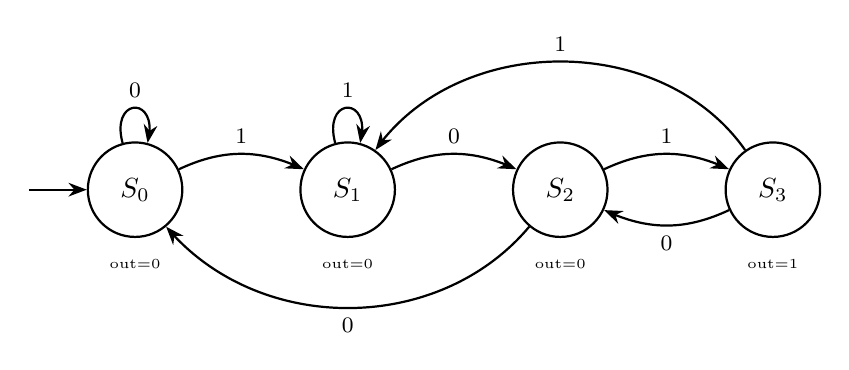
\begin{tikzpicture}[>=Stealth, scale=0.9]
  % States as circles
  \node[draw, circle, thick, minimum size=1.2cm] (S0) at (0,0) {$S_0$};
  \node[font=\tiny, below=0.15cm] at (S0.south) {out=0};
  \node[draw, circle, thick, minimum size=1.2cm] (S1) at (3,0) {$S_1$};
  \node[font=\tiny, below=0.15cm] at (S1.south) {out=0};
  \node[draw, circle, thick, minimum size=1.2cm] (S2) at (6,0) {$S_2$};
  \node[font=\tiny, below=0.15cm] at (S2.south) {out=0};
  \node[draw, circle, thick, minimum size=1.2cm] (S3) at (9,0) {$S_3$};
  \node[font=\tiny, below=0.15cm] at (S3.south) {out=1};
  
  % Initial arrow
  \draw[->, thick] (-1.5,0) -- (S0);
  
  % Transitions
  \draw[->, thick] (S0) to[bend left=25] node[above, font=\footnotesize]{1} (S1);
  \draw[->, thick] (S0) to[loop above, looseness=5] node[above, font=\footnotesize]{0} (S0);
  \draw[->, thick] (S1) to[bend left=25] node[above, font=\footnotesize]{0} (S2);
  \draw[->, thick] (S1) to[loop above, looseness=5] node[above, font=\footnotesize]{1} (S1);
  \draw[->, thick] (S2) to[bend left=25] node[above, font=\footnotesize]{1} (S3);
  \draw[->, thick] (S2) to[bend left=50] node[below, font=\footnotesize]{0} (S0);
  \draw[->, thick] (S3) to[bend left=25] node[below, font=\footnotesize]{0} (S2);
  \draw[->, thick] (S3) to[bend right=55] node[above, font=\footnotesize]{1} (S1);
\end{tikzpicture}
\end{center}

La machine détecte la séquence ``1-0-1'' dans un flux de bits. La sortie passe à 1 pendant un cycle quand la séquence complète est reconnue ($S_3$).
\end{formule}

\begin{retenir}
\textbf{L'essentiel :}
\begin{enumerate}[nosep]
\item FSM = ensemble fini d'états + transitions conditionnelles + sorties.
\item Moore : sorties = f(état). Stables. Standard en conception.
\item Mealy : sorties = f(état, entrées). Plus rapide mais glitches possibles.
\item Diagramme d'états : bulles (états) + flèches (transitions) = le ``plan'' de la machine.
\end{enumerate}
\end{retenir}

% ============================================================================
\section{Approfondissement}

\vspace{0.3cm}
\textit{Du diagramme d'états au circuit physique : comment implémenter une FSM avec des bascules D et de la logique combinatoire, et comment le timing contraint la conception.}
\vspace{0.3cm}

\begin{approfondissement}
Codage des états, implémentation physique, méthodologie complète de conception, et lien avec le timing. Prérequis : chapitres 20 (logique combinatoire, Karnaugh), 21 (bascules D, setup/hold), 22 (chemin critique, STA).
\end{approfondissement}

\subsection{L'implémentation physique : registre + nuage combinatoire}

\begin{formule}
\textbf{Toute FSM se décompose en deux blocs :}

\textbf{1. Le registre d'état} : $n$ bascules D qui stockent l'état courant, codé sur $n$ bits. Au front d'horloge, le registre capture l'état suivant calculé par la logique combinatoire.

\textbf{2. Le nuage combinatoire} : un bloc de logique combinatoire (portes NAND, NOR, MUX\ldots) qui calcule :
\begin{itemize}[nosep]
\item L'\textbf{état suivant} $D_k$ (entrées des bascules) en fonction de l'état courant $Q_k$ et des entrées $I$.
\item Les \textbf{sorties} $O$ en fonction de l'état courant seul (Moore) ou de l'état courant et des entrées (Mealy).
\end{itemize}
\end{formule}

\begin{center}
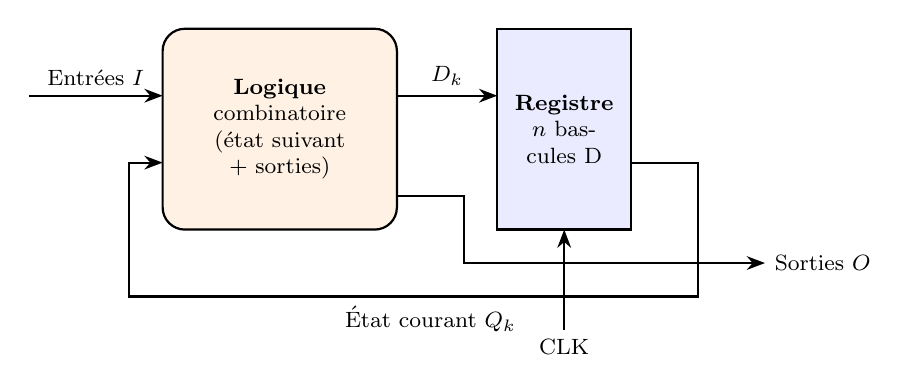
\begin{tikzpicture}[>=Stealth, scale=0.85]
  % Registre
  \draw[thick, fill=blue!8] (5,0) rectangle (7,3);
  \node[font=\footnotesize, text width=1.5cm, align=center] at (6,1.5) {\textbf{Registre}\\$n$ bascules D};
  
  % Nuage combinatoire
  \draw[thick, fill=orange!10, rounded corners=8pt] (0,0) rectangle (3.5,3);
  \node[font=\footnotesize, text width=3cm, align=center] at (1.75,1.5) {\textbf{Logique}\\combinatoire\\(état suivant\\+ sorties)};
  
  % Entrées
  \draw[->, thick] (-2,2) -- (0,2) node[midway, above, font=\footnotesize]{Entrées $I$};
  
  % Nuage -> Registre (état suivant)
  \draw[->, thick] (3.5,2) -- (5,2) node[midway, above, font=\footnotesize]{$D_k$};
  
  % Registre -> Nuage (rétroaction état courant)
  \draw[->, thick] (7,1) -- (8,1) -- (8,-1) -- (-0.5,-1) -- (-0.5,1) -- (0,1);
  \node[font=\footnotesize, below] at (4,-1) {État courant $Q_k$};
  
  % Horloge
  \draw[->, thick] (6,-1.5) -- (6,0);
  \node[font=\footnotesize, below] at (6,-1.5) {CLK};
  
  % Sorties
  \draw[->, thick] (3.5,0.5) -- (4.5,0.5) -- (4.5,-0.5) -- (9,-0.5);
  \node[font=\footnotesize, right] at (9,-0.5) {Sorties $O$};
\end{tikzpicture}
\end{center}

\begin{attention}
\textbf{Le timing de la FSM est directement lié au nuage combinatoire.}

Le délai du nuage combinatoire est le terme $t_{\text{comb}}$ dans la contrainte de timing (chapitre 22) :
\[
\boxed{T_{\text{clk}} \geq t_{cq} + t_{\text{comb}} + t_{su}}
\]

\textbf{Conséquence directe :}
\begin{itemize}[nosep]
\item Plus la FSM a d'états $\Rightarrow$ plus le codage est large ($n$ bits) $\Rightarrow$ plus la logique combinatoire est profonde $\Rightarrow$ $t_{\text{comb}} \uparrow$ $\Rightarrow$ $f_{\max} \downarrow$.
\item Plus les conditions de transition sont complexes (beaucoup d'entrées, conditions imbriquées) $\Rightarrow$ plus de niveaux logiques $\Rightarrow$ $t_{\text{comb}} \uparrow$.
\end{itemize}

\textbf{La vitesse d'une FSM est dictée par l'épaisseur du nuage combinatoire.} Simplifier les transitions ou changer le codage des états peut accélérer la machine.
\end{attention}

\subsection{Codage des états}

Le choix du codage des états a un impact direct sur la complexité du nuage combinatoire et donc sur la vitesse :

\begin{formule}
\textbf{Trois codages principaux :}

\begin{center}
\renewcommand{\arraystretch}{1.4}
\begin{tabular}{p{2.5cm}p{2cm}p{2.5cm}p{5.5cm}}
\toprule
\textbf{Codage} & \textbf{Bascules} & \textbf{Logique} & \textbf{Quand l'utiliser} \\
\midrule
\textbf{Binaire} & $\lceil\log_2 N\rceil$ & Complexe & ASIC avec peu de bascules disponibles \\
\textbf{Gray} & $\lceil\log_2 N\rceil$ & Moins de glitches & Compteurs, traversée de domaines \\
\textbf{One-hot} & $N$ & \textbf{Très simple} & \textbf{FPGA} (bascules abondantes, logique limitante) \\
\bottomrule
\end{tabular}
\end{center}
\end{formule}

\begin{intuition}
\textbf{Pourquoi le one-hot est le standard en FPGA :}

En codage one-hot, chaque état est représenté par une seule bascule à ``1'' (toutes les autres à ``0''). L'équation de transition de chaque bascule est très simple : $D_k = \sum(\text{transitions entrantes vers } S_k)$. Il n'y a pas besoin de décodeur pour identifier l'état courant (chaque bascule \textit{est} l'état). La logique combinatoire est \textbf{peu profonde} (1--2 niveaux de portes), donc $t_{\text{comb}}$ est minimal.

\textbf{Le prix :} $N$ bascules au lieu de $\lceil\log_2 N\rceil$. Mais dans un FPGA, les bascules sont abondantes (la ressource limitante est la logique combinatoire). En ASIC, le one-hot consomme plus de surface et n'est utilisé que si la vitesse est critique.
\end{intuition}

\subsection{Méthodologie complète de conception}

\begin{pratique}
\textbf{De la spécification au circuit --- 7 étapes :}

\textbf{Étape 1 --- Spécification.}
Décrire le comportement attendu en langage naturel : entrées, sorties, séquence d'opérations.

\textbf{Étape 2 --- Diagramme d'états.}
Dessiner les bulles (états) et les flèches (transitions). Vérifier : chaque état a-t-il une transition pour \textit{chaque} combinaison d'entrées ? (Sinon : état piégé.) Y a-t-il un chemin de reset vers l'état initial ?

\textbf{Étape 3 --- Choisir Moore ou Mealy.}
Moore par défaut. Mealy si la latence est critique.

\textbf{Étape 4 --- Coder les états.}
Binaire (ASIC), one-hot (FPGA), ou Gray (compteurs/CDC).

\textbf{Étape 5 --- Table de transition.}
Pour chaque état courant et chaque combinaison d'entrées : état suivant + sorties.

\textbf{Étape 6 --- Équations logiques.}
Déduire $D_k$ (entrée de chaque bascule) et les sorties par Karnaugh ou outil de synthèse. Vérifier les états ``don't care'' (états non utilisés en codage non-complet).

\textbf{Étape 7 --- Implémentation et vérification.}
Implémenter en HDL (VHDL ou Verilog) ou en portes discrètes. Simuler fonctionnellement puis vérifier le timing (STA, chapitre 22).
\end{pratique}

\subsection{Exemple complet : contrôleur de feu tricolore}

\begin{pratique}
\textbf{Spécification :} un feu de signalisation avec 4 phases : Vert ($\SI{30}{s}$), Orange ($\SI{5}{s}$), Rouge ($\SI{30}{s}$), Rouge+Orange ($\SI{2}{s}$, transition vers vert). Horloge de $\SI{1}{Hz}$ (1 tick par seconde). Entrée : aucune (séquence fixe). Sorties : R, O, V.

\textbf{Diagramme :} 4 états avec compteurs internes pour les durées. Machine de Moore.

\textbf{Codage one-hot :} 4 bascules ($S_V$, $S_O$, $S_R$, $S_{RO}$). Les sorties sont directement les bascules : $V = S_V$, $O = S_O \lor S_{RO}$, $R = S_R \lor S_{RO}$.

\textbf{Compteur de durée :} un compteur partagé de 5 bits (compte de 0 à 30). La transition vers l'état suivant se fait quand le compteur atteint la valeur programmée pour l'état courant.

\textbf{Logique de transition :}
\begin{itemize}[nosep]
\item $D_V = S_{RO} \cdot (\text{cnt} = 2)$ : on passe au Vert quand le compteur Rouge+Orange atteint 2.
\item $D_O = S_V \cdot (\text{cnt} = 30)$ : on passe à l'Orange quand le Vert a duré 30\,s.
\item $D_R = S_O \cdot (\text{cnt} = 5)$.
\item $D_{RO} = S_R \cdot (\text{cnt} = 30)$.
\end{itemize}
Chaque transition ne dépend que d'une bascule et d'un comparateur $\Rightarrow$ logique très simple, $t_{\text{comb}}$ minimal.
\end{pratique}

% ============================================================================
\section{Niveau Ingénieur}

\begin{ingenieur}
Optimisation de la FSM pour le timing, gestion des états invalides, reset, et FSM en HDL. Lien avec l'architecture des systèmes numériques.
\end{ingenieur}

\subsection{Optimisation du timing de la FSM}

\begin{formule}
La fréquence maximale d'une FSM est :
\[
f_{\max} = \frac{1}{t_{cq} + t_{\text{comb}} + t_{su}}
\]

\textbf{Stratégies d'optimisation de $t_{\text{comb}}$ :}
\begin{enumerate}[nosep]
\item \textbf{Codage one-hot} : réduit la profondeur logique (1--2 niveaux vs $\log_2 N$ niveaux en binaire).
\item \textbf{Décomposition de la FSM} : scinder une FSM complexe en deux FSM plus simples qui communiquent par des signaux de handshake. Chaque sous-FSM a un nuage combinatoire plus petit.
\item \textbf{Pipeline de sortie} : si les sorties sont complexes (décodage élaboré), insérer un registre entre la logique de sortie et les sorties physiques. Coût : +1 cycle de latence.
\item \textbf{Encodage des conditions} : si une transition dépend de $(A \cdot B \cdot C \cdot D)$, pré-calculer le produit dans un registre intermédiaire au cycle précédent.
\end{enumerate}
\end{formule}

\begin{pratique}
\textbf{Exemple chiffré :} FSM de contrôle mémoire avec 16 états (codage binaire : 4 bascules). La logique combinatoire a 5 niveaux de portes ($t_p = \SI{50}{ps}$/porte $\Rightarrow$ $t_{\text{comb}} = \SI{250}{ps}$). Avec $t_{cq} = \SI{50}{ps}$, $t_{su} = \SI{30}{ps}$ :

$f_{\max} = 1/(50+250+30) = 1/\SI{330}{ps} = \SI{3.03}{GHz}$.

En one-hot (16 bascules, 2 niveaux) : $t_{\text{comb}} = \SI{100}{ps}$. $f_{\max} = 1/\SI{180}{ps} = \SI{5.56}{GHz}$. Gain : $\times 1{,}8$.
\end{pratique}

\subsection{Gestion des états invalides}

\begin{attention}
\textbf{Le problème :} en codage binaire avec $n$ bascules, il y a $2^n$ états possibles mais seulement $N$ états valides ($N < 2^n$ en général). Si un bruit, une perturbation, ou un mauvais reset place la FSM dans un état \textbf{non prévu}, elle peut rester bloquée indéfiniment (état piégé) ou se comporter de manière dangereuse.

\textbf{Solutions (par ordre de robustesse) :}
\begin{enumerate}[nosep]
\item \textbf{Traiter les ``don't care'' avec précaution :} dans le Karnaugh, ne pas utiliser les états invalides comme ``don't care'' de manière agressive. S'assurer que les états invalides transitent vers un état valide (typiquement l'état initial) en au plus 1--2 cycles.
\item \textbf{Clause ``default'' en HDL :} dans le \texttt{case} de la FSM, toujours inclure un \texttt{default} $\Rightarrow$ état initial. C'est la règle n°1 en VHDL/Verilog.
\item \textbf{Watchdog :} un compteur indépendant qui reset la FSM si elle ne visite pas un état ``vivant'' dans un délai imparti. Utilisé dans les systèmes critiques (automobile, aéronautique).
\end{enumerate}
\end{attention}

\begin{intuition}
\textbf{En one-hot, le problème est différent :} les états invalides sont ceux où plusieurs bascules (ou aucune) sont à ``1''. La probabilité d'y tomber est plus élevée qu'en binaire (car il y a $2^N - N$ états invalides sur $2^N$ possibles, soit la quasi-totalité). La protection standard : un ``one-hot checker'' qui détecte si exactement une bascule est à ``1'' et reset sinon.
\end{intuition}

\subsection{Reset : synchrone vs asynchrone}

\begin{formule}
\textbf{Reset asynchrone :} le signal de reset force immédiatement les bascules à l'état initial, sans attendre le front d'horloge. Avantage : la FSM démarre dans un état connu dès la mise sous tension, même si l'horloge n'est pas encore stable.

\textbf{Reset synchrone :} le reset n'est pris en compte qu'au front d'horloge. Avantage : pas de risque de violation de timing (le reset est traité comme une entrée normale). Inconvénient : nécessite que l'horloge fonctionne.

\textbf{Meilleure pratique --- ``async assert, sync deassert'' :}
\begin{itemize}[nosep]
\item L'\textbf{assertion} du reset est asynchrone : la FSM se reset immédiatement.
\item La \textbf{désactivation} du reset passe par un synchroniseur (double bascule D dans le domaine d'horloge) : toutes les bascules sortent du reset \textbf{au même front d'horloge}.
\end{itemize}
Sans cette précaution, certaines bascules pourraient sortir du reset un cycle avant les autres, plaçant la FSM dans un état incohérent.
\end{formule}

\subsection{FSM en HDL : les bonnes pratiques}

\begin{pratique}
\textbf{Structure standard en VHDL/Verilog (style ``3 process'' ou ``2 always'') :}

\textbf{Bloc 1 --- Registre d'état} (séquentiel) :
\begin{itemize}[nosep]
\item Sensible au front d'horloge et au reset.
\item Capture l'état suivant : \texttt{state <= next\_state}.
\item C'est ici que vivent les bascules D.
\end{itemize}

\textbf{Bloc 2 --- Logique de transition} (combinatoire) :
\begin{itemize}[nosep]
\item Calcule \texttt{next\_state} en fonction de \texttt{state} et des entrées.
\item Structure \texttt{case/switch} avec \texttt{default} $\to$ état initial.
\end{itemize}

\textbf{Bloc 3 --- Logique de sortie} (combinatoire ou registrée) :
\begin{itemize}[nosep]
\item Moore : sorties = f(\texttt{state}) uniquement.
\item Mealy : sorties = f(\texttt{state}, entrées).
\item Optionnel : registre de sortie pour éliminer les glitches.
\end{itemize}

\textbf{Erreur classique :} oublier un cas dans le \texttt{case} $\Rightarrow$ le synthétiseur infère un \textbf{latch} (verrou) au lieu d'un registre. Cela crée un chemin combinatoire non voulu et potentiellement instable. \textbf{Toujours couvrir tous les cas ou mettre un \texttt{default}.}
\end{pratique}

\subsection{La FSM dans l'architecture des systèmes}

\begin{intuition}
\textbf{La FSM est partout dans un système numérique :}
\begin{itemize}[nosep]
\item \textbf{Contrôleur UART :} FSM qui gère la sérialisation des bits (start, data, parity, stop).
\item \textbf{Contrôleur SPI/I2C :} FSM qui pilote le protocole de communication.
\item \textbf{Contrôleur mémoire DDR :} FSM complexe avec $>30$ états pour gérer l'initialisation, le refresh, les commandes de lecture/écriture, et les timings stricts de la DRAM (lien chapitre 24).
\item \textbf{Pipeline de processeur :} chaque étage de pipeline (fetch, decode, execute, writeback) est une FSM qui coordonne le flux d'instructions.
\item \textbf{Arbitre de bus :} FSM qui décide quel maître a accès au bus à chaque cycle.
\end{itemize}

Dans un FPGA ou un ASIC complexe, il y a typiquement des \textbf{dizaines à centaines de FSM} qui fonctionnent en parallèle et communiquent entre elles par des signaux de handshake ou des FIFO (chapitre 22).
\end{intuition}

% === EXERCICES ===
\section*{Exercices}
\addcontentsline{toc}{section}{Exercices}

\subsection*{Niveau débutant}

\textbf{Exercice 23.1 ---} Dessinez le diagramme d'états d'une FSM de Moore qui détecte la séquence ``110'' dans un flux de bits (entrée : $X$, sortie : $Z = 1$ quand la séquence est détectée). Combien d'états faut-il ?

\begin{pratique}
\textbf{Solution :} 4 états : $S_0$ (initial, rien détecté), $S_1$ (un ``1'' reçu), $S_2$ (``11'' reçu), $S_3$ (``110'' détecté, $Z = 1$).

Transitions : $S_0 \xrightarrow{1} S_1$, $S_0 \xrightarrow{0} S_0$, $S_1 \xrightarrow{1} S_2$, $S_1 \xrightarrow{0} S_0$, $S_2 \xrightarrow{0} S_3$, $S_2 \xrightarrow{1} S_2$, $S_3 \xrightarrow{1} S_1$, $S_3 \xrightarrow{0} S_0$.

Sortie : $Z = 1$ seulement dans $S_3$.
\end{pratique}

\textbf{Exercice 23.2 ---} La même spécification en Mealy. Combien d'états faut-il ? Quel est l'avantage ?

\begin{pratique}
\textbf{Solution :} 3 états suffisent : $S_0$, $S_1$ (``1''), $S_2$ (``11''). La sortie $Z = 1$ est émise \textit{sur la transition} $S_2 \xrightarrow{0} S_0$ (et non dans un état dédié). Avantage : 1 état de moins. La sortie réagit immédiatement quand le ``0'' arrive, 1 cycle plus tôt que Moore.
\end{pratique}

\subsection*{Niveau intermédiaire}

\textbf{Exercice 23.3 ---} Implémentez la FSM de l'exercice 23.1 en bascules D avec codage binaire ($S_0 = 00$, $S_1 = 01$, $S_2 = 10$, $S_3 = 11$). Donnez les équations de $D_1$, $D_0$ et $Z$ par Karnaugh.

\begin{pratique}
\textbf{Solution :} Variables d'état $Q_1 Q_0$, entrée $X$.

Table de transition :
\begin{center}
\renewcommand{\arraystretch}{1.1}
\begin{tabular}{cc|c|cc|c}
\toprule
$Q_1$ & $Q_0$ & $X$ & $D_1$ & $D_0$ & $Z$ \\
\midrule
0 & 0 & 0 & 0 & 0 & 0 \\
0 & 0 & 1 & 0 & 1 & 0 \\
0 & 1 & 0 & 0 & 0 & 0 \\
0 & 1 & 1 & 1 & 0 & 0 \\
1 & 0 & 0 & 1 & 1 & 0 \\
1 & 0 & 1 & 1 & 0 & 0 \\
1 & 1 & 0 & 0 & 0 & 1 \\
1 & 1 & 1 & 0 & 1 & 1 \\
\bottomrule
\end{tabular}
\end{center}

Par Karnaugh : $D_1 = Q_0 X + Q_1\overline{X}$, $D_0 = \overline{Q_1}\,\overline{Q_0}\,X + Q_1\,\overline{X}$, $Z = Q_1 Q_0$.
\end{pratique}

\textbf{Exercice 23.4 ---} Reprenez l'exercice 23.3 en codage one-hot ($S_0$, $S_1$, $S_2$, $S_3$ = 4 bascules). Donnez les équations de $D_{S_0}$, $D_{S_1}$, $D_{S_2}$, $D_{S_3}$. Comparez la profondeur logique avec le codage binaire.

\begin{pratique}
\textbf{Solution :}

$D_{S_0} = S_0\,\overline{X} + S_1\,\overline{X} + S_3\,\overline{X}$ (transitions entrantes vers $S_0$).

$D_{S_1} = S_0\,X + S_3\,X$.

$D_{S_2} = S_1\,X$.

$D_{S_3} = S_2\,\overline{X}$.

$Z = S_3$.

Profondeur logique : chaque $D$ est une somme de produits de 2 termes (1 porte AND + 1 porte OR) = \textbf{2 niveaux}. En binaire : $D_1 = Q_0 X + Q_1\overline{X}$ est aussi 2 niveaux, mais les conditions deviennent plus profondes si le nombre d'états augmente (décodage de l'état courant en $\lceil\log_2 N\rceil$ bits).
\end{pratique}

\subsection*{Niveau ingénieur}

\textbf{Exercice 23.5 ---} Une FSM de contrôle mémoire a 24 états en codage binaire (5 bascules). La logique combinatoire a 6 niveaux de portes ($t_p = \SI{40}{ps}$/porte). $t_{cq} = \SI{45}{ps}$, $t_{su} = \SI{25}{ps}$.

(a) Quelle est la fréquence maximale ?

(b) En passant en one-hot (24 bascules, 2 niveaux), quelle est la nouvelle $f_{\max}$ ?

(c) Si on décompose la FSM en 2 sous-FSM de 12 états chacune (codage binaire, 4 bascules, 4 niveaux), quel est le gain ?

\begin{pratique}
\textbf{Solution :}

(a) $t_{\text{comb}} = 6\times40 = \SI{240}{ps}$. $T_{\min} = 45+240+25 = \SI{310}{ps}$. $f_{\max} = \SI{3.23}{GHz}$.

(b) One-hot : $t_{\text{comb}} = 2\times40 = \SI{80}{ps}$. $T_{\min} = 45+80+25 = \SI{150}{ps}$. $f_{\max} = \SI{6.67}{GHz}$. Gain : $\times 2{,}1$.

(c) Décomposée : $t_{\text{comb}} = 4\times40 = \SI{160}{ps}$. $T_{\min} = 45+160+25 = \SI{230}{ps}$. $f_{\max} = \SI{4.35}{GHz}$. Gain : $\times 1{,}35$ par rapport au monolithique, mais avec seulement $2\times4 = 8$ bascules (vs 24 en one-hot).
\end{pratique}

\textbf{Exercice 23.6 ---} Un synthétiseur génère une FSM en one-hot avec 32 états dans un FPGA. Après place \& route, le rapport de timing indique un slack de $\SI{-0.2}{ns}$ à $\SI{200}{MHz}$. Que faire ?

\begin{pratique}
\textbf{Solution :} slack négatif = violation de timing. Options par ordre de préférence :

\textbf{1.} Vérifier si le chemin critique traverse la FSM. Si oui : pré-calculer les conditions de transition complexes dans un registre intermédiaire (technique du ``flag register'' : calculer la condition au cycle $n-1$ et la mémoriser pour le cycle $n$).

\textbf{2.} Décomposer la FSM en sous-FSM plus simples.

\textbf{3.} Registrer les sorties (ajouter un étage de pipeline).

\textbf{4.} Si rien ne suffit : réduire la fréquence à $1/(T_{\text{clk}} + |slack|) = 1/(5+0{,}2) = \SI{192}{MHz}$, ou utiliser un FPGA de speed grade supérieur.
\end{pratique}

\subsection*{Questions de compréhension}

\begin{enumerate}[nosep]
\item Pourquoi le codage one-hot produit-il une logique combinatoire moins profonde que le codage binaire ? Reliez votre réponse au fait qu'en one-hot, identifier l'état courant ne nécessite aucun décodage.
\item Une FSM de Mealy peut produire des glitches sur ses sorties. Pourquoi ? Comment les éliminer sans revenir à une machine de Moore ?
\item Expliquez pourquoi l'inférence d'un latch dans une FSM en HDL est un bug grave. Quel est l'impact sur le timing et la fiabilité ?
\item Un contrôleur DDR4 a 48 états. En codage binaire (6 bascules), la logique de transition a 8 niveaux de portes. En one-hot, elle en a 2. Pourquoi ne choisit-on pas toujours le one-hot ?
\end{enumerate}

% === RÉSUMÉ ===
\section*{Résumé du chapitre}
\addcontentsline{toc}{section}{Résumé du chapitre}

\begin{bases}[title={\color{white} Résumé --- Les Bases}]
\begin{center}
\renewcommand{\arraystretch}{1.3}
\begin{tabular}{p{3.5cm}p{9.5cm}}
\toprule
FSM & États finis + transitions + sorties. Modèle universel du séquentiel \\
Moore & Sorties = f(état). Stables. Standard en conception \\
Mealy & Sorties = f(état, entrées). Plus rapide, glitches possibles \\
Diagramme d'états & Bulles (états) + flèches (transitions) = le plan de la machine \\
\bottomrule
\end{tabular}
\end{center}
\end{bases}

\begin{approfondissement}[title={\color{white} Résumé --- Approfondissement}]
\begin{center}
\renewcommand{\arraystretch}{1.3}
\begin{tabular}{p{3.5cm}p{9.5cm}}
\toprule
Implémentation & Registre d'état ($n$ bascules D) + nuage combinatoire \\
$f_{\max}$ & $= 1/(t_{cq} + t_{\text{comb}} + t_{su})$. \textbf{Vitesse $=$ épaisseur du nuage} \\
Codage & Binaire (compact), one-hot (rapide, FPGA), Gray (compteurs) \\
Conception & Spéc $\to$ diagramme $\to$ codage $\to$ table $\to$ Karnaugh $\to$ HDL $\to$ STA \\
\bottomrule
\end{tabular}
\end{center}
\end{approfondissement}

\begin{ingenieur}[title={\color{white} Résumé --- Niveau Ingénieur}]
\begin{center}
\renewcommand{\arraystretch}{1.3}
\begin{tabular}{p{3.5cm}p{9.5cm}}
\toprule
Optimisation & One-hot, décomposition, pipeline de sortie, pré-calcul des conditions \\
États invalides & Traiter les ``don't care'' prudemment, clause \texttt{default}, watchdog \\
Reset & Async assert, sync deassert. Toutes les bascules sortent de reset ensemble \\
HDL & 3 blocs (registre, transition, sortie). Toujours couvrir tous les cas (\texttt{default}) \\
\bottomrule
\end{tabular}
\end{center}
\end{ingenieur}

% ============================================================================
% CHAPITRE 24 : MÉMOIRE — DU BIT PHYSIQUE AU SYSTÈME
% ============================================================================
% ============================================================================
% CHAPITRE 24 : MÉMOIRE — DU BIT PHYSIQUE AU SYSTÈME
% VERSION PEER-REVIEW
% Fichier autonome à intégrer dans Bible_Elec.tex
% ============================================================================

\chapter{Mémoire : du bit physique au système}

\begin{center}
\textit{Stocker un bit d'information semble trivial.\\
En réalité, c'est un défi de physique analogique déguisé en numérique :\\
maintenir une charge sur un condensateur qui fuit,\\
stabiliser une boucle de rétroaction qui peut basculer,\\
ou piéger des électrons dans un oxyde pendant des années.\\
Chaque type de mémoire est un compromis différent\\
entre vitesse, densité, consommation et rétention.}
\end{center}

\vspace{0.5cm}

Les chapitres précédents ont utilisé les bascules D comme éléments de mémoire. Mais une bascule D occupe 20 à 40 transistors : stocker un gigaoctet en bascules est impossible. Ce chapitre explore les trois technologies fondamentales de mémoire --- SRAM, DRAM et Flash --- en partant du mécanisme physique qui stocke le bit, pour comprendre les limites de chaque technologie et pourquoi on les utilise ensemble dans les systèmes modernes.

\begin{intuition}
\textbf{Le fil conducteur de ce chapitre :} toute mémoire numérique repose sur un phénomène \textbf{analogique}. Un ``1'' ou un ``0'' est physiquement une tension, un courant, ou une charge --- des grandeurs continues, soumises au bruit, aux fuites et à la température. La frontière entre ``se souvenir'' et ``oublier'' est une question de physique, pas de logique.
\end{intuition}

% ============================================================================
\section{Les Bases}

\begin{bases}
Les trois mécanismes physiques fondamentaux de stockage d'un bit : rétroaction (SRAM), charge capacitive (DRAM), et piégeage de charge (Flash). Prérequis : chapitres 17 (MOSFET), 20 (CMOS), 21 (verrou SR, bascule D).
\end{bases}

\subsection{Trois façons de stocker un bit}

\begin{formule}
\begin{center}
\renewcommand{\arraystretch}{1.5}
\begin{tabular}{p{2cm}p{3.5cm}p{3cm}p{4cm}}
\toprule
\textbf{Type} & \textbf{Mécanisme physique} & \textbf{Rétention} & \textbf{Usage principal} \\
\midrule
\textbf{SRAM} & Rétroaction croisée (2 inverseurs) & Tant que $V_{DD}$ est présente (volatile) & Cache processeur, registres \\
\textbf{DRAM} & Charge sur un condensateur & Quelques ms (volatile, fuite) & Mémoire principale (RAM) \\
\textbf{Flash} & Électrons piégés dans un oxyde & Années (non volatile) & Stockage (SSD, clé USB, firmware) \\
\bottomrule
\end{tabular}
\end{center}
\end{formule}

\begin{intuition}
\textbf{Le compromis fondamental :}
\begin{itemize}[nosep]
\item \textbf{SRAM} : la plus rapide ($\sim\SI{1}{ns}$) mais la plus volumineuse (6 transistors par bit).
\item \textbf{DRAM} : densité élevée (1 transistor + 1 condensateur par bit) mais lente ($\sim\SI{10}{ns}$--$\SI{50}{ns}$) et nécessite un rafraîchissement permanent.
\item \textbf{Flash} : non volatile (conserve les données sans alimentation) mais écriture très lente ($\sim\SI{1}{ms}$), usure en écriture, et endurance limitée ($10^3$--$10^5$ cycles).
\end{itemize}
Aucune technologie ne satisfait tout : c'est pourquoi les systèmes utilisent une \textbf{hiérarchie} de mémoires (registres $\to$ cache SRAM $\to$ RAM DRAM $\to$ stockage Flash/SSD).
\end{intuition}

\subsection{La SRAM : la mémoire par rétroaction}

La cellule SRAM est un \textbf{verrou croisé} : deux inverseurs CMOS connectés tête-bêche, formant une boucle de rétroaction positive qui maintient un état binaire stable.

\begin{center}
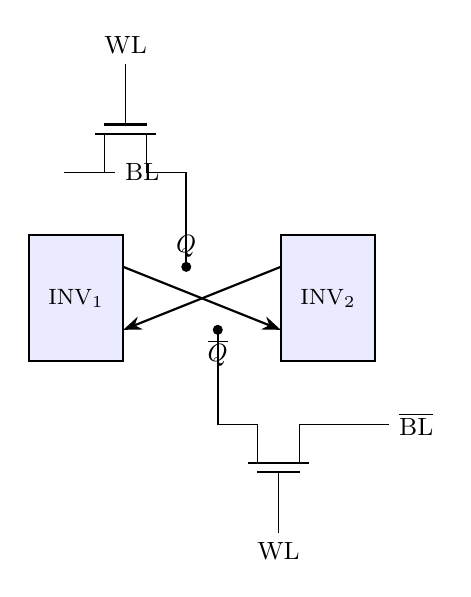
\begin{tikzpicture}[scale=0.8, >=Stealth]
  % Inverseur 1
  \draw[thick, fill=blue!8] (0,0) rectangle (1.5,2);
  \node[font=\footnotesize] at (0.75,1) {INV$_1$};
  % Inverseur 2
  \draw[thick, fill=blue!8] (4,0) rectangle (5.5,2);
  \node[font=\footnotesize] at (4.75,1) {INV$_2$};
  % Rétroaction croisée
  \draw[->, thick] (1.5,1.5) -- (4,0.5);
  \draw[->, thick] (4,1.5) -- (1.5,0.5);
  % Noeud Q
  \filldraw (2.5,1.5) circle (2pt);
  \node[above, font=\small] at (2.5,1.5) {$Q$};
  % Noeud Qbar
  \filldraw (3,0.5) circle (2pt);
  \node[below, font=\small] at (3,0.5) {$\overline{Q}$};
  % Transistors d'accès
  \draw[thick] (2.5,1.5) -- (2.5,3);
  \draw (2.5,3) node[nmos, anchor=S, rotate=90, xscale=-1](T1){};
  \draw (T1.D) -- ++(0.8,0) node[right, font=\small]{BL};
  \draw (T1.G) -- ++(0,0.5) node[above, font=\small]{WL};
  %
  \draw[thick] (3,0.5) -- (3,-1);
  \draw (3,-1) node[nmos, anchor=D, rotate=90](T2){};
  \draw (T2.S) -- ++(0.8,0) node[right, font=\small]{$\overline{\text{BL}}$};
  \draw (T2.G) -- ++(0,-0.5) node[below, font=\small]{WL};
\end{tikzpicture}
\end{center}

\begin{formule}
\textbf{Structure : la cellule 6T.}

\begin{itemize}[nosep]
\item 4 transistors pour les 2 inverseurs croisés (stockage).
\item 2 transistors d'accès (NMOS) commandés par la \textbf{ligne de mot} (WL, \textit{word line}).
\item 2 \textbf{lignes de bit} (BL, $\overline{\text{BL}}$) : paire différentielle qui transporte la donnée.
\end{itemize}

\textbf{Lecture :} WL passe à ``1'' $\Rightarrow$ les transistors d'accès connectent $Q$ et $\overline{Q}$ aux lignes BL et $\overline{\text{BL}}$. Un \textbf{amplificateur de détection} (\textit{sense amplifier}) mesure la \textit{différence} de tension entre BL et $\overline{\text{BL}}$ (quelques dizaines de mV) et l'amplifie en un signal logique complet.

\textbf{Écriture :} on force BL et $\overline{\text{BL}}$ aux niveaux complémentaires souhaités, puis on active WL. Les drivers de BL doivent être plus forts que les inverseurs internes pour ``retourner'' le verrou.
\end{formule}

\begin{attention}
\textbf{La SRAM est une mémoire volatile.} L'état se maintient tant que $V_{DD}$ est présente (les inverseurs consomment un courant de fuite $I_{\text{off}}$, chapitre 17). Sans alimentation, les tensions internes chutent et l'information est perdue. C'est le même phénomène que le verrou SR du chapitre 21 : la mémoire est \textbf{entretenue par l'alimentation}, pas par un stockage physique de charge.
\end{attention}

\subsection{La DRAM : la mémoire par stockage de charge}

\begin{formule}
\textbf{Structure : la cellule 1T1C.}

La cellule DRAM est radicalement plus simple : \textbf{un seul transistor} (accès) et \textbf{un condensateur} (stockage).

\begin{itemize}[nosep]
\item Un ``1'' est stocké comme une charge $Q = C \cdot V_{DD}$ sur le condensateur ($C \sim \SI{20}{fF}$--$\SI{30}{fF}$).
\item Un ``0'' est l'absence de charge ($Q = 0$).
\end{itemize}

\textbf{Lecture :} WL active le transistor d'accès $\Rightarrow$ la charge du condensateur se partage avec la capacité de la ligne de bit ($C_{BL} \gg C_{\text{cell}}$, typiquement $C_{BL} \sim 10\times C_{\text{cell}}$). La variation de tension sur BL est très faible :
\[
\Delta V_{BL} = \frac{C_{\text{cell}}}{C_{\text{cell}} + C_{BL}} \cdot V_{DD} \approx \frac{C_{\text{cell}}}{C_{BL}} \cdot V_{DD} \sim \SI{100}{mV}
\]
Un \textbf{sense amplifier} (rétroaction positive, essentiellement un verrou SR) amplifie ce $\SI{100}{mV}$ en un signal logique complet.

\textbf{La lecture est destructive :} le partage de charge vide partiellement le condensateur. Après chaque lecture, il faut \textbf{réécrire} la donnée (``restore'').
\end{formule}

\begin{attention}
\textbf{Le problème fondamental de la DRAM : la fuite.}

Le condensateur de stockage fuit à cause :
\begin{itemize}[nosep]
\item Du courant de fuite sub-seuil ($I_{\text{off}}$) du transistor d'accès (chapitre 17 : $I_{\text{off}}$ double tous les $\SI{10}{°C}$).
\item Du courant de fuite de la jonction PN (diode parasite du transistor d'accès).
\item Du courant de fuite à travers le diélectrique du condensateur.
\end{itemize}

Un condensateur de $\SI{20}{fF}$ chargé à $\SI{1}{V}$ stocke $Q = \SI{20}{fC}$. Avec un courant de fuite total de $\sim\SI{1}{fA}$, la charge se vide en $\tau = Q/I = \SI{20}{s}$. Mais la marge de détection du sense amplifier impose de lire \textit{avant} que la tension ne chute de plus de $\sim 30\%$ $\Rightarrow$ temps de rétention réel $\sim\SI{64}{ms}$.

\textbf{Solution : le rafraîchissement} (\textit{refresh}). Toutes les $\SI{64}{ms}$ (standard JEDEC), \textbf{chaque ligne} de la DRAM doit être lue et réécrite, même si personne ne la demande. Le refresh consomme de l'énergie et de la bande passante mémoire ($\sim 5\%$--$10\%$ du débit total).
\end{attention}

\subsection{La Flash : la mémoire par piégeage de charge}

\begin{formule}
\textbf{Structure : le transistor à grille flottante.}

La cellule Flash est un MOSFET modifié avec \textbf{deux grilles} :
\begin{itemize}[nosep]
\item La \textbf{grille flottante} (\textit{floating gate}) : une couche conductrice (polysilicium) isolée de toutes parts par un oxyde ($\text{SiO}_2$). Les électrons piégés dans cette grille y restent \textbf{des années} sans alimentation.
\item La \textbf{grille de contrôle} (\textit{control gate}) : la grille externe, connectée au circuit de commande.
\end{itemize}

\textbf{Stockage :} la présence ou l'absence d'électrons dans la grille flottante modifie la \textbf{tension de seuil} $V_{th}$ du MOSFET :
\begin{itemize}[nosep]
\item Grille flottante \textbf{chargée} (électrons piégés) : $V_{th} \uparrow$. Le transistor est plus difficile à ouvrir $\Rightarrow$ ``0'' (convention courante).
\item Grille flottante \textbf{vide} : $V_{th}$ nominal $\Rightarrow$ ``1''.
\end{itemize}

\textbf{Lecture :} on applique une tension intermédiaire sur la grille de contrôle ($V_{th,0} < V_G < V_{th,1}$). Si le transistor conduit : la grille flottante est vide (``1''). Si non : chargée (``0'').
\end{formule}

\begin{formule}
\textbf{Écriture (programmation) :} on applique une tension élevée ($\SI{15}{V}$--$\SI{20}{V}$) sur la grille de contrôle. Les électrons traversent l'oxyde par \textbf{effet tunnel de Fowler-Nordheim} ou par \textbf{injection de porteurs chauds} (\textit{hot carrier injection}, chapitre 17) et se retrouvent piégés dans la grille flottante.

\textbf{Effacement :} on applique une tension élevée inversée pour extraire les électrons. L'effacement se fait par \textbf{bloc entier} (d'où le nom ``Flash'' : effacement éclair de tout un secteur), pas bit par bit.

\textbf{Endurance :} chaque cycle d'écriture/effacement dégrade l'oxyde tunnel (création de pièges). Après $10^3$ à $10^5$ cycles, l'oxyde est trop dégradé pour retenir les électrons $\Rightarrow$ \textbf{usure}. Les contrôleurs SSD utilisent le ``wear leveling'' pour répartir les écritures.
\end{formule}

\begin{retenir}
\textbf{L'essentiel :}
\begin{enumerate}[nosep]
\item SRAM = 2 inverseurs croisés. Rapide, volatile, volumineuse (6T). Pour les caches.
\item DRAM = 1 transistor + 1 condensateur. Dense, volatile, fuit $\Rightarrow$ refresh toutes les $\SI{64}{ms}$. Pour la RAM.
\item Flash = grille flottante. Non volatile, lente en écriture, usure. Pour le stockage.
\item Toute mémoire numérique est un phénomène analogique (tension, charge, courant de fuite).
\end{enumerate}
\end{retenir}

% ============================================================================
\section{Approfondissement}

\vspace{0.3cm}
\textit{Les détails de conception qui séparent un bit qui fonctionne d'un bit qui échoue : stabilité de la SRAM, timing de la DRAM, et mémoire multi-niveaux en Flash.}
\vspace{0.3cm}

\begin{approfondissement}
Stabilité de la cellule SRAM (SNM), architecture DRAM (timing, refresh), et Flash multi-niveaux (MLC/TLC/QLC). Prérequis : section précédente, chapitre 17 (MOSFET, $I_{\text{off}}$).
\end{approfondissement}

\subsection{Stabilité de la cellule SRAM : la marge de bruit statique}

\begin{formule}
La \textbf{marge de bruit statique} (SNM, \textit{Static Noise Margin}) mesure la robustesse du verrou croisé : c'est la perturbation maximale que la cellule peut tolérer sans basculer d'état.

On la mesure en traçant les VTC des deux inverseurs ($V_{\text{out,1}}(V_{\text{in,1}})$ et $V_{\text{out,2}}(V_{\text{in,2}})$) l'une contre l'autre. Les deux courbes forment un ``papillon'' (\textit{butterfly curve}). La SNM est le côté du plus grand carré inscrit dans chaque lobe.

\textbf{Dégradation de la SNM :}
\begin{itemize}[nosep]
\item \textbf{$V_{DD} \downarrow$} : le gain des inverseurs diminue, les lobes du papillon se rétrécissent. En dessous d'un $V_{DD}$ critique ($\sim \SI{0.3}{V}$--$\SI{0.5}{V}$ selon la techno), la SNM tombe à zéro et la cellule ne tient plus.
\item \textbf{Température $\uparrow$} : $V_{th} \downarrow$ et $I_{\text{off}} \uparrow$ (chapitre 17), ce qui déséquilibre le verrou et réduit la SNM.
\item \textbf{Variabilité de fabrication} : en technologie avancée ($< \SI{14}{nm}$), les variations aléatoires de $V_{th}$ entre transistors (RDF, \textit{Random Dopant Fluctuation}) peuvent créer des cellules faibles dont la SNM est insuffisante. C'est le facteur limitant de la densité SRAM.
\end{itemize}
\end{formule}

\begin{intuition}
\textbf{Le gain de l'inverseur est la clé :} la SNM est directement liée au gain en tension des inverseurs CMOS dans la zone de transition (la VTC du chapitre 20). Un gain élevé $\Rightarrow$ lobes du papillon larges $\Rightarrow$ SNM élevée. En réduisant $V_{DD}$, le gain diminue et la cellule devient fragile. C'est le même mécanisme de ``restauration du signal'' que pour la logique combinatoire, mais ici il détermine si un bit est \textit{conservé} ou \textit{perdu}.
\end{intuition}

\subsection{Architecture et timing de la DRAM}

\begin{formule}
\textbf{Organisation d'une puce DRAM :}

La mémoire est organisée en une \textbf{matrice} de cellules 1T1C. L'accès se fait en deux phases :
\begin{enumerate}[nosep]
\item \textbf{RAS} (\textit{Row Access Strobe}) : active une ligne (WL). Les condensateurs de toute la ligne partagent leur charge avec les lignes de bit. Les sense amplifiers détectent et amplifient les données.
\item \textbf{CAS} (\textit{Column Access Strobe}) : sélectionne la colonne (le bit ou le groupe de bits) parmi la ligne activée. La donnée est envoyée sur le bus de données.
\end{enumerate}

\textbf{Paramètres de timing :}
\begin{itemize}[nosep]
\item $t_{\text{RCD}}$ (\textit{RAS to CAS Delay}) : délai entre l'activation de la ligne et la sélection de la colonne. Typiquement $\SI{10}{ns}$--$\SI{15}{ns}$.
\item $t_{\text{RP}}$ (\textit{Row Precharge}) : temps pour ``refermer'' une ligne et pré-charger les BL pour le prochain accès.
\item $t_{\text{RAS}}$ : durée minimale d'activation de la ligne.
\item $t_{\text{RFC}}$ (\textit{Refresh Cycle time}) : durée d'un cycle de rafraîchissement complet.
\end{itemize}

\textbf{Latence totale d'un accès aléatoire :}
\[
t_{\text{accès}} = t_{\text{RP}} + t_{\text{RCD}} + t_{\text{CAS}} \approx \SI{30}{ns}\text{--}\SI{50}{ns}
\]
soit $\sim 100$ cycles d'horloge à $\SI{3}{GHz}$. C'est pourquoi le cache (SRAM, $\sim\SI{1}{ns}$) est indispensable : il masque cette latence pour les données fréquemment utilisées.
\end{formule}

\begin{attention}
\textbf{Le refresh consomme de la bande passante.}

Standard JEDEC DDR4 : toutes les lignes doivent être rafraîchies toutes les $\SI{64}{ms}$. Pour une puce de $\SI{8}{Gb}$ avec $2^{17}$ lignes : $2^{17}/64\times10^{-3} = 2048$ refresh par ms, soit un refresh toutes les $\SI{488}{ns}$.

Chaque refresh occupe le bus pendant $t_{\text{RFC}} \approx \SI{260}{ns}$ (DDR4). Bande passante perdue : $260/488 = 53\%$ $\ldots$ Non : les refreshes sont répartis dans le temps (``distributed refresh''). En pratique, $\sim 5\%$--$10\%$ de la bande passante est perdue au refresh.

À haute température ($> \SI{85}{°C}$), les fuites augmentent exponentiellement et la fréquence de refresh doit \textbf{doubler} (passage à $\SI{32}{ms}$). Les serveurs en datacenter doivent prévoir cette pénalité.
\end{attention}

\subsection{Flash multi-niveaux : stocker plus de bits par cellule}

\begin{formule}
\textbf{SLC, MLC, TLC, QLC :}

Au lieu de stocker 1 bit par cellule (SLC, \textit{Single-Level Cell} : 2 niveaux de $V_{th}$), on peut stocker plusieurs bits en distinguant plus de niveaux de tension :

\begin{center}
\renewcommand{\arraystretch}{1.3}
\begin{tabular}{lcccc}
\toprule
\textbf{Type} & \textbf{Bits/cellule} & \textbf{Niveaux de $V_{th}$} & \textbf{Endurance} & \textbf{Vitesse lecture} \\
\midrule
SLC & 1 & 2 & $10^5$ cycles & $\SI{25}{\micro s}$ \\
MLC & 2 & 4 & $10^4$ & $\sim\SI{50}{\micro s}$ \\
TLC & 3 & 8 & $10^3$ & $\sim\SI{75}{\micro s}$ \\
QLC & 4 & 16 & $10^3$ & $\sim\SI{100}{\micro s}$ \\
\bottomrule
\end{tabular}
\end{center}
\end{formule}

\begin{attention}
\textbf{Le prix de la densité :} plus on met de niveaux, plus la \textbf{marge entre niveaux} diminue. En QLC (16 niveaux sur une fenêtre de $\sim\SI{4}{V}$), chaque niveau n'a qu'une marge de $\sim\SI{250}{mV}$. Le bruit (bruit thermique, perturbation des cellules voisines, usure de l'oxyde) peut facilement déplacer un niveau et corrompre le bit. C'est pourquoi les SSD QLC utilisent des \textbf{codes correcteurs d'erreur} (ECC) très puissants (LDPC : $\sim 100$ bits de parité pour 1 kbit de données) et un cache SLC interne pour les écritures rapides.
\end{attention}

% ============================================================================
\section{Niveau Ingénieur}

\begin{ingenieur}
Limites physiques fondamentales, scaling des mémoires, et technologies émergentes. Lien avec la physique des semi-conducteurs (chapitres 16--17) et les contraintes de conception.
\end{ingenieur}

\subsection{Les limites physiques de la DRAM}

\begin{formule}
Le scaling de la DRAM est limité par deux lois physiques :

\textbf{1. Le condensateur ne scale pas.}

La capacité doit rester $\geq \SI{15}{fF}$--$\SI{20}{fF}$ pour que le signal ($\Delta V_{BL}$) dépasse le bruit du sense amplifier. Quand la surface de la cellule diminue, il faut des condensateurs de plus en plus \textbf{grands en hauteur} (structures ``trench'' puis ``stack'' avec des rapports d'aspect $> 50:1$) ou des diélectriques à haute permittivité ($\text{HfO}_2$, $\varepsilon_r \sim 25$ vs $\varepsilon_r \sim 3{,}9$ pour $\text{SiO}_2$).

\textbf{2. Le courant de fuite augmente.}

En réduisant la longueur de grille du transistor d'accès, $I_{\text{off}}$ augmente exponentiellement (chapitre 17). Plus de fuite $=$ refresh plus fréquent $=$ plus de bande passante perdue.

\textbf{Conséquence :} le pitch des cellules DRAM stagne autour de $\sim\SI{15}{nm}$--$\SI{20}{nm}$ depuis $\sim 2015$. La densité progresse désormais par empilement vertical (HBM : \textit{High Bandwidth Memory}, jusqu'à 12 couches de dies empilés) plutôt que par réduction de la surface.
\end{formule}

\subsection{Les limites physiques de la Flash NAND}

\begin{formule}
\begin{itemize}[nosep]
\item \textbf{Épaisseur de l'oxyde tunnel :} si l'oxyde est trop mince ($< \SI{6}{nm}$), les électrons s'échappent par courant tunnel direct $\Rightarrow$ perte de données. L'oxyde tunnel ne peut plus être réduit.
\item \textbf{Nombre d'électrons par grille flottante :} en technologie planaire \SI{15}{nm}, la grille flottante ne contient que $\sim 100$ électrons pour un ``1'' programmé. La perte de $10$--$20$ électrons (par fuite ou perturbation) peut corrompre le bit.
\item \textbf{Couplage entre cellules :} les cellules adjacentes sont si proches que la charge de l'une influence le $V_{th}$ de l'autre (couplage capacitif parasite). C'est le ``program disturb''.
\end{itemize}

\textbf{Solution : la Flash 3D NAND.} Au lieu de réduire la surface, on empile les cellules verticalement (jusqu'à 232 couches en 2024). Chaque couche utilise un transistor relativement ``gros'' ($\sim\SI{40}{nm}$), ce qui restaure les marges physiques.
\end{formule}

\subsection{Le sense amplifier : l'interface analogique-numérique}

\begin{formule}
Le \textbf{sense amplifier} est le circuit critique qui fait le lien entre la physique analogique de la cellule mémoire et le monde numérique. C'est essentiellement un verrou SR (chapitre 21) avec un gain très élevé, conçu pour amplifier une différence de tension de $\sim\SI{50}{mV}$--$\SI{200}{mV}$ en un signal rail-à-rail ($0$ à $V_{DD}$) en un temps très court ($\sim\SI{1}{ns}$).

\textbf{Le sens amplifier de la DRAM est un amplificateur analogique :}
\begin{itemize}[nosep]
\item Il doit détecter une charge de $\sim\SI{20}{fC}$ sur un fond de bruit de $\sim\SI{5}{fC}$ (rapport signal/bruit $\sim 4$).
\item Son offset de transistor (dû aux variations de $V_{th}$, chapitre 17) doit être $< \SI{30}{mV}$, sinon il lit le bit à l'envers.
\item Sa vitesse est limitée par le $g_m$ des transistors internes et la capacité de BL (même compromis $g_m/C$ que l'AOP, chapitre 18).
\end{itemize}
\end{formule}

\begin{intuition}
\textbf{La mémoire, c'est de l'analogique déguisé :} le sense amplifier est un amplificateur différentiel (comme la paire d'entrée d'un AOP, chapitre 18). La cellule DRAM est un condensateur qui fuit (comme un intégrateur RC, chapitre 9). La cellule Flash est un MOSFET dont le $V_{th}$ est modifiable (chapitre 17). Toute la ``magie'' du numérique repose sur une couche de physique analogique invisible mais fondamentale.
\end{intuition}

\subsection{Effets thermiques et fiabilité}

\begin{formule}
\begin{itemize}[nosep]
\item \textbf{Température $\uparrow$ $\Rightarrow$ fuites $\uparrow$} (DRAM, SRAM). $I_{\text{off}} \times 2$ par $\SI{10}{°C}$ (chapitre 17). En DRAM : refresh plus fréquent. En SRAM : SNM dégradée.
\item \textbf{Rétention Flash $\downarrow$ avec $T$} : les électrons piégés dans la grille flottante ont plus d'énergie thermique et s'échappent plus facilement. La rétention passe de $> 10$ ans à \SI{25}{°C} à $\sim 1$ an à \SI{85}{°C} pour une Flash usée.
\item \textbf{Soft errors} (erreurs logiques transitoires) : un rayon cosmique ou une particule alpha (émise par les matériaux d'encapsulation) peut déposer assez de charge pour retourner un bit en SRAM ou DRAM. Taux : $\sim 1$ bit flip par $\SI{1}{Gb}$ par $\SI{1000}{h}$ au niveau de la mer. Les serveurs utilisent des DRAM ECC (1 bit de parité pour 8 bits de données) pour détecter et corriger ces erreurs.
\end{itemize}
\end{formule}

% === EXERCICES ===
\section*{Exercices}
\addcontentsline{toc}{section}{Exercices}

\subsection*{Niveau débutant}

\textbf{Exercice 24.1 ---} Un condensateur DRAM de $\SI{20}{fF}$ est chargé à $\SI{1}{V}$. Le courant de fuite total est $\SI{2}{fA}$. Combien de temps faut-il pour que la tension chute de $30\%$ ? Comparez avec l'intervalle de refresh standard de $\SI{64}{ms}$.

\begin{pratique}
\textbf{Solution :} $\Delta V = 30\% \times 1 = \SI{0.3}{V}$. $\Delta Q = C \times \Delta V = 20\times10^{-15}\times0{,}3 = \SI{6}{fC}$. $t = \Delta Q/I = 6\times10^{-15}/2\times10^{-15} = \SI{3}{s}$.

Le refresh à $\SI{64}{ms}$ a une marge de $3000/64 \approx 47\times$. Cette marge absorbe les pires cas (haute température, fuites exacerbées, cellules faibles).
\end{pratique}

\textbf{Exercice 24.2 ---} Une puce SRAM de $\SI{4}{Mb}$ utilise des cellules 6T. Combien de transistors contient-elle (cellules seules) ? Comparez avec une DRAM 1T1C de même capacité.

\begin{pratique}
\textbf{Solution :} SRAM : $4\times10^6 \times 6 = 24\times10^6$ transistors. DRAM : $4\times10^6 \times 1 = 4\times10^6$ transistors + $4\times10^6$ condensateurs. La SRAM utilise $6\times$ plus de transistors $\Rightarrow$ $\sim 6\times$ plus de surface $\Rightarrow$ $\sim 6\times$ plus chère par bit.
\end{pratique}

\subsection*{Niveau intermédiaire}

\textbf{Exercice 24.3 ---} Le sense amplifier d'une DRAM a un offset de $\SI{20}{mV}$ dû aux variations de $V_{th}$. Le signal utile est $\Delta V_{BL} = C_{\text{cell}} V_{DD}/(C_{\text{cell}}+C_{BL})$ avec $C_{\text{cell}} = \SI{20}{fF}$, $C_{BL} = \SI{200}{fF}$, $V_{DD} = \SI{1.1}{V}$. Le sense amplifier peut-il lire le bit correctement ?

\begin{pratique}
\textbf{Solution :} $\Delta V_{BL} = 20\times1{,}1/(20+200) = 22/220 = \SI{100}{mV}$.

Signal $= \SI{100}{mV}$, offset $= \SI{20}{mV}$. Rapport : $100/20 = 5$. Le bit est lu correctement ($\SI{100}{mV} \gg \SI{20}{mV}$).

Mais si $C_{\text{cell}}$ descend à $\SI{10}{fF}$ : $\Delta V_{BL} = \SI{52}{mV}$. Rapport : $52/20 = 2{,}6$. Encore OK mais marginal. Si l'offset monte à $\SI{30}{mV}$ (variation de fabrication) : rapport $1{,}7$ $\Rightarrow$ risque d'erreur.
\end{pratique}

\textbf{Exercice 24.4 ---} Une Flash NAND QLC (4 bits/cellule, 16 niveaux) a une fenêtre de $V_{th}$ de $\SI{4}{V}$. Quelle est la marge entre deux niveaux adjacents ? Si le bruit (thermique + couplage) est de $\SI{100}{mV}$ RMS, quel est le BER approximatif sans ECC ?

\begin{pratique}
\textbf{Solution :} 16 niveaux dans $\SI{4}{V}$ : espacement $= 4/15 = \SI{267}{mV}$ entre centres. Marge entre distributions $\approx 267 - 2\times\text{largeur de distribution}$.

Si le bruit est gaussien ($\sigma = \SI{100}{mV}$) : la marge est $267/(2\sigma) \approx 1{,}33\sigma$. $P_{\text{erreur}} \approx \text{erfc}(1{,}33/\sqrt{2})/2 \approx 9\%$ par niveau, soit un BER brut $\sim 10^{-1}$. C'est \textbf{catastrophique} sans ECC. Avec LDPC : le BER corrigé descend à $< 10^{-15}$.
\end{pratique}

\subsection*{Niveau ingénieur}

\textbf{Exercice 24.5 ---} Une puce DRAM DDR4 de $\SI{8}{Gb}$ a $2^{17}$ lignes. Le refresh doit couvrir toutes les lignes en $\SI{64}{ms}$ ($\SI{32}{ms}$ au-dessus de $\SI{85}{°C}$).

(a) Combien de commandes de refresh par seconde à $\SI{25}{°C}$ ? À $\SI{85}{°C}$ ?

(b) Si chaque refresh prend $t_{\text{RFC}} = \SI{260}{ns}$, quel pourcentage de la bande passante est perdu à chaque température ?

\begin{pratique}
\textbf{Solution :}

(a) $\SI{25}{°C}$ : $2^{17}/64\times10^{-3} = 131072/0{,}064 = 2{,}05\times10^6$ refresh/s. $\SI{85}{°C}$ : $\times 2 = 4{,}1\times10^6$ refresh/s.

(b) Temps passé en refresh par seconde :

$\SI{25}{°C}$ : $2{,}05\times10^6 \times 260\times10^{-9} = \SI{0.533}{s/s} = 53\%$. Mais les refreshes sont \textit{distribués} sur 8 rangs et pipelinés : en pratique $\sim 5\%$--$7\%$.

$\SI{85}{°C}$ : $\times 2 \Rightarrow \sim 10\%$--$14\%$ de bande passante perdue. Impact significatif pour les serveurs HPC.
\end{pratique}

\textbf{Exercice 24.6 ---} Une cellule SRAM en technologie $\SI{7}{nm}$ a une SNM de $\SI{120}{mV}$ nominale. La variabilité de $V_{th}$ ($\sigma_{V_{th}} = \SI{30}{mV}$) réduit la SNM. Si la SNM suit une distribution gaussienne centrée sur $\SI{120}{mV}$ avec $\sigma = \SI{40}{mV}$ :

(a) Quelle fraction des cellules a une SNM $< 0$ (cellule défaillante) ?

(b) Pour une puce de $\SI{64}{Mb}$, combien de cellules sont attendues défaillantes ?

(c) Comment gère-t-on ce problème ?

\begin{pratique}
\textbf{Solution :}

(a) $\text{SNM} < 0$ correspond à $z = (0-120)/40 = -3\sigma$. $P(z < -3) \approx 1{,}35\times10^{-3}$.

(b) $64\times10^6 \times 1{,}35\times10^{-3} = 86\,400$ cellules défaillantes. C'est énorme.

(c) \textbf{Lignes/colonnes de redondance} : chaque bloc SRAM contient des lignes et colonnes supplémentaires. Lors du test en usine, les cellules défaillantes sont identifiées et remplacées par les lignes de spare (``repair''). Les puces avec trop de défauts sont rejetées. C'est pourquoi le rendement (\textit{yield}) est le facteur économique clé des mémoires avancées.
\end{pratique}

\subsection*{Questions de compréhension}

\begin{enumerate}[nosep]
\item Pourquoi la cellule DRAM est-elle destructive en lecture alors que la SRAM ne l'est pas ? Reliez votre réponse au mécanisme de stockage (charge vs rétroaction).
\item La Flash NAND 3D empile 200+ couches. Pourquoi cette approche contourne-t-elle les limites de scaling que la Flash planaire a rencontrées ?
\item Le sense amplifier est décrit comme un ``verrou SR avec un gain élevé''. Pourquoi a-t-il besoin de gain pour fonctionner, et quel lien cela a-t-il avec l'AOP du chapitre 18 ?
\item Un rayon cosmique dépose $\SI{50}{fC}$ dans une cellule SRAM dont la capacité critique est $\SI{1}{fF}$. Quelle variation de tension cela provoque-t-il ? Est-ce suffisant pour retourner le bit ?
\end{enumerate}

% === RÉSUMÉ ===
\section*{Résumé du chapitre}
\addcontentsline{toc}{section}{Résumé du chapitre}

\begin{bases}[title={\color{white} Résumé --- Les Bases}]
\begin{center}
\renewcommand{\arraystretch}{1.3}
\begin{tabular}{p{3.5cm}p{9.5cm}}
\toprule
SRAM & 6T, rétroaction croisée. Rapide ($\SI{1}{ns}$), volatile, volumineuse \\
DRAM & 1T1C, stockage de charge. Dense, volatile, fuite $\Rightarrow$ refresh $\SI{64}{ms}$ \\
Flash & Grille flottante, piégeage d'électrons. Non volatile, usure, lente en écriture \\
Fil rouge & Toute mémoire numérique repose sur un phénomène analogique \\
\bottomrule
\end{tabular}
\end{center}
\end{bases}

\begin{approfondissement}[title={\color{white} Résumé --- Approfondissement}]
\begin{center}
\renewcommand{\arraystretch}{1.3}
\begin{tabular}{p{3.5cm}p{9.5cm}}
\toprule
SNM (SRAM) & Marge de stabilité du verrou. Dégradée par $V_{DD}\downarrow$, $T\uparrow$, variabilité \\
Timing DRAM & $t_{\text{accès}} \approx t_{RP}+t_{RCD}+t_{CAS} \approx \SI{30}{ns}$--$\SI{50}{ns}$ ($100\times$ plus lent que SRAM) \\
Refresh & Toutes les $\SI{64}{ms}$, $\times 2$ au-dessus de $\SI{85}{°C}$. Consomme $5$--$10\%$ de BP \\
Flash MLC/TLC/QLC & Plus de bits/cellule $=$ marge $\downarrow$ $=$ ECC obligatoire \\
\bottomrule
\end{tabular}
\end{center}
\end{approfondissement}

\begin{ingenieur}[title={\color{white} Résumé --- Niveau Ingénieur}]
\begin{center}
\renewcommand{\arraystretch}{1.3}
\begin{tabular}{p{3.5cm}p{9.5cm}}
\toprule
DRAM scaling & $C_{\text{cell}} \geq \SI{15}{fF}$ incompressible, $I_{\text{off}} \uparrow$ avec $L\downarrow$. HBM = empilement 3D \\
Flash scaling & Oxyde tunnel $\geq \SI{6}{nm}$, $\sim 100$ e$^-$ par cellule, couplage. Flash 3D = empilement \\
Sense amplifier & Ampli différentiel analogique. Offset $< \SI{30}{mV}$, $g_m/C$ comme un AOP \\
Soft errors & $\sim 1$ bit flip/$\SI{1}{Gb}$/1000\,h. ECC obligatoire en serveur \\
\bottomrule
\end{tabular}
\end{center}
\end{ingenieur}



% ============================================================================
% ============================================================================
% CHAPITRE 25 : CIRCUITS ARITHMÉTIQUES
% VERSION PEER-REVIEW
% Fichier autonome à intégrer dans Bible_Elec.tex
% ============================================================================

\chapter{Circuits arithmétiques}

\begin{center}
\textit{Additionner, soustraire, multiplier : ces opérations\\
que nous faisons mentalement en quelques secondes\\
mobilisent des milliers de portes logiques dans un processeur.\\
La conception des circuits arithmétiques est l'art du compromis :\\
chaque structure offre un point de fonctionnement différent\\
sur le triangle vitesse--surface--consommation.}
\end{center}

\vspace{0.5cm}

Le chapitre 20 a montré comment réaliser un additionneur 1 bit (demi et complet). Ce chapitre construit l'arithmétique numérique complète : addition multi-bits, soustraction, multiplication, division, et comparaison. L'enjeu n'est pas seulement \textit{de faire} ces opérations --- c'est de les faire \textit{vite}, sans exploser la surface ni la consommation. Chaque architecture est un compromis différent, dicté par la physique des délais $RC$ (chapitre 20) et des contraintes de timing (chapitre 22).

% ============================================================================
\section{Les Bases}

\begin{bases}
Représentation des nombres en binaire, addition et soustraction multi-bits, complément à deux. Prérequis : chapitre 20 (logique combinatoire, demi-additionneur, additionneur complet).
\end{bases}

\subsection{Représentation des nombres signés : complément à deux}

\begin{formule}
\textbf{Sur $n$ bits, le complément à deux représente :}
\begin{itemize}[nosep]
\item Les entiers de $-2^{n-1}$ à $+2^{n-1}-1$ ($n = 8$ : $-128$ à $+127$ ; $n = 32$ : $\sim \pm 2{,}1 \times 10^9$).
\item Le bit de poids fort (MSB) indique le signe : $0$ = positif, $1$ = négatif.
\item L'opposé d'un nombre s'obtient en \textbf{inversant tous les bits + 1} :
\[
-x = \overline{x} + 1
\]
\end{itemize}

\textbf{Pourquoi le complément à deux est universel} : un seul circuit additionneur sait additionner et soustraire (en additionnant l'opposé). Il n'y a pas de double représentation de zéro (contrairement au signe-magnitude). Les opérations arithmétiques fonctionnent ``naturellement'' sans cas particulier.
\end{formule}

\begin{intuition}
\textbf{Exemple sur 4 bits :} pour calculer $5 - 3$ :
\begin{itemize}[nosep]
\item $5 = 0101$, $3 = 0011$.
\item $-3 = \overline{0011} + 1 = 1100 + 1 = 1101$.
\item $5 + (-3) = 0101 + 1101 = 10010$. On garde les 4 bits de poids faible : $0010 = 2$. \checkmark
\item Le bit qui ``déborde'' (bit 5) est ignoré : il représente la retenue finale, qui n'a pas de sens en arithmétique signée.
\end{itemize}
\end{intuition}

\subsection{L'addition multi-bits : le ripple carry adder}

L'additionneur le plus simple est le \textbf{ripple carry adder} (RCA) : on met en cascade $n$ additionneurs complets (chapitre 20), la retenue de chaque étage devenant la retenue d'entrée du suivant.

\begin{center}
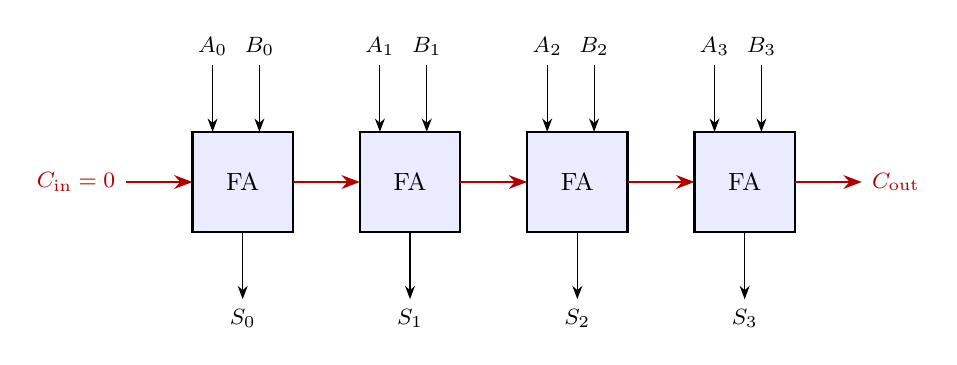
\begin{tikzpicture}[scale=0.85, >=Stealth]
  % 4 full adders
  \foreach \i/\x in {0/0, 1/2.5, 2/5, 3/7.5} {
    \draw[thick, fill=blue!8] (\x,0) rectangle (\x+1.5,1.5);
    \node[font=\small] at (\x+0.75,0.75) {FA};
  }
  % Inputs A and B
  \foreach \i/\x/\name in {0/0/A_0, 1/2.5/A_1, 2/5/A_2, 3/7.5/A_3} {
    \draw[->] (\x+0.3,2.5) node[above, font=\footnotesize]{$\name$} -- (\x+0.3,1.5);
    \draw[->] (\x+1.0,2.5) node[above, font=\footnotesize]{$B_\i$} -- (\x+1.0,1.5);
  }
  % Outputs S
  \foreach \i/\x in {0/0, 1/2.5, 2/5, 3/7.5} {
    \draw[->] (\x+0.75,0) -- (\x+0.75,-1) node[below, font=\footnotesize]{$S_\i$};
  }
  % Carry propagation
  \draw[->, thick, red!70!black] (-1,0.75) node[left, font=\footnotesize]{$C_{\text{in}}=0$} -- (0,0.75);
  \draw[->, thick, red!70!black] (1.5,0.75) -- (2.5,0.75);
  \draw[->, thick, red!70!black] (4,0.75) -- (5,0.75);
  \draw[->, thick, red!70!black] (6.5,0.75) -- (7.5,0.75);
  \draw[->, thick, red!70!black] (9,0.75) -- (10,0.75) node[right, font=\footnotesize]{$C_{\text{out}}$};
\end{tikzpicture}
\end{center}

\begin{formule}
\textbf{Délai du RCA :} la retenue doit ``traverser'' tous les étages. Si chaque additionneur complet a un délai $t_{FA}$ pour propager la retenue :
\[
\boxed{t_{\text{RCA},n} = n \cdot t_{FA}}
\]
Pour $n = 64$ bits avec $t_{FA} = \SI{50}{ps}$ : $t_{\text{RCA}} = \SI{3.2}{ns}$ $\Rightarrow$ $f_{\max} \approx \SI{310}{MHz}$. Insuffisant pour les processeurs modernes ($> \SI{3}{GHz}$).
\end{formule}

\begin{attention}
\textbf{Le ripple carry est le maillon faible.} La somme $S_i$ ne devient correcte qu'\textit{après} que la retenue $C_i$ soit arrivée depuis le bit $i-1$. C'est le \textbf{chemin critique} (chapitre 20) typique d'un processeur : la propagation de la retenue dans l'additionneur de l'ALU. Toutes les architectures arithmétiques avancées sont des tentatives de \textbf{briser cette dépendance séquentielle}.
\end{attention}

\subsection{Soustraction : un additionneur déguisé}

\begin{formule}
\textbf{Soustraction $A - B$ en complément à deux :}
\[
A - B = A + (-B) = A + \overline{B} + 1
\]
Réalisation : on inverse les bits de $B$ (XOR avec ``1'') et on injecte $C_{\text{in}} = 1$ dans le premier additionneur. Le même circuit additionneur réalise donc \textbf{addition et soustraction} avec une seule ligne de contrôle (XOR sur $B$, $C_{\text{in}}$). C'est l'élégance du complément à deux.
\end{formule}

\begin{retenir}
\textbf{L'essentiel :}
\begin{enumerate}[nosep]
\item Complément à deux : $-x = \overline{x} + 1$. Représentation universelle des entiers signés.
\item Ripple carry : simple, mais délai $\propto n$. Inutilisable au-delà de 8--16 bits à haute fréquence.
\item Soustraction = addition de l'opposé : le même additionneur fait les deux.
\item Toute l'arithmétique numérique tourne autour d'un problème : \textbf{propager la retenue plus vite}.
\end{enumerate}
\end{retenir}

% ============================================================================
\section{Approfondissement}

\vspace{0.3cm}
\textit{Comment briser la dépendance séquentielle de la retenue : les architectures rapides d'addition, et les structures de multiplication.}
\vspace{0.3cm}

\begin{approfondissement}
Carry lookahead, carry select, additionneurs préfixés, et structures de multiplication. Prérequis : chapitre 20 (logique combinatoire), section précédente.
\end{approfondissement}

\subsection{Carry lookahead : calculer la retenue à l'avance}

\begin{formule}
\textbf{Idée fondamentale :} au lieu d'attendre que la retenue arrive, on \textbf{calcule à l'avance} si chaque étage va générer ou propager une retenue.

Pour chaque bit $i$, on définit :
\begin{itemize}[nosep]
\item \textbf{Generate} : $G_i = A_i \cdot B_i$ (l'étage \textit{génère} une retenue si $A$ et $B$ sont tous deux à 1).
\item \textbf{Propagate} : $P_i = A_i \oplus B_i$ (l'étage \textit{propage} une retenue entrante si exactement un des deux est à 1).
\end{itemize}

La retenue $C_{i+1}$ s'exprime alors directement :
\[
C_{i+1} = G_i + P_i \cdot C_i
\]
En dépliant récursivement :
\[
C_1 = G_0 + P_0 C_0
\]
\[
C_2 = G_1 + P_1 G_0 + P_1 P_0 C_0
\]
\[
C_3 = G_2 + P_2 G_1 + P_2 P_1 G_0 + P_2 P_1 P_0 C_0
\]
\textbf{Toutes les retenues se calculent en parallèle} à partir des $G_i$, $P_i$ et $C_0$, en $\mathcal{O}(\log n)$ niveaux de portes au lieu de $\mathcal{O}(n)$.
\end{formule}

\begin{intuition}
\textbf{Le prix : la complexité combinatoire.} Pour $n$ bits, l'équation de $C_n$ contient $n+1$ termes avec des produits de jusqu'à $n$ variables. En pratique, on regroupe les bits par blocs (typiquement 4) avec un CLA local par bloc, puis on chaîne les blocs avec un second niveau de CLA. C'est le \textbf{carry lookahead hiérarchique}.
\end{intuition}

\subsection{Carry select : la course parallèle}

\begin{formule}
\textbf{Principe :} pour un bloc de bits, on calcule \textbf{en parallèle} deux versions de la somme : une en supposant $C_{\text{in}} = 0$, une en supposant $C_{\text{in}} = 1$. Quand la retenue réelle arrive, un multiplexeur sélectionne la bonne version.

\textbf{Avantage :} pas besoin d'attendre la retenue pour commencer le calcul.

\textbf{Coût :} double la logique d'addition par bloc (mais pas par bit : on partage la logique entre blocs).

\textbf{Délai :} $t_{\text{CSA}} \approx t_{\text{ripple,block}} + t_{\text{MUX}} \cdot (\text{nombre de blocs})$. Pour 64 bits en blocs de 8 : $t \approx 8 t_{FA} + 8 t_{\text{MUX}}$. Plus rapide que le RCA pur ($64 t_{FA}$) mais moins que le CLA.
\end{formule}

\subsection{Additionneurs préfixés : Kogge-Stone et Brent-Kung}

\begin{formule}
Les additionneurs modernes haute performance (utilisés dans tous les CPU haut de gamme) sont basés sur des structures de \textbf{calcul de préfixe parallèle} :

\begin{center}
\renewcommand{\arraystretch}{1.4}
\begin{tabular}{lccc}
\toprule
\textbf{Architecture} & \textbf{Profondeur} & \textbf{Surface (cellules)} & \textbf{Usage} \\
\midrule
Ripple Carry (RCA) & $n$ & $n$ & Microcontrôleurs simples \\
Carry Lookahead (CLA) & $\log_4 n$ & $\sim 2n$ & Standard FPGA/ASIC \\
Kogge-Stone & $\log_2 n$ & $n\log_2 n$ & CPU haute performance \\
Brent-Kung & $2\log_2 n - 1$ & $\sim 2n$ & Compromis vitesse/surface \\
Hybride Han-Carlson & $\log_2 n + 1$ & $\sim n\log_2 n / 2$ & ALU de processeurs modernes \\
\bottomrule
\end{tabular}
\end{center}
\end{formule}

\begin{intuition}
\textbf{L'intuition Kogge-Stone :} l'addition est un problème de \textit{préfixe parallèle} comme la somme cumulative. À chaque étage $k$, chaque bit combine son information avec celle du bit situé à $2^k$ positions en arrière. Après $\log_2 n$ étages, chaque bit a vu l'effet de tous les bits qui le précèdent.

Pour $n = 64$ : RCA fait 64 étages, Kogge-Stone n'en fait que 6. La différence est dramatique à haute fréquence.
\end{intuition}

\subsection{Multiplication : la somme de produits partiels}

\begin{formule}
La multiplication binaire suit le même principe que la multiplication décimale ``à la main'' :
\begin{itemize}[nosep]
\item Pour chaque bit $b_i$ de $B$, on calcule $A \times b_i$ (qui vaut $A$ si $b_i = 1$, $0$ sinon).
\item On décale ce produit partiel de $i$ positions vers la gauche.
\item On somme tous les produits partiels.
\end{itemize}

Pour $n$ bits, on a $n$ produits partiels à sommer.
\end{formule}

\begin{formule}
\textbf{Architectures de multiplication :}
\begin{itemize}[nosep]
\item \textbf{Multiplieur en réseau (\textit{array multiplier})} : grille régulière de cellules ET + additionneurs. Surface $\mathcal{O}(n^2)$, délai $\mathcal{O}(n)$. Simple mais lent.
\item \textbf{Multiplieur de Wallace} : arbre de réducteurs 3:2 (full adders utilisés comme compresseurs) qui réduit les $n$ produits partiels en 2 en $\mathcal{O}(\log_{3/2} n)$ étapes, puis un additionneur final. Délai $\mathcal{O}(\log n)$.
\item \textbf{Multiplieur de Dadda} : variante de Wallace optimisée pour utiliser moins de réducteurs. Surface réduite, même délai.
\item \textbf{Encodage de Booth} : réduit le nombre de produits partiels en regroupant les bits par 2 ou 3. Particulièrement efficace pour les multiplications signées.
\end{itemize}
\end{formule}

\begin{intuition}
\textbf{Pourquoi la multiplication est si gourmande :} un multiplieur 64$\times$64 bits contient typiquement $> 10\,000$ portes logiques et son chemin critique compte $\sim 20$--$30$ niveaux. C'est pourquoi les processeurs incluent des \textbf{multiplieurs dédiés} (souvent pipelinés sur 3--5 étages) plutôt que d'utiliser leur ALU pour multiplier. Les DSP et accélérateurs IA (TPU, GPU) ont des centaines à des milliers de multiplieurs en parallèle.
\end{intuition}

\subsection{Division : l'opération la plus coûteuse}

\begin{formule}
La division est intrinsèquement \textbf{séquentielle} : on ne peut pas calculer le chiffre suivant tant qu'on n'a pas terminé l'étape précédente.

\textbf{Algorithmes principaux :}
\begin{itemize}[nosep]
\item \textbf{Division par restauration} : 1 bit de quotient par cycle. Simple mais lent ($n$ cycles pour $n$ bits).
\item \textbf{SRT (Sweeney-Robertson-Tocher)} : 2--4 bits par cycle. Standard dans les FPU modernes (utilisé dans le Pentium FPU original, célèbre pour son bug de 1994).
\item \textbf{Newton-Raphson} : convergence quadratique vers $1/B$, puis multiplication. Très rapide mais nécessite une approximation initiale (typiquement par table).
\item \textbf{Goldschmidt} : multiplie successivement $A/B$ par des facteurs qui font tendre $B$ vers $1$.
\end{itemize}

\textbf{En pratique :} une division 64 bits prend typiquement 20 à 80 cycles d'horloge, soit $10$--$50\times$ plus qu'une multiplication. Les compilateurs cherchent activement à éviter les divisions (remplacement par multiplication par l'inverse précalculé, décalages, etc.).
\end{formule}

\subsection{Comparateurs}

\begin{formule}
\textbf{Comparateur $A = B$ :}
\[
\text{Equal} = \prod_{i=0}^{n-1} \overline{A_i \oplus B_i}
\]
$A$ et $B$ sont égaux ssi tous les XOR sont à 0. Délai $\mathcal{O}(\log n)$ par arbre de NAND.

\textbf{Comparateur $A < B$ :} se ramène à une soustraction $A - B$ et observation du bit de signe. Réutilise donc un additionneur.

\textbf{Comparateur magnitude (\textit{magnitude comparator}) :} compare bit à bit en partant du MSB. Dès qu'un bit diffère, le résultat est déterminé. Logique simple mais profondeur $\mathcal{O}(n)$ dans le pire cas (ou $\mathcal{O}(\log n)$ avec une structure préfixe).
\end{formule}

% ============================================================================
\section{Niveau Ingénieur}

\begin{ingenieur}
Le triangle des compromis surface/vitesse/puissance, l'arithmétique flottante (IEEE 754), et les unités spécialisées (DSP, GPU). Lien avec la physique CMOS et le timing.
\end{ingenieur}

\subsection{Le triangle des compromis}

\begin{formule}
Toute architecture arithmétique se situe sur un triangle vitesse--surface--puissance. On ne peut pas optimiser les trois simultanément :

\begin{center}
\renewcommand{\arraystretch}{1.4}
\begin{tabular}{p{3cm}p{2.5cm}p{2.5cm}p{4cm}}
\toprule
\textbf{Architecture} & \textbf{Vitesse} & \textbf{Surface} & \textbf{Quand l'utiliser} \\
\midrule
RCA & Lente & Minimale & MCU 8/16 bits, $f < \SI{100}{MHz}$ \\
CLA hiérarchique & Modérée & Modérée & Standard FPGA/ASIC, $f < \SI{1}{GHz}$ \\
Kogge-Stone & Maximale & Élevée & CPU haute performance, $f > \SI{2}{GHz}$ \\
Multiplieur Wallace pipeliné & Maximale & Très élevée & GPU, DSP, accélérateurs IA \\
\bottomrule
\end{tabular}
\end{center}
\end{formule}

\begin{intuition}
\textbf{Lien avec la consommation :} plus de surface = plus de transistors = plus de capacités à charger à chaque cycle = $P_{\text{dyn}} = \alpha C V_{DD}^2 f$ (chapitre 20) augmente. Un Kogge-Stone consomme plus d'énergie par addition qu'un RCA, mais permet une fréquence plus haute.

\textbf{Énergie par opération} (joules/add) : c'est la métrique pertinente pour les systèmes mobiles et l'IA. Kogge-Stone et RCA peuvent avoir une énergie par opération comparable si on adapte $V_{DD}$ à la fréquence visée (DVFS, \textit{Dynamic Voltage and Frequency Scaling}).
\end{intuition}

\subsection{L'arithmétique flottante : IEEE 754}

\begin{formule}
Un nombre flottant IEEE 754 est codé en trois champs :
\[
(-1)^{\text{signe}} \times 1{,}\text{mantisse} \times 2^{\text{exposant} - \text{biais}}
\]

\begin{center}
\renewcommand{\arraystretch}{1.3}
\begin{tabular}{lccccc}
\toprule
\textbf{Format} & \textbf{Total} & \textbf{Signe} & \textbf{Exposant} & \textbf{Mantisse} & \textbf{Précision} \\
\midrule
Simple (FP32) & 32 & 1 & 8 & 23 & $\sim 7$ chiffres décimaux \\
Double (FP64) & 64 & 1 & 11 & 52 & $\sim 15$ chiffres \\
Demi (FP16) & 16 & 1 & 5 & 10 & $\sim 3$ chiffres \\
bfloat16 & 16 & 1 & 8 & 7 & $\sim 2$ chiffres (large gamme) \\
\bottomrule
\end{tabular}
\end{center}

\textbf{Opérations flottantes :} addition et soustraction sont plus complexes que la multiplication ! Il faut :
\begin{enumerate}[nosep]
\item Aligner les exposants (décalage de la mantisse du plus petit).
\item Additionner ou soustraire les mantisses.
\item Renormaliser le résultat (ajuster exposant + décaler mantisse).
\item Arrondir.
\end{enumerate}
\end{formule}

\begin{attention}
\textbf{Pièges de l'arithmétique flottante :}
\begin{itemize}[nosep]
\item L'addition n'est \textbf{pas associative} : $(a+b)+c \neq a+(b+c)$ en général à cause des arrondis. Conséquence majeure : la parallélisation d'une somme peut donner un résultat \textit{différent} du calcul séquentiel.
\item \textbf{Cancellation catastrophique} : la soustraction de deux nombres proches perd la précision (les chiffres significatifs s'annulent).
\item \textbf{Dénormaux} : nombres très proches de zéro, traités avec une logique spéciale, plus lente.
\item L'IA moderne (deep learning) utilise massivement bfloat16 et même int8/int4 pour gagner en vitesse et en énergie au prix de la précision.
\end{itemize}
\end{attention}

\subsection{Unités spécialisées : MAC, DSP, tensor cores}

\begin{formule}
La multiplication-accumulation (MAC) est l'opération la plus fréquente en traitement du signal et en IA :
\[
\boxed{\text{acc} \leftarrow \text{acc} + a \times b}
\]

Pratiquement \textbf{tous} les processeurs modernes ont des unités MAC dédiées :
\begin{itemize}[nosep]
\item \textbf{DSP} : blocs MAC pipelinés ($\sim 5$ étages) capables de faire 1 MAC par cycle, soit $\SI{1}{GMAC/s}$ par bloc à $\SI{1}{GHz}$.
\item \textbf{GPU} : milliers d'unités MAC en parallèle (CUDA cores).
\item \textbf{Tensor cores (Nvidia) / TPU (Google)} : matrices systoliques de MAC qui calculent $C = A \times B + C$ (produit matriciel) en un seul ``cycle'' macroscopique.
\item \textbf{NPU dans les SoC mobiles} : MAC en int8/int4 pour l'inférence IA embarquée.
\end{itemize}
\end{formule}

\subsection{Conséquences sur le chemin critique}

\begin{formule}
Dans un processeur moderne, le chemin critique de l'ALU est souvent l'\textbf{additionneur 64 bits}. Sa profondeur $\log_2(64) = 6$ niveaux (Kogge-Stone) impose à elle seule $\sim\SI{200}{ps}$ de délai logique. C'est la \textbf{principale raison} qui limite la fréquence d'horloge à $\sim\SI{4}{GHz}$ dans les CPU généralistes (avec un peu de marge pour les autres chemins, le wire delay et le timing margin).

\textbf{Stratégies pour aller au-delà :}
\begin{itemize}[nosep]
\item \textbf{Pipeline de l'ALU} : découper l'addition en 2--3 étages (au prix de la latence).
\item \textbf{Opérations 32 bits préférées} : un additionneur 32 bits a $\log_2(32) = 5$ niveaux au lieu de 6.
\item \textbf{Out-of-order execution} : exécuter d'autres instructions pendant que l'addition se propage.
\end{itemize}
\end{formule}

% === EXERCICES ===
\section*{Exercices}
\addcontentsline{toc}{section}{Exercices}

\subsection*{Niveau débutant}

\textbf{Exercice 25.1 ---} Sur 8 bits en complément à deux, exprimez $-42$. Vérifiez en additionnant $42 + (-42)$.

\begin{pratique}
\textbf{Solution :} $42 = 00101010$. $\overline{42} = 11010101$. $+1 = 11010110 = -42$.

Vérification : $00101010 + 11010110 = 100000000$. On garde les 8 bits LSB : $00000000 = 0$. \checkmark
\end{pratique}

\textbf{Exercice 25.2 ---} Un microcontrôleur à $\SI{100}{MHz}$ utilise un additionneur ripple carry 16 bits avec $t_{FA} = \SI{200}{ps}$. L'addition tient-elle dans un cycle ?

\begin{pratique}
\textbf{Solution :} $T_{\text{clk}} = \SI{10}{ns}$. $t_{\text{RCA}} = 16\times200 = \SI{3.2}{ns}$. Budget restant pour setup, registres et autre logique : $10 - 3{,}2 = \SI{6.8}{ns}$. Largement suffisant pour 100 MHz. RCA reste pertinent ici.
\end{pratique}

\subsection*{Niveau intermédiaire}

\textbf{Exercice 25.3 ---} Un processeur à $\SI{3}{GHz}$ doit faire une addition 64 bits par cycle. Quel délai max pour l'additionneur ? Quelle architecture choisir entre RCA, CLA et Kogge-Stone ?

\begin{pratique}
\textbf{Solution :} $T_{\text{clk}} = \SI{333}{ps}$. En retirant $t_{cq}$, $t_{su}$, skew et marge ($\sim\SI{100}{ps}$), budget logique $\sim\SI{233}{ps}$.

RCA : $64 \times 50 = \SI{3.2}{ns}$. \textbf{Impossible} ($14\times$ trop lent).

CLA hiérarchique (16 blocs de 4) : $\sim\SI{500}{ps}$. Encore trop lent.

Kogge-Stone : $6$ niveaux $\times \sim\SI{30}{ps}$ = $\sim\SI{180}{ps}$. \textbf{OK}, avec marge.

Décision : \textbf{Kogge-Stone}, justifiée malgré sa surface accrue.
\end{pratique}

\textbf{Exercice 25.4 ---} Un multiplieur en réseau 8$\times$8 bits a un délai de $\sim 15 t_{FA}$. Comparez avec un Wallace 8$\times$8 ($\sim 6 t_{FA}$ pour la réduction + additionneur final 8 bits).

\begin{pratique}
\textbf{Solution :} Wallace : $6 t_{FA}$ (compression) + $\log_2(8) \times 2 t_{FA}$ (CLA 8 bits) $\approx 12 t_{FA}$.

Réseau : $15 t_{FA}$. Wallace est $\sim 20\%$ plus rapide. Pour des multiplieurs plus grands (32 bits, 64 bits), l'écart se creuse : Wallace gagne d'un facteur 2 à 3.
\end{pratique}

\subsection*{Niveau ingénieur}

\textbf{Exercice 25.5 ---} En FP32 (IEEE 754), calculez le résultat de $a + b + c$ avec $a = 10^{20}$, $b = -10^{20}$, $c = 1$. Que se passe-t-il selon l'ordre des opérations ?

\begin{pratique}
\textbf{Solution :}

Ordre $(a + b) + c$ : $a + b = 0$ exact. $0 + 1 = 1$. \checkmark

Ordre $a + (b + c)$ : $b + c = -10^{20} + 1$. Mais $10^{20}$ a un exposant binaire $\sim 67$, et la mantisse FP32 n'a que $24$ bits utiles (24 chiffres binaires). Le ``1'' est perdu dans l'arrondi : $b + c = -10^{20}$ exactement. Puis $a + (-10^{20}) = 0$.

\textbf{Résultat catastrophiquement différent !} $1$ vs $0$. C'est la cancellation catastrophique. La parallélisation d'une somme (qui change l'ordre) peut donner ce type de divergence numérique.
\end{pratique}

\textbf{Exercice 25.6 ---} Un GPU exécute $1024$ MAC FP32 par cycle à $\SI{1.5}{GHz}$.

(a) Combien d'opérations par seconde (FLOPS) ?

(b) Si chaque MAC consomme $\SI{30}{pJ}$ d'énergie, quelle puissance dissipée ?

(c) Pourquoi l'IA moderne préfère-t-elle bfloat16 ou int8 ?

\begin{pratique}
\textbf{Solution :}

(a) $1024 \times 1{,}5\times10^9 \times 2$ (un MAC = 1 mult + 1 add = 2 FLOP) $= 3{,}07\times10^{12}$ FLOPS = \SI{3.07}{TFLOPS}.

(b) $P = 1024 \times 30\times10^{-12} \times 1{,}5\times10^9 = \SI{46}{W}$. Ordre de grandeur d'un GPU mobile.

(c) bfloat16 / int8 : multiplieurs $\sim 4\times$ à $16\times$ plus petits (la complexité de la multiplication est $\propto n^2$). Plus de MAC par mm$^2$, moins d'énergie par opération. L'IA tolère cette précision réduite car les réseaux sont robustes au bruit numérique. Une carte qui fait \SI{300}{TFLOPS} en FP16 peut faire \SI{1.2}{TOPS} en int8.
\end{pratique}

\subsection*{Questions de compréhension}

\begin{enumerate}[nosep]
\item Pourquoi le complément à deux n'a-t-il qu'une seule représentation du zéro alors que le signe-magnitude en a deux (+0 et $-0$) ? Quel avantage matériel ?
\item Un additionneur Kogge-Stone a $n \log_2 n$ cellules contre $n$ pour le RCA. Pourquoi accepter ce coût en surface ?
\item L'addition flottante n'est pas associative à cause des arrondis. Pourquoi est-ce un problème majeur pour le calcul scientifique parallèle ?
\item Un compilateur remplace $x/8$ par $x \gg 3$ (décalage à droite de 3 bits). Pourquoi cette optimisation est-elle si importante ? Que se passe-t-il pour $x = -1$ en complément à deux ?
\end{enumerate}

% === RÉSUMÉ ===
\section*{Résumé du chapitre}
\addcontentsline{toc}{section}{Résumé du chapitre}

\begin{bases}[title={\color{white} Résumé --- Les Bases}]
\begin{center}
\renewcommand{\arraystretch}{1.3}
\begin{tabular}{p{3.5cm}p{9.5cm}}
\toprule
Complément à deux & $-x = \overline{x}+1$. Une seule représentation du zéro \\
RCA & Délai $= n \cdot t_{FA}$. Simple mais lent. Inutilisable $> \SI{16}{bits}$ à HF \\
Soustraction & $A - B = A + \overline{B} + 1$. Même circuit que l'addition \\
Enjeu central & Briser la dépendance séquentielle de la retenue \\
\bottomrule
\end{tabular}
\end{center}
\end{bases}

\begin{approfondissement}[title={\color{white} Résumé --- Approfondissement}]
\begin{center}
\renewcommand{\arraystretch}{1.3}
\begin{tabular}{p{3.5cm}p{9.5cm}}
\toprule
Carry lookahead & Generate/Propagate. Délai $\mathcal{O}(\log n)$ \\
Carry select & Calcul parallèle $C_{\text{in}}=0$ et $C_{\text{in}}=1$ + MUX \\
Kogge-Stone & Préfixe parallèle, $\log_2 n$ niveaux. Standard CPU haut de gamme \\
Multiplication & Réseau ($\mathcal{O}(n)$), Wallace ($\mathcal{O}(\log n)$), Booth (signé) \\
Division & Séquentielle. SRT, Newton-Raphson. $10$--$50\times$ plus lent que mult \\
\bottomrule
\end{tabular}
\end{center}
\end{approfondissement}

\begin{ingenieur}[title={\color{white} Résumé --- Niveau Ingénieur}]
\begin{center}
\renewcommand{\arraystretch}{1.3}
\begin{tabular}{p{3.5cm}p{9.5cm}}
\toprule
Triangle des compromis & Vitesse vs Surface vs Puissance. Pas d'optimum global \\
IEEE 754 & FP32, FP64, FP16, bfloat16. Pas associatif (arrondis) \\
Pièges flottants & Cancellation, dénormaux, ordre des opérations \\
Unités spécialisées & MAC (DSP), tensor cores, NPU. int8/int4 pour l'IA \\
ALU = chemin critique & Additionneur 64b limite $f_{\text{CPU}}$ à $\sim\SI{4}{GHz}$ \\
\bottomrule
\end{tabular}
\end{center}
\end{ingenieur}

% ============================================================================
% ============================================================================
% CHAPITRE 26 : ARCHITECTURE NUMÉRIQUE
% VERSION PEER-REVIEW
% Fichier autonome à intégrer dans Bible_Elec.tex
% ============================================================================

\chapter{Architecture numérique : du bloc au système}

\begin{center}
\textit{Nous avons maintenant toutes les briques : portes logiques,\\
bascules, FSM, additionneurs, mémoires.\\
Ce chapitre les assemble en un système qui calcule :\\
un chemin de données piloté par un contrôleur.\\
C'est le principe de tout processeur, DSP ou accélérateur ---\\
et c'est avant tout un problème de matériel, de timing et de physique.}
\end{center}

\vspace{0.5cm}

Les chapitres 20 à 25 ont construit les composants : logique combinatoire, bascules, machines d'état, mémoires, circuits arithmétiques. Ce chapitre montre comment les \textbf{assembler} en un système numérique complet. Le modèle universel est la séparation \textbf{datapath / contrôleur} : un chemin de données qui transporte et transforme les valeurs, et une FSM qui orchestre les opérations cycle par cycle. Nous resterons du côté \textit{matériel} : structures physiques, chemins critiques, compromis de conception --- pas un cours d'informatique.

% ============================================================================
\section{Les Bases}

\begin{bases}
La séparation datapath/contrôleur, les éléments du chemin de données, et un premier système complet. Prérequis : chapitres 21 (registres), 23 (FSM), 25 (ALU).
\end{bases}

\subsection{Le problème : orchestrer le calcul}

\begin{intuition}
\textbf{Un exemple concret :} calculer la somme des 100 premiers entiers. Il faut :
\begin{enumerate}[nosep]
\item Un registre \texttt{acc} pour l'accumulateur (initialisé à 0).
\item Un registre \texttt{i} pour le compteur (initialisé à 1).
\item Un additionneur pour \texttt{acc + i} et pour \texttt{i + 1}.
\item Un comparateur pour tester \texttt{i > 100}.
\item Quelque chose qui décide, à chaque cycle, \textit{quoi additionner, où ranger le résultat, et quand s'arrêter}.
\end{enumerate}
Les quatre premiers éléments forment le \textbf{datapath}. Le cinquième est le \textbf{contrôleur}. Cette séparation est le principe d'organisation de \textit{tout} système numérique de calcul.
\end{intuition}

\begin{formule}
\textbf{La séparation datapath / contrôleur :}

\begin{itemize}[nosep]
\item Le \textbf{datapath} (chemin de données) contient les éléments qui \textit{stockent} et \textit{transforment} les données : registres, ALU, multiplexeurs, bus, mémoires. Il est large ($n$ bits, typiquement 8 à 64).
\item Le \textbf{contrôleur} est une FSM (chapitre 23) qui génère les \textit{signaux de commande} : sélection des MUX, écriture des registres, opération de l'ALU. Il est étroit (quelques bits de contrôle) mais décide de tout.
\item Le datapath renvoie au contrôleur des \textbf{drapeaux} (\textit{flags}) : zéro, signe, retenue, comparaison --- les informations dont la FSM a besoin pour décider des transitions.
\end{itemize}
\end{formule}

\begin{center}
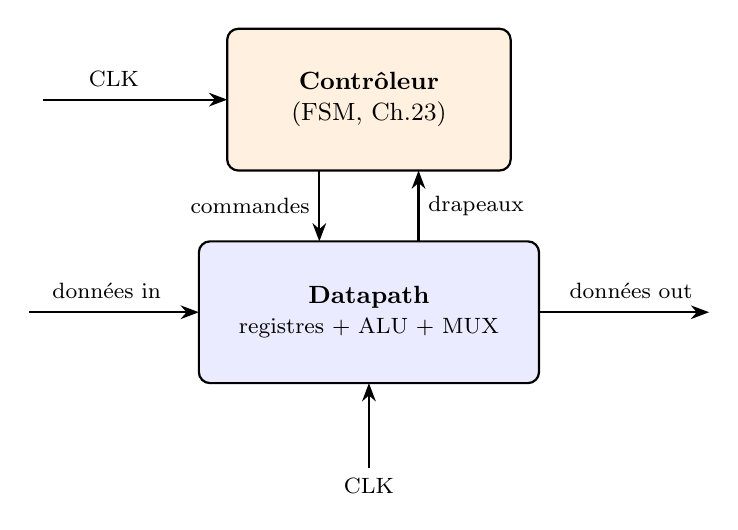
\begin{tikzpicture}[>=Stealth, scale=0.9]
  % Contrôleur
  \draw[thick, fill=orange!12, rounded corners=4pt] (0,3) rectangle (4,5);
  \node[font=\small, align=center] at (2,4) {\textbf{Contrôleur}\\(FSM, Ch.23)};
  % Datapath
  \draw[thick, fill=blue!8, rounded corners=4pt] (-0.4,0) rectangle (4.4,2);
  \node[font=\small, align=center] at (2,1) {\textbf{Datapath}\\{\footnotesize registres + ALU + MUX}};
  % Commandes
  \draw[->, thick] (1.3,3) -- (1.3,2);
  \node[font=\footnotesize, left] at (1.3,2.5) {commandes};
  % Flags
  \draw[->, thick] (2.7,2) -- (2.7,3);
  \node[font=\footnotesize, right] at (2.7,2.5) {drapeaux};
  % E/S données
  \draw[->, thick] (-2.8,1) -- (-0.4,1);
  \node[font=\footnotesize, above] at (-1.7,1.05) {données in};
  \draw[->, thick] (4.4,1) -- (6.8,1);
  \node[font=\footnotesize, above] at (5.7,1.05) {données out};
  % Horloge
  \draw[->, thick] (-2.6,4) -- (0,4);
  \node[font=\footnotesize, above] at (-1.6,4.05) {CLK};
  \draw[->, thick] (2,-1.2) -- (2,0);
  \node[font=\footnotesize, below] at (2,-1.2) {CLK};
\end{tikzpicture}
\end{center}

\subsection{Les éléments du datapath}

\begin{formule}
\textbf{Les quatre familles de blocs :}

\begin{center}
\renewcommand{\arraystretch}{1.4}
\begin{tabular}{p{2.8cm}p{4.5cm}p{5.5cm}}
\toprule
\textbf{Bloc} & \textbf{Fonction} & \textbf{Origine} \\
\midrule
\textbf{Registres} & Stocker les valeurs intermédiaires & Bascules D (Ch.21) \\
\textbf{ALU} & Add, sub, AND, OR, XOR, décalages, comparaisons & Circuits arithmétiques (Ch.25) \\
\textbf{Multiplexeurs} & Aiguiller les données vers les bonnes entrées & Logique combinatoire (Ch.20) \\
\textbf{Mémoire} & Stocker programmes et données en masse & SRAM/DRAM (Ch.24) \\
\bottomrule
\end{tabular}
\end{center}

Le datapath relie ces blocs par des \textbf{chemins de données} de largeur $n$ bits. À chaque cycle d'horloge, les données circulent : registre $\to$ MUX $\to$ ALU $\to$ MUX $\to$ registre.
\end{formule}

\begin{attention}
\textbf{Le cycle élémentaire du datapath} suit exactement le rythme de la logique séquentielle (chapitre 21) : \textbf{calcul combinatoire entre deux fronts, capture au front}. Au front d'horloge, les registres capturent. Pendant le cycle, les données traversent MUX et ALU. Au front suivant, le résultat est capturé. La fréquence maximale est donnée par le chemin le plus lent du datapath :
\[
T_{\text{clk}} \geq t_{cq} + t_{\text{MUX}} + t_{\text{ALU}} + t_{\text{MUX}} + t_{su}
\]
L'ALU (et en particulier son additionneur, chapitre 25) domine généralement ce chemin.
\end{attention}

\subsection{L'ALU : le cœur transformateur}

\begin{formule}
L'\textbf{ALU} (\textit{Arithmetic and Logic Unit}) regroupe les opérations de base derrière un sélecteur :

\begin{itemize}[nosep]
\item Un additionneur/soustracteur (chapitre 25 : même circuit, signal de contrôle \texttt{sub}).
\item Des opérations logiques bit à bit : AND, OR, XOR, NOT.
\item Des décalages : logiques ($\ll$, $\gg$), arithmétiques (préservent le signe), rotations.
\item Un \textbf{MUX final} qui sélectionne le résultat selon le code d'opération (\textit{opcode}).
\end{itemize}

L'ALU produit aussi les \textbf{drapeaux} :
\begin{itemize}[nosep]
\item \texttt{Z} (zéro) : le résultat est nul. Réalisé par un grand NOR de tous les bits.
\item \texttt{N} (négatif) : le MSB du résultat (complément à deux).
\item \texttt{C} (carry) : la retenue sortante de l'additionneur.
\item \texttt{V} (overflow) : débordement signé, $V = C_{n} \oplus C_{n-1}$ (les deux dernières retenues diffèrent).
\end{itemize}
\end{formule}

\begin{retenir}
\textbf{L'essentiel :}
\begin{enumerate}[nosep]
\item Tout système de calcul = \textbf{datapath} (large, transforme les données) + \textbf{contrôleur} (FSM, décide).
\item Le datapath = registres + ALU + MUX + mémoire, reliés par des chemins de $n$ bits.
\item Le contrôleur envoie des commandes, le datapath renvoie des drapeaux.
\item La fréquence est limitée par le chemin le plus lent du datapath (souvent l'ALU).
\end{enumerate}
\end{retenir}

% ============================================================================
\section{Approfondissement}

\vspace{0.3cm}
\textit{Les structures qui font un vrai processeur : le banc de registres multi-ports, les bus, et l'assemblage complet fetch-decode-execute.}
\vspace{0.3cm}

\begin{approfondissement}
Banc de registres, architectures de bus, et construction d'un mini-processeur. Prérequis : sections précédentes, chapitre 24 (SRAM).
\end{approfondissement}

\subsection{Le banc de registres (register file)}

\begin{formule}
Le \textbf{banc de registres} est un petit tableau de registres adressables ($16$ à $64$ registres de $n$ bits), avec plusieurs \textbf{ports} d'accès simultanés :

\begin{itemize}[nosep]
\item \textbf{2 ports de lecture} : pour lire les deux opérandes d'une instruction (\texttt{a + b}) \textit{dans le même cycle}.
\item \textbf{1 port d'écriture} : pour ranger le résultat.
\end{itemize}

\textbf{Structure interne :} une matrice de cellules (bascules D ou cellules SRAM, chapitre 24) avec :
\begin{itemize}[nosep]
\item Un \textbf{décodeur d'adresse} par port (chapitre 20) qui active la ligne du registre visé.
\item Pour la lecture : des multiplexeurs larges (ou des lignes de bit partagées avec sense amplifiers, comme une SRAM).
\item Pour l'écriture : un signal \texttt{write enable} validé au front d'horloge.
\end{itemize}
\end{formule}

\begin{attention}
\textbf{Le coût physique des ports.} Chaque port supplémentaire ajoute un décodeur, des lignes de mot, et des transistors d'accès \textit{à chaque cellule}. La surface du banc de registres croît environ en $\mathcal{O}(p^2)$ avec le nombre de ports $p$ (les lignes horizontales et verticales se multiplient). Un banc 16 registres $\times$ 64 bits avec 2R+1W est raisonnable ; un banc avec 8 ports de lecture (processeurs superscalaires larges) devient un bloc dominant en surface et en énergie. C'est une contrainte physique majeure de l'architecture des processeurs.
\end{attention}

\subsection{Les bus : partager les chemins de données}

\begin{formule}
Quand plusieurs blocs doivent échanger des données, deux approches :

\textbf{1. Bus partagé à trois états (tristate)} : tous les blocs se connectent au même fil. Un seul émetteur actif à la fois (les autres sorties sont en haute impédance, \textit{Hi-Z}).
\begin{itemize}[nosep]
\item Avantage : peu de fils.
\item Inconvénients : risque de \textbf{conflit de bus} (deux émetteurs actifs $\Rightarrow$ court-circuit $V_{DD}$--GND à travers les étages de sortie), capacité de bus élevée (tous les récepteurs se cumulent) $\Rightarrow$ lent, difficile à tester.
\end{itemize}

\textbf{2. Multiplexage (MUX-based)} : chaque destination a un MUX qui sélectionne sa source.
\begin{itemize}[nosep]
\item Avantages : pas de conflit possible, chemins point à point rapides, analyse de timing simple (STA, chapitre 22).
\item Inconvénient : plus de fils et de logique.
\end{itemize}

\textbf{En pratique :} les conceptions sur puce modernes utilisent quasi exclusivement le \textbf{multiplexage}. Le tristate survit sur les bus de carte (PCB) où le nombre de fils compte (bus mémoire externes, anciens bus PCI).
\end{formule}

\subsection{Construire un mini-processeur}

\begin{formule}
\textbf{Le cycle fetch-decode-execute, vu côté matériel :}

Un processeur exécute des instructions stockées en mémoire. Chaque instruction traverse trois phases, orchestrées par le contrôleur :

\begin{enumerate}[nosep]
\item \textbf{Fetch} : le registre \textbf{PC} (\textit{Program Counter}) adresse la mémoire d'instructions ; l'instruction lue est capturée dans le registre d'instruction \textbf{IR}. En parallèle, $\text{PC} \leftarrow \text{PC} + 4$ (incrément par l'additionneur).
\item \textbf{Decode} : les champs de l'IR sont extraits : opcode (vers le contrôleur), numéros de registres sources/destination (vers le banc de registres), constante immédiate (vers une extension de signe).
\item \textbf{Execute} : l'ALU opère sur les opérandes lus ; le résultat est écrit dans le banc de registres ou utilisé comme adresse mémoire (load/store) ; les branchements modifient le PC selon les drapeaux.
\end{enumerate}
\end{formule}

\begin{formule}
\textbf{Deux organisations temporelles :}

\textbf{Mono-cycle} : toute l'instruction (fetch + decode + execute + écriture) tient dans \textit{un seul} cycle d'horloge. Le chemin critique traverse \textit{tout} : mémoire d'instructions $\to$ banc de registres $\to$ ALU $\to$ mémoire de données $\to$ banc de registres.
\[
T_{\text{clk}} \geq t_{\text{mem,I}} + t_{\text{RF,read}} + t_{\text{ALU}} + t_{\text{mem,D}} + t_{\text{RF,write}}
\]
Simple à concevoir, mais le cycle est dimensionné par l'instruction \textit{la plus lente} (load), même si la plupart des instructions sont plus rapides. Fréquence faible.

\textbf{Multi-cycle} : chaque phase prend un cycle (3 à 5 cycles par instruction). Le contrôleur est une FSM qui séquence les phases. Le chemin critique par cycle est plus court $\Rightarrow$ fréquence plus haute, et les ressources (un seul additionneur, une seule mémoire) sont réutilisées entre les phases. Le débit reste de $\sim 1$ instruction tous les 3--5 cycles.
\end{formule}

\begin{intuition}
\textbf{Le contrôleur du multi-cycle est exactement une FSM du chapitre 23 :} ses états sont les phases (FETCH, DECODE, EXEC, MEM, WB), ses entrées sont l'opcode et les drapeaux, ses sorties sont les dizaines de signaux de commande du datapath. La conception suit la méthodologie du chapitre 23 : diagramme d'états $\to$ codage $\to$ logique de transition. Un processeur n'a rien de magique : c'est un datapath + une grosse FSM.
\end{intuition}

\subsection{Les jeux d'instructions : RISC vs CISC, ARM vs RISC-V}

Le \textbf{jeu d'instructions} (ISA, \textit{Instruction Set Architecture}) est le contrat entre matériel et logiciel : la liste des opérations que le décodeur sait traduire en signaux de commande. Ce choix n'est pas qu'informatique --- il a des conséquences \textbf{physiques directes} sur la surface du décodeur, la profondeur du pipeline et l'énergie par instruction.

\begin{formule}
\textbf{Les deux philosophies historiques :}

\begin{center}
\renewcommand{\arraystretch}{1.45}
\begin{tabular}{p{3.2cm}p{4.7cm}p{4.7cm}}
\toprule
\textbf{Critère} & \textbf{CISC} (x86, 68000) & \textbf{RISC} (ARM, RISC-V, MIPS) \\
\midrule
Philosophie & Instructions riches, proches du langage haut niveau & Instructions simples et régulières \\
Nombre d'instructions & Centaines à milliers (x86 : $>1500$) & Quelques dizaines (jeu de base) \\
Longueur d'instruction & \textbf{Variable} (1 à 15 octets en x86) & \textbf{Fixe} (32 bits, ou 16/32 compressé) \\
Accès mémoire & Dans presque toute instruction & \textbf{Load/store uniquement} \\
Registres généraux & Peu (x86 historique : 8) & Beaucoup (32 typique) \\
Décodeur (silicium) & \textbf{Très complexe} : microcode, plusieurs étages de pipeline & \textbf{Compact} : décodage direct, 1 niveau de logique \\
Cycles par instruction & Variable (1 à $>100$) & $\sim 1$ (avec pipeline) \\
\bottomrule
\end{tabular}
\end{center}
\end{formule}

\begin{intuition}
\textbf{Pourquoi le RISC a gagné --- physiquement :} une instruction de longueur fixe se décode avec une simple tranche de logique combinatoire : les champs sont toujours aux mêmes positions, donc câblés directement vers le banc de registres et l'ALU. Une instruction x86 de longueur variable exige d'abord de \textit{trouver où elle se termine} --- un problème séquentiel coûteux en portes et en étages de pipeline. Les x86 modernes ont tranché : leur décodeur \textbf{traduit le CISC en micro-opérations internes de type RISC}. Le cœur d'exécution d'un x86 actuel \textit{est} un RISC ; le CISC ne survit qu'à l'interface, pour la compatibilité logicielle --- au prix d'un décodeur qui consomme une fraction notable de la surface et de l'énergie du front-end.
\end{intuition}

\begin{attention}
\textbf{Précision importante : ARM \textit{est} une architecture RISC.} La comparaison pertinente aujourd'hui n'est donc pas ``RISC ou ARM'', mais \textbf{ARM ou RISC-V} : deux ISA de la même famille RISC, qui diffèrent par leur modèle d'ouverture et de licence --- avec des conséquences très concrètes pour le concepteur de circuits.
\end{attention}

\begin{formule}
\textbf{ARM vs RISC-V : le choix du concepteur de SoC :}

\begin{center}
\renewcommand{\arraystretch}{1.45}
\begin{tabular}{p{3.0cm}p{4.8cm}p{4.8cm}}
\toprule
\textbf{Critère} & \textbf{ARM} & \textbf{RISC-V} \\
\midrule
Modèle & ISA \textbf{propriétaire} (ARM Ltd) & ISA \textbf{libre et ouverte} (RISC-V International) \\
Coût pour l'ASIC & Licence + \textbf{royalties par puce} vendue & ISA gratuite (cœurs commerciaux payants possibles : SiFive, Andes\ldots) \\
Écosystème & Très mature : 30+ ans d'outils, debug, OS, middleware & Jeune, croissance rapide ; GCC/LLVM matures \\
Modularité & Profils fixés par ARM (Cortex-M/R/A) & \textbf{Modulaire} : base RV32I/RV64I + extensions M, A, F, D, C, V\ldots \\
Instructions custom & Interdites (sauf licence architecturale, rare et chère) & \textbf{Autorisées} : on peut greffer ses propres instructions (accélérateurs dédiés) \\
Vérification & Cœurs livrés \textbf{pré-vérifiés} par ARM & À la charge de l'intégrateur si cœur libre \\
Exemples & Cortex-M4 (nRF52, STM32), Cortex-A (smartphones), Neoverse (serveurs) & ESP32-C3, contrôleurs SSD Western Digital, cœurs SiFive \\
Cas d'usage type & Produit industriel, time-to-market court, écosystème logiciel requis & Très gros volumes (économie de royalties), instructions spécialisées, recherche \\
\bottomrule
\end{tabular}
\end{center}
\end{formule}

\begin{intuition}
\textbf{Le critère de décision :} à architecture comparable (Cortex-M4 vs cœur RV32IMC), performances et surface silicium sont du même ordre --- l'ISA RISC est ce qu'elle est. La différence se joue sur trois axes : le \textbf{coût} (les royalties ARM pèsent sur les très gros volumes), l'\textbf{écosystème} (ARM domine largement en outillage et bibliothèques éprouvées), et la \textbf{personnalisation} (RISC-V permet d'intégrer une instruction custom --- par exemple un MAC spécialisé du chapitre 25 --- directement dans le pipeline, ce qu'ARM interdit). Pour un nœud IoT industriel : ARM Cortex-M reste le choix de sécurité. Pour un accélérateur dédié à très fort volume : RISC-V devient très attractif.
\end{intuition}

% ============================================================================
\section{Niveau Ingénieur}

\begin{ingenieur}
Le pipeline matériel, ses aléas, le forwarding, et les limites physiques du datapath. Lien direct avec le timing (Ch.22) et l'arithmétique (Ch.25).
\end{ingenieur}

\subsection{Le pipeline : superposer les instructions}

\begin{formule}
Le \textbf{pipeline} applique au processeur l'idée du chapitre 21 (pipeline = découper le chemin critique) : on insère des \textbf{registres de pipeline} entre les phases, et chaque phase traite \textit{une instruction différente} simultanément :

\begin{center}
\renewcommand{\arraystretch}{1.3}
\begin{tabular}{l|ccccc}
\toprule
\textbf{Cycle} & 1 & 2 & 3 & 4 & 5 \\
\midrule
Instruction 1 & F & D & E & M & W \\
Instruction 2 & & F & D & E & M \\
Instruction 3 & & & F & D & E \\
\bottomrule
\end{tabular}
\end{center}

\textbf{Résultat :} en régime établi, \textbf{1 instruction terminée par cycle} (débit), alors que chaque instruction prend toujours 5 cycles (latence). La fréquence est fixée par l'étage le plus lent :
\[
T_{\text{clk}} \geq \max_k(t_{\text{étage},k}) + t_{cq} + t_{su}
\]
L'équilibrage des étages est crucial : un étage 2$\times$ plus lent que les autres gaspille la moitié du potentiel.
\end{formule}

\subsection{Les aléas : quand le pipeline se contredit}

\begin{attention}
Le pipeline superpose des instructions qui, logiquement, devraient s'exécuter l'une après l'autre. Trois familles de conflits (\textit{hazards}) apparaissent :

\textbf{1. Aléa de données} : l'instruction 2 a besoin du résultat de l'instruction 1, qui n'est pas encore écrit dans le banc de registres.

\textbf{2. Aléa de contrôle} : un branchement change le PC, mais les instructions suivantes sont déjà entrées dans le pipeline (elles doivent être annulées : \textit{flush}).

\textbf{3. Aléa structurel} : deux instructions veulent la même ressource au même cycle (ex : une seule mémoire pour instructions et données).
\end{attention}

\begin{formule}
\textbf{Le forwarding (bypass) : la solution matérielle à l'aléa de données.}

Plutôt que d'attendre que le résultat soit écrit puis relu dans le banc de registres, on ajoute des \textbf{chemins de contournement} : la sortie de l'ALU (étage E) est renvoyée \textit{directement} à l'entrée de l'ALU pour l'instruction suivante, via un MUX supplémentaire.

\textbf{Coût matériel :} des MUX larges ($n$ bits) sur les deux entrées de l'ALU, et une \textbf{logique de détection} (comparateurs d'adresses de registres entre étages). Ces MUX s'ajoutent au chemin critique de l'étage Execute :
\[
t_{\text{E}} = t_{\text{MUX,fwd}} + t_{\text{ALU}} + t_{\text{MUX,fwd}}
\]
Le forwarding accélère le programme (pas de cycle d'attente) mais ralentit légèrement l'horloge. Le bilan est très favorable --- tous les processeurs pipelinés l'utilisent.
\end{formule}

\subsection{Le chemin critique du datapath pipeliné}

\begin{formule}
Dans un processeur 5 étages typique, les candidats au chemin critique sont :

\begin{center}
\renewcommand{\arraystretch}{1.3}
\begin{tabular}{p{2.5cm}p{6cm}p{4.5cm}}
\toprule
\textbf{Étage} & \textbf{Chemin} & \textbf{Dominé par} \\
\midrule
Fetch & Lecture mémoire d'instructions & SRAM cache (Ch.24) \\
Decode & Lecture banc de registres + décodage & Décodeur + MUX de lecture \\
Execute & MUX fwd + ALU + MUX fwd & \textbf{Additionneur 64 bits (Ch.25)} \\
Memory & Accès cache de données & SRAM + comparaison de tags \\
Writeback & Écriture banc de registres & Court \\
\bottomrule
\end{tabular}
\end{center}

En pratique, \textbf{Execute} (l'additionneur + forwarding) et \textbf{Memory} (le cache) se disputent le chemin critique. C'est pourquoi les processeurs haute fréquence utilisent des additionneurs préfixés (Kogge-Stone, chapitre 25) et des caches pipelinés sur 2 cycles.
\end{formule}

\subsection{Limites physiques et consommation}

\begin{formule}
\textbf{Trois murs physiques de l'architecture :}

\textbf{1. Le banc de registres multi-ports} : la surface croît en $\mathcal{O}(p^2)$ avec le nombre de ports. Les architectures superscalaires (4--8 instructions/cycle) le contournent en \textit{dupliquant} le banc (copies synchronisées) ou en le partitionnant (clusters).

\textbf{2. La distribution des signaux de contrôle} : le contrôleur pilote des dizaines de signaux qui doivent traverser tout le datapath. À haute fréquence, le \textbf{wire delay} (chapitre 22) de ces signaux devient comparable au cycle $\Rightarrow$ on pipeline aussi le contrôle.

\textbf{3. L'énergie du mouvement de données} : déplacer un mot de 64 bits sur \SI{1}{mm} de fil coûte plus d'énergie que l'additionner. Conséquence architecturale majeure : rapprocher mémoire et calcul (caches hiérarchiques, \textit{near-memory computing}, architectures systoliques des accélérateurs IA). L'énergie, pas la logique, dicte l'architecture moderne.
\end{formule}

\begin{intuition}
\textbf{Ordres de grandeur (techno $\sim\SI{7}{nm}$, valeurs indicatives) :}
\begin{itemize}[nosep]
\item Addition 64 bits : $\sim\SI{0.1}{pJ}$.
\item Lecture banc de registres : $\sim\SI{0.3}{pJ}$.
\item Lecture cache L1 (SRAM, \SI{32}{ko}) : $\sim\SI{1}{pJ}$.
\item Accès DRAM externe : $\sim\SI{100}{pJ}$--$\SI{1000}{pJ}$ --- \textbf{1000 à 10\,000 fois l'addition}.
\end{itemize}
La hiérarchie mémoire (Ch.24) n'est pas qu'une question de latence : c'est d'abord une question d'\textbf{énergie}.
\end{intuition}

% === EXERCICES ===
\section*{Exercices}
\addcontentsline{toc}{section}{Exercices}

\subsection*{Niveau débutant}

\textbf{Exercice 26.1 ---} Pour le système ``somme des 100 premiers entiers'' de l'introduction, listez les signaux de commande que le contrôleur doit générer et les drapeaux qu'il doit recevoir.

\begin{pratique}
\textbf{Solution :} Commandes : \texttt{load\_acc} (écriture du registre acc), \texttt{load\_i}, \texttt{sel\_op} (MUX : l'ALU calcule acc+i ou i+1), \texttt{init} (charger 0 et 1 au départ). Drapeau : \texttt{i\_gt\_100} (sortie du comparateur $i > 100$). La FSM a 3 états : INIT, LOOP (additionner et incrémenter), DONE.
\end{pratique}

\textbf{Exercice 26.2 ---} Une ALU 32 bits produit le drapeau Z (zéro). Proposez sa réalisation logique et estimez sa profondeur en portes NOR/NAND à 4 entrées.

\begin{pratique}
\textbf{Solution :} $Z = 1$ ssi les 32 bits sont nuls : $Z = \overline{b_{31} + b_{30} + \cdots + b_0}$. Avec des NOR à 4 entrées en arbre : $32 \to 8 \to 2 \to 1$, soit $\lceil\log_4 32\rceil = 3$ niveaux (avec ajustement NAND/NOR pour les polarités). Profondeur $\sim 3$ portes : le drapeau Z est rapide, il ne domine pas le chemin critique.
\end{pratique}

\subsection*{Niveau intermédiaire}

\textbf{Exercice 26.3 ---} Un processeur mono-cycle a : $t_{\text{mem,I}} = \SI{2}{ns}$, $t_{\text{RF,read}} = \SI{0.8}{ns}$, $t_{\text{ALU}} = \SI{1.5}{ns}$, $t_{\text{mem,D}} = \SI{2}{ns}$, $t_{\text{RF,write}} = \SI{0.5}{ns}$.

(a) Quelle est la fréquence maximale ?

(b) En multi-cycle (chaque phase = 1 cycle, le cycle est fixé par la phase la plus lente), quelle fréquence et quel temps par instruction (5 phases) ?

\begin{pratique}
\textbf{Solution :}

(a) $T = 2+0{,}8+1{,}5+2+0{,}5 = \SI{6.8}{ns}$ $\Rightarrow$ $f_{\max} = \SI{147}{MHz}$. Chaque instruction : \SI{6.8}{ns}.

(b) Phase la plus lente : \SI{2}{ns} (mémoires) $\Rightarrow$ $f_{\max} = \SI{500}{MHz}$. Une instruction de 5 phases : $5\times2 = \SI{10}{ns}$. \textbf{Plus lent par instruction} que le mono-cycle ! Le multi-cycle ne gagne que si les instructions courtes (3--4 phases) dominent, ou comme étape vers le pipeline.
\end{pratique}

\textbf{Exercice 26.4 ---} Le même processeur est pipeliné en 5 étages avec registres de pipeline ($t_{cq} = \SI{0.1}{ns}$, $t_{su} = \SI{0.1}{ns}$).

(a) Quelle fréquence maximale ?

(b) Quel débit en régime établi, et quel gain par rapport au mono-cycle ?

\begin{pratique}
\textbf{Solution :}

(a) Étage le plus lent : \SI{2}{ns} (mémoire). $T_{\text{clk}} = 2 + 0{,}1 + 0{,}1 = \SI{2.2}{ns}$ $\Rightarrow$ $f_{\max} = \SI{455}{MHz}$.

(b) Débit : 1 instruction/cycle = \SI{455}{Minstr/s}. Mono-cycle : $1/6{,}8\,\text{ns} = \SI{147}{Minstr/s}$. \textbf{Gain $\times 3{,}1$} (et non $\times 5$ : les étages ne sont pas équilibrés, et les registres de pipeline coûtent $\SI{0.2}{ns}$/cycle).
\end{pratique}

\subsection*{Niveau ingénieur}

\textbf{Exercice 26.5 ---} Dans le pipeline de l'exercice 26.4, l'instruction \texttt{add r3, r1, r2} est immédiatement suivie de \texttt{sub r5, r3, r4} (qui lit r3).

(a) Sans forwarding, combien de cycles d'attente (bulles) faut-il insérer ? (L'écriture du banc se fait en W, la lecture en D ; on suppose l'écriture en première demi-période et la lecture en seconde.)

(b) Avec forwarding E$\to$E, combien de bulles ?

(c) Le forwarding ajoute $2\times t_{\text{MUX}} = \SI{0.2}{ns}$ à l'étage E ($t_E$ passe de \SI{1.5}{ns} à \SI{1.7}{ns}). La fréquence change-t-elle ?

\begin{pratique}
\textbf{Solution :}

(a) \texttt{add} écrit r3 en W (cycle 5). \texttt{sub} lit r3 en D (cycle 3). Avec écriture/lecture en demi-périodes opposées, \texttt{sub} peut lire au cycle 5 $\Rightarrow$ il faut retarder D de 2 cycles : \textbf{2 bulles}.

(b) Le résultat de \texttt{add} sort de E au cycle 3 ; \texttt{sub} en a besoin en E au cycle 4. Le forwarding E$\to$E fournit la valeur juste à temps : \textbf{0 bulle}.

(c) L'étage le plus lent reste la mémoire (\SI{2}{ns} $>$ \SI{1.7}{ns}) : la fréquence ne change pas. Le forwarding est ici ``gratuit'' en fréquence --- c'est le cas favorable typique.
\end{pratique}

\textbf{Exercice 26.6 ---} Un banc de registres 32$\times$64 bits doit passer de 2R+1W à 6R+3W pour un cœur superscalaire.

(a) En supposant une surface $\propto (\text{lignes de mot})\times(\text{lignes de bit})$, c'est-à-dire $\propto p^2$ avec $p$ le nombre total de ports, estimez le facteur d'augmentation de surface.

(b) Citez deux techniques pour limiter ce coût.

\begin{pratique}
\textbf{Solution :}

(a) $p$ passe de 3 à 9 : surface $\times (9/3)^2 = \times 9$. Le banc devient un bloc dominant.

(b) \textbf{Duplication} : deux copies 3R+3W écrites en parallèle (surface $\times 2$ au lieu de $\times 9$ pour les lectures, au prix de la cohérence des écritures). \textbf{Partitionnement (clustering)} : deux clusters de calcul avec chacun un banc local 3R+2W, et un réseau d'échange inter-clusters (coût : latence d'un cycle pour les communications croisées).
\end{pratique}

\subsection*{Questions de compréhension}

\begin{enumerate}[nosep]
\item Pourquoi sépare-t-on systématiquement datapath et contrôleur, plutôt que de concevoir un bloc unique ? Donnez un argument de conception et un argument de vérification.
\item Pourquoi les bus tristate ont-ils disparu des conceptions sur puce au profit des MUX ? Citez le risque électrique et le problème d'analyse de timing.
\item Le pipeline multiplie le débit mais pas la latence. Pourquoi les branchements (aléas de contrôle) sont-ils d'autant plus coûteux que le pipeline est profond ?
\item Déplacer une donnée depuis la DRAM coûte $\sim 1000\times$ l'énergie d'une addition. Quelle conséquence architecturale directe pour les accélérateurs d'IA ?
\end{enumerate}

% === RÉSUMÉ ===
\section*{Résumé du chapitre}
\addcontentsline{toc}{section}{Résumé du chapitre}

\begin{bases}[title={\color{white} Résumé --- Les Bases}]
\begin{center}
\renewcommand{\arraystretch}{1.3}
\begin{tabular}{p{3.5cm}p{9.5cm}}
\toprule
Datapath / contrôleur & Datapath = registres + ALU + MUX (large). Contrôleur = FSM (Ch.23) \\
Dialogue & Contrôleur $\to$ commandes ; datapath $\to$ drapeaux (Z, N, C, V) \\
ALU & Add/sub + logique + décalages derrière un MUX d'opcode \\
Timing & $T_{\text{clk}} \geq t_{cq} + t_{\text{MUX}} + t_{\text{ALU}} + t_{\text{MUX}} + t_{su}$ \\
\bottomrule
\end{tabular}
\end{center}
\end{bases}

\begin{approfondissement}[title={\color{white} Résumé --- Approfondissement}]
\begin{center}
\renewcommand{\arraystretch}{1.3}
\begin{tabular}{p{3.5cm}p{9.5cm}}
\toprule
Banc de registres & 2R+1W typique. Surface $\propto p^2$ : les ports coûtent cher \\
Bus & Tristate (conflits, capacité) abandonné sur puce $\to$ MUX partout \\
Mini-processeur & Fetch (PC, IR) $\to$ Decode $\to$ Execute. Contrôleur = FSM \\
Mono vs multi-cycle & Mono : cycle dimensionné par l'instruction la plus lente. Multi : FSM de phases \\
\bottomrule
\end{tabular}
\end{center}
\end{approfondissement}

\begin{ingenieur}[title={\color{white} Résumé --- Niveau Ingénieur}]
\begin{center}
\renewcommand{\arraystretch}{1.3}
\begin{tabular}{p{3.5cm}p{9.5cm}}
\toprule
Pipeline & Débit 1 instr/cycle ; $T_{\text{clk}} = \max(t_{\text{étage}}) + t_{cq} + t_{su}$. Équilibrage crucial \\
Aléas & Données (forwarding), contrôle (flush), structurels (dupliquer) \\
Forwarding & MUX de bypass autour de l'ALU : supprime les bulles, allonge un peu l'étage E \\
Chemin critique & Execute (additionneur, Ch.25) vs Memory (cache SRAM, Ch.24) \\
Énergie & DRAM $\sim 1000\times$ l'addition : l'énergie du mouvement de données dicte l'architecture \\
\bottomrule
\end{tabular}
\end{center}
\end{ingenieur}

% ============================================================================
% ============================================================================
% CHAPITRE 27 : CONVERSION ANALOGIQUE-NUMÉRIQUE ET NUMÉRIQUE-ANALOGIQUE
% VERSION PEER-REVIEW
% Fichier autonome à intégrer dans Bible_Elec.tex
% ============================================================================

\chapter{Conversion analogique-numérique et numérique-analogique}

\begin{center}
\textit{Le monde physique est analogique ; le traitement est numérique.\\
Entre les deux, deux circuits font le pont : l'ADC qui échantillonne\\
et quantifie, le DAC qui reconstruit. Ce pont n'est pas parfait :\\
chaque conversion perd de l'information, ajoute du bruit,\\
et déforme le signal. Concevoir une chaîne de conversion,\\
c'est choisir précisément ce qu'on accepte de perdre.}
\end{center}

\vspace{0.5cm}

Toute la partie numérique (chapitres 20--26) suppose que les données existent déjà sous forme de bits. Mais un capteur de température, un microphone, une antenne délivrent des \textbf{tensions continues}. Ce chapitre traite la frontière : comment transformer une tension en nombre (\textbf{ADC}, \textit{Analog-to-Digital Converter}) et un nombre en tension (\textbf{DAC}, \textit{Digital-to-Analog Converter}). C'est le chapitre charnière du livre : il mobilise les filtres (chapitre 19), les AOP (chapitre 18), les comparateurs, la logique (chapitres 20--23) et le jitter d'horloge (chapitre 22).

% ============================================================================
\section{Les Bases}

\begin{bases}
Échantillonnage, théorème de Shannon, repliement spectral, et quantification. Prérequis : chapitres 13 (spectre, Bode), 19 (filtres anti-aliasing).
\end{bases}

\subsection{Les deux opérations fondamentales}

\begin{formule}
Convertir un signal analogique en numérique exige \textbf{deux discrétisations indépendantes} :

\textbf{1. L'échantillonnage} (discrétisation du \textit{temps}) : on ne mesure le signal qu'à des instants réguliers, espacés de $T_s = 1/f_s$ ($f_s$ : fréquence d'échantillonnage).

\textbf{2. La quantification} (discrétisation de l'\textit{amplitude}) : chaque mesure est arrondie au niveau le plus proche parmi $2^N$ niveaux ($N$ : résolution en bits).

Chacune de ces opérations détruit de l'information --- mais de manière \textbf{contrôlée et quantifiable}. Tout l'art de la conversion est de choisir $f_s$ et $N$ pour que la perte soit acceptable pour l'application.
\end{formule}

\subsection{Le théorème de Shannon et le repliement}

\begin{formule}
\textbf{Théorème de Shannon-Nyquist :} un signal dont le spectre est limité à $f_{\max}$ est \textbf{entièrement reconstructible} à partir de ses échantillons si :
\[
\boxed{f_s > 2 \cdot f_{\max}}
\]
La fréquence $f_s/2$ est la \textbf{fréquence de Nyquist} : la limite absolue de ce que l'échantillonnage peut représenter.
\end{formule}

\begin{attention}
\textbf{Le repliement spectral (aliasing) : l'erreur irréversible.}

Si le signal contient des composantes au-delà de $f_s/2$, elles ne disparaissent pas : elles se \textbf{replient} dans la bande utile. Une composante à $f > f_s/2$ apparaît après échantillonnage à la fréquence :
\[
f_{\text{repliée}} = |f - k \cdot f_s| \quad (k \text{ entier tel que } f_{\text{repliée}} < f_s/2)
\]
\textbf{Exemple :} $f_s = \SI{48}{kHz}$, parasite à $\SI{40}{kHz}$ $\Rightarrow$ replié à $|40-48| = \SI{8}{kHz}$, en pleine bande audio.

Une fois replié, le parasite est \textbf{indiscernable} d'un vrai signal à $\SI{8}{kHz}$ : aucun traitement numérique ne peut le supprimer. C'est pourquoi le \textbf{filtre anti-aliasing analogique} (chapitre 19) doit être placé \textit{avant} l'ADC --- c'est le seul endroit où l'on peut encore agir.
\end{attention}

\begin{intuition}
\textbf{L'image de la roue de chariot :} dans les westerns, les roues semblent tourner à l'envers : la caméra (24 images/s) échantillonne une rotation trop rapide, et le mouvement se ``replie'' en rotation lente inverse. C'est exactement l'aliasing : un phénomène rapide échantillonné trop lentement devient un phénomène lent --- et faux.
\end{intuition}

\subsection{La quantification et son bruit}

\begin{formule}
Un ADC de $N$ bits découpe la pleine échelle $V_{FS}$ en $2^N$ niveaux. Le \textbf{pas de quantification} (LSB) :
\[
q = \frac{V_{FS}}{2^N}
\]
Pour $V_{FS} = \SI{3.3}{V}$ : 8 bits $\Rightarrow$ $q = \SI{12.9}{mV}$ ; 12 bits $\Rightarrow$ $q = \SI{0.81}{mV}$ ; 16 bits $\Rightarrow$ $q = \SI{50}{\micro V}$.

L'erreur d'arrondi est au pire $\pm q/2$. Si le signal est suffisamment ``actif'' (il traverse de nombreux niveaux), cette erreur se comporte comme un \textbf{bruit blanc uniforme} de valeur efficace :
\[
\boxed{\sigma_q = \frac{q}{\sqrt{12}}}
\]
\end{formule}

\begin{formule}
\textbf{Le SNR idéal d'un ADC :} pour une sinusoïde pleine échelle, le rapport signal/bruit de quantification vaut :
\[
\boxed{SNR_{\text{idéal}} = 6{,}02 \cdot N + 1{,}76 \text{ dB}}
\]
Chaque bit ajoute $\SI{6}{dB}$ ($\times 2$ en amplitude). 8 bits : $\SI{50}{dB}$. 12 bits : $\SI{74}{dB}$. 16 bits : $\SI{98}{dB}$. 24 bits : $\SI{146}{dB}$ (jamais atteint en pratique --- voir niveau ingénieur).
\end{formule}

\begin{retenir}
\textbf{L'essentiel :}
\begin{enumerate}[nosep]
\item Conversion = échantillonnage (temps) + quantification (amplitude). Deux pertes distinctes.
\item Shannon : $f_s > 2 f_{\max}$, sinon repliement \textbf{irréversible}. Filtre anti-aliasing analogique obligatoire avant l'ADC (chapitre 19).
\item Bruit de quantification : $\sigma_q = q/\sqrt{12}$, d'où $SNR = 6{,}02N + 1{,}76$ dB.
\item Chaque bit de résolution = $+\SI{6}{dB}$ de SNR.
\end{enumerate}
\end{retenir}

% ============================================================================
\section{Approfondissement}

\vspace{0.3cm}
\textit{Les architectures : comment construire physiquement un ADC et un DAC, et pourquoi il existe quatre familles d'ADC aux compromis radicalement différents.}
\vspace{0.3cm}

\begin{approfondissement}
L'échantillonneur-bloqueur, les quatre architectures d'ADC (flash, SAR, pipeline, sigma-delta), et les DAC (chaîne résistive, R-2R, courant). Prérequis : chapitres 18 (AOP, comparateur), 20--23 (logique, FSM).
\end{approfondissement}

\subsection{L'échantillonneur-bloqueur (Sample \& Hold)}

\begin{formule}
Avant de quantifier, il faut \textbf{figer} la tension pendant la durée de la conversion : c'est le rôle de l'échantillonneur-bloqueur (S/H). Structure minimale : un interrupteur MOS (chapitre 17) + un condensateur de maintien $C_H$ + un suiveur AOP (chapitre 18).

\begin{itemize}[nosep]
\item \textbf{Phase d'acquisition} : l'interrupteur est fermé, $C_H$ suit le signal ($\tau = R_{\text{on}} C_H$, il faut $\sim 10\tau$ pour converger à $0{,}005\%$ près).
\item \textbf{Phase de maintien} : l'interrupteur s'ouvre, $C_H$ conserve la tension pendant que l'ADC convertit.
\end{itemize}

\textbf{Imperfections physiques :} injection de charge à l'ouverture du MOS (le canal se vide dans $C_H$), \textit{droop} (fuite de $C_H$ pendant le maintien --- le même phénomène que la DRAM, chapitre 24), et \textit{aperture jitter} (incertitude sur l'instant exact d'ouverture --- voir niveau ingénieur).
\end{formule}

\subsection{Les quatre familles d'ADC}

\begin{formule}
\textbf{1. ADC Flash : la force brute.}

$2^N - 1$ comparateurs en parallèle, chacun comparant l'entrée à un niveau d'une chaîne résistive. Un encodeur de priorité (chapitre 20) traduit le ``thermomètre'' de sorties en code binaire.

\textbf{Conversion en 1 coup d'horloge} --- le plus rapide de tous ($> \SI{1}{GS/s}$). Mais le coût explose : 8 bits $=$ 255 comparateurs ; 12 bits $=$ 4095. Surface et consommation $\propto 2^N$. \textbf{Limité à 6--8 bits.} Usage : oscilloscopes, réception RF directe.
\end{formule}

\begin{formule}
\textbf{2. ADC SAR (registre à approximations successives) : la dichotomie.}

Un seul comparateur + un DAC interne + une FSM (chapitre 23) qui joue à ``plus grand / plus petit'' :
\begin{enumerate}[nosep]
\item Essayer le bit de poids fort : le DAC génère $V_{FS}/2$. Comparaison. Si $V_{\text{in}} > V_{FS}/2$ : bit $= 1$, sinon $0$.
\item Essayer le bit suivant : le DAC génère la valeur affinée ($V_{FS}/4$ ou $3V_{FS}/4$)\ldots
\item Répéter $N$ fois : \textbf{$N$ cycles pour $N$ bits} --- une recherche binaire matérielle.
\end{enumerate}
Excellent compromis : 8--18 bits, $\SI{100}{kS/s}$ à $\SI{10}{MS/s}$, très faible consommation. \textbf{C'est l'ADC des microcontrôleurs} (celui du nRF52 ou des STM32 est un SAR 12 bits) et de l'instrumentation générale.
\end{formule}

\begin{formule}
\textbf{3. ADC pipeline : la chaîne de montage.}

Le principe du pipeline (chapitres 21, 26) appliqué à la conversion : une cascade d'étages, chacun résolvant 1--4 bits puis transmettant le \textbf{résidu amplifié} (l'erreur restante, multipliée par $2^k$ par un AOP commuté) à l'étage suivant.

Débit élevé ($\SI{10}{MS/s}$ à $\SI{1}{GS/s}$) avec une résolution moyenne-haute (10--16 bits), au prix d'une \textbf{latence} de plusieurs cycles (comme tout pipeline). Usage : vidéo, télécoms, échographes.
\end{formule}

\begin{formule}
\textbf{4. ADC sigma-delta ($\Sigma\Delta$) : échanger la vitesse contre la résolution.}

Principe en deux idées :
\begin{itemize}[nosep]
\item \textbf{Suréchantillonnage} : échantillonner à $f_s = \text{OSR} \times 2f_{\max}$ (OSR : \textit{OverSampling Ratio}, typiquement 64 à 512). Le bruit de quantification se répartit sur une bande plus large ; la part dans la bande utile diminue de $\SI{3}{dB}$ par doublement d'OSR.
\item \textbf{Mise en forme du bruit} (\textit{noise shaping}) : une boucle de rétroaction (un intégrateur + un quantificateur 1 bit + un DAC 1 bit) \textbf{repousse le bruit de quantification vers les hautes fréquences}, hors de la bande utile. Un modulateur d'ordre $L$ gagne $(L + 0{,}5) \times \SI{6}{dB}$ par doublement d'OSR.
\end{itemize}
Un filtre numérique de décimation élimine ensuite le bruit haute fréquence et ramène le débit à $2f_{\max}$.

Résultat : \textbf{16 à 24 bits effectifs} avec un quantificateur grossier (souvent 1 bit !). Lent ($f_{\max} < \SI{1}{MHz}$ typiquement) mais imbattable en résolution. Usage : audio, pesage, capteurs de précision, métrologie.
\end{formule}

\begin{intuition}
\textbf{Le sigma-delta est une boucle d'asservissement} (au sens du chapitre 18 et de la future partie VIII) : l'intégrateur accumule l'erreur entre l'entrée et la sortie reconstruite, et la boucle force la \textit{moyenne} de la sortie 1 bit à suivre l'entrée. La précision ne vient pas du quantificateur (grossier) mais de la \textbf{rétroaction} --- exactement comme un AOP contre-réactionné tire sa précision de la boucle, pas de son gain brut.
\end{intuition}

\begin{pratique}
\textbf{Tableau de choix :}
\begin{center}
\renewcommand{\arraystretch}{1.4}
\begin{tabular}{p{2.5cm}p{2.0cm}p{2.5cm}p{1.9cm}p{2.8cm}}
\toprule
\textbf{Architecture} & \textbf{Résolution} & \textbf{Débit} & \textbf{Latence} & \textbf{Usage type} \\
\midrule
Flash & 6--8 bits & $> \SI{1}{GS/s}$ & 1 cycle & Oscilloscope, RF \\
SAR & 8--18 bits & 0,1--\SI{10}{MS/s} & $N$ cycles & MCU, instrumentation \\
Pipeline & 10--16 bits & \SI{10}{MS/s}--\SI{1}{GS/s} & 5--15 cycles & Vidéo, télécoms \\
Sigma-delta & 16--24 bits & $< \SI{1}{MS/s}$ & Élevée (filtre) & Audio, capteurs, métrologie \\
\bottomrule
\end{tabular}
\end{center}
\end{pratique}

\subsection{Les architectures de DAC}

\begin{formule}
\textbf{1. Chaîne résistive (string DAC) :} $2^N$ résistances en série + un arbre de commutateurs qui sélectionne le nœud. Intrinsèquement \textbf{monotone} (la tension ne peut que croître le long de la chaîne). Limité à 8--10 bits ($2^N$ résistances).

\textbf{2. Réseau R-2R :} seulement \textbf{deux valeurs} de résistance ($R$ et $2R$), quelle que soit la résolution. Chaque bit injecte un courant pondéré par une puissance de 2 grâce à la propriété de division récursive du réseau. La précision repose sur l'\textbf{appariement} (matching) des résistances : il faut un appariement à $1/2^N$ près pour $N$ bits --- au-delà de 12--14 bits, on passe à des techniques de calibration ou d'ajustement laser.

\textbf{3. DAC à sources de courant commutées :} $2^N - 1$ sources de courant unitaires (miroirs de courant MOS, chapitre 17) commutées vers la sortie. Le plus rapide ($> \SI{1}{GS/s}$) : usage en génération RF et instrumentation rapide.
\end{formule}

\begin{attention}
\textbf{La reconstruction n'est pas gratuite :} le DAC sort des \textbf{marches d'escalier}, pas une courbe lisse. Le maintien d'ordre zéro (chaque valeur tenue pendant $T_s$) introduit un filtrage en $\text{sinc}(f/f_s)$ (atténuation de $\SI{3.9}{dB}$ à $f_s/2$) et des \textbf{images spectrales} autour des multiples de $f_s$. Un \textbf{filtre de reconstruction} analogique (encore le chapitre 19 !) doit lisser la sortie --- c'est le miroir exact du filtre anti-aliasing d'entrée.
\end{attention}

% ============================================================================
\section{Niveau Ingénieur}

\begin{ingenieur}
Les limites réelles : ENOB, non-linéarités, jitter d'horloge, et la conception d'une chaîne de conversion complète. Liens : chapitres 18 (AOP), 19 (filtres), 22 (jitter).
\end{ingenieur}

\subsection{ENOB : les bits qui comptent vraiment}

\begin{formule}
Le SNR idéal ($6{,}02N + 1{,}76$) n'est jamais atteint : bruit thermique, distorsion, jitter s'ajoutent au bruit de quantification. La mesure honnête est le \textbf{SINAD} (\textit{Signal to Noise And Distortion}), dont on déduit le \textbf{nombre effectif de bits} :
\[
\boxed{ENOB = \frac{SINAD - 1{,}76}{6{,}02}}
\]
\textbf{Exemple réel :} un ADC ``16 bits'' avec $SINAD = \SI{88}{dB}$ a un $ENOB = (88-1{,}76)/6{,}02 = 14{,}3$ bits. Les 1,7 bits manquants sont perdus dans le bruit et la distorsion. \textbf{Lire la datasheet : la résolution nominale est marketing, l'ENOB est la réalité.}
\end{formule}

\begin{formule}
\textbf{Non-linéarités statiques :}
\begin{itemize}[nosep]
\item \textbf{DNL} (\textit{Differential NonLinearity}) : écart de chaque marche par rapport à $1$ LSB idéal. $|DNL| > 1$ LSB $\Rightarrow$ \textbf{code manquant} (un niveau de sortie n'apparaît jamais).
\item \textbf{INL} (\textit{Integral NonLinearity}) : écart cumulé de la caractéristique réelle par rapport à la droite idéale. C'est l'intégrale du DNL --- la ``courbure'' globale du convertisseur.
\end{itemize}
Origine physique : le \textbf{mésappariement} des éléments (résistances du R-2R, capacités du SAR, sources de courant). La variabilité de fabrication (chapitre 24 : RDF, gradients) limite l'appariement brut à $\sim 0{,}1\%$, soit $\sim 10$ bits ; au-delà, il faut calibrer.
\end{formule}

\subsection{Le jitter d'horloge : le tueur silencieux du SNR}

\begin{formule}
L'instant d'échantillonnage n'est pas parfait : le jitter $t_j$ de l'horloge (chapitre 22) déplace aléatoirement le moment de la capture. Sur un signal qui varie, une erreur de \textit{temps} devient une erreur de \textit{tension} :
\[
\Delta V = \frac{dV}{dt} \cdot t_j
\]
Pour une sinusoïde de fréquence $f_{\text{in}}$, la pente maximale est $2\pi f_{\text{in}} A$, d'où le plafond de SNR imposé par le jitter seul :
\[
\boxed{SNR_{\text{jitter}} = -20 \log_{10}(2\pi f_{\text{in}} \, t_j)}
\]
\textbf{Application numérique :} $f_{\text{in}} = \SI{10}{MHz}$, $t_j = \SI{1}{ps}$ RMS $\Rightarrow$ $SNR = -20\log(6{,}28\times10^7\times10^{-12}) = \SI{84}{dB}$, soit $\sim 13{,}7$ bits maximum --- \textbf{quel que soit l'ADC derrière}.
\end{formule}

\begin{attention}
\textbf{Conséquence de conception :} le jitter pénalise proportionnellement à $f_{\text{in}}$ ($+\SI{6}{dB}$ de perte par octave de fréquence d'entrée). Pour numériser des signaux rapides en haute résolution, l'horloge d'échantillonnage doit être d'une pureté extrême : oscillateur à quartz faible bruit de phase, distribution dédiée, jamais une horloge issue d'un PLL numérique bruité partagé avec la logique (chapitre 22). \textbf{Dans une chaîne 16 bits à large bande, le budget de jitter se compte en centaines de femtosecondes.}
\end{attention}

\subsection{Concevoir la chaîne complète}

\begin{pratique}
\textbf{Méthodologie de conception d'une chaîne d'acquisition --- 7 étapes :}

\textbf{1. Spécifier le besoin :} bande utile $f_{\max}$, dynamique requise (dB), précision absolue ou relative ?

\textbf{2. Choisir $N$} : dynamique requise $\Rightarrow$ $N \geq (SNR_{\text{requis}} - 1{,}76)/6{,}02$, en prenant 1--2 bits de marge (l'ENOB sera inférieur au $N$ nominal).

\textbf{3. Choisir $f_s$} : au minimum $2{,}5 \times f_{\max}$ en pratique (jamais le strict $2\times$ de Shannon : il faut laisser de la place au filtre anti-aliasing pour atténuer). Le suréchantillonnage simplifie radicalement le filtre (chapitre 19 : l'exemple audio passait d'un ordre 25 irréaliste à un ordre 2 grâce à l'OSR).

\textbf{4. Choisir l'architecture ADC} avec le tableau de la section précédente.

\textbf{5. Dimensionner le filtre anti-aliasing} (méthodologie complète du chapitre 19) : atténuation requise à $f_s - f_{\max}$ (la première fréquence qui se replie dans la bande).

\textbf{6. Vérifier le budget de bruit total} : $\sigma_{\text{total}}^2 = \sigma_q^2 + \sigma_{\text{thermique}}^2 + \sigma_{\text{jitter}}^2 + \sigma_{\text{ampli}}^2$. Chaque contribution doit rester sous le bruit de quantification, sinon les bits supplémentaires sont gaspillés.

\textbf{7. Soigner la référence de tension :} la précision absolue de l'ADC est celle de sa référence. Une référence à $\SI{50}{ppm/°C}$ sur $\SI{50}{°C}$ dérive de $2500$ ppm $=$ 0,25\% $\Rightarrow$ limite à $\sim 8{,}6$ bits absolus, même avec un ADC 16 bits.
\end{pratique}

\begin{intuition}
\textbf{La chaîne est aussi forte que son maillon le plus faible.} Un ADC 24 bits derrière un AOP bruyant (chapitre 18 : $e_n$), une référence médiocre ou une horloge jitteuse donne les performances du maillon faible. Le concepteur expérimenté établit le \textbf{budget de bruit en premier}, avant même de choisir l'ADC : c'est le budget qui dicte les composants, jamais l'inverse.
\end{intuition}

% === EXERCICES ===
\section*{Exercices}
\addcontentsline{toc}{section}{Exercices}

\subsection*{Niveau débutant}

\textbf{Exercice 27.1 ---} Un signal audio est limité à $\SI{20}{kHz}$ et échantillonné à $f_s = \SI{48}{kHz}$. Un parasite à $\SI{35}{kHz}$ atteint l'ADC sans être filtré. À quelle fréquence apparaît-il après échantillonnage ? Est-il audible ?

\begin{pratique}
\textbf{Solution :} $f_{\text{repliée}} = |35 - 48| = \SI{13}{kHz}$. En pleine bande audible : oui, parfaitement audible, et impossible à distinguer d'un vrai signal à $\SI{13}{kHz}$. Seul le filtre anti-aliasing \textit{avant} l'ADC pouvait l'éliminer.
\end{pratique}

\textbf{Exercice 27.2 ---} Un ADC 12 bits a une pleine échelle de $\SI{3.3}{V}$. Calculez le pas de quantification $q$, le bruit de quantification RMS et le SNR idéal.

\begin{pratique}
\textbf{Solution :} $q = 3{,}3/2^{12} = 3{,}3/4096 = \SI{0.806}{mV}$.

$\sigma_q = q/\sqrt{12} = 0{,}806/3{,}46 = \SI{0.233}{mV}$ RMS.

$SNR = 6{,}02\times12 + 1{,}76 = \SI{74}{dB}$.
\end{pratique}

\subsection*{Niveau intermédiaire}

\textbf{Exercice 27.3 ---} Un SAR 12 bits est cadencé à $\SI{16}{MHz}$ (1 cycle d'horloge par bit + 4 cycles de S/H et de logique). Quel est le débit maximal de conversion ? Comparez avec un flash 8 bits à la même horloge.

\begin{pratique}
\textbf{Solution :} SAR : $12 + 4 = 16$ cycles par conversion $\Rightarrow$ $16\times10^6/16 = \SI{1}{MS/s}$.

Flash : 1 conversion par cycle $\Rightarrow$ $\SI{16}{MS/s}$, soit $16\times$ plus rapide --- mais avec $2^8-1 = 255$ comparateurs contre 1 seul, et 8 bits au lieu de 12. Le compromis vitesse/surface/résolution est explicite.
\end{pratique}

\textbf{Exercice 27.4 ---} Un sigma-delta d'ordre 2 fonctionne avec un OSR de 256 et un quantificateur 1 bit. Estimez la résolution effective dans la bande utile (gain de $(L+0{,}5)\times\SI{6}{dB}$ par doublement d'OSR, en partant du SNR 1 bit $= \SI{7.78}{dB}$).

\begin{pratique}
\textbf{Solution :} $\text{OSR} = 256 = 2^8$, soit 8 doublements. Gain de mise en forme + suréchantillonnage : $8 \times (2+0{,}5) \times 6 = \SI{120}{dB}$.

$SNR \approx 7{,}78 + 120 = \SI{128}{dB}$ théorique $\Rightarrow$ $ENOB = (128-1{,}76)/6{,}02 \approx 21$ bits. En pratique 18--20 bits après pertes (bruit thermique, non-idéalités de l'intégrateur) : c'est bien l'ordre de grandeur des ADC audio et de pesage.
\end{pratique}

\subsection*{Niveau ingénieur}

\textbf{Exercice 27.5 ---} Une chaîne doit numériser un signal de $\SI{5}{MHz}$ avec 14 bits effectifs.

(a) Quel SINAD faut-il atteindre ?

(b) Quel jitter d'horloge maximal cela impose-t-il (en supposant que le jitter consomme tout le budget) ?

(c) Ce jitter est-il réaliste avec un PLL numérique standard ($t_j \sim \SI{5}{ps}$ RMS) ?

\begin{pratique}
\textbf{Solution :}

(a) $SINAD = 6{,}02\times14 + 1{,}76 = \SI{86}{dB}$.

(b) $SNR_{\text{jitter}} \geq \SI{86}{dB}$ $\Rightarrow$ $2\pi f_{\text{in}} t_j \leq 10^{-86/20} = 5\times10^{-5}$.

$t_j \leq 5\times10^{-5}/(2\pi\times5\times10^6) = \SI{1.6}{ps}$ RMS. Et comme le jitter ne doit pas consommer \textit{tout} le budget (il y a aussi le bruit thermique et la quantification), viser $t_j < \SI{0.5}{ps}$.

(c) Non : $\SI{5}{ps}$ donnerait $SNR_{\text{jitter}} = -20\log(2\pi\times5\times10^6\times5\times10^{-12}) = \SI{76}{dB}$, soit 12,3 bits maximum. Il faut un oscillateur à quartz dédié faible bruit de phase et une distribution d'horloge soignée (chapitre 22).
\end{pratique}

\textbf{Exercice 27.6 ---} Un DAC R-2R 14 bits doit être monotone. Quel appariement relatif des résistances faut-il garantir sur la résistance du bit de poids fort ?

\begin{pratique}
\textbf{Solution :} le MSB pèse $2^{13} = 8192$ LSB. Pour que la transition autour du demi-échelle ($0111\ldots \to 1000\ldots$) soit monotone, l'erreur du MSB doit rester $< 1$ LSB, soit un appariement relatif :
\[
\frac{\Delta R}{R} < \frac{1}{2^{13}} = 1{,}2\times10^{-4} = 0{,}012\%
\]
L'appariement brut en fabrication ($\sim 0{,}1\%$) est $\sim 8\times$ insuffisant : il faut de l'ajustement laser, de la calibration numérique, ou des techniques de moyennage dynamique (DEM). C'est exactement pourquoi les DAC haute résolution coûtent cher.
\end{pratique}

\subsection*{Questions de compréhension}

\begin{enumerate}[nosep]
\item Pourquoi le filtre anti-aliasing doit-il être \textit{analogique} et placé \textit{avant} l'ADC ? Que peut faire (et ne pas faire) un filtre numérique après conversion ?
\item Le SAR utilise une recherche dichotomique. Combien de comparaisons pour 16 bits ? Pourquoi le flash, qui fait tout en 1 cycle, est-il pourtant impraticable à 16 bits ?
\item Le sigma-delta atteint 24 bits avec un quantificateur 1 bit. D'où vient la précision ? Faites le parallèle avec l'AOP contre-réactionné du chapitre 18.
\item Le SNR limité par le jitter se dégrade de $\SI{6}{dB}$ par octave de $f_{\text{in}}$, mais ne dépend pas de $f_s$. Expliquez pourquoi physiquement (pensez à la pente $dV/dt$ du signal au moment de la capture).
\end{enumerate}

% === RÉSUMÉ ===
\section*{Résumé du chapitre}
\addcontentsline{toc}{section}{Résumé du chapitre}

\begin{bases}[title={\color{white} Résumé --- Les Bases}]
\begin{center}
\renewcommand{\arraystretch}{1.3}
\begin{tabular}{p{3.5cm}p{9.5cm}}
\toprule
Conversion & Échantillonnage (temps) + quantification (amplitude) : deux pertes contrôlées \\
Shannon & $f_s > 2f_{\max}$, sinon repliement \textbf{irréversible}. Anti-aliasing analogique avant l'ADC \\
Quantification & $q = V_{FS}/2^N$, bruit $\sigma_q = q/\sqrt{12}$ \\
SNR idéal & $6{,}02N + 1{,}76$ dB : chaque bit vaut $\SI{6}{dB}$ \\
\bottomrule
\end{tabular}
\end{center}
\end{bases}

\begin{approfondissement}[title={\color{white} Résumé --- Approfondissement}]
\begin{center}
\renewcommand{\arraystretch}{1.3}
\begin{tabular}{p{3.5cm}p{9.5cm}}
\toprule
Flash & $2^N-1$ comparateurs, 1 cycle. $>\SI{1}{GS/s}$ mais $\leq 8$ bits \\
SAR & Dichotomie : $N$ cycles, 1 comparateur. Le standard des MCU \\
Pipeline & Cascade d'étages + résidu amplifié. Débit élevé, latence \\
Sigma-delta & Suréchantillonnage + noise shaping : 16--24 bits, lent. Précision par la boucle \\
DAC & String (monotone), R-2R (appariement critique), courant (rapide) \\
\bottomrule
\end{tabular}
\end{center}
\end{approfondissement}

\begin{ingenieur}[title={\color{white} Résumé --- Niveau Ingénieur}]
\begin{center}
\renewcommand{\arraystretch}{1.3}
\begin{tabular}{p{3.5cm}p{9.5cm}}
\toprule
ENOB & $(SINAD-1{,}76)/6{,}02$ : la résolution réelle, toujours $< N$ nominal \\
DNL / INL & Mésappariement des éléments. $|DNL|>1$ LSB $=$ code manquant \\
Jitter & $SNR_j = -20\log(2\pi f_{\text{in}} t_j)$ : plafond absolu, $-\SI{6}{dB}$/octave de $f_{\text{in}}$ \\
Budget de bruit & $\sigma_q^2 + \sigma_{\text{th}}^2 + \sigma_j^2 + \sigma_{\text{ampli}}^2$ : le maillon faible dicte tout \\
Référence & La précision absolue est celle de la référence (ppm/°C) \\
\bottomrule
\end{tabular}
\end{center}
\end{ingenieur}

% ============================================================================
% ============================================================================
% CHAPITRE 28 : PROTOCOLES DE COMMUNICATION
% VERSION PEER-REVIEW
% Fichier autonome à intégrer dans Bible_Elec.tex
% ============================================================================

\chapter{Protocoles de communication}

\begin{center}
\textit{Un microcontrôleur seul ne sert à rien : il doit parler\\
à ses capteurs, ses mémoires, ses voisins. UART, SPI, I\textsuperscript{2}C, CAN, USB :\\
derrière chaque sigle se cache d'abord un choix \textbf{électrique}\\
--- qui pilote la ligne, à quelle impédance, avec quelle immunité ---\\
puis un choix logique --- trames, adresses, arbitrage.\\
Comprendre les deux couches, c'est savoir choisir et déboguer.}
\end{center}

\vspace{0.5cm}

Les chapitres 20 à 27 ont construit des systèmes numériques complets. Ce chapitre les fait \textbf{communiquer}. La démarche reste fidèle au fil conducteur du livre : pour chaque protocole, nous partons de la \textbf{couche électrique} (niveaux, impédances, temps de montée --- de la physique des chapitres 9, 16, 20) avant de monter vers la couche logique (trames, adressage, arbitrage --- des FSM du chapitre 23). C'est l'ordre dans lequel on débogue un bus réel à l'oscilloscope.

% ============================================================================
\section{Les Bases}

\begin{bases}
Pourquoi la transmission série a gagné, et les trois protocoles fondamentaux des systèmes embarqués : UART, SPI, I\textsuperscript{2}C. Prérequis : chapitres 21 (registres à décalage), 22 (skew), 23 (FSM).
\end{bases}

\subsection{Série contre parallèle : pourquoi le série a gagné}

\begin{formule}
\textbf{Parallèle} : $n$ bits transmis simultanément sur $n$ fils. Intuitif, débit apparent élevé\ldots et pourtant abandonné presque partout (le bus PCI parallèle est devenu PCIe série, l'IDE est devenu SATA).

\textbf{La raison est physique : le skew} (chapitre 22). Sur $n$ fils, les bits n'arrivent pas exactement en même temps (longueurs et capacités légèrement différentes). Le récepteur doit attendre le bit le plus lent avant d'échantillonner :
\[
T_{\text{bit}} \geq t_{\text{propagation}} + t_{\text{skew}} + t_{\text{su}}
\]
Quand le débit monte, $t_{\text{skew}}$ devient comparable à $T_{\text{bit}}$ : le parallèle s'effondre. \textbf{Un lien série n'a pas de skew inter-bits} : un seul fil (ou une seule paire), les bits arrivent dans l'ordre. L'horloge est soit transmise séparément (SPI), soit \textbf{reconstruite depuis les données} (UART, USB, CAN).
\end{formule}

\subsection{L'UART : l'asynchrone universel}

\begin{formule}
\textbf{UART} (\textit{Universal Asynchronous Receiver-Transmitter}) : le plus ancien et le plus simple. Deux fils (TX, RX), \textbf{pas d'horloge transmise} : émetteur et récepteur conviennent à l'avance d'un débit (le \textit{baud rate} : 9600, 115200\ldots bits/s).

\textbf{La trame :}

\begin{center}
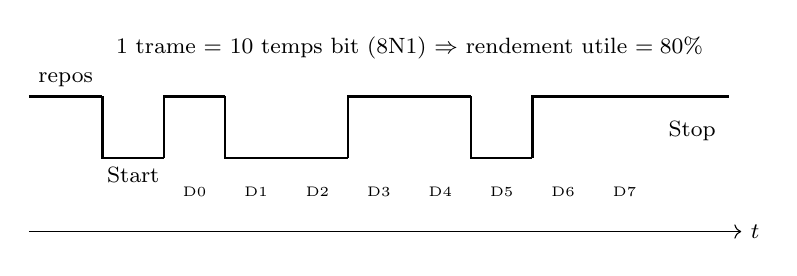
\begin{tikzpicture}[scale=0.78]
  % Ligne au repos (haut)
  \draw[thick] (-1.2,1) -- (0,1);
  \node[above, font=\footnotesize] at (-0.6,1) {repos};
  % Start bit (bas)
  \draw[thick] (0,1) -- (0,0) -- (1,0);
  \node[font=\footnotesize, below] at (0.5,0) {Start};
  % 8 bits de données
  \foreach \i/\lvl/\prev in {1/1/0, 2/0/1, 3/0/0, 4/1/0, 5/1/1, 6/0/1, 7/1/0, 8/1/1}{
    \draw[thick] (\i,\prev) -- (\i,\lvl) -- (\i+1,\lvl);
  }
  \foreach \i/\n in {1/D0, 2/D1, 3/D2, 4/D3, 5/D4, 6/D5, 7/D6, 8/D7}{
    \node[font=\tiny] at (\i+0.5,-0.55) {\n};
  }
  % Stop bit (haut)
  \draw[thick] (9,1) -- (10.2,1);
  \node[font=\footnotesize, below] at (9.6,0.75) {Stop};
  % Axe
  \draw[->] (-1.2,-1.2) -- (10.4,-1.2) node[right, font=\footnotesize]{$t$};
  \node[font=\footnotesize, above] at (5,1.45) {1 trame = 10 temps bit (8N1) $\Rightarrow$ rendement utile $= 80\%$};
\end{tikzpicture}
\end{center}

\begin{itemize}[nosep]
\item \textbf{Repos} : ligne à l'état haut.
\item \textbf{Bit de start} (passage à 0) : c'est \textit{ce front descendant} qui synchronise le récepteur. Il échantillonne ensuite chaque bit \textit{au milieu} de son temps bit.
\item 8 bits de données (LSB en premier), parité optionnelle, 1--2 bits de stop (retour à 1).
\end{itemize}
\end{formule}

\begin{attention}
\textbf{La contrainte cachée : la tolérance d'horloge.} Le récepteur compte les temps bit avec \textit{sa propre} horloge. L'erreur s'accumule du start jusqu'au dernier bit ($\sim 9{,}5$ temps bit). Pour échantillonner le dernier bit encore dans sa fenêtre ($\pm 1/2$ temps bit), il faut :
\[
\frac{\Delta f}{f} < \frac{0{,}5}{9{,}5} \approx 5\% \;\;\text{au total, soit} \;\; \boxed{< 2{,}5\% \text{ par horloge}}
\]
C'est pour cela qu'un oscillateur RC interne ($\pm 1$--$2\%$) suffit \textit{tout juste} pour l'UART, et que les trames longues (9 bits + parité) réduisent encore la marge. Un quartz règle définitivement la question.
\end{attention}

\subsection{Le SPI : la simplicité synchrone}

\begin{formule}
\textbf{SPI} (\textit{Serial Peripheral Interface}) : un \textbf{maître} et un ou plusieurs \textbf{esclaves}, quatre fils :
\begin{itemize}[nosep]
\item \textbf{SCLK} : l'horloge, générée par le maître --- plus de problème de tolérance d'horloge.
\item \textbf{MOSI} (\textit{Master Out, Slave In}) et \textbf{MISO} : les deux sens de données --- \textbf{full duplex}.
\item \textbf{CS/SS} (\textit{Chip Select}) : un fil par esclave, actif bas, sélectionne le destinataire.
\end{itemize}

\textbf{Le cœur du SPI est un registre à décalage} (chapitre 21) de chaque côté : à chaque front d'horloge, un bit sort du maître (MOSI) et un bit sort de l'esclave (MISO). Après 8 fronts, les deux registres ont \textbf{échangé} leurs contenus. Il n'y a ni adresse, ni trame, ni acquittement : le protocole, c'est l'application qui le définit.

\textbf{Débits} : 1--100 MHz typiques. Le plus rapide des trois bus de base --- limité par la longueur des pistes et la charge capacitive, pas par le protocole.
\end{formule}

\subsection{L'I\textsuperscript{2}C : deux fils pour tout un système}

\begin{formule}
\textbf{I\textsuperscript{2}C} (\textit{Inter-Integrated Circuit}) : \textbf{deux fils seulement} (SDA données, SCL horloge) partagés par tous les périphériques --- jusqu'à une centaine sur le même bus.

\begin{itemize}[nosep]
\item \textbf{Adressage} : chaque esclave a une adresse sur 7 bits (ou 10). Le maître commence chaque échange par l'adresse visée + un bit lecture/écriture.
\item \textbf{Acquittement (ACK)} : après chaque octet, le récepteur tire SDA à 0 pendant un temps bit. Pas d'ACK $=$ personne à cette adresse, ou esclave saturé.
\item \textbf{Conditions de start/stop} : un front sur SDA \textit{pendant que SCL est haut} (interdit en données) signale le début ou la fin de transaction.
\item \textbf{Débits} : 100 kHz (standard), 400 kHz (fast), 1 MHz (fast+), 3,4 MHz (high-speed, rare).
\end{itemize}

\textbf{Pourquoi si lent ?} La réponse est \textit{électrique} --- c'est la section suivante.
\end{formule}

\begin{retenir}
\textbf{L'essentiel :}
\begin{enumerate}[nosep]
\item Le série a gagné contre le parallèle pour une raison physique : le skew inter-fils.
\item UART : asynchrone, 2 fils, tolérance d'horloge $< 2{,}5\%$ par côté. Simple et universel.
\item SPI : synchrone, full duplex, registres à décalage face à face. Rapide, mais 3+n fils.
\item I\textsuperscript{2}C : 2 fils partagés, adressage, ACK. Lent --- pour une raison électrique (open-drain).
\end{enumerate}
\end{retenir}

% ============================================================================
\section{Approfondissement}

\vspace{0.3cm}
\textit{La couche électrique : pourquoi l'I\textsuperscript{2}C est lent, comment choisir sa pull-up, et ce que cachent les modes SPI.}
\vspace{0.3cm}

\begin{approfondissement}
Open-drain et calcul de pull-up (RC, chapitre 9), modes SPI (CPOL/CPHA), arbitrage I\textsuperscript{2}C, clock stretching. Prérequis : chapitres 9 (RC), 17 (MOSFET), 20 (totem-pole).
\end{approfondissement}

\subsection{Open-drain : le bus partagé sans conflit}

\begin{formule}
\textbf{Le problème :} sur un bus partagé, si deux sorties totem-pole (chapitre 20) parlent en même temps --- l'une à 1, l'autre à 0 --- un court-circuit $V_{DD} \to$ masse traverse les deux étages de sortie : la \textit{bus contention} du chapitre 26.

\textbf{La solution I\textsuperscript{2}C : l'open-drain.} Chaque sortie n'a \textit{que} le NMOS de pull-down (chapitre 17). Personne ne \textit{force} le niveau haut : c'est une \textbf{résistance de pull-up} commune $R_p$ qui ramène la ligne à $V_{DD}$ quand tout le monde la relâche.
\begin{itemize}[nosep]
\item N'importe qui peut tirer la ligne à 0 (\textbf{ET câblé}, \textit{wired-AND}) : aucun conflit destructif possible.
\item Le niveau bas est \textit{dominant}, le niveau haut \textit{récessif} --- cette asymétrie est la base de l'arbitrage (et on la retrouvera dans le CAN).
\end{itemize}
\end{formule}

\begin{attention}
\textbf{Le prix de l'open-drain : le front montant est un RC.}

La descente est rapide (le NMOS tire fort). Mais la \textbf{montée} n'est pilotée que par $R_p$ qui charge la capacité totale du bus $C_b$ (pistes + entrées de tous les périphériques, $\SI{50}{}$--$\SI{400}{pF}$) :
\[
\boxed{t_{\text{montée}} \approx 0{,}85 \, R_p C_b \quad (\text{de } 30\% \text{ à } 70\% \text{ de } V_{DD})}
\]
C'est exactement la charge du condensateur du chapitre 9. La spécification I\textsuperscript{2}C impose $t_r < \SI{1}{\micro s}$ (100 kHz) ou $< \SI{300}{ns}$ (400 kHz) : c'est \textit{cette constante RC} qui plafonne le débit du bus, pas la logique.

\textbf{Dimensionnement de $R_p$ :}
\begin{itemize}[nosep]
\item \textbf{Maximum} (vitesse) : $R_{p,\max} = t_{r,\max}/(0{,}85\,C_b)$.
\item \textbf{Minimum} (courant) : le NMOS doit pouvoir tenir le niveau bas sous $V_{OL} < \SI{0.4}{V}$ avec $I_{OL} \leq \SI{3}{mA}$ : $R_{p,\min} = (V_{DD}-0{,}4)/\SI{3}{mA}$ ($\approx \SI{1}{k\ohm}$ sous \SI{3.3}{V}).
\end{itemize}
Entre les deux, on choisit \textit{bas} pour la vitesse, \textit{haut} pour la consommation (le courant $V_{DD}/R_p$ circule à chaque niveau bas).
\end{attention}

\subsection{Les quatre modes SPI : CPOL et CPHA}

\begin{formule}
Deux paramètres définissent \textit{quand} les bits sont posés et capturés :
\begin{itemize}[nosep]
\item \textbf{CPOL} (polarité) : niveau de repos de SCLK (0 ou 1).
\item \textbf{CPHA} (phase) : capture sur le \textit{premier} front (CPHA=0) ou le \textit{second} (CPHA=1) de chaque période.
\end{itemize}

\begin{center}
\renewcommand{\arraystretch}{1.35}
\begin{tabular}{p{1.5cm}p{1.3cm}p{1.3cm}p{3.6cm}p{3.6cm}}
\toprule
\textbf{Mode} & \textbf{CPOL} & \textbf{CPHA} & \textbf{Capture sur} & \textbf{Donnée posée sur} \\
\midrule
0 & 0 & 0 & front montant & front descendant \\
1 & 0 & 1 & front descendant & front montant \\
2 & 1 & 0 & front descendant & front montant \\
3 & 1 & 1 & front montant & front descendant \\
\bottomrule
\end{tabular}
\end{center}

Le mode est imposé par \textit{chaque périphérique} (datasheet). Les modes 0 et 3 dominent en pratique. \textbf{90\% des ``SPI qui ne marche pas'' sont un mauvais couple CPOL/CPHA} : à l'oscilloscope, on voit les données décalées d'un demi-bit ou lues sur le mauvais front.
\end{formule}

\subsection{I\textsuperscript{2}C avancé : arbitrage et clock stretching}

\begin{formule}
\textbf{Arbitrage multi-maître :} si deux maîtres démarrent en même temps, chacun \textit{relit} SDA en l'émettant. Celui qui écrit 1 (récessif) mais lit 0 (un autre a tiré la ligne) \textbf{a perdu} : il se retire sans corrompre la trame --- arbitrage \textit{non destructif}, gagné par l'adresse la plus basse.

\textbf{Clock stretching :} un esclave lent peut \textbf{tenir SCL à 0} après un octet : le maître, qui relit SCL avant chaque impulsion, attend. C'est le contrôle de flux le plus simple qui soit --- et une source classique de blocage de bus si l'esclave plante en tenant SCL (parade : compteur de timeout côté maître, et séquence de récupération à 9 impulsions d'horloge).
\end{formule}

\begin{pratique}
\textbf{Réflexe de débogage I\textsuperscript{2}C à l'oscilloscope :}
\begin{enumerate}[nosep]
\item \textbf{Fronts montants mous ?} $\Rightarrow$ $R_p C_b$ trop grand : réduire $R_p$ ou raccourcir le bus.
\item \textbf{Pas d'ACK ?} $\Rightarrow$ mauvaise adresse (décalage 7 bits vs 8 bits : l'erreur n°1), périphérique non alimenté, ou bus bloqué.
\item \textbf{SDA collée à 0 ?} $\Rightarrow$ un esclave est resté au milieu d'une transaction : envoyer 9 impulsions SCL puis un stop.
\item \textbf{Niveaux bas à $\SI{0.8}{V}$ au lieu de $\SI{0.2}{V}$ ?} $\Rightarrow$ $R_p$ trop faible : le NMOS ne tient plus $V_{OL}$.
\end{enumerate}
\end{pratique}

% ============================================================================
\section{Niveau Ingénieur}

\begin{ingenieur}
La signalisation différentielle (CAN, RS-485, USB), l'arbitrage CAN, et le choix raisonné d'un protocole. Liens : chapitre 16 (paire différentielle), chapitre 22 (CDC), partie IX à venir (intégrité du signal).
\end{ingenieur}

\subsection{La signalisation différentielle : l'immunité par construction}

\begin{formule}
UART, SPI et I\textsuperscript{2}C sont \textit{single-ended} : le niveau est mesuré par rapport à la masse. Sur quelques centimètres de PCB, très bien. Sur des mètres de câble dans un environnement industriel ou automobile, la masse elle-même bouge (chutes ohmiques, boucles --- partie IX) et les parasites s'additionnent au signal.

\textbf{La parade : transmettre la \textit{différence}.} Deux fils portent $V_+$ et $V_-$ en opposition ; le récepteur ne lit que $V_+ - V_-$ :
\begin{itemize}[nosep]
\item Un parasite couplé sur le câble touche \textit{les deux fils ensemble} (mode commun) $\Rightarrow$ il disparaît dans la soustraction.
\item Le récepteur est\ldots une \textbf{paire différentielle} (chapitre 16) : la réjection de mode commun (CMRR) du montage devient l'immunité du bus.
\item En torsadant la paire, on garantit que les deux fils voient le \textit{même} environnement électromagnétique.
\end{itemize}

\textbf{Trois standards différentiels majeurs :} RS-485 (industriel, $\pm\SI{1.5}{V}$ min, 32+ nœuds, jusqu'à \SI{1200}{m}), CAN (automobile), USB (grand public).
\end{formule}

\subsection{Le bus CAN : l'arbitrage par la physique}

\begin{formule}
\textbf{CAN} (\textit{Controller Area Network}) : le bus de l'automobile et de l'industrie. Deux fils (CANH, CANL), terminés par $\SI{120}{\ohm}$ à chaque extrémité.

\textbf{Deux états --- la version différentielle de l'open-drain :}
\begin{itemize}[nosep]
\item \textbf{Récessif} (bit 1) : aucun émetteur ne pilote, les deux fils au repos ($V_{\text{diff}} \approx 0$).
\item \textbf{Dominant} (bit 0) : un émetteur écarte les deux fils ($V_{\text{diff}} \approx \SI{2}{V}$). \textbf{Le dominant gagne toujours sur le récessif} --- exactement le wired-AND de l'I\textsuperscript{2}C, en différentiel.
\end{itemize}

\textbf{Arbitrage non destructif :} chaque trame commence par un \textbf{identifiant} (11 ou 29 bits) qui est aussi sa \textbf{priorité}. Tous les nœuds peuvent émettre en même temps : chacun relit le bus bit à bit, et celui qui émet récessif mais lit dominant se retire immédiatement. \textbf{L'identifiant le plus bas (le plus de zéros en tête) gagne, sans perdre un seul bit de temps.} Le message le plus prioritaire (freinage\ldots) passe toujours en premier : déterminisme par construction physique.

\textbf{Robustesse :} CRC 15 bits, acquittement par \textit{tous} les récepteurs, \textit{bit stuffing} (un bit inverse inséré après 5 bits identiques pour maintenir la synchronisation), et confinement automatique des nœuds défaillants (compteurs d'erreurs TEC/REC). Débit : \SI{1}{Mbit/s} (classique), \SI{8}{Mbit/s} (CAN FD).
\end{formule}

\begin{intuition}
\textbf{La contrainte cachée du CAN : la longueur du bus.} L'arbitrage exige que \textit{tous} les nœuds voient le même bit \textit{pendant} le temps bit : un nœud à l'autre bout doit recevoir le dominant, et sa réponse doit revenir, en moins d'un temps bit. À \SI{1}{Mbit/s} ($T_{\text{bit}} = \SI{1}{\micro s}$, propagation $\sim\SI{5}{ns/m}$ aller-retour $\times 2$), la limite est $\sim\SI{40}{m}$. À \SI{125}{kbit/s} : $\sim\SI{500}{m}$. \textbf{Le produit débit $\times$ longueur est borné par la vitesse de la lumière} --- aucune astuce de protocole n'y échappe.
\end{intuition}

\subsection{USB : l'essentiel pour l'électronicien}

\begin{formule}
\textbf{USB} (\textit{Universal Serial Bus}) : paire différentielle D+/D$-$, codage \textbf{NRZI} avec bit stuffing (l'horloge est extraite des transitions des données --- pas de fil d'horloge), topologie en étoile via hubs, et \textbf{énumération} : à la connexion, l'hôte interroge le périphérique (descripteurs) et lui attribue une adresse.

\textbf{Ce que l'électronicien doit retenir :}
\begin{itemize}[nosep]
\item \textbf{Détection de vitesse par pull-up} : une résistance de $\SI{1.5}{k\ohm}$ sur D+ (full-speed, \SI{12}{Mbit/s}) ou D$-$ (low-speed) signale la présence et la vitesse. En high-speed (\SI{480}{Mbit/s}), négociation électrique supplémentaire (\textit{chirp}).
\item \textbf{Impédance contrôlée} : la paire D+/D$-$ doit être routée à $\SI{90}{\ohm}$ différentiel, longueurs appariées --- premier contact avec l'intégrité du signal de la partie IX.
\item \textbf{Alimentation} : \SI{5}{V}, négociation de courant (100/500 mA, et bien plus en USB-C Power Delivery).
\end{itemize}
\end{formule}

\subsection{Choisir son protocole}

\begin{pratique}
\begin{center}
\renewcommand{\arraystretch}{1.4}
\begin{tabular}{p{1.4cm}p{1.1cm}p{1.9cm}p{2.0cm}p{2.1cm}p{2.7cm}}
\toprule
\textbf{Bus} & \textbf{Fils} & \textbf{Débit typ.} & \textbf{Portée} & \textbf{Topologie} & \textbf{Point fort} \\
\midrule
UART & 2 & $\leq$ 1 Mbit/s & quelques m & point à point & simplicité, universel \\
SPI & 3+$n$ & 1--100 MHz & PCB & maître/\allowbreak esclaves & vitesse, full duplex \\
I\textsuperscript{2}C & 2 & 0,1--1 Mbit/s & PCB ($<$ 1 m) & multi-nœuds & économie de fils \\
CAN & 2 & 0,125--8 Mbit/s & 40--500 m & multi-maître & robustesse, priorités \\
RS-485 & 2 & $\leq$ 10 Mbit/s & 1200 m & multi-nœuds & distance, industriel \\
USB & 2--4 & 12--480+ Mbit/s & 5 m & étoile (hôte) & débit, grand public \\
\bottomrule
\end{tabular}
\end{center}

\textbf{Réflexes :} capteur sur le même PCB $\to$ I\textsuperscript{2}C (lent, peu de fils) ou SPI (rapide). Console de debug $\to$ UART. Câble dans une machine $\to$ CAN ou RS-485 (différentiel obligatoire dès que la masse n'est plus commune et propre). Vers un PC $\to$ USB.
\end{pratique}

\subsection{La traversée de domaine d'horloge, encore}

\begin{intuition}
Chaque récepteur série est un \textbf{problème de CDC} (chapitre 22) : les données arrivent au rythme de l'horloge \textit{de l'émetteur}, et doivent entrer dans le domaine d'horloge \textit{local}. Le bit RX d'un UART traverse systématiquement un synchroniseur double bascule avant la FSM de réception (chapitre 23) ; les contrôleurs SPI esclaves resynchronisent SCLK ; les PHY USB et CAN intègrent des CDR (\textit{Clock and Data Recovery}, des PLL qui se verrouillent sur les transitions --- chapitre 22). \textbf{Un protocole série est une FSM + un synchroniseur + une couche électrique} : tout ce chapitre est l'assemblage des trois précédents.
\end{intuition}

% === EXERCICES ===
\section*{Exercices}
\addcontentsline{toc}{section}{Exercices}

\subsection*{Niveau débutant}

\textbf{Exercice 28.1 ---} Un UART configuré en 115200 bauds, 8N1 (8 bits, sans parité, 1 stop). Quel est le débit \textit{utile} en octets par seconde ? Combien de temps pour transmettre 1 ko ?

\begin{pratique}
\textbf{Solution :} 1 trame $=$ 10 temps bit pour 8 bits utiles. Débit utile $= 115200 \times 8/10 = \SI{92160}{bits/s} = \SI{11.52}{ko/s}$.

1 ko $= 1024$ octets $\Rightarrow t = 1024/11520 \approx \SI{89}{ms}$. L'UART est lent : c'est le prix de la simplicité.
\end{pratique}

\textbf{Exercice 28.2 ---} Un capteur I\textsuperscript{2}C a l'adresse 7 bits 0x48. Quel octet le maître émet-il pour le lire ? Pour lui écrire ? (Convention : adresse décalée + bit R/$\overline{\text{W}}$.)

\begin{pratique}
\textbf{Solution :} l'octet d'adresse $=$ adresse $\ll 1$ $|$ R/$\overline{\text{W}}$. $0x48 \ll 1 = 0x90$.

Écriture (R/$\overline{\text{W}} = 0$) : \textbf{0x90}. Lecture (R/$\overline{\text{W}} = 1$) : \textbf{0x91}.

C'est l'ambiguïté classique des datasheets : certaines annoncent ``0x90'' (adresse 8 bits), d'autres ``0x48'' (7 bits). Un facteur 2 d'écart $\Rightarrow$ pas d'ACK $\Rightarrow$ vérifier systématiquement.
\end{pratique}

\subsection*{Niveau intermédiaire}

\textbf{Exercice 28.3 ---} Un bus I\textsuperscript{2}C sous $V_{DD} = \SI{3.3}{V}$ a une capacité totale $C_b = \SI{200}{pF}$. La spécification fast-mode (400 kHz) impose $t_r < \SI{300}{ns}$ et $I_{OL,\max} = \SI{3}{mA}$ avec $V_{OL} = \SI{0.4}{V}$.

(a) Calculez $R_{p,\max}$ et $R_{p,\min}$.

(b) Quelle valeur normalisée choisir, et quelle est la consommation au niveau bas ?

\begin{pratique}
\textbf{Solution :}

(a) $R_{p,\max} = t_r/(0{,}85\,C_b) = 300\times10^{-9}/(0{,}85\times200\times10^{-12}) = \SI{1.76}{k\ohm}$.

$R_{p,\min} = (3{,}3-0{,}4)/3\times10^{-3} = \SI{0.97}{k\ohm}$.

(b) Fenêtre $[0{,}97 ; 1{,}76]\,\si{k\ohm}$ : on prend $R_p = \SI{1.5}{k\ohm}$ (E12, marge des deux côtés).

Consommation par ligne au niveau bas : $I = 3{,}3/1500 = \SI{2.2}{mA}$. Avec SDA et SCL souvent à 0 pendant les transferts : quelques mA en continu --- non négligeable sur pile, d'où l'intérêt de bus rapides et de transactions courtes.
\end{pratique}

\textbf{Exercice 28.4 ---} La datasheet d'un convertisseur indique : ``SCLK idle high, data latched on rising edge''. Quel mode SPI configurer ? Que voit-on à l'oscilloscope si on se trompe et qu'on configure le mode 0 ?

\begin{pratique}
\textbf{Solution :} repos haut $\Rightarrow$ CPOL $= 1$. Capture sur front montant avec CPOL $=1$ : le front montant est le \textit{second} front de la période $\Rightarrow$ CPHA $= 1$. \textbf{Mode 3}.

En mode 0 par erreur : l'horloge repose à 0 et capture sur le \textit{premier} front montant. Le périphérique, lui, pose ses bits par rapport à son repos haut : à l'oscilloscope, les données semblent \textbf{décalées d'un bit} (le premier bit lu est un fantôme du repos) --- le symptôme typique : ``je lis 0x80 au lieu de 0x01'', tout est décalé d'un cran.
\end{pratique}

\subsection*{Niveau ingénieur}

\textbf{Exercice 28.5 ---} Deux nœuds CAN démarrent simultanément : le nœud A avec l'identifiant 0x12C (0b00100101100), le nœud B avec 0x130 (0b00100110000). Qui gagne l'arbitrage, et au bout de combien de bits ?

\begin{pratique}
\textbf{Solution :} comparaison bit à bit (MSB en premier, dominant $= 0$ gagne) :

\begin{center}
\begin{tabular}{lccccccc}
bit & 10 & 9 & 8 & 7 & 6 & 5 & 4 \\
A (0x12C) & 0 & 0 & 1 & 0 & 0 & 1 & 0 \\
B (0x130) & 0 & 0 & 1 & 0 & 0 & 1 & 1 \\
\end{tabular}
\end{center}

Identiques jusqu'au bit 5 inclus. \textbf{Au bit 4} : A émet 0 (dominant), B émet 1 (récessif) mais relit 0 $\Rightarrow$ \textbf{B se retire, A gagne} après 7 bits d'arbitrage. A (0x12C $<$ 0x130) est bien le plus prioritaire, et B retentera automatiquement dès la fin de la trame de A --- aucun temps de bus perdu.
\end{pratique}

\textbf{Exercice 28.6 ---} Un UART récepteur utilise un oscillateur RC à $\pm 1{,}5\%$. L'émetteur est à $\pm 1\%$. La trame fait 8N1, et le récepteur échantillonne au milieu théorique de chaque bit.

(a) L'accumulation d'erreur sur le dernier bit (9,5 temps bit) reste-t-elle dans la fenêtre de $\pm 0{,}5$ temps bit ?

(b) Et avec une trame 9 bits + parité (11,5 temps bit) ?

\begin{pratique}
\textbf{Solution :}

(a) Erreur relative pire cas : $1{,}5 + 1 = 2{,}5\%$. Dérive au dernier échantillon : $9{,}5 \times 0{,}025 = 0{,}238$ temps bit $< 0{,}5$. \textbf{OK}, avec une marge de 52\% (qui absorbe aussi la distorsion des fronts).

(b) $11{,}5 \times 0{,}025 = 0{,}288$ temps bit $< 0{,}5$ : encore OK, marge 42\%. Mais si l'oscillateur RC dérive en température à $\pm 2{,}5\%$ : $11{,}5\times0{,}035 = 0{,}40$ --- la marge fond à 20\%, et les fronts mous d'un câble long la consomment. \textbf{Règle pratique : au-delà de $\pm 2\%$ cumulés, passer au quartz.}
\end{pratique}

\subsection*{Questions de compréhension}

\begin{enumerate}[nosep]
\item Pourquoi le front montant de l'I\textsuperscript{2}C est-il lent alors que le front descendant est rapide ? Reliez chaque front à son ``moteur'' électrique ($R_p$ vs NMOS).
\item Le CAN et l'I\textsuperscript{2}C utilisent tous deux un état dominant et un état récessif. Quel mécanisme cela rend-il possible dans les deux cas, et pourquoi est-il \textit{non destructif} ?
\item Le SPI n'a ni adresse, ni ACK, ni CRC. Dans quelles conditions est-ce acceptable, et qu'est-ce qui doit compenser quand ça ne l'est plus ?
\item Pourquoi le produit débit $\times$ longueur d'un bus CAN est-il physiquement borné ? Que se passerait-il si on violait cette limite pendant l'arbitrage ?
\end{enumerate}

% === RÉSUMÉ ===
\section*{Résumé du chapitre}
\addcontentsline{toc}{section}{Résumé du chapitre}

\begin{bases}[title={\color{white} Résumé --- Les Bases}]
\begin{center}
\renewcommand{\arraystretch}{1.3}
\begin{tabular}{p{3.5cm}p{9.5cm}}
\toprule
Série $>$ parallèle & Le skew inter-fils condamne le parallèle à haut débit \\
UART & Asynchrone, start/stop, tolérance d'horloge $< 2{,}5\%$/côté \\
SPI & Synchrone, full duplex, deux registres à décalage face à face (Ch.21) \\
I\textsuperscript{2}C & 2 fils partagés, adresses 7 bits, ACK, wired-AND \\
\bottomrule
\end{tabular}
\end{center}
\end{bases}

\begin{approfondissement}[title={\color{white} Résumé --- Approfondissement}]
\begin{center}
\renewcommand{\arraystretch}{1.3}
\begin{tabular}{p{3.5cm}p{9.5cm}}
\toprule
Open-drain & Bas dominant, haut récessif. Montée $= 0{,}85\,R_p C_b$ (Ch.9) : c'est elle qui limite le débit \\
Pull-up & $R_{p,\min}$ (tenir $V_{OL}$) $< R_p < R_{p,\max}$ (tenir $t_r$) \\
Modes SPI & CPOL/CPHA : 90\% des pannes SPI. Modes 0 et 3 dominants \\
I\textsuperscript{2}C avancé & Arbitrage non destructif, clock stretching, récupération 9 clocks \\
\bottomrule
\end{tabular}
\end{center}
\end{approfondissement}

\begin{ingenieur}[title={\color{white} Résumé --- Niveau Ingénieur}]
\begin{center}
\renewcommand{\arraystretch}{1.3}
\begin{tabular}{p{3.5cm}p{9.5cm}}
\toprule
Différentiel & Le parasite est en mode commun $\Rightarrow$ rejeté par la paire diff (Ch.16). RS-485, CAN, USB \\
CAN & Dominant/récessif différentiel, arbitrage par identifiant = priorité, CRC + ACK + stuffing \\
Limite physique & Débit $\times$ longueur borné par la propagation (arbitrage en 1 temps bit) \\
USB & NRZI + CDR, pull-up de détection, $\SI{90}{\ohm}$ différentiel (annonce partie IX) \\
CDC & Tout récepteur série $=$ synchroniseur (Ch.22) $+$ FSM (Ch.23) $+$ couche électrique \\
\bottomrule
\end{tabular}
\end{center}
\end{ingenieur}


% ============================================================================
% CHAPITRE 29 : LIMITES PHYSIQUES DU NUMÉRIQUE
% VERSION PEER-REVIEW
% Fichier autonome à intégrer dans Bible_Elec.tex
% ============================================================================

\chapter{Limites physiques du numérique}

\begin{center}
\textit{Pendant cinquante ans, le numérique a semblé défier la physique :\\
deux fois plus de transistors tous les deux ans, toujours plus vite,\\
sans jamais payer le prix. Cette époque est terminée.\\
Le bruit, la chaleur, la variabilité et le vieillissement\\
sont revenus dicter leurs conditions. Ce chapitre clôt la partie numérique\\
en montrant où sont les murs --- et comment l'ingénieur compose avec.}
\end{center}

\vspace{0.5cm}

Les chapitres 20 à 28 ont construit le numérique comme si les transistors étaient parfaits, identiques et éternels. Ils ne le sont pas. Ce chapitre rassemble les limites physiques qui gouvernent la conception moderne : le \textbf{bruit} (chapitres 16--17) qui fixe un plancher, la \textbf{consommation} (chapitre 20) qui fixe un plafond, la \textbf{variabilité} (chapitres 22, 24) qui mange les marges, et le \textbf{vieillissement} qui dégrade tout dans le temps. C'est la synthèse physique de toute la partie VI --- et la raison d'être des parties suivantes (alimentations, CEM).

% ============================================================================
\section{Les Bases}

\begin{bases}
La fin du scaling idéal, le plancher du bruit, et le mur de la consommation. Prérequis : chapitres 17 ($I_{\text{off}}$), 20 ($P = \alpha C V^2 f$).
\end{bases}

\subsection{L'âge d'or : la loi de Moore et le scaling de Dennard}

\begin{formule}
\textbf{Loi de Moore} (1965, observation économique) : le nombre de transistors par puce double tous les $\sim 2$ ans.

\textbf{Scaling de Dennard} (1974, la physique qui rendait Moore \textit{gratuit}) : en réduisant toutes les dimensions et la tension d'un facteur $k \approx 0{,}7$ à chaque génération :
\[
L' = kL, \quad V'_{DD} = kV_{DD}, \quad C' = kC
\]
\begin{itemize}[nosep]
\item Délai des portes : $\times k$ ($\Rightarrow$ fréquence $\times 1/k \approx +40\%$).
\item Puissance par transistor : $\times k^2$ via $CV^2f$.
\item \textbf{Densité de puissance (W/mm$^2$) : constante.} On pouvait doubler les transistors ET monter la fréquence sans chauffer plus.
\end{itemize}
\end{formule}

\begin{attention}
\textbf{La fin de Dennard ($\sim$ 2005) :} $V_{DD}$ ne peut plus descendre. Deux raisons physiques :
\begin{itemize}[nosep]
\item $V_{th}$ ne peut pas suivre : la pente sous-seuil est bornée à $\SI{60}{mV/décade}$ à \SI{300}{K} (limite thermodynamique $kT/q\cdot\ln 10$, chapitre 17). Baisser $V_{th}$ fait exploser $I_{\text{off}}$ \textbf{exponentiellement}.
\item Sans baisser $V_{th}$, baisser $V_{DD}$ écrase la marge $V_{DD} - V_{th}$ : les portes deviennent lentes.
\end{itemize}
$V_{DD}$ est bloquée autour de $0{,}7$--$\SI{1}{V}$ depuis 15 ans. Conséquence : chaque génération ajoute des transistors \textbf{sans} réduire leur énergie d'autant $\Rightarrow$ la densité de puissance \textit{augmente}. C'est la cause directe du plafonnement des fréquences à $\sim\SI{4}{}$--$\SI{5}{GHz}$ (le Pentium 4 en a été la première victime, chapitre 26) et de la bascule vers le multicœur.
\end{attention}

\subsection{Le plancher : le bruit}

\begin{formule}
On ne peut pas réduire indéfiniment l'énergie d'un bit, car le bruit thermique fixe un plancher.

\textbf{Le bruit $kTC$} : toute capacité échantillonnée porte une incertitude de tension (chapitres 17, 27) :
\[
\boxed{\sigma_V = \sqrt{\frac{kT}{C}}}
\]
$C = \SI{1}{fF}$ à \SI{300}{K} : $\sigma_V = \SI{2}{mV}$. $C = \SI{1}{aF}$ (transistor ultime) : $\sigma_V = \SI{64}{mV}$ --- comparable aux niveaux logiques d'un circuit sous \SI{0.5}{V} !

\textbf{L'énergie minimale d'une commutation fiable} : pour qu'un bit soit distinguable du bruit avec un taux d'erreur acceptable, il faut $E_{\text{bit}} \gg kT\ln 2 \approx \SI{3e-21}{J}$ (limite de Landauer). Les circuits 2024 commutent à $\sim 10^{-15}$--$10^{-16}\,$J par porte : encore $10^4$--$10^5 \times$ au-dessus de la limite --- mais la marge se réduit de génération en génération, et le \textit{rapport signal/bruit} des nœuds internes, lui, se dégrade déjà (mémoires, chapitre 24 ; ADC, chapitre 27).
\end{formule}

\subsection{Le plafond : le mur de la consommation}

\begin{formule}
\textbf{Le budget thermique d'une puce est borné} : $\sim\SI{100}{W}$ pour un CPU desktop avec radiateur, $\sim\SI{5}{W}$ pour un smartphone, $\sim\SI{100}{mW}$ pour un objet IoT sur pile. Rappel du chapitre 20 :
\[
P_{\text{totale}} = \underbrace{\alpha C V_{DD}^2 f}_{\text{dynamique}} + \underbrace{V_{DD}\, I_{\text{off}}\, N}_{\text{statique}}
\]
\begin{itemize}[nosep]
\item La dynamique se paie \textbf{à chaque commutation} : elle plafonne $f$.
\item La statique se paie \textbf{en permanence} : avec $N \sim 10^{10}$ transistors et $I_{\text{off}}$ qui double tous les \SI{10}{°C} (chapitre 17), elle représente $20$--$40\%$ du total en technologie avancée --- et elle s'auto-amplifie avec la température (fuite $\to$ chaleur $\to$ fuite).
\end{itemize}
\end{formule}

\begin{retenir}
\textbf{L'essentiel :}
\begin{enumerate}[nosep]
\item Dennard est mort ($\sim$ 2005) : $V_{DD}$ est bloquée par la pente sous-seuil ($\SI{60}{mV/dec}$, thermodynamique).
\item Plancher : bruit $\sqrt{kT/C}$ --- les petits nœuds deviennent bruyants.
\item Plafond : budget thermique fixe + fuites croissantes $\Rightarrow$ fréquences plafonnées, multicœur obligatoire.
\item Tout le reste du chapitre découle de ces trois faits.
\end{enumerate}
\end{retenir}

% ============================================================================
\section{Approfondissement}

\vspace{0.3cm}
\textit{La variabilité : pourquoi deux transistors ``identiques'' ne le sont jamais, et ce que cela coûte en marges de conception.}
\vspace{0.3cm}

\begin{approfondissement}
Variabilité de fabrication (RDF, LER), corners PVT, et le coût des marges. Prérequis : chapitres 17, 22 (corners), 24 (SNM).
\end{approfondissement}

\subsection{La variabilité de fabrication : la loi des petits nombres}

\begin{formule}
\textbf{RDF (Random Dopant Fluctuation)} : le canal d'un transistor \SI{7}{nm} contient quelques \textbf{dizaines} d'atomes dopants. Leur nombre exact suit une statistique de Poisson : $\sigma_N = \sqrt{N}$. Avec $N = 50$ : $\pm 14\%$ de variation \textit{naturelle} d'un transistor à l'autre $\Rightarrow$ dispersion de $V_{th}$ :
\[
\sigma_{V_{th}} \approx \frac{A_{VT}}{\sqrt{W L}} \qquad (A_{VT} \sim 1\text{--}\SI{2}{mV\cdot\micro m} \text{ : loi de Pelgrom})
\]
Plus le transistor est \textbf{petit}, plus il est \textbf{dispersé}. À surface minimale en \SI{7}{nm} : $\sigma_{V_{th}} \sim 20$--$\SI{40}{mV}$ --- sur un $V_{th}$ de $\SI{300}{mV}$.

\textbf{LER (Line Edge Roughness)} : les bords de grille, dessinés par lithographie à \SI{193}{nm} (ou EUV \SI{13.5}{nm}) sur des motifs de \SI{20}{nm}, sont rugueux à l'échelle de quelques nm $\Rightarrow$ variation de $L$ effectif, donc de courant et de fuite.

\textbf{Conséquences déjà rencontrées :} l'offset du sense amplifier (chapitre 24), les cellules SRAM faibles (chapitre 24, exercice 24.6), le mésappariement des DAC (chapitre 27, exercice 27.6). \textbf{La variabilité est le même phénomène partout.}
\end{formule}

\subsection{PVT : concevoir pour le pire cas}

\begin{formule}
Rappel du chapitre 22, vu maintenant comme une \textit{conséquence} de la physique :
\begin{itemize}[nosep]
\item \textbf{P (process)} : RDF + LER + gradients de fabrication $\Rightarrow$ puces ``rapides'' (FF) et ``lentes'' (SS) dans le même lot.
\item \textbf{V (voltage)} : l'alimentation réelle varie de $\pm 5$--$10\%$ (chutes ohmiques, transitoires --- ce sera la partie VII).
\item \textbf{T (température)} : $-40$ à $+125\,$°C en automobile. La mobilité baisse avec $T$ (plus lent), $I_{\text{off}}$ explose (plus de fuite), $V_{th}$ baisse.
\end{itemize}

\textbf{Le coût des marges :} un circuit doit fonctionner au coin SS/$V_{\min}$/$T_{\max}$. L'écart de vitesse entre le pire et le meilleur coin atteint $\times 2$ à $\times 3$ en technologie avancée. \textbf{La puce typique tourne donc bien en dessous de ce qu'elle ``pourrait''} : la marge PVT est de la performance sacrifiée à la variabilité.
\end{formule}

\begin{intuition}
\textbf{Les parades modernes transforment la marge statique en adaptation dynamique :}
\begin{itemize}[nosep]
\item \textbf{Binning} : trier les puces après test (les FF deviennent le modèle ``haut de gamme'' --- c'est littéralement la même puce vendue à deux prix).
\item \textbf{DVFS} (\textit{Dynamic Voltage and Frequency Scaling}) : adapter $V_{DD}$ et $f$ à la charge en temps réel. Comme $P_{\text{dyn}} \propto V^2 f$ et que $f_{\max} \propto (V-V_{th})$, baisser les deux ensemble gagne en \textbf{cube} de la tension à performance réduite.
\item \textbf{Capteurs sur puce} : des oscillateurs en anneau répartis mesurent la vitesse \textit{réelle} de chaque zone ; le contrôleur ajuste $V_{DD}$ au plus juste (AVS, \textit{Adaptive Voltage Scaling}).
\end{itemize}
\end{intuition}

% ============================================================================
\section{Niveau Ingénieur}

\begin{ingenieur}
Le vieillissement (NBTI, HCI, électromigration, TDDB), le dark silicon, et les stratégies de l'ère post-Dennard. Liens : chapitre 17 (porteurs chauds), chapitre 26 (multicœur).
\end{ingenieur}

\subsection{Le vieillissement : les transistors s'usent}

\begin{formule}
Un circuit neuf et le même circuit après 10 ans ne sont pas identiques. Quatre mécanismes dominent :

\textbf{1. NBTI / PBTI (Bias Temperature Instability)} : sous polarisation de grille et à chaud, des charges se piègent à l'interface Si/oxyde $\Rightarrow$ $|V_{th}|$ \textbf{dérive} lentement ($\sim \SI{30}{}$--$\SI{50}{mV}$ sur la durée de vie). Le NBTI frappe les PMOS (grille à 0), le PBTI les NMOS high-k. Partiellement \textit{récupérable} quand la contrainte cesse --- d'où une dérive qui dépend du \textbf{taux d'activité} du signal.

\textbf{2. HCI (Hot Carrier Injection)} : les porteurs chauds du pincement (chapitre 17) s'injectent dans l'oxyde côté drain à chaque commutation $\Rightarrow$ dégradation cumulative de $V_{th}$ et de la pente. Frappe les transistors qui \textbf{commutent beaucoup} (horloges, buffers).

\textbf{3. Électromigration (EM)} : dans les interconnexions, le ``vent d'électrons'' arrache des atomes de métal $\Rightarrow$ vides (circuits ouverts) ou excroissances (courts-circuits). Loi de Black :
\[
\boxed{MTTF = \frac{A}{J^n}\, e^{E_a/kT}} \qquad (n \approx 2, \; E_a \approx \SI{0.8}{eV} \text{ pour le cuivre})
\]
Doubler la densité de courant $J$ divise la durée de vie par $\sim 4$ ; $+\SI{25}{°C}$ la divise par $\sim 5$. C'est \textbf{la} contrainte de dimensionnement des rails d'alimentation ($J_{\max} \sim \SI{1}{}$--$\SI{2}{MA/cm^2}$).

\textbf{4. TDDB (Time-Dependent Dielectric Breakdown)} : l'oxyde de grille ($\sim\SI{1}{nm}$ !) accumule des défauts sous champ jusqu'au claquage --- le même mécanisme qui use la Flash (chapitre 24), à l'œuvre partout.
\end{formule}

\begin{attention}
\textbf{Conséquence de conception :} les outils de signoff incluent désormais des analyses de vieillissement : le timing doit être respecté \textit{en fin de vie}, avec les $V_{th}$ dérivés. Encore une marge ($\sim 5$--$10\%$ de fréquence) sacrifiée --- et une raison pour laquelle les électroniques automobile et spatiale, qui visent 15--20 ans à haute température, utilisent des nœuds matures (\SI{40}{}--\SI{90}{nm}) plutôt que la pointe.
\end{attention}

\subsection{Le dark silicon : des transistors qu'on ne peut pas allumer}

\begin{formule}
\textbf{Le paradoxe post-Dennard :} Moore continue (les transistors doublent) mais leur énergie unitaire ne baisse plus assez. Le budget thermique étant fixe :
\[
\text{fraction activable} = \frac{P_{\text{budget}}}{N \cdot E_{\text{transistor}} \cdot f} \quad \xrightarrow[\text{générations}]{} \quad \text{décroît}
\]
Dès \SI{8}{nm}, des études (Esmaeilzadeh et al., 2011) prédisaient que \textbf{plus de 50\% de la puce doit rester éteinte} à tout instant à fréquence nominale : c'est le \textbf{dark silicon}.
\end{formule}

\begin{intuition}
\textbf{Comment l'industrie a transformé la contrainte en stratégie :} si on ne peut pas tout allumer, autant remplir la puce de blocs \textbf{spécialisés} dont un seul s'allume à la fois --- chacun étant 10--100$\times$ plus efficace qu'un CPU généraliste sur \textit{sa} tâche. C'est exactement l'anatomie d'un SoC de smartphone : CPU + GPU + NPU + ISP (image) + codecs vidéo + DSP audio + modem\ldots Le dark silicon explique l'explosion des \textbf{accélérateurs} (chapitre 25 : tensor cores, NPU) et le déclin du ``tout-CPU''. La sobriété imposée par la physique a redessiné l'architecture (chapitre 26).
\end{intuition}

\subsection{Les stratégies de l'ère post-Dennard}

\begin{pratique}
\textbf{La boîte à outils du concepteur contraint --- par ordre de levier :}
\begin{enumerate}[nosep]
\item \textbf{Spécialisation} : un accélérateur dédié gagne $10$--$100\times$ en énergie/opération (le levier dominant).
\item \textbf{DVFS + power gating} : adapter tension/fréquence à la charge ; couper \textit{complètement} l'alimentation des blocs inactifs (transistors d'isolement) pour tuer la fuite --- vital en IoT (chapitre 17 : $I_{\text{off}}$).
\item \textbf{Near-threshold computing} : opérer à $V_{DD} \approx V_{th}$ divise l'énergie par $\sim 10$, au prix d'une vitesse $\div 10$ et d'une sensibilité extrême à la variabilité (la SRAM est la première à lâcher, chapitre 24).
\item \textbf{Empilement 3D} : HBM (chapitre 24), chiplets --- rapprocher mémoire et calcul réduit l'énergie de \textit{transport} des données, devenue dominante (déplacer 64 bits de la DRAM coûte $\sim 100\times$ l'énergie de les additionner).
\item \textbf{Parallélisme large et lent} : $n$ cœurs à $f/n$ consomment moins qu'un cœur à $f$ (le $V^2$ joue pour nous) --- quand l'algorithme s'y prête (loi d'Amdahl).
\end{enumerate}
\end{pratique}

\subsection{Synthèse : la partie VI en une page}

\begin{intuition}
\textbf{La chaîne causale complète du numérique réel :}

La physique du transistor (chapitre 17 : $I_{\text{off}}$, $\SI{60}{mV/dec}$, porteurs chauds) fixe les délais et les fuites $\to$ qui fixent le timing (chapitres 20--22) $\to$ qui contraint les architectures (chapitres 23--26 : pipeline, hiérarchie mémoire, multicœur) $\to$ tandis que le bruit et la variabilité (ce chapitre) limitent les marges des mémoires (chapitre 24) et des convertisseurs (chapitre 27) $\to$ et que le budget thermique (ce chapitre) impose la spécialisation (dark silicon) et la gestion fine de l'énergie. \textbf{Aucun de ces étages n'est ``de l'informatique'' : tout est de l'électronique.} Et la gestion de l'énergie qui vient d'apparaître partout en filigrane mérite sa propre partie : les \textbf{alimentations} (partie VII).
\end{intuition}

% === EXERCICES ===
\section*{Exercices}
\addcontentsline{toc}{section}{Exercices}

\subsection*{Niveau débutant}

\textbf{Exercice 29.1 ---} Un nœud interne a une capacité de $\SI{0.5}{fF}$. Calculez le bruit $kTC$ à \SI{300}{K} et à \SI{400}{K} ($k = \SI{1.38e-23}{J/K}$). Comparez à une marge de bruit de $\SI{100}{mV}$.

\begin{pratique}
\textbf{Solution :} $\sigma_V(\SI{300}{K}) = \sqrt{1{,}38\times10^{-23}\times300/0{,}5\times10^{-15}} = \sqrt{8{,}28\times10^{-6}} = \SI{2.9}{mV}$.

À \SI{400}{K} : $\times\sqrt{400/300} = \SI{3.3}{mV}$.

Marge $100/2{,}9 \approx 34\sigma$ : confortable. Mais à $C = \SI{0.01}{fF}$ : $\sigma = \SI{20}{mV}$, soit $5\sigma$ seulement --- des erreurs apparaissent ($P(5\sigma) \sim 3\times10^{-7}$ par échantillonnage, des milliers par seconde à \SI{1}{GHz}).
\end{pratique}

\textbf{Exercice 29.2 ---} Un SoC a $N = 5\times10^9$ transistors avec $I_{\text{off}} = \SI{10}{nA}$ chacun à \SI{25}{°C}, sous $V_{DD} = \SI{0.8}{V}$. Calculez la puissance statique à \SI{25}{°C} et à \SI{85}{°C} ($I_{\text{off}}$ double tous les \SI{10}{°C}).

\begin{pratique}
\textbf{Solution :} $P_{25} = 0{,}8 \times 10\times10^{-9} \times 5\times10^9 = \SI{40}{W}$\ldots c'est déjà énorme : en pratique seuls $\sim 10\%$ des transistors sont non power-gatés, soit $\sim\SI{4}{W}$.

À \SI{85}{°C} : $(85-25)/10 = 6$ doublements $\Rightarrow \times 64$. $P_{85} = 4 \times 64 = \SI{256}{W}$ \textbf{si rien n'est coupé} --- emballement garanti. D'où : power gating agressif + plafonnement thermique (throttling). La fuite est bien le problème n°1 du nanométrique.
\end{pratique}

\subsection*{Niveau intermédiaire}

\textbf{Exercice 29.3 ---} Une matrice SRAM utilise des transistors de $W{\times}L = 50{\times}\SI{20}{nm}$ avec $A_{VT} = \SI{1.5}{mV\cdot\micro m}$. Calculez $\sigma_{V_{th}}$. Pour 64 Mb (chaque cellule contenant des paires devant s'apparier à $3\sigma$), combien de cellules sortent de $\pm 3\sigma$ ?

\begin{pratique}
\textbf{Solution :} $\sqrt{WL} = \sqrt{0{,}05\times0{,}02} = \sqrt{0{,}001} = 0{,}0316\,\si{\micro m}$.

$\sigma_{V_{th}} = 1{,}5/0{,}0316 = \SI{47}{mV}$ --- énorme sur un $V_{th}$ de \SI{300}{mV}.

Hors $\pm3\sigma$ : $P = 2{,}7\times10^{-3}$. Sur $64\times10^6$ : $\approx 173\,000$ cellules. C'est la confirmation chiffrée du chapitre 24 : sans redondance ni ECC, aucune mémoire avancée ne fonctionnerait.
\end{pratique}

\textbf{Exercice 29.4 ---} Un rail d'alimentation en cuivre ($J_{\max} = \SI{1.5}{MA/cm^2}$ pour la durée de vie visée) doit porter \SI{2}{A}. L'épaisseur du métal est \SI{0.5}{\micro m}. Quelle largeur minimale ? Que devient le MTTF si un rétrécissement local double $J$ ($n = 2$ dans Black) ?

\begin{pratique}
\textbf{Solution :} section requise $S = I/J_{\max} = 2/(1{,}5\times10^6\times10^{4}\,\text{A/m}^2)$\ldots en unités cohérentes : $J_{\max} = 1{,}5\times10^{10}\,\si{A/m^2}$. $S = 2/1{,}5\times10^{10} = 1{,}33\times10^{-10}\,\si{m^2}$.

Largeur $= S/e = 1{,}33\times10^{-10}/0{,}5\times10^{-6} = 2{,}67\times10^{-4}\,\si{m} = \SI{267}{\micro m}$ --- les rails de puissance sont \textit{larges}, c'est pour ça.

Si $J \times 2$ : $MTTF \propto 1/J^2 \Rightarrow \div 4$. Un simple via sous-dimensionné ou un col de cygne dans le routage divise la durée de vie par 4 : l'EM se joue sur le \textit{point le plus faible}, pas sur la moyenne.
\end{pratique}

\subsection*{Niveau ingénieur}

\textbf{Exercice 29.5 ---} Un cœur consomme $\SI{2}{W}$ à $V_{DD} = \SI{1.0}{V}$, $f = \SI{2}{GHz}$ (tout dynamique). La charge ne demande que la moitié de la performance. Comparez trois stratégies : (a) tourner à $f/2$ même tension ; (b) DVFS à $f/2$ et $V_{DD} = \SI{0.75}{V}$ ; (c) tourner à fond puis power-gater 50\% du temps (\textit{race-to-idle}).

\begin{pratique}
\textbf{Solution :} ($P \propto V^2 f$, énergie sur une même durée $T$)

(a) $f/2$, $V$ inchangée : $P = \SI{1}{W}$, $E = 1\,T$. Gain $\times 2$.

(b) $f/2$ et $V\times0{,}75$ : $P = 2\times(0{,}75)^2\times0{,}5 = \SI{0.56}{W}$, $E = 0{,}56\,T$. Gain $\times 3{,}6$ : \textbf{le $V^2$ est le vrai levier}.

(c) Race-to-idle : $\SI{2}{W}$ pendant $T/2$, puis $\approx 0$ : $E = 1\,T$. Équivalent à (a) --- \textit{sauf} si la fuite est forte : finir vite et tout couper bat alors le ralenti. \textbf{Règle réelle :} DVFS quand la charge est continue, race-to-idle quand elle est en rafales et que la statique domine. Les gouverneurs des SoC mobiles combinent les deux.
\end{pratique}

\textbf{Exercice 29.6 ---} Une puce de $\SI{100}{mm^2}$ en \SI{7}{nm} contient l'équivalent de 20 ``blocs-cœurs'' de \SI{2.5}{W} chacun à pleine vitesse. Le budget thermique est \SI{25}{W}.

(a) Quelle fraction de la puce peut être active à pleine vitesse (dark silicon) ?

(b) L'architecte remplace 10 cœurs par 10 accélérateurs spécialisés ($8\times$ plus efficaces sur leurs tâches). Quel gain de débit \textit{sur ces tâches} à budget constant ?

\begin{pratique}
\textbf{Solution :}

(a) $25/(20\times2{,}5) = 50\%$ : la moitié de la puce est \textbf{noire} en permanence.

(b) Budget pour les accélérateurs (par exemple) : \SI{25}{W} $\to$ ils délivrent l'équivalent de $25/2{,}5 \times 8 = 80$ ``cœurs-équivalents'' de débit sur leurs tâches, contre 10 cœurs généralistes au même budget. \textbf{Gain $\times 8$} --- voilà pourquoi le SoC moderne est une mosaïque d'accélérateurs et non une mer de CPU. La physique (budget thermique) a dicté l'architecture.
\end{pratique}

\subsection*{Questions de compréhension}

\begin{enumerate}[nosep]
\item Pourquoi la pente sous-seuil de \SI{60}{mV/décade} est-elle une limite \textit{thermodynamique} et non technologique ? Qu'est-ce que cela implique pour $V_{DD}$ ?
\item La loi de Pelgrom dit $\sigma_{V_{th}} \propto 1/\sqrt{WL}$. Pourquoi les circuits analogiques de précision (chapitres 18, 27) utilisent-ils de \textit{gros} transistors alors que le numérique les veut minuscules ?
\item L'électromigration suit $MTTF \propto J^{-2}e^{E_a/kT}$. Pourquoi un même design est-il fiable en datacenter climatisé et risqué sous le capot d'une voiture ?
\item Le dark silicon était une mauvaise nouvelle ; il a pourtant accéléré l'innovation architecturale. Expliquez le mécanisme économique et physique de ce paradoxe.
\end{enumerate}

% === RÉSUMÉ ===
\section*{Résumé du chapitre}
\addcontentsline{toc}{section}{Résumé du chapitre}

\begin{bases}[title={\color{white} Résumé --- Les Bases}]
\begin{center}
\renewcommand{\arraystretch}{1.3}
\begin{tabular}{p{3.5cm}p{9.5cm}}
\toprule
Fin de Dennard & $V_{DD}$ bloquée ($\SI{60}{mV/dec}$ thermodynamique) $\Rightarrow$ densité de puissance $\uparrow$ \\
Plancher (bruit) & $\sigma_V = \sqrt{kT/C}$ : les petits nœuds deviennent bruyants \\
Plafond (thermique) & $P = \alpha CV^2f + VI_{\text{off}}N$ ; la fuite double tous les \SI{10}{°C} \\
Conséquence & Fréquences plafonnées $\sim\SI{4}{GHz}$, bascule au multicœur ($\sim$ 2005) \\
\bottomrule
\end{tabular}
\end{center}
\end{bases}

\begin{approfondissement}[title={\color{white} Résumé --- Approfondissement}]
\begin{center}
\renewcommand{\arraystretch}{1.3}
\begin{tabular}{p{3.5cm}p{9.5cm}}
\toprule
Variabilité & RDF (Poisson sur les dopants) + LER. Pelgrom : $\sigma_{V_{th}} = A_{VT}/\sqrt{WL}$ \\
PVT & Concevoir au coin SS/$V_{\min}$/$T_{\max}$ : $\times 2$--$3$ de vitesse sacrifiée en marges \\
Parades & Binning, DVFS (gain en $V^2$), capteurs sur puce (AVS) \\
Fil rouge & Offset du sense amp (Ch.24), DNL des DAC (Ch.27) : même physique \\
\bottomrule
\end{tabular}
\end{center}
\end{approfondissement}

\begin{ingenieur}[title={\color{white} Résumé --- Niveau Ingénieur}]
\begin{center}
\renewcommand{\arraystretch}{1.3}
\begin{tabular}{p{3.5cm}p{9.5cm}}
\toprule
Vieillissement & NBTI/PBTI ($V_{th}$ dérive), HCI (porteurs chauds, Ch.17), TDDB \\
Électromigration & Black : $MTTF = AJ^{-n}e^{E_a/kT}$. Dimensionne les rails ($J_{\max}\sim\SI{1.5}{MA/cm^2}$) \\
Dark silicon & Budget fixe + transistors $\uparrow$ $\Rightarrow$ $>50\%$ de la puce éteinte \\
Stratégies & Spécialisation ($10$--$100\times$), DVFS + power gating, near-threshold, 3D \\
Transition & La gestion d'énergie est partout $\Rightarrow$ partie VII : les alimentations \\
\bottomrule
\end{tabular}
\end{center}
\end{ingenieur}


% ============================================================================
\part{Alimentations}
% ============================================================================

% ============================================================================
% CHAPITRE 30 : RÉGULATION LINÉAIRE ET LDO
% VERSION PEER-REVIEW
% Fichier autonome à intégrer dans Bible_Elec.tex
% Ouvre la PARTIE VII : ALIMENTATIONS
% ============================================================================

\chapter{Régulation linéaire et LDO}

\begin{center}
\textit{Tout circuit commence par son alimentation --- et la plupart\\
des pannes mystérieuses y finissent. Fournir une tension stable\\
malgré une charge qui varie et une source qui fluctue n'a rien de trivial :\\
c'est un problème de rétroaction, de dissipation et de stabilité.\\
Ce chapitre démonte d'abord la fausse solution (le pont diviseur),\\
puis construit la vraie : le régulateur linéaire.}
\end{center}

\vspace{0.5cm}

La partie VI s'est conclue sur un constat : l'énergie est devenue \textit{la} contrainte du numérique (chapitre 29). Cette partie VII traite la discipline qui la gouverne : les alimentations. Nous commençons par la régulation \textbf{linéaire} --- la plus simple, la plus propre, la moins efficace --- avant le découpage (chapitre 31). Au passage, ce chapitre referme une boucle ouverte au chapitre 3 : le diviseur de tension, et pourquoi il ne faut \textit{jamais} le confondre avec une alimentation.

% ============================================================================
\section{Les Bases}

\begin{bases}
Ce qu'est une alimentation, pourquoi le diviseur de tension n'en est pas une, et les premiers régulateurs (Zener, série). Prérequis : chapitres 3 (diviseur), 6 (Thévenin), 15 (Zener), 16 (BJT).
\end{bases}

\subsection{Qu'est-ce qu'une alimentation ?}

\begin{formule}
Une \textbf{alimentation régulée} doit maintenir sa tension de sortie $V_{\text{out}}$ constante face à \textbf{trois} perturbations :
\begin{enumerate}[nosep]
\item \textbf{La charge qui varie} : de quelques \si{\micro A} (veille) à plusieurs ampères (pic de calcul) --- \textit{régulation de charge} (\textit{load regulation}).
\item \textbf{L'entrée qui fluctue} : batterie qui se décharge, secteur redressé qui ondule --- \textit{régulation de ligne} (\textit{line regulation}).
\item \textbf{Les transitoires} : appels de courant brutaux (un cœur qui se réveille, chapitre 29) --- \textit{réponse transitoire}.
\end{enumerate}

\textbf{La signature d'une vraie alimentation : une impédance de sortie très faible} ($\ll \SI{1}{\ohm}$, idéalement m$\Omega$) \textbf{sur toute la bande utile}. C'est ce critère qui va disqualifier le diviseur.
\end{formule}

\subsection{Rappel et mise en garde : le diviseur de tension n'est PAS une alimentation}

Le réflexe naïf : ``il me faut \SI{3.3}{V} depuis du \SI{5}{V} ; or $V_{\text{out}} = V_{\text{in}}\frac{R_2}{R_1+R_2}$ (chapitre 3) ; donc un pont $R_1$-$R_2$ fait l'affaire''. \textbf{Non} --- et le théorème de Thévenin (chapitre 6) dit immédiatement pourquoi.

\begin{center}
\begin{circuitikz}[scale=0.9, american]
  % Pont diviseur
  \draw (0,4.4) node[left]{$V_{\text{in}} = \SI{5}{V}$} to[R, l=$R_1$] (0,2.2);
  \draw (0,2.2) to[R, l=$R_2$] (0,0) node[ground]{};
  \draw (0,2.2) -- (2.8,2.2);
  \filldraw (0,2.2) circle (1.5pt);
  \node[above, font=\small] at (1.4,2.2) {$V_{\text{out}}$};
  % Charge
  \draw (2.8,2.2) to[R, l=$R_L$, i=$I_L$] (2.8,0) node[ground]{};
  % Équivalent Thévenin à droite
  \node[font=\small, align=left] at (7.0,3.2) {Vu de la charge (Thévenin) :};
  \node[font=\small, align=left] at (7.0,2.2) {$V_{\text{th}} = V_{\text{in}}\dfrac{R_2}{R_1+R_2}$};
  \node[font=\small, align=left] at (7.0,1.0) {$Z_{\text{out}} = R_1 \parallel R_2$};
\end{circuitikz}
\end{center}

\begin{attention}
\textbf{Les trois condamnations du diviseur-alimentation :}

\textbf{1. La tension s'effondre avec la charge.} La charge $R_L$ se met en parallèle avec $R_2$ : le rapport du pont change. Vu par Thévenin : la source équivalente a une impédance interne $Z_{\text{out}} = R_1 \parallel R_2$, et
\[
V_{\text{out}} = V_{\text{th}} \cdot \frac{R_L}{R_L + R_1\parallel R_2}
\]
Exemple : $R_1 = \SI{1}{k\ohm}$, $R_2 = \SI{2}{k\ohm}$ ($V_{\text{th}} = \SI{3.33}{V}$ à vide, $Z_{\text{out}} = \SI{667}{\ohm}$). Une charge de $\SI{100}{mA}$ sous \SI{3.3}{V} ($R_L = \SI{33}{\ohm}$) reçoit\ldots $3{,}33 \times 33/700 = \SI{0.16}{V}$. \textbf{Effondrement total.}

\textbf{2. Aucune régulation.} $V_{\text{out}}$ suit \textit{proportionnellement} $V_{\text{in}}$ (régulation de ligne nulle) et varie avec chaque \si{mA} de charge (régulation de charge nulle). Il n'y a \textbf{aucune rétroaction} : rien ne ``mesure'' la sortie pour la corriger.

\textbf{3. Rendement désastreux dans le seul cas où il ``marche''.} Pour que la charge ne perturbe pas le pont, il faudrait $R_1\parallel R_2 \ll R_L$, donc un courant de pont $\gg I_L$ : pour alimenter \SI{100}{mA}, faire circuler \SI{1}{A} en permanence dans le pont --- $\SI{5}{W}$ brûlés pour délivrer $\SI{0.33}{W}$.

\textbf{Le diviseur reste parfait pour ce qu'il est : un capteur de tension} (point de mesure, polarisation d'une base au chapitre 16, contre-réaction d'un régulateur ci-dessous) --- c'est-à-dire partout où l'on prélève une \textit{information}, pas de la \textit{puissance}.
\end{attention}

\subsection{Première vraie régulation : la Zener (shunt)}

\begin{center}
\begin{circuitikz}[scale=1.0, american]
  % Rail haut : Vin -> Rs -> noeud sortie
  \draw (0,2.4) node[left]{$V_{\text{in}}$} to[short, i=$I_s$] (1.0,2.4);
  \draw (1.0,2.4) to[R, l=$R_s$] (3.4,2.4);
  \coordinate (out) at (3.4,2.4);
  \filldraw (out) circle (1.5pt);
  \node[above, font=\small] at ($(out)+(0.7,0)$) {$V_{\text{out}}=V_Z$};
  \draw (out) -- (5.2,2.4);
  % Zener au noeud
  \draw (3.4,0) to[zD, l_=$D_Z$] (out);
  % Charge
  \draw (5.2,2.4) to[R, l=$R_L$, i=$I_L$] (5.2,0);
  % Rail de masse commun
  \draw (0,2.4) -- (0,0) -- (5.2,0);
  \node[ground] at (3.4,0) {};
\end{circuitikz}
\end{center}

\begin{formule}
La diode Zener (chapitre 15) maintient $V_Z$ quasi constante tant qu'elle est polarisée en avalanche. Le montage : une résistance série $R_s$ depuis $V_{\text{in}}$, la Zener en parallèle avec la charge.
\[
R_s = \frac{V_{\text{in,min}} - V_Z}{I_{Z,\min} + I_{L,\max}}
\]
La Zener \textbf{absorbe} le courant que la charge ne prend pas : régulation \textit{shunt}. La sortie est tenue par la faible résistance dynamique $r_Z$ (quelques ohms à dizaines d'ohms) : $Z_{\text{out}} \approx r_Z \parallel R_s$ --- déjà 10 à 100 fois mieux que le diviseur.

\textbf{Limites :} le courant total $I_{Z}+I_L$ traverse $R_s$ \textit{en permanence} (rendement médiocre), $V_Z$ dérive en température, et la puissance Zener limite $I_L$ à quelques dizaines de mA. \textbf{Usage moderne : référence et écrêtage, pas alimentation de puissance.}
\end{formule}

\subsection{Le régulateur série : l'idée fondatrice}

\begin{formule}
\textbf{L'architecture qui change tout :} placer un transistor \textbf{en série} entre $V_{\text{in}}$ et la charge (le \textbf{ballast}), et le piloter pour qu'il laisse passer \textit{exactement} le courant demandé sous la tension voulue.

Version minimale : émetteur suiveur (chapitre 16 !) dont la base est tenue par une Zener :

\begin{center}
\begin{circuitikz}[scale=1.0, american]
  % Rail d'entrée haut
  \draw (0,3.6) node[left]{$V_{\text{in}}$} -- (5.4,3.6);
  % Branche de référence : Rb puis Zener vers la masse
  \draw (1.6,3.6) to[R, l=$R_b$] (1.6,1.8);
  \filldraw (1.6,3.6) circle (1.5pt);
  \draw (1.6,0) to[zD, l_=$D_Z$] (1.6,1.8);
  \coordinate (ref) at (1.6,1.8);
  \filldraw (ref) circle (1.5pt);
  \node[left, font=\small] at (ref) {$V_Z$};
  % Ballast NPN : collecteur sur le rail haut, base sur la référence
  \draw (4.4,3.6) node[npn, anchor=C](Q){};
  \draw (ref) -| (Q.base);
  % Émetteur -> sortie
  \draw (Q.emitter) -- (4.4,1.6);
  \coordinate (out) at (4.4,1.6);
  \filldraw (out) circle (1.5pt);
  \draw (out) -- (5.8,1.6);
  \node[above, font=\small] at ($(out)+(0.7,0)$) {$V_{\text{out}}$};
  % Charge
  \draw (5.8,1.6) to[R, l=$R_L$, i=$I_L$] (5.8,0);
  % Masse commune
  \draw (0,3.6) -- (0,0) -- (5.8,0);
  \node[ground] at (1.6,0) {};
\end{circuitikz}
\end{center}

\[
V_{\text{out}} = V_Z - V_{BE} \qquad Z_{\text{out}} \approx \frac{r_Z + 1/g_m}{\beta + 1} \;\;(\text{quelques ohms})
\]
Le suiveur fait ce qu'il sait faire : recopier une tension de référence en divisant l'impédance par $\beta+1$. La Zener ne fournit plus que le courant de base ($I_L/\beta$) : le rendement de la \textit{référence} ne pèse plus.

\textbf{Il manque encore la précision} : $V_{BE}$ dérive ($\SI{-2}{mV/°C}$, chapitre 16) et rien ne compense. La solution : fermer une vraie boucle --- section suivante.
\end{formule}

\begin{retenir}
\textbf{L'essentiel :}
\begin{enumerate}[nosep]
\item Alimentation $=$ $V_{\text{out}}$ constante malgré charge, ligne et transitoires $=$ $Z_{\text{out}}$ très faible.
\item Le diviseur a $Z_{\text{out}} = R_1\parallel R_2$ : il s'effondre en charge, ne régule rien, gaspille. C'est un \textbf{capteur}, pas une source.
\item Zener : première régulation (shunt), reléguée aux références.
\item Régulateur série : un ballast (suiveur, chapitre 16) recopie une référence --- la base de tout ce qui suit.
\end{enumerate}
\end{retenir}

% ============================================================================
\section{Approfondissement}

\vspace{0.3cm}
\textit{Le régulateur linéaire complet : une boucle de rétroaction autour du ballast. Architecture, LDO, et le piège de la stabilité.}
\vspace{0.3cm}

\begin{approfondissement}
Architecture à boucle fermée, régulateurs classiques vs LDO, dropout, et stabilité (ESR du condensateur de sortie). Prérequis : chapitre 18 (AOP, rétroaction, marges de phase).
\end{approfondissement}

\subsection{L'architecture complète : une boucle d'asservissement}

\begin{formule}
Tout régulateur linéaire moderne contient quatre blocs :
\begin{enumerate}[nosep]
\item \textbf{Une référence de tension} ($V_{\text{ref}}$, typiquement un \textit{bandgap} à \SI{1.2}{V} : la somme pondérée d'un $V_{BE}$ (qui baisse en $T$) et d'un terme $\propto V_T$ (qui monte en $T$) donne une tension quasi indépendante de la température --- l'aboutissement de la physique du chapitre 16).
\item \textbf{Un diviseur de retour} $R_a/R_b$ qui \textit{mesure} la sortie (le diviseur dans son vrai rôle : capteur !).
\item \textbf{Un amplificateur d'erreur} (un AOP, chapitre 18) qui compare $V_{\text{ref}}$ à la mesure.
\item \textbf{Le ballast} (BJT ou MOSFET de puissance) commandé par l'erreur.
\end{enumerate}
\begin{center}
\begin{circuitikz}[scale=1.0, american]
  % Rail d'entrée haut
  \draw (0,4.2) node[left]{$V_{\text{in}}$} -- (6.4,4.2);
  % Ballast NPN : collecteur au rail
  \draw (6.4,4.2) node[npn, anchor=C](Q){};
  % Ampli d'erreur
  \draw (2.4,2.6) node[op amp, scale=0.9](A){};
  % Référence sur l'entrée +
  \draw (A.+) -- ++(-0.7,0) node[left, font=\small]{$V_{\text{ref}}$};
  % Sortie de l'ampli -> base (routage orthogonal)
  \draw (A.out) -| (Q.base);
  \node[above, font=\footnotesize] at ($(A.out)+(1.0,0.15)$) {commande};
  % Émetteur -> sortie
  \draw (Q.emitter) -- (6.4,2.0);
  \coordinate (out) at (6.4,2.0);
  \filldraw (out) circle (1.5pt);
  \draw (out) -- (7.8,2.0) node[right, font=\small]{$V_{\text{out}}$};
  % Diviseur de retour Ra/Rb
  \draw (out) to[R, l_=$R_a$] (6.4,0.6);
  \coordinate (fb) at (6.4,0.6);
  \filldraw (fb) circle (1.5pt);
  \draw (fb) to[R, l_=$R_b$] (6.4,-0.8);
  % Retour vers l'entrée - de l'ampli
  \draw (fb) -| (1.4,1.4) |- (A.-);
  % Masse commune
  \draw (0,4.2) -- (0,-0.8) -- (6.4,-0.8);
  \node[ground] at (3.2,-0.8) {};
\end{circuitikz}
\end{center}

La boucle force $V_{\text{out}}\frac{R_b}{R_a+R_b} = V_{\text{ref}}$, d'où :
\[
\boxed{V_{\text{out}} = V_{\text{ref}}\left(1 + \frac{R_a}{R_b}\right)}
\]
\textbf{C'est exactement l'amplificateur non-inverseur du chapitre 18}, dont l'``entrée'' est la référence et dont l'étage de sortie est un transistor de puissance. La précision vient de la boucle (gain d'erreur élevé), pas du ballast --- le même principe que l'AOP contre-réactionné et le sigma-delta (chapitre 27).
\end{formule}

\begin{intuition}
\textbf{L'impédance de sortie ``magique'' :} en boucle ouverte, le ballast suiveur a $Z_{\text{out,BO}} \sim$ quelques ohms. La rétroaction la divise par le gain de boucle $|A\beta|$ :
\[
Z_{\text{out,BF}} = \frac{Z_{\text{out,BO}}}{1 + A\beta} \;\;\sim\; \text{m}\Omega \text{ en basse fréquence}
\]
Mais $A\beta$ chute avec la fréquence (pôle dominant, chapitre 18) : $Z_{\text{out}}$ \textbf{remonte} en HF. C'est pourquoi un régulateur seul ne suffit jamais : les \textbf{condensateurs de découplage} prennent le relais là où la boucle ne suit plus --- partage des rôles que la partie IX (PCB) mettra en pratique.
\end{intuition}

\subsection{Régulateur classique vs LDO : une affaire de ballast}

\begin{formule}
\textbf{La tension de déchet (dropout)} $V_{DO}$ : l'écart minimal $V_{\text{in}} - V_{\text{out}}$ en dessous duquel la régulation décroche.

\textbf{Régulateur classique (78xx)} : ballast NPN en suiveur, piloté par un étage qui exige $V_{BE}$ + marge au-dessus de la sortie :
\[
V_{DO} \approx 2\,V_{BE} + V_{CE,\text{sat}} \approx \SI{2}{V}
\]
Un 7805 exige $V_{\text{in}} \geq \SI{7}{V}$. Robuste, stable sans précaution, mais inutilisable sur batterie.

\textbf{LDO (Low DropOut)} : ballast \textbf{PMOS} (ou PNP) monté en \textbf{source commune} : la sortie est au drain, et il suffit que le transistor reste saturé :

\begin{center}
\begin{circuitikz}[scale=1.0, american]
  % Rail d'entrée haut
  \draw (0,4.2) node[left]{$V_{\text{in}}$} -- (6.4,4.2);
  % Ballast PMOS : source au rail, drain vers le bas
  \draw (6.4,4.2) node[pmos, anchor=S](M){};
  % Ampli d'erreur (entrees inversees vs NPN)
  \draw (2.4,2.6) node[op amp, scale=0.9](A){};
  % Reference sur l'entree - (inversion de boucle)
  \draw (A.-) -- ++(-0.7,0) node[left, font=\small]{$V_{\text{ref}}$};
  % Sortie ampli -> grille
  \draw (A.out) -| (M.gate);
  \node[above, font=\footnotesize] at ($(A.out)+(1.0,0.15)$) {commande};
  % Drain -> sortie
  \draw (M.drain) -- (6.4,2.0);
  \coordinate (out) at (6.4,2.0);
  \filldraw (out) circle (1.5pt);
  \draw (out) -- (7.8,2.0) node[right, font=\small]{$V_{\text{out}}$};
  % Diviseur de retour
  \draw (out) to[R, l_=$R_a$] (6.4,0.6);
  \coordinate (fb) at (6.4,0.6);
  \filldraw (fb) circle (1.5pt);
  \draw (fb) to[R, l_=$R_b$] (6.4,-0.8);
  % Retour vers l'entree + de l'ampli
  \draw (fb) -| (1.4,1.4) |- (A.+);
  % Masse commune
  \draw (0,4.2) -- (0,-0.8) -- (6.4,-0.8);
  \node[ground] at (3.2,-0.8) {};
\end{circuitikz}
\end{center}

\textbf{Noter l'inversion des entrées de l'ampli d'erreur} par rapport au schéma précédent : le PMOS source commune est un étage \textit{inverseur} (tirer la grille vers le bas \textit{augmente} la conduction), donc la boucle doit s'inverser aussi pour rester une contre-réaction --- le retour arrive sur l'entrée $+$. Le dropout devient simplement :
\[
V_{DO} = R_{DS,\text{on}} \cdot I_L \approx 50\text{--}\SI{300}{mV}
\]
Idéal sur batterie : une Li-ion (4,2 $\to$ \SI{3.0}{V}) peut alimenter du \SI{2.8}{V} jusqu'au bout de la décharge.

\textbf{Le revers de la médaille :} le PMOS source commune est un étage \textit{inverseur à gain} (chapitre 17), pas un suiveur. La boucle contient donc \textbf{un étage de gain de plus} et son pôle de sortie dépend de la charge $\Rightarrow$ la stabilité devient un vrai sujet.
\end{formule}

\subsection{La stabilité du LDO : le piège du condensateur de sortie}

\begin{attention}
\textbf{Le problème :} la boucle du LDO a deux pôles principaux --- le pôle interne de l'ampli d'erreur, et le pôle de sortie $f_{p,\text{out}} = 1/(2\pi R_L C_{\text{out}})$ qui \textbf{bouge avec la charge}. Deux pôles avant le croisement $=$ marge de phase nulle $=$ oscillation (chapitre 18).

\textbf{La solution historique --- l'ESR comme zéro :} la résistance série équivalente du condensateur de sortie crée un zéro $f_z = 1/(2\pi \cdot ESR \cdot C_{\text{out}})$ qui \textit{remonte} la phase avant le croisement. D'où les datasheets exigeant un tantale avec $ESR \in [0{,}1 ; 10]\,\si{\ohm}$ :
\begin{itemize}[nosep]
\item $ESR$ trop \textbf{faible} (céramique X7R, $\sim\SI{5}{m\ohm}$) : le zéro part trop haut $\Rightarrow$ \textbf{oscillation}. Le paradoxe célèbre : ``j'ai amélioré le condensateur et l'alim s'est mise à osciller''.
\item $ESR$ trop \textbf{fort} : ondulation et transitoires dégradés.
\end{itemize}
\textbf{Les LDO modernes} (``ceramic-stable'') intègrent la compensation (zéro interne, suivi de charge) et acceptent les céramiques : \textbf{lire la datasheet}, section ``output capacitor requirements'', \textit{avant} de choisir le condensateur --- c'est la première cause de LDO oscillants en production.
\end{attention}

\subsection{Le PSRR : ce que le régulateur laisse passer}

\begin{formule}
Le \textbf{PSRR} (\textit{Power Supply Rejection Ratio}) mesure l'atténuation des perturbations d'entrée :
\[
PSRR = 20\log_{10}\frac{\Delta V_{\text{in}}}{\Delta V_{\text{out}}}
\]
Typiquement \SI{60}{}--\SI{80}{dB} en DC\ldots mais le PSRR \textbf{s'effondre avec la fréquence} (il suit le gain de boucle) : souvent $< \SI{20}{dB}$ à \SI{1}{MHz}. Conséquence pratique majeure : un LDO placé \textit{après} un convertisseur à découpage (chapitre 31) n'atténue l'ondulation de découpage (100 kHz--MHz) que de 10--20 dB --- le filtrage LC et le placement font le reste. Le LDO n'est pas un filtre magique.
\end{formule}

% ============================================================================
\section{Niveau Ingénieur}

\begin{ingenieur}
La limite fondamentale du linéaire (rendement), le dimensionnement thermique, les protections, et le choix linéaire vs découpage. Prérequis : chapitres 16 (thermique), 29 (budget).
\end{ingenieur}

\subsection{La limite fondamentale : le rendement}

\begin{formule}
Le ballast en série conduit \textbf{tout} le courant de charge sous \textbf{toute} la différence de tension :
\[
P_{\text{ballast}} = (V_{\text{in}} - V_{\text{out}})\cdot I_L
\qquad\Rightarrow\qquad
\boxed{\eta = \frac{V_{\text{out}} I_L}{V_{\text{in}} (I_L + I_q)} \approx \frac{V_{\text{out}}}{V_{\text{in}}}}
\]
($I_q$ : courant propre du régulateur, \si{\micro A} à mA.)

\SI{3.3}{V} depuis \SI{12}{V} : $\eta = 27{,}5\%$ --- \textbf{72\% de l'énergie part en chaleur, par construction}, quelle que soit la qualité du composant. \SI{3.3}{V} depuis \SI{3.6}{V} : $\eta = 92\%$ --- excellent. \textbf{Le linéaire n'est ni bon ni mauvais : tout dépend du rapport $V_{\text{out}}/V_{\text{in}}$.}
\end{formule}

\subsection{Le dimensionnement thermique : l'exercice obligatoire}

\begin{formule}
La température de jonction du ballast (chapitre 16) :
\[
T_J = T_A + P_{\text{ballast}} \cdot (R_{th,JC} + R_{th,CS} + R_{th,SA})
\]
avec les résistances thermiques jonction-boîtier, boîtier-radiateur, radiateur-ambiant.

\textbf{Démarche systématique :}
\begin{enumerate}[nosep]
\item $P = (V_{\text{in,max}} - V_{\text{out}})\, I_{L,\max}$ (le pire cas, pas le nominal).
\item $R_{th,JA}$ requis $= (T_{J,\max,\text{datasheet}} - \text{marge} - T_{A,\max})/P$.
\item Comparer au $R_{th,JA}$ du boîtier nu (SOT-223 : $\sim\SI{60}{°C/W}$ ; TO-220 vertical : $\sim\SI{65}{°C/W}$) ; sinon : plan de cuivre (le PCB \textit{est} le radiateur des CMS) ou radiateur.
\end{enumerate}
Un régulateur qui ``coupe au bout de 5 minutes'' est presque toujours un calcul thermique sauté : la protection thermique (ci-dessous) fait son travail.
\end{formule}

\subsection{Les protections intégrées}

\begin{formule}
\textbf{1. Limitation de courant :} un shunt interne mesure $I_L$ ; au-delà de $I_{\max}$, la boucle réduit la commande du ballast. La sortie devient une source de courant constant.

\textbf{2. Foldback :} en court-circuit franc, la limitation simple impose $P = V_{\text{in}}\cdot I_{\max}$ au ballast (le pire cas thermique !). Le \textit{foldback} \textbf{réduit} $I_{\max}$ quand $V_{\text{out}}$ chute : courant de court-circuit $\ll$ courant nominal. Revers : démarrage difficile sur charges à fort appel (capacitives, lampes).

\textbf{3. Protection thermique :} à $T_J \approx \SI{150}{}$--$\SI{165}{°C}$, coupure avec hystérésis. C'est elle qui fait ``clignoter'' une alim sous-dimensionnée.

Ces trois protections, inventées pour le \textit{µA723} puis généralisées (78xx), sont la raison pour laquelle un régulateur intégré survit à presque tout --- contrairement au montage discret du début de chapitre.
\end{formule}

\subsection{Linéaire ou découpage : le choix raisonné}

\begin{pratique}
\begin{center}
\renewcommand{\arraystretch}{1.4}
\begin{tabular}{p{3.2cm}p{4.4cm}p{4.6cm}}
\toprule
\textbf{Critère} & \textbf{Linéaire / LDO} & \textbf{Découpage (Ch.31)} \\
\midrule
Rendement & $V_{\text{out}}/V_{\text{in}}$ (faible si écart grand) & 80--95\%, peu sensible au rapport \\
Bruit de sortie & \textbf{Très faible} (\si{\micro V}), pas d'ondulation & Ondulation au $f_{\text{sw}}$ + harmoniques \\
CEM & Silencieux & Source d'EMI (partie IX) \\
Complexité / coût & 3 broches + 2 condensateurs & Inductance, diode/FET, contrôle \\
Élévation possible & Non (abaisseur seulement) & Oui (boost, inverseur\ldots) \\
\bottomrule
\end{tabular}
\end{center}

\textbf{Réflexes :} faible écart $V_{\text{in}}$--$V_{\text{out}}$ ou charge $< \SI{100}{mA}$ $\to$ LDO. Gros écart ou fort courant $\to$ découpage. \textbf{Le standard moderne : les deux en cascade} --- un buck efficace dégrossit (12 $\to$ \SI{3.6}{V}), un LDO nettoie pour l'analogique sensible (3,6 $\to$ \SI{3.3}{V}, $\eta = 92\%$, bruit \si{\micro V}). Chacun dans son rôle.
\end{pratique}

% === EXERCICES ===
\section*{Exercices}
\addcontentsline{toc}{section}{Exercices}

\subsection*{Niveau débutant}

\textbf{Exercice 30.1 ---} Un débutant alimente un module \SI{3.3}{V}/\SI{50}{mA} avec un pont $R_1 = \SI{510}{\ohm}$, $R_2 = \SI{1}{k\ohm}$ depuis du \SI{5}{V}. (a) Tension à vide ? (b) Tension en charge ($R_L = V/I = \SI{66}{\ohm}$) ? (c) Conclusion ?

\begin{pratique}
\textbf{Solution :}

(a) $V_{\text{th}} = 5\times1000/1510 = \SI{3.31}{V}$ --- ça \textit{semble} parfait.

(b) $Z_{\text{out}} = 510\parallel1000 = \SI{338}{\ohm}$. $V_{\text{out}} = 3{,}31\times66/(66+338) = \SI{0.54}{V}$.

(c) Effondrement de 84\%. Le module ne démarre même pas. Diagnostic Thévenin immédiat : $Z_{\text{out}} = \SI{338}{\ohm} \gg R_L = \SI{66}{\ohm}$ --- le diviseur mesure, il n'alimente pas.
\end{pratique}

\textbf{Exercice 30.2 ---} Dimensionnez $R_s$ pour une Zener \SI{5.1}{V} ($I_{Z,\min} = \SI{5}{mA}$, $P_{Z,\max} = \SI{0.5}{W}$) depuis $V_{\text{in}} = 9\pm\SI{1}{V}$, charge 0 à \SI{20}{mA}. Vérifiez le pire cas Zener.

\begin{pratique}
\textbf{Solution :} pire cas pour la régulation : $V_{\text{in,min}} = \SI{8}{V}$, $I_L = \SI{20}{mA}$ :
$R_s \leq (8-5{,}1)/(5+20)\,\text{mA} = \SI{116}{\ohm}$ $\to$ \textbf{\SI{110}{\ohm}} (E12).

Pire cas pour la Zener : $V_{\text{in,max}} = \SI{10}{V}$, $I_L = 0$ : $I_Z = (10-5{,}1)/110 = \SI{44.5}{mA}$, $P_Z = 5{,}1\times0{,}0445 = \SI{0.23}{W} < \SI{0.5}{W}$ \checkmark{} (mais déjà chaud : on voit la limite du shunt).
\end{pratique}

\subsection*{Niveau intermédiaire}

\textbf{Exercice 30.3 ---} Un 7805 (TO-220, $R_{th,JA} = \SI{65}{°C/W}$ sans radiateur, $T_{J,\max} = \SI{125}{°C}$) alimente \SI{5}{V}/\SI{0.8}{A} depuis \SI{12}{V}, $T_A = \SI{40}{°C}$. (a) Dissipation et $T_J$ sans radiateur ? (b) $R_{th,SA}$ du radiateur requis ($R_{th,JC} = \SI{5}{°C/W}$, $R_{th,CS} = \SI{1}{°C/W}$, marge \SI{20}{°C}) ? (c) Rendement ?

\begin{pratique}
\textbf{Solution :}

(a) $P = (12-5)\times0{,}8 = \SI{5.6}{W}$. $T_J = 40 + 5{,}6\times65 = \SI{404}{°C}$ : destruction (en réalité, coupure thermique immédiate).

(b) $R_{th,JA}$ requis $= (125-20-40)/5{,}6 = \SI{11.6}{°C/W}$. $R_{th,SA} \leq 11{,}6 - 5 - 1 = \SI{5.6}{°C/W}$ : un vrai radiateur (type \SI{5}{°C/W}, $\sim$ 50 mm).

(c) $\eta = 5/12 = 42\%$ : 5,6 W chauffent pour 4 W utiles. Candidat évident pour un buck (chapitre 31) --- ou pour la cascade buck + LDO.
\end{pratique}

\textbf{Exercice 30.4 ---} Une Li-ion (4,2 $\to$ \SI{3.0}{V} en décharge) doit fournir du \SI{2.8}{V}/\SI{150}{mA}. (a) Quel dropout maximal pour exploiter toute la batterie ? (b) Un LDO avec $R_{DS,\text{on}} = \SI{0.6}{\ohm}$ convient-il ? (c) Rendement en début et fin de décharge ?

\begin{pratique}
\textbf{Solution :}

(a) $V_{DO,\max} = 3{,}0 - 2{,}8 = \SI{200}{mV}$.

(b) $V_{DO} = 0{,}6\times0{,}15 = \SI{90}{mV} < 200$ \checkmark{} (un 78xx à \SI{2}{V} de dropout aurait abandonné la batterie à $V_{\text{bat}} = \SI{4.8}{V}$\ldots c'est-à-dire jamais utilisable).

(c) Début : $\eta = 2{,}8/4{,}2 = 67\%$. Fin : $2{,}8/3{,}0 = 93\%$. Moyenne pondérée $\sim 75$--$80\%$ : tout à fait honorable pour un circuit 3 broches silencieux.
\end{pratique}

\subsection*{Niveau ingénieur}

\textbf{Exercice 30.5 ---} Un buck génère \SI{3.6}{V} avec \SI{30}{mV} crête-à-crête d'ondulation à \SI{500}{kHz}. Un LDO 3,6 $\to$ \SI{3.3}{V} le suit, avec PSRR $= \SI{55}{dB}$ à \SI{1}{kHz} mais \SI{18}{dB} à \SI{500}{kHz}. (a) Ondulation résiduelle en sortie ? (b) Suffisant pour un ADC 12 bits pleine échelle \SI{3.3}{V} (critère : perturbation $< 1$ LSB) ? (c) Sinon, que faire ?

\begin{pratique}
\textbf{Solution :}

(a) Atténuation à \SI{500}{kHz} : $10^{18/20} = 7{,}9$. Résidu $= 30/7{,}9 = \SI{3.8}{mV_{pp}}$.

(b) 1 LSB $= 3{,}3/4096 = \SI{0.81}{mV}$. $3{,}8 \gg 0{,}81$ : \textbf{insuffisant} --- l'ondulation injecte $\sim 4{,}7$ LSB de perturbation (via la référence ou l'alimentation analogique).

(c) Dans l'ordre d'efficacité : filtre LC ou perle ferrite + condensateur \textit{avant} le LDO (20--30 dB à \SI{500}{kHz}), choisir un LDO à PSRR HF renforcé, monter $f_{\text{sw}}$ du buck là où le PSRR et le filtre sont meilleurs, et soigner le routage (partie IX : c'est souvent le couplage, pas la conduction). Le LDO seul ne fait pas le travail --- c'est tout le sens de son PSRR en fréquence.
\end{pratique}

\textbf{Exercice 30.6 ---} Sur un LDO à ballast PMOS, le pôle de sortie vaut $f_p = 1/(2\pi R_L C_{\text{out}})$ avec $C_{\text{out}} = \SI{10}{\micro F}$, et le zéro ESR $f_z = 1/(2\pi\cdot ESR\cdot C_{\text{out}})$. La datasheet exige $f_z$ entre \SI{10}{kHz} et \SI{200}{kHz}. (a) Plage d'ESR acceptable ? (b) Une céramique X7R ($ESR = \SI{5}{m\ohm}$) convient-elle ? (c) Pourquoi le problème dépend-il de la charge ?

\begin{pratique}
\textbf{Solution :}

(a) $ESR = 1/(2\pi f_z C)$ : pour \SI{200}{kHz} $\to$ $ESR_{\min} = \SI{80}{m\ohm}$ ; pour \SI{10}{kHz} $\to$ $ESR_{\max} = \SI{1.6}{\ohm}$. Plage : $[0{,}08 ; 1{,}6]\,\si{\ohm}$ --- typique tantale.

(b) \SI{5}{m\ohm} $\Rightarrow f_z = \SI{3.2}{MHz}$ : bien au-delà du croisement, le zéro n'aide plus $\Rightarrow$ \textbf{oscillation probable}. Il faut soit ajouter une résistance série discrète ($\sim\SI{0.2}{\ohm}$), soit choisir un LDO ``ceramic-stable''.

(c) $f_p$ dépend de $R_L = V_{\text{out}}/I_L$ : à faible charge, $R_L$ grand $\to$ pôle très bas $\to$ phase entamée tôt. Beaucoup de LDO sont stables à pleine charge et \textbf{oscillent à vide} --- toujours tester les deux extrêmes (et la datasheet spécifie souvent un $I_{L,\min}$).
\end{pratique}

\subsection*{Questions de compréhension}

\begin{enumerate}[nosep]
\item Reformulez avec Thévenin pourquoi ``rigidifier'' un diviseur (baisser $R_1, R_2$) est une impasse énergétique. Quel est le seul contexte où le diviseur est l'outil correct ?
\item Le régulateur série utilise un émetteur suiveur, le LDO un PMOS source commune. Pourquoi ce changement de montage abaisse-t-il le dropout \textit{et} complique-t-il la stabilité ? (Reliez aux chapitres 16--18.)
\item Le PSRR d'un LDO suit son gain de boucle. Déduisez-en pourquoi il est excellent en DC et médiocre à \SI{1}{MHz}, et ce que cela implique pour le post-filtrage d'un découpage.
\item Un régulateur en limitation de courant devient une source de courant constant. Que devient alors la puissance dissipée dans le ballast en court-circuit, et pourquoi le foldback existe-t-il ?
\end{enumerate}

% === RÉSUMÉ ===
\section*{Résumé du chapitre}
\addcontentsline{toc}{section}{Résumé du chapitre}

\begin{bases}[title={\color{white} Résumé --- Les Bases}]
\begin{center}
\renewcommand{\arraystretch}{1.3}
\begin{tabular}{p{3.5cm}p{9.5cm}}
\toprule
Alimentation & $V_{\text{out}}$ constante vs charge/ligne/transitoires $=$ $Z_{\text{out}}$ très faible \\
Diviseur & $Z_{\text{out}} = R_1\parallel R_2$ : s'effondre, ne régule pas, gaspille. \textbf{Capteur}, pas source \\
Zener & Régulation shunt, $Z_{\text{out}} \approx r_Z$. Reléguée aux références \\
Série & Ballast suiveur (Ch.16) recopiant une référence : $Z_{\text{out}}/(\beta{+}1)$ \\
\bottomrule
\end{tabular}
\end{center}
\end{bases}

\begin{approfondissement}[title={\color{white} Résumé --- Approfondissement}]
\begin{center}
\renewcommand{\arraystretch}{1.3}
\begin{tabular}{p{3.5cm}p{9.5cm}}
\toprule
Architecture & Référence (bandgap) + diviseur capteur + ampli d'erreur (Ch.18) + ballast \\
Boucle & $V_{\text{out}} = V_{\text{ref}}(1+R_a/R_b)$ ; $Z_{\text{out}}$ divisée par $1+A\beta$, remonte en HF \\
LDO & Ballast PMOS source commune : $V_{DO} = R_{DS,\text{on}}I_L$ ($\sim\SI{100}{mV}$) \\
Stabilité & Pôle de sortie mobile + zéro ESR : céramique $\neq$ tantale, lire la datasheet \\
PSRR & Suit le gain de boucle : fort en DC, faible à $f_{\text{sw}}$ du découpage \\
\bottomrule
\end{tabular}
\end{center}
\end{approfondissement}

\begin{ingenieur}[title={\color{white} Résumé --- Niveau Ingénieur}]
\begin{center}
\renewcommand{\arraystretch}{1.3}
\begin{tabular}{p{3.5cm}p{9.5cm}}
\toprule
Rendement & $\eta \approx V_{\text{out}}/V_{\text{in}}$ : la limite est structurelle, pas technologique \\
Thermique & $T_J = T_A + P(R_{th,JC}+R_{th,CS}+R_{th,SA})$ au pire cas --- l'exercice obligatoire \\
Protections & Limitation, foldback, thermique : le trio qui rend l'intégré indestructible \\
Choix & Faible écart/bruit $\to$ LDO ; gros écart/courant $\to$ découpage ; \textbf{cascade} = standard \\
\bottomrule
\end{tabular}
\end{center}
\end{ingenieur}

% ============================================================================
% CHAPITRE 31 : ALIMENTATIONS À DÉCOUPAGE
% VERSION PEER-REVIEW
% Fichier autonome à intégrer dans Bible_Elec.tex
% ============================================================================

\chapter{Alimentations à découpage}

\begin{center}
\textit{Le régulateur linéaire brûle l'énergie excédentaire en chaleur.\\
Le découpage refuse ce gaspillage : au lieu de dissiper,\\
il hache la tension à haute fréquence et la lisse avec une bobine.\\
Un interrupteur ne dissipe rien quand il est ouvert (pas de courant)\\
ni quand il est fermé (pas de tension). Tout le génie est là ---\\
et toute la difficulté aussi : commutation, ondulation, stabilité.}
\end{center}

\vspace{0.5cm}

Le chapitre 30 s'est heurté à une limite structurelle : le rendement linéaire $\eta = V_{\text{out}}/V_{\text{in}}$ condamne tout grand écart de tension à chauffer. Ce chapitre construit l'alternative : les convertisseurs à découpage (\textit{Switched-Mode Power Supplies}, SMPS), qui atteignent 85--98\,\% de rendement quel que soit le rapport de transformation, et savent même \textbf{élever} la tension. Le prix : on entre dans le monde de la commutation rapide, des bobines (chapitre 8) et de la stabilité des boucles (chapitre 32). Le fil conducteur reste l'énergie --- celle que le chapitre 29 a placée au centre du numérique moderne.

% ============================================================================
\section{Les Bases}

\begin{bases}
Pourquoi un interrupteur ne dissipe rien, le rôle de la bobine, et le convertisseur abaisseur (buck). Prérequis : chapitres 8 (inductance, $V = L\,di/dt$), 15 (diode), 30 (régulation).
\end{bases}

\subsection{L'idée fondatrice : commuter au lieu de dissiper}

\begin{formule}
La puissance dissipée par un élément vaut $P = V \cdot I$. Un \textbf{interrupteur idéal} ne dissipe \textbf{jamais} :
\begin{itemize}[nosep]
\item \textbf{Ouvert} : $I = 0$ $\Rightarrow$ $P = 0$ (peu importe la tension à ses bornes).
\item \textbf{Fermé} : $V = 0$ $\Rightarrow$ $P = 0$ (peu importe le courant qui le traverse).
\end{itemize}
En faisant commuter un transistor (MOSFET, chapitre 17) entre ces deux états à haute fréquence ($f_{\text{sw}} = \SI{100}{kHz}$ à quelques MHz), on transfère l'énergie par \textbf{paquets} sans la dissiper. Il reste à \textit{lisser} ces paquets en une tension continue : c'est le rôle de la bobine.
\end{formule}

\begin{intuition}
\textbf{Le rapport cyclique fixe la tension moyenne.} Si l'interrupteur connecte la sortie à $V_{\text{in}}$ pendant une fraction $D$ du temps (\textit{duty cycle}) et à $0$ le reste, la tension \textit{moyenne} vaut $D \cdot V_{\text{in}}$. Faire varier $D$ entre 0 et 1, c'est régler la sortie. Et comme on ne fait que commuter, \textbf{aucune énergie n'est gaspillée dans le réglage} --- contrairement au ballast linéaire qui absorbe la différence.
\end{intuition}

\subsection{Le rôle clé de la bobine : lisser le courant}

\begin{formule}
La bobine (chapitre 8) s'oppose aux variations de courant : $V_L = L\frac{di_L}{dt}$. Elle est le cœur du découpage car elle \textbf{stocke} l'énergie pendant une phase et la \textbf{restitue} pendant l'autre, lissant le courant de sortie.

\textbf{La règle d'or --- l'équilibre des volt-secondes :} en régime permanent, le courant dans la bobine revient à sa valeur de départ à chaque cycle. Donc la tension moyenne aux bornes de $L$ est \textbf{nulle} :
\[
\boxed{\langle V_L \rangle = 0 \quad\Rightarrow\quad V_L^{(\text{on})}\cdot t_{\text{on}} = -V_L^{(\text{off})}\cdot t_{\text{off}}}
\]
Cette seule équation donne le rapport de conversion de \textit{tous} les convertisseurs. C'est l'outil le plus puissant du chapitre.
\end{formule}

\subsection{Le convertisseur abaisseur (buck)}

\begin{center}
\begin{circuitikz}[scale=0.95, american]
  % Entrée
  \draw (0,0) node[ground]{} to[V, l=$V_{\text{in}}$] (0,3);
  \draw (0,3) -- (1.2,3);
  % Interrupteur (MOSFET haut) symbolisé par un switch
  \draw (1.2,3) to[switch] (3.2,3);
  \node[font=\footnotesize] at (2.2,3.75) {$S$ ($f_{\text{sw}}, D$)};
  % Noeud de commutation
  \filldraw (3.2,3) circle (1.5pt);
  \node[above right, font=\footnotesize] at (3.25,3.1) {$V_{sw}$};
  % Diode de roue libre : cathode en haut (Vsw), anode en bas (masse)
  % conduit de la masse vers Vsw en phase OFF
  \draw (3.2,0) to[D, l_=$D_{\text{fw}}$] (3.2,3);
  % Bobine vers la sortie
  \draw (3.2,3) to[L, l=$L$, i=$i_L$] (6.0,3);
  \filldraw (6.0,3) circle (1.5pt);
  % Condensateur de sortie
  \draw (6.0,3) to[C, l=$C$] (6.0,0);
  % Charge
  \draw (7.4,3) to[R, l=$R_L$] (7.4,0);
  \draw (6.0,3) -- (7.4,3);
  \node[above, font=\footnotesize] at (6.7,3.15) {$V_{\text{out}}$};
  % Masse commune
  \draw (0,0) -- (7.4,0);
  \draw (3.2,0) node[below]{} ;
\end{circuitikz}
\end{center}

\begin{formule}
\textbf{Fonctionnement en deux phases :}
\begin{itemize}[nosep]
\item \textbf{Phase ON} ($S$ fermé, durée $DT$) : $V_{sw} = V_{\text{in}}$, la diode est bloquée. La bobine voit $V_L = V_{\text{in}} - V_{\text{out}} > 0$ : son courant \textbf{monte}, elle se charge en énergie tout en alimentant la sortie.
\item \textbf{Phase OFF} ($S$ ouvert, durée $(1-D)T$) : le courant de la bobine ne peut pas s'interrompre brutalement ; il force la \textbf{diode de roue libre} à conduire. $V_{sw} \approx 0$, $V_L = -V_{\text{out}} < 0$ : le courant \textbf{descend}, la bobine restitue son énergie à la charge.
\end{itemize}

\textbf{Équilibre des volt-secondes :} $(V_{\text{in}} - V_{\text{out}})\,DT = V_{\text{out}}\,(1-D)T$, d'où :
\[
\boxed{V_{\text{out}} = D \cdot V_{\text{in}} \qquad (0 \leq D \leq 1 \;\Rightarrow\; V_{\text{out}} \leq V_{\text{in}})}
\]
Le buck \textbf{abaisse} la tension, avec un rendement réel de 85--95\,\%.
\end{formule}

\begin{intuition}
\textbf{La diode de roue libre est l'élément vital.} Sans elle, ouvrir l'interrupteur couperait brutalement $i_L$ : $V_L = L\,di/dt$ avec $di/dt \to \infty$ produirait une surtension destructrice (le même phénomène que la bobine du chapitre 8, ici à chaque cycle). La diode offre un chemin au courant : elle ``recueille'' la bobine. Dans les convertisseurs modernes synchrones, cette diode est remplacée par un second MOSFET (meilleur rendement) --- mais le rôle est identique.
\end{intuition}

\begin{retenir}
\textbf{L'essentiel :}
\begin{enumerate}[nosep]
\item Un interrupteur ne dissipe rien (ouvert : $I=0$ ; fermé : $V=0$) : c'est la clé du rendement.
\item La bobine lisse le courant ; l'équilibre des volt-secondes $\langle V_L \rangle = 0$ donne le rapport de conversion.
\item Buck : $V_{\text{out}} = D\,V_{\text{in}}$, abaisseur. La diode de roue libre recueille le courant de la bobine.
\item Rendement 85--95\,\% quel que soit l'écart de tension --- ce que le linéaire ne peut pas faire.
\end{enumerate}
\end{retenir}

% ============================================================================
\section{Approfondissement}

\vspace{0.3cm}
\textit{Élever la tension (boost), les deux à la fois (buck-boost), et les régimes de conduction.}
\vspace{0.3cm}

\begin{approfondissement}
Convertisseur élévateur, abaisseur-élévateur, conduction continue/discontinue, et ondulation. Prérequis : section précédente, chapitre 8.
\end{approfondissement}

\subsection{Le convertisseur élévateur (boost)}

\begin{center}
\begin{circuitikz}[scale=0.95, american]
  \draw (0,0) node[ground]{} to[V, l=$V_{\text{in}}$] (0,3);
  % Bobine en entrée
  \draw (0,3) to[L, l=$L$, i>_=$i_L$] (2.6,3);
  \filldraw (2.6,3) circle (1.5pt);
  \node[above right, font=\footnotesize] at (2.65,3.1) {$V_{sw}$};
  % Diode vers la sortie
  \draw (2.6,3) to[D, l=$D$] (5.0,3);
  \filldraw (5.0,3) circle (1.5pt);
  % Interrupteur du noeud vers la masse
  \draw (2.6,3) to[switch, l_=$S$] (2.6,0);
  % Condensateur de sortie
  \draw (5.0,3) to[C, l=$C$] (5.0,0);
  % Charge
  \draw (6.4,3) to[R, l=$R_L$] (6.4,0);
  \draw (5.0,3) -- (6.4,3);
  \node[above, font=\footnotesize] at (5.7,3.15) {$V_{\text{out}}$};
  \draw (0,0) -- (6.4,0);
\end{circuitikz}
\end{center}

\begin{formule}
\textbf{Bobine en entrée, interrupteur vers la masse :}
\begin{itemize}[nosep]
\item \textbf{Phase ON} ($S$ fermé) : la bobine est connectée directement entre $V_{\text{in}}$ et la masse. $V_L = V_{\text{in}}$ : le courant monte, $L$ \textbf{accumule} de l'énergie. La diode est bloquée ; la charge est alimentée par $C$ seul.
\item \textbf{Phase OFF} ($S$ ouvert) : le courant de la bobine doit passer. Il force la diode et se déverse dans la sortie. La bobine est alors \textbf{en série} avec $V_{\text{in}}$ : les deux tensions s'\textbf{ajoutent}, d'où une sortie \textit{supérieure} à l'entrée.
\end{itemize}

\textbf{Équilibre des volt-secondes :} $V_{\text{in}}\,DT = (V_{\text{out}} - V_{\text{in}})(1-D)T$, d'où :
\[
\boxed{V_{\text{out}} = \frac{V_{\text{in}}}{1 - D} \qquad (V_{\text{out}} \geq V_{\text{in}})}
\]
Le boost \textbf{élève} la tension : $D = 0{,}5 \Rightarrow \times 2$ ; $D = 0{,}8 \Rightarrow \times 5$. Usage : alimenter du \SI{5}{V} depuis une pile \SI{1.5}{V}, étages PFC, rétroéclairage LED.
\end{formule}

\begin{attention}
\textbf{Le boost ne peut pas être court-circuité, ni démarrer à vide en douceur.} Même interrupteur ouvert, la diode relie directement $V_{\text{in}}$ à la sortie via la bobine : il n'y a pas d'isolation. Et $D \to 1$ ne donne pas $V_{\text{out}} \to \infty$ en pratique : les résistances parasites ($R_L$ de la bobine, $R_{DS,\text{on}}$) plafonnent le gain vers $D \approx 0{,}8$--$0{,}9$, au-delà duquel le rendement s'effondre et le courant bobine devient incontrôlable. \textbf{Un boost qui vise $\times 10$ est un mauvais choix d'architecture} --- on lui préfère un transformateur (flyback).
\end{attention}

\subsection{Le convertisseur abaisseur-élévateur (buck-boost)}

\begin{formule}
En réarrangeant les trois mêmes éléments (interrupteur, bobine, diode), on obtient un convertisseur qui peut \textbf{à la fois} abaisser et élever :
\[
\boxed{V_{\text{out}} = -\frac{D}{1-D}\,V_{\text{in}}}
\]
\begin{itemize}[nosep]
\item $D < 0{,}5$ : $|V_{\text{out}}| < V_{\text{in}}$ (abaisse).
\item $D > 0{,}5$ : $|V_{\text{out}}| > V_{\text{in}}$ (élève).
\item La sortie est \textbf{inversée} (négative) dans la topologie de base.
\end{itemize}
Usage : quand la tension d'entrée \textit{traverse} la tension de sortie --- typiquement une batterie Li-ion (4,2 $\to$ \SI{3.0}{V}) qui doit fournir un \SI{3.3}{V} stable : tantôt au-dessus, tantôt en dessous. Les versions modernes non inverseuses (\textbf{4 interrupteurs}, ``buck-boost à 4 commutateurs'') sont la norme dans les chargeurs et l'alimentation des SoC nomades.
\end{formule}

\begin{pratique}
\textbf{Récapitulatif des trois topologies de base :}
\begin{center}
\renewcommand{\arraystretch}{1.4}
\begin{tabular}{p{2.6cm}p{2.8cm}p{3.0cm}p{3.6cm}}
\toprule
\textbf{Topologie} & \textbf{Rapport} & \textbf{Plage} & \textbf{Usage type} \\
\midrule
Buck & $V_{\text{out}} = D\,V_{\text{in}}$ & abaisse ($\leq V_{\text{in}}$) & 12 $\to$ \SI{3.3}{V}, cœurs CPU \\
Boost & $V_{\text{out}} = \dfrac{V_{\text{in}}}{1-D}$ & élève ($\geq V_{\text{in}}$) & pile $\to$ \SI{5}{V}, LED, PFC \\
Buck-boost & $V_{\text{out}} = -\dfrac{D}{1-D}V_{\text{in}}$ & abaisse ou élève & batterie traversant $V_{\text{out}}$ \\
\bottomrule
\end{tabular}
\end{center}
\end{pratique}

\subsection{Conduction continue ou discontinue (CCM / DCM)}

\begin{formule}
Selon la charge, le courant de la bobine peut ou non s'annuler à chaque cycle :
\begin{itemize}[nosep]
\item \textbf{CCM (Continuous Conduction Mode)} : à charge moyenne/forte, $i_L$ ne touche jamais zéro. Les formules ci-dessus ($V_{\text{out}} = D\,V_{\text{in}}$\ldots) s'appliquent : le rapport ne dépend \textbf{que de $D$}.
\item \textbf{DCM (Discontinuous Conduction Mode)} : à faible charge, $i_L$ s'annule puis reste à zéro une partie du cycle. Le rapport de conversion se met alors à dépendre \textbf{aussi de la charge et de $L$} --- la régulation devient non linéaire et la boucle (chapitre 32) plus délicate.
\end{itemize}

\textbf{La frontière} dépend de l'ondulation de courant $\Delta i_L = \frac{V_L \cdot t_{\text{on}}}{L}$ : on passe en DCM quand le courant moyen de charge tombe sous $\Delta i_L / 2$. Augmenter $L$ ou $f_{\text{sw}}$ réduit $\Delta i_L$ et repousse la frontière DCM.
\end{formule}

\begin{intuition}
\textbf{Pourquoi le mode compte en pratique :} beaucoup de convertisseurs basculent volontairement en DCM (ou en \textit{pulse-skipping}) à faible charge pour économiser l'énergie (moins de commutations $\Rightarrow$ moins de pertes de commutation, crucial en veille --- lien direct avec le chapitre 29). Mais cela complique la régulation et génère un bruit à fréquence variable, gênant pour les circuits analogiques voisins. Les bons contrôleurs offrent un choix : \textbf{mode forcé CCM} (bruit propre à $f_{\text{sw}}$ fixe) ou \textbf{mode automatique} (rendement maximal en veille). C'est un réglage de conception, pas un détail.
\end{intuition}

% ============================================================================
\section{Niveau Ingénieur}

\begin{ingenieur}
Les pertes réelles, l'ondulation de sortie, les contraintes de layout, et le choix des composants. Prérequis : chapitres 8, 11 (puissance), 17 (commutation MOSFET).
\end{ingenieur}

\subsection{Le bilan des pertes : où passe le rendement}

\begin{formule}
Le rendement réel (85--98\,\%) est limité par cinq familles de pertes :

\textbf{1. Pertes de conduction} : $R_{DS,\text{on}}$ des MOSFET (chapitre 17) et $R_L$ série de la bobine, parcourus par $I_{\text{out}}$ : $P_{\text{cond}} = I^2 (R_{DS,\text{on}} + R_L)$.

\textbf{2. Pertes de commutation} : à chaque transition, le MOSFET passe par un état où $V$ \textit{et} $I$ sont non nuls simultanément (recouvrement). $P_{\text{sw}} = \frac{1}{2}V_{\text{in}}\,I\,(t_r + t_f)\,f_{\text{sw}}$ : elles croissent \textbf{linéairement avec $f_{\text{sw}}$}.

\textbf{3. Pertes de grille} : charger/décharger la capacité de grille $Q_g$ à chaque cycle : $P_g = Q_g V_{\text{drive}} f_{\text{sw}}$.

\textbf{4. Pertes diode} (si non synchrone) : $P_D = V_F \cdot I_{\text{out}} \cdot (1-D)$ --- $V_F \approx \SI{0.4}{V}$ (Schottky) pèse lourd à basse tension de sortie. D'où le \textbf{redressement synchrone} (un MOSFET à la place de la diode) dès que le rendement compte.

\textbf{5. Pertes magnétiques} : hystérésis + courants de Foucault dans le noyau (chapitre 32).
\end{formule}

\begin{attention}
\textbf{Le compromis fréquence fondamental :}
\begin{itemize}[nosep]
\item $f_{\text{sw}} \uparrow$ $\Rightarrow$ bobine et condensateurs plus \textbf{petits} (l'ondulation $\Delta i_L \propto 1/f_{\text{sw}}$ baisse) : SMPS compact, c'est pourquoi les chargeurs modernes (GaN) montent à plusieurs MHz.
\item $f_{\text{sw}} \uparrow$ $\Rightarrow$ pertes de commutation et de grille \textbf{augmentent} (linéaire en $f$), et l'EMI empire (chapitre 33, à venir, partie IX).
\end{itemize}
L'optimum se situe typiquement entre \SI{100}{kHz} et quelques MHz, repoussé vers le haut par les transistors rapides (GaN, SiC) qui réduisent $t_r, t_f$ et $Q_g$.
\end{attention}

\subsection{L'ondulation de sortie}

\begin{formule}
La sortie n'est jamais parfaitement continue : elle porte une \textbf{ondulation} résiduelle à $f_{\text{sw}}$. Pour un buck :
\[
\Delta V_{\text{out}} = \underbrace{\frac{\Delta i_L}{8\,C\,f_{\text{sw}}}}_{\text{terme capacitif}} + \underbrace{\Delta i_L \cdot ESR}_{\text{terme ESR}}
\]
\textbf{En pratique, le terme ESR domine} : l'ondulation est surtout $\Delta i_L \times ESR$ du condensateur de sortie. C'est pourquoi on utilise des condensateurs à faible ESR (céramiques, polymères) en sortie de découpage --- l'inverse exact de certains LDO (chapitre 30) qui \textit{exigent} un ESR minimal pour leur stabilité. \textbf{Le condensateur de sortie d'un SMPS et celui d'un LDO obéissent à des cahiers des charges opposés.}
\end{formule}

\subsection{Le layout : là où les découpages échouent}

\begin{attention}
\textbf{Un SMPS mal routé ne fonctionne pas --- ou pollue tout le circuit.} Les courants commutés ont des $di/dt$ énormes (ampères en nanosecondes). La règle cardinale : \textbf{minimiser la surface des boucles à fort $di/dt$}.

\begin{itemize}[nosep]
\item \textbf{La boucle chaude} (\textit{hot loop}) --- entrée, interrupteur haut, interrupteur bas/diode, condensateur d'entrée --- doit être la plus petite possible : son inductance parasite $\times\,di/dt$ crée des surtensions (\textit{ringing}) et rayonne (antenne-cadre, partie IX).
\item Le condensateur d'entrée doit être \textbf{au plus près} des interrupteurs.
\item Le nœud de commutation $V_{sw}$ (qui bascule de plusieurs volts en nanosecondes) est la principale source d'EMI : le garder \textbf{compact}, jamais étalé.
\item Masse en plan, séparation des retours de puissance et de signal.
\end{itemize}
C'est le premier sujet où l'électronique de puissance et l'intégrité du signal (partie IX) se rejoignent : \textbf{le schéma juste ne suffit pas, le dessin du circuit imprimé fait la moitié du travail}.
\end{attention}

\subsection{Choisir et dimensionner : la démarche}

\begin{pratique}
\textbf{Méthodologie de conception d'un buck --- 6 étapes :}
\begin{enumerate}[nosep]
\item \textbf{Cahier des charges} : $V_{\text{in}}$ (plage), $V_{\text{out}}$, $I_{\text{out,max}}$, ondulation tolérée, rendement visé.
\item \textbf{Choisir $f_{\text{sw}}$} : compromis taille/pertes ; souvent imposé par le contrôleur retenu.
\item \textbf{Dimensionner $L$} : pour une ondulation $\Delta i_L \approx 30\,\%$ de $I_{\text{out}}$ : $L = \frac{(V_{\text{in}}-V_{\text{out}})D}{\Delta i_L\,f_{\text{sw}}}$.
\item \textbf{Dimensionner $C_{\text{out}}$} : à partir de l'ondulation $\Delta V_{\text{out}}$ visée et de l'ESR.
\item \textbf{Choisir les interrupteurs} : $R_{DS,\text{on}}$, tension de claquage $> V_{\text{in}}$ avec marge, $Q_g$ raisonnable ; arbitrer conduction vs commutation selon $f_{\text{sw}}$.
\item \textbf{Vérifier le thermique et le layout} : pertes totales, élévation de température, surface de la boucle chaude.
\end{enumerate}
\textbf{En pratique :} on part rarement de zéro --- on choisit un contrôleur ou un module intégré, et les outils du fabricant (WEBENCH, LTpowerCAD\ldots) pré-dimensionnent. Le rôle de l'ingénieur : comprendre les compromis, vérifier les pires cas, et soigner le layout que l'outil ne fait pas.
\end{pratique}

% === EXERCICES ===
\section*{Exercices}
\addcontentsline{toc}{section}{Exercices}

\subsection*{Niveau débutant}

\textbf{Exercice 31.1 ---} Un buck convertit \SI{12}{V} en \SI{3.3}{V}. (a) Quel rapport cyclique $D$ ? (b) Si le rendement est de 90\,\% et la charge tire \SI{2}{A}, quel courant moyen est tiré de l'entrée ?

\begin{pratique}
\textbf{Solution :}

(a) $D = V_{\text{out}}/V_{\text{in}} = 3{,}3/12 = \textbf{0,275}$ (l'interrupteur est fermé 27,5\,\% du temps).

(b) $P_{\text{out}} = 3{,}3\times2 = \SI{6.6}{W}$. $P_{\text{in}} = 6{,}6/0{,}9 = \SI{7.33}{W}$. $I_{\text{in,moy}} = 7{,}33/12 = \SI{0.61}{A}$.

Comparaison frappante avec un linéaire : un LDO tirerait \SI{2}{A} de l'entrée (le courant de sortie !) pour $P_{\text{in}} = \SI{24}{W}$ et $\eta = 27\,\%$. Le buck tire 3 fois moins de courant d'entrée.
\end{pratique}

\textbf{Exercice 31.2 ---} Un boost alimente une bande LED à \SI{15}{V} depuis une batterie \SI{5}{V}. Quel rapport cyclique ? Pourquoi viser $\times 12$ (\SI{60}{V}) avec ce boost serait-il déraisonnable ?

\begin{pratique}
\textbf{Solution :} $V_{\text{out}} = V_{\text{in}}/(1-D) \Rightarrow 1-D = 5/15 = 0{,}333 \Rightarrow D = \textbf{0,667}$.

Pour $\times 12$ : $1-D = 1/12 = 0{,}083 \Rightarrow D = 0{,}917$. À ce rapport, l'interrupteur n'est ouvert que 8\,\% du temps : le courant de bobine devient énorme, les pertes de conduction ($I^2 R$) explosent, et les parasites plafonnent le gain réel bien en dessous de 12. \textbf{Au-delà de $\times 5$--$6$, préférer un flyback à transformateur.}
\end{pratique}

\subsection*{Niveau intermédiaire}

\textbf{Exercice 31.3 ---} Un buck \SI{12}{V}$\to$\SI{5}{V}, $f_{\text{sw}} = \SI{500}{kHz}$, $I_{\text{out}} = \SI{3}{A}$, vise $\Delta i_L = 30\,\%$ de $I_{\text{out}}$. (a) Calculez $L$. (b) Avec un condensateur de sortie d'ESR \SI{10}{m\ohm}, quelle ondulation de tension (terme ESR dominant) ?

\begin{pratique}
\textbf{Solution :}

(a) $D = 5/12 = 0{,}417$. $\Delta i_L = 0{,}3\times3 = \SI{0.9}{A}$. $L = \frac{(V_{\text{in}}-V_{\text{out}})D}{\Delta i_L f_{\text{sw}}} = \frac{(12-5)\times0{,}417}{0{,}9\times500\times10^3} = \frac{2{,}92}{4{,}5\times10^5} = \SI{6.5}{\micro H}$.

(b) $\Delta V_{\text{out}} \approx \Delta i_L \times ESR = 0{,}9\times0{,}010 = \SI{9}{mV}$. Terme capacitif (avec $C = \SI{22}{\micro F}$) : $\Delta i_L/(8Cf) = 0{,}9/(8\times22\times10^{-6}\times5\times10^5) = \SI{10.2}{mV}$ --- ici les deux termes sont comparables ; avec un ESR plus élevé, l'ESR domine.
\end{pratique}

\textbf{Exercice 31.4 ---} Un buck à $I_{\text{out}} = \SI{2}{A}$ a une ondulation de bobine $\Delta i_L = \SI{0.8}{A}$. À partir de quel courant de charge passe-t-il en conduction discontinue (DCM) ?

\begin{pratique}
\textbf{Solution :} la frontière CCM/DCM est atteinte quand le creux du courant bobine touche zéro, soit $I_{\text{out}} = \Delta i_L/2 = 0{,}8/2 = \SI{0.4}{A}$.

En dessous de \SI{400}{mA}, le convertisseur entre en DCM : le rapport de conversion cesse de ne dépendre que de $D$, et la boucle de régulation doit s'adapter. Pour repousser cette frontière (rester en CCM plus bas), il faudrait augmenter $L$ (réduire $\Delta i_L$).
\end{pratique}

\subsection*{Niveau ingénieur}

\textbf{Exercice 31.5 ---} Un buck \SI{12}{V}$\to$\SI{1.2}{V} (cœur CPU) à \SI{20}{A}, $f_{\text{sw}} = \SI{1}{MHz}$. MOSFET haut : $R_{DS,\text{on}} = \SI{5}{m\ohm}$, $t_r + t_f = \SI{20}{ns}$. MOSFET bas (synchrone) : $R_{DS,\text{on}} = \SI{2}{m\ohm}$. (a) Pertes de conduction de chaque MOSFET ? (b) Pertes de commutation du MOSFET haut ? (c) Commentez le choix du redressement synchrone.

\begin{pratique}
\textbf{Solution :} $D = 1{,}2/12 = 0{,}1$.

(a) MOSFET haut conduit pendant $D$ : $P_{\text{cond,H}} = I^2 R_{DS,\text{on}} D = 20^2\times0{,}005\times0{,}1 = \SI{0.2}{W}$. MOSFET bas conduit pendant $(1-D)$ : $P_{\text{cond,B}} = 20^2\times0{,}002\times0{,}9 = \SI{0.72}{W}$.

(b) $P_{\text{sw,H}} = \frac{1}{2}V_{\text{in}}I(t_r+t_f)f_{\text{sw}} = 0{,}5\times12\times20\times20\times10^{-9}\times10^6 = \SI{2.4}{W}$. \textbf{La commutation domine largement} sur ce MOSFET haut.

(c) Une diode Schottky à la place du MOSFET bas dissiperait $V_F I (1-D) = 0{,}4\times20\times0{,}9 = \SI{7.2}{W}$ --- inacceptable. Le redressement synchrone (\SI{0.72}{W}) est \textbf{obligatoire} à ces courants. Noter aussi que le MOSFET haut gagnerait à commuter plus vite (GaN) pour réduire les \SI{2.4}{W}.
\end{pratique}

\textbf{Exercice 31.6 ---} On envisage de passer un buck de \SI{500}{kHz} à \SI{2}{MHz}. (a) Comment varie le volume de la bobine (à $\Delta i_L$ constant) ? (b) Comment varient les pertes de commutation ? (c) Quel type de transistor permet ce changement et pourquoi ?

\begin{pratique}
\textbf{Solution :}

(a) $L \propto 1/f_{\text{sw}}$ à $\Delta i_L$ constant : $L$ est divisée par 4. Le volume de la bobine diminue dans un rapport comparable $\Rightarrow$ convertisseur bien plus compact.

(b) $P_{\text{sw}} \propto f_{\text{sw}}$ : les pertes de commutation \textbf{quadruplent} (×4) avec un transistor donné. C'est le mur.

(c) Les transistors \textbf{GaN} (et SiC en haute tension) ont des $t_r, t_f$ et $Q_g$ bien plus faibles que le silicium : ils réduisent $P_{\text{sw}}$ et $P_g$ d'un facteur qui compense la montée en fréquence. C'est précisément ce qui rend possibles les chargeurs ultra-compacts à plusieurs MHz. Le compromis taille/pertes est déplacé, pas supprimé.
\end{pratique}

\subsection*{Questions de compréhension}

\begin{enumerate}[nosep]
\item Expliquez, sans formule, pourquoi un interrupteur idéal ne dissipe aucune puissance dans ses deux états. Pourquoi la commutation \textit{réelle} dissipe-t-elle quand même ?
\item L'équilibre des volt-secondes ($\langle V_L\rangle = 0$) suffit à trouver le rapport de conversion des trois topologies. Pourquoi cette tension moyenne est-elle nécessairement nulle en régime permanent ?
\item Le condensateur de sortie d'un buck veut un ESR \textit{faible}, alors que certains LDO (chapitre 30) veulent un ESR \textit{minimal garanti}. Expliquez cette opposition.
\item Pourquoi le layout d'un découpage (surface de la boucle chaude) est-il aussi critique que le schéma lui-même ? Reliez à $V = L\,di/dt$ sur les inductances parasites.
\end{enumerate}

% === RÉSUMÉ ===
\section*{Résumé du chapitre}
\addcontentsline{toc}{section}{Résumé du chapitre}

\begin{bases}[title={\color{white} Résumé --- Les Bases}]
\begin{center}
\renewcommand{\arraystretch}{1.3}
\begin{tabular}{p{3.5cm}p{9.5cm}}
\toprule
Principe & Commuter au lieu de dissiper : interrupteur ouvert $I=0$, fermé $V=0$ \\
Bobine & Lisse le courant ; équilibre volt-secondes $\langle V_L\rangle = 0$ donne le rapport \\
Buck & $V_{\text{out}} = D\,V_{\text{in}}$, abaisseur. Diode de roue libre recueille $i_L$ \\
Rendement & 85--95\,\% quel que soit l'écart $V_{\text{in}}/V_{\text{out}}$ (le linéaire ne peut pas) \\
\bottomrule
\end{tabular}
\end{center}
\end{bases}

\begin{approfondissement}[title={\color{white} Résumé --- Approfondissement}]
\begin{center}
\renewcommand{\arraystretch}{1.3}
\begin{tabular}{p{3.5cm}p{9.5cm}}
\toprule
Boost & $V_{\text{out}} = V_{\text{in}}/(1-D)$, élève. Pas d'isolation, plafonne vers $\times 5$--$6$ \\
Buck-boost & $V_{\text{out}} = -\frac{D}{1-D}V_{\text{in}}$ : abaisse ou élève (batterie traversant $V_{\text{out}}$) \\
CCM / DCM & CCM : rapport $= f(D)$ seul. DCM (faible charge) : dépend aussi de la charge \\
Mode veille & DCM/pulse-skipping économise en veille mais bruit à $f$ variable \\
\bottomrule
\end{tabular}
\end{center}
\end{approfondissement}

\begin{ingenieur}[title={\color{white} Résumé --- Niveau Ingénieur}]
\begin{center}
\renewcommand{\arraystretch}{1.3}
\begin{tabular}{p{3.5cm}p{9.5cm}}
\toprule
Pertes & Conduction ($I^2R$), commutation ($\propto f_{\text{sw}}$), grille, diode, magnétiques \\
Compromis $f_{\text{sw}}$ & $\uparrow f$ : composants plus petits mais pertes commut. et EMI $\uparrow$. GaN/SiC repoussent le mur \\
Ondulation & $\Delta V_{\text{out}} \approx \Delta i_L \times ESR$ (terme ESR domine) $\Rightarrow$ faible ESR (inverse du LDO) \\
Layout & Minimiser la boucle chaude ($di/dt$ énorme). Le dessin fait la moitié du travail \\
\bottomrule
\end{tabular}
\end{center}
\end{ingenieur}

% ============================================================================
% CHAPITRE 32 : COMPOSANTS MAGNÉTIQUES ET STABILITÉ DES ALIMENTATIONS
% VERSION PEER-REVIEW
% Fichier autonome à intégrer dans Bible_Elec.tex
% Clôt la PARTIE VII : ALIMENTATIONS
% ============================================================================

\chapter{Composants magnétiques et stabilité des alimentations}

\begin{center}
\textit{Le chapitre précédent traitait la bobine comme idéale.\\
Elle ne l'est pas : son noyau sature, chauffe, et perd de l'énergie.\\
Et le convertisseur lui-même est une boucle d'asservissement ---\\
qui peut osciller comme n'importe quelle boucle (chapitre 18).\\
Ce chapitre clôt les alimentations par leurs deux talons d'Achille :\\
le magnétique réel, et la stabilité de la régulation.}
\end{center}

\vspace{0.5cm}

Le chapitre 31 a construit les convertisseurs à découpage en supposant la bobine parfaite et la régulation acquise. Deux idéalisations dangereuses. D'abord, les \textbf{composants magnétiques réels} (bobines, transformateurs) saturent et dissipent --- ils sont souvent le maillon qui limite un SMPS. Ensuite, un convertisseur est une \textbf{boucle de contre-réaction} (chapitre 18) avec un filtre LC en sortie : sa stabilité n'est jamais gratuite. Ce chapitre referme la partie VII en reliant le magnétique (chapitre 8) et l'asservissement (chapitre 18, et la future partie VIII).

% ============================================================================
\section{Les Bases}

\begin{bases}
Le noyau magnétique, la saturation, et pourquoi une bobine réelle n'est pas une inductance constante. Prérequis : chapitre 8 (inductance, énergie magnétique).
\end{bases}

\subsection{Pourquoi un noyau ? Concentrer le champ}

\begin{formule}
Une bobine à air (chapitre 8) a une inductance faible : il faudrait énormément de spires pour stocker l'énergie d'un convertisseur. On enroule donc le fil autour d'un \textbf{noyau} ferromagnétique (ferrite, poudre de fer) qui \textbf{canalise et amplifie} le champ :
\[
L = \frac{N^2 \mu_0 \mu_r A_e}{l_e}
\]
où $N$ est le nombre de spires, $\mu_r$ la perméabilité relative du noyau (de quelques centaines à plusieurs milliers), $A_e$ la section effective et $l_e$ la longueur du circuit magnétique.

Le noyau multiplie $L$ par $\mu_r$ à nombre de spires égal : c'est ce qui rend les bobines de puissance compactes. \textbf{Mais $\mu_r$ n'est pas constant} --- c'est toute la difficulté.
\end{formule}

\subsection{La saturation : la limite dure du noyau}

\begin{attention}
\textbf{Un noyau ne peut pas canaliser un champ infini.} L'induction $B$ croît avec le courant\ldots jusqu'à un plafond $B_{\text{sat}}$ (typiquement $\SI{0.3}{}$--$\SI{0.4}{T}$ pour une ferrite, $\SI{1.5}{T}$ pour le fer) où tous les domaines magnétiques sont alignés. Au-delà, le noyau se comporte comme de l'air : $\mu_r$ s'effondre, et donc $L$ \textbf{chute brutalement}.

\textbf{Conséquence dramatique dans un convertisseur :} si $L$ s'effondre, $\frac{di}{dt} = \frac{V}{L}$ explose --- le courant de bobine monte en flèche en quelques instants, dépassant les calibres, détruisant l'interrupteur. La saturation est l'une des premières causes de mort d'un SMPS sous-dimensionné ou en transitoire de charge.
\end{attention}

\begin{formule}
Le courant de saturation se déduit de l'énergie maximale stockable :
\[
B_{\text{sat}} \text{ atteint pour } I_{\text{sat}} \quad\text{tel que}\quad L\,I_{\text{sat}} = N\,A_e\,B_{\text{sat}}
\]
\textbf{Règle de conception :} le courant crête de la bobine (courant moyen + $\Delta i_L/2$, chapitre 31) doit rester \textbf{sous} $I_{\text{sat}}$, avec une marge --- d'autant plus que $B_{\text{sat}}$ \textit{diminue} quand le noyau chauffe. Les datasheets donnent la courbe ``$L$ en fonction du courant'' (\textit{roll-off}) : on choisit la bobine pour que $L$ ait peu chuté au courant crête maximal.
\end{formule}

\begin{intuition}
\textbf{L'entrefer : sacrifier de la perméabilité pour gagner en courant.} En insérant un petit \textbf{entrefer} (\textit{air gap}) dans le circuit magnétique, on réduit $\mu_r$ effectif (donc $L$) mais on \textbf{repousse} la saturation : le noyau encaisse plus de courant avant $B_{\text{sat}}$. C'est pourquoi les inductances de puissance ont presque toujours un entrefer, visible ou réparti (poudre de fer). On échange de l'inductance contre de la tenue en courant --- un compromis de conception fondamental.
\end{intuition}

\begin{retenir}
\textbf{L'essentiel :}
\begin{enumerate}[nosep]
\item Le noyau multiplie $L$ par $\mu_r$, rendant les bobines compactes.
\item Mais il \textbf{sature} à $B_{\text{sat}}$ : au-delà, $L$ s'effondre et le courant explose ($di/dt = V/L$).
\item Le courant crête doit rester sous $I_{\text{sat}}$ avec marge ($B_{\text{sat}}$ baisse en température).
\item L'entrefer échange de l'inductance contre de la tenue en courant.
\end{enumerate}
\end{retenir}

% ============================================================================
\section{Approfondissement}

\vspace{0.3cm}
\textit{Les pertes dans le noyau, le transformateur, et l'isolation galvanique (flyback).}
\vspace{0.3cm}

\begin{approfondissement}
Pertes fer (hystérésis et Foucault), transformateurs et inductances couplées, conversion isolée. Prérequis : chapitre 8, section précédente.
\end{approfondissement}

\subsection{Les pertes dans le noyau : hystérésis et Foucault}

\begin{formule}
Un noyau réel dissipe de l'énergie à chaque cycle de magnétisation. Deux mécanismes :

\textbf{1. Pertes par hystérésis} : le cycle $B$-$H$ du matériau n'est pas réversible --- il forme une boucle dont l'\textbf{aire} est l'énergie perdue par cycle. À fréquence $f_{\text{sw}}$ :
\[
P_{\text{hyst}} \propto f_{\text{sw}} \cdot \text{(aire du cycle B-H)} \propto f_{\text{sw}}\,B_{\max}^{\,n} \quad (n \approx 1{,}6\text{--}2{,}5)
\]

\textbf{2. Pertes par courants de Foucault} (\textit{eddy currents}) : le champ variable induit des courants dans le noyau conducteur (loi de Faraday, chapitre 8), qui dissipent par effet Joule :
\[
P_{\text{Foucault}} \propto f_{\text{sw}}^2\,B_{\max}^2
\]
Elles croissent en $f^2$ --- d'où l'usage de \textbf{ferrites} (isolantes, donc peu de courants induits) en haute fréquence, et de tôles \textbf{feuilletées} isolées en basse fréquence (transformateurs secteur \SI{50}{Hz}).
\end{formule}

\begin{attention}
\textbf{Les pertes totales d'une bobine ont deux origines à ne pas confondre :}
\begin{itemize}[nosep]
\item \textbf{Pertes cuivre} ($P = R_{\text{DC}}\,I^2$ + effet de peau/proximité en HF) : dans le \textit{fil}.
\item \textbf{Pertes fer} (hystérésis + Foucault) : dans le \textit{noyau}, indépendantes du courant de charge mais dépendantes de $B_{\max}$ et $f_{\text{sw}}$.
\end{itemize}
À faible charge, les pertes fer dominent (d'où le mauvais rendement en veille) ; à forte charge, les pertes cuivre prennent le dessus. Le rendement d'un SMPS en cloche --- maximal à charge moyenne --- vient directement de cette compétition.
\end{attention}

\subsection{Le transformateur : deux bobines, un noyau}

\begin{formule}
Deux enroulements sur le même noyau forment un \textbf{transformateur} : le flux créé par le primaire traverse le secondaire (chapitre 8, induction mutuelle). En régime sinusoïdal :
\[
\frac{V_2}{V_1} = \frac{N_2}{N_1} \qquad \frac{I_2}{I_1} = \frac{N_1}{N_2}
\]
Le transformateur \textbf{transforme} les tensions/courants (d'où son nom), \textbf{isole} galvaniquement primaire et secondaire (aucune connexion électrique directe --- sécurité), et adapte les impédances ($Z$ vue $\propto (N_1/N_2)^2$).

\textbf{Limite fondamentale : un transformateur ne transmet que du \textit{courant variable}.} En continu, $dB/dt = 0$, aucune tension induite : le transformateur est ``transparent'' au DC. C'est pourquoi il faut \textit{hacher} la tension (découpage !) pour la transmettre à travers un transformateur --- ce que fait tout convertisseur isolé.
\end{formule}

\subsection{La conversion isolée : le flyback}

\begin{formule}
Le \textbf{flyback} est le convertisseur isolé le plus répandu (chargeurs, alimentations $< \SI{100}{W}$). C'est un buck-boost (chapitre 31) dont la bobine est remplacée par deux enroulements couplés :
\begin{itemize}[nosep]
\item \textbf{Phase ON} : l'interrupteur primaire conduit, le courant monte dans le primaire, l'énergie s'\textbf{accumule dans le noyau} (la diode secondaire est bloquée --- les enroulements sont en opposition).
\item \textbf{Phase OFF} : l'interrupteur s'ouvre, l'énergie stockée se \textbf{déverse au secondaire} à travers la diode, vers la charge isolée.
\end{itemize}
La bobine couplée est donc une \textbf{inductance de stockage à deux enroulements}, pas un vrai transformateur (qui transfère en temps réel). Le rapport $N_2/N_1$ et le rapport cyclique fixent ensemble la tension de sortie, qui peut être inférieure, supérieure, et \textbf{isolée} --- d'où son succès pour les alimentations secteur où l'isolation est obligatoire.
\end{formule}

\begin{intuition}
\textbf{Pourquoi l'isolation galvanique est non négociable sur secteur :} relier directement le \SI{230}{V} secteur à un circuit accessible mettrait l'utilisateur en contact avec le réseau (danger mortel, et masses référencées au neutre/phase). Le transformateur (ou la bobine couplée du flyback) coupe toute liaison conductrice : le secondaire ``flotte'', référencé à sa propre masse. C'est la barrière de sécurité de toute alimentation murale --- et un sujet central de la partie IX (CEM, courants de fuite, condensateurs Y).
\end{intuition}

% ============================================================================
\section{Niveau Ingénieur}

\begin{ingenieur}
La stabilité de la boucle de régulation : le convertisseur comme système asservi, le pôle LC, le zéro ESR, et la compensation. C'est l'aboutissement du chapitre 18 appliqué aux alimentations. Prérequis : chapitre 18 (marges de phase/gain, pôles), chapitre 13 (Bode).
\end{ingenieur}

\subsection{Le convertisseur est une boucle d'asservissement}

\begin{formule}
Tout convertisseur régulé (linéaire ou découpage) est une \textbf{boucle de contre-réaction} (chapitre 18) :
\[
\begin{aligned}
V_{\text{out}} \to \text{diviseur} &\to \text{comparaison à } V_{\text{ref}} \to \text{correcteur} \\
&\to D \to \text{étage de puissance} \to V_{\text{out}}
\end{aligned}
\]
Comme toute boucle, elle obéit au critère de stabilité du chapitre 18 : au gain unité ($|T| = 1$), la \textbf{marge de phase} doit rester suffisante ($> \SI{45}{°}$, idéalement $\SI{60}{°}$). Si la phase atteint $-\SI{180}{°}$ avant le croisement, le convertisseur \textbf{oscille} --- ondulation incontrôlée, bruit, voire destruction.

\textbf{La spécificité du découpage :} l'étage de puissance contient un \textbf{filtre LC} en sortie (la bobine + le condensateur), qui introduit des pôles et des zéros bien plus problématiques que le pôle unique d'un AOP.
\end{formule}

\subsection{Le pôle double LC et le zéro ESR}

\begin{formule}
Le filtre de sortie L-C d'un buck crée une paire de pôles complexes à la fréquence de résonance :
\[
f_{LC} = \frac{1}{2\pi\sqrt{LC}}
\]
\textbf{Le danger :} un pôle double fait chuter la phase de \textbf{$-\SI{180}{°}$} d'un coup au voisinage de $f_{LC}$ --- exactement la limite de stabilité. Sans correction, la boucle est au mieux marginalement stable (elle ``sonne'').

\textbf{Le sauveur (parfois) : le zéro ESR.} La résistance série du condensateur de sortie crée un zéro $f_z = 1/(2\pi\,ESR\,C)$ qui \textbf{remonte} la phase de $+\SI{90}{°}$. C'est le même mécanisme qu'au chapitre 30 pour le LDO. D'où un constat important : \textbf{l'ESR du condensateur de sortie influence la stabilité, pas seulement l'ondulation}. Les condensateurs céramiques à très faible ESR, excellents pour l'ondulation, peuvent \textit{déstabiliser} une boucle conçue pour un zéro ESR --- il faut alors compenser activement.
\end{formule}

\begin{attention}
\textbf{Le zéro du demi-plan droit (RHPZ) : le piège du boost et du flyback.} Les convertisseurs \textbf{élévateurs} (boost, buck-boost, flyback) possèdent un \textbf{zéro dans le demi-plan droit}. Ce zéro a un comportement contre-intuitif et dangereux : pour \textit{augmenter} la sortie, le contrôleur augmente $D$\ldots ce qui \textbf{réduit} transitoirement le courant envoyé à la charge (l'énergie reste plus longtemps dans la bobine côté primaire). La sortie baisse \textit{d'abord} avant de monter.

Conséquence : le RHPZ ajoute du retard de phase \textbf{sans} apport de gain favorable --- il est impossible à compenser directement. La seule parade est de placer la fréquence de croisement de la boucle \textbf{bien en dessous} du RHPZ (typiquement $f_c < f_{\text{RHPZ}}/5$), ce qui \textbf{limite fondamentalement} la rapidité de réponse des convertisseurs élévateurs. C'est une raison majeure pour laquelle un boost répond plus lentement aux transitoires qu'un buck.
\end{attention}

\subsection{La compensation : façonner la boucle}

\begin{formule}
Le rôle du \textbf{correcteur} (compensateur) est de modeler le gain et la phase de la boucle pour garantir la marge de phase au croisement. Trois types standard :
\begin{itemize}[nosep]
\item \textbf{Type I} (intégrateur pur) : annule l'erreur statique, mais $-\SI{90}{°}$ de phase partout. Réservé aux systèmes à pôle unique (certains convertisseurs en mode courant).
\item \textbf{Type II} (un zéro + un pôle) : ajoute un \textbf{remontée de phase} (\textit{phase boost}) jusqu'à $\sim\SI{90}{°}$ pour compenser un pôle dominant. Standard du mode courant.
\item \textbf{Type III} (deux zéros + deux pôles) : remontée jusqu'à $\sim\SI{180}{°}$, nécessaire pour compenser le \textbf{pôle double LC} d'un convertisseur en mode tension. C'est le compensateur le plus courant des bucks en mode tension.
\end{itemize}
On place les zéros du compensateur \textit{avant} ou \textit{autour} de $f_{LC}$ pour ``rattraper'' la phase que le pôle double fait chuter --- exactement la logique des marges du chapitre 18.
\end{formule}

\begin{formule}
\textbf{Mode tension vs mode courant :} deux façons de fermer la boucle.
\begin{itemize}[nosep]
\item \textbf{Mode tension} (\textit{voltage mode}) : on régule directement sur $V_{\text{out}}$. Simple, mais le pôle double LC exige un compensateur Type III complexe.
\item \textbf{Mode courant} (\textit{current mode}) : une boucle interne rapide régule le \textit{courant de bobine}, et une boucle externe lente régule la tension. Avantages décisifs : le pôle double LC est ``cassé'' (la bobine devient une source de courant vue de la boucle externe $\Rightarrow$ un seul pôle dominant, compensable en Type II), protection en courant intrinsèque, meilleure réjection de ligne. \textbf{C'est l'architecture dominante des SMPS modernes}, malgré sa sensibilité au bruit et le besoin de compensation de pente (\textit{slope compensation}) au-delà de $D = 0{,}5$.
\end{itemize}
\end{formule}

\begin{intuition}
\textbf{Tout converge vers le chapitre 18.} La stabilité d'une alimentation n'est pas un sujet à part : c'est l'analyse de boucle (gain de boucle, marges de phase et de gain, pôles et zéros sur le diagramme de Bode) appliquée à un système de puissance. Le filtre LC, le zéro ESR, le RHPZ ne sont que des pôles et zéros supplémentaires à placer sur le tracé. \textbf{Concevoir l'alimentation, c'est faire de l'asservissement} --- ce que la partie VIII formalisera complètement avec Laplace, le lieu des racines et les correcteurs PID. L'alimentation est le premier grand système asservi de ce livre.
\end{intuition}

% === EXERCICES ===
\section*{Exercices}
\addcontentsline{toc}{section}{Exercices}

\subsection*{Niveau débutant}

\textbf{Exercice 32.1 ---} Une bobine de puissance a $L = \SI{10}{\micro H}$, un noyau de section $A_e = \SI{40}{mm^2}$, $N = 12$ spires, et $B_{\text{sat}} = \SI{0.35}{T}$. (a) Quel est le courant de saturation $I_{\text{sat}}$ ? (b) Si le courant crête de l'application est de \SI{8}{A}, la bobine convient-elle ?

\begin{pratique}
\textbf{Solution :}

(a) $L\,I_{\text{sat}} = N\,A_e\,B_{\text{sat}} \Rightarrow I_{\text{sat}} = \frac{N A_e B_{\text{sat}}}{L} = \frac{12\times40\times10^{-6}\times0{,}35}{10\times10^{-6}} = \frac{1{,}68\times10^{-4}}{10^{-5}} = \SI{16.8}{A}$.

(b) Crête \SI{8}{A} $< I_{\text{sat}} = \SI{16.8}{A}$ : oui, avec une marge confortable ($\times 2$). Mais vérifier $B_{\text{sat}}$ à chaud (il baisse) et la marge en transitoire de charge.
\end{pratique}

\textbf{Exercice 32.2 ---} Pour un transformateur de rapport $N_1:N_2 = 10:1$ alimenté par un primaire à \SI{230}{V}, quelle tension au secondaire ? Pourquoi ce transformateur ne fonctionne-t-il pas si on applique \SI{230}{V} \textit{continus} au primaire ?

\begin{pratique}
\textbf{Solution :} $V_2 = V_1 N_2/N_1 = 230/10 = \SI{23}{V}$ (en alternatif).

En continu : $dB/dt = 0 \Rightarrow$ aucune tension induite au secondaire. Pire, le primaire se comporte comme sa simple résistance DC (très faible) $\Rightarrow$ courant énorme, le transformateur grille. Un transformateur ne transmet que du \textbf{courant variable} --- d'où la nécessité de hacher (découpage).
\end{pratique}

\subsection*{Niveau intermédiaire}

\textbf{Exercice 32.3 ---} Un buck a $L = \SI{6.8}{\micro H}$ et $C = \SI{47}{\micro F}$. (a) Calculez la fréquence de résonance $f_{LC}$ du filtre de sortie. (b) Pourquoi cette fréquence est-elle critique pour la stabilité ? (c) Si l'ESR du condensateur est \SI{30}{m\ohm}, à quelle fréquence se trouve le zéro ESR ?

\begin{pratique}
\textbf{Solution :}

(a) $f_{LC} = \frac{1}{2\pi\sqrt{LC}} = \frac{1}{2\pi\sqrt{6{,}8\times10^{-6}\times47\times10^{-6}}} = \frac{1}{2\pi\sqrt{3{,}2\times10^{-10}}} = \frac{1}{2\pi\times1{,}79\times10^{-5}} = \SI{8.9}{kHz}$.

(b) Le pôle double LC à \SI{8.9}{kHz} fait chuter la phase de $-\SI{180}{°}$ : c'est exactement le seuil d'instabilité. La boucle doit être compensée (Type III en mode tension) pour restaurer la marge de phase au croisement.

(c) $f_z = \frac{1}{2\pi\,ESR\,C} = \frac{1}{2\pi\times0{,}030\times47\times10^{-6}} = \SI{113}{kHz}$. Ce zéro remonte la phase de $+\SI{90}{°}$ au-dessus de \SI{113}{kHz} --- utile s'il tombe avant le croisement.
\end{pratique}

\textbf{Exercice 32.4 ---} Un noyau dissipe \SI{0.5}{W} de pertes fer à \SI{100}{kHz} pour une induction $B_{\max}$ donnée. En supposant les pertes dominées par les courants de Foucault, estimez les pertes fer à \SI{300}{kHz} (même $B_{\max}$). Conclusion ?

\begin{pratique}
\textbf{Solution :} pertes Foucault $\propto f^2$ à $B_{\max}$ constant. $\left(\frac{300}{100}\right)^2 = 9$. $P = 0{,}5\times9 = \SI{4.5}{W}$.

Multiplier la fréquence par 3 multiplie les pertes Foucault par 9 : c'est intenable. En pratique, en montant en fréquence on \textbf{réduit aussi} $B_{\max}$ (bobine plus petite, moins de spires) ce qui compense partiellement, et on choisit des ferrites optimisées HF. Mais cela illustre pourquoi les pertes magnétiques bornent la montée en fréquence (chapitre 31) autant que les pertes de commutation.
\end{pratique}

\subsection*{Niveau ingénieur}

\textbf{Exercice 32.5 ---} Un boost a un zéro du demi-plan droit (RHPZ) à $f_{\text{RHPZ}} = \SI{15}{kHz}$. (a) Quelle contrainte cela impose-t-il sur la fréquence de croisement $f_c$ de la boucle ? (b) Comparez la rapidité de réponse attendue avec un buck dont la boucle croise à \SI{50}{kHz}. (c) Quelle conséquence pratique pour un boost alimentant une charge à fort transitoire ?

\begin{pratique}
\textbf{Solution :}

(a) Règle usuelle : $f_c < f_{\text{RHPZ}}/5 = 15/5 = \SI{3}{kHz}$. La boucle du boost ne peut pas croiser au-delà de \SI{3}{kHz} sans devenir instable (le RHPZ ajoute du retard de phase non compensable).

(b) Un buck croisant à \SI{50}{kHz} répond $\sim 17\times$ plus vite. La bande passante de régulation du boost est intrinsèquement limitée par le RHPZ.

(c) Le boost réagit lentement aux à-coups de charge : la sortie plonge davantage et met plus de temps à se rétablir. On compense par un \textbf{gros condensateur de sortie} (réservoir d'énergie pour tenir pendant le temps de réaction lent) plutôt que par une boucle rapide. C'est une limite physique, pas un défaut de réglage.
\end{pratique}

\textbf{Exercice 32.6 ---} On conçoit un buck en \textbf{mode courant}. (a) Quel avantage de stabilité par rapport au mode tension ? (b) Quel type de compensateur suffit alors ? (c) Pourquoi faut-il une compensation de pente au-delà de $D = 0{,}5$ ?

\begin{pratique}
\textbf{Solution :}

(a) La boucle interne de courant fait que la bobine se comporte comme une \textbf{source de courant} vue de la boucle de tension externe. Le pôle double LC est ``cassé'' : il ne reste qu'un \textbf{pôle dominant} (le condensateur de sortie avec la charge). Le système est bien plus facile à stabiliser.

(b) Un seul pôle dominant $\Rightarrow$ un compensateur \textbf{Type II} (un zéro + un pôle) suffit, contre un Type III en mode tension. Conception plus simple et plus robuste.

(c) Au-delà de $D = 0{,}5$, le mode courant souffre d'une \textbf{instabilité sous-harmonique} (oscillation à $f_{\text{sw}}/2$) : une petite perturbation du courant crête s'amplifie d'un cycle à l'autre. On ajoute une \textbf{rampe de compensation} (\textit{slope compensation}) à la consigne de courant pour amortir cette divergence. C'est un grand classique de la conception en mode courant.
\end{pratique}

\subsection*{Questions de compréhension}

\begin{enumerate}[nosep]
\item Pourquoi insérer un entrefer dans un noyau \textit{réduit} l'inductance mais \textit{augmente} la tenue en courant ? Quel compromis cela représente-t-il ?
\item Les pertes fer dépendent de $B_{\max}$ et $f_{\text{sw}}$ mais pas du courant de charge, alors que les pertes cuivre dépendent du courant. Déduisez-en la forme en cloche du rendement d'un SMPS.
\item Le pôle double LC d'un buck fait chuter la phase de $-\SI{180}{°}$. Reliez ce fait au critère de marge de phase du chapitre 18 et expliquez pourquoi un compensateur Type III est nécessaire en mode tension.
\item Le zéro du demi-plan droit d'un boost limite la bande passante de régulation. Expliquez physiquement pourquoi augmenter $D$ fait \textit{d'abord} baisser la sortie, et pourquoi ce zéro ne se compense pas.
\end{enumerate}

% === RÉSUMÉ ===
\section*{Résumé du chapitre}
\addcontentsline{toc}{section}{Résumé du chapitre}

\begin{bases}[title={\color{white} Résumé --- Les Bases}]
\begin{center}
\renewcommand{\arraystretch}{1.3}
\begin{tabular}{p{3.5cm}p{9.5cm}}
\toprule
Noyau & Multiplie $L$ par $\mu_r$ : bobines compactes. Mais $\mu_r$ non constant \\
Saturation & Au-delà de $B_{\text{sat}}$, $L$ s'effondre, $di/dt = V/L$ explose : mort du SMPS \\
Dimensionnement & Courant crête $< I_{\text{sat}}$ avec marge ($B_{\text{sat}}$ baisse en température) \\
Entrefer & Échange de l'inductance contre de la tenue en courant \\
\bottomrule
\end{tabular}
\end{center}
\end{bases}

\begin{approfondissement}[title={\color{white} Résumé --- Approfondissement}]
\begin{center}
\renewcommand{\arraystretch}{1.3}
\begin{tabular}{p{3.5cm}p{9.5cm}}
\toprule
Pertes fer & Hystérésis ($\propto f$) + Foucault ($\propto f^2$). Ferrites en HF, tôles feuilletées en BF \\
Cuivre vs fer & Cuivre $\propto I^2$ (forte charge), fer $\propto B_{\max}, f$ (veille) : rendement en cloche \\
Transformateur & $V_2/V_1 = N_2/N_1$, isole, ne transmet que l'alternatif (d'où le hachage) \\
Flyback & Bobine couplée à stockage : isolé, abaisse ou élève. Standard des chargeurs \\
\bottomrule
\end{tabular}
\end{center}
\end{approfondissement}

\begin{ingenieur}[title={\color{white} Résumé --- Niveau Ingénieur}]
\begin{center}
\renewcommand{\arraystretch}{1.3}
\begin{tabular}{p{3.5cm}p{9.5cm}}
\toprule
Boucle asservie & Le convertisseur est une contre-réaction : marge de phase $> \SI{45}{°}$ (Ch.18) \\
Pôle LC & $f_{LC} = 1/(2\pi\sqrt{LC})$ : chute de $-\SI{180}{°}$. Zéro ESR remonte de $+\SI{90}{°}$ \\
RHPZ & Boost/flyback : zéro demi-plan droit $\Rightarrow$ $f_c < f_{\text{RHPZ}}/5$, réponse lente \\
Compensation & Type II (mode courant) ou Type III (mode tension, pôle double LC) \\
Mode courant & Casse le pôle LC $\Rightarrow$ Type II suffit. Standard moderne, slope comp. si $D > 0{,}5$ \\
\bottomrule
\end{tabular}
\end{center}
\end{ingenieur}


% ============================================================================
\part{Asservissement}
% ============================================================================

% ============================================================================
% CHAPITRE 33 : ASSERVISSEMENT ET TRANSFORMÉE DE LAPLACE
% VERSION PEER-REVIEW
% Fichier autonome à intégrer dans Bible_Elec.tex
% Ouvre la PARTIE VIII : ASSERVISSEMENT
% ============================================================================

\chapter{Asservissement et transformée de Laplace}

\begin{center}
\textit{Le régulateur de tension, l'AOP contre-réactionné, l'alimentation à découpage :\\
tous, sans le dire, faisaient de l'asservissement. Réguler une grandeur,\\
c'est la mesurer, la comparer à une consigne, et corriger l'écart ---\\
en boucle. Ce chapitre donne enfin le cadre formel de cette idée\\
omniprésente, et l'outil qui la dompte : la transformée de Laplace,\\
qui change les équations différentielles en simple algèbre.}
\end{center}

\vspace{0.5cm}

Depuis le chapitre 18 (la rétroaction de l'AOP) jusqu'au chapitre 32 (la stabilité du découpage), un même principe revient : la \textbf{boucle de contre-réaction}. Ce chapitre lui donne son cadre général --- l'\textbf{asservissement} --- et l'outil mathématique qui permet de le concevoir : la \textbf{transformée de Laplace}. Elle transforme les équations différentielles (difficiles) en fractions rationnelles en $s$ (faciles), où pôles et zéros racontent tout le comportement. C'est l'aboutissement théorique du livre : la formalisation de ce que les chapitres précédents pratiquaient déjà.

% ============================================================================
\section{Les Bases}

\begin{bases}
Boucle ouverte contre boucle fermée, les éléments d'un asservissement, et pourquoi la contre-réaction est si puissante. Prérequis : chapitres 13 (réponse en fréquence), 18 (rétroaction de l'AOP).
\end{bases}

\subsection{Boucle ouverte, boucle fermée}

\begin{formule}
\textbf{Commande en boucle ouverte :} on applique une commande \textit{calculée} sans vérifier le résultat. Un radiateur réglé sur ``puissance 1500 W'' chauffe sans savoir la température de la pièce. Simple, mais aveugle : toute perturbation (fenêtre ouverte) ou erreur de modèle fausse le résultat, sans correction.

\textbf{Commande en boucle fermée (asservissement) :} on \textbf{mesure} la grandeur de sortie, on la \textbf{compare} à la consigne, et on corrige selon l'\textbf{écart}. Un thermostat mesure la température, la compare à \SI{20}{°C}, et ajuste le chauffage en continu. Le système \textit{réagit} aux perturbations et aux erreurs --- c'est ce qui fait toute la différence.
\end{formule}

\subsection{Les éléments d'une boucle d'asservissement}

\begin{center}
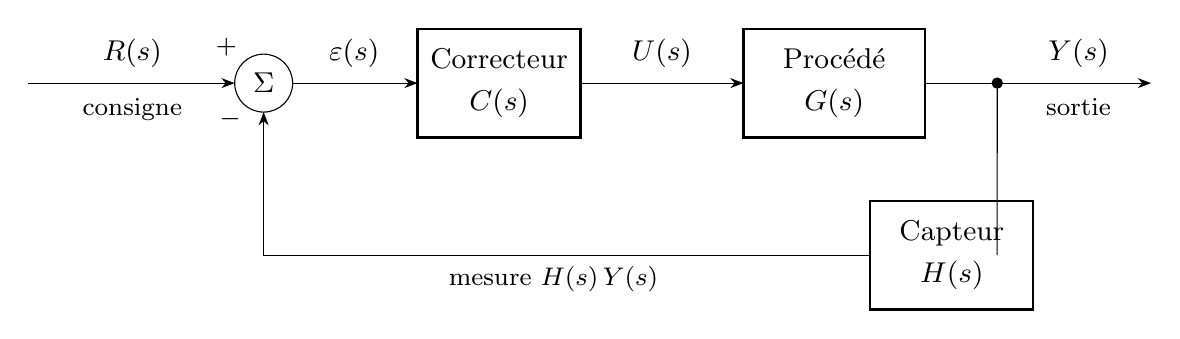
\begin{tikzpicture}[>=Stealth, scale=1.15, every node/.style={font=\small}, transform shape]
  % Sommateur
  \draw (0,0) circle (0.32);
  \node at (0,0) {$\Sigma$};
  \node[above left=-2pt] at (-0.22,0.22) {\footnotesize $+$};
  \node[below left=-2pt] at (-0.18,-0.22) {\footnotesize $-$};
  % Entrée consigne
  \draw[->] (-2.6,0) -- (-0.32,0);
  \node[above] at (-1.45,0.05) {$R(s)$};
  \node[below, font=\footnotesize] at (-1.45,-0.05) {consigne};
  % Erreur
  \draw[->] (0.32,0) -- (1.7,0);
  \node[above] at (1.0,0.05) {$\varepsilon(s)$};
  % Correcteur
  \draw[thick] (1.7,-0.6) rectangle (3.5,0.6);
  \node[align=center] at (2.6,0) {Correcteur\\[2pt] $C(s)$};
  % Commande
  \draw[->] (3.5,0) -- (5.3,0);
  \node[above] at (4.4,0.05) {$U(s)$};
  % Procédé
  \draw[thick] (5.3,-0.6) rectangle (7.3,0.6);
  \node[align=center] at (6.3,0) {Procédé\\[2pt] $G(s)$};
  % Sortie
  \draw[->] (7.3,0) -- (9.8,0);
  \node[above] at (9.0,0.05) {$Y(s)$};
  \node[below, font=\footnotesize] at (9.0,-0.05) {sortie};
  \coordinate (tap) at (8.1,0);
  \filldraw (tap) circle (1.6pt);
  % Retour par le capteur
  \draw (tap) -- (8.1,-1.9);
  \draw[thick] (6.7,-2.5) rectangle (8.5,-1.3);
  \node[align=center] at (7.6,-1.9) {Capteur\\[2pt] $H(s)$};
  \draw[->] (6.7,-1.9) -- (0,-1.9) -- (0,-0.32);
  \node[below, font=\footnotesize] at (3.2,-1.9) {mesure $H(s)\,Y(s)$};
\end{tikzpicture}
\end{center}

\begin{formule}
\begin{itemize}[nosep]
\item \textbf{La consigne} $R(s)$ : la valeur désirée (température voulue, tension de sortie\ldots), exprimée dans le domaine de Laplace.
\item \textbf{Le comparateur} (sommateur) : calcule l'\textbf{erreur} $\varepsilon(s) = R(s) - H(s)Y(s)$.
\item \textbf{Le correcteur} $C(s)$ : transforme l'erreur en commande (le ``cerveau'' --- chapitre 34).
\item \textbf{Le procédé} $G(s)$ : le système à piloter (le moteur, le convertisseur, la pièce à chauffer).
\item \textbf{Le capteur} $H(s)$ : mesure la sortie et la ramène au comparateur.
\end{itemize}
\textbf{Convention :} les blocs sont des \textbf{fonctions de transfert} en $s$ (la transformée de Laplace, introduite dans la section suivante), donc les signaux sont eux aussi notés dans le domaine de Laplace ($R$, $\varepsilon$, $U$, $Y$ en fonction de $s$) --- c'est ce qui rend licite l'écriture ``sortie $=$ bloc $\times$ entrée'' ($Y = G\,U$). En temporel, ce produit serait une convolution.

On reconnaît exactement l'architecture du régulateur de tension (chapitre 30) : référence = consigne, diviseur = capteur, ampli d'erreur = comparateur + correcteur, ballast + charge = procédé. \textbf{Le régulateur était un asservissement qui ne disait pas son nom.}
\end{formule}

\subsection{Pourquoi la contre-réaction est si puissante}

\begin{formule}
Le chapitre 18 l'a montré pour l'AOP ; généralisons. Si le gain direct (correcteur + procédé) est $A$ et le retour est $\beta$, la sortie suit :
\[
\boxed{\frac{y}{r} = \frac{A}{1 + A\beta}}
\]
Quand le \textbf{gain de boucle} $A\beta \gg 1$ :
\[
\frac{y}{r} \approx \frac{1}{\beta}
\]
\textbf{Trois conséquences décisives :}
\begin{enumerate}[nosep]
\item \textbf{Précision} : la sortie ne dépend (presque) plus de $A$, mais seulement du retour $\beta$ --- des composants passifs précis et stables (un diviseur résistif).
\item \textbf{Insensibilité} : si $A$ varie (température, vieillissement, dispersion), $y/r$ bouge très peu --- la boucle ``absorbe'' les imperfections du procédé.
\item \textbf{Rejet de perturbation} : une perturbation entrant dans le procédé est divisée par $1 + A\beta$ en sortie. Plus le gain de boucle est élevé, mieux la boucle ``efface'' les perturbations.
\end{enumerate}
\textbf{C'est tout l'intérêt d'asservir :} échanger du gain (qu'on a en abondance) contre de la précision, de la stabilité et de l'immunité (qu'on désire).
\end{formule}

\begin{retenir}
\textbf{L'essentiel :}
\begin{enumerate}[nosep]
\item Boucle ouverte : aveugle. Boucle fermée : mesure, compare, corrige l'erreur.
\item Éléments : consigne, comparateur, correcteur $C(s)$, procédé $G(s)$, capteur $H(s)$.
\item Contre-réaction : $y/r = A/(1+A\beta) \to 1/\beta$ si $A\beta \gg 1$.
\item On échange du gain contre précision, insensibilité et rejet de perturbation.
\end{enumerate}
\end{retenir}

% ============================================================================
\section{Approfondissement}

\vspace{0.3cm}
\textit{L'outil qui rend tout cela calculable : la transformée de Laplace, les fonctions de transfert, et les pôles qui gouvernent la dynamique.}
\vspace{0.3cm}

\begin{approfondissement}
La transformée de Laplace, la fonction de transfert, pôles et zéros, et les réponses des systèmes du 1\textsuperscript{er} et 2\textsuperscript{nd} ordre. Prérequis : chapitres 9 (RC), 13 (Bode), 14 (fonctions de transfert).
\end{approfondissement}

\subsection{La transformée de Laplace : pourquoi et comment}

\begin{formule}
Les systèmes physiques sont décrits par des \textbf{équations différentielles} (un condensateur : $i = C\,dv/dt$ ; une bobine : $v = L\,di/dt$). Les résoudre directement est pénible. La \textbf{transformée de Laplace} les change en équations \textbf{algébriques} grâce à une propriété magique :
\[
\mathcal{L}\!\left[\frac{df}{dt}\right] = s\,F(s) \qquad \mathcal{L}\!\left[\int f\,dt\right] = \frac{F(s)}{s}
\]
\textbf{Dériver devient multiplier par $s$ ; intégrer devient diviser par $s$.} La variable $s = \sigma + j\omega$ est complexe : sa partie imaginaire $\omega$ est la pulsation (le régime sinusoïdal du chapitre 11 est le cas particulier $s = j\omega$), sa partie réelle $\sigma$ décrit la croissance ou décroissance exponentielle.

Une équation différentielle linéaire devient ainsi une simple fraction en $s$, qu'on manipule avec de l'algèbre.
\end{formule}

\begin{intuition}
\textbf{Laplace généralise Fourier.} Le chapitre 13 analysait les circuits en régime sinusoïdal établi avec $j\omega$ : on y voyait l'amplitude et la phase à chaque fréquence. Laplace ajoute la dimension \textit{transitoire} (le $\sigma$) : non seulement ``comment le système répond à chaque fréquence'', mais aussi ``comment il s'établit dans le temps'' (montée, oscillations, amortissement). C'est l'outil unifié du régime établi \textit{et} du transitoire.
\end{intuition}

\subsection{La fonction de transfert, pôles et zéros}

\begin{formule}
La \textbf{fonction de transfert} $H(s) = Y(s)/X(s)$ caractérise entièrement un système linéaire. C'est une fraction rationnelle :
\[
H(s) = K\,\frac{(s - z_1)(s - z_2)\cdots}{(s - p_1)(s - p_2)\cdots}
\]
\begin{itemize}[nosep]
\item Les \textbf{zéros} $z_i$ (racines du numérateur) : fréquences où la transmission s'annule.
\item Les \textbf{pôles} $p_i$ (racines du dénominateur) : fréquences propres du système --- ils \textbf{gouvernent la dynamique}.
\end{itemize}

\textbf{Le critère de stabilité fondamental :}
\[
\boxed{\text{Système stable} \iff \text{tous les pôles ont une partie réelle négative}}
\]
Un pôle $p = \sigma + j\omega$ correspond à une réponse en $e^{\sigma t}\cos(\omega t)$. Si $\sigma < 0$ : l'oscillation s'amortit (stable). Si $\sigma > 0$ : elle diverge (instable). Si $\sigma = 0$ : oscillation entretenue (marginal). \textbf{La stabilité se lit directement dans la position des pôles dans le plan complexe} --- c'est tout l'enjeu du chapitre 34.
\end{formule}

\subsection{Le système du premier ordre}

\begin{formule}
Le plus simple --- déjà rencontré avec le filtre RC (chapitre 9) :
\[
H(s) = \frac{K}{1 + \tau s}
\]
Un seul pôle réel en $s = -1/\tau$. Réponse à un échelon :
\[
y(t) = K\left(1 - e^{-t/\tau}\right)
\]
\begin{itemize}[nosep]
\item $\tau$ : la \textbf{constante de temps}. À $t = \tau$, la sortie a atteint 63\,\% ; à $t = 3\tau$, 95\,\% ; à $t = 5\tau$, 99\,\%.
\item Pas de dépassement, pas d'oscillation : un premier ordre est \textbf{toujours stable} et monotone.
\end{itemize}
C'est le comportement d'une charge de condensateur, d'une mise en température, d'un moteur en vitesse : la signature universelle du ``une seule réserve d'énergie''.
\end{formule}

\subsection{Le système du second ordre}

\begin{formule}
Deux réserves d'énergie qui s'échangent (L et C, masse et ressort\ldots) donnent un second ordre, décrit par sa forme canonique :
\[
H(s) = \frac{K\,\omega_0^2}{s^2 + 2\zeta\omega_0\,s + \omega_0^2}
\]
\begin{itemize}[nosep]
\item $\omega_0$ : la \textbf{pulsation propre} (rapidité intrinsèque).
\item $\zeta$ (zêta) : le \textbf{coefficient d'amortissement}, qui décide tout :
\end{itemize}
\begin{center}
\renewcommand{\arraystretch}{1.3}
\begin{tabular}{p{3.1cm}p{2.7cm}p{6.0cm}}
\toprule
\textbf{Amortissement} & \textbf{Pôles} & \textbf{Réponse à l'échelon} \\
\midrule
$\zeta > 1$ (sur-amorti) & 2 pôles réels & Lente, sans dépassement \\
$\zeta = 1$ (critique) & 1 pôle double réel & La plus rapide \textit{sans} dépassement \\
$0 < \zeta < 1$ (sous-amorti) & 2 pôles complexes & Rapide mais avec \textbf{dépassement} et oscillations \\
$\zeta = 0$ (non amorti) & 2 pôles imaginaires purs & Oscillation entretenue (instable en pratique) \\
\bottomrule
\end{tabular}
\end{center}
\end{formule}

\begin{intuition}
\textbf{Le compromis rapidité/dépassement en une image.} Un $\zeta$ faible donne un système rapide mais qui ``dépasse'' la cible et oscille avant de se stabiliser (pensez à une suspension de voiture trop souple qui rebondit). Un $\zeta$ élevé ne dépasse jamais mais est lent (suspension trop dure). L'amortissement critique $\zeta = 1$ est la frontière : le plus rapide \textit{sans} dépassement. En pratique on vise souvent $\zeta \approx 0{,}7$ --- un dépassement modéré ($\sim 5\,\%$) pour gagner en rapidité. C'est exactement le réglage d'un correcteur (chapitre 34) et la signature de la résonance LC d'un découpage (chapitre 32).
\end{intuition}

% ============================================================================
\section{Niveau Ingénieur}

\begin{ingenieur}
La précision en régime permanent, le compromis rapidité/stabilité, et la vision unifiée : tout le livre était de l'asservissement. Prérequis : chapitres 18, 30, 32.
\end{ingenieur}

\subsection{La précision : erreur statique et classe du système}

\begin{formule}
Une boucle suit-elle exactement sa consigne en régime établi ? Le \textbf{théorème de la valeur finale} donne l'erreur permanente :
\[
\varepsilon_\infty = \lim_{t\to\infty}\varepsilon(t) = \lim_{s\to 0} s\,\varepsilon(s)
\]
Le résultat dépend du nombre d'\textbf{intégrateurs} (pôles en $s = 0$) dans la boucle ouverte --- la \textbf{classe} du système :
\begin{itemize}[nosep]
\item \textbf{Classe 0} (aucun intégrateur) : erreur statique \textbf{non nulle} sur une consigne constante. Elle vaut $1/(1 + K)$ : plus le gain $K$ est grand, plus l'erreur est faible, mais jamais nulle.
\item \textbf{Classe 1} (un intégrateur) : erreur statique \textbf{nulle} sur une consigne constante (l'intégrateur accumule l'erreur jusqu'à l'annuler), mais erreur constante sur une rampe.
\item \textbf{Classe 2} (deux intégrateurs) : suit même les rampes sans erreur.
\end{itemize}
\textbf{C'est pourquoi un correcteur intégral (le ``I'' du PID, chapitre 34) est si précieux} : il ajoute un intégrateur, donc annule l'erreur statique. Le régulateur de tension du chapitre 30 atteint sa précision exactement ainsi --- son ampli d'erreur à fort gain agit comme un quasi-intégrateur.
\end{formule}

\subsection{Le compromis fondamental : rapidité contre stabilité}

\begin{attention}
\textbf{On ne peut pas être à la fois infiniment rapide et infiniment stable.} Augmenter le gain de boucle (pour la précision et la rapidité) rapproche les pôles de l'axe imaginaire, voire les fait passer à droite : le système devient oscillant, puis instable. C'est le même mur qu'au chapitre 18 (marges de phase) et au chapitre 32 (stabilité du SMPS), vu maintenant côté pôles :
\begin{itemize}[nosep]
\item Gain trop \textbf{faible} : stable mais lent et imprécis (erreur statique élevée).
\item Gain trop \textbf{fort} : rapide mais oscillant, dépassement excessif, voire instabilité.
\item \textbf{Le bon réglage} : assez de gain pour la précision et la rapidité, pas trop pour garder une marge de stabilité ($\zeta \approx 0{,}7$, marge de phase $\sim\SI{60}{°}$).
\end{itemize}
Concevoir un correcteur (chapitre 34), c'est naviguer ce compromis : placer les pôles de la boucle fermée là où l'on veut, entre rapidité et amortissement.
\end{attention}

\subsection{Perturbations et robustesse}

\begin{formule}
Un bon asservissement ne suit pas seulement la consigne : il \textbf{rejette les perturbations}. Une perturbation $d(s)$ entrant dans le procédé apparaît en sortie atténuée par le gain de boucle :
\[
\frac{y}{d} = \frac{G}{1 + C\,G\,H}
\]
Plus $|CGH|$ est grand \textbf{dans la bande de la perturbation}, mieux elle est rejetée. Mais ce gain chute avec la fréquence (pôles) : une boucle rejette bien les perturbations \textbf{lentes} (dérive thermique, variation de charge moyenne) et mal les \textbf{rapides} (au-delà de sa bande passante). C'est exactement ce qu'on a vu au chapitre 30 : le PSRR d'un régulateur, excellent en continu, s'effondre en haute fréquence --- le PSRR \textit{est} le rejet de perturbation de la boucle d'alimentation.
\end{formule}

\subsection{Vision unifiée : tout le livre était de l'asservissement}

\begin{intuition}
\textbf{Ce chapitre révèle la structure cachée de la moitié du livre.}
\begin{itemize}[nosep]
\item L'\textbf{AOP contre-réactionné} (chapitre 18) : $y/r = A/(1+A\beta)$, gain de boucle, marges de phase --- c'était un asservissement de tension.
\item Le \textbf{régulateur linéaire} (chapitre 30) : référence, capteur, ampli d'erreur, ballast --- un asservissement, précis grâce à son quasi-intégrateur.
\item L'\textbf{alimentation à découpage} (chapitre 32) : pôle LC, compensation Type III, mode courant --- un asservissement avec un procédé du second ordre.
\item Le \textbf{sigma-delta} (chapitre 27), la \textbf{PLL} (chapitre 22), la \textbf{polarisation} d'un transistor (chapitre 16) : tous des boucles.
\end{itemize}
La transformée de Laplace et l'analyse des pôles sont le langage commun de tous ces systèmes. Le chapitre 34 complète l'outillage : le correcteur PID, le lieu des racines, et la lecture des marges sur Bode --- de quoi \textbf{concevoir} n'importe quel asservissement, et non plus seulement le reconnaître.
\end{intuition}

% === EXERCICES ===
\section*{Exercices}
\addcontentsline{toc}{section}{Exercices}

\subsection*{Niveau débutant}

\textbf{Exercice 33.1 ---} Un système du premier ordre a $\tau = \SI{200}{ms}$. (a) Combien de temps pour atteindre 95\,\% de la valeur finale ? (b) 99\,\% ? (c) Y a-t-il un dépassement ?

\begin{pratique}
\textbf{Solution :}

(a) 95\,\% à $t = 3\tau = \SI{600}{ms}$. \quad (b) 99\,\% à $t = 5\tau = \SI{1}{s}$.

(c) Non : un premier ordre n'a qu'un pôle réel, sa réponse est monotone croissante --- jamais de dépassement ni d'oscillation. Le dépassement exige au moins un second ordre sous-amorti.
\end{pratique}

\textbf{Exercice 33.2 ---} Un asservissement a un gain direct $A = 1000$ et un retour $\beta = 0{,}1$. (a) Quel est le gain en boucle fermée $y/r$ ? (b) Si $A$ chute à 500 (vieillissement), de combien varie $y/r$ ?

\begin{pratique}
\textbf{Solution :}

(a) $y/r = A/(1+A\beta) = 1000/(1+100) = 1000/101 = 9{,}90$.

(b) $A = 500$ : $y/r = 500/(1+50) = 500/51 = 9{,}80$. Variation : $(9{,}90-9{,}80)/9{,}90 = 1\,\%$ pour une chute de \textbf{50\,\%} de $A$. La boucle a divisé la sensibilité par $\sim 50$ (le facteur $1+A\beta$) : c'est l'insensibilité de la contre-réaction en action.
\end{pratique}

\subsection*{Niveau intermédiaire}

\textbf{Exercice 33.3 ---} Un système du second ordre a $\omega_0 = \SI{100}{rad/s}$ et $\zeta = 0{,}5$. (a) Les pôles sont-ils réels ou complexes ? (b) Calculez-les. (c) Le système est-il stable ?

\begin{pratique}
\textbf{Solution :} pôles racines de $s^2 + 2\zeta\omega_0 s + \omega_0^2 = 0$, soit $s = -\zeta\omega_0 \pm \omega_0\sqrt{\zeta^2-1}$.

(a) $\zeta = 0{,}5 < 1 \Rightarrow$ racine négative sous le radical $\Rightarrow$ pôles \textbf{complexes conjugués}.

(b) $s = -0{,}5\times100 \pm 100\sqrt{0{,}25-1} = -50 \pm 100\,j\sqrt{0{,}75} = -50 \pm 86{,}6\,j$.

(c) Partie réelle $= -50 < 0$ pour les deux pôles $\Rightarrow$ \textbf{stable}. La réponse oscille à $\sim\SI{86.6}{rad/s}$ en s'amortissant avec une enveloppe en $e^{-50t}$. Comme $\zeta < 1$, il y aura du dépassement.
\end{pratique}

\textbf{Exercice 33.4 ---} On applique un échelon à un circuit RLC série ($R = \SI{10}{\ohm}$, $L = \SI{1}{mH}$, $C = \SI{1}{\micro F}$), sortie aux bornes de $C$. (a) Calculez $\omega_0$ et $\zeta$. (b) Le régime est-il oscillant ?

\begin{pratique}
\textbf{Solution :} pour un RLC série, $\omega_0 = 1/\sqrt{LC}$ et $\zeta = \frac{R}{2}\sqrt{C/L}$.

(a) $\omega_0 = 1/\sqrt{10^{-3}\times10^{-6}} = 1/\sqrt{10^{-9}} = \SI{31623}{rad/s}$ ($\approx \SI{5.03}{kHz}$).

$\zeta = \frac{10}{2}\sqrt{10^{-6}/10^{-3}} = 5\times\sqrt{10^{-3}} = 5\times0{,}0316 = 0{,}158$.

(b) $\zeta = 0{,}158 \ll 1$ : régime \textbf{très oscillant} (faiblement amorti), avec un dépassement important. C'est le même second ordre que le filtre LC de sortie d'un découpage (chapitre 32) --- d'où la nécessité d'amortir ou de compenser.
\end{pratique}

\subsection*{Niveau ingénieur}

\textbf{Exercice 33.5 ---} Une boucle de classe 0 a un gain de boucle statique $K = 49$. (a) Quelle erreur statique sur une consigne constante ? (b) Que devient-elle si on ajoute un intégrateur (classe 1) ? (c) Quel inconvénient l'intégrateur introduit-il ?

\begin{pratique}
\textbf{Solution :}

(a) Erreur statique classe 0 : $\varepsilon_\infty = 1/(1+K) = 1/50 = 2\,\%$. La sortie se stabilise 2\,\% en dessous de la consigne, indéfiniment.

(b) Avec un intégrateur (classe 1) : $\varepsilon_\infty = 0$. L'intégrateur accumule l'erreur tant qu'elle est non nulle, jusqu'à l'annuler complètement. C'est la précision parfaite en régime établi.

(c) L'intégrateur ajoute $-\SI{90}{°}$ de phase à toutes les fréquences $\Rightarrow$ il \textbf{dégrade la marge de phase} et tend à déstabiliser. Tout l'art du correcteur PID (chapitre 34) est de bénéficier de la précision du ``I'' sans perdre la stabilité --- d'où l'ajout du terme dérivé ``D''.
\end{pratique}

\textbf{Exercice 33.6 ---} Un régulateur de tension (chapitre 30) a un gain de boucle de \SI{80}{dB} en continu, tombant à \SI{20}{dB} à \SI{100}{kHz}. (a) De combien atténue-t-il une perturbation d'alimentation à \SI{100}{Hz} (gain de boucle $\approx \SI{80}{dB}$) ? (b) À \SI{100}{kHz} ? (c) Reliez au PSRR du chapitre 30.

\begin{pratique}
\textbf{Solution :} le rejet de perturbation vaut $\approx 1+|CGH| \approx |CGH|$ quand le gain est grand.

(a) À \SI{100}{Hz} : \SI{80}{dB} de gain de boucle $\Rightarrow$ atténuation $\times 10^{80/20} = \times 10\,000$. Une ondulation de \SI{100}{mV} devient \SI{10}{\micro V}. Excellent.

(b) À \SI{100}{kHz} : \SI{20}{dB} $\Rightarrow$ atténuation $\times 10 = $ seulement. Une ondulation de \SI{100}{mV} devient \SI{10}{mV}. Médiocre.

(c) C'est exactement le PSRR : il \textit{est} le gain de boucle de l'alimentation vu comme rejet de perturbation. Fort en continu, faible en HF --- d'où l'inefficacité d'un LDO seul contre l'ondulation de découpage (chapitre 30), et la nécessité d'un filtrage LC complémentaire.
\end{pratique}

\subsection*{Questions de compréhension}

\begin{enumerate}[nosep]
\item En quoi une commande en boucle fermée est-elle fondamentalement supérieure à une boucle ouverte face aux perturbations et aux erreurs de modèle ? Donnez l'intuition, pas la formule.
\item La transformée de Laplace change la dérivation en multiplication par $s$. Pourquoi cette simple propriété rend-elle les équations différentielles solubles par algèbre ?
\item Pourquoi la stabilité se lit-elle dans le signe de la partie réelle des pôles ? Reliez un pôle $\sigma + j\omega$ à une réponse temporelle $e^{\sigma t}\cos(\omega t)$.
\item Un intégrateur annule l'erreur statique mais dégrade la stabilité. Expliquez ce double effet et pourquoi il motive l'ajout d'un terme dérivé dans un PID.
\end{enumerate}

% === RÉSUMÉ ===
\section*{Résumé du chapitre}
\addcontentsline{toc}{section}{Résumé du chapitre}

\begin{bases}[title={\color{white} Résumé --- Les Bases}]
\begin{center}
\renewcommand{\arraystretch}{1.3}
\begin{tabular}{p{3.5cm}p{9.5cm}}
\toprule
Boucle ouverte/fermée & Ouverte : aveugle. Fermée : mesure, compare, corrige l'erreur \\
Éléments & Consigne, comparateur, correcteur $C(s)$, procédé $G(s)$, capteur $H(s)$ \\
Contre-réaction & $y/r = A/(1+A\beta) \to 1/\beta$ si $A\beta \gg 1$ \\
Intérêt & Précision + insensibilité + rejet de perturbation (gain échangé contre qualité) \\
\bottomrule
\end{tabular}
\end{center}
\end{bases}

\begin{approfondissement}[title={\color{white} Résumé --- Approfondissement}]
\begin{center}
\renewcommand{\arraystretch}{1.3}
\begin{tabular}{p{3.5cm}p{9.5cm}}
\toprule
Laplace & Dériver $\to \times s$, intégrer $\to /s$ : équations diff. deviennent algèbre \\
Fonction de transfert & $H(s) = Y/X$, fraction rationnelle. Pôles gouvernent la dynamique \\
Stabilité & Stable $\iff$ tous les pôles à partie réelle négative \\
1\textsuperscript{er} ordre & $K/(1+\tau s)$ : monotone, 63\,\% à $\tau$, toujours stable \\
2\textsuperscript{nd} ordre & $\omega_0$, $\zeta$ : $\zeta<1$ oscillant, $\zeta=1$ critique, $\zeta\approx0{,}7$ optimal \\
\bottomrule
\end{tabular}
\end{center}
\end{approfondissement}

\begin{ingenieur}[title={\color{white} Résumé --- Niveau Ingénieur}]
\begin{center}
\renewcommand{\arraystretch}{1.3}
\begin{tabular}{p{3.5cm}p{9.5cm}}
\toprule
Précision & Classe (nb d'intégrateurs) : classe 0 erreur $1/(1+K)$, classe 1 erreur nulle \\
Compromis & Rapidité vs stabilité : gain $\uparrow$ rapproche les pôles de l'instabilité \\
Rejet perturbation & $y/d = G/(1+CGH)$ : fort en BF, faible en HF (= le PSRR du Ch.30) \\
Vision unifiée & AOP, régulateur, SMPS, PLL, sigma-delta : tous des asservissements \\
\bottomrule
\end{tabular}
\end{center}
\end{ingenieur}

% ============================================================================
% CHAPITRE 34 : CORRECTEUR PID, LIEU DES RACINES ET MARGES DE STABILITÉ
% VERSION PEER-REVIEW
% Fichier autonome à intégrer dans Bible_Elec.tex
% Clôt la PARTIE VIII : ASSERVISSEMENT
% ============================================================================

\chapter{Correcteur PID, lieu des racines et marges de stabilité}

\begin{center}
\textit{Le chapitre précédent a posé le cadre : une boucle, un procédé, un correcteur.\\
Restait la question décisive --- comment régler ce correcteur ?\\
Trois actions suffisent à dompter presque tous les systèmes :\\
proportionnelle, intégrale, dérivée. Ce chapitre montre ce que fait\\
chacune, comment placer les pôles de la boucle fermée (lieu des racines),\\
et comment lire la stabilité directement sur Bode.}
\end{center}

\vspace{0.5cm}

Le chapitre 33 a formalisé l'asservissement et introduit Laplace ; il restait le correcteur $C(s)$ comme une boîte à remplir. Ce chapitre la remplit avec le \textbf{PID}, le correcteur universel de l'industrie : trois actions élémentaires --- \textbf{P}roportionnelle, \textbf{I}ntégrale, \textbf{D}érivée --- dont la combinaison règle le compromis précision / rapidité / stabilité. On verra ensuite deux outils de conception complémentaires : le \textbf{lieu des racines} (où vont les pôles quand on monte le gain) et la lecture des \textbf{marges} sur Bode (chapitre 18). C'est le chapitre qui transforme la compréhension des boucles en capacité à les \textit{concevoir}.

% ============================================================================
\section{Les Bases}

\begin{bases}
Les trois actions du PID --- ce que chacune fait, son intérêt et son défaut. Prérequis : chapitre 33 (boucle fermée, erreur, classe), chapitre 18 (rétroaction).
\end{bases}

\subsection{L'action proportionnelle (P) : réagir à l'erreur}

\begin{formule}
La commande est proportionnelle à l'erreur :
\[
u = K_p\,\varepsilon
\]
Plus l'écart est grand, plus on corrige fort. C'est l'instinct de base : « loin de la cible $\Rightarrow$ pousser fort ; proche $\Rightarrow$ pousser doucement ».

\textbf{Effets de $K_p$ :}
\begin{itemize}[nosep]
\item $K_p \uparrow$ : réponse plus \textbf{rapide} et erreur statique \textbf{réduite} (mais jamais nulle en classe 0, chapitre 33 : $\varepsilon_\infty = 1/(1+K)$).
\item $K_p$ trop grand : la boucle \textbf{oscille}, puis devient instable (les pôles se rapprochent de l'axe imaginaire).
\end{itemize}
\textbf{Le défaut intrinsèque du P seul : l'erreur résiduelle.} Pour produire une commande, il faut une erreur non nulle ($u = K_p\varepsilon$ : si $\varepsilon = 0$, $u = 0$). Un correcteur purement proportionnel laisse donc toujours un écart permanent --- il faut le terme intégral pour l'effacer.
\end{formule}

\subsection{L'action intégrale (I) : effacer l'erreur résiduelle}

\begin{formule}
La commande intègre l'erreur dans le temps :
\[
u = K_i \int \varepsilon\,dt
\]
Tant qu'il reste une erreur, l'intégrale \textbf{s'accumule} et pousse la commande --- jusqu'à ce que l'erreur soit \textbf{exactement nulle}. C'est l'intégrateur de la classe 1 (chapitre 33) qui annule l'erreur statique.

\textbf{Effets de $K_i$ :}
\begin{itemize}[nosep]
\item \textbf{Erreur statique nulle} : l'avantage décisif. La sortie atteint exactement la consigne en régime établi.
\item \textbf{Mais $-\SI{90}{°}$ de phase} ajoutés (un intégrateur, chapitre 33) : l'intégrale \textbf{dégrade la stabilité} et ralentit la réponse. Trop d'intégrale $\Rightarrow$ oscillations lentes.
\end{itemize}
\end{formule}

\subsection{L'action dérivée (D) : anticiper}

\begin{formule}
La commande réagit à la \textbf{vitesse} de variation de l'erreur :
\[
u = K_d\,\frac{d\varepsilon}{dt}
\]
Si l'erreur diminue vite, le dérivé \textbf{freine} la commande à l'avance, avant d'atteindre la cible : il \textbf{anticipe} et amortit. C'est le terme qui ajoute de l'amortissement et réduit le dépassement.

\textbf{Effets de $K_d$ :}
\begin{itemize}[nosep]
\item $+\SI{90}{°}$ de phase (un dérivateur) : il \textbf{améliore la marge de phase} et la stabilité, autorise un $K_p$ plus élevé donc une réponse plus rapide sans osciller.
\item \textbf{Mais il amplifie le bruit} : dériver un signal bruité (chapitre 18, $e_n$) accentue les hautes fréquences. Un dérivé pur est inutilisable tel quel --- il faut le filtrer (niveau ingénieur).
\end{itemize}
\end{formule}

\begin{intuition}
\textbf{Conduire une voiture résume le PID.} Le \textbf{P} regarde l'écart actuel à la ligne (corriger proportionnellement). Le \textbf{I} corrige un défaut persistant (volant légèrement décentré $\Rightarrow$ on accumule une correction jusqu'à rouler droit). Le \textbf{D} anticipe : voyant le virage \textit{arriver}, on tourne \textit{avant} de dévier. P réagit au présent, I corrige le passé accumulé, D anticipe le futur.
\end{intuition}

\begin{retenir}
\textbf{L'essentiel :}
\begin{enumerate}[nosep]
\item \textbf{P} ($K_p\varepsilon$) : rapidité, réduit l'erreur sans l'annuler. Trop $\Rightarrow$ oscille.
\item \textbf{I} ($K_i\!\int\!\varepsilon$) : annule l'erreur statique, mais $-\SI{90}{°}$ de phase $\Rightarrow$ déstabilise.
\item \textbf{D} ($K_d\,d\varepsilon/dt$) : anticipe, amortit, $+\SI{90}{°}$ de phase, mais amplifie le bruit.
\item Le PID combine les trois : précision (I) + rapidité (P) + amortissement (D).
\end{enumerate}
\end{retenir}

% ============================================================================
\section{Approfondissement}

\vspace{0.3cm}
\textit{Le PID complet, l'effet de chaque action sur la réponse, et le réglage du correcteur.}
\vspace{0.3cm}

\begin{approfondissement}
La fonction de transfert du PID, l'effet des termes sur la réponse indicielle, et les méthodes de réglage. Prérequis : chapitres 13 (Bode), 33 (Laplace, pôles).
\end{approfondissement}

\subsection{La fonction de transfert du PID}

\begin{formule}
En combinant les trois actions et en passant en Laplace (chapitre 33) :
\[
\boxed{C(s) = K_p + \frac{K_i}{s} + K_d\,s = K_p\left(1 + \frac{1}{T_i\,s} + T_d\,s\right)}
\]
\begin{itemize}[nosep]
\item $T_i = K_p/K_i$ : la \textbf{constante de temps d'intégration} (temps pour que l'action I égale l'action P).
\item $T_d = K_d/K_p$ : la \textbf{constante de temps de dérivation} (horizon d'anticipation).
\end{itemize}
Le PID apporte un \textbf{pôle à l'origine} (l'intégrateur, en $s = 0$) et \textbf{deux zéros} (réglables via $T_i$, $T_d$). Ces deux zéros sont les leviers du concepteur : on les place pour ``rattraper'' la phase que les pôles du procédé font chuter --- c'est précisément le rôle des compensateurs Type II/III du découpage (chapitre 32), qui sont des PID déguisés.
\end{formule}

\subsection{L'effet de chaque action sur la réponse indicielle}

\begin{center}
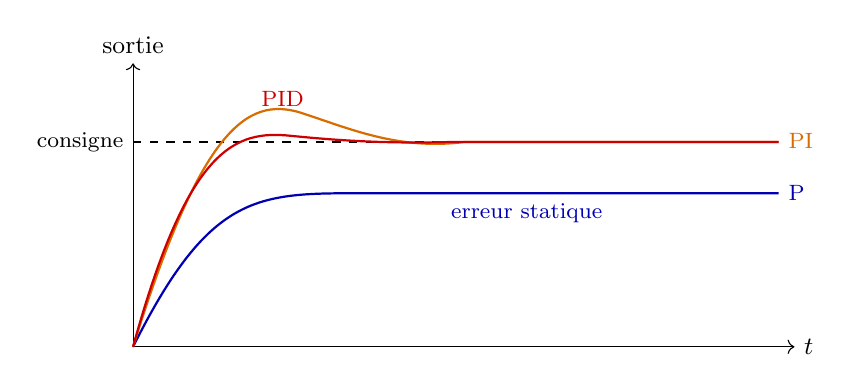
\begin{tikzpicture}[scale=1.0]
  % Axes
  \draw[->] (0,0) -- (8.4,0) node[right, font=\small]{$t$};
  \draw[->] (0,0) -- (0,3.6) node[above, font=\small]{sortie};
  % Consigne
  \draw[dashed, thick] (0,2.6) -- (8.2,2.6);
  \node[left, font=\footnotesize] at (0,2.6) {consigne};
  % P seul : monte et se stabilise sous la consigne (erreur statique)
  \draw[thick, blue!70!black] (0,0) .. controls (1.0,2.0) and (1.6,1.95) .. (3.0,1.95) -- (8.2,1.95);
  \node[blue!70!black, font=\footnotesize, right] at (8.2,1.95) {P};
  \node[blue!70!black, font=\footnotesize] at (5.0,1.7) {erreur statique};
  % PI : monte, dépasse, revient sur la consigne
  \draw[thick, orange!85!black] (0,0) .. controls (0.9,2.9) and (1.5,3.2) .. (2.2,2.95) .. controls (2.8,2.75) and (3.4,2.5) .. (4.2,2.6) -- (8.2,2.6);
  \node[orange!85!black, font=\footnotesize, right] at (8.2,2.62) {PI};
  % PID : monte vite, peu de dépassement, sur la consigne
  \draw[thick, red!80!black] (0,0) .. controls (0.7,2.55) and (1.3,2.75) .. (2.0,2.68) .. controls (2.6,2.62) and (3.2,2.58) .. (4.0,2.6) -- (8.2,2.6);
  \node[red!80!black, font=\footnotesize] at (1.9,3.15) {PID};
\end{tikzpicture}
\end{center}

\begin{formule}
\textbf{Lecture du graphe :}
\begin{itemize}[nosep]
\item \textbf{P seul} (bleu) : réponse rapide mais se stabilise \textit{sous} la consigne --- l'erreur statique résiduelle.
\item \textbf{PI} (orange) : l'intégrale efface l'erreur (la courbe rejoint la consigne) mais au prix d'un \textbf{dépassement} et d'oscillations (le $-\SI{90}{°}$ de l'intégrateur).
\item \textbf{PID} (rouge) : le terme dérivé amortit $\Rightarrow$ montée rapide, dépassement réduit, et toujours erreur nulle. Le meilleur compromis.
\end{itemize}
\end{formule}

\begin{pratique}
\textbf{Effet qualitatif d'une augmentation de chaque gain (toutes choses égales) :}
\begin{center}
\renewcommand{\arraystretch}{1.35}
\begin{tabular}{p{1.8cm}p{2.2cm}p{2.3cm}p{2.2cm}p{2.0cm}}
\toprule
\textbf{Gain} & \textbf{Rapidité} & \textbf{Dépass.} & \textbf{Err. stat.} & \textbf{Stabilité} \\
\midrule
$K_p \uparrow$ & augmente & augmente & diminue & dégrade \\
$K_i \uparrow$ & augmente & augmente & \textbf{annule} & dégrade \\
$K_d \uparrow$ & ~$\approx$ & diminue & ~$\approx$ & améliore \\
\bottomrule
\end{tabular}
\end{center}
Ce tableau guide le réglage manuel : on augmente $K_p$ pour la rapidité, on ajoute $K_i$ pour la précision, on dose $K_d$ pour amortir le dépassement qu'ils créent.
\end{pratique}

\subsection{Régler un PID : les méthodes}

\begin{formule}
\textbf{Réglage manuel} (le plus courant en pratique) : augmenter $K_p$ jusqu'à une réponse vive mais limite-oscillante, ajouter $K_i$ pour annuler l'erreur statique, puis $K_d$ pour réduire le dépassement. Itérer.

\textbf{Méthode de Ziegler-Nichols} (réglage empirique classique) : on augmente $K_p$ (sans I ni D) jusqu'au \textbf{gain critique} $K_u$ où la boucle oscille de façon entretenue, à la \textbf{période} $T_u$. Des formules empiriques donnent alors $K_p$, $T_i$, $T_d$ à partir de $K_u$ et $T_u$. Rapide mais agressif (dépassement marqué) : un point de départ, pas un réglage final.

\textbf{Réglage par modèle} : si l'on connaît $G(s)$, on place les pôles de la boucle fermée à la position désirée (lieu des racines, niveau ingénieur) ou l'on impose une marge de phase cible sur Bode. C'est l'approche de conception, par opposition à l'empirique.
\end{formule}

% ============================================================================
\section{Niveau Ingénieur}

\begin{ingenieur}
Le lieu des racines, les marges de stabilité sur Bode, et le PID réel (filtrage du dérivé, anti-windup, version numérique). Prérequis : chapitres 13 (Bode), 18 (marges), 33 (pôles).
\end{ingenieur}

\subsection{Le lieu des racines : où vont les pôles}

\begin{formule}
Le \textbf{lieu des racines} (\textit{root locus}) trace le déplacement des \textbf{pôles de la boucle fermée} dans le plan complexe quand on fait varier un paramètre --- typiquement le gain $K$ --- de 0 à l'infini.
\end{formule}

\begin{center}
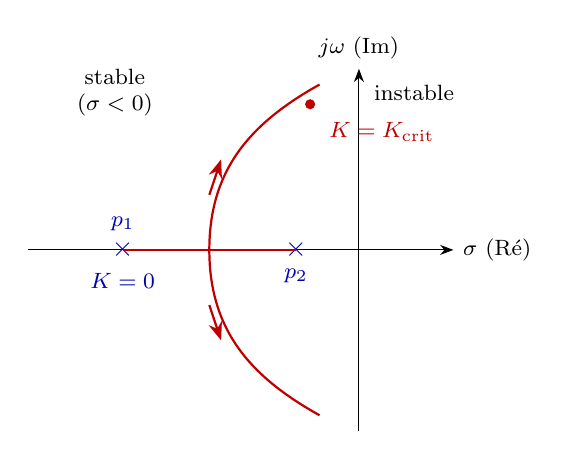
\begin{tikzpicture}[scale=1.0, >=Stealth]
  % Axes (plan complexe)
  \draw[->] (-4.2,0) -- (1.2,0) node[right, font=\footnotesize]{$\sigma$ (Ré)};
  \draw[->] (0,-2.3) -- (0,2.3) node[above, font=\footnotesize]{$j\omega$ (Im)};
  % Axe imaginaire = frontière de stabilité
  \node[font=\footnotesize, align=center] at (-3.1,2.0) {stable\\ ($\sigma<0$)};
  \node[font=\footnotesize, align=center] at (0.7,2.0) {instable};
  % Pôles en boucle ouverte (croix)
  \node at (-3.0,0) {\textcolor{blue!70!black}{$\times$}};
  \node at (-0.8,0) {\textcolor{blue!70!black}{$\times$}};
  \node[above, font=\footnotesize, blue!70!black] at (-3.0,0.12) {$p_1$};
  \node[below, font=\footnotesize, blue!70!black] at (-0.8,-0.12) {$p_2$};
  % Branches : partent des pôles, se rejoignent puis montent vers l'axe imaginaire
  % Branche le long de l'axe réel entre les deux pôles
  \draw[thick, red!75!black] (-3.0,0) -- (-1.9,0);
  \draw[thick, red!75!black] (-0.8,0) -- (-1.9,0);
  % Point de séparation puis branches complexes qui montent et traversent l'axe imaginaire
  \draw[thick, red!75!black] (-1.9,0) .. controls (-1.9,1.0) and (-1.4,1.6) .. (-0.5,2.1);
  \draw[thick, red!75!black] (-1.9,0) .. controls (-1.9,-1.0) and (-1.4,-1.6) .. (-0.5,-2.1);
  % Sens de parcours (K croissant)
  \draw[->, red!75!black, thick] (-1.9,0.7) -- (-1.75,1.15);
  \draw[->, red!75!black, thick] (-1.9,-0.7) -- (-1.75,-1.15);
  % Point de croisement de l'axe imaginaire = limite de stabilité
  \filldraw[red!75!black] (-0.62,1.85) circle (1.6pt);
  \node[right, font=\footnotesize, red!75!black] at (-0.5,1.5) {$K = K_{\text{crit}}$};
  % Légende K=0 sous l'axe, décalée pour ne pas toucher p1
  \node[below, font=\footnotesize, blue!70!black] at (-3.0,-0.18) {$K=0$};
\end{tikzpicture}
\end{center}

\begin{formule}
\textbf{Règles de lecture :}
\begin{itemize}[nosep]
\item Les branches \textbf{partent des pôles} de la boucle ouverte ($K = 0$, croix bleues) et finissent sur les zéros ou à l'infini ($K \to \infty$).
\item Quand $K$ augmente, les pôles se déplacent : ici ils se rejoignent sur l'axe réel, puis \textbf{partent en complexes} (le système devient oscillant) et \textbf{montent vers l'axe imaginaire}.
\item \textbf{Le point de croisement de l'axe imaginaire donne le gain critique $K_{\text{crit}}$ :} au-delà, les pôles passent dans le demi-plan droit ($\sigma > 0$) $\Rightarrow$ \textbf{instabilité} (chapitre 33).
\end{itemize}
\textbf{L'intérêt pour le concepteur :} le lieu des racines montre d'un coup d'œil jusqu'où l'on peut pousser le gain, et où placer les zéros du correcteur (PID) pour ``tirer'' les branches vers la gauche (plus de stabilité) ou les amortir. Ajouter un zéro attire le lieu vers lui --- c'est ainsi que le terme dérivé stabilise.
\end{formule}

\subsection{Les marges de stabilité sur Bode}

\begin{formule}
La même information se lit sur le diagramme de Bode du \textbf{gain de boucle} $T(s) = C(s)G(s)H(s)$ (chapitres 13, 18), souvent plus pratique en conception fréquentielle :
\end{formule}

\begin{center}
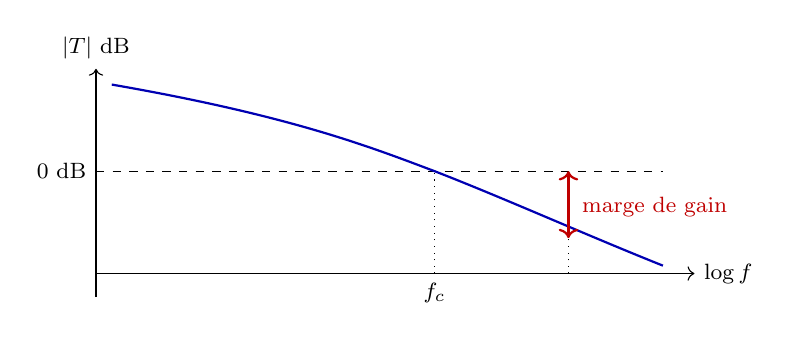
\begin{tikzpicture}[scale=1.0]
  % --- Diagramme de gain ---
  \draw[->] (0,0) -- (7.6,0) node[right, font=\footnotesize]{$\log f$};
  \draw[->] (0,-0.3) -- (0,2.6) node[above, font=\footnotesize]{$|T|$ dB};
  \draw[dashed] (0,1.3) -- (7.2,1.3);
  \node[left, font=\footnotesize] at (0,1.3) {0 dB};
  % Courbe de gain décroissante
  \draw[thick, blue!70!black] (0.2,2.4) .. controls (2.5,2.0) and (3.5,1.6) .. (4.3,1.3) .. controls (5.2,0.95) and (6.2,0.5) .. (7.2,0.1);
  % Fréquence de croisement de gain (|T|=1 -> 0dB)
  \draw[dotted] (4.3,0) -- (4.3,1.3);
  \node[below, font=\footnotesize] at (4.3,0) {$f_c$};
  % --- Marge de gain : repère où la phase = -180 ---
  \draw[dotted] (6.0,0) -- (6.0,1.3);
  \draw[<->, red!75!black, thick] (6.0,0.45) -- (6.0,1.3);
  \node[right, font=\footnotesize, red!75!black] at (6.05,0.85) {marge de gain};
\end{tikzpicture}
\end{center}

\begin{formule}
\textbf{Les deux marges (chapitre 18, formalisées) :}
\begin{itemize}[nosep]
\item \textbf{Marge de phase} : à la fréquence de croisement $f_c$ (où $|T| = \SI{0}{dB}$), c'est l'écart entre la phase réelle et $-\SI{180}{°}$. Une marge $> \SI{45}{°}$ (idéalement \SI{60}{°}) garantit un amortissement correct ($\zeta \approx 0{,}7$, chapitre 33).
\item \textbf{Marge de gain} : à la fréquence où la phase atteint $-\SI{180}{°}$, c'est l'écart en dB entre $|T|$ et \SI{0}{dB}. Une marge $> \SI{6}{dB}$ ($\times 2$) donne une réserve avant l'instabilité.
\end{itemize}
\textbf{Le lien entre les deux représentations :} le point où le lieu des racines croise l'axe imaginaire (gain critique) correspond exactement au point où la marge de gain s'annule sur Bode. Ce sont deux vues du \textbf{même} critère de stabilité --- lieu des racines (côté pôles, plan $s$) et marges (côté fréquence, Bode).
\end{formule}

\subsection{Le PID réel : filtrage, anti-windup, numérique}

\begin{attention}
\textbf{Trois corrections indispensables pour un PID utilisable :}

\textbf{1. Filtrage du dérivé.} Un dérivé pur $K_d\,s$ a un gain qui croît \textit{indéfiniment} avec la fréquence : il amplifie le bruit jusqu'à saturer la commande. On utilise donc un \textbf{dérivé filtré} :
\[
K_d\,\frac{s}{1 + \tau_f\,s} \qquad (\tau_f \approx T_d/N,\; N \sim 8\text{--}20)
\]
Le filtre coupe le gain au-delà de $1/\tau_f$ : on garde l'anticipation utile, on jette le bruit HF.

\textbf{2. Anti-windup.} Si l'actionneur \textbf{sature} (un moteur ne dépasse pas sa tension max), l'erreur persiste mais la commande ne peut plus monter --- pourtant l'\textbf{intégrale continue d'accumuler} (\textit{windup}). Au retour dans la zone linéaire, cette intégrale gonflée provoque un énorme dépassement. La parade (\textbf{anti-windup}) : geler ou décharger l'intégrateur tant que la commande est saturée. Indispensable dès qu'il y a saturation --- c'est-à-dire presque toujours.

\textbf{3. Version numérique.} Un PID est aujourd'hui presque toujours implanté dans un microcontrôleur (chapitre 26) : l'intégrale devient une somme, le dérivé une différence, le tout exécuté à la \textbf{période d'échantillonnage} $T_e$. Il faut $T_e$ assez petit devant la dynamique du procédé (typiquement $T_e < T_{\text{réponse}}/10$) pour que la discrétisation (chapitre 27) ne dégrade pas la boucle, et veiller au retard d'échantillonnage qui \textit{réduit} la marge de phase.
\end{attention}

\subsection{Vue d'ensemble : concevoir une boucle, de bout en bout}

\begin{intuition}
\textbf{La démarche complète du concepteur d'asservissement} rassemble tout le livre :
\begin{enumerate}[nosep]
\item \textbf{Modéliser le procédé} $G(s)$ : identifier ses pôles (constantes de temps, résonances --- chapitre 33). Un moteur, un convertisseur (chapitre 32), un étage thermique.
\item \textbf{Choisir la structure du correcteur} : P, PI, ou PID selon le besoin de précision et d'amortissement.
\item \textbf{Régler les gains} : placer les pôles de la boucle fermée (lieu des racines) ou viser une marge de phase de \SI{60}{°} sur Bode (chapitre 18).
\item \textbf{Ajouter les protections réelles} : filtrage du dérivé, anti-windup, et vérifier en numérique.
\item \textbf{Valider} : réponse indicielle (dépassement, temps de réponse), rejet de perturbation (chapitre 33), robustesse aux variations du procédé.
\end{enumerate}
C'est exactement ce que fait, sous le capot, tout régulateur de tension (chapitre 30), tout contrôleur de découpage (chapitre 32), tout asservissement de moteur ou de température. \textbf{Le PID et l'analyse de stabilité sont l'outillage universel de la boucle fermée} --- la clé de voûte qui relie l'électronique analogique (l'AOP du chapitre 18), la puissance (les alimentations) et le numérique (le calculateur qui exécute la loi de commande).
\end{intuition}

% === EXERCICES ===
\section*{Exercices}
\addcontentsline{toc}{section}{Exercices}

\subsection*{Niveau débutant}

\textbf{Exercice 34.1 ---} Un système est asservi avec un correcteur purement proportionnel $K_p = 9$, sur un procédé de gain statique unité (classe 0). (a) Quelle est l'erreur statique relative ? (b) Comment l'annuler complètement ?

\begin{pratique}
\textbf{Solution :}

(a) En classe 0, $\varepsilon_\infty = 1/(1+K) = 1/(1+9) = 0{,}1 = \textbf{10\,\%}$. La sortie se stabilise 10\,\% sous la consigne.

(b) Ajouter une action \textbf{intégrale} (passer en PI). L'intégrateur accumule l'erreur jusqu'à l'annuler : erreur statique nulle, quel que soit le gain.
\end{pratique}

\textbf{Exercice 34.2 ---} Associez chaque symptôme à l'action PID à ajuster : (a) la sortie n'atteint jamais tout à fait la consigne ; (b) la sortie dépasse trop et oscille avant de se stabiliser ; (c) la réponse est trop lente.

\begin{pratique}
\textbf{Solution :}

(a) Erreur résiduelle $\Rightarrow$ augmenter l'\textbf{intégrale} $K_i$ (ou en ajouter une).

(b) Dépassement/oscillation $\Rightarrow$ augmenter le \textbf{dérivé} $K_d$ (amortit) ou réduire $K_p$/$K_i$.

(c) Trop lent $\Rightarrow$ augmenter le \textbf{proportionnel} $K_p$ (puis amortir avec $K_d$ si ça dépasse).
\end{pratique}

\subsection*{Niveau intermédiaire}

\textbf{Exercice 34.3 ---} Un PID a $K_p = 2$, $K_i = \SI{10}{s^{-1}}$, $K_d = \SI{0.05}{s}$. (a) Écrivez $C(s)$. (b) Calculez les constantes $T_i$ et $T_d$. (c) Quel terme domine en très basse fréquence ? En très haute fréquence ?

\begin{pratique}
\textbf{Solution :}

(a) $C(s) = 2 + \dfrac{10}{s} + 0{,}05\,s$.

(b) $T_i = K_p/K_i = 2/10 = \SI{0.2}{s}$. $T_d = K_d/K_p = 0{,}05/2 = \SI{0.025}{s}$.

(c) En très basse fréquence ($s \to 0$) : le terme $K_i/s \to \infty$ domine (l'intégrale --- gain énorme en continu, d'où la précision). En très haute fréquence ($s \to \infty$) : le terme $K_d\,s$ domine (le dérivé --- d'où la nécessité de le filtrer).
\end{pratique}

\textbf{Exercice 34.4 ---} Par la méthode de Ziegler-Nichols, on mesure un gain critique $K_u = 8$ et une période d'oscillation $T_u = \SI{0.5}{s}$. La règle PID donne $K_p = 0{,}6\,K_u$, $T_i = 0{,}5\,T_u$, $T_d = 0{,}125\,T_u$. Calculez les trois paramètres.

\begin{pratique}
\textbf{Solution :}

$K_p = 0{,}6\times8 = \textbf{4,8}$. \quad $T_i = 0{,}5\times0{,}5 = \SI{0.25}{s}$. \quad $T_d = 0{,}125\times0{,}5 = \SI{0.0625}{s}$.

D'où $K_i = K_p/T_i = 4{,}8/0{,}25 = \SI{19.2}{s^{-1}}$ et $K_d = K_p T_d = 4{,}8\times0{,}0625 = \SI{0.3}{s}$. À affiner ensuite : Ziegler-Nichols donne un dépassement souvent élevé ($\sim 25\,\%$), c'est un point de départ.
\end{pratique}

\subsection*{Niveau ingénieur}

\textbf{Exercice 34.5 ---} Sur le diagramme de Bode du gain de boucle, on lit à la fréquence de croisement $f_c = \SI{1}{kHz}$ une phase de $-\SI{130}{°}$, et à la fréquence où la phase vaut $-\SI{180}{°}$ un gain de $-\SI{8}{dB}$. (a) Quelles sont les marges de phase et de gain ? (b) Le système est-il stable et bien amorti ? (c) Que faire pour augmenter la marge de phase sans changer $f_c$ ?

\begin{pratique}
\textbf{Solution :}

(a) Marge de phase $= -130 - (-180) = \SI{50}{°}$. Marge de gain $= 0 - (-8) = \SI{8}{dB}$.

(b) MP $= \SI{50}{°}$ ($> \SI{45}{°}$) et MG $= \SI{8}{dB}$ ($> \SI{6}{dB}$) : \textbf{stable et correctement amorti} ($\zeta \approx 0{,}5$--$0{,}6$, léger dépassement acceptable).

(c) Ajouter de l'\textbf{avance de phase} autour de $f_c$ : un terme dérivé (ou un correcteur à avance de phase) apporte du $+$phase au croisement, remontant la marge vers \SI{60}{°} sans déplacer $f_c$. C'est exactement le rôle stabilisateur du ``D''.
\end{pratique}

\textbf{Exercice 34.6 ---} Un PID numérique pilote un procédé dont le temps de réponse est \SI{200}{ms}. (a) Quelle période d'échantillonnage $T_e$ choisir (règle $T_e < T_{\text{rép}}/10$) ? (b) L'actionneur sature régulièrement : quel problème cela pose-t-il à l'intégrateur et quelle est la parade ? (c) Pourquoi faut-il filtrer le terme dérivé ?

\begin{pratique}
\textbf{Solution :}

(a) $T_e < 200/10 = \SI{20}{ms}$ : on prend par exemple $T_e = \SI{10}{ms}$ ($\SI{100}{Hz}$), avec marge. Plus court réduit le retard de discrétisation (qui ronge la marge de phase), mais charge le calculateur.

(b) \textbf{Windup} : pendant la saturation, l'erreur persiste et l'intégrale gonfle sans effet sur la sortie ; au retour en zone linéaire, cette intégrale énorme provoque un fort dépassement. Parade : \textbf{anti-windup} (geler/décharger l'intégrateur tant que la commande est saturée).

(c) Le dérivé pur amplifie le bruit (gain $\propto f$) jusqu'à saturer la commande et user l'actionneur. Le \textbf{filtrage} ($K_d s/(1+\tau_f s)$) coupe le gain en HF : on conserve l'anticipation utile sans le bruit.
\end{pratique}

\subsection*{Questions de compréhension}

\begin{enumerate}[nosep]
\item Pourquoi un correcteur purement proportionnel laisse-t-il toujours une erreur statique en classe 0 ? Reliez à l'équation $u = K_p\varepsilon$.
\item L'action intégrale annule l'erreur mais dégrade la stabilité ; l'action dérivée stabilise mais amplifie le bruit. Expliquez pourquoi le PID complet est un compromis entre ces effets opposés.
\item Sur le lieu des racines, que signifie le passage d'une branche dans le demi-plan droit ? Reliez ce moment au gain critique et à la marge de gain nulle sur Bode.
\item Pourquoi le windup de l'intégrateur n'apparaît-il qu'en présence de saturation de l'actionneur, et pourquoi provoque-t-il un dépassement au retour en zone linéaire ?
\end{enumerate}

% === RÉSUMÉ ===
\section*{Résumé du chapitre}
\addcontentsline{toc}{section}{Résumé du chapitre}

\begin{bases}[title={\color{white} Résumé --- Les Bases}]
\begin{center}
\renewcommand{\arraystretch}{1.3}
\begin{tabular}{p{3.0cm}p{10.0cm}}
\toprule
Action P & $K_p\varepsilon$ : rapidité, réduit l'erreur sans l'annuler. Trop $\Rightarrow$ oscille \\
Action I & $K_i\!\int\!\varepsilon$ : annule l'erreur statique, mais $-\SI{90}{°}$ $\Rightarrow$ déstabilise \\
Action D & $K_d\,d\varepsilon/dt$ : anticipe, amortit, $+\SI{90}{°}$, mais amplifie le bruit \\
PID & Combine les trois : précision (I) + rapidité (P) + amortissement (D) \\
\bottomrule
\end{tabular}
\end{center}
\end{bases}

\begin{approfondissement}[title={\color{white} Résumé --- Approfondissement}]
\begin{center}
\renewcommand{\arraystretch}{1.3}
\begin{tabular}{p{3.0cm}p{10.0cm}}
\toprule
$C(s)$ du PID & $K_p + K_i/s + K_d\,s$ : un pôle à l'origine + deux zéros réglables \\
Réponse & P : erreur statique. PI : dépassement. PID : rapide, amorti, précis \\
Réglage des gains & $K_p$ rapidité, $K_i$ précision, $K_d$ amortissement \\
Méthodes & Manuel, Ziegler-Nichols (empirique), par modèle (placement de pôles) \\
\bottomrule
\end{tabular}
\end{center}
\end{approfondissement}

\begin{ingenieur}[title={\color{white} Résumé --- Niveau Ingénieur}]
\begin{center}
\renewcommand{\arraystretch}{1.3}
\begin{tabular}{p{3.0cm}p{10.0cm}}
\toprule
Lieu des racines & Déplacement des pôles BF avec $K$ : croisement de l'axe $j\omega$ = $K_{\text{crit}}$ \\
Marges (Bode) & Phase $> \SI{45}{°}$, gain $> \SI{6}{dB}$. Même critère que le lieu des racines \\
PID réel & Dérivé filtré ($K_d s/(1+\tau_f s)$), anti-windup, version numérique ($T_e < T_{\text{rép}}/10$) \\
Démarche & Modéliser $G$, choisir P/PI/PID, régler (pôles ou marges), protéger, valider \\
\bottomrule
\end{tabular}
\end{center}
\end{ingenieur}



% ============================================================================
\part{CEM et Conception de Cartes}
% ============================================================================

% ============================================================================
% CHAPITRE 35 : COMPATIBILITÉ ÉLECTROMAGNÉTIQUE — SOURCES, COUPLAGES, REMÈDES
% VERSION PEER-REVIEW
% Fichier autonome à intégrer dans Bible_Elec.tex
% Ouvre la PARTIE IX : CEM ET CONCEPTION DE CARTES
% ============================================================================

\chapter{Compatibilité électromagnétique : sources, couplages et remèdes}

\begin{center}
\textit{Tout circuit qui commute émet. Tout circuit qui mesure reçoit.\\
La CEM est la discipline qui fait cohabiter les deux :\\
comprendre comment l'énergie parasite naît, voyage et perturbe,\\
pour la bloquer à la source, sur le chemin, ou à l'arrivée.}
\end{center}

\vspace{0.5cm}

Le chapitre 29 a montré que le numérique moderne vit de fronts raides ; les chapitres 30 à 32 ont ajouté des convertisseurs qui commutent des ampères en dizaines de nanosecondes. Chacun de ces $\mathrm{d}V/\mathrm{d}t$ et $\mathrm{d}I/\mathrm{d}t$ est une \textbf{source électromagnétique}. Ce chapitre pose la discipline qui gère les conséquences : la \textbf{compatibilité électromagnétique} (CEM, ou EMC en anglais). On y construit le modèle source--couplage--victime, les quatre chemins de couplage, la distinction capitale mode différentiel / mode commun, le cadre normatif, puis les trois grandes familles de remèdes : filtrage, blindage, stratégie de masse. Le chapitre 36 (conception PCB) et le chapitre 37 (intégrité du signal) appliqueront ces principes au routage.

% ============================================================================
\section{Les Bases}

\begin{bases}
Ce que signifie « être compatible », le modèle source--couplage--victime, les quatre chemins de couplage et l'idée de mode commun --- avec des exemples vécus. Prérequis : chapitres 7--9 (condensateur, bobine), notion de spectre (chapitre 13).
\end{bases}

\subsection{Être compatible : ne pas polluer, ne pas être pollué}

Un équipement électronique est \textbf{électromagnétiquement compatible} s'il satisfait deux conditions simultanées :

\begin{enumerate}[itemsep=2pt]
  \item \textbf{Émission} : il ne perturbe pas ses voisins. L'énergie parasite qu'il rejette (sur ses câbles ou dans l'air) reste sous des seuils définis.
  \item \textbf{Immunité} (ou susceptibilité, vue du défaut) : il n'est pas perturbé par un environnement normal --- décharge électrostatique, émetteur radio proche, parasites du réseau électrique.
\end{enumerate}

\begin{analogie}
\textbf{La vie en immeuble.} L'émission, c'est le volume de votre musique : il existe un règlement (la norme) qui fixe le niveau sonore à ne pas dépasser. L'immunité, c'est votre capacité à dormir malgré le bruit résiduel des voisins. Un bon voisin fait les deux : il ne hurle pas, et il ne se réveille pas au moindre craquement de parquet.
\end{analogie}

Ce n'est pas optionnel : en Europe, la directive CEM conditionne le \textbf{marquage CE}. Un produit qui échoue aux essais ne peut pas être mis sur le marché. La CEM découverte en fin de projet coûte très cher (re-routage, re-certification) ; anticipée dès la conception, elle coûte quelques composants et de bonnes habitudes de routage.

\subsection{Le triptyque source -- couplage -- victime}

Tout problème de CEM, sans exception, se décompose en trois blocs :

\begin{figure}[h]
\centering
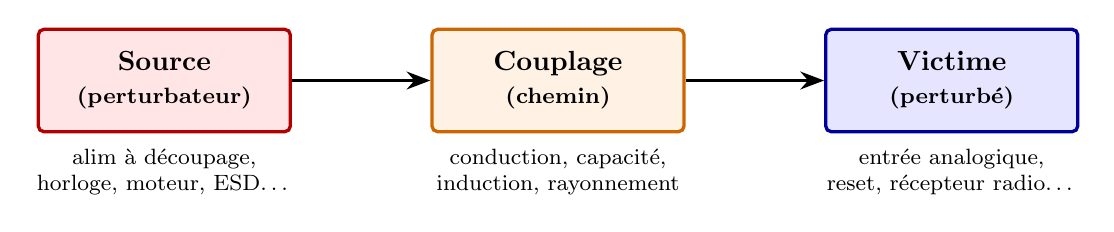
\begin{tikzpicture}[
  bloc/.style={draw, very thick, rounded corners=2pt, minimum width=3.2cm, minimum height=1.3cm, align=center, font=\bfseries},
  fleche/.style={-{Stealth[length=3mm]}, very thick}
]
  \node[bloc, fill=red!10, draw=red!70!black] (src) at (0,0) {Source\\ \footnotesize (perturbateur)};
  \node[bloc, fill=orange!10, draw=orange!80!black] (cpl) at (5,0) {Couplage\\ \footnotesize (chemin)};
  \node[bloc, fill=blue!10, draw=blue!60!black] (vic) at (10,0) {Victime\\ \footnotesize (perturbé)};
  \draw[fleche] (src) -- (cpl);
  \draw[fleche] (cpl) -- (vic);
  \node[below=2pt of src, font=\footnotesize, align=center] {alim à découpage,\\ horloge, moteur, ESD\ldots};
  \node[below=2pt of cpl, font=\footnotesize, align=center] {conduction, capacité,\\ induction, rayonnement};
  \node[below=2pt of vic, font=\footnotesize, align=center] {entrée analogique,\\ reset, récepteur radio\ldots};
\end{tikzpicture}
\caption{Le modèle universel de la CEM : une source, un chemin de couplage, une victime. On peut agir sur chacun des trois blocs.}
\end{figure}

Ce découpage n'est pas qu'une classification : c'est une \textbf{méthode de travail}. Face à une perturbation, on cherche à identifier les trois blocs, puis on choisit où agir :

\begin{itemize}[itemsep=1pt]
  \item \textbf{à la source} : ralentir les fronts inutiles, snubber, routage compact --- c'est presque toujours l'action la plus efficace et la moins chère ;
  \item \textbf{sur le chemin} : éloigner, blinder, filtrer, torsader ;
  \item \textbf{à la victime} : filtrer ses entrées, la rendre moins sensible (hystérésis, bande passante limitée au nécessaire).
\end{itemize}

\subsection{Les quatre chemins de couplage}

L'énergie parasite ne voyage que de quatre façons. Les reconnaître est le premier réflexe du diagnostic.

\begin{enumerate}[itemsep=3pt]
  \item \textbf{Par conduction} : source et victime partagent un conducteur (câble d'alimentation, piste, masse commune). Le parasite voyage \emph{dans les fils}.
  \item \textbf{Par couplage capacitif} : deux conducteurs proches forment un condensateur parasite $C_p$ (chapitre 7). Une variation \emph{de tension} rapide ($\mathrm{d}V/\mathrm{d}t$) chez l'agresseur injecte un courant $i = C_p\,\mathrm{d}V/\mathrm{d}t$ chez la victime.
  \item \textbf{Par couplage inductif} : deux boucles de courant proches forment un transformateur parasite de mutuelle $M$ (chapitre 8). Une variation \emph{de courant} rapide ($\mathrm{d}I/\mathrm{d}t$) chez l'agresseur induit une tension $v = M\,\mathrm{d}I/\mathrm{d}t$ chez la victime.
  \item \textbf{Par rayonnement} : à distance grande devant la taille des circuits et la longueur d'onde réduite (section ingénieur), le champ se détache et se propage comme une onde. Les câbles et les boucles se comportent alors en \textbf{antennes}, à l'émission comme à la réception.
\end{enumerate}

\begin{intuition}
Les couplages capacitif et inductif sont les deux visages d'une même proximité : le premier est piloté par les \textbf{tensions qui varient} (champ électrique entre conducteurs), le second par les \textbf{courants qui varient} (champ magnétique entre boucles). Réflexe de diagnostic : la perturbation suit-elle un n\oe ud à fort $\mathrm{d}V/\mathrm{d}t$ (couplage capacitif) ou une maille à fort $\mathrm{d}I/\mathrm{d}t$ (couplage inductif) ?
\end{intuition}

\subsection{Mode différentiel et mode commun : le concept central}

Sur une liaison à deux fils (aller et retour), le courant peut circuler de deux manières fondamentalement différentes :

\begin{itemize}[itemsep=2pt]
  \item \textbf{Mode différentiel (MD)} : le courant \emph{utile}. Il part par un fil et revient par l'autre : $+I_{\mathrm{MD}}$ à l'aller, $-I_{\mathrm{MD}}$ au retour. C'est le fonctionnement normal de tout circuit.
  \item \textbf{Mode commun (MC)} : un courant \emph{parasite} qui circule dans le \textbf{même sens sur les deux fils} et revient par un chemin extérieur au circuit --- la terre, le châssis, les capacités parasites. Le circuit ne l'a jamais demandé : il naît des imperfections.
\end{itemize}

\begin{figure}[h]
\centering
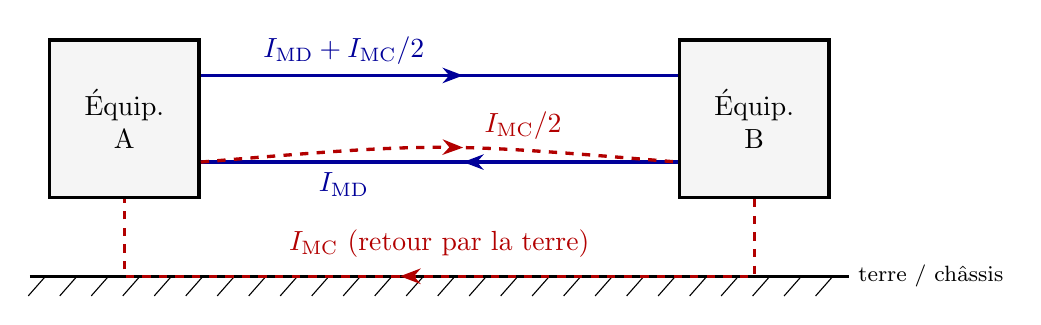
\begin{tikzpicture}[
  fleche/.style={decoration={markings, mark=at position 0.55 with {\arrow{Stealth[length=2.6mm]}}}, postaction={decorate}},
  flecheR/.style={decoration={markings, mark=at position 0.55 with {\arrowreversed{Stealth[length=2.6mm]}}}, postaction={decorate}}
]
  % Equipements
  \node[draw, very thick, minimum width=1.9cm, minimum height=2cm, align=center, fill=gray!8] (A) at (0,0.9) {Équip.\\ A};
  \node[draw, very thick, minimum width=1.9cm, minimum height=2cm, align=center, fill=gray!8] (B) at (8,0.9) {Équip.\\ B};
  % Plan de terre
  \draw[very thick] (-1.2,-1.1) -- (9.2,-1.1);
  \foreach \x in {-1.0,-0.6,...,9.0} \draw (\x,-1.1) -- (\x-0.22,-1.35);
  \node[right] at (9.2,-1.1) {\footnotesize terre / châssis};
  % Fil aller (haut)
  \draw[very thick, fleche, blue!60!black] (A.east |- 0,1.45) -- node[above, pos=0.3, blue!60!black] {$I_{\mathrm{MD}} + I_{\mathrm{MC}}/2$} (B.west |- 0,1.45);
  % Fil retour (bas)
  \draw[very thick, flecheR, blue!60!black] (A.east |- 0,0.35) -- node[below, pos=0.3, blue!60!black] {$I_{\mathrm{MD}}$} (B.west |- 0,0.35);
  \draw[very thick, fleche, red!70!black, dashed] (A.east |- 0,0.35) .. controls (4,0.6) .. node[above, pos=0.72, red!70!black] {$I_{\mathrm{MC}}/2$} (B.west |- 0,0.35);
  % Retour MC par la terre
  \draw[very thick, red!70!black, dashed, fleche]
    (B.south) -- (B.south |- 0,-1.1) -- node[above=3pt, pos=0.5, red!70!black] {$I_{\mathrm{MC}}$ (retour par la terre)} (A.south |- 0,-1.1) -- (A.south);
\end{tikzpicture}
\caption{Mode différentiel (bleu, plein) : aller--retour dans la paire, champs qui se compensent. Mode commun (rouge, pointillé) : même sens sur les deux fils, retour par la terre --- la grande boucle rayonne.}
\end{figure}

Pourquoi cette distinction est-elle \emph{le} concept central de la CEM ?

\begin{itemize}[itemsep=2pt]
  \item En MD, les deux courants opposés créent des champs qui \textbf{se compensent} presque : la paire est discrète.
  \item En MC, les champs des deux fils \textbf{s'ajoutent}, et la boucle de retour (par la terre) est immense : le câble devient une véritable antenne. À courant égal, le MC rayonne des ordres de grandeur de plus que le MD --- on le quantifiera en section ingénieur.
\end{itemize}

\begin{retenir}
La quasi-totalité des échecs en émission rayonnée d'un produit vient de \textbf{courants de mode commun de quelques microampères} sur les câbles. Pas des signaux utiles : de leurs fuites.
\end{retenir}

\subsection{Trois scènes de la vie courante}

\begin{itemize}[itemsep=2pt]
  \item \textbf{Le chargeur qui brouille la radio AM} : l'alimentation à découpage (chapitre 32) injecte ses harmoniques de commutation sur le réseau (conduction) et son câble rayonne le mode commun --- la radio, victime à haute impédance d'entrée, capte tout.
  \item \textbf{La poignée de porte qui redémarre un appareil} : décharge électrostatique (ESD), un front de plusieurs kilovolts en une nanoseconde. Couplage par conduction (dans le châssis) et par rayonnement du front.
  \item \textbf{Le relais qui fait planter le microcontrôleur voisin} : l'ouverture d'une charge inductive (chapitre 8) crée une surtension et un arc, riches en hautes fréquences, couplés par induction et capacité aux pistes voisines.
\end{itemize}

% ============================================================================
\section{Approfondissement}

\begin{approfondissement}
Les modèles quantitatifs des couplages, la naissance du mode commun, le paysage normatif (émission, immunité, moyens d'essai) et le filtre secteur. Prérequis : chapitres 10 (impédances complexes), 13 (spectre, Bode), 32 (découpage).
\end{approfondissement}

\subsection{Couplage capacitif : modèle et remèdes}

Deux conducteurs voisins (pistes parallèles, fils dans un toron) forment une capacité parasite $C_p$ --- typiquement de l'ordre du picofarad pour quelques centimètres de pistes adjacentes. Si l'agresseur porte une tension $v_a(t)$ et la victime présente une impédance $Z_v$ vers sa masse, le diviseur $C_p$--$Z_v$ donne :

\begin{formule}
\[
\underline{V}_v = \frac{Z_v}{Z_v + \dfrac{1}{j\omega C_p}}\ \underline{V}_a
\;\;\xrightarrow[|Z_v| \ll \frac{1}{\omega C_p}]{\text{couplage faible}}\;\;
\underline{V}_v \approx j\omega C_p Z_v\, \underline{V}_a
\]
\[
\text{soit, en temporel : } v_v \approx R_v\, C_p\, \frac{\mathrm{d}v_a}{\mathrm{d}t}
\quad\text{(si } Z_v = R_v \text{ et front lent devant } R_v C_p\text{).}
\]
\end{formule}

Le message physique : la tension induite croît avec la \textbf{fréquence} (ou la raideur du front), avec la \textbf{proximité} (via $C_p$) et avec l'\textbf{impédance de la victime}. Un n\oe ud haute impédance (entrée d'AOP, chapitre 18) est une victime idéale.

\textbf{Remèdes}, par ordre d'efficacité habituelle :
\begin{enumerate}[itemsep=1pt]
  \item réduire $\mathrm{d}v_a/\mathrm{d}t$ à la source si le front est plus raide que nécessaire (résistance série sur une horloge, snubber) ;
  \item \textbf{écran électrostatique} : un conducteur relié à la masse interposé entre les deux --- le courant de $C_p$ est dérivé vers la masse au lieu d'atteindre la victime ;
  \item éloigner ($C_p$ chute vite avec la distance), baisser $Z_v$ quand c'est possible.
\end{enumerate}

\begin{attention}
Un écran \textbf{non relié} (ou relié par un long fil inductif) ne protège presque pas : il se contente de relayer le couplage. L'efficacité d'un écran électrostatique se joue dans la qualité de sa connexion à la masse --- courte et directe.
\end{attention}

\subsection{Couplage inductif : la surface de boucle est l'ennemie}

Une boucle agresseur parcourue par $i_a(t)$ et une boucle victime partagent une mutuelle $M$ (chapitre 8). La tension induite en série dans la boucle victime vaut :

\begin{formule}
\[
v_v(t) = M\,\frac{\mathrm{d}i_a}{\mathrm{d}t},
\qquad M \propto \frac{\text{(surfaces des boucles)} \times \text{(proximité)}}{\text{distance}}
\]
\end{formule}

$M$ n'a pas d'expression simple universelle, mais sa dépendance est claire : elle croît avec les \textbf{surfaces des deux boucles} et leur proximité, et décroît vite avec la distance et le désalignement. D'où les remèdes :

\begin{enumerate}[itemsep=1pt]
  \item \textbf{réduire les surfaces de boucle} --- côté agresseur comme côté victime : conducteur de retour plaqué contre l'aller, paires \textbf{torsadées} (chaque demi-torsade inverse le signe du flux capté : la somme s'annule presque) ;
  \item éloigner, croiser à 90° (flux nul à l'orthogonale) ;
  \item un \textbf{plan de masse} sous les pistes : le courant de retour circule juste sous l'aller (chapitre 36), la surface de boucle devient minuscule.
\end{enumerate}

\begin{intuition}
En CEM, on ne raisonne pas en « fils » mais en \textbf{boucles} : tout courant décrit une boucle fermée, et c'est la \emph{surface} de cette boucle qui couple --- vers l'extérieur (émission) comme depuis l'extérieur (immunité). « Où revient ce courant ? » est \emph{la} question du chapitre 36.
\end{intuition}

\subsection{Couplage par impédance commune : la masse n'est pas équipotentielle}

Quand deux circuits partagent un même conducteur de retour, celui-ci a une impédance $Z_g = R_g + j\omega L_g$ --- et l'inductance domine très vite : un fil ou une piste fine présente grossièrement $\SI{1}{nH}$ par millimètre (ordre de grandeur, géométrie-dépendant). Le courant du circuit 1 crée alors dans $Z_g$ une chute de tension que le circuit 2 voit \textbf{en série avec sa référence} :

\[
v_{\text{parasite}} = Z_g\,(i_1 + i_2)
\quad\Rightarrow\quad
\text{la référence du circuit 2 suit le courant du circuit 1.}
\]

Exemple numérique : $\SI{10}{cm}$ de retour partagé ($L_g \approx \SI{100}{nH}$), un étage numérique qui appelle $\Delta I = \SI{20}{mA}$ en $\SI{2}{ns}$ :
\[
v = L_g \frac{\mathrm{d}i}{\mathrm{d}t} \approx \SI{100e-9}{} \times \frac{\SI{20e-3}{}}{\SI{2e-9}{}} = \SI{1}{V}.
\]
Un volt de rebond de masse --- de quoi corrompre n'importe quel seuil logique ou entrée analogique. C'est le même mécanisme que le \emph{ground bounce} du chapitre 29, étendu à la carte entière.

\textbf{Remèdes} : ne pas partager les retours sensibles et les retours violents (séparation des chemins de courant), raccourcir, élargir, et en haute fréquence utiliser un \textbf{plan} de masse (chapitre 36) dont l'impédance est des ordres de grandeur plus faible qu'une piste.

\subsection{D'où vient le mode commun ?}

Personne ne conçoit un courant de mode commun ; il naît des \textbf{dissymétries} :

\begin{itemize}[itemsep=2pt]
  \item \textbf{Dissymétrie des impédances parasites} : les deux fils d'une paire n'ont pas les mêmes capacités vers le châssis ou la terre ; un signal purement différentiel se convertit partiellement en MC (et réciproquement --- la conversion marche dans les deux sens).
  \item \textbf{Tension de mode commun des alimentations à découpage} : le n\oe ud de commutation (chapitre 32) impose des centaines de volts de $\mathrm{d}V/\mathrm{d}t$ en quelques dizaines de nanosecondes ; à travers la capacité parasite primaire--secondaire du transformateur (dizaines de pF), un courant $i = C_{ps}\,\mathrm{d}V/\mathrm{d}t$ est injecté vers la sortie et revient par la terre : c'est un générateur de MC quasi idéal.
  \item \textbf{Chute de tension sur la masse} (paragraphe précédent) : le potentiel de la « masse » d'une carte oscille par rapport au châssis, et chaque câble qui part de cette carte est excité comme une \textbf{antenne monopole} contre la terre.
\end{itemize}

Cette dernière image est la bonne : \textbf{le câble est le brin rayonnant, la carte est l'excitateur}. On comprend alors pourquoi le remède universel aux échecs en rayonné consiste à traiter les câbles (ferrites de mode commun, blindage, filtrage à la traversée du châssis) et la référence de masse --- pas le signal utile.

\subsection{Le paysage normatif : que mesure-t-on, et comment ?}

Les exigences se répartissent en deux familles, chacune scindée en conduit / rayonné selon le chemin :

\begin{center}
\renewcommand{\arraystretch}{1.35}
\begin{tabular}{p{3.3cm}p{4.6cm}p{5.3cm}}
\toprule
 & \textbf{Émission} & \textbf{Immunité} \\
\midrule
\textbf{Conduit} (via les câbles) & Perturbations réinjectées sur le réseau, $\SI{150}{kHz}$--$\SI{30}{MHz}$, mesurées sur un RSIL & Transitoires rapides en salves (EFT), ondes de choc (foudre), RF conduite, creux de tension \\
\textbf{Rayonné} (via l'air) & Champ électrique émis, $\SI{30}{MHz}$--$\SI{1}{GHz}$ (au-delà si horloges internes rapides), en chambre semi-anéchoïque & Champ RF imposé (émetteurs, radars), décharges électrostatiques (ESD) \\
\bottomrule
\end{tabular}
\end{center}

Quelques repères pour se situer dans la jungle des références :
\begin{itemize}[itemsep=1pt]
  \item \textbf{Émission} : famille CISPR, déclinée en normes européennes EN~550xx (par exemple CISPR~32 / EN~55032 pour les équipements multimédia). Deux classes : \textbf{A} (environnement industriel/commercial, limites plus permissives) et \textbf{B} (résidentiel, plus sévère).
  \item \textbf{Immunité} : série CEI~61000-4-x, chaque essai ayant sa norme : 4-2 (ESD), 4-3 (champ RF), 4-4 (transitoires rapides EFT), 4-5 (ondes de choc), 4-6 (RF conduite)\ldots
  \item Le produit est couvert soit par une \textbf{norme produit} dédiée, soit par les \textbf{normes génériques} (EN~61000-6-1/-2 immunité, -3/-4 émission, selon environnement résidentiel ou industriel).
\end{itemize}

\begin{attention}
Les valeurs chiffrées données dans ce chapitre (gabarits, niveaux d'essai) sont des \textbf{ordres de grandeur typiques} destinés à la conception. Pour une certification, seule fait foi la version en vigueur de la norme applicable au produit --- les limites dépendent de la classe, de la distance de mesure et de l'édition.
\end{attention}

\textbf{Émission conduite --- le RSIL.} On mesure entre $\SI{150}{kHz}$ et $\SI{30}{MHz}$ à travers un \textbf{RSIL} (réseau stabilisateur d'impédance de ligne, LISN en anglais) : un filtre normalisé qui isole l'équipement des parasites du réseau réel et lui présente une impédance reproductible ($\SI{50}{\ohm}$ en HF), sur laquelle on prélève la tension parasite. Ordre de grandeur des limites classe B (quasi-crête) : environ 66~dB\textmu V à $\SI{150}{kHz}$, décroissant vers 56~dB\textmu V à $\SI{500}{kHz}$, puis 56 à 60~dB\textmu V jusqu'à $\SI{30}{MHz}$ --- soit quelques centaines de microvolts à peine sur $\SI{50}{\ohm}$.

\textbf{Émission rayonnée --- la chambre.} De $\SI{30}{MHz}$ à $\SI{1}{GHz}$ (et au-delà pour les produits à horloges rapides), on mesure le champ électrique à distance normalisée (3 ou $\SI{10}{m}$) en chambre semi-anéchoïque, antenne balayée en hauteur et en polarisation.

\begin{figure}[h]
\centering
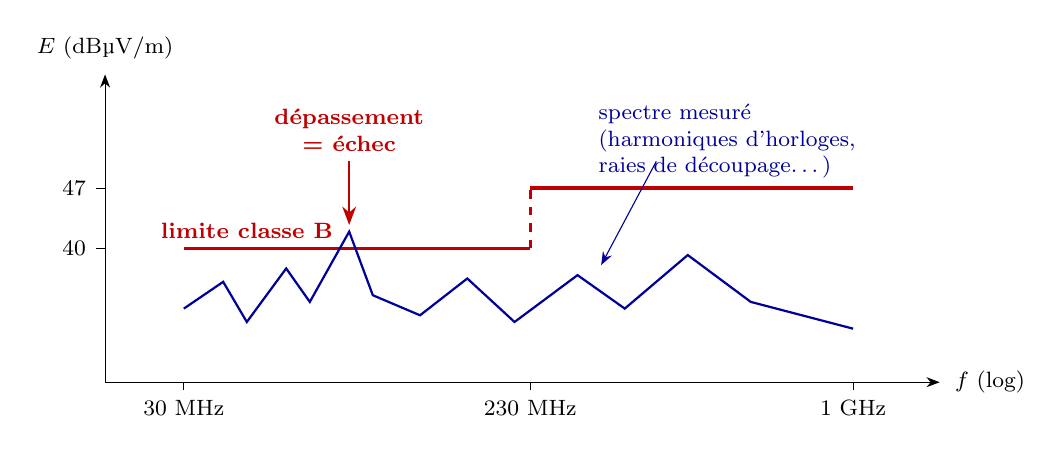
\begin{tikzpicture}[xscale=1.0, yscale=0.85]
  % Axes
  \draw[-{Stealth}] (0,0) -- (10.6,0) node[right=2pt] {\footnotesize $f$ (log)};
  \draw[-{Stealth}] (0,0) -- (0,4.6) node[above=2pt] {\footnotesize $E$ (dB\textmu V/m)};
  % Frequency ticks (log positions): 30M at 1, 230M at ~5.4, 1000M at 9.5
  \foreach \x/\lab in {1/30~MHz, 5.4/230~MHz, 9.5/1~GHz}
    {\draw (\x,0) -- (\x,-0.12) node[below] {\footnotesize \lab};}
  % dB ticks : 40 dB at y=2, 47 dB at y=2.9
  \foreach \y/\lab in {2/40, 2.9/47}
    {\draw (0,\y) -- (-0.12,\y) node[left] {\footnotesize \lab};}
  % Class B template
  \draw[very thick, red!75!black] (1,2) -- (5.4,2);
  \draw[very thick, red!75!black, dashed] (5.4,2) -- (5.4,2.9);
  \draw[very thick, red!75!black] (5.4,2.9) -- (9.5,2.9);
  \node[red!75!black, above, font=\footnotesize\bfseries] at (1.8,2) {limite classe B};
  % A typical spectrum below
  \draw[thick, blue!60!black]
    (1,1.1) -- (1.5,1.5) -- (1.8,0.9) -- (2.3,1.7) -- (2.6,1.2) -- (3.1,2.25) -- (3.4,1.3)
    -- (4.0,1.0) -- (4.6,1.55) -- (5.2,0.9) -- (6.0,1.6) -- (6.6,1.1) -- (7.4,1.9) -- (8.2,1.2) -- (9.5,0.8);
  \node[blue!60!black, font=\footnotesize, align=left] at (7.9,3.6) {spectre mesuré\\ (harmoniques d'horloges,\\ raies de découpage\ldots)};
  \draw[blue!60!black, -{Stealth}] (7.0,3.3) -- (6.3,1.75);
  % Violation marker
  \draw[red!75!black, -{Stealth}, thick] (3.1,3.3) node[above, font=\footnotesize\bfseries, align=center] {dépassement\\ = échec} -- (3.1,2.35);
\end{tikzpicture}
\caption{Principe d'un gabarit d'émission rayonnée (allure type classe B, détecteur quasi-crête, à \SI{3}{m}). Le spectre mesuré doit rester sous la limite sur toute la bande ; une seule raie au-dessus suffit à l'échec.}
\end{figure}

\textbf{Quasi-crête et valeur moyenne.} Le récepteur de mesure normalisé n'utilise pas un simple détecteur crête : le détecteur \textbf{quasi-crête} (QP) pondère les événements selon leur taux de répétition --- héritage de l'époque où le critère était la gêne \emph{audible} sur un récepteur radio : un claquement rare gêne moins qu'un bourdonnement continu, à crête égale. Une perturbation impulsionnelle rare lit donc plus bas en QP qu'en crête ; une raie continue lit pareil. Les limites sont généralement données en QP et en valeur moyenne (AV).

\textbf{Immunité --- niveaux d'essai typiques} (environnement résidentiel, ordres de grandeur) :

\begin{center}
\renewcommand{\arraystretch}{1.3}
\begin{tabular}{p{3.4cm}p{2.6cm}p{6.9cm}}
\toprule
\textbf{Essai} & \textbf{Norme} & \textbf{Sévérité typique (résidentiel)} \\
\midrule
Décharge électrostatique & CEI 61000-4-2 & $\pm\SI{4}{kV}$ contact, $\pm\SI{8}{kV}$ air \\
Champ RF rayonné & CEI 61000-4-3 & $\SI{3}{V/m}$, $\SI{80}{MHz}$--$\SI{1}{GHz}$, modulé AM $80\,\%$ \\
Transitoires rapides (EFT) & CEI 61000-4-4 & $\pm\SI{1}{kV}$ sur l'alimentation, salves $5/\SI{50}{ns}$ \\
Ondes de choc (foudre) & CEI 61000-4-5 & $\pm\SI{1}{kV}$ différentiel, $\pm\SI{2}{kV}$ vers la terre, $1{,}2/\SI{50}{\micro s}$ \\
RF conduite & CEI 61000-4-6 & $\SI{3}{V}$, $\SI{150}{kHz}$--$\SI{80}{MHz}$ \\
\bottomrule
\end{tabular}
\end{center}

Le critère de réussite est gradué : fonctionnement normal pendant l'essai (critère A), dégradation temporaire auto-récupérée (B), ou perte de fonction nécessitant une intervention (C) --- le niveau exigé dépend de la fonction (un airbag n'a pas droit au critère C).

\begin{pratique}
\textbf{Le détail qui piège : la modulation AM de l'essai RF.} Le champ de l'essai 61000-4-3 est modulé en amplitude à $\SI{1}{kHz}$. Toute jonction semi-conductrice non linéaire (entrée d'AOP, jonction base-émetteur --- chapitres 16, 18) peut \textbf{démoduler} cette enveloppe : la perturbation à $\SI{900}{MHz}$ ressort\ldots{} en signal parfaitement audible à $\SI{1}{kHz}$ dans la chaîne audio ou la mesure. C'est le mécanisme du grésillement des anciens amplis près d'un téléphone GSM. Remède : filtrer la RF \emph{avant} la jonction (petit RC ou ferrite directement sur l'entrée).
\end{pratique}

\subsection{Le filtre secteur : l'anatomie d'un classique}

À l'interface entre le réseau et une alimentation à découpage, un filtre traite \emph{séparément} les deux modes :

\begin{figure}[h]
\centering
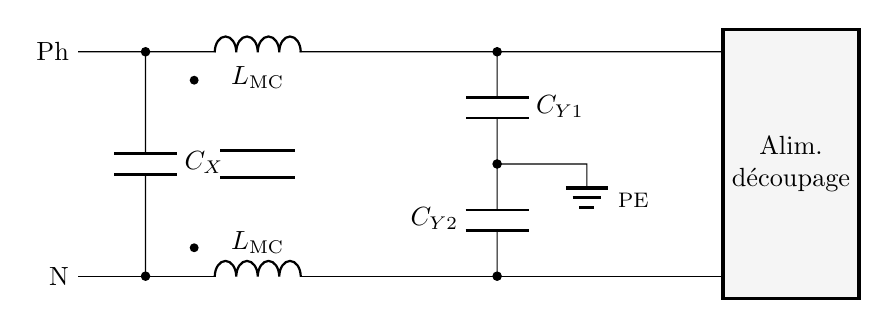
\begin{tikzpicture}[scale=0.95, transform shape]
  % Rails phase et neutre
  \draw (0,3) node[left] {Ph} to[short] (1.4,3)
        to[L, l_=$L_{\mathrm{MC}}$] (3.4,3)
        to[short] (8.6,3);
  \draw (0,0) node[left] {N} to[short] (1.4,0)
        to[L, l^=$L_{\mathrm{MC}}$] (3.4,0)
        to[short] (8.6,0);
  % Noyau commun (deux barres) + points de polarité (sens de bobinage)
  \draw[very thick] (1.9,1.32) -- (2.9,1.32);
  \draw[very thick] (1.9,1.68) -- (2.9,1.68);
  \fill (1.55,2.62) circle (1.7pt);
  \fill (1.55,0.38) circle (1.7pt);
  % Cx entre phase et neutre
  \draw (0.9,3) node[circ]{} to[C, l=$C_X$] (0.9,0) node[circ]{};
  % Condensateurs Y vers PE
  \draw (5.6,3) node[circ]{} to[C, l=$C_{Y1}$] (5.6,1.5);
  \draw (5.6,0) node[circ]{} to[C, l=$C_{Y2}$] (5.6,1.5);
  \draw (5.6,1.5) node[circ]{} to[short] (6.8,1.5) -- (6.8,1.18);
  \draw[very thick] (6.52,1.18) -- (7.08,1.18);
  \draw[very thick] (6.61,1.05) -- (6.99,1.05);
  \draw[very thick] (6.70,0.92) -- (6.90,0.92);
  \node at (7.42,1.02) {\footnotesize PE};
  % Charge
  \node[draw, very thick, minimum width=1.5cm, minimum height=3.6cm, anchor=west, align=center, fill=gray!8] at (8.6,1.5) {Alim.\\ découpage};
\end{tikzpicture}
\caption{Filtre secteur type. $C_X$ (entre phase et neutre) court-circuite le mode différentiel ; la self de mode commun $L_{\mathrm{MC}}$ (deux enroulements sur un même noyau, points de polarité) bloque le MC ; les condensateurs $C_Y$ renvoient le courant de MC vers la terre de protection PE.}
\end{figure}

\begin{itemize}[itemsep=2pt]
  \item \textbf{$C_X$} (classe de sécurité X, entre phase et neutre) : basse impédance pour le \textbf{mode différentiel} --- il court-circuite les harmoniques de découpage avant qu'elles ne sortent. Valeurs typiques : $\SI{100}{nF}$ à quelques \si{\micro F}.
  \item \textbf{Self de mode commun $L_{\mathrm{MC}}$} : deux enroulements sur le même noyau, bobinés de sorte que les flux du courant \emph{différentiel} s'annulent (le noyau ne le voit pas : pas de saturation par le courant utile) tandis que les flux du courant de \emph{mode commun} s'ajoutent --- le MC voit une forte inductance (du \si{mH} typiquement). L'imperfection du couplage laisse une \textbf{inductance de fuite} de quelques \si{\micro H}\ldots{} qui sert opportunément de filtre MD.
  \item \textbf{$C_Y$} (classe Y, vers la terre) : offrent au courant de MC un chemin de retour court vers PE, avant le câble. Leur valeur est \textbf{plafonnée par la sécurité} : ils injectent en permanence un courant de fuite $I = \omega C_Y U_{\text{secteur}}$ dans le conducteur de protection, limité par les normes produit (typiquement quelques centaines de \si{\micro A} à quelques \si{mA} ; bien plus sévère en médical). D'où des $C_Y$ de l'ordre du nanofarad seulement --- et la classe Y garantit qu'une défaillance ne met pas la phase sur la carcasse.
\end{itemize}

\begin{attention}
L'atténuation d'un filtre du commerce est spécifiée entre source et charge de $\SI{50}{\ohm}$ --- des impédances que ni le réseau ni votre alimentation ne présentent. Un filtre peut même \textbf{amplifier} par résonance autour de sa fréquence propre si les impédances réelles s'y prêtent (chapitre 12) et si rien ne l'amortit. Les décibels du catalogue sont un point de comparaison, pas une garantie d'installation.
\end{attention}

% ============================================================================
\section{Niveau Ingénieur}

\begin{ingenieur}
La physique du rayonnement (pourquoi les microampères de MC dominent), champ proche et champ lointain, la théorie du blindage et sa vraie limite (les ouvertures), les stratégies de masse, l'ESD et le débogage. Prérequis : chapitres 8--9, 13, 29, 32.
\end{ingenieur}

\subsection{Physique du rayonnement : la boucle et le fil}

\textbf{Hypothèses.} Structures petites devant la longueur d'onde ($\ell \ll \lambda$), courant supposé uniforme, observation en champ lointain, orientation la plus défavorable. Ce sont les modèles élémentaires du \emph{petit dipôle magnétique} (boucle) et du \emph{petit dipôle électrique} (fil), suffisants pour prédire des ordres de grandeur remarquablement fiables.

\textbf{Le courant différentiel rayonne par sa boucle.} Une boucle de surface $A$ parcourue par $I_{\mathrm{MD}}$ à la fréquence $f$ crée à la distance $r$, en espace libre, un champ électrique maximal :

\begin{formule}
\[
E_{\mathrm{MD}} \approx \num{1.32e-14}\;\frac{f^2\, A\, I_{\mathrm{MD}}}{r}
\qquad
\left[\si{V/m}\right],\ f\ \text{en Hz},\ A\ \text{en } \si{m^2},\ I\ \text{en A},\ r\ \text{en m}
\]
\end{formule}

La dépendance en $f^2$ vient de deux dérivations successives : le rayonnement est piloté par la \emph{variation} du moment magnétique, lui-même proportionnel à la fréquence dans le passage au champ lointain. Conséquence pratique : ce sont les \textbf{harmoniques élevées} des fronts (chapitre 29) qui rayonnent, pas le fondamental.

\textbf{Le courant de mode commun rayonne par son câble.} Un conducteur de longueur $L$ (le câble) parcouru par $I_{\mathrm{MC}}$ se comporte en petit dipôle électrique :

\begin{formule}
\[
E_{\mathrm{MC}} \approx \num{6.3e-7}\;\frac{f\, L\, I_{\mathrm{MC}}}{r}
\qquad
\left[\si{V/m}\right],\ \text{mêmes unités.}
\]
\end{formule}

(Les essais normalisés se déroulant au-dessus d'un plan de sol réfléchissant, le pire cas mesuré peut atteindre le double de ces valeurs d'espace libre ; l'ordre de grandeur reste le même. Ces deux expressions cessent d'être valables quand $L$ ou $\sqrt{A}$ approchent $\lambda/4$ : la structure devient une antenne résonante et rayonne encore mieux.)

\begin{pratique}
\textbf{Cas réel complet --- combien de courant pour échouer ?} Limite d'allure classe B à $\SI{3}{m}$ : $40$~dB\textmu V/m $= \SI{100}{\micro V/m}$ à $f = \SI{50}{MHz}$.

\textbf{Mode commun}, câble de $L = \SI{1}{m}$ :
\[
I_{\mathrm{MC}} = \frac{E\,r}{\num{6.3e-7}\,f\,L}
= \frac{\num{1e-4} \times 3}{\num{6.3e-7} \times \num{5e7} \times 1}
\approx \SI{10}{\micro A}
\]
(à diviser par $\sim 2$ au-dessus du plan de sol de l'essai : $\approx \SI{5}{\micro A}$).

\textbf{Mode différentiel}, boucle de $A = \SI{10}{cm^2} = \SI{1e-3}{m^2}$ :
\[
I_{\mathrm{MD}} = \frac{E\,r}{\num{1.32e-14}\,f^2\,A}
= \frac{\num{3e-4}}{\num{1.32e-14} \times \num{2.5e15} \times \num{1e-3}}
\approx \SI{9}{mA}.
\]

\textbf{Trois ordres de grandeur d'écart.} Cinq à dix microampères de mode commun sur un câble suffisent à faire échouer un essai que dix milliampères de courant différentiel bien routé passeraient. C'est la justification quantitative du réflexe « en rayonné, traiter d'abord les câbles et le mode commun ».
\end{pratique}

\subsection{Champ proche, champ lointain : quelle est la nature du champ ?}

Autour d'une source, la structure du champ change avec la distance. La frontière se situe vers :

\begin{formule}
\[
r_{\text{transition}} \approx \frac{\lambda}{2\pi}
\qquad\text{(soit } \approx \SI{48}{cm} \text{ à } \SI{100}{MHz},\ \approx \SI{4.8}{m} \text{ à } \SI{10}{MHz}).
\]
\end{formule}

\begin{itemize}[itemsep=2pt]
  \item \textbf{Champ lointain} ($r \gg \lambda/2\pi$) : onde plane locale, $E$ et $H$ liés par l'impédance d'onde du vide $Z_w = E/H = \eta_0 \approx \SI{377}{\ohm}$, décroissance en $1/r$.
  \item \textbf{Champ proche} ($r \ll \lambda/2\pi$) : le champ garde la personnalité de sa source. Une source à \textbf{haute impédance} (dipôle, n\oe ud à fort $\mathrm{d}V/\mathrm{d}t$) impose un champ dominé par $E$ : $Z_w \gg \SI{377}{\ohm}$. Une source à \textbf{basse impédance} (boucle, maille à fort $\mathrm{d}I/\mathrm{d}t$) impose un champ dominé par $H$ : $Z_w \ll \SI{377}{\ohm}$. Les composantes réactives décroissent vite ($1/r^2$, $1/r^3$) : c'est le régime des couplages capacitif et inductif des sections précédentes, qui apparaissent ainsi comme le \emph{cas limite proche} du rayonnement.
\end{itemize}

\begin{figure}[h]
\centering
\begin{tikzpicture}[xscale=1.05, yscale=0.9]
  % axes
  \draw[-{Stealth}] (0,0) -- (9.8,0) node[right=2pt] {\footnotesize $r$ (log)};
  \draw[-{Stealth}] (0,0) -- (0,4.6) node[above=2pt] {\footnotesize $Z_w = E/H$ (log)};
  % 377 ohm line
  \draw[dashed, thick] (0,2.2) -- (9.5,2.2) node[pos=0.1, below, font=\footnotesize] {$\eta_0 = \SI{377}{\ohm}$};
  % transition vertical
  \draw[dashed, thick] (5.4,0) -- (5.4,4.3);
  \node[below, font=\footnotesize] at (5.4,0) {$\lambda/2\pi$};
  % E-source curve (high Z, decreasing to 377)
  \draw[very thick, red!75!black] (0.7,3.75) .. controls (3.4,3.2) and (4.6,2.5) .. (5.4,2.28)
        .. controls (6.2,2.16) and (7.0,2.2) .. (9.3,2.2);
  \node[red!75!black, font=\footnotesize, align=center] at (2.7,4.15) {source « électrique »\\ (fort $\mathrm{d}V/\mathrm{d}t$) : $Z_w$ élevée};
  % H-source curve (low Z, rising to 377)
  \draw[very thick, blue!60!black] (0.7,0.75) .. controls (3.4,1.2) and (4.6,1.9) .. (5.4,2.12)
        .. controls (6.2,2.24) and (7.0,2.2) .. (9.3,2.2);
  \node[blue!60!black, font=\footnotesize, align=center] at (3.4,0.42) {source « magnétique »\\ (fort $\mathrm{d}I/\mathrm{d}t$) : $Z_w$ faible};
  % regions
  \node[font=\footnotesize\itshape] at (2.7,2.55) {champ proche};
  \node[font=\footnotesize\itshape] at (7.6,2.55) {champ lointain};
\end{tikzpicture}
\caption{Impédance d'onde en fonction de la distance à la source (échelles log). En champ proche, la nature du champ ($E$ ou $H$ dominant) dépend de la source ; au-delà de $\lambda/2\pi$, tout converge vers l'onde plane à $\SI{377}{\ohm}$.}
\end{figure}

Cette classification n'est pas académique : elle détermine \textbf{quel remède fonctionne}. Un champ proche magnétique basse fréquence (transformateur $\SI{50}{Hz}$) traverse une feuille de cuivre comme si elle n'existait pas ; un champ électrique haute impédance est arrêté par le moindre écran relié. Voyons pourquoi.

\subsection{Le blindage : théorie\ldots}

\textbf{Hypothèses.} Écran conducteur plan, infini, homogène, d'épaisseur $t$, onde incidente normale --- le modèle de Schelkunoff, transposition directe des lignes de transmission (l'écran est un tronçon de « ligne » désadaptée). L'efficacité de blindage (SE, \emph{shielding effectiveness}) en décibels se décompose :

\begin{formule}
\[
\mathrm{SE} = R + A + B \quad [\si{dB}]
\]
$R$ : pertes par \textbf{réflexion} (désadaptation d'impédance onde/métal) ; $A$ : pertes par \textbf{absorption} dans l'épaisseur ; $B$ : correction de réflexions multiples internes (négligeable dès que $A \gtrsim \SI{10}{dB}$).
\end{formule}

\textbf{Absorption.} L'onde décroît dans le métal en $e^{-t/\delta}$, où $\delta$ est l'épaisseur de peau (chapitre 9) :
\[
\delta = \frac{1}{\sqrt{\pi f \mu \sigma}}
\quad\Rightarrow\quad
A = 8{,}69\,\frac{t}{\delta}\ [\si{dB}]
\qquad
\delta_{\mathrm{Cu}} \approx \frac{\SI{66}{\micro m}}{\sqrt{f\,[\si{MHz}]}}
\ \ (\SI{9.3}{mm}\ \text{à}\ \SI{50}{Hz},\ \SI{66}{\micro m}\ \text{à}\ \SI{1}{MHz}).
\]

\textbf{Réflexion.} $R$ croît avec la désadaptation entre l'impédance d'onde incidente $Z_w$ et l'impédance intrinsèque du métal $Z_m = \sqrt{\pi f \mu / \sigma}$ (quelques centaines de \si{\micro\ohm} pour le cuivre en HF). Pour une onde plane sur du cuivre : $R \approx \SI{108}{dB}$ à $\SI{1}{MHz}$, encore $\approx \SI{88}{dB}$ à $\SI{100}{MHz}$. Trois conséquences structurantes :

\begin{itemize}[itemsep=2pt]
  \item \textbf{Champ E, haute impédance} : désadaptation énorme avec le métal $\Rightarrow$ $R$ colossal. Le plus mince des écrans reliés suffit (c'est l'écran électrostatique de la section précédente).
  \item \textbf{Champ H basse fréquence, basse impédance} : $R$ faible \emph{et} $\delta$ centimétrique $\Rightarrow$ ni la réflexion ni l'absorption ne fonctionnent. On ne « bloque » pas un champ magnétique à $\SI{50}{Hz}$ : on le \textbf{détourne} dans un matériau à haute perméabilité (mu-métal, $\mu_r \sim 10^4$--$10^5$) qui offre au flux un chemin préférentiel, ou on éloigne/réduit la boucle source.
  \item \textbf{Au-dessus du mégahertz}, n'importe quelle tôle conductrice donne un SE théorique supérieur à $\SI{100}{dB}$ --- très au-delà des besoins. \textbf{Le matériau n'est donc jamais le facteur limitant d'un blindage HF réel.}
\end{itemize}

\subsection{\ldots et sa vraie limite : les ouvertures}

Un boîtier réel a des fentes (couvercle, connecteurs, aération), et c'est par elles que tout fuit. Le résultat contre-intuitif essentiel :

\begin{retenir}
La fuite d'une fente dépend de sa \textbf{plus grande dimension}, pas de sa surface. Une fente fine et longue (jointure de capot mal contactée) fuit comme une ouverture béante de même longueur : les courants de peau qui devaient circuler sur l'écran sont interrompus \emph{sur toute la longueur} de la fente, qui se comporte en \textbf{antenne à fente} --- résonante (SE $\to$ 0) quand $L = \lambda/2$.
\end{retenir}

Pour une fente de longueur $L \le \lambda/2$, l'ordre de grandeur classique :
\[
\mathrm{SE}_{\text{fente}} \approx 20\log_{10}\!\left(\frac{\lambda}{2L}\right)\ [\si{dB}]
\]
et pour $n$ ouvertures identiques proches (espacement $\ll \lambda$), le SE diminue d'environ $10\log_{10} n$.

Exemple : jointure de $\SI{15}{cm}$ sans contact intermédiaire, à $\SI{600}{MHz}$ ($\lambda = \SI{50}{cm}$) : $\mathrm{SE} \approx 20\log(50/30) \approx \SI{4}{dB}$. Le boîtier « métallique » est pratiquement transparent --- quel que soit son matériau. D'où les règles de construction :

\begin{itemize}[itemsep=2pt]
  \item \textbf{fractionner} : points de contact (vis, clips, joint conducteur) à intervalle $\ll \lambda_{\min}/2$ de la fréquence la plus haute à contenir --- viser $\lambda/20$ à $\lambda/50$ pour un SE utile ;
  \item \textbf{aération en guide sous coupure} : un trou profond ($t$) et étroit ($d$) est un guide d'onde utilisé sous sa fréquence de coupure ($f_c \approx 176/d\,[\si{mm}]$ en \si{GHz} pour un trou rond) : atténuation $\approx 32\,t/d$~dB, indépendante de la fréquence tant que $f \ll f_c$. C'est le principe des grilles nid-d'abeilles : beaucoup de petits trous profonds plutôt qu'une grande ouverture ;
  \item \textbf{traiter les câbles à la traversée} : un câble qui traverse l'écran sans précaution est la pire des ouvertures --- il ramène l'antenne \emph{à travers} le blindage. Blindage du câble repris à $360°$ sur le châssis (presse-étoupe CEM), ou filtrage traversant (condensateurs \emph{feedthrough}) au passage de paroi.
\end{itemize}

\begin{attention}
\textbf{Le « pigtail » ruine le blindage.} Reprendre la tresse d'un câble blindé par un petit fil queue-de-cochon de quelques centimètres insère $\sim$ dizaines de \si{nH} en série : à $\SI{100}{MHz}$, plusieurs dizaines d'ohms, alors que l'efficacité du blindage repose sur une reprise de quelques milliohms. La qualité d'un câble blindé se caractérise d'ailleurs par son \textbf{impédance de transfert} $Z_t$ (tension induite à l'intérieur par ampère de courant de gaine, par mètre) : une reprise en pigtail multiplie le $Z_t$ effectif par des ordres de grandeur. La règle : reprise périphérique $360°$, directement sur le châssis, à l'entrée du boîtier.
\end{attention}

\begin{pratique}
\textbf{Perspective : le blindage sélectif.} Un écran n'est pas condamné à tout bloquer : en structurant sa surface en motifs conducteurs périodiques (\emph{surfaces sélectives en fréquence}, et plus généralement \textbf{métasurfaces}), on réalise des parois qui réfléchissent certaines bandes et en laissent passer --- voire en \emph{récupèrent} --- d'autres. C'est un axe de recherche actif : radômes filtrants, fenêtres blindées, et écrans qui convertissent l'énergie RF incidente au lieu de la dissiper.
\end{pratique}

\subsection{Stratégies de masse : basse fréquence contre haute fréquence}

D'abord distinguer trois notions que le langage courant confond :

\begin{itemize}[itemsep=1pt]
  \item la \textbf{masse signal} (0~V) : référence de potentiel des circuits ;
  \item le \textbf{châssis} : l'enveloppe conductrice mécanique (et l'écran, quand il y en a un) ;
  \item la \textbf{terre de protection} (PE) : conducteur de sécurité électrique --- son rôle premier est de protéger les personnes, pas les signaux.
\end{itemize}

Leur interconnexion est un choix de conception, et le bon choix dépend de la fréquence, parce que l'impédance des liaisons est inductive ($\sim\SI{1}{nH/mm}$) :

\begin{itemize}[itemsep=3pt]
  \item \textbf{Basse fréquence (audio, instrumentation, $\lesssim$ centaines de kHz)} : masse en \textbf{point unique} (étoile). On maîtrise le chemin de chaque courant de retour, et surtout on évite les \textbf{boucles de masse} : deux équipements reliés à la terre en deux points distants, plus une liaison signal entre eux, forment une boucle géante ; le flux à $\SI{50}{Hz}$ qui la traverse et les courants vagabonds de terre y injectent une tension \emph{en série avec le signal} (couplage par impédance commune à l'échelle de l'installation). C'est le ronflement des chaînes audio.
  \item \textbf{Haute fréquence ($\gtrsim$ MHz)} : le point unique devient une fiction --- l'inductance du moindre fil de retour isole les masses ($\SI{10}{cm} \Rightarrow \sim\SI{100}{nH} \Rightarrow \SI{63}{\ohm}$ à $\SI{100}{MHz}$), et les capacités parasites referment de toute façon les boucles qu'on croyait avoir ouvertes. On passe en \textbf{multipoint} : toutes les masses au châssis/plan, par des liaisons courtes ($\ll \lambda/20$), le plan de masse faisant équipotentielle.
  \item \textbf{Systèmes mixtes} : masse \textbf{hybride} --- liaison directe là où il le faut, condensateurs (transparents en HF, ouverts en BF) ou selfs/ferrites (l'inverse) pour offrir à chaque bande le schéma qui lui convient.
\end{itemize}

Quand une boucle de masse est inévitable (deux bâtiments, deux racks), on la \textbf{rompt pour le signal} sans la rompre pour la sécurité : transformateur d'isolement, optocoupleur, liaison différentielle à forte réjection de mode commun (RS-485, chapitre 28), ou self de mode commun sur la liaison.

\subsection{Immunité : l'ESD, le front le plus raide du système}

La décharge électrostatique est l'agression de référence : un corps humain chargé à plusieurs kilovolts se décharge dans le produit. La forme d'onde normalisée (CEI 61000-4-2, décharge contact) monte en \textbf{moins d'une nanoseconde} --- environ $3{,}75\,\si{A}$ de premier pic par kilovolt de charge, soit $\SI{30}{A}$ à $\SI{8}{kV}$ --- puis s'éteint en quelques dizaines de nanosecondes.

\begin{figure}[h]
\centering
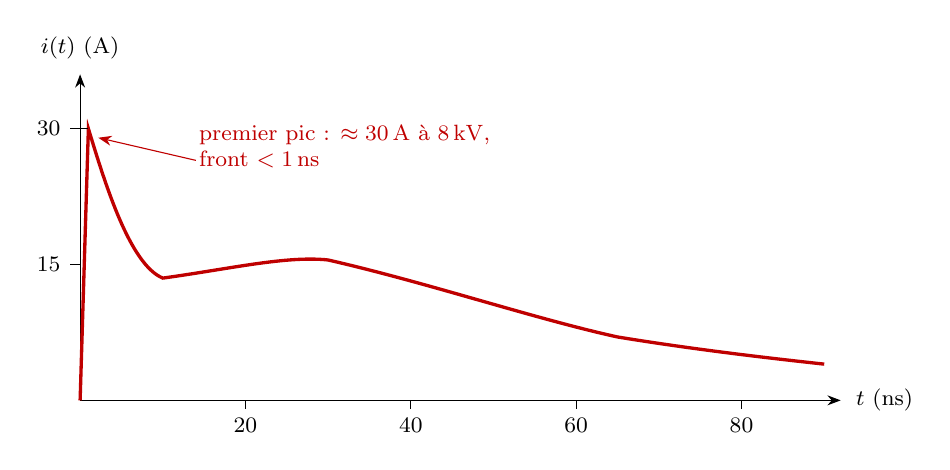
\begin{tikzpicture}[xscale=0.105, yscale=0.115]
  % axes
  \draw[-{Stealth}] (0,0) -- (92,0) node[right=2pt] {\footnotesize $t$ (ns)};
  \draw[-{Stealth}] (0,0) -- (0,36) node[above=2pt] {\footnotesize $i(t)$ (A)};
  \foreach \x in {20,40,60,80} \draw (\x,0) -- (\x,-0.9) node[below] {\footnotesize \x};
  \foreach \y/\lab in {15/15, 30/30} \draw (0,\y) -- (-1.2,\y) node[left] {\footnotesize \lab};
  % waveform: sharp 1ns rise to 30, fast fall to ~14, hump ~16 at 30 ns, decay to ~7 at 60
  \draw[very thick, red!75!black]
    (0,0) -- (1,30)
    .. controls (3,24) and (6,15) .. (10,13.5)
    .. controls (18,14.5) and (25,16) .. (30,15.5)
    .. controls (42,13) and (55,9) .. (65,7)
    .. controls (75,5.5) and (85,4.5) .. (90,4);
  \draw[dashed] (0,30) -- (1,30);
  \node[red!75!black, font=\footnotesize, align=left] at (32,28) {premier pic : $\approx \SI{30}{A}$ à $\SI{8}{kV}$,\\ front $< \SI{1}{ns}$};
  \draw[red!75!black, -{Stealth}] (14,26.5) -- (2.2,29);
\end{tikzpicture}
\caption{Allure du courant de décharge ESD normalisé (contact, $\SI{8}{kV}$). Le front subnanoseconde porte un contenu spectral significatif jusqu'au gigahertz : l'ESD est à la fois un problème de conduction et de rayonnement.}
\end{figure}

Un front de $t_r \approx \SI{1}{ns}$ a un contenu spectral significatif jusqu'à $f \approx 1/(\pi t_r) \approx \SI{300}{MHz}$ et au-delà (chapitre 29) : pendant la décharge, chaque piste est une antenne réceptrice et chaque centimètre d'inductance compte ($\SI{30}{A}$ dans $\SI{10}{nH}$ en $\SI{1}{ns}$ : $\SI{300}{V}$). La stratégie de protection est toujours la même :

\begin{enumerate}[itemsep=2pt]
  \item \textbf{Dériver le courant vers le châssis} par le chemin le plus court, \emph{sans} qu'il traverse l'électronique : c'est un problème de routage avant d'être un problème de composant (anneau de garde périphérique, connecteurs au châssis --- chapitre 36).
  \item \textbf{Écrêter} au plus près du point d'entrée : diode TVS (une diode de puissance conçue pour l'avalanche répétitive, chapitre 15) choisie pour une tension de veille au-dessus du signal et une tension d'écrêtage sous la limite du circuit protégé --- en tenant compte de l'inductance série qui s'ajoute à l'écrêtage ($V = V_{\text{clamp}} + L\,\mathrm{d}i/\mathrm{d}t$ : quelques centimètres de piste ruinent la meilleure TVS).
  \item \textbf{Ralentir et dissiper} ce qui reste : ferrite ou résistance série + condensateur vers la masse, formant un passe-bas pour le front résiduel.
\end{enumerate}

\subsection{Mesurer et déboguer : la CEM au quotidien}

Attendre le laboratoire accrédité pour découvrir un échec est la pire stratégie. La \textbf{pré-conformité} au bureau d'études repose sur trois outils :

\begin{itemize}[itemsep=2pt]
  \item \textbf{Analyseur de spectre + RSIL} : reproduire la mesure d'émission conduite sur table --- valeurs absolues approximatives, mais parfaites pour comparer avant/après une modification.
  \item \textbf{Sondes de champ proche} (petites boucles pour $H$, pointes pour $E$) : promener la sonde sur la carte pour \emph{localiser} les sources et les fuites --- qualitatif mais redoutablement efficace, car en champ proche l'amplitude chute vite avec la distance : ce que la sonde voit fort est dessous.
  \item \textbf{Pince de courant RF} sur les câbles : mesurer directement $I_{\mathrm{MC}}$. C'est le meilleur prédicteur d'un essai rayonné : la règle d'or dérivée du calcul de la section précédente --- \textbf{quelques microampères par câble au maximum} sur les fréquences critiques --- se vérifie à la pince avant de payer la chambre.
\end{itemize}

La démarche de débogage suit le triptyque : identifier la fréquence en défaut (elle signe la source : harmonique d'horloge ? raie de découpage ?), localiser à la sonde, identifier le chemin (couper/débrancher les câbles un à un est le test le plus informatif qui soit), puis traiter --- source, chemin ou victime.

% ============================================================================
\section*{Exercices}
\addcontentsline{toc}{section}{Exercices}

\subsection*{Niveau débutant}

\textbf{Exercice 35.1 ---} Pour chaque situation, identifiez le chemin de couplage dominant : (a) un variateur de vitesse fait apparaître des parasites sur un capteur dont le câble chemine dans la même goulotte, parallèle sur $\SI{2}{m}$ ; (b) une perceuse fait grésiller un poste de radio FM situé dans une autre pièce ; (c) deux circuits d'une même carte partagent $\SI{8}{cm}$ de piste de masse, et le premier fait osciller la référence du second.

\begin{pratique}
\textbf{Solution :}

(a) \textbf{Couplage réactif de proximité} (capacitif et/ou inductif) : longueur parallèle importante, faible distance. Les forts $\mathrm{d}V/\mathrm{d}t$ du variateur privilégient le capacitif ; ses forts $\mathrm{d}I/\mathrm{d}t$ l'inductif --- torsader le câble capteur et l'éloigner traite les deux.

(b) \textbf{Rayonnement} : pas de liaison ni de proximité ; les arcs des balais du moteur émettent un spectre large capté par l'antenne du récepteur.

(c) \textbf{Impédance commune} : le courant du premier circuit crée une chute de tension dans la piste de masse partagée, vue en série par la référence du second.
\end{pratique}

\textbf{Exercice 35.2 ---} Calculez la distance de transition champ proche / champ lointain $\lambda/2\pi$ à $\SI{10}{MHz}$ et à $\SI{1}{GHz}$. Une sonde placée à $\SI{1}{m}$ d'une carte est-elle en champ proche ou lointain à ces deux fréquences ?

\begin{pratique}
\textbf{Solution :}

À $\SI{10}{MHz}$ : $\lambda = c/f = \SI{30}{m}$, donc $\lambda/2\pi \approx \SI{4.8}{m}$. À $\SI{1}{GHz}$ : $\lambda = \SI{30}{cm}$, donc $\lambda/2\pi \approx \SI{4.8}{cm}$.

À $\SI{1}{m}$ : \textbf{champ proche} à $\SI{10}{MHz}$ ($1 < 4{,}8\,\si{m}$) --- le champ dépend de la nature de la source ; \textbf{champ lointain} à $\SI{1}{GHz}$ ($1 \gg 0{,}048\,\si{m}$) --- onde plane locale, $Z_w \approx \SI{377}{\ohm}$.
\end{pratique}

\subsection*{Niveau intermédiaire}

\textbf{Exercice 35.3 ---} Une piste d'horloge ($\SI{3.3}{V}$, fronts de $\SI{2}{ns}$) court parallèlement à une piste analogique sur quelques centimètres : $C_p = \SI{2}{pF}$. La piste victime présente $R_v = \SI{100}{\ohm}$ vers la masse. (a) Vérifiez que l'approximation « couplage faible » est licite, puis estimez la tension parasite crête. (b) Un écran (piste de garde reliée à la masse) réduit $C_p$ à $\SI{0.2}{pF}$ : nouvelle amplitude ? (c) Concluez vis-à-vis d'une marge de bruit logique de $\SI{0.4}{V}$.

\begin{pratique}
\textbf{Solution :}

(a) Constante de couplage : $R_v C_p = 100 \times \SI{2e-12}{} = \SI{0.2}{ns} \ll t_r = \SI{2}{ns}$ : l'approximation dérivateur est licite.
\[
v_v \approx R_v\,C_p\,\frac{\mathrm{d}v_a}{\mathrm{d}t} = 100 \times \SI{2e-12}{} \times \frac{3{,}3}{\SI{2e-9}{}} \approx \SI{0.33}{V}.
\]

(b) $C_p$ divisé par 10 $\Rightarrow$ $v_v \approx \SI{33}{mV}$ (la relation est linéaire en $C_p$).

(c) Sans garde, $\SI{0.33}{V}$ consomme l'essentiel d'une marge de $\SI{0.4}{V}$ : tout bruit additionnel (rebond de masse\ldots) fait franchir le seuil. Avec la garde, un ordre de grandeur de sécurité. Et l'action \emph{à la source} reste disponible : si l'horloge tolère des fronts de $\SI{10}{ns}$, une résistance série divise encore le couplage par 5.
\end{pratique}

\textbf{Exercice 35.4 ---} Un filtre secteur utilise deux condensateurs $C_Y = \SI{2.2}{nF}$ entre chaque conducteur et la terre. Réseau : $\SI{230}{V}$ / $\SI{50}{Hz}$. (a) Calculez le courant de fuite permanent dans le conducteur de protection (cas défavorable : les deux contributions s'ajoutent). (b) La norme produit limite la fuite à $\SI{0.5}{mA}$ : le choix est-il acceptable ? (c) Même question pour un dispositif médical limité à $\SI{100}{\micro A}$ --- que proposez-vous ?

\begin{pratique}
\textbf{Solution :}

(a) $I = \omega\,(2 C_Y)\, U = 2\pi \times 50 \times \SI{4.4e-9}{} \times 230 \approx \SI{0.32}{mA}$.

(b) $0{,}32 < \SI{0.5}{mA}$ : acceptable, mais marge faible ($36\,\%$) --- les tolérances des condensateurs ($\pm 20\,\%$) et la tension réseau haute ($253\,\si{V}$) la consomment presque : à vérifier au pire cas ($\approx \SI{0.42}{mA}$ : passe encore, de justesse).

(c) $\SI{0.32}{mA} \gg \SI{100}{\micro A}$ : refusé. Réduire à $C_Y = \SI{470}{pF}$ ($I \approx \SI{68}{\micro A}$ au nominal) et \textbf{compenser le filtrage MC perdu autrement} : self de mode commun plus grosse, voire second étage --- l'arbitrage sécurité/CEM est structurel en médical.
\end{pratique}

\subsection*{Niveau ingénieur}

\textbf{Exercice 35.5 ---} Un produit doit tenir une limite d'allure classe B de $40$~dB\textmu V/m à $\SI{3}{m}$, à $f = \SI{100}{MHz}$. (a) Quel courant de mode commun maximal admet un câble de $L = \SI{1}{m}$ (formule espace libre) ? (b) Quel courant différentiel admettrait une boucle de $\SI{5}{cm^2}$ ? (c) Le produit échoue de $\SI{10}{dB}$ à cette fréquence, et la pince RF mesure $\SI{8}{\micro A}$ sur le câble d'alimentation : le câble suffit-il à expliquer l'échec, et de quel facteur faut-il réduire $I_{\mathrm{MC}}$ ?

\begin{pratique}
\textbf{Solution :}

(a) $E = \SI{100}{\micro V/m}$, d'où
$I_{\mathrm{MC}} = \dfrac{E\,r}{\num{6.3e-7}\,f\,L} = \dfrac{\num{3e-4}}{\num{6.3e-7} \times \num{1e8} \times 1} \approx \SI{4.8}{\micro A}.$

(b) $I_{\mathrm{MD}} = \dfrac{E\,r}{\num{1.32e-14}\,f^2\,A} = \dfrac{\num{3e-4}}{\num{1.32e-14} \times \num{1e16} \times \num{5e-4}} \approx \SI{4.5}{mA}$ --- trois ordres de grandeur au-dessus.

(c) $\SI{8}{\micro A}$ mesurés contre $\approx \SI{4.8}{\micro A}$ admissibles : le champ attendu du seul câble dépasse la limite d'environ $20\log(8/4{,}8) \approx \SI{4.4}{dB}$ --- le câble est un contributeur majeur mais n'explique pas les $\SI{10}{dB}$ à lui seul (autre câble ? fente ?). Pour revenir $\SI{10}{dB}$ sous la mesure actuelle, il faut diviser le courant total rayonnant par $10^{10/20} \approx 3{,}2$ --- soit viser $\lesssim \SI{2.5}{\micro A}$ par câble : typiquement une ferrite de mode commun ($Z \gtrsim$ quelques centaines d'ohms à $\SI{100}{MHz}$) au plus près de la sortie, et vérification à la pince des autres câbles.
\end{pratique}

\textbf{Exercice 35.6 ---} Le capot d'un boîtier n'est vissé qu'à ses quatre coins : la jointure laisse une fente continue de $L = \SI{15}{cm}$ par côté. Le produit contient une horloge dont l'harmonique gênante est à $\SI{600}{MHz}$. (a) Estimez l'efficacité de blindage d'une fente à cette fréquence, et la fréquence de résonance de la fente. (b) On ajoute des points de contact tous les $\SI{2.5}{cm}$ (6 fentes de $\SI{2.5}{cm}$ par côté) : nouveau SE d'un côté ? (c) Quelle longueur de fente maximale garantirait $\mathrm{SE} \ge \SI{40}{dB}$ à $\SI{600}{MHz}$, et comment l'obtenir en pratique ? (d) Un câble non filtré traverse la paroi : que reste-t-il du blindage ?

\begin{pratique}
\textbf{Solution :}

(a) $\lambda = c/f = \SI{50}{cm}$. $\mathrm{SE} \approx 20\log\!\big(\lambda/(2L)\big) = 20\log(50/30) \approx \SI{4.4}{dB}$ : quasi transparent. Résonance ($L = \lambda/2$) : $f = c/(2L) = \SI{1}{GHz}$ --- où le SE tend vers zéro : le pire est à venir dans le spectre.

(b) Une fente de $\SI{2.5}{cm}$ : $\mathrm{SE}_1 = 20\log(50/5) = \SI{20}{dB}$. Six fentes proches : $-10\log 6 \approx \SI{-7.8}{dB}$, soit $\mathrm{SE} \approx \SI{12}{dB}$ par côté. Mieux ($+\SI{8}{dB}$), mais loin d'un vrai blindage : le fractionnement seul plafonne vite.

(c) $\mathrm{SE} \ge \SI{40}{dB} \Rightarrow \lambda/(2L) \ge 100 \Rightarrow L \le \lambda/200 = \SI{2.5}{mm}$. Aucun vissage raisonnable n'y parvient : il faut un \textbf{joint conducteur continu} (tresse, élastomère chargé, doigts de contact) sur le périmètre. C'est la conclusion générale : au-delà de quelques centaines de MHz, un blindage se joue dans la connectique mécanique, pas dans la tôle.

(d) À peu près rien à ses fréquences de résonance : le câble ré-émet à l'extérieur ce qu'il capte à l'intérieur --- il \emph{traverse} l'écran. D'où le traitement systématique des traversées : filtrage traversant ou reprise de blindage $360°$ à la paroi.
\end{pratique}

\subsection*{Questions de compréhension}

\textbf{Q1.} Pourquoi les normes d'émission utilisent-elles un détecteur quasi-crête plutôt qu'un simple détecteur de crête ?

\textit{Réponse : le QP pondère les événements par leur taux de répétition, héritage du critère historique de gêne sur les récepteurs radio : une impulsion rare, même de forte crête, gêne moins qu'une perturbation continue. Une perturbation impulsionnelle lit donc plus bas en QP qu'en crête, une raie continue lit identique.}

\textbf{Q2.} À courant égal, pourquoi le mode commun rayonne-t-il tellement plus que le mode différentiel ?

\textit{Réponse : en MD, les courants aller et retour sont opposés et très proches : leurs champs se compensent presque (rayonnement résiduel $\propto f^2 A$, avec $A$ minuscule). En MC, les courants des deux fils s'ajoutent et la boucle de retour --- par la terre --- est immense : le câble entier rayonne comme un dipôle ($\propto f L$). Les formules de la section ingénieur chiffrent l'écart à environ trois ordres de grandeur dans les cas usuels.}

\textbf{Q3.} Faut-il raccorder le blindage d'un câble à une seule extrémité ou aux deux ?

\textit{Réponse : cela dépend de la bande à traiter. En BF (instrumentation), une seule extrémité évite qu'un courant de boucle de masse circule dans la tresse et s'ajoute au signal. En HF, la reprise aux deux extrémités (à $360°$) est indispensable à l'efficacité --- et les capacités parasites referment de toute façon la boucle. Le compromis classique en environnement mixte : liaison directe d'un côté, condensateur de l'autre (raccord hybride) --- ouvert à $\SI{50}{Hz}$, fermé en HF.}

\textbf{Q4.} Pourquoi la fuite d'une fente de blindage dépend-elle de sa longueur et non de sa surface ?

\textit{Réponse : l'efficacité d'un écran repose sur la libre circulation des courants induits à sa surface. Une fente les interrompt sur toute sa longueur, quelle que soit sa largeur : les charges s'accumulent sur ses bords et la fente rayonne comme une antenne à fente --- le complément d'un dipôle de même longueur (résonance à $\lambda/2$). Réduire la largeur d'une fente ne la répare pas ; la fractionner en tronçons courts, si.}

% ============================================================================
\section*{Résumé du chapitre}
\addcontentsline{toc}{section}{Résumé du chapitre}

\begin{bases}[title={\color{white} Résumé --- Les Bases}]
\begin{center}
\renewcommand{\arraystretch}{1.3}
\begin{tabular}{p{4.3cm}p{8.7cm}}
\toprule
CEM & Ne pas polluer (émission) et ne pas être pollué (immunité) --- obligation légale (marquage CE) \\
Triptyque & Source $\to$ couplage $\to$ victime : on peut agir sur les trois ; la source d'abord \\
4 couplages & Conduction, capacitif ($\mathrm{d}V/\mathrm{d}t$), inductif ($\mathrm{d}I/\mathrm{d}t$), rayonnement \\
Mode différentiel & Courant utile, aller--retour : champs compensés, discret \\
Mode commun & Courant parasite, même sens sur les fils, retour par la terre : le câble devient antenne \\
\bottomrule
\end{tabular}
\end{center}
\end{bases}

\begin{approfondissement}[title={\color{white} Résumé --- Approfondissement}]
\begin{center}
\renewcommand{\arraystretch}{1.3}
\begin{tabular}{p{4.3cm}p{8.7cm}}
\toprule
Couplage capacitif & $v_v \approx R_v C_p\,\mathrm{d}v_a/\mathrm{d}t$ --- remèdes : source plus lente, écran relié, distance \\
Couplage inductif & $v_v = M\,\mathrm{d}i_a/\mathrm{d}t$ --- réduire les \textbf{surfaces de boucle}, torsader, plan de masse \\
Impédance commune & $\sim\SI{1}{nH/mm}$ : la masse partagée bouge ($L\,\mathrm{d}i/\mathrm{d}t$) --- séparer les retours \\
Naissance du MC & Dissymétries, $\mathrm{d}V/\mathrm{d}t$ de découpage via capacités parasites, rebond de la masse excitant les câbles \\
Normes & Émission : CISPR/EN 550xx (classes A/B, RSIL, chambre, détecteur QP). Immunité : CEI 61000-4-x (ESD, RF, EFT, choc) \\
Filtre secteur & $C_X$ (MD), self de MC (flux MD annulés), $C_Y$ vers PE (plafonnés par le courant de fuite) \\
\bottomrule
\end{tabular}
\end{center}
\end{approfondissement}

\begin{ingenieur}[title={\color{white} Résumé --- Niveau Ingénieur}]
\begin{center}
\renewcommand{\arraystretch}{1.3}
\begin{tabular}{p{4.3cm}p{8.7cm}}
\toprule
Rayonnement & Boucle (MD) : $E \propto f^2 A I/r$ ; câble (MC) : $E \propto f L I/r$ --- \textbf{µA de MC $\approx$ mA de MD} \\
Champ proche/lointain & Frontière $\lambda/2\pi$ ; proche : $Z_w$ selon la source (E ou H) ; lointain : $\SI{377}{\ohm}$ \\
Blindage & $\mathrm{SE} = R + A + B$ ; $A = 8{,}69\,t/\delta$ ; champ H BF : détourner ($\mu_r$), pas réfléchir \\
Ouvertures & $\mathrm{SE} \approx 20\log(\lambda/2L)$, résonance à $\lambda/2$ ; compte la \textbf{longueur}, pas la surface ; guide sous coupure $\approx 32\,t/d$ dB \\
Masse & BF : point unique (éviter les boucles) ; HF : multipoint sur plan ($\lambda/20$) ; hybride sinon \\
ESD & Front $<\SI{1}{ns}$, $\sim\SI{30}{A}$ à $\SI{8}{kV}$ : dériver au châssis, TVS au point d'entrée, inductances série fatales \\
Débogage & Spectre (signer la source), sonde champ proche (localiser), pince RF ($I_{\mathrm{MC}} \lesssim$ qq \si{\micro A}/câble) \\
\bottomrule
\end{tabular}
\end{center}
\end{ingenieur}

\vspace{0.4cm}

\begin{retenir}
Ce chapitre a donné les lois et les remèdes ; mais la CEM se gagne ou se perd \textbf{au routage} : c'est la géométrie des courants de retour, des plans et des boucles qui fixe $C_p$, $M$, $Z_g$ et les surfaces rayonnantes. C'est précisément l'objet du chapitre 36 --- concevoir le PCB pour que les problèmes de ce chapitre n'existent pas.
\end{retenir}

\end{document}
